% !TeX spellcheck = en_US
% ----------------------------------------------------------------------
%              Latex PhD template for the University of Deusto
% ----------------------------------------------------------------------
%$Id: dissertation.tex 87 2013-09-18 11:46:01Z iolaizola $



%: Style file for Latex
% Most style definitions are in the external file PhDthesisPSnPDF.
% In this template package, it can be found in ./Latex/Classes/
\documentclass[twoside,12pt,onecolumn,hyphens]{Latex/Classes/PhDthesisPSnPDF}
\usepackage[a4paper,inner=3.5cm,outer=2.5cm]{geometry}

%\hyphenation{Martin}

\makeatletter
    \@ifdefinable{\clear}{\def\clear/{\textit{cleAR}}}
\makeatother
\def\numschools/{3}
\def\numstudents/{44}

%: ----------------------------------------------------------------------
%:                  TITLE PAGE: name, degree,..
% ----------------------------------------------------------------------
% below is to generate the title page with crest and author name

% Title of the dissertation
\title{\myTitle}


% ----------------------------------------------------------------------
% This section below defines front covert (external and internal)
% Shield logo
\crest{
\includegraphics[width=0.7\textwidth]{ehu_logo}}
\university{Computer Languages and Systems Department}
\degree{by: \\}
\author{Stefano Masneri}
\collegeordept{}
\textadvisor{Supervised by:\\ }
\advisor{Dr. Ana Arruarte}
\advisortwo{\& \\ Dr. Mikel Zorrilla}
\textsignaturecandidate{}
\textsignatureadvisor{}
\cityofbirth{Donostia -- San Sebasti\'{a}n}

\degreedate{\today}


% ----------------------------------------------------------------------
       
% turn of those nasty overfull and underfull hboxes
\hbadness=10000
\hfuzz=50pt

%NEWCOMMANDS ADDED (MIKEL)
\usepackage{array}
\newcolumntype{K}[1]{>{\centering\arraybackslash}p{#1}}
\newcolumntype{M}[1]{>{\centering\arraybackslash}m{#1}}

%PACKAGES ADDED (MIKEL)
\usepackage{enumitem}
\usepackage{afterpage}
\usepackage{longtable,array}
\usepackage[export]{adjustbox}
%\usepackage{titlecaps}

% *** SUBFIGURE PACKAGES ***
\usepackage{subfig}
\usepackage{natbib}
\bibliographystyle{abbrvnat}
\setcitestyle{authoryear,open={(},close={)}}
\usepackage{pdfpages}
\usepackage{setspace}
\usepackage{geometry}
\usepackage{multirow}
\usepackage{makecell}
\usepackage{diagbox}
\usepackage{amssymb}
\usepackage{cleveref}
\usepackage{svg}
\svgpath{{./figures/}}
\usepackage{rotating}
\usepackage{longtable}
\captionsetup[table]{aboveskip=2pt}
\captionsetup[table]{belowskip=2pt}
\usepackage[acronym,nomain,nonumberlist]{glossaries-extra}
\glsdisablehyper
\setabbreviationstyle[acronym]{long-short}
\glssetcategoryattribute{acronym}{glossdesc}{title}
\MFUhyphentrue
\makeglossaries

\newacronym{stem}{STEM}{Science, Technology, Engineering and Mathematics}
\newacronym{ARGBL}{ARGBL}{Augmented Reality Game-based Learning}
\newacronym{slr}{SLR}{Systematic literature review}
\newacronym{ar}{AR}{Augmented Reality}
\newacronym{xr}{XR}{Extended Reality}
\newacronym{ai}{AI}{Artificial Intelligence}
\newacronym{hmd}{HMD}{Head-mounted Display}
\newacronym{sdk}{SDK}{Software Development Kit}
\newacronym{poc}{PoC}{Proof-of-Concept}
\newacronym{lrs}{LRS}{Learning Record Store}
\newacronym{lms}{LMS}{Learning Management System}
\newacronym{ml}{ML}{Machine learning}
\newacronym{osm}{OSM}{Open Student Modeling}
\newacronym{its}{ITS}{Intelligent Tutoring System}
\newacronym{ui}{UI}{User Interface}
\newacronym{vla}{VLA}{Visual Learning Analytics}
\newacronym{lad}{LAD}{Learning Analytics Dashboard}
\newacronym{olm}{OLM}{Open Learner Model}
\newacronym{pov}{PoV}{Point of View}
\newacronym{do}{DO}{Design Objective}
\newacronym{tel}{TEL}{Technology Enhanced Learning}
\newacronym{api}{API}{Application Programming Interface}
\newacronym{mr}{MR}{Mixed Reality}
\newacronym{ux}{UX}{User eXperience}
\newacronym{ue}{UE}{User Engagement}
\newacronym{hud}{HUD}{Head-Up Display}
\newacronym{asd}{ASD}{Autism Spectrum Disorder}
\newacronym{RQ}{RQ}{Research Question}
\newacronym{MOOC}{MOOC}{Massive Open Online Courses}
\newacronym{IWB}{IWB}{Interactive Whiteboards}
%\newacronym{RQ1}{RQ1}{Research Question}
%\newacronym{RQ2}{RQ2}{Research Question}
%\newacronym{RQ3}{RQ3}{Research Question}
\newacronym{SDK}{SDK}{Standard Development Kit}
\newacronym{EAI}{EAI}{Edge Artificial Intelligence}
\newacronym{VR}{VR}{Virtual Reality}
\newacronym{ADHD}{ADHD}{Attention-deficit/hyperactivity disorder}
\newacronym{ASD}{ASD}{Autistic Spectrum Disorder}
\newacronym{IMU}{IMU}{Inertial Measurement Unit}
\newacronym{DBMS}{DBMS}{Database Management System}
\newacronym{CV}{CV}{Computer Vision}
\newacronym{DL}{DL}{Deep Learning}
\newacronym{pbis}{PBIS}{Positive Behaviour Intervention and Support}
\newacronym{sme}{SME}{Small and medium-sized enterprise}
\newacronym{xapi}{xAPI}{eXperience API}

\usepackage{layout}

\PassOptionsToPackage{intoc}{nomencl}
\usepackage{nomencl}
\renewcommand{\nomname}{Glossary}
\makenomenclature
%\usepackage{xcolor}
%\AtBeginDocument{% optionally set colors to your liking
%	\hypersetup{
%		urlcolor=black,
%		citecolor=black,
%		linkcolor=black,
%	}%
%}

\widowpenalty10000
\clubpenalty10000

%CONDITIONALS
%\newif\ifattachpapers
%\attachpaperstrue

\begin{document}

\selectlanguage{english}

% sets line spacing
\renewcommand\baselinestretch{1.2}
\baselineskip=18pt plus1pt

%:-------------------------- Macros & Definitions ---------------
%: Macro file for Latex
% Macros help you summarise frequently repeated Latex commands.
% Here, they are placed in an external file /Latex/Macros/MacroFile1.tex
% An macro that you may use frequently is the figuremacro (see introduction.tex)
%---------------------------------------------------------------
% Macros
% version 6 by �ngel Mart�n Navas 2017
% version 5 by Mikel Zorrilla Berasategi 2016
% version 4 by Igor Garc�a Olaizola 2012
% version 3 by Igor Ruiz-Agundez 2011
% version 2 by Jakob Suckale 2007
% version 1 by Harish Bhanderi 2002
%---------------------------------------------------------------

% This file contains macros that can be called up from connected TeX files
% It helps to summarise repeated code, e.g. figure insertion (see below).



%---------------------------------------------------------------
% Definitions
%----------------------------------

%\newcommand{\ditec}{DITEC\xspace} 
\newcommand{\myTitle}{Optimisation of the user experience across multi-screen media services}
\newcommand{\authorname}{Ana Dom\'{i}nguez Fanlo}

%---------------------------------------------------------------
% Figures
%---------------------------------------------------------------


% Makes the \InsertFig macro compatible both with one or two columns
\makeatletter
\newlength \figwidth
\if@twocolumn
  \setlength \figwidth {\columnwidth}
\else
  \setlength \figwidth {\textwidth}
\fi
\makeatother

% \InsertFig allows inserting figures
% Parameters
% 1 --> Filename
% 2 --> Label for referencing
% 3 --> Title describing the figure (caption)
% 4 --> Description of the figure
% 5 --> Figure width, range [0,1]. If parameter is left blank the figure size is not change
% 6 --> Any other option for \includegraphics
% Usage:
% \InsertFig{}{}{}{}{}{}
%
\newcommand{\InsertFig}[6]{%
	\ifthenelse{\isempty{#5}}%
	{% if #1 is empty
		\begin{figure}[htbp!]
		\centering
		\includegraphics[#6]{#1}%
		\caption{#3}{\textbf{#4}}
		\label{#2}
		\end{figure}    
	}
	{% if #1 is not empty
		\begin{figure}[htbp!]
		\centering
		\includegraphics[width=#5\figwidth,#6]{#1}%
		\caption{#3}{\textbf{#4}}
		\label{#2}
		\end{figure}
	}
}

%% Simple version of \InsertFig
%\newcommand{\InsertFig}[5]{
%  \begin{figure}[htbp]
%   	\centering
%    \includegraphics[width=#4\textwidth,#5]{#1}%
%    \caption{#3}
%    \label{#2}
%  \end{figure}
%}



% insert a centered figure with caption
% parameters 1:filename, 2:label, 3:title, 
\newcommand{\figuremacro}[3]{
	\begin{figure}[htbp]
		\centering
		\includegraphics[width=1\textwidth]{#1}
		\caption[#3]{\textbf{#3}}
		\label{#2}
	\end{figure}
}


% insert a centered figure with caption and description
% parameters 1:filename, 2:label, 3:title, 4:description
\newcommand{\figuremacroD}[4]{
	\begin{figure}[htbp]
		\centering
		\includegraphics[width=1\textwidth]{#1}
		\caption[#3]{\textbf{#3} - #4}
		\label{#2}
	\end{figure}
}

% insert a centered figure with caption and description AND WIDTH
% parameters 1:filename, 2:label, 3:title, 4:description, 5: textwidth
% textwidth 1 means as text, 0.5 means half the width of the text
\newcommand{\figuremacroDW}[5]{
	\begin{figure}[htbp]
		\centering
		\includegraphics[width=#5\textwidth]{#1}
		\caption[#3]{\textbf{#3} - #4}
		\label{#2}
	\end{figure}
}

% inserts a figure with wrapped around text; only suitable for NARROW figs
% o is for outside on a double paged document; others: l, r, i(inside)
% text and figure will each be half of the document width
% note: long captions often crash with adjacent content; take care
% in general: above 2 macro produce more reliable layout
\newcommand{\figuremacroN}[3]{
	\begin{wrapfigure}{o}{0.5\textwidth}
		\centering
		\includegraphics[width=0.48\textwidth]{#1}
		\caption[#2]{{\small\textbf{#2} - #3}}
		\label{#1}
	\end{wrapfigure}
}




% Estas definiciones son para el comando \InsertFigBox
\newlength{\anchoFigura}
\newlength{\anchoFloat}
\addtolength{\fboxsep}{2\fboxsep}
%\renewcommand{\capfont}{\normalfont\normalcolor\sffamily\small}
%\renewcommand{\caplabelfont}{\normalfont\normalcolor\sffamily\bfseries\small}

% El comando \InsertFigBox nos permite insertar figuras en un marco
% Los parametros son:
% 1 --> Fichero de la imagen
% 2 --> Etiqueta (label) para referencias
% 3 --> Texto a pie de imagen
% 4 -> Porcentaje del ancho de página que ocupará la figura (de 0 a 1)
% 5 --> Opciones que queramos pasarle al \includegraphics
\newcommand{\InsertFigBox}[5]{%
  \setlength{\anchoFloat}{#4\textwidth}%
  \addtolength{\anchoFloat}{-4\fboxsep}%
  \setlength{\anchoFigura}{\anchoFloat}%
  \begin{figure}%
    \begin{center}%
      \Ovalbox{%
        \begin{minipage}{\anchoFloat}%
          \begin{center}%
            \includegraphics[width=\anchoFigura,#5]{#1}%
            \caption{#3}%
            \label{#2}%
          \end{center}%
        \end{minipage}
      }%
    \end{center}%
  \end{figure}%
}



%---------------------------------------------------------------
% Misc
%---------------------------------------------------------------

% predefined commands by Harish
\newcommand{\PdfPsText}[2]{
  \ifpdf
     #1
  \else
     #2
  \fi
}


%---------------------------------------------------------------
% Locales
%---------------------------------------------------------------


%%
%% Para quitar traducciones raras (Cuadros)
%% A de usarse cada vez que se seleccione el idioma
%%
\newcommand{\MejorarTraducciones}{%
       \renewcommand{\listtablename}{Índice de tablas}
       \renewcommand{\tablename}{Tabla}
       \renewcommand{\lstlistingname}{Lista}
}%



%---------------------------------------------------------------
% Source code
%---------------------------------------------------------------


%%
%% Para escribir extractos de codigo
%%
%% Las tabulaciones se substituyen por dos espacios
%\fvset{tabsize=2}
%% Creamos un nuevo environment de fancyvrb para los ejemplos enmarcados
%\DefineVerbatimEnvironment{VerbEj}{BVerbatim}{fontsize=\small,samepage=true,commandchars=\\\{\}}
%% Colo de fondo
%\definecolor{grisfondo}{gray}{0.9}
%% Environment para extractos de codigo
%\newenvironment{codigo}%
%{\VerbatimEnvironment\begin{Sbox}\begin{VerbEj}}%
%{\end{VerbEj}\end{Sbox}\setlength{\fboxsep}{8pt}\begin{center}\fcolorbox{black}{grisfondo}{\TheSbox}\end{center}}
%
%% Otro formato más bonito para código fuente
%\newcommand{\codigofuente}[3]{%
%  \lstinputlisting[language=#1,caption={#2}]{#3}%
%}





\maketitle  % command to print the title page with above variables

% Title back
% Thesis Titleback ---------------------------------------------------

%\thispagestyle{empty}
%
%\hfill
%
%\vfill
%
%\medskip
%
%
%\noindent
%\textit{\myTitle}
%
%Author: \'{A}ngel Mart\'{i}n Navas
%
%Advisor: Jon Mantalb\'{a}n S\'{a}nchez
%
%Advisor: Juli\'an Fl\'orez Esnal
%
%
%
%\vfill
%
%SVN Version Control Data:
%\texttt{$$Date: 2017-11-03 16:30:00 +0200 (Fri, 03 Nov 2017) $$}
%\texttt{$$Author: amartin $$}
%%Requires --shell-escape option in pdflatex call 
%\immediate \write18{svnversion . > version.tex }
%\texttt{$$Revision: 88M
$$}
%
%\begin{center}
%{\large \textsl{ FINAL 1.0}}
%\end{center}
%
%
%\vfill
%
%\noindent
%The following web-page address contains up to date information about this dissertation and related topics: \\
%\url{http://www.vicomtech.org/}
%
%
%\noindent
%Text printed in Donostia -- San Sebasti\'{a}n
%
%% TODO final date
%\noindent
%First edition, 
%% Moth and year
%\monthname \ \the\year
%
%\vspace{1cm}
%\hrule
%\bigskip
%
%% \cleardoublepage command ends the current page and causes all figures and tables that have so far appeared in the input to be printed. In a two-sided printing style, it also makes the next page a right-hand (odd-numbered) page, producing a blank page if necessary. 
%\cleardoublepage

%%: ----------------------- cover page back side ------------------------
%% Your research institution may require reviewer names, etc.
%% This cover back side is required by Dresden Med Fac; uncomment if needed.
%
%\newpage
%\vspace{10mm}
%1. Reviewer: Name
%
%\vspace{10mm}
%2. Reviewer: 
%
%\vspace{20mm}
%Day of the defense:
%
%\vspace{20mm}
%\hspace{70mm}Signature from head of PhD committee:
%
%
%\cleardoublepage

% ----------------------------------------------------------------------

% The frontmatter text starts here
\frontmatter

% Thesis Dedictation ---------------------------------------------------

\begin{dedication} %this creates the heading for the dedication page

\textit{Dedicated to my family, my friends, my workmates\\
and every person who supported me and\\
made me who I am today.}

\bigbreak

\bigbreak
%“Real life is messy, inconsistent, and it's seldom when anything ever really gets resolved. It's taken me a long time to realize that.” -- \textit{Nite Owl}

%“Does that answer your questions, Doctor?” -- \textit{Rorschach}

\end{dedication}

% ----------------------------------------------------------------------
% !TeX spellcheck = en_GB

% Thesis Abstract -----------------------------------------------------


%\begin{abstractslong}    %uncommenting this line, gives a different abstract heading


\begin{abstracts}        %this creates the heading for the abstract page
%\selectlanguage{english}
% Put your abstract or summary here.
The evolution of Internet-connected devices, as well as the changes in the way media is produced, distributed and consumed, have promoted the mobility and ubiquity of broadcast and media services. Consequently, the audiovisual sector has been transformed into a hybrid ecosystem where content is distributed across multiple devices. Moreover, a single user very often consumes content from more than one device at a time. 

This novel context brings highly flexible experiences where the content not only has to be adapted to any target device but also requires an adaptation to multi-device environments, composed of a number of devices that are being used simultaneously by one or multiple end-users sharing an experience remotely.
Accordingly, the user interface becomes a key factor to facilitate understanding the application and to provide an intuitive interaction method across multiple screens.

However, to the best of our knowledge, no existing adaptation models are available to dynamically and seamlessly adapt such a multitude of content to multi-device and multi-user contexts.

To address this gap, this research proposes a methodology which provides as an outcome an adaptation model for the user interface of multi-device media services within the audiovisual and broadcasting field, general enough to be easily adapted to many different use cases and scenarios and ready for any technological update. 

The proposed methodology is the outcome of a extensive research that arose from a deployment of a hybrid Broadcast-Internet multi-device service with broadcasters, which has shown a set of hints to consider. This hints enabled to identify and characterise the user interface elements according to a set of design factors and formalise an adaptation model for hybrid broadcast-Internet multi-device services, which has been implemented and validated in terms of quality, efficiency and universality.

Finally, this research also specifies how the mentioned methodology could be applied to other fields different from the broadcast analysing the challenges, the user needs and the specifications in each field.




\end{abstracts}

\begin{resumen}        %this creates the heading for the abstract page
%\selectlanguage{spanish}

La evolución de los dispositivos conectados a Internet, así como los cambios en la manera en la que se produce, distribuye y consume el contenido multimedia, ha fomentado la movilidad y ubicuidad de los servicios multimedia. En consecuencia, el sector audiovisual se ha transformado en un ecosistema híbrido en el que el contenido se distribuye a través de múltiples dispositivos. Además, cada usuario individual a menudo consume contenido desde más de un dispositivo al mismo tiempo. 

Este nuevo contexto posibilita experiencias altamente flexibles donde el contenido no solo tiene que ser adaptado a cualquier dispositivo objetivo, sino que también requiere una adaptación a entornos multi-dispositivo compuestos por un gran número de dispositivos que se utilizan simultáneamente por uno o múltiples usuarios que comparten la experiencia de manera remota. De este modo, la interfaz de usuario se convierte en un factor clave para facilitar la comprensión de la aplicación y para proveer una interacción intuitiva a través de las múltiples pantallas. 

Sin embargo, a nuestro entender, no existen modelos de adaptación para adaptar tal cantidad de contenido a contextos multi-dispositivo y multi-usuario de una manera dinámica y continua. 

Para abordar esta necesidad, esta investigación propone una metodología que provee como resultado un modelo de adaptación para la interfaz de usuario de servicios multimedia multi-dispositivo en el mundo audiovisual y broadcast, suficientemente general como para adaptarlo facilmente a diferentes casos y escenarios y preparado para cualquier actualización tecnológica.  

La metodología propuesta es el resultado de una extensa investigación que comenzó con el despliegue de un servicio híbrido broadcast-Internet multi-dispositivo con broadcasters, del que se extrajeron una serie de \mbox{lecciones} a tener en cuenta. Estas lecciones permitieron la identificación y caracterización de los elementos más relevantes de la interfaz de usuario de acuerdo a una serie de factores de diseño, así como la formalización de un modelo de adaptación para servicios híbridos broadcast-Internet multi-dispositivo. Este \mbox{modelo} ha sido implementado y validado en términos de calidad, eficiencia y universalidad. 

Por último, esta investigación también especifica como se podría aplicar la metodología mencionada en otros campos distintos del broadcast, \mbox{analizando} los retos, las necesidades de los usuarios y las especificaciones requeridas por cada campo. 


\end{resumen}


%\begin{laburpena}        %this creates the heading for the abstract page
%\selectlanguage{basque}
% Jarri zure laburpena hemen.
%Laburpena Euskaraz.

%\end{laburpena}

%\end{abstractlongs}


% ---------------------------------------------------------------------- 

% Thesis Acknowledgements ------------------------------------------------


% Opening of the acknowledgements

%Sort version
%this creates the heading for the acknowlegments
\begin{acknowledgements}
%Long version
%uncommenting this line, gives a different acknowledgements heading
%\begin{acknowledgementslong} 
\addcontentsline{toc}{chapter}{Acknowledgements}

It has been more than five years since I joined Vicomtech for my first work experience, when I was still a master's student, and three years since I started this Ph.D. process. I would like to thank all the great people who have enriched and supported me during this period.

First of all, I would like to thank my Ph.D. supervisors Jon Montalb\'an and \'Angel Mart\'in, my Ph.D. tutor Pablo Angueira, and Mikel Zorrilla, who was my supervisor during the first phase and still supported me throughout the Ph.D. process. Their guidance and support were essential to properly develop the research activity, including the description of the research ideas, the management of projects and the preparation of publications.

I would also like to thank my colleagues at Vicomtech, especially those in the Digital Media and Communications department. \'Angel Mart\'in, thank you for your invaluable help throughout the Ph.D process, from reviewing the state of the art to developing the experiments and writing publications; Mikel Zorrilla, thank you for giving me the opportunity to participate in interesting and challenging projects; Felipe Mogoll\'on, thank you for helping me in different projects and for always providing a solution for any problem encountered, even when dealing with unknown or new technologies you always ready to face it and provide your help; Ana Dom\'inguez, thank you for sharing information about Vicomtech and Ph.D. procedures and for lots of conversations during the coffee break; \'Alvaro Gabilondo, thank you for your positive mood (ya no queda nada..., ya queda menos...) and for many padel matches after work, even if I am still waiting for a bike ride.

I also thank my new colleagues, recently arrived in Vicomtech to enrich the 5G research line, Juncal, Zaloa, Mikel S. and Danilo, and the rest of the department, Iñigo, Stefano, Miguel Sergio and Hector.

Finally, I would like to express my gratitude to Vicomtech for providing me with a great environment to carry out my research and create this Ph.D. dissertation. Thank you to management, Juli\'an Fl\'orez, Jorge Posada and Edurne Loyarte, and to my director of department, Mikel Zorrilla, for helping me as much as necessary.

\begin{flushright}
\textit{Thank you all, eskerrik asko guztioi, gracias, grazie}

\textit{Roberto Viola}

% Moth and year
%\monthname \ \the\year
\textit{\today}



% Signature figure

%\begin{figure}[htbp!]
%\end{figure}
%\includegraphics{signature}%



\end{flushright}



%Closing of the acknowledgements
%Sort version
\end{acknowledgements}
% Long version
%\end{acknowledgementslong}

% ------------------------------------------------------------------------




\setcounter{secnumdepth}{5} % organisational level that receives a numbers
\setcounter{tocdepth}{1}    % print table of contents for level 3


%%You can also add extra lines to the ToC or to force extra unnumbered section headings to be included. For example, if you wanted to add an entry called Preface, and you didn't want the Preface to be numbered, you'd use these commands:
%\ subsection*{Preface}
%\addcontentsline{toc}{subsection}{Preface} 

\tableofcontents            % print the table of contents
% levels are: 0 - chapter, 1 - section, 2 - subsection, 3 - subsection

%: ----------------------- list of figures/tables ------------------------
\glsunsetall
\listoffigures	% print list of figures
\listoftables  % print list of tables
\glsresetall
%\glsaddall
\printglossary[type=\acronymtype,title=List of Acronyms]


%: --------------------------------------------------------------
%:                  MAIN DOCUMENT SECTION
% --------------------------------------------------------------

% the main text starts here with the introduction, 1st chapter,...
\mainmatter

\pagestyle{fancy}

%: ----------------------- subdocuments ------------------------

%%: ----------------------- Intro ------------------------
% introduction
\part{Introduction}
\label{sec:Part1}

% this file is called up by thesis.tex
% content in this file will be fed into the main document

%: ----------------------- introduction file header -----------------------


%------------------------------------------------------------------------- 


% the code below specifies where the figures are stored
%\ifpdf
%    \graphicspath{{Content/figures/PNG/}{Content/figures/JPG/}{Content/figures/PDF/}{Content/figures/}}
%\else
%    \graphicspath{{Content/figures/EPS/}{Content/figures/}}
%\fi
\graphicspath{{Content/figures/PNG/}{Content/figures/JPG/}{Content/figures/PDF/}{Content/figures/}{Content/figures/EPS/}}

%Introduction
%\begin{savequote}[50mm]
%If our brains were simple enough for us to understand them, we'd be so simple that we couldn't.
%\qauthor{Ian Stewart }%The Collapse of Chaos: Discovering Simplicity in a Complex World
%\end{savequote}
%[Technologies for interoperable multi-device services]
\chapter{Network-aware content encoding}
\chaptermark{Network-aware content encoding}
\label{chap:network-aware}

\section{Context}

The original uncompressed video content undergoes two main operations before being delivered to the user: compression through one of the widely known video codecs, e.g., H.264 or HEVC, and packaging in a media container format, e.g., MPEG-4 Part 14 (commonly called MP4). Encoding and packaging the content influence user's QoE, which plays a significant role when dealing with media services. Thus, optimizing video encoding and packaging strategy contributes to increase the user's satisfaction and to retain the user from leaving the media service. Considering network information and application context (VOD or real-time communications) may lead to a better selection of video encoding bitrate and streaming format/protocol. In this sense, this thesis investigated the possibility of considering such information by designing and implementing two different solutions that exploit it.

MPEG-DASH natively allows encoding bitrate selection at the client side which enables to mitigate network performance fluctuations. This format also fits with the Video on Demand (VOD) scenario where the latency between content packaging and playback is not an issue. On the contrary, it is not suitable when latency constraints come into play. Live streaming applications, such as video surveillance and video conference, cannot work with typical operational ranges meaning tens of seconds of delay of MPEG-DASH.

In Section \ref{chap:BMSB2020}, an Adaptive Rate Control on top of SRT protocol is developed to demonstrate the applicability of network information at the origin server. Differently from MPEG-DASH, SRT protocol is meant for guaranteeing low latency required for Live streaming, but it does not provide the capability to adapt the encoding bitrate. The implemented Adaptive Rate Control-enabled SRT server periodically changes the video resolution and encoding bitrate to adapt live streams accordingly to the information concerning the network throughput and reported by the connected clients. When network throughput decreases, the resolution and encoding bitrate are decreased to prioritize the playback smoothness over video quality. On the contrary, if the throughput increase, encoding bitrate and resolution are also increased. This solution does not need any additional communication, as SRT protocol already provide feedback mechanisms for reporting network status. Then, this paper proposes a real implementation of an Adaptive Rate Control for SRT streams by including the following relevant contributions:
\begin{itemize}
	\item A server-side Adaptive Rate Control implementation on top of open-source framework for SRT streaming applications. This Adaptive Rate Control exploits the network reports employed by SRT protocol to enable the adaptation of the resolution and encoding bitrate of the content.
	\item A coordinated delivery of the stream as the encoding bitrate is chosen by the origin server at once for all the connected media players. It differs from MPEG-DASH, where each client autonomously choses the representation bitrate.
	\item Evaluation of the effects on user's Quality of Experience (QoE) when compared the proposed solution to a legacy one. In both cases, the player does not need any modification as a legacy SRT client can decode the Adaptive Rate Control-enabled stream.
\end{itemize}
Compared to a legacy SRT solution, the results show that the Adaptive Rate Control-enabled SRT delivery experiences fewer freeze events by enabling switching operations to lower representation bitrates. It reduces the average representation bitrate to prioritize playback smoothness. Moreover, in terms of initial delay, there is not a noticeable difference with legacy SRT since the Adaptive Rate Control does not introduce any delay while starting the streaming session.

Section \ref{chap:BMSB2019} presents a study of LL CMAF to deliver Live Streaming which is carried out to evaluate the trade-off between latency and QoE. CMAF is a technological solution which has two major benefits. First, it pushes MPEG-4 Part 14, usually referred as MP4, as a common file format for different streaming technologies, such as MPEG-DASH or HLS. This feature makes media storage more efficient as different manifests (MPD for MPEG-DASH and M3U8 for HLS) may index the same media segments. Therefore, even if the players download different manifests depending on their supported streaming technologies, they download and play the same media segments. Thus, the remote server (origin server or CDN) needs lower storage capacity. Secondly, it defines a low latency mode, also called chunked mode, named LL CMAF or Chunked CMAF, which enables latency enhancement of the stream, reducing the time elapsed between media packaging and its playback. A typical MPEG-DASH segment contains a single MP4 fragment. On the contrary, LL CMAF enables a single segment to contain multiple fragments. A MP4 fragment is the minimum amount of data required by the player to start decoding the stream. Therefore, the shorter fragment duration allows a promptly playback start, removing the limitation to fully download the entire segment, which usually lasts some seconds. This paper includes:
\begin{itemize}
	\item A server-client solution delivering LL CMAF streams on top of open-source framework. 
	\item A comparison with a legacy MPEG-DASH stream having segments of 2 seconds duration to underline the limitations of the setup widely employed for live/low latency video streaming.
	\item The evaluation of the effects on user's QoE while varying the fragment duration and the resulting latency. The employed fragment durations are 33 ms, 100 ms and 167 ms that correspond to fragments containing a Group of pictures (GOP) with 1, 3 or 5 frames for a video with a nominal framerate of 30 frames per second, respectively.
\end{itemize}
The results show that media players gain lower latency in any of the LL CMAF configurations with respects to legacy MPEG-DASH setup. However, when using an aggressive configuration with a small GOP size and fragment duration, the playback has lower protection against freezes which reduce the QoE. To balance the latency and QoE trade-off, a more conservative configuration of LL CMAF is suggested. 

% !TeX spellcheck = en_US
%Publications.tex
%\newcommand{\PublicationsPath}{PatentsAndPublications/Publications}

%BMSB2020

\section[Adaptive Rate Control for Live streaming using SRT protocol]{Adaptive Rate Control for Live streaming using SRT protocol}
\label{chap:BMSB2020}
\begin{itemize} \itemsep1pt\parskip0pt\parsep0pt
	\item \textbf{Title:} Adaptive Rate Control for Live streaming using SRT protocol
	\item \textbf{Authors:} Roberto Viola, \'Angel Mart\'in, Juan Felipe Mogoll\'on, Alvaro Gabilondo, Javier Morgade and Mikel Zorrilla
	\item \textbf{Proceedings:} 2020 IEEE International Symposium on Broadband Multimedia Systems and Broadcasting (BMSB)
	\item \textbf{Publisher:} IEEE
	\item \textbf{Year:} 2020
	\item \textbf{DOI:}  \url{10.1109/BMSB49480.2020.9379708}
\end{itemize}

\textbf{Abstract:} Media delivery represents one of the main challenges for future networks which aim to converge Broadcast and Broadband video traffic into a common telecommunication network architecture. Nowadays, contents streamed over Internet are delivered in two different manners depending on the application: Video on Demand and Live Streaming. For the former, HTTP-based streaming technologies, such as Dynamic Adaptive Streaming over HTTP (MPEG-DASH), are widely employed for unicast and broadcast communications. It also enables Adaptive Rate Control on the client device allowing players to select a representation and bitrate matching the capabilities of the network at any moment. For the latter, MPEG-DASH does not provide low latency for Live streaming when compared to a Broadcast service. Secure Reliable Transport (SRT) is proposed by SRT Alliance to overcome such limitations of unicast and broadcast communications. Nevertheless, it misses the adaptation of the content to the available network resources. In this paper, we show an implementation of Adaptive Rate Control for SRT protocol which exploits periodical network reports in order to adapt the content encoding process. The evaluation includes a real deployment of the solution and a comparison with a legacy SRT stream.

\textbf{Keywords:} Rate Control, Traffic and performance monitoring, Secure Reliable Transport, Video coding and processing.

\subsection{Introduction}
MPEG-DASH \cite{sodagar2011mpeg} and other HTTP-based alternatives are widely employed solutions for media services. It is compatible with existing HTTP-based Internet infrastructure and allow resolution and encoding bitrate selection to mitigate network performance fluctuations in unmanned networks. These solutions perfectly fit for Video on Demand (VOD) scenario where the latency between content packaging and playback is not an issue. On the contrary, they are not suitable when latency constraints come into play. Live streaming applications, such as video surveillance and video conference, cannot work with tens of seconds of delay of HTTP-based solutions.

Real Time Streaming Protocol (RTSP) and Real Time Messaging Protocol (RTMP) are legacy protocols for Real-time streaming which enable lower latency than HTTP-based solutions. Nevertheless, they are designed to work in unicast mode, meaning that the communication is based on a server-client delivery where the server sends the content in push mode. This communication model fails when players scale up to broadcast concurrency rates, since the server should push as many unicast steams as the number of connected players. Moreover, these solutions suffer of network restrictions applied by network functions, such as firewall and NAT, blocking the delivery of those streams.

Secure Reliable Transport (SRT) protocol \cite{srt2018} is the proposal of SRT Alliance to fill this gap. It lets to gain scalability of Broadcast delivery while guaranteeing low latency required for Live streaming. SRT has been designed to work in both push and pull mode, then allows to stream content even when firewalls and NATs network functions are present. The protocol also includes forward error correction (FEC) \cite{luby2002} which enforces resilience from transmission errors. SRT server also employs network reports from the client to adapt packet overhead. Thus, the server upload speed depends on network throughput and packets are not lost when the available throughput is enough to send the content to the client. Lost packets are re-transmitted only if the network throughput can absorb such overhead.

SRT does not interfere with content encoding, then network reports are never exploited to adapt resolution and encoding bitrate of the content as it happens in HTTP-based solutions. Enabling content adaptation on top of SRT allows two main advantages. First, in case of network degradation, it shields from playback stalls by reducing the bitrate of the content to be send, as MPEG-DASH does. Second, it allows to send a representation matching the client display features. This work proposes a real implementation of an Adaptive Rate Control for SRT streams. This solution includes two relevant contributions:
\begin{itemize}
	\item A server-side Adaptive Rate Control implementation on top of Open Source framework for SRT streaming applications. This Adaptive Rate Control exploits the network reports employed by SRT protocol to enable the adaptation of the resolution and encoding bitrate of the content.
	\item Evaluation of the effects on user's Quality of Experience (QoE) when compared the proposed solution to a legacy one.
\end{itemize}

The rest of this paper is organized as follows. First, section \ref{sec:BMSB2020related} presents the background of Video Streaming solutions and performance metrics. Then, section \ref{sec:BMSB2020implementation} shows the implementation of our Adaptive Rate Control on top of SRT streams. In section \ref{sec:BMSB2020results} we describe the experiments and present the results. Finally, in section \ref{sec:BMSB2020conlusion} we expose the conclusions and future work.


\subsection{Related Work}
\label{sec:BMSB2020related}

\subsubsection{Overview of Video Streaming}
\label{sec:BMSB2020streaming}

MPEG-DASH \cite{sodagar2011mpeg} was developed by MPEG and standardized by ISO/IEC. MPEG-DASH is a pull-based streaming technology over HTTP, where the client requests the content from a conventional HTTP server which stores it split into segments and encoded at many representation levels. A segment consists in a unique ISO Base Media File Format fragment, usually called MP4 fragment, which is the minimum playable data. First, the client fetches a manifest file, referred as Media Presentation Description (MPD), and parses it to be aware of the different representations of the content. Then, the client downloads the segments corresponding to the representation that matches the device capabilities and user preferences in terms of resolution, language, codec and bitrate. Each time the client requests the next segment, it can switch to a different representation depending on network performance to avoid playback degradation and maximize user's QoE. Thus, the Adaptive Rate Control is fully managed by the client during the streaming session. However, the delay of MPEG-DASH streams is high since, by design, it is not possible to go behind the segment duration, which usually ranges from 2 to 30 seconds. Thus, MPEG-DASH is not suitable for real-time applications. Apple HTTP Live Streaming (HLS) and Microsoft Smooth Streaming are other solutions working with a similar workflow to MPEG-DASH, where the format of the manifest file differs, and experience delays with the same order of magnitude.

The Common Media Application Format (CMAF) \cite{hughes2017information}, proposed by ISO/IEC, tries to overcome such latency limitations of MPEG-DASH by introducing a Low Latency mode, namely Low Latency or Chunked CMAF. Chunked CMAF allows the presence of several MP4 fragments inside one segment. Consequently, the buffering done by the client is shorter as it can start to play the content even if the segment is not completely downloaded, it just needs to have a MP4 fragment. In \cite{wei2014} and \cite{essaili2018}, two different implementations of Chunked CMAF are presented. The former, \cite{wei2014} still evidences latency in the order of 1 second, the latter, \cite{essaili2018} reduces latency behind one second by generating fragments containing just one frame. The use of just one frame introduces a heavy overhead inside the communication since MP4 header must be replicated each time a fragment is sent. Moreover, it comes at cost of reduced QoE since smaller fragments causes a smaller playout buffer which more easily can go empty \cite{viola2019}. Nevertheless, Chunked CMAF is not currently used by the media industry, but it is a promising solution for the future.

In any case, HTTP-based solutions were not designed for real time applications. Thus, achieving similar latency performance as real-time designed protocols, based on Real-time Transport Protocol (RTP) and User Datagram Protocol (UDP) \cite{schulzrinne1996rtp}, is complicated.
RTP Control Protocol (RTCP) \cite{ott2010} was designed to work jointly with RTP. Hence, RTCP does not transfer streaming data, but it provides RTP with an out of band channel to get feedback on the network statistics, enabling RTP to control the transferring rate. However, such adaptation is made at the network interface level. Then, it does not imply changes on the bitrate of the encoder that could make the difference to adapt the throughput to the available network bandwidth, preventing packet losses. RTP-based solution has also some drawbacks. On the one hand, RTCP is designed to work with unicast streams and, on the other, RTCP is only compatible to push communications mode. Thus, it is difficult to scale as the number of clients increases and when firewalls and NATs are present.

Periscope, one of the most common live streaming services, overcomes these issues by using a hybrid RTMP and HLS solution \cite{wang2016anatomy}. Here, the streaming protocol is chosen depending on the volume of clients and latency trade-off. For streaming sessions involving few clients, RTMP is preferred to reduce latency. When the number of clients increases, HLS is exploited to reduce overheads at the server.

SRT \cite{srt2018} protocol, proposed by SRT Alliance, is the media industry solution to transfer live broadcast streaming under the constraint of low latency. The protocol also includes a mandatory encryption to enforce the security. SRT allows both push and pull modes which means that, in case of network traversal barriers, pull mode could bridge them. Moreover, the use of a FEC mechanism \cite{luby2002} enforces resilient communication. Network feedback reports are also exploited to tune the packet overhead and provide protection against transmission errors. In case of packet losses, they are re-transmitted or discarded depending on the configured maximum latency and on the network possibilities to support such overhead.

Finally, SRT includes many advantages compared to conventional real time protocols, but it still lacks the capability to adapt the bitrate throughput of the content when the network bandwidth changes. Network reports are exploited to tune the transferring rate, but they are not accessible by the encoding process. Consequently, resolution and encoding bitrate of the content are neither adapted at the server nor at the client as it happens in HTTP-based solutions.

\subsubsection{Performance metrics}
\label{sec:BMSB2020realtime}

All the proposed streaming technologies have a common aspect, they need to focus not only on reducing the latency to allow live streaming, but also on maximising the QoE to retain user when satisfying expectations. The QoE is a key aspect for user satisfaction and retention when rating streaming services. An exhaustive QoE evaluation requires a demographic perception study to get a Mean Opinion Score (MOS) \cite{Itu2016}.

Nevertheless, there are many studies in literature which demonstrate that the use of objective performance metrics is helpful to provide an estimation of user's QoE \cite{Alreshoodi2013}.

In \cite{claeys2014} the authors consider stalling time, number of representation switches and inter-switching time as objective metrics to estimate user's QoE. Recently, the work \cite{lentisco2017} also includes initial buffering.
In both cases, the proposed performance metrics are applicable only for HTTP-based streaming applications involving content adaptation. Since our solution aims to include the same feature on top of SRT protocol, the same performance metrics can be assessed.

\subsection{Adaptive Rate Control Implementation}
\label{sec:BMSB2020implementation}

\begin{figure}[htp]
	\centering
	
\includegraphics[width=1\textwidth,keepaspectratio]{scenario.pdf}
	\caption{System architecture for SRT streaming.}
	\label{fig:BMSB2020system}
\end{figure}

The system architecture for delivering SRT streams is depicted in Figure \ref{fig:BMSB2020system}. The system is composed by a Live Source, a SRT Media Server and a SRT Player.

The Live Source is the node which provides the content to the processing and delivery pipeline. Here, many different entities can act as a Live source, e.g. a camera or a video software editor.

The SRT Media Server processes the content ingested by the Live Source and delivers it to the SRT Player after encoding and packetizing it into an SRT-compliant stream. Thus, it accomplishes the following tasks:
\begin{itemize}
	\item Encoding: it encodes the content into a live H.264 bitstream \cite{wiegand2003}. In a legacy SRT solution, the video frame resolution and encoding bitrate is chosen when launching the encoding process and kept unaltered during all the process. In our approach, both resolution and bitrate can be dynamically changed during the streaming session to provide different representation levels of the same content.
	\item Muxing: H.264 bitstream is packetized into a MPEG-2 Transport Stream (MPEG-TS) container \cite{sarginson1996}.
	\item Encryption: MPEG-TS is encrypted though 128/256 bit Advanced Encryption Standard (AES) \cite{chown2002advanced}. This is a mandatory feature included in SRT to enforce end-to-end security.
	\item Delivery: SRT employs User Datagram Protocol (UDP) to transmit data over the network to the client since it guarantees lower latency than Transmission Control Protocol (TCP), which is commonly used by HTTP-based streaming solutions. However, UDP is not reliable since it does not provide mechanisms to compensate for transmission errors. Then, SRT includes Forward Error Correction (FEC) and re-transmission mechanisms on top of UDP delivery to allow the SRT Player to recover from lost or corrupted packets.
	\item Monitoring: SRT server receives network reports from the SRT Player which contain information related to network status (bandwidth and delay) and packet transmission (sent, lost or re-transmitted packets number). In a legacy SRT solution, reports are only employed to tune the sending transmission rate and schedule the transmission of new and/or lost packets. In our approach, network reports are also captured and employed to select the appropriate representation level (resolution and bitrate) to be used by the encoding process.
\end{itemize}

We employ GStreamer \cite{gstreamer} in its v1.14 stable release to develop our Adaptive Rate Control-enabled SRT Media server. We select and setup the following plugins to accomplish the above tasks:

\begin{itemize}
	\item \textit{H.264 encoder}: the setup of the encoder is key to allow the adaptation of the representation (resolution and bitrate) of the content according to the measured network statistics. \textit{Keyframes} (I-frames) do not require any other frames to be decoded, so the player can always start decoding a stream from a \textit{keyframe}. Thus, \textit{keyframes} are essential for live streaming to start playing the content as soon as possible when the player starts receiving the content. Moreover, in our Adaptive Rate Control-enabled stream, when it switches the representation level, it introduces a discontinuity. Thus, it makes new frames, with a different resolution and encoding bitrate, not possible to be decoded based on the previous frames. The player needs a new \textit{keyframe} to decode the stream every time the representation level changes. Then, the Adaptive Rate Control forces the encoder to introduce a \textit{keyframe} every time a representation switch is performed.
	\item \textit{MPEG-TS muxer}: it packetizes H.264 encoded frames into MPEG-TS chunks. Each chunk cannot contain data at different representation levels. Then, it is mandatory that each MPEG-TS chunk starts with a \textit{keyframe}.
	\item \textit{SRT server sink}: it receives MPEG-TS chunks from the muxer, it encrypts and encapsulates them into UDP packets before sending them to the player. This plugin gets active, sending packets, only when a client is connected.
	It also monitors the network by getting network statistics measured during the transmission of the video stream to the client. A legacy SRT server sink uses statistics only to adapt the network overhead of the transmission, to reduce packets lost and to avoid re-transmissions. Additionally, the proposed Adaptive Rate Control-enabled solution exploits this information to dynamically change the setup of the encoder plugin to switch to a suitable representation level.
\end{itemize}

Finally, SRT player is implemented with GStreamer release (v1.14) \cite{gstreamer}. This version provides SRT client and decoding capabilities. Thus, it can play SRT legacy streams. Moreover, the aggregation of the Adaptive Rate Control to the SRT Media server does not cause any relevant change in the protocol. This means that developing a custom client application is not required and the generated SRT stream can be played by any SRT-compliant player.

\begin{figure}[htp]
	\centering 
	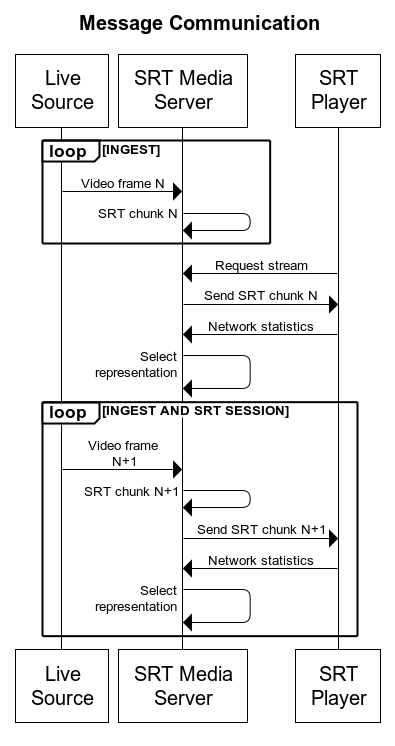
\includegraphics[width=0.6\textwidth,keepaspectratio]{webseq.png}
	\caption{Sequence diagram.}
	\label{fig:BMSB2020sequence}
\end{figure}

The communication between the systems in the setup is shown in Figure \ref{fig:BMSB2020sequence}. SRT Media Server starts to encode and packetize video frames when the Live Source is connected. Video frames are H.264 encoded and MPEG-TS muxed, then packetized into SRT chunks.
Nevertheless, data are not transmitted until an SRT player connects to the SRT Media Server. It means that chunks can be discarded by the server if there are no players. The SRT Media Server only stores the most recent chunks with a buffer size of "maximum allowed latency". This operation is necessary in order to guarantee that only the most recent chunks are sent, then achieve a low latency live streaming. In GStreamer, maximum allowed latency is configurable, but we decide to keep it to its default value which is 125 ms. Once the SRT player is connected, SRT Media Server starts delivering the content to the player. While receiving the content, the SRT player stores it in the playback buffer before decoding and displaying it. The playback buffer is set to 1 seconds to balance low latency, packet losses reliability and changeable network conditions.

To adapt the representation, the implemented Adaptive Rate Control accesses network statistics from the SRT server sink plugin and exploits the information to tune the configuration of the H.264 encoder. This evaluation is performed by the Adaptive Rate Control once per second. The decision algorithm of the implemented Adaptive Rate Control is shown in Algorithm \ref{alg:BMSB2020algorithm}. The algorithm takes the last measured network bandwidth (\textit{bw$_t$}), round-trip delay time (\textit{rtt$_t$}) and send rate (\textit{rate$_t$}) from SRT network reports, the current employed representation level (\textit{rep$_t$}) and the list of all the available ones (\textit{\{rep$_{list}$\}}). Bandwidth and round-trip delay time are employed to evaluate the maximum allowed network throughput (\textit{throughput$_{max_t}$}) through the Equation \ref{eq:BMSB2020thoughput}.

\begin{algorithm}
	\renewcommand{\algorithmicrequire}{\textbf{Input:}}
	\renewcommand{\algorithmicensure}{\textbf{Output:}}
	\caption{Adaptive Rate Control}
	\label{alg:BMSB2020algorithm}
	\begin{algorithmic}
		\Function{adaptiveRate}{bw$_{t}$, rtt$_{t}$, rate$_{t}$, rep$_{t}$, $\{rep_{list}\}$}
		\Require bw$_t$ \Comment{measured bandwidth}
		\Require rtt$_t$ \Comment{measured delay}
		\Require rate$_t$ \Comment{measured send rate}
		\Require rep$_t$ \Comment{current representation}
		\Require $\{rep_{list}\}$ \Comment{available representations}
		\Ensure rep$_{t+1}$ \Comment{next representation}
		\State throughput$_{max_t}$ $\leftarrow$ bw$_{t}$, rtt$_{t}$ \Comment{network throughput}
		\ForAll { rep$^{i}$ $\in$ $\{rep_{list}\}$ } \Comment{for each representation}
		\State bitrate$^{i}_{t}$ $\leftarrow$ rep$^{i}$, rate$_{t}$, rep$_t$ \Comment{\parbox[t]{0.31\linewidth}{minimum network bitrate}}
		\If {(throughput$_{max_t}$ $>$ throughput$^{i}_{t}$)} %\Comment{\parbox[t]{0.1\linewidth}{network admits the bitrate}}
		\State \Comment{network admits the representation}
		\State rep$_{t+1}$ $\leftarrow$ rep$^i$ \Comment{next representation}
		\EndIf
		\EndFor
		\EndFunction
	\end{algorithmic}
\end{algorithm}

\begin{equation}
\label{eq:BMSB2020thoughput}
throughput_{max_t} = bw_t * \frac{1}{1 + \frac{rtt_t}{2}}
\end{equation}

Then, for each available representation, the required network throughput to allow its transmission is calculated. It is important to note that each representation means a different throughput configured by the encoding bitrate. Furthermore, the encoding bitrate needs to accommodate a gap to allow that protocols messages and extra information from other levels of the ISO/OSI model, added to the encoded video payloads, still meet network bandwidth thresholds.

Consequently, to establish if it is possible to stream a specific representation to the client, we should compare the maximum allowed network throughput (\textit{throughput$_{max_t}$}) with the throughput that the representation would generate (\textit{throughput$^i_t$}). Since we cannot access the employed throughput before streaming the content, we estimate it from the current send rate (\textit{rate$_t$}) provided by the network reports. Equation \ref{eq:BMSB2020minBW} estimates the necessary network throughput (\textit{throughput$_t^i$}) to allow the representation (\textit{rep$^i$}) bitrate to be streamed. The ratio between current send rate (\textit{rate$_t$}) and current representation encoding bitrate (\textit{rep$_t$}) is the current overhead, then we multiply it per the representation encoding bitrate (\textit{rep$^i$}).

\begin{equation}
\label{eq:BMSB2020minBW}
%bitrate^{i}_{t} = rep^i * \frac{rate_{t}}{rep_{t}}
throughput^{i}_{t} = rep^i * \frac{rate_{t}}{rep_{t}}
\end{equation}

If the estimated throughput (\textit{throughput$_t^i$}) is lower than the maximum allowed throughput (\textit{throughput$_{max_t}$}), it means that the representation can be sent. The output of the algorithm is the selected representation to be employed at the H.264 encoder. The encoder is configured to immediately generate a \textit{keyframe} and switch at the new selected representation resolution and encoding bitrate.

\subsection{Results}
\label{sec:BMSB2020results}

The experimental setup employed for testing the implemented Adaptive Rate Control is presented in Figure \ref{fig:BMSB2020setup}. The overall setup comprises the following nodes:
\begin{itemize}
	\item STR Media Server and Traffic Control: this is a unique physical node which embeds two logical systems. We employ a Docker containerization \cite{merkel2014} to run different functions in separated environments. A Docker container running Ubuntu 19.04 OS includes the Adaptive Rate Control-enabled SRT Media Server developed through GStreamer framework \cite{gstreamer}. The container communicates with the host machine running Ubuntu 16.04 OS which forwards data to the physical network interface. On the host machine, we periodically modify bandwidth and latency of the network interface. Traffic Control \cite{tc} is the utility to change the uplink capacity. To emulate an LTE network, we use the \textit{European Broadband user experience} dataset collected and publicly provided by the Joint Research Centre (JCR) of the European Commission \cite{chawdhry2016}. The dataset provides both bandwidth and latency that we apply through Traffic Control utility. The interval between two consecutive network changes is set to 100 ms. %, aligned with the dataset sample rate.
	\item Network switch: this node provides wired network access to both server and player nodes to communicate each other. It forwards all the incoming traffic on both sides.
	\item SRT Player: this node run a GStreamer application to receive the SRT stream and play it.
\end{itemize}

\begin{figure}[htp]
	\centering
	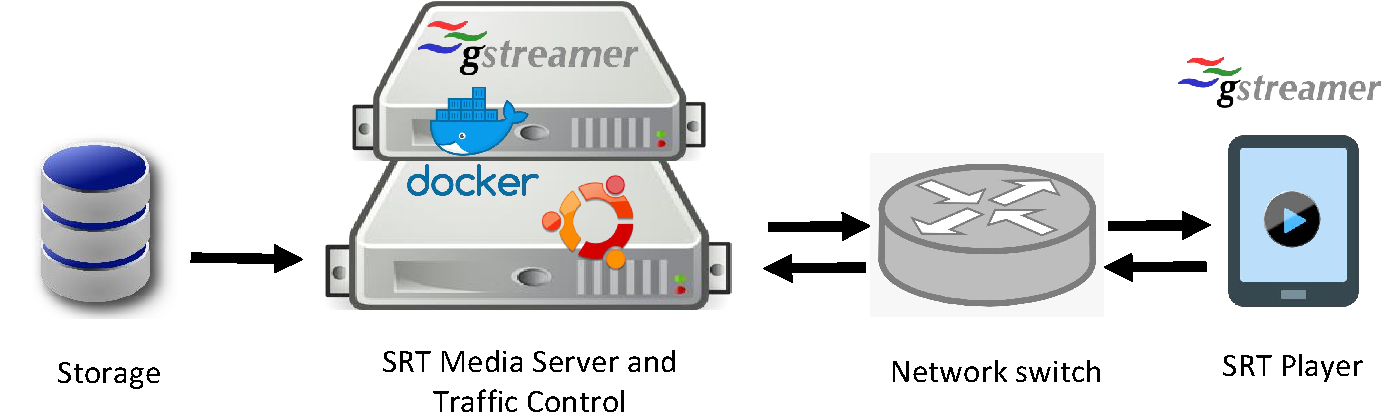
\includegraphics[width=1\textwidth,keepaspectratio]{testbed.pdf}
	\caption{Experimental setup.}
	\label{fig:BMSB2020setup}
\end{figure}

\begin{table}[htp]
	\caption{Set of representations employed in the experiments.}
	\centering
	\bgroup
	\def\arraystretch{1.2}%  1 is the default, change whatever you need
	\setlength\tabcolsep{2.5pt} % default value: 6pt
	\label{tab:BMSB2020reps}
	{\scriptsize
		\begin{tabular}{>{\centering\arraybackslash}m{\dimexpr0.1\textwidth-2\tabcolsep-\arrayrulewidth\relax}
				>{\centering\arraybackslash}m{\dimexpr0.15\textwidth-2\tabcolsep-\arrayrulewidth\relax}
				>{\centering\arraybackslash}m{\dimexpr0.15\textwidth-2\tabcolsep-\arrayrulewidth\relax}
				>{\centering\arraybackslash}m{\dimexpr0.15\textwidth-2\tabcolsep-\arrayrulewidth\relax}
			}
			\toprule
			\textbf{Index} & \textbf{bitrate (kbps)} & \textbf{resolution} & \textbf{framerate (FPS)} \\
			\midrule
			\midrule
			1 & 1200 & 640x360 & 24 \\
			2 & 2250 & 1280x720 & 24 \\
			3 & 4500 & 1920x1080 & 24 \\
			\bottomrule
			\bottomrule
		\end{tabular}
		\egroup
	}
\end{table}

We perform different experiments to compare the Adaptive Rate Control-enable SRT stream with a legacy SRT stream. We use a locally stored Big Buck Bunny test sequence to feed the SRT Media Server. Its raw version is provided by Xiph.Org Foundation \cite{xiph}. For the Adaptive Rate Control-enabled stream, we established three different representation levels to be employed by the H.264 encoder, while legacy one employs only the higher one. The representations are shown in Table \ref{tab:BMSB2020reps}.

The duration of each SRT streaming session lasts 594 seconds which is the duration of the employed test sequence. The results of the two strategies in terms of representation switches, freezes, initial delay and average representation bitrate are shown in Table \ref{tab:BMSB2020results}.

\begin{table}[htp]
	\caption{Number of switches (\textit{S$_{Nb}$}), number of freezes (\textit{F$_{Nb}$}), average freeze duration (\textit{F$_{avg}$}), initial delay (\textit{D}) and average representation bitrate (\textit{R$_{avg}$}) for both legacy and Adaptive Rate Control-enabled SRT streams.}
	\centering
	\def\arraystretch{1.2}%  1 is the default, change whatever you need
	\setlength\tabcolsep{2.5pt} % default value: 6pt
	\label{tab:BMSB2020results}
	{\scriptsize
		\begin{tabular}{>{\centering\arraybackslash}m{\dimexpr0.2\textwidth-2\tabcolsep-\arrayrulewidth\relax}
			>{\centering\arraybackslash}m{\dimexpr0.1\textwidth-2\tabcolsep-\arrayrulewidth\relax}
			>{\centering\arraybackslash}m{\dimexpr0.1\textwidth-2\tabcolsep-\arrayrulewidth\relax}
			>{\centering\arraybackslash}m{\dimexpr0.1\textwidth-2\tabcolsep-\arrayrulewidth\relax}
			>{\centering\arraybackslash}m{\dimexpr0.1\textwidth-2\tabcolsep-\arrayrulewidth\relax}
			>{\centering\arraybackslash}m{\dimexpr0.1\textwidth-2\tabcolsep-\arrayrulewidth\relax}
		}
		\toprule
		\textbf{SRT server} & \textbf{S$_{\textbf{Nb}}$} & \textbf{F$_{\textbf{Nb}}$} & \textbf{F$_{\textbf{avg}}$(ms)} & \textbf{D(ms)} & \textbf{R$_{\textbf{avg}}$(kbps)}\\
		\midrule
		\midrule
		Legacy & 0 & 122 & 820 & 972 & 4500 \\
		Adaptive Rate Control & 197 & 87 & 727 & 986 & 4028 \\
		\bottomrule
		\bottomrule
	\end{tabular}
	}
\end{table}

\begin{figure}[htp]
	\centering 
	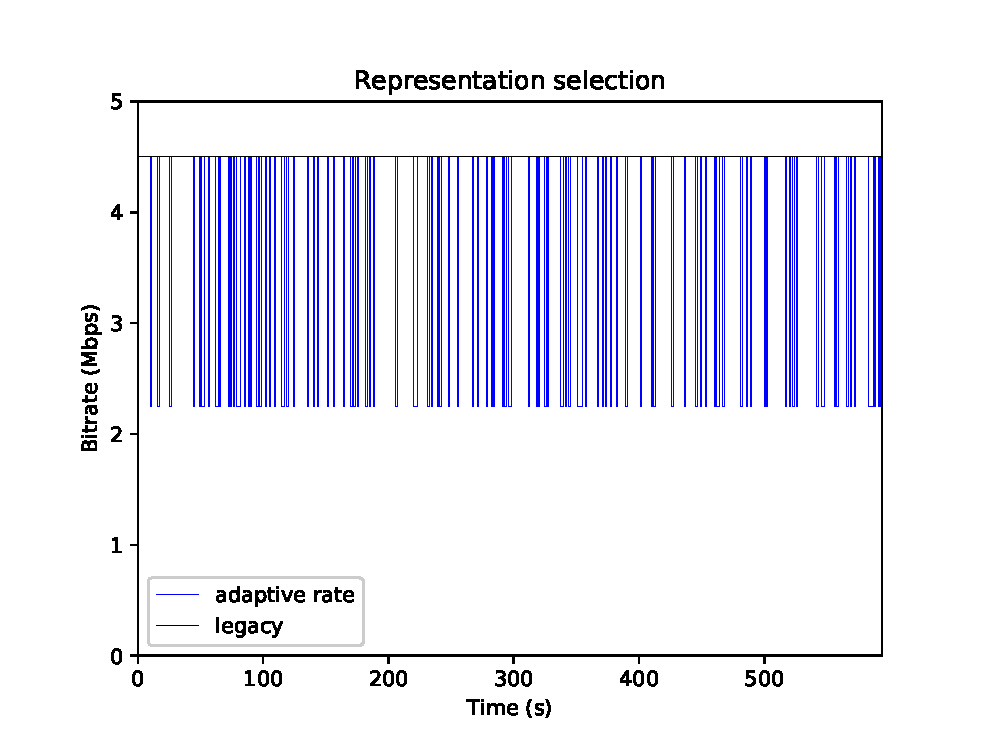
\includegraphics[width=1\textwidth,keepaspectratio]{reps.eps}
	\caption{Representation bitrate selection.}
	\label{fig:BMSB2020selection}
\end{figure}

In terms of switches, Adaptive Rate Control solution performs 197 representation switches, while it is not applicable to the legacy SRT stream. Figure \ref{fig:BMSB2020selection} shows the distribution of the switches across the streaming session. Legacy stream is stable to 4500 kbps encoding bitrate, while seems that Adaptive Rate Control one never uses the lowest encoding bitrate (1200 kbps) but moves between the other two (4500 and 2250 kbps). Thus, it causes that the average representation bitrate is 10\% lower when using the Adaptive Rate Control (4028 kbps against 4500 kbps). In terms of initial delay, there is not a noticeable difference since the Adaptive Rate Control does not introduce any delay while starting the streaming session. On the contrary, our Adaptive Rate Control solution outperforms legacy one while considering number of freezes and their duration. Here, the proposed solution scores 29\% less freezes events, and their average duration is 11\% shorter.

These results show that our solution sacrifices average representation bitrate in order to reduce freezes events. Fewer freezes events lead to a smoother video playback for the end user.

\subsection{Conclusions and Future Work}
\label{sec:BMSB2020conlusion}
This paper proposes an Adaptive Rate Control for SRT protocol to deliver live streaming content, while coping with transmission variability due to network degradation or issues.

The proposed solution is integrated with Open Source GStreamer multimedia framework and tested by altering the network capabilities according to real LTE measurements provided by a publicly available dataset.

Compared to a legacy SRT solution, the results show that Adaptive Rate Control-enabled SRT delivery experiences fewer freeze events by enabling switching operations to lower representation bitrates. Thus, it reduces the average representation bitrate to prioritize playback smoothness.


% use section* for acknowledgement
%\subsection*{Acknowledgment}
% !TeX spellcheck = en_US
%Publications.tex
\newcommand{\PublicationsPath}{PatentsAndPublications/Publications}

%BMSB2019

\section[QoE-based enhancements of Chunked CMAF over low latency video streams]{QoE-based enhancements of Chunked CMAF over low latency video streams}
\label{chap:BMSB2019}
\begin{itemize} \itemsep1pt\parskip0pt\parsep0pt
	\item \textbf{Title:} QoE-based enhancements of Chunked CMAF over low latency video streams
	\item \textbf{Authors:} Roberto Viola, Alvaro Gabilondo, \'Angel Mart\'in, Juan Felipe Mogoll\'on and Mikel Zorrilla
	\item \textbf{Proceedings:} 2019 IEEE International Symposium on Broadband Multimedia Systems and Broadcasting (BMSB)
 	\item \textbf{Publisher:} IEEE
	\item \textbf{Year:} 2019
	\item \textbf{DOI:}  \url{10.1109/BMSB47279.2019.8971894}
\end{itemize}	

\textbf{Abstract:} 5G infrastructures are in the roadmap of content delivery services, aiming to forward all broadcast and broadband video traffic using a common telecommunication network architecture. Streaming services will benefit from 5G networks which promise higher capacity, higher bandwidth and lower latency than current infrastructures. However, the widely employed streaming technologies, such as Dynamic Adaptive Streaming over HTTP (MPEG-DASH), require an intrinsic high latency of tens of seconds to enforce the Quality of Experience (QoE). These conditions turn MPEG-DASH unfavourable when compared with a traditional broadcast pipeline for live events in terms of latency. Therefore, improvements on latency of streaming technologies are necessary to deliver live broadcast services over 5G networks. The media industry proposed a Chunked Common Media Application Format (Chunked CMAF) in order to achieve latency under a second. In this paper, we show an implementation of a Chunked CMAF for MPEG-DASH live videos in a real deployment. To further evaluate the benefits of CMAF we evaluate the QoE results when delivering a legacy MPEG-DASH live content compared to a Chunked CMAF-powered one.

\textbf{Keywords:} Chunked CMAF, Future broadcasting services, MPEG-DASH, Quality of Experience, Video coding and processing.

\subsection{Introduction}
% no \IEEEPARstart
Video streaming services represent a large fraction of the Internet traffic. In fact, live video traffic will grow 3-fold from 2017 to 2022, accounting the 17\% of all internet video traffic \cite{ciscovideo2017}. This trend would be fuelled by the deployment of 5G networks, which will enable the cooperation between broadband and broadcast services \cite{calabuig2015}.

5G networks promise high capacity, high bandwidth and low latency to cope with demanding traffic and services. Nevertheless, MPEG-DASH and other HTTP-based alternatives require to packetize video contents in segments with a duration in the order of seconds to enforce the QoE, leading to tens of seconds of delay between content generation and consumption \cite{lohmar2011}. This delay is produced by the duration of packaged media segments, designed to match changeable network delivery performance, and the required buffering, done by the media player to achieve a smooth playback for \mbox{on-demand} and live streams. This delay is not significant for \mbox{on-demand} contents, but it is too high to deliver live streams with comparable performance to the broadcast live services. Moreover, when deploying hybrid broadcast broadband services, the common mechanism to synchronize broadcast and broadband signals consists in delaying the broadcast source as broadband stream is usually 30-40 seconds delayed with respect to the broadcast service.

The Common Media Application Format (CMAF) \cite{hughes2017information}, proposed by ISO/IEC, is the solution for delivering live contents from media industry. CMAF includes two major benefits. First, it ensures the use of the ISO Base Media File Format, usually referred as MP4, as a common file format when combined with different streaming technologies such as MPEG-DASH or HTTP Live Streaming (HLS). This feature makes media storage more efficient as different manifests (MPD for MPEG-DASH and M3U8 for HLS) may index the same segments. Each media client can download a different manifest depending on its supported streaming technologies. Then, it plays the content by downloading the same media segments. Thus, the server needs lower storage capacity. Secondly, it defines a chunked mode, named Chunked CMAF or Low Latency CMAF, which enables latency enhancement of the stream, reducing the time elapsed between media packaging and its playback.

\begin{figure}[htp]
	\centering
	
\includegraphics[width=1\textwidth,keepaspectratio]{CMAF.eps}
	\caption{Legacy fragment and Chunked CMAF fragment.}
	\label{fig:BMSB2019fragment}
\end{figure}

Typical MPEG-DASH media segments contain a single MP4 fragment with the fragment duration equal to the segment duration. Here, common values for segment duration are from 2 to 30 seconds. On the contrary, Chunked CMAF enables a single segment to contain multiple fragments as depicted in Figure \ref{fig:BMSB2019fragment}. Therefore, Chunked CMAF exploits the use of short MP4 fragments, including the minimum data required by the player to start decoding the stream. Therefore, the shorter fragment duration allows a promptly playback start, removing the limitation to fully download the entire segment. 

This work proposes a real implementation of a server-client solution delivering Chunked CMAF streams of live contents. This solution has been achieved by providing two relevant contributions:
\begin{itemize}
	\item Chunked CMAF has been integrated with an Open Source MPEG-DASH framework.
	\item The evaluation measures the effects on user's QoE while varying the fragment duration of the Chucked CMAF segments and the resulting latency.
\end{itemize}

The remainder of this paper is organized as follows. First, section \ref{sec:BMSB2019related} presents the background of the MPEG-DASH standard and Chunked CMAF for deploying live media services. Then, section \ref{sec:BMSB2019implementation} shows the implementation of Chunked CMAF solution. In section \ref{sec:BMSB2019results} we describe the experiments and present the results. Finally, in section \ref{sec:BMSB2019conlusion} we expose the conclusions and future work.

\subsection{Related Work}
\label{sec:BMSB2019related}
In this section, it is included an overview of MPEG-DASH for live streaming services and afterwards, a comprehensive review about the State of Art of Chunked CMAF is described.

\subsubsection{Overview of Live MPEG-DASH}
\label{sec:BMSB2019dash}
MPEG-DASH was developed by MPEG and standardized by ISO/IEC. In MPEG-DASH, first, the client fetches a Media Presentation Description (MPD) and parses it to be aware of the different representations of the content. Then, the player chooses the representation that fits in the device capabilities in terms of resolution, language, codec and bitrate. Accordingly, the client requests and downloads the corresponding segment from the server. Once a segment has been played, the next one from the MPD is requested. During the playback, the player can switch to a different representation depending on its preferences and network performance in order to minimize any impact on the QoE.

The live playback is possible through the \textit{availabilityStartTime} field in the MPD, which marks the UTC time when the stream is made available. The client continuously compares it with the current time to fetch the last available segments. In the case of a legacy live MPEG-DASH content, the \textit{availabilityStartTime} has to correspond to the time when the first media segment is fully available on server side. Then, the segment duration, which ranges from 2 to 30 seconds, is the minimum delay that a client experiences during a live stream. Encoding and network latency also influence this delay, but their weights in the resulting latency are 10-100ms when aggregated to the segment duration.

\subsubsection{Chunked CMAF}
\label{sec:BMSB2019cmaf}
The latency is a key factor when dealing with live streaming contents. Current MPEG-DASH-based solutions are not able to operate with a similar latency to the current broadcast solutions. This is a major challenge when targeting broadcast levels of QoE. The use of Chunked CMAF, together with improved network bandwidth and latency of the 5G networks, aims to reduce live streaming latency and keep it behind a second \cite{bouzakaria2014overhead}.

Contrary to the legacy MPEG-DASH streams, a Chunked CMAF-compliant MPEG-DASH distinguishes between MP4 fragment duration and media segment duration with different values. The reduction of the fragment duration makes the media units of the stream quickly available enabling prompt playback. Consequently, the segment contains multiple fragments and the \textit{availabilityStartTime} attribute contained in the MPD must be set at the time the first fragment is available, even if the segment is not completely written. The smaller the fragment is, the smaller delay is experienced by the player. Theoretically, fragment duration can be reduced to one frame duration. To this end, it is required a proper server, which must be able to split the HTTP response sending fragment units instead of the full segment.

Several implementations serve Chunked CMAF with \mbox{HTTP 1.1} Chunked Transfer Encoding. The server encapsulates each MP4 fragment in a HTTP chunk and deliver it over time, instead of sending the entire segment at once. In \cite{saminathan2011}, Chunked Transfer Encoding allows a \mbox{HTTP 1.1} server to split the response in small HTTP chunks. The paper shows that the latency does not depend on the segment duration but depends on the duration chosen for the HTTP chunks. This approach still uses one second duration chunks while splitting the HTTP connection between server and player. The author of \cite{essaili2018} also implements a MPEG-DASH delivery involving Chunked CMAF, but it varies the duration of the fragment. Both papers provide performance results in terms of overall latency.

The work shown in \cite{wei2014} uses HTTP 2.0 to exploit the \mbox{push-mode} added in the new HTTP version for reducing the latency. HTTP 2.0 does not have a Chunked Transfer \mbox{Encoding} mode, since it already employs a frame-based \mbox{delivery}, i.e. it splits the response in several frames which contain the Chunked CMAF MP4 fragments. This solution has the \mbox{advantage} of reducing the protocol header overhead since HTTP 2.0 header is simplified when compared to HTTP 1.1. However, push-mode reduces the adaptation possibilities at the client-side to dynamically select an appropriate representation for the network performance conditions. Decisions can be still done by the server, modifying the MPD, but this approach does not scale as the player-side decisions when working in pull-mode.

\subsubsection{QoE Metrics}

The reduction of the latency of the service is the major goal to all these scientific approaches. Nevertheless, when evaluating streaming services, it is essential to focus in user's QoE. The QoE is a key aspect for user satisfaction and retention when rating streaming services. Hence, any solution trying to enhance media delivery needs to consider QoE metrics. No one of the above works consider QoE as a metric in order to evaluate the real benefits to end users.

A commonly used scale to evaluate QoE is the Mean Opinion Score (MOS) which consists of five increasing quality levels (from 1 to 5) \cite{Itu2016}. In the literature many models are available to profile the subjective human perception of the quality and estimate the MOS through objective metrics. In \cite{claeys2014} the author uses metrics like initial delay, stalling time, number of representation switches and inter-switching times in order to get an estimated Mean Opinion Score (eMOS). This eMOS quantifies the quality of video streaming services based on objective streaming connectivity and buffering measures of players without a demographic perception study of users. In \cite{hossfeld2012} the author proposes to evaluate the MOS depending on the initial delay and the numbers of freezes. It concludes that is preferable a higher initial delay than freezes in order to have a better human perception. Recently, the work \cite{lentisco2017} investigates a new model for MOS, called Ubiquitous-Mean Opinion Score for Video (U-vMOS), which makes initial buffering more dominant than \cite{claeys2014}.

\subsection{Chunked CMAF Implementation}
\label{sec:BMSB2019implementation}

\subsubsection{System Model}
\label{sec:BMSB2019system}

The implemented end-to-end system for delivering Chunked CMAF MPEG-DASH streams is depicted in Figure \ref{fig:BMSB2019system}. The system is composed by the following nodes: Video ingest, Media Packager, HTTP Server and DASH Player.

\begin{figure}[htp]
	\centering
	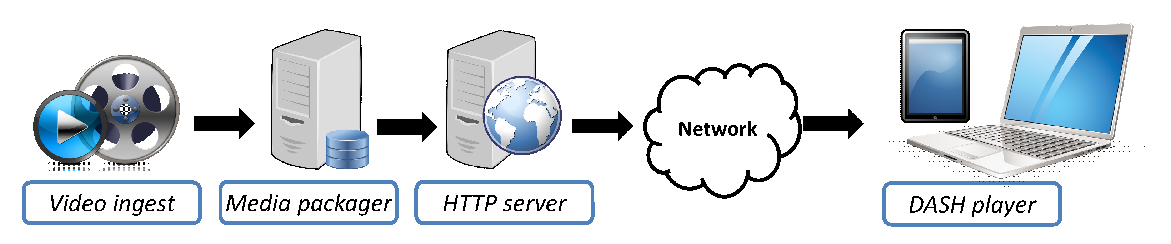
\includegraphics[width=1\textwidth,keepaspectratio]{system.eps}
	\caption{End-to-End DASH streaming system.}
	\label{fig:BMSB2019system}
\end{figure}

Video ingest is the system which injects the content into the processing and delivery chain. Many and different entities can act as a live source for media production, e.g. a live camera or any video software editor.

Media Packager is based on GStreamer \cite{gstreamer}. It is in charge of processing the content ingested and generating a standard compliant Chunked CMAF MPEG DASH stream. It encodes the content, packetizes it into MP4 fragments and segments and creates a live DASH Media Presentation Description (MPD) to expose the stream to the clients. The recent stable GStreamer release (v1.14) does not provides capabilities for generating a Chunked CMAF steam. Then, to experiment with Chunked CMAF, we introduced additional features and properly tuned the following plugins based on GStreamer v1.5:

\begin{itemize}
	\item \textit{H264 encoder}: the performance and setup of the encoder is key to favour a low latency stream, enabling the player to request the last generated MP4 fragment and to start its playback. \textit{Keyframes} (I-frames) do not require any other frames to be decoded, so the player has to start decoding a stream from a \textit{keyframe}. Thus, \textit{keyframes} are essential for live streaming and each generated fragment should start with a \textit{keyframe} to boost the playback start. The Group of Pictures (GOP) is a collection of successive pictures within a coded video stream where the \textit{keyframe} always indicates the beginning of a GOP. In terms of header information, some fields are mandatory for playing the stream, e.g. Sequence Parameter Set (SPS) and Picture Parameter Set (PPS) provide basic parameters like the frame size. Consequently, we encode the content forcing the presence of a \textit{keyframe} and all the header information at the beginning of each MP4 fragment. Moreover, for the remaining frames we avoid to use bidirectional predicted frames (B-frames) since they add additional latency into the encoding process due to required frames reorder. The resulting stream contains only key and predicted frames (I-frames and P-frames).
	\item \textit{MP4 muxer}: it packetizes the encoded frames into MP4 fragments and segments. Since we established that each fragment contain only one GOP, with a \textit{keyframe} at the beginning, the muxer works by switching from a fragment to another each time it recognizes a \textit{keyframe} generated by the encoder. In case a minimum theoretical latency wants to be exercised, putting bandwidth efficiency aside for unlimited connectivity, the encoder could just use \textit{keyframes}, i.e. no predicted frames are used, meaning the MP4 fragment contains just one frame. According to the specifications, each fragment contains header information (moof) and a payload (mdat) with the encoded data.
	\item \textit{MPEG-DASH filesink}: it receives the MP4 fragments from the muxer and aggregates them in order to write the segments on the disk. Since the fragments can be decoded independently each other, the fragments are concatenated by appending the new fragment at the end of the previous one. Following this strategy, it is not necessary to receive all the fragments to start writing a segment, which is progressively written on the disk. The filesink also creates the MPD manifest which contains the URL where the player can download the last fragment or, in case of legacy live MPEG-DASH stream, the segment. The filesink also updates the \textit{availabilityStartTime} field of the MPD manifest to allow the player to calculate the last generated fragment (or segment) time with accuracy and to download it. The generated MPD and the segments are directly written by the filesink in the storage of the HTTP Server.
\end{itemize}


HTTP Server is based on Node.js \cite{nodejs}. It is in charge of serving the content generated by the Media Packager to the player. When the player connects to the HTTP Server, the server loads the content from its storage and serves each fragment promptly to the player. Its functions include:
\begin{enumerate}
	\item It loads partial segments which are still being generated by Media Packager.
	\item It analyzes a segment and recognizes the contained MP4 fragments.
	\item It serves the fragments to the client through HTTP 1.1 chunked transfer encoding. Each HTTP chunk contains one fragment.
	%\item In case the player requests are not perfectly synchronized and the required fragment is not available, it waits until the fragment is generated in order to serve it.
\end{enumerate}

DASH player is based on the last stable GStreamer release (v1.14) \cite{gstreamer}. This version already provides capabilities to parse the manifest and request the last generated segment, then decoding and displaying it. Thus, it is able to play legacy MPEG-DASH streams. Moreover, GStreamer HTTP source plugin is able to receive a HTTP 1.1 chunked response when using a fragmented segment, but it does not pass the downloaded fragments to the decoding pipeline until it receives the whole segment. Thus, this is not valid in case of low latency streaming and the implementation of a Chunked CMAF Media Packager and HTTP Server would not be applicable. On the contrary, the HTTP source can request a section of a file if the exact byte range of the fragment inside a segment is known. The player can request the fragments separately and forward it to the decoding pipeline. Consequently, we modify the capabilities of the Media Packager in order to add \textit{mediaRange} \cite{mediarange} attributes inside the manifest which explicitly provides the DASH Player the byte range of the fragment. The player parses this attribute and requests separately the fragments to the server by adding Range header \cite{range} into the HTTP 1.1 request. The HTTP Server receives the requests, analyzes the segment and send the fragment included in the chosen range. When the player receives the fragment, it forwards the fragment to the decoding pipeline. Furthermore, to reduce latency, it is also important to take into account the internal playout buffer at the player since it is a widely used mechanism for preventing image freezes. However, it adds delay when playing the content. To overcome this limitation, we tuned the buffer size to be equal to one fragment duration. Finally, to synchronize the player and calculate the last fragment time with accuracy, we employ the network time protocol (NTP) to keep the Media Packager at server side and player device at client side synchronized. To sum up, the player does the following tasks:
\begin{enumerate}
	\item It parses the MPD manifest in order to get the \textit{availabilityStartTime}
	\item It compares the \textit{availabiltyStartTime} with NTP clock time in order to know which is the last generated fragment or, in case of legacy MPEG-DASH stream, segment.
	\item It requests the last generated fragment (or segment) from the HTTP Server.
	\item It decodes and displays the received stream.
\end{enumerate}

The communication between the nodes of the system is shown in Figure \ref{fig:BMSB2019sequence}.

\begin{figure}[htp]
	\centering
	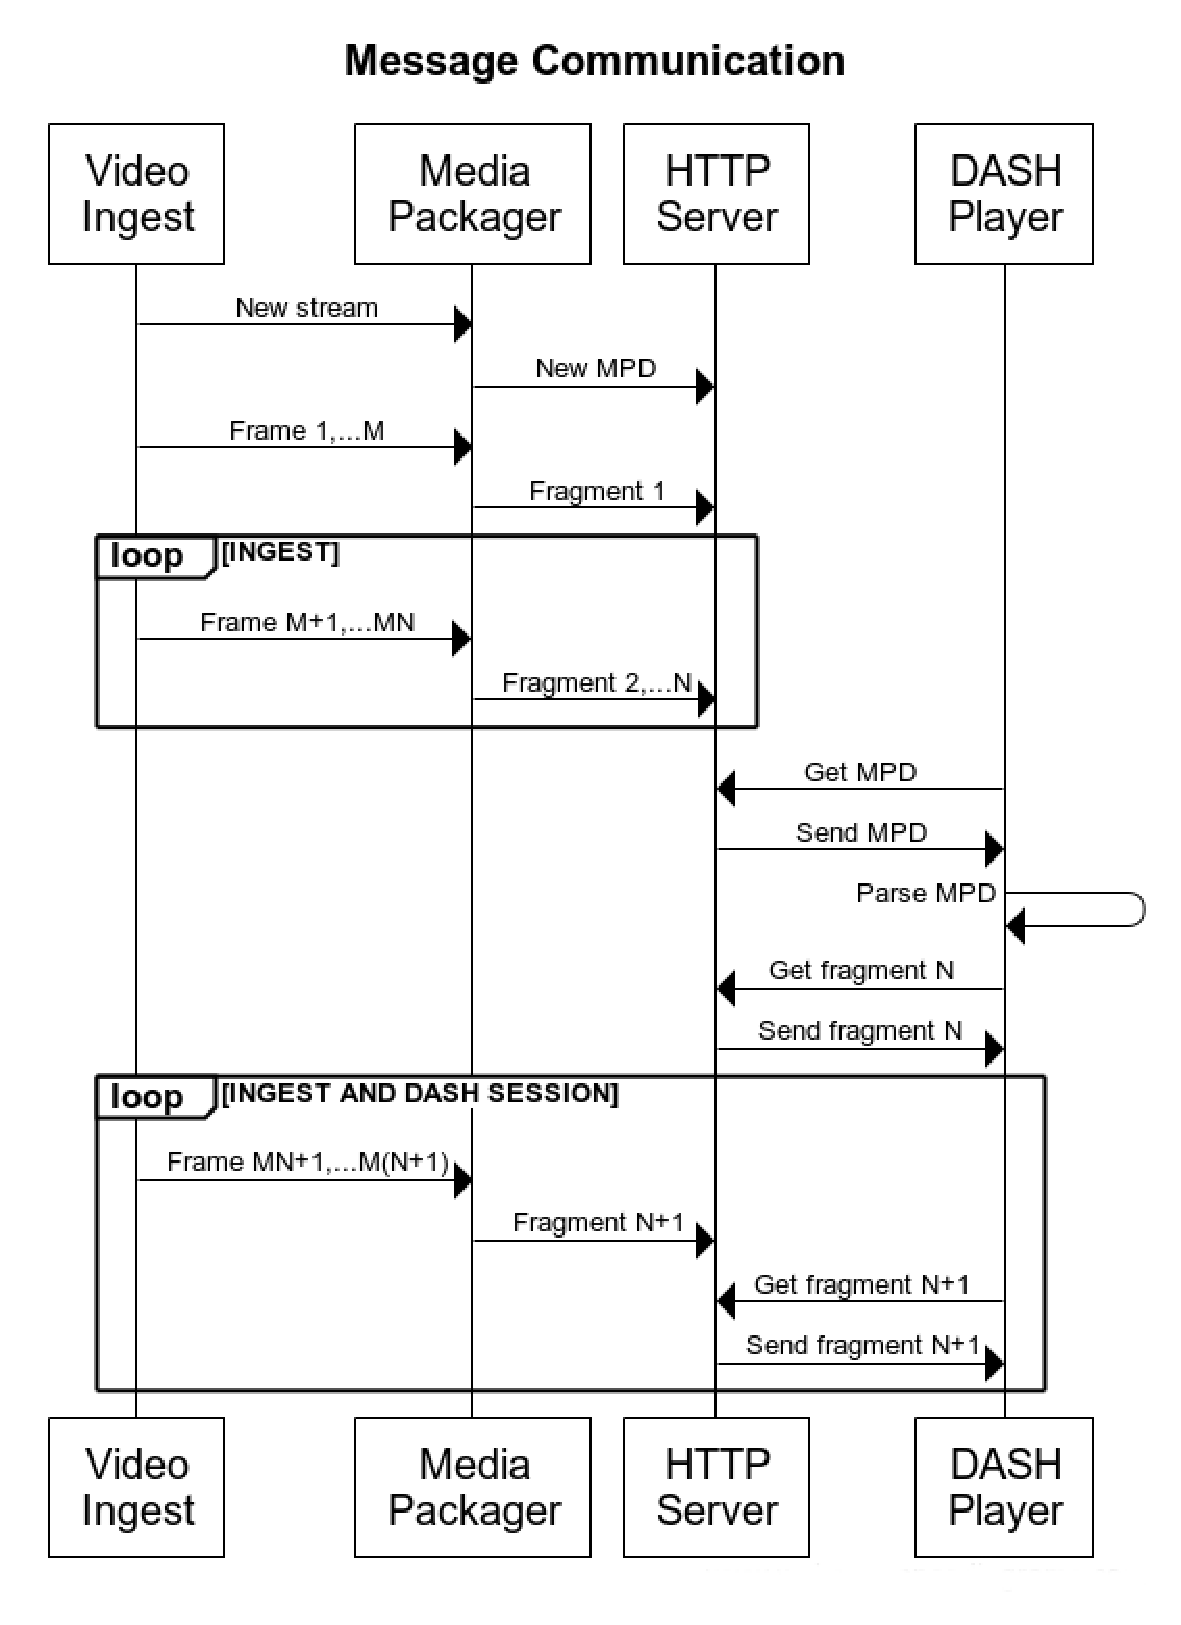
\includegraphics[width=0.7\textwidth,keepaspectratio]{webseq3.eps}
	\caption{Sequence diagram.}
	\label{fig:BMSB2019sequence}
\end{figure}

Media Packager begins to encode and packetize the content into MP4 fragments when the live source is connected.
The Chunked CMAF content is directly stored inside the storage located at the HTTP Server. Meanwhile the content is generated, the clients can connect to the HTTP Server which serves the segments.

\subsubsection{QoE Metrics}
\label{sec:BMSB2019measurement}

The measurements of the implemented solution aim to identify the effects on QoE. From the work of Claeys et al. \cite{claeys2014}, the QoE is related to objective metrics such as frequency and duration of freezes that we can measure directly introducing some probes into the player while playing the content. We consider that the playback freezes when the internal buffer of the player goes empty and defines the duration of the freeze the time between the buffer goes empty and it starts to refill.

Moreover, Hossfeld et al. \cite{hossfeld2012} investigates the effects of playout delay on the user and concludes that the user's satisfaction decreases while the playout delay increases. The playout is the elapsed time between the moment the user pushes the play button and the first frame is displayed on the screen. Anyway, in case of low latency, the playout depends also on content generation since the player needs to synchronize with sender. Consequently, in case of low latency steaming, it is more useful to measure the end-to-end latency of the system. From the work of Essaili et al. \cite{essaili2018}, the latency is the elapsed time between the frame ingest at the Media Packager (T$_{in}$) and the visualization time on the player screen (T$_{out}$), it can be express through the Expression \ref{eq:BMSB2019latency}.

\begin{equation}
\label{eq:BMSB2019latency}
Latency = T_{in} - T_{out} = T_{enc} + d_F + T_{fetch} + T_{dec}
\end{equation}

The latency depends on processing time at Media Packager (T$_{enc}$), the fragment duration (d$_F$), the time for fetching the fragment from HTTP Server (T$_{fetch}$) and the decoding time at the player (T$_{dec}$).

We evaluate the latency of the end-to-end system by summing up all the components which appear in the Equation (\ref{eq:BMSB2019latency}). Since in case of live streaming the Media Packager should work on real-time, T$_{enc}$ is inversely proportional to the input framerate. Accordingly, T$_{enc}$ is considered a fixed value. In the next section the remaining values of Equation (\ref{eq:BMSB2019latency}) are evaluated.

\subsection{Results}
\label{sec:BMSB2019results}

To test the implemented end-to-end Chunked CMAF solution, a live MPEG-DASH dataset using Big Buck Bunny test sequence was employed. Its raw version is provided by Xiph.Org Foundation \cite{xiph}. The raw video was encoded in H264/AVC format (ISO/IEC23008-2:2015). Then, it is multiplexed in ISO MPEG4 fragments (ISO / IEC 14496-12 - MPEG-4 Part 12) and split into segments. We experiment with the different representation levels shown in Table \ref{tab:BMSB2019reps}.

\begin{table}[htp]
	\caption{Set of MPEG-DASH representations employed in the experiments.}
	\centering
	\bgroup
	\def\arraystretch{1.2}%  1 is the default, change whatever you need
	\setlength\tabcolsep{2.5pt} % default value: 6pt
	\label{tab:BMSB2019reps}
	\def\arraystretch{1.2}%  1 is the default, change whatever you need
	\setlength\tabcolsep{2.0pt} % default value: 6pt
	{\scriptsize
		\begin{tabular}{>{\centering\arraybackslash}m{\dimexpr0.1\textwidth-2\tabcolsep-\arrayrulewidth\relax}
			>{\centering\arraybackslash}m{\dimexpr0.15\textwidth-2\tabcolsep-\arrayrulewidth\relax}
			>{\centering\arraybackslash}m{\dimexpr0.15\textwidth-2\tabcolsep-\arrayrulewidth\relax}
			>{\centering\arraybackslash}m{\dimexpr0.15\textwidth-2\tabcolsep-\arrayrulewidth\relax}
		}
		\toprule
		\textbf{Index} & \textbf{bitrate} & \textbf{resolution} & \textbf{framerate} \\
		\midrule
		\midrule
		1 & 1200kbps & 352x288 & 30fps  \\
		2 & 1600kbps & 640x360 & 30fps  \\
		3 & 2250kbps & 960x540 & 30fps \\
		4 & 2000kbps & 704x576 & 30fps \\
		5 & 4500kbps & 1280x720 & 30fps \\
		6 & 8000kbps & 1920x1080 & 30fps \\
		\bottomrule
		\bottomrule
	\end{tabular}
	\egroup
	}
\end{table}

Moreover, the tests were carried out using different fragment configurations settings while generating each representation level to compare a legacy MPEG-DASH live stream and a Chunked CMAF enabled one. In Table \ref{tab:BMSB2019tests} the employed fragment configurations are shown. The chosen duration for the segments along the tests is fixed to 2 seconds. This is a widely used value for legacy MPEG-DASH live streams, while the fragment duration employed is set to 33 ms, 100 ms or 167 ms for the Chunked CMAF live streams. These values correspond to fragments containing a GOP with 1, 3 or 5 frames, respectively.

\begin{table}[htp]
	\caption{Tested fragment configuration}
	\centering
	\bgroup
	\def\arraystretch{1.2}%  1 is the default, change whatever you need
	\setlength\tabcolsep{2.5pt} % default value: 6pt
	\label{tab:BMSB2019tests}
	\def\arraystretch{1.2}%  1 is the default, change whatever you need
	\setlength\tabcolsep{2.0pt} % default value: 6pt
	{\scriptsize
		\begin{tabular}{>{\centering\arraybackslash}m{\dimexpr0.1\textwidth-2\tabcolsep-\arrayrulewidth\relax}
			>{\centering\arraybackslash}m{\dimexpr0.15\textwidth-2\tabcolsep-\arrayrulewidth\relax}
			>{\centering\arraybackslash}m{\dimexpr0.15\textwidth-2\tabcolsep-\arrayrulewidth\relax}
		}
		\toprule
		\textbf{ID} & \textbf{Frames per fragment} & \textbf{Fragment duration (d$_F$) (ms)} \\
		\midrule
		\midrule
		F$_1$ & 1 & 33\\
		F$_3$ & 3 & 100\\
		F$_5$ & 5 & 167\\
		S (Legacy) & 60 & 2000\\
		\bottomrule
		\bottomrule
	\end{tabular}
	\egroup
	}
\end{table}

The experimental setup employed for the executed tests is presented in Figure \ref{fig:BMSB2019setup}. The overall setup comprises the following nodes:
\begin{itemize}
	\item Server: this node is in charge of creating and distributing the content, i.e. it runs both the Media Packager and the HTTP Server. It creates the live stream and serves it to the client when required by the client itself.
	\item Wireless access point: to provide wireless capabilities, an access point is used, which provides a wireless local area network (WLAN) using 2.4 GHz band. The only role of the access point consists in forwarding all the incoming traffic on both sides (server and player).
	\item Player: a wireless network node connected to the access point, which is running the DASH Players. It uses probes in order to collect network information and player internal status.
\end{itemize}

\begin{figure}[htp]
	\centering
	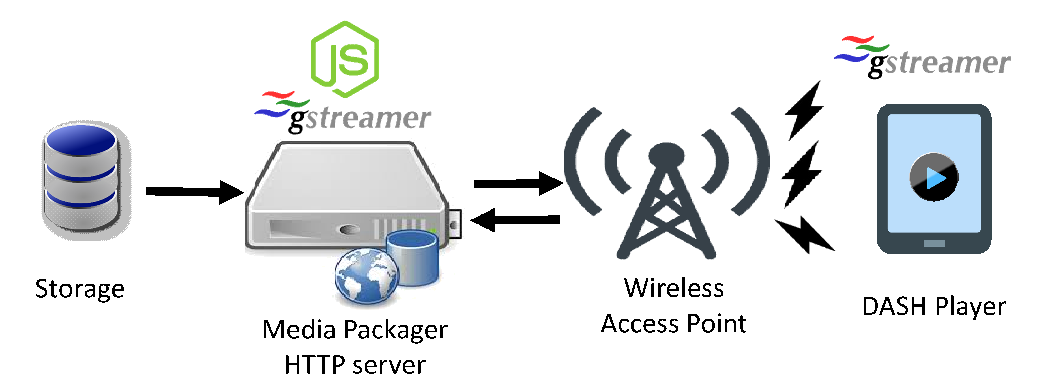
\includegraphics[width=1\textwidth,keepaspectratio]{setup.eps}
	\caption{Experimental setup.}
	\label{fig:BMSB2019setup}
\end{figure}

The Table \ref{tab:BMSB2019results} shows the results for the different fragment configurations and the employed representations in terms of the number of freezes and their average duration, and the overall latency according to the Equation (\ref{eq:BMSB2019latency}). These parameters are the common factors employed by \cite{claeys2014, hossfeld2012} for the assessment of MOS metrics.

\begin{table}[htp]
	\caption{Number of freezes (F$_{Nb}$), average freeze duration (F$_{avg}$) for each fragment configuration.}
	\centering
	\def\arraystretch{1.2}%  1 is the default, change whatever you need
	\setlength\tabcolsep{2.5pt} % default value: 6pt
	\label{tab:BMSB2019results}
	{\scriptsize
		\begin{tabular}{>{\centering\arraybackslash}m{\dimexpr0.1\textwidth-2\tabcolsep-\arrayrulewidth\relax}
				>{\centering\arraybackslash}m{\dimexpr0.1\textwidth-2\tabcolsep-\arrayrulewidth\relax}
				>{\centering\arraybackslash}m{\dimexpr0.1\textwidth-2\tabcolsep-\arrayrulewidth\relax}
				>{\centering\arraybackslash}m{\dimexpr0.1\textwidth-2\tabcolsep-\arrayrulewidth\relax}
				>{\centering\arraybackslash}m{\dimexpr0.1\textwidth-2\tabcolsep-\arrayrulewidth\relax}
			}
			\toprule
			\textbf{Conf.} & \textbf{Rep.} & \textbf{F$_{\textbf{Nb}}$} & \textbf{F$_{\textbf{avg}}$} & \textbf{Latency}\\
			\textbf{ID} & \textbf{index} & & \textbf{(ms)} & \textbf{(ms)} \\
			\midrule
			\midrule
			F$_1$ & 1 & 34 & 423 & 117\\
			F$_1$ & 2 & 35 & 410 & 124\\
			F$_1$ & 3 & 38 & 401 & 116\\
			F$_1$ & 4 & 30 & 466 & 117\\
			F$_1$ & 5 & 31 & 434 & 120\\
			F$_1$ & 6 & 13 & 445 & 126\\
			\bottomrule
			\bottomrule
		\end{tabular}
		\begin{tabular}{>{\centering\arraybackslash}m{\dimexpr0.1\textwidth-2\tabcolsep-\arrayrulewidth\relax}
			>{\centering\arraybackslash}m{\dimexpr0.1\textwidth-2\tabcolsep-\arrayrulewidth\relax}
			>{\centering\arraybackslash}m{\dimexpr0.1\textwidth-2\tabcolsep-\arrayrulewidth\relax}
			>{\centering\arraybackslash}m{\dimexpr0.1\textwidth-2\tabcolsep-\arrayrulewidth\relax}
			>{\centering\arraybackslash}m{\dimexpr0.1\textwidth-2\tabcolsep-\arrayrulewidth\relax}
		}
		\toprule
		\textbf{Conf.} & \textbf{Rep.} & \textbf{F$_{\textbf{Nb}}$} & \textbf{F$_{\textbf{avg}}$} & \textbf{Latency}\\
		\textbf{ID} & \textbf{index} & & \textbf{(ms)} & \textbf{(ms)} \\
		\midrule
		\midrule
		F$_3$ & 1 & 9 & 300 & 184\\
		F$_3$ & 2 & 3 & 492 & 187\\
		F$_3$ & 3 & 4 & 332 & 186\\
		F$_3$ & 4 & 9 & 294 & 186\\
		F$_3$ & 5 & 6 & 346 & 198\\
		F$_3$ & 6 & 11 & 401 & 222\\
		\bottomrule
		\bottomrule
		\end{tabular}
		\begin{tabular}{>{\centering\arraybackslash}m{\dimexpr0.1\textwidth-2\tabcolsep-\arrayrulewidth\relax}
			>{\centering\arraybackslash}m{\dimexpr0.1\textwidth-2\tabcolsep-\arrayrulewidth\relax}
			>{\centering\arraybackslash}m{\dimexpr0.1\textwidth-2\tabcolsep-\arrayrulewidth\relax}
			>{\centering\arraybackslash}m{\dimexpr0.1\textwidth-2\tabcolsep-\arrayrulewidth\relax}
			>{\centering\arraybackslash}m{\dimexpr0.1\textwidth-2\tabcolsep-\arrayrulewidth\relax}
		}
		\toprule
		\textbf{Conf.} & \textbf{Rep.} & \textbf{F$_{\textbf{Nb}}$} & \textbf{F$_{\textbf{avg}}$} & \textbf{Latency}\\
		\textbf{ID} & \textbf{index} & & \textbf{(ms)} & \textbf{(ms)} \\
		\midrule
		\midrule
		F$_5$ & 1 & 4 & 452 & 249\\
		F$_5$ & 2 & 14 & 312 & 256\\
		F$_5$ & 3 & 5 & 380 & 262\\
		F$_5$ & 4 & 5 & 493 & 259\\
		F$_5$ & 5 & 12 & 432 & 285\\
		F$_5$ & 6 & 13 & 430 & 317\\
		\bottomrule
		\bottomrule
		\end{tabular}
		\begin{tabular}{>{\centering\arraybackslash}m{\dimexpr0.1\textwidth-2\tabcolsep-\arrayrulewidth\relax}
			>{\centering\arraybackslash}m{\dimexpr0.1\textwidth-2\tabcolsep-\arrayrulewidth\relax}
			>{\centering\arraybackslash}m{\dimexpr0.1\textwidth-2\tabcolsep-\arrayrulewidth\relax}
			>{\centering\arraybackslash}m{\dimexpr0.1\textwidth-2\tabcolsep-\arrayrulewidth\relax}
			>{\centering\arraybackslash}m{\dimexpr0.1\textwidth-2\tabcolsep-\arrayrulewidth\relax}
		}
		\toprule
		\textbf{Conf.} & \textbf{Rep.} & \textbf{F$_{\textbf{Nb}}$} & \textbf{F$_{\textbf{avg}}$} & \textbf{Latency}\\
		\textbf{ID} & \textbf{index} & & \textbf{(ms)} & \textbf{(ms)} \\
		\midrule
		\midrule
		S & 1 & 0 & - & 2196\\
		S & 2 & 0 & - & 2231\\
		S & 3 & 0 & - & 2288\\
		S & 4 & 0 & - & 2261\\
		S & 5 & 0 & - & 2482\\
		S & 6 & 2 & 463 & 2196\\
		\bottomrule
		\bottomrule
		\end{tabular}
	}
\end{table}

It becomes clear that the reduction of the fragment duration means a reduction in latency, but it also increases the number of freezes as the network performance is not enough to deliver the fragments in time. The duration of each freeze is not related to the fragment duration as the freezes spans a duration between 300 and 400 milliseconds independently of the fragment duration. Thus, it looks like an intrinsic limit of the wireless setup. The configuration S (legacy) is the only one which is not affected by the freezes, except for the highest representation level. In any case, even when higher network resources are needed, the playout buffer is big enough to shield against any network fluctuation. As expected, the configuration F1 (1 frame per fragment) provides the lowest latency. However, the latency score is not exactly proportional to the GOP size since the latency reduction means -38\% compared to F3 (3 frames per segment) while theoretically latency should decrease 3 times. This effect is mainly produced by two factors. First, the increasing HTTP overheads when the request/response speed and volume is very high. Second, the higher data rates to be transferred due to the utilization of more keyframes meaning high bitrates and lower compression efficiency as a GOP needs to start with a keyframe to allow instant consumption of a live stream. Moreover, the number of freezes for configuration F1 is three times compared to F3 and F5 (5 frames per fragment), which means that, the maximum technical reduction of latency may significantly damage the user's QoE with higher freezes along streaming sessions.

\begin{figure}[htp]
	\centering
	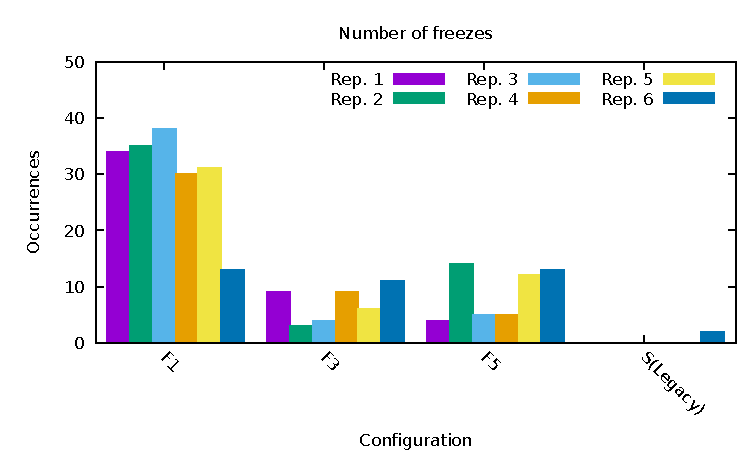
\includegraphics[width=1\textwidth,keepaspectratio]{freezes.eps}
	\caption{Number of freezes.}
	\label{fig:BMSB2019freezes}
\end{figure}

The results in terms of number of freezes along the video playback are presented in Figure \ref{fig:BMSB2019freezes}, comparing the occurrence for the different representations and fragment configurations. It is visually evident that the number of freezes is lower as the fragment duration is higher. Finally, the configuration F3 and F5 present almost the same number of freezes and duration and then F3 is preferable in order to reduce latency.

\subsection{Conclusions and Future Work}
\label{sec:BMSB2019conlusion}
This paper proposes an end-to-end system for delivery contents though a Chunked CMAF enabled MPEG-DASH live stream which aims to reduce latency, while trying to preserve major parameters of user's QoE.

The proposed solution has been integrated with Open Source MPEG-DASH framework and tested by performing experiments though a real testbed. The target of the experiments is the evaluation of the effects on user's QoE while tuning GOP and fragment duration during the Chunked CMAF packetizing in order to vary the latency of the system.

The results show that DASH players gain lower latency in any of the Chunked CMAF configuration with respects to a legacy solution but when using an aggressive configuration with a small GOP size and fragment duration the playback is frequently affected by freezes which reduce the QoE. So, to balance the latency and QoE trade-off a more conservative configuration of Chunked CMAF is suggested.


% use section* for acknowledgement
%\subsection*{Acknowledgment}






%Introduction
%\begin{savequote}[50mm]
%If our brains were simple enough for us to understand them, we'd be so simple that we couldn't.
%\qauthor{Ian Stewart }%The Collapse of Chaos: Discovering Simplicity in a Complex World
%\end{savequote}
%[Two-way complementarity of computing capabilities]
%\chapter{Two-way complementarity of computing capabilities in multi-device media services}
\chapter{Network performance forecasts for content delivery}
\chaptermark{Network performance forecasts for content delivery}
\label{chap:predictive}

\section{Context}

In the video streaming context, caching is a fundamental mechanism that aims to prevent negative effects on the QoS/QoE caused by network impairments. A CDN is a widely employed solution to cache and deliver video streams. Furthermore, it is becoming usual for CPs to employ alternative CDNs from different vendors or geographic locations to provide a more reliable service. However, the typical multi-CDN strategy is limited to selecting the CDN to be used at the start of the media session, maintaining it throughout the content playback. Then, the selected CDN is kept along all the streaming session. Moving to more dynamic solutions, that enable to switch between different CDNs when the streaming sessions are ongoing, opens lots of possibilities for optimization. Moreover, employing times series analysis to forecast network performance enables to perform proactive CDN selection and to consider the trade-off between performance (QoS) and costs (Operational Expenditure or OPEX).

Section \ref{chap:IEEETBC2020} proposes to optimize the employed CDN resources by reducing their usage to the effectively necessary moments, when delivering MPEG-DASH streams. The objective is to avoid over-provisioning of CDN resources, as it affects CP's OPEX. The proposed solution, called intelligent network flow (INFLOW), consists in a multi-CDN strategy designed to optimize CDNs utilization and reduce the resultant business costs for it. It exploits periodical MPEG-DASH media presentation description (MPD) updates to apply dynamic switching among the available CDNs at the players in a standard compliant manner. The MPD with the appropriate CDN endpoint is served by the INFLOW Media Server, which works jointly with the INFLOW Forecast Service. The INFLOW Forecast Service provides network metrics predictions based on a Long Short-Term Memory (LSTM) network, a kind of Recurrent Neural Network (RNN), when fed with the historical values of network metrics. The integration of the Forecast Server into the delivery chain allows the Media Server to serve an MPD containing the \textit{BaseURL} of the CDN, which matches target QoS and CP's business requirements. Thus, INFLOW allows for proactive and cost-effective video streaming delivery. This paper comprises the following relevant contributions:
\begin{itemize}
	\item Exploitation of network performance metrics and MPD information to apply common decisions to ongoing streaming sessions. Captured network metrics are employed to forecast CDN serving capacity (throughput) and then to select a CDN only if it would ensure the viability to serve the content at a representation bitrate from the available ones in the MPD that matches with the target minimum QoS.
	\item A dynamic approach switching from a CDN server to another depending on the performed predictions at any time. Thus, in contrast to current solutions, a streaming session is not served from a single CDN provider.
	\item Practical application of a forecast model. The literature proposing a forecast model for QoS network metrics is usually limited to theoretical analysis and simulations where the predictions are not turned into video streaming actions. On the contrary, in this work the predictions are effectively employed to switch the players among the available CDN servers, then proactively acting on the delivery.
	\item Business constraints are considered for the CDN selection. Metrics for both the OPEX and the QoS have been considered in the algorithm which selects the ideal CDN to be employed. Thus, this sophisticated approach favors the dynamic utilization of a CDN marketplace to deal with cost-effective trade-offs. The efficient utilization results in OPEX reduction, while keeping the QoS, which is a major concern for practical deployments in real-world streaming services.
	\item The evaluation includes a comparison with other CDN selection strategies in terms of QoS metrics and business cost.
\end{itemize}
The proposed solution has been implemented and validated in a distributed and heterogeneous testbed employing real network nodes and including both wired and wireless nodes. The wireless nodes were connected through a real Long-Term Evolution (LTE) network deployed with Software Defined Radio (SDR) equipment and OpenAirInterface (OAI) open-source software. The traffic demand on video players was generated according to a probability distribution widely employed in the literature. The results highlight the advantages of INFLOW for reducing the overall usage time of the available CDNs, while guaranteeing a minimum level of network bandwidth to every player.
% !TeX spellcheck = en_US
%Publications.tex
%\newcommand{\PublicationsPath}{PatentsAndPublications/Publications}

%IEEETBC2020

\section[Predictive CDN selection for video delivery based on LSTM network performance forecasts and cost-effective trade-offs]{Predictive CDN selection for video delivery based on LSTM network performance forecasts and cost-effective trade-offs}
\label{chap:IEEETBC2020}
\begin{itemize} \itemsep1pt\parskip0pt\parsep0pt
	\item \textbf{Title:} Predictive CDN selection for video delivery based on LSTM network performance forecasts and cost-effective trade-offs
	\item \textbf{Authors:} Roberto~Viola, \'Angel~Mart\'in, Javier~Morgade, Stefano~Masneri, Mikel~Zorrilla, Pablo~Angueira and Jon~Montalb\'an
	\item \textbf{Journal:} IEEE Transactions on Broadcasting
	\item \textbf{Publisher:} IEEE
	\item \textbf{Year:} 2020
	\item \textbf{DOI:}  \url{10.1109/TBC.2020.3031724}
\end{itemize}	

\textbf{Abstract:} Owing to increasing consumption of video streams and demand for higher quality content and more advanced displays, future telecommunication networks are expected to outperform current networks in terms of key performance indicators (KPIs). Currently, content delivery networks (CDNs) are used to enhance media availability and delivery performance across the Internet in a cost-effective manner. The proliferation of CDN vendors and business models allows the content provider (CP) to use multiple CDN providers simultaneously. However, extreme concurrency dynamics can affect CDN capacity, causing performance degradation and outages, while overestimated demand affects costs. 5G standardization communities envision advanced network functions executing video analytics to enhance or boost media services. Network accelerators are required to enforce CDN resilience and efficient utilization of CDN assets. In this regard, this study investigates a cost-effective service to dynamically select the CDN for each session and video segment at the Media Server, without any modification to the video streaming pipeline being required. This service performs time series forecasts by employing a Long Short-Term Memory (LSTM) network to process real time measurements coming from connected video players. This service also ensures reliable and cost-effective content delivery through proactive selection of the CDN that fits with performance and business constraints. To this end, the proposed service predicts the number of players that can be served by each CDN at each time; then, it switches the required players between CDNs to keep the (Quality of Service) QoS rates or to reduce the CP's operational expenditure (OPEX). The proposed solution is evaluated by a real server, CDNs, and players and delivering dynamic adaptive streaming over HTTP (MPEG-DASH), where clients are notified to switch to another CDN through a standard MPEG-DASH media presentation description (MPD) update mechanism.

\textbf{Keywords:} Content Delivery Network, MPEG-DASH, Operational Expenditure, Quality of Service.


\subsection{Introduction}
\label{sec:intro}

In the last few years, the demand for video content across the Internet has constantly increased. Video streams from professional applications, such as Industrial Internet of Things (IIoT), medical equipment, connected and autonomous cars, and from domestic services such as gaming, virtual reality, augmented reality, video over IP (VoIP) sports services, and  over-the-top (OTT) platforms are flooding networks with real-time data intensive sessions.

This evolution of Internet traffic makes evident the severity of the network’s capacity to guarantee a certain quality of service (QoS) for the video applications. To prevent network flooding and to make video delivery more efficient, content delivery networks (CDNs) employ geographically distributed and cost-effective infrastructures as a service (IaaS) to enhance media availability and delivery performance across the Internet. This hierarchical system that caches and stores video streams fosters efficiency while geographical locations track human daytime life cycles, which have a close relation with local content demands.

Furthermore, the current video traffic crosses networks working on a best-effort basis where the delivery time of network packets is not guaranteed. Thus, it may cause stalls during playback on player devices, damaging the quality of experience (QoE). The popularity of video streaming services over the Internet pushed video industry-Moving Picture Experts Group (MPEG)-and standardization bodies to create new formats which enable adaptive streaming over the already existing Hypertext Transfer Protocol (HTTP) infrastructures. Thus, they allow the player devices to adapt the content representation to the specific device capabilities (resolution, codecs, etc.) and the changeable network connectivity.

Dynamic Adaptive Streaming over HTTP (MPEG-DASH) \cite{sodagar2011mpeg}, which was designed to mitigate problems due to fluctuations on best-effort networks, is the solution adopted by the video industry \cite{park2017}. In fact, MPEG-DASH enables pull-based streaming \cite{begen2011} and allows for scalable distribution as it has a CDN-ready design \cite{maille2016} that enables the exploitation of existing HTTP caching infrastructures without modifications. To this end, the MPEG-DASH pipeline splits the video content into segments of fixed duration, usually between 2 and 10 seconds; then, it encodes them at different representation levels with a nominal resolution and bitrate. Thus, for each segment request, the player can switch from one representation to another depending on the assessed network status.

Nevertheless, the MPEG-DASH client-driven approach presents some drawbacks. First, each player is not aware of the existence of the others, leading to high network dynamics as the content download is not coordinated. Second, each player strives to achieve optimized individual quality, which may lead to unfairness when a congested connection path is shared \cite{akhshabi2012}. Thus, it is challenging for a content provider (CP) to ensure a certain level of quality to end users, who are accessing large volumes of content through the same access point and competing for the available bandwidth independently. Here, some issues, such as initial buffering delay, temporal interruptions, unsteady video resolution, and bitrate changes, may damage the QoE \cite{Seufert2014}.

Currently, CDNs are used to enhance media availability and delivery performance across the Internet. The proliferation of CDN vendors and business models allows the CP to use multiple CDN providers simultaneously \cite{adhikari2012}, \cite{adhikari2012-2}, \cite{adhikari2015}. However, extreme concurrency dynamics can affect CDN capacity, causing performance degradation and outages, while overestimated demand affects costs, thereby increasing the operational expenditure (OPEX) of the CP \cite{silva2020}.

Upcoming 5G networks will need advanced and intelligent mechanisms to dynamically deliver each data flow according to the required service level agreement (SLA) and considering performance costs trade-offs.
This concept is where the approach proposed by this paper takes place, fusing network characteristics and media service options to match user satisfaction and business policies.

\subsubsection{Contribution}
\label{sec:overview}

This work proposes a novel solution called intelligent network flow (INFLOW) for CDN selection in a multi-CDN delivery environment. It exploits periodical MPEG-DASH media presentation description (MPD) updates to apply dynamic switching among the available CDNs at the video players in a standard compliant manner. The MPD with the appropriate CDN endpoint is served by the INFLOW Media Server, which works jointly with the INFLOW Forecast Service. The INFLOW Forecast Service provides network metrics predictions based on a Long Short-Term Memory (LSTM) network, a kind of Recurrent Neural Network (RNN), when fed with the historical values of network metrics. The integration of the Forecast Server into the delivery chain allows the Media Server to serve an MPD containing the \textit{BaseURL} of the CDN, which fits target QoS and CP's business requirements. Thus, INFLOW allows for proactive and cost-effective video streaming delivery. 
The proposed solution comprises the following relevant contributions:
\begin{itemize}
	\item Exploitation of network performance metrics and MPD information to apply common decisions to ongoing streaming sessions. Captured network metrics are employed to forecast CDN server capacity, then select a CDN only if it would guarantee the viability to serve the content at a minimum representation bitrate from the available ones in the MPD.
	\item Dynamic CDN server switching. We employ a dynamic approach switching from a CDN server to another depending on the performed predictions at any time. Thus, in contrast to current solutions, a streaming session is not served from a single CDN provider.
	\item Practical application of a forecast model. The literature proposing a forecast model for QoS network metrics is usually limited to theoretical analysis and simulations, and the predictions are not turned into video streaming actions. On the contrary, we exploit the predictions to switch the players among the available CDN servers, then proactively act on the delivery.
	\item Business constraints are considered for the CDN selection. We include metrics for both the OPEX and the QoS in the algorithm which selects the ideal CDN to be employed. Thus, this sophisticated approach favours the dynamic utilisation of a CDN marketplace to deal with cost-effective trade-offs. OPEX reduction, while keeping the QoS, is a major concern for practical deployments in real-world streaming services.
\end{itemize}
To achieve the above contributions, we develop a Forecast Service and a Media Server as complementary parts of the proposed INFLOW solution. Forecast Service executes an LSTM network performing real-time predictions of the QoS metrics. Media Server updates the MPD according to the network metrics predictions and CP's business rules and serves it to the clients.
The solution was integrated and tested in a real setup employing a multi-modal testbed including both wired and wireless nodes. The wireless nodes were connected through a real Long-Term Evolution (LTE) RAN infrastructure of an operational Mobile Network stack including the radio base station (eNodeB) and the Evolved Packet Core (EPC). The traffic demand on video players was generated according to a probability distribution widely employed in the literature.

The paper is structured as follows. First, section \ref{sec:sota} reviews related work in the field of video delivery based on CDN performance and network traffic generation and forecast. Then, section \ref{sec:system} introduces the proposed INFLOW server, a novel media server equipped with a forecast service that tunes the delivery and applies a CDN selection mechanism based on QoS metrics and business rules, as the main focus of the article. Section \ref{sec:setup} describes the implemented setup using a real testbed, while section \ref{sec:validation} presents the results of the validation experiments. Finally, we assert our conclusions and future work in section \ref{sec:conclusion}.


\subsection{Related Work}
\label{sec:sota}

\textbf{\subsubsection{CDN resource selection}
	\label{sec:cdnselection}}

A CDN is a network function widely employed to improve content delivery by means of cloud service provisioning cache features. Fueled by the CDN vendor proliferation, media platforms exploit multi-CDN strategies to obtain more reliable content delivery that provides a steadier QoS and higher customer satisfaction. Nevertheless, the CDN selection criteria can be different for any CP.

A widely employed solution applies a static selection made by the media server when a new streaming session starts. This is used by Netflix \cite{adhikari2012} and Hulu \cite{adhikari2012-2}, with big similarities \cite{adhikari2015}. They use three different CDN vendors mapping CDNs to the location of client device or to a subscriber. Moreover, they evidence that, the selected CDN is fixed during the streaming session even when the QoS degrades. Thus, providers are more prone to lower the representation bitrate instead of operating alternative CDNs. Hence, the authors conjecture that CDN selection is most likely based on business policies.

However, Netflix has changed its strategy over the years, and nowadays it uses its own CDN, which is called Open Connect \cite{botteger2018}. Open Connect can be run inside the ISP infrastructure so that a better QoS can be achieved as the content is closer to the user. Netflix’ solution is not that different from the open CDN architecture proposed by \cite{zhang2014}. The authors propose collaborative participation of CPs and ISPs. On one hand, cost reductions are realized as the ISP acts as a CDN. On the other hand, the ISP provides better performance to the clients and reduces traffic as the content is already present in its network infrastructure.

The awareness of end-to-end QoS metrics measured by the client can make the difference when the employed CDN is dynamically chosen by the clients. The authors of \cite{otto2012} propose a client-side CDN selection. As a drawback, client-side strategies do not produce a coordinated decision as each client analyses the network performance of each CDN independently, introducing bias and communication overheads. Hence, a client-side CDN selection is not an optimal solution.

An intermediate solution consists of Domain Name System (DNS) resolution. Here, the DNS server can resolve a fixed hostname owned by the CP into different IP addresses of several CDNs. Depending on the DNS resolution, the client is directed to an appropriate CDN. The YouTube DNS-based solution is shown in \cite{torres2011}. YouTube goes further as it allows for the use of a hybrid DNS and application-level CDN selection. First, the DNS redirects the client to a server. Then, the server accepts or reject the client depending on the workload. If the client is refused, the DNS redirects the client to another server.

In \cite{goel2015}, the effects of DNS resolution for CDN selection are further studied. The authors conclude that, depending on the DNS service provider, Akamai and Google CDN servers are chosen differently. Consequently, CDN performance highly depends on the load balancing rules of the DNS server. Here, a suboptimal CDN server selection leads to a higher round-trip delay time (RTT). To solve this problem, the authors propose a DNS-proxy running on the client. This proxy forwards the DNS requests to different DNS servers; then, it compares the responses to identify the best performing CDN server. However, these solutions are loosely coupled from media player requests slots applying balancing policies independently of media player timing. Instead, out approach is triggered by the requests with the most recent available information.

CDN Brokering \cite{biliris2002} is the ability to redirect clients dynamically among two or more CDNs. CDN brokers collect and analyze the performance metrics of the available CDNs to select the one that performs best. Their work, in contrast to traditional multi-CDN strategies, is not limited to the selection of the initial CDN for each client. This solution also moves clients between CDNs when performance degradation is detected in real time. Thus, the CDN is dynamically and seamlessly changed. As an example, the European Broadcasting Union (EBU) proposed the EBU Flow Multi-CDN \cite{EurovisionFLOW}, which consists of a CDN switching service that selects the optimal CDN at any time. Similar approaches are provided by Citrix \cite{citrix2} and LightFlow \cite{lightflow}. Thus, these solutions are usually provided by intermediaries, federating infrastructures from different vendors. However, our approach keeps the control to the media service manager able to dynamically change the business policy or tune the cost function.

Edge computing systems promise a revolution on smart delivery of media traffic fueled by Multi-access Edge Computing (MEC) \cite{etsi2019} architectures from 5G.
Thus, new solutions for improving multi-CDN delivery involve investigating MEC services. In \cite{viola2018} a MEC proxy is proposed. The proxy can retrieve video streaming metrics of video players at the access point transparently and CDNs performance metrics from the wired link. Compared to a pure client-decision, a MEC proxy can evaluate the performance of each CDN just once and apply conclusions to other sessions (independently from the number of connected players). Moreover, it empowers the delivery through a local edge cache. This feature guarantees traffic reduction compared to server-side CDN selection as recurrent content can be downloaded and cached once for every client. In \cite{carrozzo2018}, a similar solution for a MEC-based cache is proposed.
However, till the moment the edge systems realize, current CDN infrastructures makes the difference, and universal solutions that dynamically manage balancing are required.

In \cite{frank2013}, a prototype of CDN and ISP collaboration is proposed. The ISP provides the CDN provider with services that allow the CDN provider to retrieve geographical user distribution and allocate server resources inside the ISP's network topology. The authors of \cite{wichtlhuber2015} propose a similar solution without the binding to allocate resources in the ISP's infrastructure. In this case, a redirection center inside the ISP's network intercepts the client’s requests and selects the appropriate CDN. This process is transparent to the client as the redirection center stores the content in a CDN surrogate and instructs an OpenFlow controller to migrate the traffic to a CDN surrogate.

Contrary to those approaches provisioning or balancing serving resources, other works focus on the selection of the appropriate bitrate to avoid congestion for a static number of servers \cite{sadi2020} or network assets \cite{giannone2020}. To this end, the MPD is parsed and heavier options are cropped. As implemented in these works, our approach employs a compliant MPD update mechanism. But, in our case, it is exploited to dynamically manage the CDN resources at any moment depending on network performance forecasts and CP business rules. The CP can tune the media server, thereby influencing CDN selection when the video player requests an MPD update.

\subsubsection{Time series for network traffic forecast}
\label{sec:timeseries}

\begin{table}[t]
	\caption{Forecast models comparison}
	\centering
	\label{tab:IEEETBC2020models}
	\def\arraystretch{1.2}%  1 is the default, change whatever you need
	\setlength\tabcolsep{2.0pt} % default value: 6pt
	{\scriptsize
	\begin{tabular}{>{\centering\arraybackslash}m{\dimexpr0.2\textwidth-2\tabcolsep-\arrayrulewidth\relax}
			>{\centering\arraybackslash}m{\dimexpr0.15\textwidth-2\tabcolsep-\arrayrulewidth\relax}
			>{\centering\arraybackslash}m{\dimexpr0.15\textwidth-2\tabcolsep-\arrayrulewidth\relax}
			>{\centering\arraybackslash}m{\dimexpr0.5\textwidth-2\tabcolsep-\arrayrulewidth\relax}
		}
		\toprule
		\textbf{Model} & \textbf{Approach} & \textbf{Number of variables} & \textbf{Internal parameters}\\
		\midrule
		\midrule
		ARIMA & statistical & univariate & a-priori (regression, integration and moving average parameters)\\
		Exponential smoothing & statistical & univariate & a-priori (smoothing factor)\\
		SETARMA & statistical & univariate & a-priori (regression, moving average and threshold delay parameters)\\
		GARCH & statistical & univariate & a-priori (regression and lag length parameters)\\
		Feed-forward NN & neural network & multivariate & trained (weight and bias)\\
		RNN & neural network & multivariate & trained (input, output and forget factors)\\
		LSTM & neural network & multivariate & trained (input, output and forget factors)\\
		\bottomrule
		\bottomrule
	\end{tabular}
	}
\end{table}

The goal of applying time series analysis to network traffic data is to forecast future conditions to take actions proactively when actuation performance or cost policies are satisfied. These techniques allow network management systems to prevent network under-performance and outages, thereby addressing network congestion preemptively.

The auto-regressive integrated moving average (ARIMA) is employed in \cite{calheiros2014} to predict the workload of cloud services. It employs historical records of observed requests to predict the volume of requests for the following time interval. The results reveal that the model can obtain the general trend, but it lacks the ability to accurately and timely track traffic peaks. The authors of \cite{dong2015} apply both ARIMA and exponential smoothing models to predict throughput in an LTE network. The two models are complementary, with ARIMA outperforming the exponential smoothing models on weekdays and the exponential smoothing models outperforming ARIMA on weekends.

The authors of \cite{amin2012} and \cite{amin2012-2} found limitations in ARIMA while modelling QoS attributes. QoS attributes such as bandwidth or latency have nonlinear behaviors that do not fit the linear assumption of the ARIMA model. They overcame this by introducing hybrid linear and non-linear models. The linear model was represented by the ARIMA model. For the non-linear model, \cite{amin2012} used the self-exciting threshold autoregressive moving average (SETARMA) model, while \cite{amin2012-2} employed a generalized autoregressive conditional heteroscedastic (GARCH) model. In both cases, the proposed solution outperforms a standalone ARIMA model in forecasting the time between QoS violations.

In recent years, machine learning (ML)-based techniques for time series prediction have exhibited satisfactory performances. Specifically, neural networks (NNs) are gaining adoption in the generation of time series models. The authors of \cite{zadeh2010} propose a feed-forward NN for predicting the execution time of services while varying the number of requesters. In \cite{belhaj2009}, a recurrent NN (RNN) is employed to forecast the end-to-end delay from RTT metrics.

In \cite{trinh2018}, an LSTM model, a particular type of RNN, was proposed. The authors employed a multivariate time series model where data input was probed from downlink control information (DCI) messages, such as resource blocks, transport block size, and scheduling information.

Table \ref{tab:IEEETBC2020models} shows the main differences between the employed techniques for time series forecasting. Clearly, NN-based approaches have the advantage to employ several variables as input and/or output of the models, while statistical ones are limited to one. Moreover, statistical approaches need a-priori evaluation of internal parameters, while NN-based ones are trained through a dataset of previous collected metrics. Here, the parameters for statistical approaches are intended for the whole model, while for NN-based ones, parameters must be trained for each internal cell.

From the available algorithms to analyze and predict time series, we employ LSTM network model as it satisfies two requirements. First, in terms of accuracy, statistical solutions (ARIMA and its derivatives) are slow when tracking quick fluctuations in time series as they tend to concentrate on the average value of the past observed values, as revealed in \cite{wang2017}. Second, in terms of multivariate time series, statistical solutions only can predict one variable. Thus, ARIMA would require separate models for forecasting both latency and bandwidth. On the contrary, LSTM is ready to process multivariate time series. The authors of \cite{azari2019} and \cite{azari2019-2} revealed that, the higher the number of input variables, the better the traffic predictions of LSTM when compared to ARIMA.

% needed in second column of first page if using \IEEEpubid
%\IEEEpubidadjcol

\subsection{INFLOW solution}
\label{sec:system}

\subsubsection{System architecture}
\label{sec:detailedcontribution}

To achieve reliable and cost-effective video delivery, we propose the inclusion of our INFLOW solution in the video delivery chain. The overall scenario of the solution is depicted in Figure \ref{fig:IEEETBC2020scenario}. The INFLOW solution is composed of two components:
\begin{itemize}
	\item INFLOW Forecast Service: it receives the QoS performance metrics from the video players and processes them to predict the QoS values in the future.
	\item INFLOW Media Server: it exploits the results provided by the Forecast Service by combining them with the CP's business rules to select the appropriate CDN for each client.
\end{itemize}

\begin{figure}[htp]
	\centering
	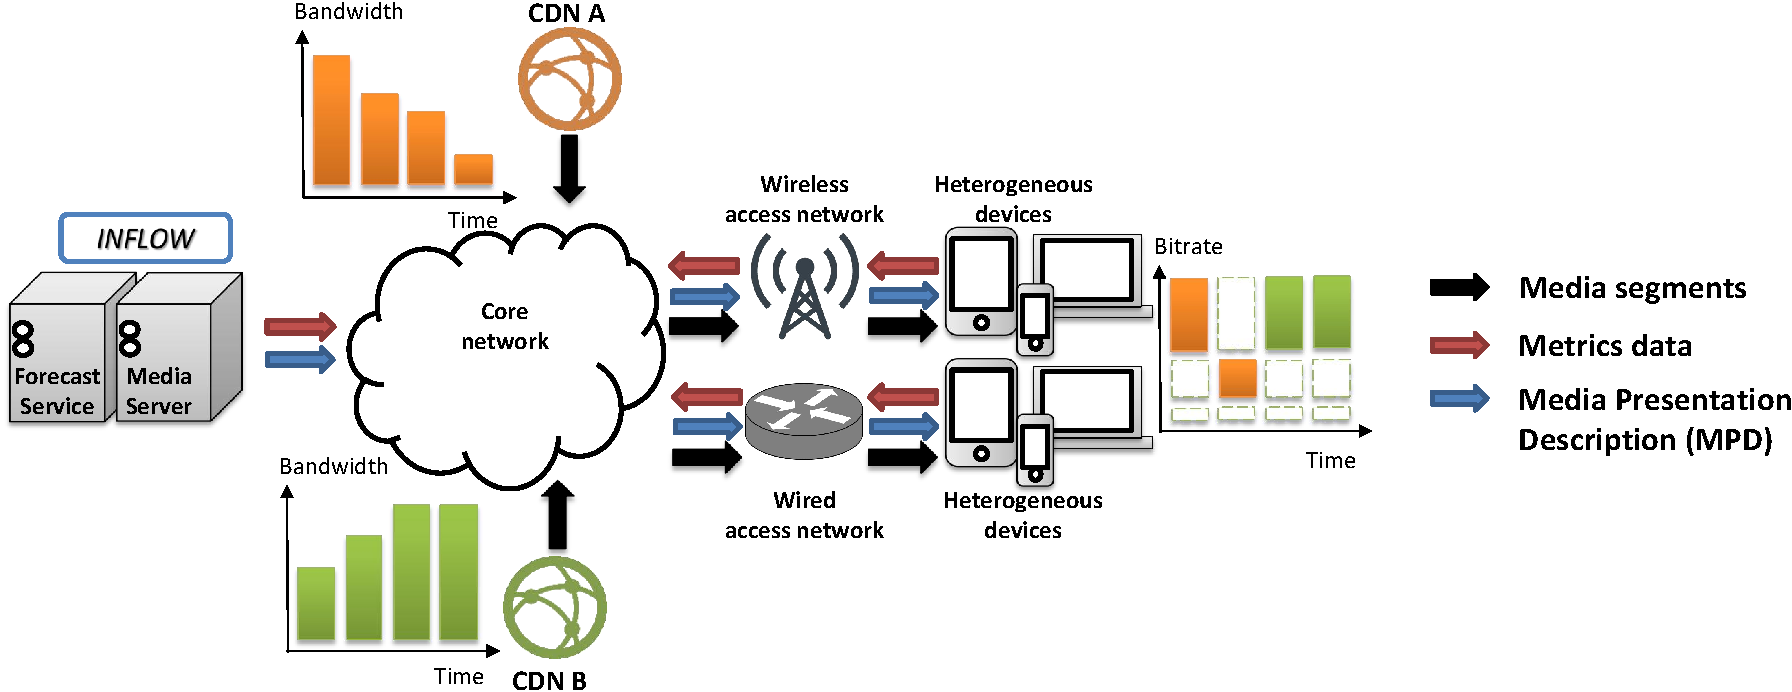
\includegraphics[width=1\textwidth,keepaspectratio]{system.pdf}
	\caption{General scenario of the proposed solution.}
	\label{fig:IEEETBC2020scenario}
\end{figure}

Owing to the utilization of MPEG-DASH, INFLOW includes the following features:
\begin{itemize}
	\item Scalability. New CDNs can be easily managed by adding them to the initial MPD.
	\item Real-time migration of video players to CDN providers. Supported by standard-compliant MPEG-DASH MPD update mechanism manages the utilization of a CDN by the video player according to the gathered metrics and business policies.
	\item MPDs can be parsed and processed even when the content is encrypted with the MPEG-DASH Common Encryption Scheme (CENC) \cite{isocenc}. The CENC format encrypts the media segments indexed in the MPD, but the MPD is not encrypted.
\end{itemize}

The sequence diagram of the exchanged messages is depicted in Figure \ref{fig:IEEETBC2020seqdiag2}. Media segments are stored at different CDNs, while the MPD is served by the INFLOW Media Server. It is important that the media server uses a dynamic MPD as it forces the player to periodically update, overwriting the Minimum Update Period attribute from the MPEG-DASH standard \cite{lohmar2011}. On the other side, each video player downloads the initial MPD and starts requesting for segments from the initial CDN. A client-side adaptation mechanism constantly monitors the statistics of the downloaded segments to select a representation level among those available that fits with the experienced network performance. Thus, the video player aims to prevent stalls during playback. Typical monitored metrics are the network bandwidth and latency, which provide a direct measure of the QoS experienced by the client. Moreover, these measurements are sent to the INFLOW forecast service. Thus, video player should support a mechanism for sending feedback to the forecast service, such as Server and Network-assisted DASH (SAND) standard \cite{thomas2016}. Finally, INFLOW forecast service stores the measurements and uses them to predict the future values.

\begin{figure}[htp]
	\centering
	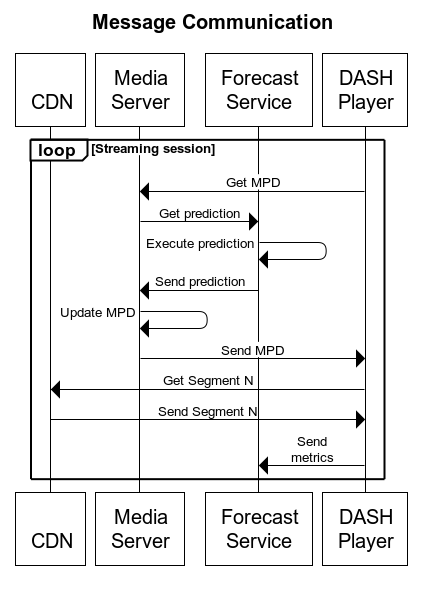
\includegraphics[width=0.65\textwidth,keepaspectratio]{communication.png}
	\caption{Sequence diagram of the INFLOW solution for video delivery.}
	\label{fig:IEEETBC2020seqdiag2}
\end{figure}

The MPD served by the media server is fully conditioned by the prediction of the forecast service. Every time a player requests an updated version of the MPD, the media server retrieves a prediction from the forecast service and decides to serve the current MPD or to change the CDN included. Therefore, the forecast service does not apply any QoS or business rules—it simply processes the information provided by the players. The QoS and business-based decisions are made by the media server, and this decision process is executed in real-time as the predictions are rendered out of date after the predicted interval, leading to a new decision. Therefore, the shorter is the segment duration, the more immediate is the forecast validity and the prompter is the MPD update.

The QoS forecasts serve two roles. First, the INFLOW Media Server can select an appropriate CDN to shield from CDN service degradation and outages based on the most recent detected performance. To this end, the server receives alternative CDNs from the initial MPD and replaces the \textit{BaseURL} tag in the MPD with another CDN endpoint to migrate a client. Second, the media server can count the video sessions served by each CDN. On top of this information, the media server can apply cost-effective policies, allocating extra CDN resources to enforce QoS or retiring CDN assets to reduce the number of employed CDN servers. Thus, the media service can manipulate the OPEX ranges to meet the business model.

In the following section, we describe separately the two components of the INFLOW solution.

\subsubsection{INFLOW Forecast Service}
\label{sec:forecastservice}

The INFLOW forecast service is in charge of collecting network metrics probed and sent by the video players and processing them to predict the values in future slots. The most recent metrics are processed while older ones are discarded using a sliding window mechanism. The decision program of the forecast service is shown in Algorithm \ref{alg:IEEETBC2020algorithmForecast}.

\begin{algorithm}
	\renewcommand{\algorithmicrequire}{\textbf{Input:}}
	\renewcommand{\algorithmicensure}{\textbf{Output:}}
	\caption{INFLOW Forecast Service}
	\label{alg:IEEETBC2020algorithmForecast}
	\begin{algorithmic}
		\Function{predictMetrics}{$\overline{bw_{t-1}^{k}}$, $\overline{l_{t-1}^{k}}$, $CDN^{k}$}
		\State \Comment{for each CDN infrastructure}
		\Require $\overline{bw_{t-1}^{k}}$ \Comment{\parbox[t]{.5\linewidth}{bandwidth mean for the \linebreak most recent period @$CDN^{k}$}}
		\Require $\overline{l_{t-1}^{k}}$ \Comment{\parbox[t]{.5\linewidth}{latency mean for the \linebreak most recent period @$CDN^{k}$}}
		\Ensure $\widehat{{bw}_{t}^{k}}$ \Comment{bandwidth prediction}
		\Ensure $\widehat{{l}_{t}^{k}}$ \Comment{latency prediction}
		\State $\{bw^{k}\}$ = \{$\overline{bw_{t-1}^{k}}$,...,$\overline{bw_{t-N}^{k}}$\} \Comment{N bandwidth samples}
		\State $\{l^{k}\}$ = \{$\overline{l_{t-1}^{k}}$,...,$\overline{l_{t-N}^{k}}$\} \Comment{N latency samples}
		\State $\widehat{{bw}_{t}^{k}}$,$\widehat{{l}_{t}^{k}}$ $\leftarrow$ LSTM(\{$bw^{k}$\},\{$l^{k}$\}) \Comment{\parbox[t]{.28\linewidth}{update forecast model $CDN^{k}$}}
		\EndFunction
	\end{algorithmic}
\end{algorithm}

The input are the last \textit{N} historical values of network bandwidth and latency measured and reported by the players for a specific CDN ($CDN^{k}$). The samples comprised in the most recent period are captured during last segment download. The video player requests segments in a regular pace to fill its buffer, according to the media duration of the segment. In total, the algorithm processes two variables taken in \textit{N} time instants. Every new sample should be taken at a fixed temporal distance from the previous one. Nevertheless, this assumption of equal distance among the samples is not guaranteed as players usually run asynchronously, and then the reports are sent in a random time inside a segment slot. To overcome this problem, the INFLOW forecast server employs a mean value of samples within a second as the input of the algorithm (\{$\overline{bw_{t-1}^{k}}$,...,$\overline{bw_{t-N}^{k}}$\} and \{$\overline{l_{t-1}^{k}}$,...,$\overline{l_{t-N}^{k}}$\}). The input is processed through the LSTM network to predict the values in the next second ($\widehat{{bw}_{t}^{k}}$ and $\widehat{{l}_{t}^{k}}$). The predicted values are the output of the algorithm.

It is important to underline that the benefits of an LSTM network over statistical approaches are two-fold. First, the LSTM network performs better when time series includes quick fluctuations \cite{wang2017}. Second, it is valid for multivariate time series, such as bandwidth and latency, where statistical methods fail to simultaneously process several components \cite{azari2019}, \cite{azari2019-2}.

\subsubsection{INFLOW Media Server}
\label{sec:mediaserver}

The media server must serve the MPD of the video players to provide awareness on available representations, content formats and metadata, and CDN endpoints. In our case, as we were interested in CDN localization, the served MPD could include one or more \textit{BaseURL} tags containing the URLs of the CDN servers. In cases with only one \textit{BaseURL}, the client is forced to use it.

The INFLOW media server stores an initial MPD containing different \textit{BaseURL} tags and modifies it while excluding CDN alternatives to force a CDN to perform according to the algorithm outcomes, which exploits the predictions provided by the INFLOW forecast service. The decision program of the media server is shown in Algorithm \ref{alg:IEEETBC2020algorithmServer}.

\begin{algorithm}
	\renewcommand{\algorithmicrequire}{\textbf{Input:}}
	\renewcommand{\algorithmicensure}{\textbf{Output:}}
	\caption{INFLOW Media Server}
	\label{alg:IEEETBC2020algorithmServer}
	\begin{algorithmic}
		\Function{updateMPD}{$urlMPD$, $SLA$}
		\State \Comment{for each MPD request}
		\Require $urlMPD$ \Comment{requested MPD}
		\Require $SLA$ \Comment{applicable SLA}
		\Ensure $MPD$ \Comment{updated MPD}
		\State $MPD$ $\leftarrow$ initial($urlMPD$) \Comment{requested MPD file}
		\State $bw_{min}$ $\leftarrow$ targetQoS($SLA$) \Comment{\parbox[t]{.35\linewidth}{minimum bandwidth per player}}
		\State $d_{s}$ $\leftarrow$ $MPD$ \Comment{segment duration}
		\State \{$CDN_{list}$\} $\leftarrow$ $MPD$ \Comment{set of alternative CDNs}
		\ForAll { ${CDN}^{k}$ $\in$ \{$CDN_{list}$\} } \Comment{for each CDN}
		\State $\overline{bw_{t-1}^{k}}$ $\leftarrow$ mean(\{$bw_{[t-1,t)}^{k}$\}) \Comment{\parbox[t]{.33\linewidth}{average for most recent period @ $CDN^{k}$}}
		\State $\overline{l_{t-1}^{k}}$ $\leftarrow$ mean(\{$l_{[t-1,t)}^{k}$\})  \Comment{\parbox[t]{.33\linewidth}{average for most recent period @ $CDN^{k}$}}
		\State {$\widehat{{bw}_{t}^{k}}$,$\widehat{{l}_{t}^{k}}$} $\leftarrow$ predictMetrics($\overline{bw_{t-1}^{k}}$,$\overline{l_{t-1}^{k}}$,$CDN^{k}$)
		\State $n^{k}$ $\leftarrow$ sessions($CDN^{k}$) \Comment{total $CDN^{k}$ sessions}
		\State $\widehat{n^{k}}$ $\leftarrow$ policy($\widehat{{bw}_{t}^{k}}$,$\widehat{{l}_{t}^{k}}$,$n^{k}$,$bw_{min}$,$d_{s}$,$CDN^{k}$)
		\State \Comment{$CDN^{k}$ capacity}
		\If {($\widehat{n^{k}}$ $>$ $n^{k}$)} \Comment{$CDN^{k}$ admits more sessions}
		\State $BaseURL$ $\leftarrow$ URL($CDN^{k}$)
		\State \Comment{write $CDN^{k}$ URL}
		\State $MPD$ $\leftarrow$ update($MPD$,$BaseURL$)
		\State \Comment{update MPD}
		\EndIf
		\EndFor
		\EndFunction
	\end{algorithmic}
\end{algorithm}

The algorithm takes an initial configuration of minimum bandwidth to be provided to the clients ($bw_{min}$) according to the SLA, and the initial MPD. From the MPD, it retrieves the segment duration ($d_{s}$) and a list of the CDNs (\{$CDN_{list}$\}). When an MPD request reaches the media server, it selects an appropriate CDN ($CDN^{k}$) from the CDN list. This list (\{$CDN_{list}$\}) is ordered in ascending order according to expenses. Thus, the media server first employs the affordable providers, migrating users to cheaper services when possible. The media server retrieves the prediction for each CDN from the forecast service ($\widehat{{bw}_{t}^{k}}$ and $\widehat{{l}_{t}^{k}}$) and stops if the expected capacity ($\widehat{n^{k}}$) is higher than the current ones ($n^{k}$). In other words, it selects the most affordable CDN that has the capacity to serve more players. The number of expected players is evaluated through the predictions and the initial configuration by means of Equation \ref{eq:IEEETBC2020players}.

\begin{equation}
\label{eq:IEEETBC2020players}
\widehat{n^{k}} = \frac{(d_{s}-\widehat{{l}_{t}^{k}})*\widehat{{bw}_{t}^{k}}*n^{k}}{d_{s}*bw_{min}}
\end{equation}

To be timely delivered, the theoretical maximum download time of a segment should be lower than the segment duration. Furthermore, a padding time must be considered to take into account the delay introduced by the network during the transmission. Consequently, the predicted latency ($\widehat{{l}_{t}^{k}}$) is used as a penalization factor to estimate the effective download time ($d_{s}$-$\widehat{{l}_{t}^{k}}$). Then, this value is multiplied by the predicted average bandwidth per video player ($\widehat{{bw}_{t}^{k}}$) to assess the average volume of data that each player can download. The total data capacity is obtained by multiplying the number of sessions in the CDN ($n^{k}$) by the average volume of data that each player can download. Finally, the overall traffic demand is divided by the amount of data that a player should download during a segment duration ($d_{s}$) according to the SLA using the minimum bandwidth provided ($bw_{min}$). The final value is the CDN capacity according to an SLA, which is indicative of the number of video streaming sessions that the CDN can serve ($\widehat{n^{k}}$).

Once a CDN is assigned to a session, the media server selects the \textit{BaseURL} corresponding to the CDN and generates a new MPD by modifying the initial one. The order of the CDNs in the list is important as they are ranked depending on the cost. Thus, the media server chooses the first CDN that fits with the necessary resources; then, the most affordable ones are quickly booked to reduce CP's OPEX.

\subsection{Testbed setup}
\label{sec:setup}

To demonstrate the cost-effective advantages of the INFLOW approach in terms of QoS enforcement and CP's OPEX reduction, we deployed a heterogeneous and distributed setup employing both FED4FIRE+ facilities \cite{nussbaum2019} and our facilities at Vicomtech (San Sebastián, Spain). Fed4FIRE+ is a Horizon 2020 project that provides open and accessible testbeds to support research and innovation initiatives in Europe. Among the available facilities, we employed NITOS's network infrastructure \cite{makris2015} at University of Thessaly's campus (Volos, Greece). NITOS provides heterogeneous testbeds to execute experiments on real wired and wireless networks.

We use D-DASH dataset and infrastructure \cite{lederer2013}, with Dynamic Adaptive Streaming over HTTP (DASH) standard content mirrored over different sites at different locations to perform CDN-based scientific evaluations.
The dataset includes the Red Bull Playstreet video sequence, which is owned by Red Bull Media House and licensed for scientific purposes. This sequence is encoded for 17 video representations through advanced video coding (H.264/AVC) and 4 dual channel audio representations through advanced audio coding (AAC). Both audio and video are segmented with different segment lengths of 2, 4, 6, 10, and 15 seconds, and multiplexed in ISO MPEG4 files (ISO/IEC 14496-12 - MPEG-4 Part 12). For our experiments, we employed 2 seconds segments to focus on live video content where dense client cells and congestion of CDNs were likely. We did not modify the video representations; instead, we used the available representations in the dataset. The representations range from a resolution of 320 x 240 and 30 fps at 100 kbps to a resolution of 1920 x 1080 and 30 fps at 6000 kbps. As the client-side bitrate adaptation mechanism works on a best-effort basis and do not take care of the presence of other connected players, each player struggles to achieve the highest representation bitrate.

The final experimental setup comprises the following:
\begin{itemize}
	\item 4 UE nodes: client nodes located at NITOS and running 100 DASH video players based on GStreamer multimedia framework \cite{gstreamer}. They feature both Ethernet and LTE interfaces and are placed in the isolated environment of the NITOS indoor testbed where they form a grid topology.
	\item 1 eNodeB: USRP provided node performing eNodeB stack located at NITOS. It forwards the packets from the clients to the Access and Core Network.
	\item 1 EPC node: wired node close to the eNodeB that executes the EPC stack.
	\item 1 INFLOW Media Server: node at Vicomtech based on a virtual machine with 2 GB RAM and single-core CPU. It is provided with a public IP address to serve the MPD to the video players. It runs a Node.js \cite{nodejs} server application which applies QoS and CP's business rules when sending the MPD to the client.
	\item 1 INFLOW Forecast Service: node at Vicomtech based on a physical machine having 12 GB RAM and quad-core Intel i5 6500 CPU. To perform predictions, it features NVIDIA GTX 1050 TI executing the LSTM model based on TensorFlow \cite{tensorflow}.
	\item 3 servers: they belong to the D-DASH dataset \cite{lederer2013} providing alternative CDNs storing the media segments to perform CDN-based scientific evaluations. They are located at different sites with different nominal performances in terms of bandwidth and latency.
\end{itemize}

To distribute the video streaming sessions between the wired and LTE network interfaces, we considered the last Cisco report concluding that mobile traffic covers 9\% of the total IP video traffic \cite{ciscovideo2017}. Hence, the experiment setup includes nine video players connected through the LTE interface and 91 players employing Ethernet interface. The use of different access networks is helpful for demonstrating its applicability in representative and multi-modal scenarios. Moreover, we modeled player inter-arrival rate and session duration according to \cite{yu2006}, which provides an extensive analysis on user behavior while accessing streaming services. Thus, the inter-arrival time distribution is a modified version of the Poisson distribution, while the session duration follows the declared sections of 5 (37.44\%), 10 (52.55\%), or 25 min (75.25\%).

During the experiment, a preliminary step was performed to generate a QoS performance metric dataset for training our LSTM model at the Forecast Service. The setup for dataset creation is depicted in Figure \ref{fig:IEEETBC2020dataset}. Here, the Media Server serves a static MPD. It does not allow for player migration among the different CDNs so that full characterization of a specific CDN can be achieved, resulting in a time series for a CDN. Then, during streaming sessions, network bandwidth and latency measurements provided by the video players are stored in an Elasticsearch \cite{gormley2015} database and employed to train the forecast service predictor. Optionally, Kibana \cite{gupta2015-2} dashboards are available to visualize the collected metrics and guide LSTM training and tuning.

\begin{figure}[htp]
	\centering
	\subfloat[]{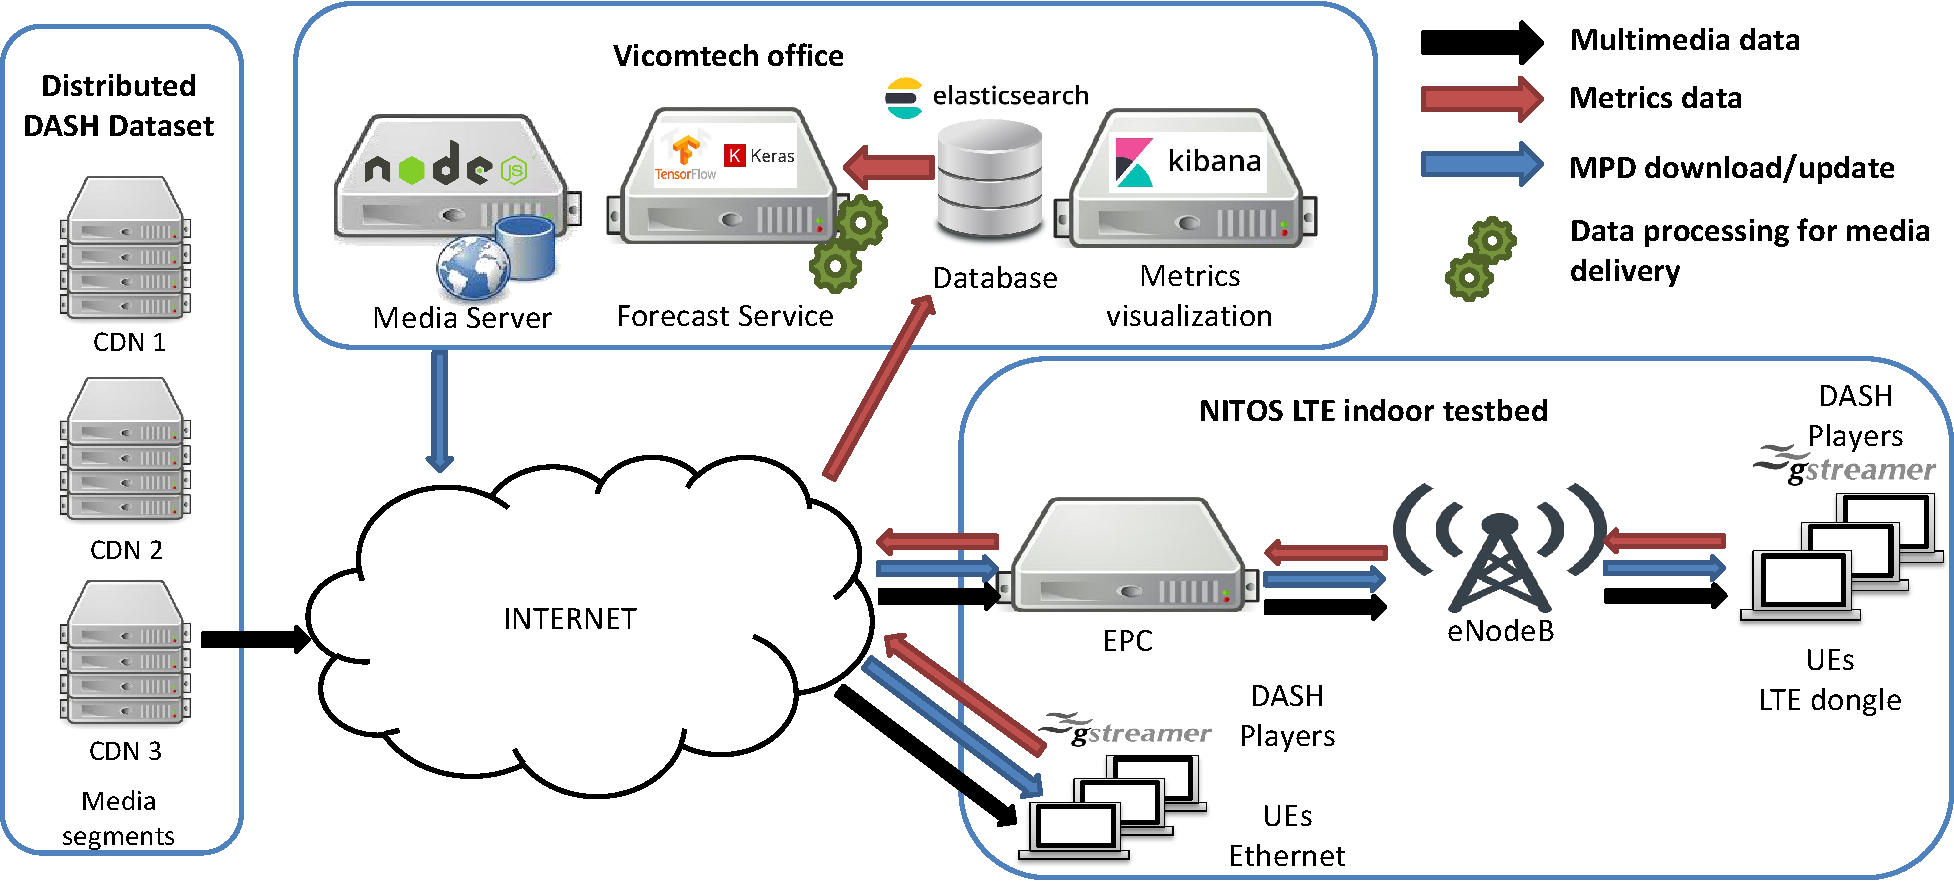
\includegraphics[width=1\textwidth,clip,keepaspectratio]{training.pdf}%
		\label{fig:IEEETBC2020dataset}}
	\hfil
	\subfloat[]{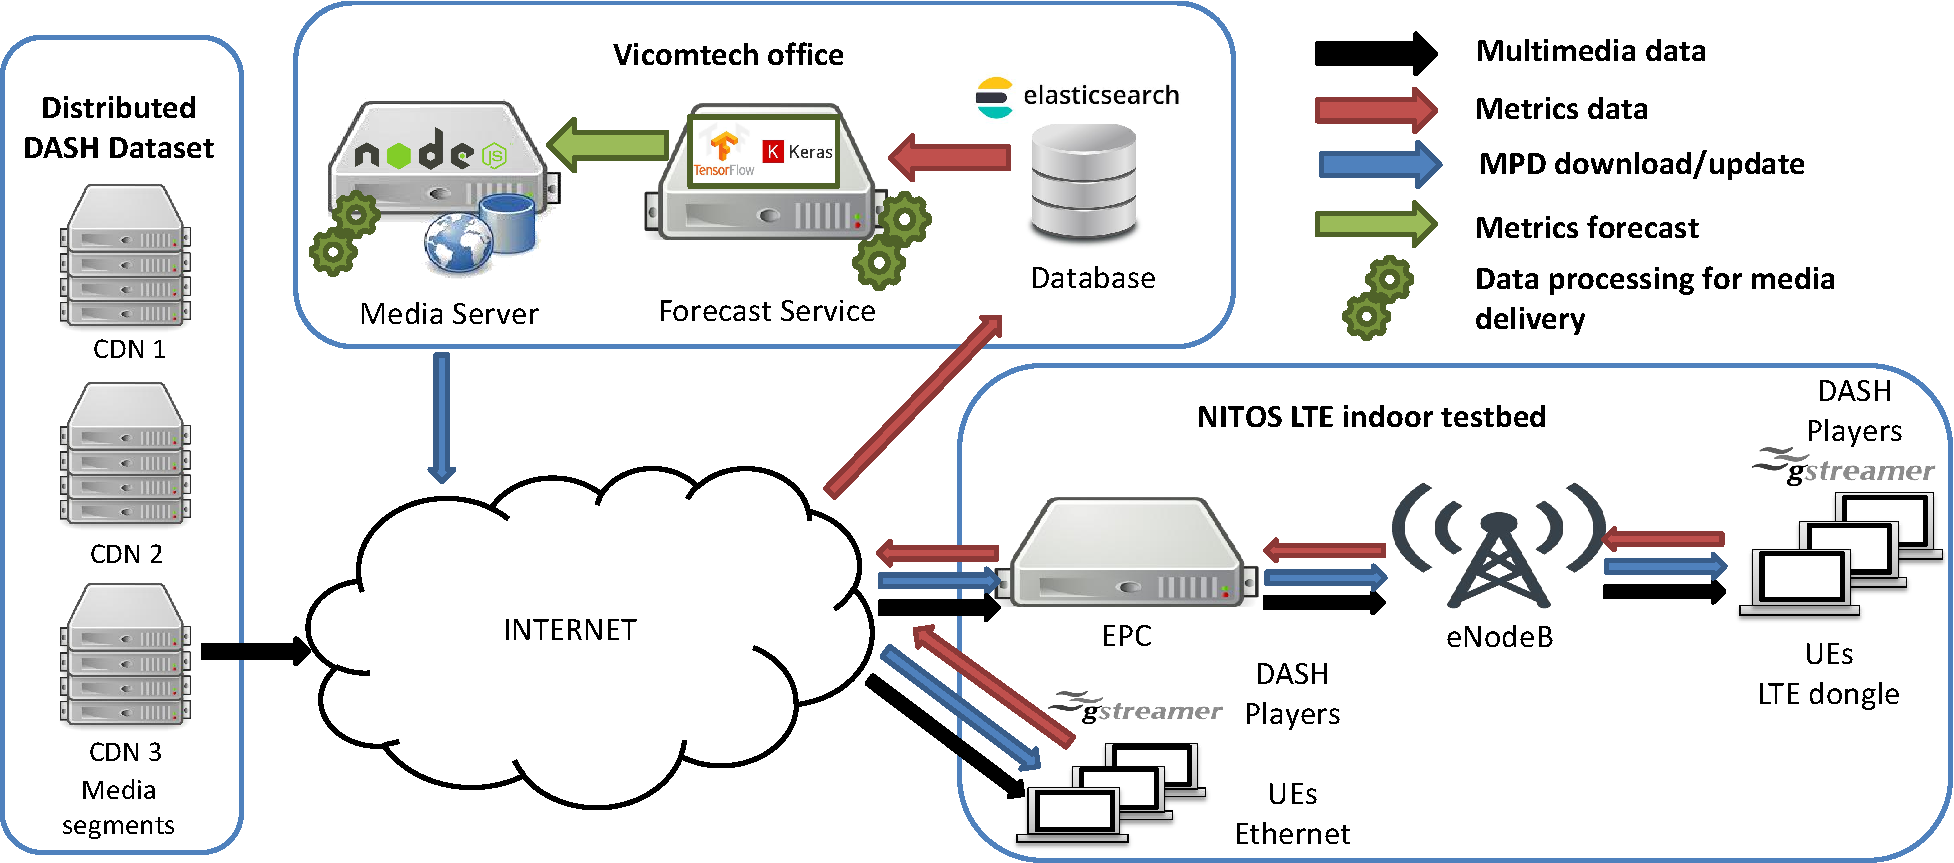
\includegraphics[width=1\textwidth,clip,keepaspectratio]{forecasting.pdf}%
		\label{fig:IEEETBC2020forecast}}
	\caption{Testbed setup: configurations for dataset creation (\textbf{a}) and for INFLOW enabled delivery (\textbf{b}).}
	\label{fig:IEEETBC2020setup}
\end{figure}

After the training phase is completed, a new setup for testing the proposed INFLOW solution is applied (\ref{fig:IEEETBC2020forecast}). Now, the collected metrics sent with a SAND-alike mechanism are consumed by the forecast service to execute bandwidth and latency predictions for the next period. The predictions are employed by the media server to apply its decision rules for CDN selection. In this case, the media server serves an MPD dynamically updated to force video players to periodically request it. The update period is equal to the segment duration (2 seconds) and it is set through the \textit{minimumUpdatePeriod} tag inside the MPD.

In this setup, we aimed to compare INFLOW with other CDN selection strategies. Then, we compared the results for the following common CDN selection strategies:
\begin{itemize}
	\item \textit{Single CDN (SC)}: this experiment does not involve multiple CDNs. It uses just the most affordable CDN for all the clients.
	\item \textit{Equal selection (ES)}: this experiment consists of balancing the occupancy rate of each CDN assigned when the session starts. Therefore, every CDN has the same number of connected clients, and the video players do not migrate between CDNs.
	\item \textit{Progressive selection (PS)}: this experiment consists of progressive allocation of new CDNs when the used one(s) gets exhausted, i.e., when the theoretical maximum number of connected clients is reached and the bandwidth from the SLA is consumed. The maximum number of clients is set to 33 (100 players / 3 CDNs). The clients do not migrate between CDNs.
	\item \textit{INFLOW selection (INFLOW)}: this experiment exploits the capabilities of the proposed INFLOW solution to dynamically migrate the clients depending on the predictions and the applicable cost ranges. It aims to minimize the use of CDN providers at any moment.
\end{itemize}

It is important to note that INFLOW needs to be set with the SLA for the clients to avoid any violation on QoS. Setting a bandwidth threshold lower than the minimum representation bitrate (100 kbps) is useless as the players should always experience at least the minimum representation bitrate to play the content. In the same way, a value higher than the maximum representation bitrate is not valid. Then, we decided to set the minimum bandwidth to 4 Mbps; this was enough to play a smooth 1080p video, which corresponds to two-thirds of the maximum available representation bitrate (6 Mbps).

\subsection{Validation and Results}
\label{sec:validation}

\subsubsection{Predictor validation}
\label{sec:mlmodel}

The generation of the LSTM model consisted of three steps: training, validation, and testing. Both the training and validation steps employed a training dataset, where 80\% of the samples were used for training and the remaining 20\% were used for the validation step. The training dataset consisted of a multivariate time series, and bandwidth and latency measurements were taken for three hours. The collection was performed in three different sessions lasting one hour each. Each session was executed on a different day and employed a different CDN to download the content. The testing process employed a testing dataset. The testing dataset consisted of the training dataset with an extra hour of data collected on a different day that was independent of the training dataset.

To guarantee that the LSTM model used equal spaced input measurements, the simple moving average (SMA) was applied to both datasets so that an average bandwidth and latency value could be computed each second. This resulted in 10800 samples for the training dataset and 3600 samples for the testing dataset. A total of 8640 samples of the training dataset (80\%) constituted the training set, while the remaining 2160 samples (20\%) were used as the validation set.

The training set was employed in the first phase to generate the LSTM model. The autocorrelation plot, depicted in Figure \ref{fig:IEEETBC2020autocorrelation}, shows a clear correlation of the tuple (bandwidth, latency) in the time series. Here, the autocorrelation is lower for samples that are more distant. Consequently, samples which are closer to the one we want to predict are the most valuable. The LSTM model provides next values based on the last \textit{N} bandwidth and latency measurements. \textit{N} has been empirically set to 7. A shorter window had a big impact on LSTM accuracy, while a longer one did not result in a significant increase in LSTM forecast fidelity. The accuracy results when \textit{N} = 6 dropped by 0.2\% for the bandwidth and by 2.7\% for the latency. The accuracy increased when \textit{N} = 8 was under 1\% for both time series.

\begin{figure}[htp]
	\centering
	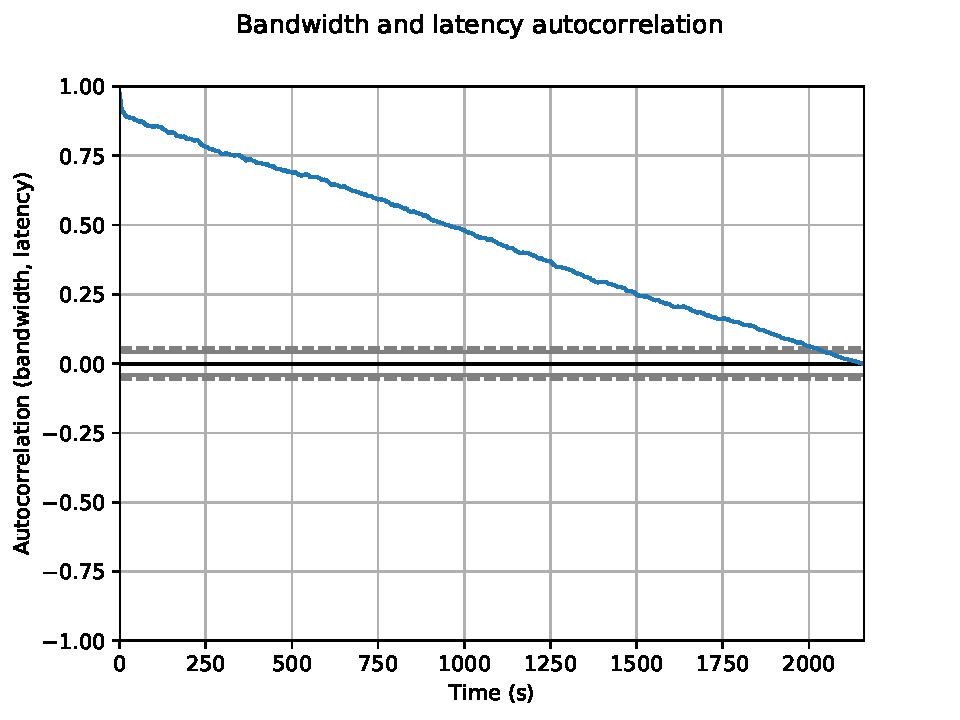
\includegraphics[width=1\textwidth,clip,keepaspectratio]{autocorrelation.pdf}
	\caption{Bandwidth and latency autocorrelation.}
	\label{fig:IEEETBC2020autocorrelation}
\end{figure}

A comparison of the values measured and predicted during the validation is shown in Figure \ref{fig:IEEETBC2020validation}. The graphs show that the predictor can follow the trend of the time series, but it cannot predict sudden and drastic changes (high or low outliers). We calculated the mean absolute error (MAE) and the root mean square error (RMSE) for both bandwidth and latency. The MAE values were 0.76 Mbps and 11 ms for bandwidth and latency, respectively, while the RMSE values were 0.99 Mbps and 27 ms, respectively.

\begin{figure}[htp]
	\centering
	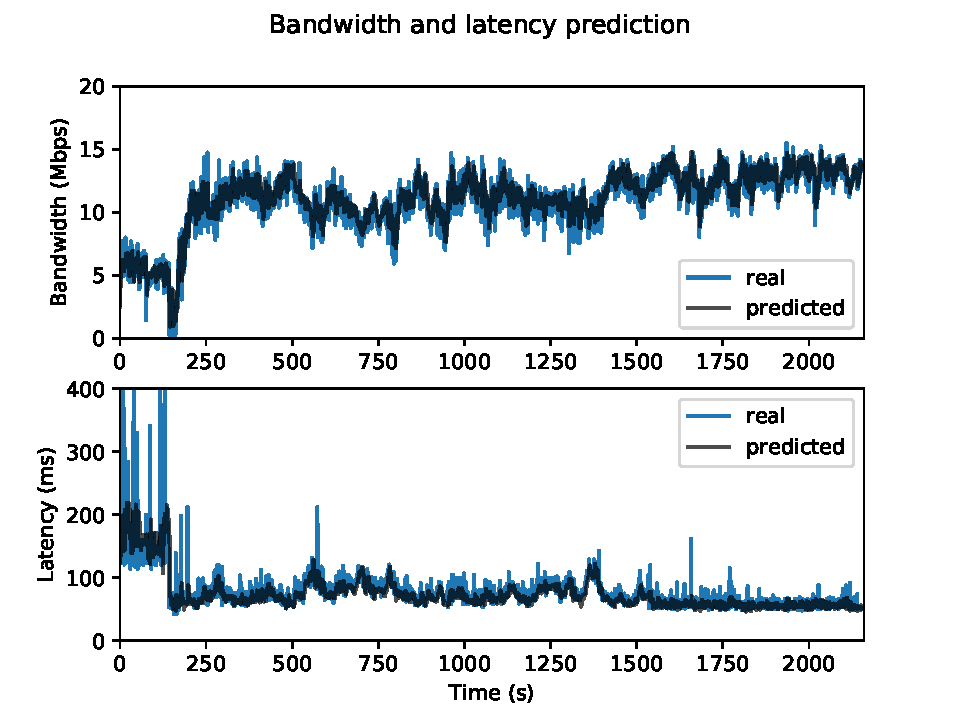
\includegraphics[width=1\textwidth,clip,keepaspectratio]{prediction_result2.pdf}
	\caption{Bandwidth and latency prediction: validation of the LSTM model.}
	\label{fig:IEEETBC2020validation}
\end{figure}

Once the model was validated, we generated the final model by training it with all the training dataset (10800 samples). Then, the final model was employed to predict values of the testing dataset. We limited the test to 2160 samples to foster a fair comparison with the validation results with a similar number of samples. For this subset, we compared the obtained values of MAE and RMSE with the ones coming from the previous validation. Figure \ref{fig:IEEETBC2020testing} shows the results of the testing process. The bandwidth MAE and RMSE were equal to 0.94 Mbps and 0.51 Mbps, respectively, which are definitely close (and even better) to the values obtained during the validation. On the contrary, the latency MAE and RMSE were 31 ms and 97 ms, respectively, making evident that the latency is harder to accurately predict. From the Figure \ref{fig:IEEETBC2020testing}, it is clear that latency produces higher outliers than the bandwidth, which are difficult to predict.

\begin{figure}[htp]
	\centering
	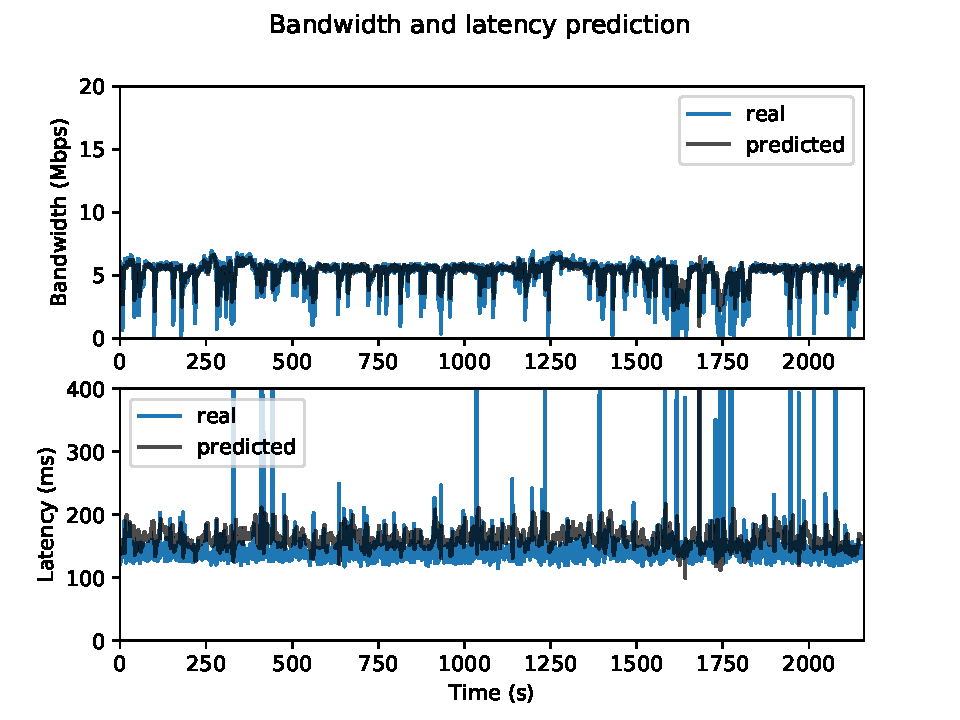
\includegraphics[width=1\textwidth,clip,keepaspectratio]{prediction_result.pdf}
	\caption{Bandwidth and latency prediction: testing of the trained LSTM model.}
	\label{fig:IEEETBC2020testing}
\end{figure}

\subsubsection{QoS performance comparison}
\label{sec:comparison}

INFLOW aims to manage the QoS performance and business cost trade-off. To this end, we identified different performance metrics for both the parameters to evaluate and balance them. We carried out the QoS evaluation by collecting the representation bitrate selected by the adaptation algorithm of the video players. Moreover, we compared the representation bitrate with the measured network bandwidth and latency to evaluate the efficiency of the utilization of the CDN resources as the efficiency increases as the overall throughput of a CDN approaches the available CDN bandwidth.

We tested our solution by comparing it with other CDN selection strategies. The final set of experiments utilized the \textit{single CDN (SC)}, \textit{equal selection (ES)}, \textit{progressive selection (PS)}, and \textit{INFLOW selection (INFLOW)} strategies. As mentioned in the previous section, the minimum bandwidth for \textit{INFLOW selection} algorithm was set to 4 Mbps, and the max amount of running players for each experiment was 100.

\begin{table}[t]
	\caption{Average value and standard deviation of the measured latency by the players.}
	\centering
	\bgroup
	\def\arraystretch{1.2}%  1 is the default, change whatever you need
	\setlength\tabcolsep{2.5pt} % default value: 6pt
	\label{tab:IEEETBC2020latency}
	\def\arraystretch{1.2}%  1 is the default, change whatever you need
	\setlength\tabcolsep{2.0pt} % default value: 6pt
	{\scriptsize
		\begin{tabular}{>{\centering\arraybackslash}m{\dimexpr0.18\textwidth-2\tabcolsep-\arrayrulewidth\relax}
				>{\centering\arraybackslash}m{\dimexpr0.13\textwidth-2\tabcolsep-\arrayrulewidth\relax}
				>{\centering\arraybackslash}m{\dimexpr0.13\textwidth-2\tabcolsep-\arrayrulewidth\relax}
				>{\centering\arraybackslash}m{\dimexpr0.13\textwidth-2\tabcolsep-\arrayrulewidth\relax}
				>{\centering\arraybackslash}m{\dimexpr0.13\textwidth-2\tabcolsep-\arrayrulewidth\relax}
				>{\centering\arraybackslash}m{\dimexpr0.13\textwidth-2\tabcolsep-\arrayrulewidth\relax}
				>{\centering\arraybackslash}m{\dimexpr0.13\textwidth-2\tabcolsep-\arrayrulewidth\relax}
		}
		\toprule
		\multirow{2}{*}{\textbf{Strategy}} & \multicolumn{2}{c}{\textbf{CDN1}} & \multicolumn{2}{c}{\textbf{CDN2}} & \multicolumn{2}{c}{\textbf{CDN3}} \\
		\cline{2-7}
		& \textbf{l$_{avg}$(ms)} & \textbf{l$_{dev}$(ms)} & \textbf{l$_{avg}$(ms)} & \textbf{l$_{dev}$(ms)} & \textbf{l$_{avg}$(ms)} & \textbf{l$_{dev}$(ms)} \\
		\midrule
		\midrule
		Single CDN & 89 & 39 & - & - & - & - \\
		Equal selection & 89 & 42 & 132 & 35 & 42 & 25 \\
		Progressive selection & 85 & 35 & 127 & 23 & 51 & 157 \\
		INFLOW selection & 114 & 68 & 125 & 54 & 94 & 75 \\
		\bottomrule
		\bottomrule
	\end{tabular}
	\egroup
	}
\end{table}

\begin{table}[t]
	\caption{Average value and standard deviation of the measured bandwidth by the players.}
	\centering
	\bgroup
	\def\arraystretch{1.2}%  1 is the default, change whatever you need
	\setlength\tabcolsep{2.5pt} % default value: 6pt
	\label{tab:IEEETBC2020bw}
	\def\arraystretch{1.2}%  1 is the default, change whatever you need
	\setlength\tabcolsep{2.0pt} % default value: 6pt
	{\scriptsize
		\begin{tabular}{>{\centering\arraybackslash}m{\dimexpr0.18\textwidth-2\tabcolsep-\arrayrulewidth\relax}
			>{\centering\arraybackslash}m{\dimexpr0.13\textwidth-2\tabcolsep-\arrayrulewidth\relax}
			>{\centering\arraybackslash}m{\dimexpr0.13\textwidth-2\tabcolsep-\arrayrulewidth\relax}
			>{\centering\arraybackslash}m{\dimexpr0.13\textwidth-2\tabcolsep-\arrayrulewidth\relax}
			>{\centering\arraybackslash}m{\dimexpr0.13\textwidth-2\tabcolsep-\arrayrulewidth\relax}
			>{\centering\arraybackslash}m{\dimexpr0.13\textwidth-2\tabcolsep-\arrayrulewidth\relax}
			>{\centering\arraybackslash}m{\dimexpr0.13\textwidth-2\tabcolsep-\arrayrulewidth\relax}
		}
		\toprule
		\multirow{2}{*}{\textbf{Strategy}} & \multicolumn{2}{c}{\textbf{CDN1}} & \multicolumn{2}{c}{\textbf{CDN2}} & \multicolumn{2}{c}{\textbf{CDN3}} \\
		\cline{2-7}
		& \textbf{bw$_{avg}$(Mbps)} & \textbf{bw$_{dev}$(Mbps)} & \textbf{bw$_{avg}$(Mbps)} & \textbf{bw$_{dev}$(Mbps)} & \textbf{bw$_{avg}$(Mbps)} & \textbf{bw$_{dev}$(Mbps)} \\
		\midrule
		\midrule
		Single CDN & 2.54 & 0.44 & - & - & - & - \\
		Equal selection & 2.66 & 0.41 & 15.50 & 7.16 & 11.42 & 2.76 \\
		Progressive selection & 2.90 & 0.34 & 21.84 & 4.79 & 10.65 & 2.17 \\
		INFLOW selection & 3.52 & 2.43 & 5.23 & 3.85 & 5.88 & 2.82 \\
		\bottomrule
		\bottomrule
	\end{tabular}
	\egroup
	}
\end{table}

\begin{table*}[t]
	\caption{Average value and standard deviation of the selected bitrate by the players.}
	\centering
	\bgroup
	\def\arraystretch{1.2}%  1 is the default, change whatever you need
	\setlength\tabcolsep{2.5pt} % default value: 6pt
	\label{tab:IEEETBC2020quality}
	\def\arraystretch{1.2}%  1 is the default, change whatever you need
	\setlength\tabcolsep{2.0pt} % default value: 6pt
	{\scriptsize
		\begin{tabular}{>{\centering\arraybackslash}m{\dimexpr0.18\textwidth-2\tabcolsep-\arrayrulewidth\relax}
				>{\centering\arraybackslash}m{\dimexpr0.13\textwidth-2\tabcolsep-\arrayrulewidth\relax}
				>{\centering\arraybackslash}m{\dimexpr0.13\textwidth-2\tabcolsep-\arrayrulewidth\relax}
				>{\centering\arraybackslash}m{\dimexpr0.13\textwidth-2\tabcolsep-\arrayrulewidth\relax}
				>{\centering\arraybackslash}m{\dimexpr0.13\textwidth-2\tabcolsep-\arrayrulewidth\relax}
				>{\centering\arraybackslash}m{\dimexpr0.13\textwidth-2\tabcolsep-\arrayrulewidth\relax}
				>{\centering\arraybackslash}m{\dimexpr0.13\textwidth-2\tabcolsep-\arrayrulewidth\relax}
		}
		\toprule
		\multirow{2}{*}{\textbf{Strategy}} & \multicolumn{2}{c}{\textbf{CDN1}} & \multicolumn{2}{c}{\textbf{CDN2}} & \multicolumn{2}{c}{\textbf{CDN3}} \\
		\cline{2-7}
		& \textbf{R$_{avg}$(Mbps)} & \textbf{R$_{dev}$(Mbps)} & \textbf{R$_{avg}$(Mbps)} & \textbf{R$_{dev}$(Mbps)} & \textbf{R$_{avg}$(Mbps)} & \textbf{R$_{dev}$(Mbps)} \\
		\midrule
		\midrule
		Single CDN & 1.67 & 0.62 & - & - & - & - \\
		Equal selection & 1.78 & 0.67 & 4.46 & 2.10 & 4.77 & 1.71 \\
		Progressive selection & 1.96 & 0.61 & 5.10 & 1.78 & 4.48 & 1.98 \\
		INFLOW selection & 1.96 & 1.23 & 2.44 & 1.57 & 2.82 & 1.43 \\
		\bottomrule
		\bottomrule
	\end{tabular}
	\egroup
	}
\end{table*}

Table \ref{tab:IEEETBC2020latency} shows the network latency for the video players. The results for each CDN while employing \textit{SC}, \textit{ES}, and \textit{PS} strategies are close to each other. Each CDN presents similar latency independently of the strategy. On the contrary, \textit{INFLOW} strategy presents a higher latency of up to +124\% (CDN3) as switching the connection from a CDN to another inevitably implies the addition of delay. Furthermore, if the experienced latency is still in the order of hundreds of milliseconds, then it does not affect the video players, which have a playback buffer equal to one segment duration (2 seconds).

Table \ref{tab:IEEETBC2020bw} shows the available network bandwidth for the video players while video content is being downloaded from the CDNs. Table \ref{tab:IEEETBC2020quality} presents the selected bitrate from the client-side algorithm.

\textit{SC} strategy provides only information for CDN1 as the other two are never used. This strategy provides the worst results when compared to the others because the players are experiencing a highly congested CDN communication. The average measured bandwidth is 2.54 Mbps, and average representation bitrate is 1.67 Mbps.

As expected, \textit{SC} results improve when the multi-CDN strategy comes into place, therefore allowing for load balancing. \textit{ES} and \textit{PS} strategies limit to 33 (100 players / 3 CDNs) the number of players connected to CDN1. Both strategies produce similar results for the different CDNs. For CDN1, the average measured bandwidth of \textit{ES} and \textit{PS}, when compared to \textit{single CDN} strategy, improves +4.7\% and +14.1\%, respectively. These results mean a higher bitrate selection, +6.6\% and +17.4\%, respectively. Moreover, the selected bitrates are considerably higher for CDN2 and CDN3 as they provide a higher performance. These CDNs provide more network resources serving higher bandwidths for video players. The measured results range between 15.50 Mbps (\textit{ES}) and 21.84 (\textit{PS}) for CDN2 and 10.65Mbps (\textit{PS}) and 11.42 (\textit{ES}) for CDN3. Thus, distributing video players across the available CDNs by just considering the number of players per CDN (33 players) is not fair as video players connected to CDN2 and CDN3 can select higher representation bitrates. Video players select a representation bitrate up to +160\% higher if connected to CDN2 and +168\% higher if connected to CDN3.

\textit{INLFOW} uses a different approach. Here, the maximum number of players for each CDN is constantly updated through Equation \ref{eq:IEEETBC2020players}. Then, video players are dynamically switched at any time. CDN1 still underperforms compared to CDN2 and CDN3, but the fairness is lower. The residual performance bias is due to the fact that CDN1 is still the preferred CDN, i.e., the other two are not used until CDN1 is congested. Accordingly, CDN3 is not used until CDN2 is congested too. Here, the higher average measured bandwidth is 5.88 Mbps at CDN3, which is +67\% higher than the result at CDN1 (3.52 Mbps). For \textit{ES} and \textit{PS}, the variations are +483\% (CDN2 compared to CDN1) and 653\% (CDN2 compared to CDN1), respectively. In terms of the selected representation bitrate, \textit{INFLOW} keeps the results obtained by the other multi-CDN strategies at CDN1 but underperforms at CDN2 and CDN3. This is because INFLOW aims to reduce the number of employed CDNs and the OPEX at any time, while guaranteeing at least 4 Mbps for the measured network bandwidth. Thus, video sessions to CDN2 or CDN3 can be retired, therefore saving the CDN OPEX. The other multi-CDN strategies do not reduce CDN usage, i.e., when the player is connected to a CDN, the connection is maintained until the session expires. In terms of fairness, \textit{INFLOW} outperforms the other multi-CDN strategies as the average representation bitrates of each CDN are close to each other. Video players connected to CDN2 present the best representation bitrate (2.44 Mbps), which is +24\% higher than those of video players connected to CDN1. Moreover, standard deviation for measured bandwidth and representation bitrate achieved with INFLOW also demonstrates that it is the fairest solution since the players experience almost the same variation independently of the CDN. Standard deviation for CDN2 is +58\% higher than CDN1 if we consider measured bandwidth and +27\% if we consider representation bitrate.

Concerning communications overheads to proactively enforce QoS, the traffic overhead is 893 MB from the total traffic (53592 MB). Thus, overhead causes an increase of +1.6\% in the transmitted data. INFLOW exploits MPD update mechanism with an update period is equal to the segment duration. In our case this means 9040 Bytes requested every 2 seconds by each player. In the other strategies, MPD update mechanism is not used, then there is not an additional overhead.

The predictions performed by the INFLOW Forecast service during the MPD requests causes also higher MPD delivery delay compared to the other strategies. As a result, INFLOW strategy adds 53 ms of delay while delivering the MPD. Nevertheless, this delay does not affect the playback since the player employs the previous MPD until a new one is received and parsed. Thus, if it is necessary to perform a segment request during an MPD update, it is performed in any case, as the two operations are executed in different threads and do not interfere with each other. In terms of resource utilization, the node running the INFLOW Forecast service shown 3.2 GB RAM, 33\% CPU and 27\% GPU peak utilization rates. Thus, its hardware configuration could absorb a larger number of users.

\subsubsection{Business cost comparison}
\label{sec:metrics}

Regarding business cost, OPEX consists of ongoing expenses that a business incurs inherent to the operation of the assets. In our case, we were interested in OPEX, as we wanted to evaluate the cost of the CDN resources due to their ongoing utilization, i.e., it depends on the utilization of the CDN resources at any time \cite{verbrugge2006}.

There is no common formula for evaluating the OPEX, as in many cases, the provider does not publish publicly its pricing plans, but it offers personalized plans to each customer. Nevertheless, \cite{dacast2019}, \cite{CdnCalculator} and \cite{wowza} reveal that the OPEX for CDN resources depends on a set of factors such as the employed network, storage, and time resources. Then, we express monthly OPEX through Equation \ref{eq:IEEETBC2020opex}.

\begin{equation}
\label{eq:IEEETBC2020opex}
\begin{split}
OPEX_{month} = \sum_{i=1}^{K} & \alpha_{loc_i}*Tr_i + \beta_{loc_i}*K_{req_i} + \\
& + \gamma_{loc_i}*T_i + \delta_{loc_i}*St_i + \epsilon_{loc_i}
\end{split}
\end{equation}

In the equation, \textit{Tr$_i$} is the traffic volume in a month, \textit{K$_{req_i}$} is the number of HTTP requests producing such demand, \textit{T$_i$} is the utilization time for a CDN that has active sessions from video players of a service, and \textit{St$_i$} is the employed storage at the CDN. Therefore, $\alpha_{loc_i}$, $\beta_{loc_i}$, $\gamma_{loc_i}$, $\delta_{loc_i}$, and $\epsilon_{loc_i}$ are multiplicative coefficients established by a particular CDN provider and that depend on the location of the resources (cost of the servers depends on the country where they are located). The addition indicates that we are in multi-CDN environment. Then, we need to sum over the \textit{K} available CDNs.

The values for the coefficients are closely related to the business model and the pricing plan of each CDN provider. Accordingly, the monthly OPEX is tailored to the employed CDNs. In any case, we evaluate the variables independent of the CDN vendor, which depend on the resources we are employing during the tests (\textit{Tr$_i$}, \textit{K$_{req_i}$}, \textit{T$_i$} and \textit{St$_i$}) and directly impact the OPEX.

To simplify the evaluation of OPEX, we have made some assumptions. First, \textit{St$_i$} is fixed for each experiment as the amount of employed storage depends on the content size, and it is permanently stored, even if it is never requested. Second, \textit{K$_{req_i}$} is almost constant as, in any case, the experiments run 100 players, which request a media segment and an MPD every 2 seconds (segment duration). Third, \textit{Tr$_i$} is directly proportional to the selected representation bitrate. It can be roughly calculated by multiplying the mean bitrate of the sessions from video players and the duration of the experiment. As the selected bitrate is already being captured for the QoS evaluation, we can assess the traffic volume. Finally, \textit{T$_i$} is the variable that really changes across every experiment depending on the cost-effective strategy, leading to different utilization rates for each available CDN. Then, we employ \textit{T$_i$} as the main metric for comparing the OPEX achieved by the different strategies.

\begin{table}[htp]
	\caption{Utilization time of the CDNs.}
	\centering
	\bgroup
	\def\arraystretch{1.2}%  1 is the default, change whatever you need
	\setlength\tabcolsep{2.5pt} % default value: 6pt
	\label{tab:IEEETBC2020time}
	\def\arraystretch{1.2}%  1 is the default, change whatever you need
	\setlength\tabcolsep{2.0pt} % default value: 6pt
	{\scriptsize
		\begin{tabular}{>{\centering\arraybackslash}m{\dimexpr0.18\textwidth-2\tabcolsep-\arrayrulewidth\relax}
			>{\centering\arraybackslash}m{\dimexpr0.13\textwidth-2\tabcolsep-\arrayrulewidth\relax}
			>{\centering\arraybackslash}m{\dimexpr0.13\textwidth-2\tabcolsep-\arrayrulewidth\relax}
			>{\centering\arraybackslash}m{\dimexpr0.13\textwidth-2\tabcolsep-\arrayrulewidth\relax}
		}
		\toprule
		\multirow{2}{*}{\textbf{Strategy}} & \textbf{CDN1} & \textbf{CDN2} & \textbf{CDN3} \\
		\cline{2-4}
		& \textbf{T$_{i}$(minutes)} & \textbf{T$_{i}$(minutes)} & \textbf{T$_{i}$(minutes)} \\
		\midrule
		\midrule
		Single CDN & 60 & - & - \\
		Equal selection & 59 & 59 & 58 \\
		Progressive selection & 58 & 58 & 57 \\
		INFLOW selection & 52 & 48 & 31 \\
		\bottomrule
		\bottomrule
	\end{tabular}
	\egroup
	}
\end{table}

Table \ref{tab:IEEETBC2020time} shows the usage time of each CDN while applying the different strategies. \textit{ES} strategy is the most expensive solution as all the CDN are utilized almost all the time. In this case, the overall usage time is close to 3 h (1 h per each CDN). The actual result is 176 min. On the contrary, \textit{SC} results in lower business costs as CDN2 and CDN3 are never employed. In this case, the usage time is just 60 min. \textit{PS} is quite like \textit{ES}. Figure \ref{fig:IEEETBC2020experiments2} shows the number of players connected to each CDN for one hour and it is clear that \textit{ES} and \textit{PS} differ only in the first minutes. In \textit{ES}, the three curves increase almost together, while in \textit{PS}, the curves separately increase because CDN2 is not employed until CDN1 reaches 33 players and CDN3 is only employed after both CDN1 and CDN2 reach 33 players. The overall usage time is 173 min, which corresponds to a reduction of -2\% compared to \textit{ES}. From Table \ref{tab:IEEETBC2020time}, the usage time of each CDN while employing PS strategy is similar to ES one. Finally, \textit{INFLOW} graph presents a completely different behavior. Here, the number of players connected at each CDN is much more variable owing to the switching mechanism. The number of players of each CDN ranges between 0 (the CDN is not being used) to 100 (CDN serving all the players). The number of players for the other multi-CDN strategies is always around 33 players. Nevertheless, INFLOW can retire the sessions from a CDN, which is not necessary after migrating the clients. This results in 131 min of overall usage time; then the reductions for \textit{ES} and \textit{PS} are -26\% and -24\%, respectively. Compared to \textit{SC} strategy, \textit{INFLOW} employs +118\% more CDN usage time, while the value increases to +193\% and +183\% for \textit{ES} and \textit{PS}, respectively If we focus on the usage time of each CDN, Table \ref{tab:IEEETBC2020time} clearly shows that INFLOW reduces the usage of CDN2 and CDN3.

\begin{figure}[htp]
	\centering
	\subfloat[]{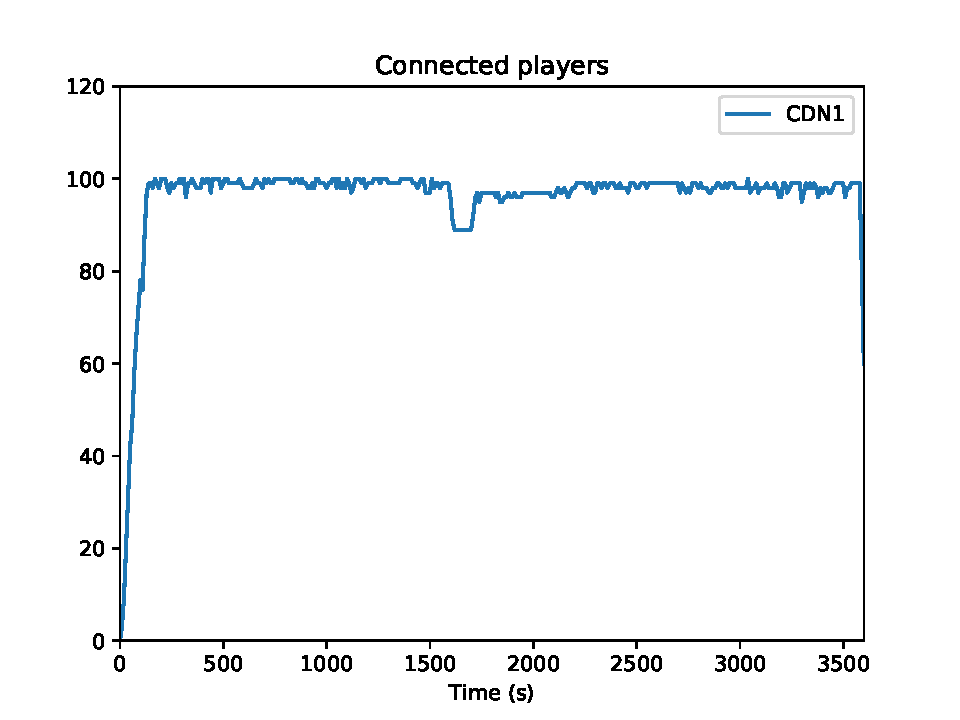
\includegraphics[width=3in,clip,keepaspectratio]{single_server_players.pdf}%
		\label{fig:IEEETBC2020experiments2a}}
%	\hfil
	\subfloat[]{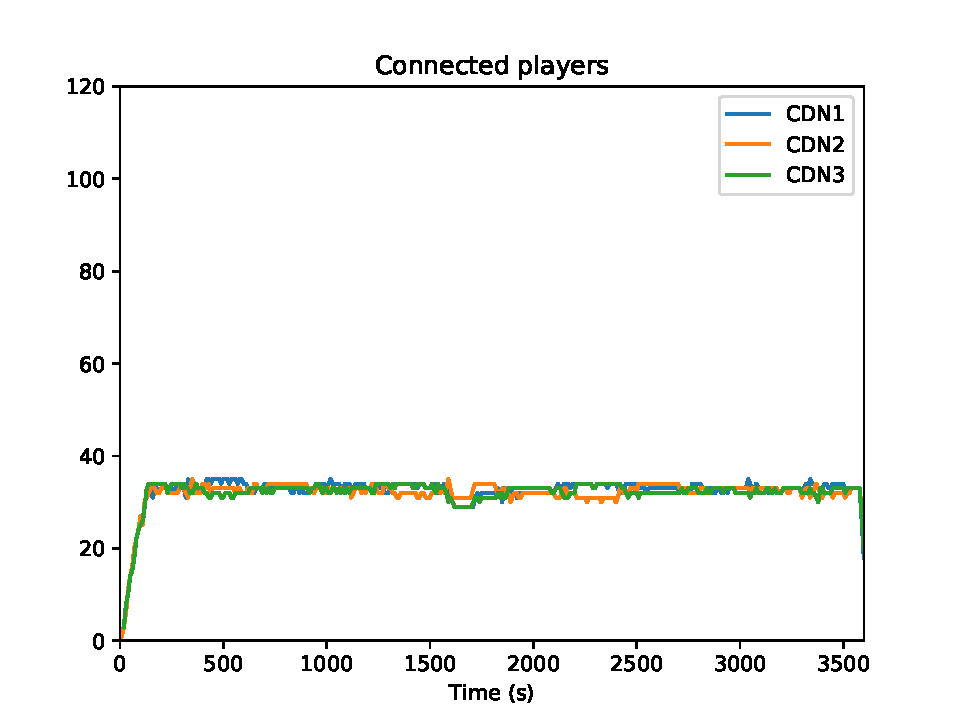
\includegraphics[width=3in,clip,keepaspectratio]{three_equal_players.pdf}%
		\label{fig:IEEETBC2020experiments2b}}
	\hfil
	\subfloat[]{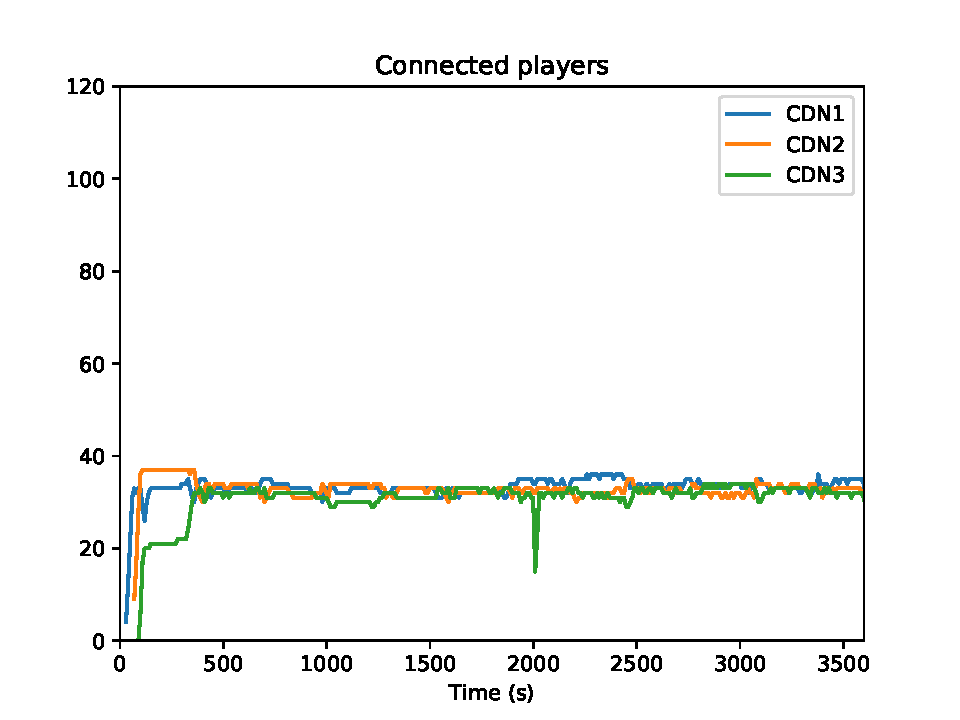
\includegraphics[width=3in,clip,keepaspectratio]{three_progressive_players.pdf}%
		\label{fig:IEEETBC2020experiments2c}}
%	\hfil
	\subfloat[]{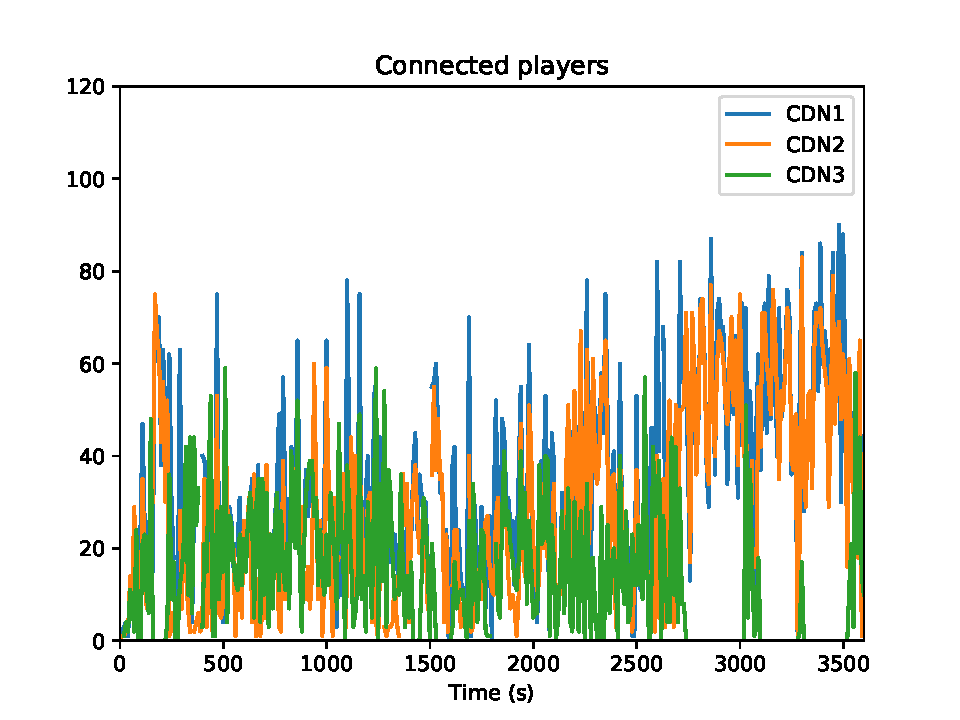
\includegraphics[width=3in,clip,keepaspectratio]{dynamic_4Mbps_players.pdf}%
		\label{fig:IEEETBC2020experiments2d}}
	\caption{Distribution of the players among the available CDNs: single CDN (\textbf{a}), equal selection (\textbf{b}), progressive selection (\textbf{c}) and INFLOW selection (\textbf{d}) strategies.}
	\label{fig:IEEETBC2020experiments2}
\end{figure}

In summary, the proposed INFLOW solution improves the CDN resource management by dynamically selecting the CDN for each video player at any time. It allows for business cost saving by decreasing the usage time of the available CDNs, while maintaining a minimum bandwidth level. Moreover, the resources are more efficiently exploited because the players are distributed depending on the real capabilities of each CDN, such as the experienced network resources. Consequently, the selected bitrate is fairer among the players.


\subsection{Conclusions and Future Work}
\label{sec:conclusion}
The trend for the following years is an increasing consumption of media content, where the content is mostly delivered through CDN infrastructure. Here, the CP strives to guarantee the necessary QoS for its media service while reducing the business costs associated with the CDN.

Toward this goal, we introduce a novel solution called INFLOW for CDN selection in a multi-CDN delivery environment. INFLOW enables the media server with a forecast service so that metrics collected by the player are processed as MPEG-DASH streams are served. The forecast service executes time series analysis through an LSTM model for prediction of the future values of network bandwidth and latency. The predictions are exploited by the media server to act while the player requests an MPD update. The media server can decide to keep the same MPD or change it to switch the player to another available CDN from which content can be downloaded.

The proposed solution has been implemented and validated in a distributed and heterogeneous testbed employing real network nodes. The evaluation includes a comparison with other CDN selection strategies in terms of QoS and business cost. The results highlight the advantages of INFLOW for reducing the overall usage time of the available CDNs, while guaranteeing a minimum level of network bandwidth to every player.

Future work includes the exploitation of new metrics to improve the predictions made by the forecast service. Moreover, the collected metrics can be further exploited to obtain an estimation of a user's QoE, and actions that also take into consideration the user's expectations can be taken.


% use section* for acknowledgment
\subsection*{Acknowledgment}
\label{sec:ackIEEEA}
This work was fully supported by the EC projects Fed4Fire+, 732638 (H2020-ICT-13-2016, Research and Innovation action) and Open-VERSO project (Red Cervera program, Spanish government's Centre for the Development of Industrial Technology).


%Introduction
%\begin{savequote}[50mm]
%If our brains were simple enough for us to understand them, we'd be so simple that we couldn't.
%\qauthor{Ian Stewart }%The Collapse of Chaos: Discovering Simplicity in a Complex World
%\end{savequote}
%[Two-way complementarity of computing capabilities]
%\chapter{Two-way complementarity of computing capabilities in multi-device media services}
\chapter{MEC-enabled content delivery}
\chaptermark{MEC-enabled content delivery}
\label{chap:MEC}

\section{Context}

MEC is a new network architecture concept included in the 5G ecosystem to boost the performance of network services. It enables computing capability close to the RAN such to run algorithms and/or services that empower specific applications. Moreover, RNI Service (RNIS) integrated into MEC platform allows to access RAN information or RNI, a set of objective metrics (QoS) concerning the status of the UE connected through radio interface. When considering video streaming, having only QoS metrics is not enough. It is useful to assess or estimate the QoE experienced by the users and take actions to improve their individual QoE and the fairness among them in the exploitation of network resources. Maximizing customer satisfaction through QoE-based networking is a crucial challenge for video streaming services. ETSI working documents also support the application of analytics at the MEC to optimize the video streaming traffic.

Section \ref{chap:MTAP2020} proposes a MEC-enabled MPEG-DASH video streaming proxy that estimates the users' QoE according to ITU-T P.1203. It is derived from monitored QoS metrics in a dense client radio cell and the information acquired by accessing the MPEG-DASH manifest (MPD). It does not need an explicit out of band messaging from video players to MEC system. Thus, the implemented MEC proxy is independent of video servers and players. Knowledge of QoE can enable advanced solutions that realize the network/application symbiosis, as it provides the information to subsequently decide streaming qualities in a coordinated manner in a dense client cell. The major contributions of this paper can be summarized as follows:
\begin{itemize}
	\item A novel mechanism to estimate ITU-T P.1203 QoE scores from network dynamics at the cell and parameters parsed from MPEG-DASH MPD without an explicit out of band messaging from video players to MEC system. It aims to assess information of video representation bitrates, number of representation switches, number of stalling events and their duration.
	\item An implementation of a MEC proxy, independent from video servers and players, to monitor and assess ITU-T P.1203 QoE scores for each local session.
	\item The analysis of the accuracy of the proposed solution to assess the ITU-T P.1203 QoE of individual players in a Wi-Fi-based experimentation setup and a dense client cell. To this end, two scenarios with different levels of concurrency and congestion are performed.
	%The first scenario has 10 players at a time, while in the second one the number of players is increased to 20.
\end{itemize}
Concerning stall assessment, the MEC proxy cannot detect all the stalls experienced by the player. In any case, the total duration of stalls tends to converge to the actual accumulated value experienced by the player. The MEC proxy cannot detect micro-stalls and tends to concentrate several of them into a macro-stall. This behavior is due to the sampling time to check for stalls (segment duration of 6 seconds). If two micro-stalls are experienced during the same segment, MEC proxy will conjecture that just one longer stall happened since it checks only at the end of each segment download.
The results in terms of QoE scores obtained at the MEC are compared with the actual ones achieved at the player side. Mean Absolute Error (MAE) and Root Mean Square Error (RMSE) rates show that the scores obtained at the MEC tend to be like the ones at the player. It demonstrates the capability of the MEC Proxy to estimate ITU-T P.1203 QoE scores close to actual ones.

In Section \ref{chap:BMSB2018}, information available at the MEC location is exploited to develop a MEC solution, called MEC4CDN, that allows two different operations. First, MEC4CDN caches popular MPEG-DASH segments at network edge to reduce CDN usage. To this end, it is able to identify recurrent requests. Second, it shields from identified or predicted CDN malfunction by switching the download of MPEG-DASH segments to an alternative CDN in order to ensure QoE rates. Thus, it enables a CDN dynamic selection based on live connectivity statistics. In both operations, the information of MPEG-DASH MPD is essential to know the available representations, as well as the location of the remote CDN servers. This paper comprises the following relevant contributions:
\begin{itemize}
	\item Local cache at the MEC of the identified contents to minimize the traffic between the CDN and the network edge. MEC4CDN decides to locally cache already served responses to serve near future requests and proactively cache the identified future segments in case of VOD streams.
	\item Dynamic selection of the CDN based on live measurements in the context of a multi-CDN delivery. The player starts receiving the stream from a CDN server, that is favorable in terms of QoS connectivity metrics, and is dynamically switched to another one which provides better performance in case of CDN degradation or outage.
	\item Evaluation by delivering MPEG-DASH streams in a dense client cell
	%having 20 players
	and comparing the two proposed strategies (local cache and dynamic CDN selection) with a legacy stream delivery.
\end{itemize}
Concerning local cache strategy, the results show that MEC4CDN lets the player experience lower latency since the segments are closer to it, then the throughput is higher. Therefore, the players tend to request higher representation bitrates which improve the user's QoE.
When considering dynamic CDN selection strategy, legacy MPEG-DASH delivery does not let the player take actions when the principal CDN suffers performance degradation. The player has to reduce the representation bitrate in order to continue playing. On the contrary, when MEC4CDN comes into play, it switches player's connection to a healthy CDN such that the representation bitrate is kept to higher levels. Therefore, MEC4CDN is able to enforce the delivery by switching to an alternative CDN which better performs.
To sum up, both strategies present advantages over a legacy MPEG-DASH delivery. When network issues are experienced, they allow to keep the QoE rates (CDN switching) or even improve them (local cache at the edge).
% !TeX spellcheck = en_US
%Publications.tex
%\newcommand{\PublicationsPath}{PatentsAndPublications/Publications}

%MTAP2020

\section[Multi-access Edge Computing video analytics of ITU-T P.1203 Quality of Experience for streaming monitoring in dense client cells]{Multi-access Edge Computing video analytics of ITU-T P.1203 Quality of Experience for streaming monitoring in dense client cells}
\label{chap:MTAP2020}
\begin{itemize} \itemsep1pt\parskip0pt\parsep0pt
	\item \textbf{Title:} Multi-access Edge Computing video analytics of ITU-T P.1203 Quality of Experience for streaming monitoring in dense client cells
	\item \textbf{Authors:} Roberto Viola, Mikel Zorrilla, Pablo Angueira and Jon Montalb\'an
	\item \textbf{Journal:} Multimedia Tools and Applications
	\item \textbf{Publisher:} Springer
	\item \textbf{Year:} (Submitted March 25, 2021)
%	\item \textbf{DOI:}  \url{}
\end{itemize}	

\textbf{Abstract:} 5G promises unseen network rates and capacity. Furthermore, 5G ambitions agile networking for specific service traffic catalysing the application and network symbiosis. Nowadays, the video streaming services consume lots of networking assets and produce high dynamics caused by players mobility meaning a challenging traffic for network management. The Quality of Experience (QoE) metric defined by \hbox{ITU-T P.1203} formulates the playback issues related to widely employed Dynamic Adaptive Streaming over HTTP (DASH) technologies based on a set of parameters measured at the video player. Monitoring the individual QoE is essential to dynamically provide the best experience to each user in a cell, while video players compete to enhance their individual QoE and cause high network performance dynamics. The edge systems have a perfect position to bring live coordination to dense and dynamic environments, but they are not aware of QoE experienced by each video player. This work proposes a mechanism to assess QoE scores from network dynamics at the cell and manifests of DASH streams without an explicit out of band messaging from video players to edge systems. Hence, this paper implements an edge proxy, independent from video servers and players, to monitor and estimate QoE providing the required information to later decide streaming qualities in a coordinated manner in a dense client cell. Its lightweight computation design provides real-time and distributed processing of local sessions. To check its validity, a WiFi setup has been exercised where the accuracy of the system at the edge is checked by assessing the ITU-T P.1203 QoE of individual players.

\textbf{Keywords:} 5G, MEC, MOS, MPEG-DASH, QoE.

\subsection{Introduction}
\label{intro}

Popularity of video streaming platforms to consume live sports events and over-the-top (OTT) services like Netflix, when combined with mobility and city contexts, result in a complex traffic congestion scenario to be managed. Specifically, when video players share the same path, they try to individually enhance their Quality of Experience (QoE) considering instant available bandwidth and display setup. As the cell gets more subscribers and the Base Station (BS) serves more traffic sessions, dynamics turn higher and available bandwidth estimation at client side gets coarser, fuelling video player fluctuations on requested bandwidth which affect the QoE \cite{khan2018}. Therefore, when congestion at the radio link comes into place, a dense client cell means a pool of clients competing for the available network assets. This competition leads to player instability, unfairness between players, and bandwidth under-utilization \cite{akhshabi2012}.

Maximizing customer satisfaction through QoE-based networking is a crucial challenge for video streaming services.
As most of the traffic flooding the networks comes from video streaming services, Mobile Network Operators (MNOs) need to configure the network according to cost-effective policies to cope with video demand while providing best QoE with the available resources.
To this end, MNOs need to monitor the QoE without access to video streaming servers, Content Delivery Network (CDN) systems or video player applications.

In the upcoming horizon 5G aims to improve current Key Performance Indicators (KPIs), such as traffic density, volume and latency. It will flatten barriers to allow network operators and/or 3rd parties to provide dynamic networking performance to respond to specific traffic demands \cite{etsits5g}.
To this end, network management frameworks analyse network assets and traffic features to adapt network setup to concurrent traffic needs. This means a revolution on networks with a digital transformation which leaves behind the concept one-fits-all and moves to a specialized and mutable network which dynamically changes its configuration over a common bare-metal infrastructure.

In the line of catalysing synergies of network and traffic from services, edge computing is gaining relevance due to benefits of local processing. Enabled by the transition of networking assets to cloud infrastructures, the provision of hosting at the edge means new revenues for MNOs. Furthermore, the location of some parts or entire systems of a service closed to the clients enables advanced possibilities considering the user environment. The application of analytics at the edge to optimise the video streaming traffic is a use case compiled in the ETSI working documents as a key representative of Multi-access Edge Computing (MEC) application \cite{etsigsmec002}.

The proposed 5G MEC-enabled proxy estimates the end users' QoE according to ITU-T P.1203 \cite{itup1203} and derived from monitored QoS metrics in the radio cell to allow a decision by other edge services operating streaming qualities in a coordinated manner in a dense client cell. Thus, the proposed system catalyses the use of Video Streaming Analytics at the network edge to realise the network/application symbiosis \cite{etsigsmec002}.

The major contributions of this paper can be summarized as follows:
\begin{itemize}
	\item A novel mechanism to estimate ITU-T P.1203 \cite{itup1203} QoE values from network dynamics at the cell and parameters parsed from manifests of DASH streams without an explicit out of band messaging from video players to edge system.
	\item A lightweight implementation of an edge computing proxy, independent from video servers and players, to monitor and assess in real-time ITU-T P.1203 QoE values for each local session.
	\item The analysis of the accuracy of the proposed system to assess the ITU-T P.1203 QoE of individual players in a WiFi-based experimentation setup and a dense client cell. To this end, two scenarios with different levels of concurrency and congestion are performed.
\end{itemize}

The rest of this paper is organized as follows. First, the related work is in Section \ref{sec:MTAP20202}. The MEC system model and architecture and the streaming analytics service is in Section \ref{sec:MTAP20203}.
Furthermore, the system performance analysis, defined metrics, the evaluation setup and the results are described in Section \ref{sec:MTAP20204}. Finally, the Section \ref{sec:MTAP20205} concludes the paper.

\subsection{Related Work}
\label{sec:MTAP20202}

QoE of streamed video contents is intrinsically related to customers' satisfaction. Mean Opinion Score (MOS) compiles the results of subjective evaluations over a variety of representative spectators/audience surveyed to score perceived quality, ranging 1 to 5 values \cite{Itu2016}. However, this surveys process results in high expensive costs since it cannot be automated, as it is difficult to be repeated as updates on operational parameters are applied and it is complex to process the results in real-time.

Therefore, research community investigates models to map subjective distortion to objective QoS and application metrics which can be automatically monitored and computed in real-time producing actionable data \cite{Juluri2015}.
These subjective quality models change as the streaming technologies evolves. Nowadays, HTTP Adaptive Streaming (HAS) technologies are widely used for live and \hbox{on-demand} video streaming services. Then, QoE models shift from \hbox{pixel-level} distance evaluation of received frames from the original served, such as Peak Signal to Noise Ratio (PSNR) based on Mean Squared Error (MSE) or Structural Similarity Index (SSIM), to \hbox{content-agnostic} models with sophisticated parametric equations comprising throughput, frequency of bitrate changes from available representations and buffering duration. These models better reflect quality level from a video streaming perspective, they are lightweight and can be processed in \hbox{real-time}. \hbox{Per-title} encoding techniques \cite{cock2016} are widely employed by major video services, adapting the employed bitrate to the image complexity to save bandwidth costs, so representation bitrate has a direct translation to image fidelity and \hbox{pixel-level} distortion is not required anymore.

Objective QoE models \cite{liotou2016} are widely employed at media player side to enable decision making on representation/bitrate selection to accommodate the demand to the available network resources and maximise the local QoE. Some of the QoE models at player side are heavily dependent on buffer metrics \cite{huang2018}. At the server side, buffer information is not available and QoE models usually employ HTTP delivery information \cite{mangla2017}. Some server-side models exploit also lower-level information, such as TCP connections \cite{mangla2018}, or combine both TCP and HTTP information \cite{mazhar2018}. The ITU-T P.1203, whose last version was published in October 2017, is a standardized model for QoE evaluation of adaptive audio and video streams including video and audio quality and buffering issues, where quality is closely related to representation bitrate of each played media segment, number of representation switches, number of stalling events and their duration.

Dense client cells are tough environments where the autonomous decisions from video players may produce unfair, biased, unsteady and inefficient use of the radio link. There, intrinsic ON-OFF periods of HAS technologies may cause oscillations on the experienced network throughput and, accordingly, on the selected bitrate \cite{akhshabi2012}. Client-side algorithms, selecting representation to be downloaded and played, have been proposed to detect and compensate bitrate oscillations \cite{mueller2015}. However, the lack of coordination across the video players may turn available network resources into stochastic and bitrate selections into erratic as the density of sessions or the audience dynamics mutate quicker. There, a server-assisted solution to compensate oscillations allows improving video player bitrate selection \cite{akhshabi2013}, it does not need modifications on client-side algorithms to work, but it does not solve uncoordinated behaviour across the players. Here, a more coordinated approach is needed to apply common policies to all the local subscribers. Evolved from legacy Real-Time Transport Control Protocol (RTCP), which periodically produces QoS statistics to allow the server to change operational ranges, server-side QoE estimation mechanisms \cite{koskimies2017} have been also employed to manage video delivery and provision platform resources.

However, once different representations are available at the server or CDN to match display preferences and changeable network conditions due to mobility, server-side approach is less scalable and slower to react than an edge system.

5G brings several technologies to leap density KPIs. At the Radio Access Network (RAN), massive multiple-input multiple-output (MIMO) technology, millimeter wave communications, and \hbox{small-,} \hbox{micro-,} \hbox{pico-cell} concepts have appeared to improve the spectrum efficiency raising communication throughput while saving energy \cite{ge20165g}. Concerning the network backhaul and core, Software-defined Network (SDN) and Network Function Virtualization (NFV) paradigms adopted in the ETSI stack are the pillars to realise agile and smart networking for delivering traffic from different services to different users and under specific level of performance \cite{quadri2018}. However, in the case of dense client cells, it is the MEC architecture which will make the difference to monitor QoE, apply policies to video delivery and coordinate video players' decisions transparently by managing content manifests \cite{fajardo2015}.

Different systems have exploited the exceptional position of MEC architectures to host QoS/QoE monitoring services. Some of them to apply video transcoding operations \cite{Dutta2016}, to perform in network caching \cite{younis2019} or to negotiate the wireless interface to use \cite{zhang2018} to satisfy a target QoE. However, they add new systems processing provided data at the network edge losing transparency for media servers and players meaning messaging overheads \cite{Dutta2016}. From the scalability perspective, proposed systems tend to perform heavy processing such as Random Neural Network (RNN) to assess the QoE at the viewer \cite{Dutta2016} or perform statistical mapping of MOS from QoS metrics \cite{zhang2018}. More focused in 5G MEC architectures, lightweight monitoring and processing systems embodied in a Virtual Network Function (VNF) which infers Dynamic Adaptive Streaming over HTTP (MPEG-DASH) clients’ QoE, independent from the media server and players, means a viable service to process real-time QoE metrics in a dense client environment \cite{ge2018}.
Here, objective metrics which influence QoE, such as initial playout delay and the rebuffering number and duration metrics, are estimated from requests timestamps, as the representation bitrate switches can be directly obtained by the requested URL from the media manifest. This approach still relies on a LTE network for testing, meaning that the MEC service is not actually running at network edge, but at the LTE Core (Evolved Packet Core) location. Our approach is similar, expanding QoE evaluation to include subjective results estimation through the QoE model defined by ITU-T P.1203 \cite{itup1203} and assessing actual bitrate of each requested segment, as the nominal bitrate of the manifest is coarse affecting inference accuracy.
We add a novel mechanism to estimate ITU-T P.1203 QoE by analysing network dynamics and parsing manifest parameters of DASH streams without an explicit out of band messaging from video players to edge system.
Moreover, we deploy our MEC service on a WiFi access point, according to MEC architecture defined by ETSI \cite{etsigsmecwifi}.

\subsection{Edge Analytics Service}
\label{sec:MTAP20203}
\subsubsection{Architecture}
\label{sec:MTAP202031}

The analysis of QoE is crucial for decision making systems enforcing or boosting video streaming services. Video players apply algorithms to adapt bitrate demand to the changeable network performance to autonomously enforce its QoE. However, in dense client cells a more coordinated approach across the sessions sharing the radio link is needed to avoid individual competition for available network assets \cite{akhshabi2012}, thus fostering steady and smooth playback. Edge systems have an exceptional position to enforce or enhance QoE of video streaming services applying common policies to all the users in a cell while bringing scalable, transparent and zero latency processing of local metrics \cite{etsigsmec002}.

This section describes the proposed MEC proxy according to ETSI standardized MEC architecture \cite{etsigsmec002}. The Proxy performs the estimation of the standard ITU-T P.1203 \cite{itup1203} parameters as depicted in Figure \ref{fig:MTAP2020architecture}. To keep video players and server architectures, no additional communications are introduced inside the delivery chain to capture and report players' metrics. Thus, communication overheads are avoided. This means that the MEC systems do not have direct access to all the factors which comes into play in the equation of the QoE which are measured at the media player. This manner, it is necessary to estimate the QoE by inferring the values of involved factors.

\begin{figure}[htp]
	\centering
	% Use the relevant command to insert your figure file.
	% For example, with the graphicx package use
	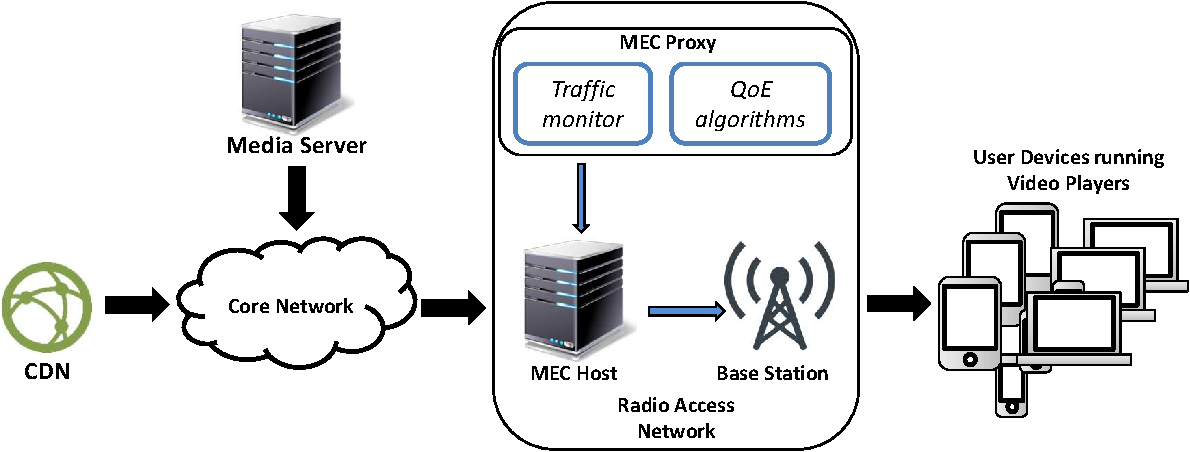
\includegraphics[width=1\textwidth]{architecture_updated.pdf}
	% figure caption is below the figure
	\caption{Architecture of MEC-based QoE estimation approach.}
	\label{fig:MTAP2020architecture} % Give a unique label
\end{figure}

To achieve it, the MEC Proxy is deployed at the MEC Host and monitors all the traffic exchanged at RAN between the video players, media server and CDN \cite{etsigsmec002}. During this operation, it can assess specific metrics related to the streaming session from two different activities:
\begin{itemize}
	\item download of video manifest from media server, which includes different metadata for each representation such as resolutions, nominal bitrates, or language for the different media streams;
	\item player's representation selection, when matching the HTTP segment requests with representations available in the manifest.
\end{itemize}

When a streaming session is started, the MEC Proxy downloads the video manifest and serves it to the player. The MEC Proxy can locally analyse the manifest to list the available representations and their features since the manifest includes information for all the available video, audio and subtitles tracks. Later, when the session is already playing, the video player must retrieve segments from the media server or CDN through HTTP requests. In this case, the MEC Proxy can act in two different ways:
\begin{enumerate}
	\item MEC Proxy can parse the information contained inside the HTTP URL and header as well as obtain request/response timestamps;
	\item MEC Proxy can analyse all the HTTP packets payload, meaning an active analysis of the media stream.
\end{enumerate}

Our solution is on top of first option to reduce the processing demands of the Proxy at the edge and favour a more scalable solution. In any case, it is security/privacy sensitive since standard encryption mechanisms of HAS standards just encrypts the payload of media segments to avoid unauthorized playback, so parsing the media manifest and process the HTTP requests endpoints are allowed.

The general communication is presented in Figure \ref{fig:MTAP2020communication}. First, the HTTP Proxy needs to identify each streaming session to link captured timestamps and QoE factors from each request and response to a specific item to infer its QoE metrics. To achieve it, the MEC Proxy generates a random ID when the first HTTP request from an IP requesting a manifest is received. Therefore, the MEC Proxy maintains a list with all the active streaming sessions. A session is considered expired when no HTTP requests are received during the duration of two segments. Then, inactive sessions are removed from the list.

\begin{figure}[htp]
	\centering
	% Use the relevant command to insert your figure file.
	% For example, with the graphicx package use
	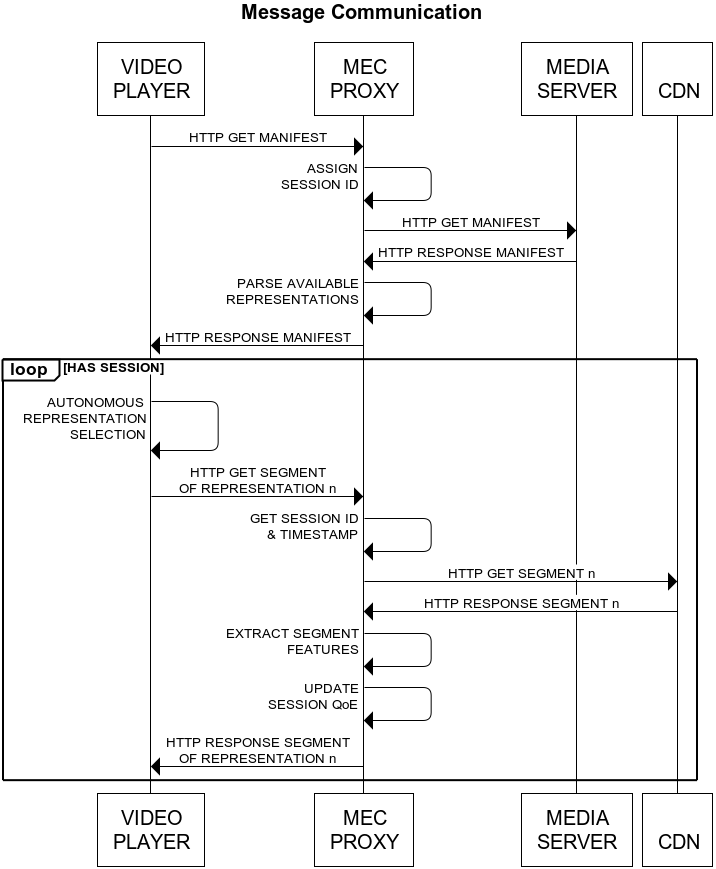
\includegraphics[width=0.8\textwidth]{comms.png}
	% figure caption is below the figure
	\caption{Message communication.}
	\label{fig:MTAP2020communication} % Give a unique label
\end{figure}

When the manifest is received by the video player it decides which representation better fits with the display features, the user preferences, the service subscription, and the network performance. This decision is revised by the video player for each segment to request. Accordingly, it starts to request a specific representation bitrate. The MEC Proxy stores the timestamps to later process request pace to detect any buffering issue when comparing nominal segment duration and time elapsed between requests. Then the MEC Proxy performs the CDN request and analyse some high-level features from the provided segment to accurately estimate the bitrate which may differ from the nominal value declared at the manifest. From that information, the MEC Proxy is can infer an estimated ITU-T P.1203 QoE. Last, the segment is delivered to the video player.

The list of sessions and the estimated QoE, updated for each segment request, is available for other systems at the edge or in the cloud to facilitate the enforcement or enhancement of video streaming in a dense client cell concerning QoE.


\subsubsection{QoE Estimation Algorithm}
\label{sec:MTAP202032}

ITU-T P.1203 \cite{itup1203} describes a model for monitoring media session quality while delivering content through HAS technologies. The building block of the ITU-T P.1203 model is presented in Figure \ref{fig:MTAP2020model}.

\begin{figure}[htp]
	\centering
	% Use the relevant command to insert your figure file.
	% For example, with the graphicx package use
	\includegraphics[width=1\textwidth]{p1203.png}
	% figure caption is below the figure
	\caption{Building blocks of the ITU-T P.1203 model. Source: \cite{itup1203}, Figure 1.}
	\label{fig:MTAP2020model} % Give a unique label
\end{figure}

The ITU-T P.1203 model receives media stream information and playback device features to generates the inputs (\textit{I.11, I.13, I.14, I.GEN}) for the internal modules (\textit{Pa, Pv, Pq, Pav, Pb}). The model generates the following input signals:

\begin{itemize}
	\item I.GEN: Playback display resolution and device type.
	\item I.11: Information on played audio segments, including audio codec and representation features.
	\item I.13: Information on played video segments, including video codec and representation features.
	\item I.14: Stalling event information, including stalling start time and its duration.
\end{itemize}

The inputs may be extracted or estimated in different ways since the ITU-T P.1203 does not provide information on \textit{Buffer parameter extraction} and \textit{Media parameter extraction} modules. The internal modules process the inputs signals to achieve several output QoE scores:
\begin{itemize}
	\item O.21 and O.22: \textit{Pa} and \textit{Pv} modules provide one score per sampling interval for audio and video, respectively.
	\item O.34, O.35 and O.23: \textit{Pav} and \textit{Pb} modules provides cumulative scores for audio-visual and buffering, respectively.
	\item O.46: \textit{Pq} module integrate audio-visual and buffering scores to provide the overall score.
\end{itemize}

All the outputs have 1-5 quality scale, where "1" means "bad" quality and "5" means "excellent" quality, according to MOS specifications \cite{Itu2016}.

The ITU-T P.1203 also establishes 4 modes of operation (mode 0 to 3) \cite{itup1203}. Mode 0 employs only content metadata. All the other modes work only with unencrypted content to acquire information from the media stream. Modes 2 and 3 also require decoding it. Consequently, if we employ mode 1-3 at the MEC Proxy, it may cause security issues. For this reason, we employ mode 0 for our MEC Proxy. Moreover, mode 0 is also the less intensive in terms of processing.

A software implementation of ITU-T P.1203 standard internal modules is provided in \cite{itugithub}. The software implements the internal modules \cite{Robitza2018} according to the ITU-T P.1203 and provides customized \textit{Media parameter extraction} and \textit{Buffer parameter extraction} modules (the ITU-T P.1203 does not specifies these modules). These customized modules are useful to generate compliant inputs signals and evaluate the internal modules, but they are limited for working with locally stored video files. So, they could not be used while streaming a content. All the modules provided by this software implementation are also capable to analyse the media content through any of the four available modes \cite{raake2017}.

To feed the ITU-T P.1203 while streaming a content, we have designed and implemented our custom solutions to generate the inputs. \textit{I.GEN} can be easily known by analysing the header of the HTTP requests since it contains a User-Agent field \cite{useragent} that allows the recognition of the HTTP client type (mobile or desktop device, browser or application, etc.), while keeping anonymous the identity of the user. To extract the remain input signals, we design both \textit{Media parameter extraction} and \textit{Buffer parameter extraction} modules which execute Algorithm \ref{alg:algorithmMedia} and Algorithm \ref{alg:algorithmBuffer}, respectively.

\begin{algorithm}
	\renewcommand{\algorithmicrequire}{\textbf{Input:}}
	\renewcommand{\algorithmicensure}{\textbf{Output:}}
	\caption{Media parameter extraction}
	\label{alg:algorithmMedia}
	\begin{algorithmic}
		\Function{mediaParameter}{Manifest, segment$_n$, \{segment\}$_{n-1}$} \Comment{for each downloaded segment}
		%\parbox[t]{.5\linewidth}{} \linebreak
		\Require Manifest \Comment{media manifest}
		\Require segment$_n$ \Comment{current downloaded segment}
		\Require \{segment\}$_{n-1}$ \Comment{session information including last segment}
		\Ensure \{segment\}$_{n}$ \Comment{session information updated with current segment}
		\State d$_n$, res$_n$, fps$_n$, codec$_n$ $\leftarrow$ parseManifest(Manifest, segment$_n$) \Comment{segment duration, resolution, framerate and codec}
		\State size$_n$ $\leftarrow$ getBitSize(segment$_n$) \Comment{current segment size}
		\State bitrate$_n$ = $\frac{size_n}{d_n}$ \Comment{current segment bitrate}
		\State \{segment$_n$\} = \{d$_n$, res$_n$, fps$_n$, codec$_n$, bitrate$_n$\} \Comment{current segment information}
		\State \{segment\}$_n$ $\leftarrow$ \{\{segment\}$_{n-1}$, \{segment$_n$\}\} \Comment{updated session information}
		\EndFunction
	\end{algorithmic}
\end{algorithm}

The Algorithm \ref{alg:algorithmMedia} is executed for each segment downloaded by the MEC Proxy. It receives the media manifest, the most recent downloaded segment, and the accumulated metadata for the past downloaded segments of a specific session. In the case of employing MPEG-DASH video streaming technology, the manifest would be a Media Presentation Description (MPD). First, specific metadata is captured by matching the manifest and the segment URL, identifying the specific selected representation by the video player for each segment time slot. Second, a more accurate metric in terms of the actual bitrate is captured from the segment size and its nominal duration. Usually, the duration of the segments is fixed as the Group of Pictures (GOP) size is fixed at the encoders to start the segment with a keyframe, so the nominal duration declared in the manifest is accurate. Once all the metadata for the current segment (\{segment$_n$\}) are collected, i.e., bitrate, duration, resolution, framerate and employed codec, this information is stored for all the session long (\{segment\}$_n$), updating the series for the last downloaded segment (\{segment\}$_{n-1}$).

\begin{algorithm}
	\renewcommand{\algorithmicrequire}{\textbf{Input:}}
	\renewcommand{\algorithmicensure}{\textbf{Output:}}
	% \caption{Stall Estimation}
	\caption{Buffer parameter extraction}
	\label{alg:algorithmBuffer}
	\begin{algorithmic}
		% \Function{stallEstimation}{n, d, t$_0$, t$_n$, \{stall\}$_{n-1}$} \Comment{for each downloaded segment}
		\Function{bufferParameter}{n, d, t$_0$, t$_n$, \{stall\}$_{n-1}$} \Comment{for each downloaded segment}
		\Require n \Comment{segment index}
		\Require d \Comment{segment duration}
		\Require t$_0$ \Comment{first segment download time}
		\Require t$_n$ \Comment{current segment download time}
		\Require \{stall\}$_{n-1}$ = \{\{start$^{stall}_0$, d$^{stall}_0$\},...,\{start$^{stall}_k$, d$^{stall}_k$\}\} \Comment{session stalls including last segment}
		\Ensure \{stall\}$_n$ \Comment{session stalls updated with current segment}
		\State $k$ $\leftarrow$ \{stall\}$_{n-1}$ \Comment{number of estimated stalls along the session}
		\State D$^{stall}$ = $\sum_{i=0}^{k}$ d$^{stall}_i$ \Comment{total duration of estimated stalls along the session}
		\State t$_{playback}$ = (t$_n$ - t$_0$) - D$^{stall}$ \Comment{playback time}
		\State d$_{downloaded}$ = (n-1)*d \Comment{total duration of downloaded segments}
		\State d$^{stall}$ = t$_{playback}$ - d$_{downloaded}$ \Comment{candidate stall duration}
		\If {(d$^{stall}$ $>$ 0)} \Comment{check if stalling in the recent segment}
		\State d$_{k+1}^{stall}$ = d$^{stall}$ \Comment{record stall duration}
		\State start$_{k+1}^{stall}$ = t$_n$ - d$^{stall}$ \Comment{stall start time}
		\State \{stall$_{k+1}$\} = \{start$_{k+1}^{stall}$, d$_{k+1}^{stall}$\} \Comment{estimated parameters of new stall (start time and duration)}
		\State \{stall\}$_n$ = \{\{stall\}$_{n-1}$, \{stall$_{k+1}$\}\} \Comment{update stall series}
		\State $k$++ \Comment{new stall when playing the current segment}
		\Else
		\State \{stall\}$_n$ = \{stall\}$_{n-1}$ \Comment{unchanged stall information}
		\EndIf
		\EndFunction
	\end{algorithmic}
\end{algorithm}

The Algorithm \ref{alg:algorithmBuffer} is executed at the MEC Proxy once each segment download is completed by the video player. It estimates stall occurrence and duration without access to video player buffer or playback issues. The MEC Proxy is remotely inferring the playback issues from the timestamps on video player requests. As the video players download a new segment once another has been played, the inter-arrival on video player requests should follow segment duration. Any identified drift likely means a buffering issue. To this end, this function, also executed for each downloaded segment, gets the duration of the segment, the download timestamps of the video player from the segment provided by the MEC Proxy, and the records of past estimations of stalls for previous segment time slots in the session. First, the total duration of estimated stalls along the session is calculated.
Then, the current playback time is measured from the elapsed time from the player's start-up to the last downloaded segment, including the total estimated stall for all the session. The MEC Proxy assumes the first downloaded segment time as the start-up time. It is a reasonable choice since the player starts decoding and displaying the content only when the first segment is completely downloaded. With this assumption, an error could be introduced on the start-up time selection since the proxy cannot measure decoding delay of the first frame. In any case, decoding operation is done in real time, meaning that the maximum error is in the order of tens of milliseconds (1/framerate). Downloading time duration and player's internal buffer size are in the same order of magnitude of segment duration (seconds), which is 100 times higher than the decoding delay. Thus, the error due to decoding delay has a negligible impact on the overall measurement of the start-up time.
To calculate the duration of content available at the video player, the algorithm only includes the previously downloaded segments ($n-1$) excluding the most recent one ($n$). As this function is evaluated just once the segment has been downloaded by the video player, the most recent segment has not been decoded yet. If the current playback time (t$_{playback}$) is lower than the duration of content available at the video player (d$_{downloaded}$), the video player has buffered content to be played, so stall should not happen. If the playback time is ahead the duration of available content, the stall duration is estimated (d$^{stall}$), and the start time of this stall is assumed shifting current segment download time (t$_n$). Last, estimated timestamp and duration of detected stall is stored.

\subsection{Results}

\label{sec:MTAP20204}
\subsubsection{Experimental setup}
\label{sec:MTAP202041}

To demonstrate the effectiveness of the proposed approach to assess the ITU-T P.1203 \cite{itup1203} QoE scores, we deployed the testbed shown in Figure \ref{fig:MTAP2020testbed}. The experimental setup comprises the following:
\begin{itemize}
	\item Media server: we use a mirror server located at Polytechnic University of Turin and belonging to D-DASH dataset and infrastructure \cite{lederer2013} which provides a Dynamic Adaptive Streaming over HTTP (DASH) standard content.
	\item MEC proxy and access point: this is a unique node deployed through a Node.js \cite{nodejs} proxy application running on a Raspberry Pi 3 single-board computer \cite{richardson2012}. Raspberry Pi 3 includes both computing capabilities to execute edge processing and a WiFi internal module to deploy a local wireless network such to provide connection to WiFi clients. Thus, this design guarantees ultra-low latency, proximity and high bandwidth \cite{etsigsmecwifi}. This node has Internet access to download the MPD and the corresponding media segments stored at the Media Server which are served to the clients on demand.
	\item UE node: client node featuring WiFi interface and running several DASH players, based on GStreamer multimedia framework \cite{gstreamer}, which download the video stream. Players run headless (without GUI) since we are not interested in displaying the content and allowing the client to save computing capabilities.
\end{itemize}

% For two-column wide figures use
\begin{figure}[htp]
	\centering
	% Use the relevant command to insert your figure file.
	% For example, with the graphicx package use
	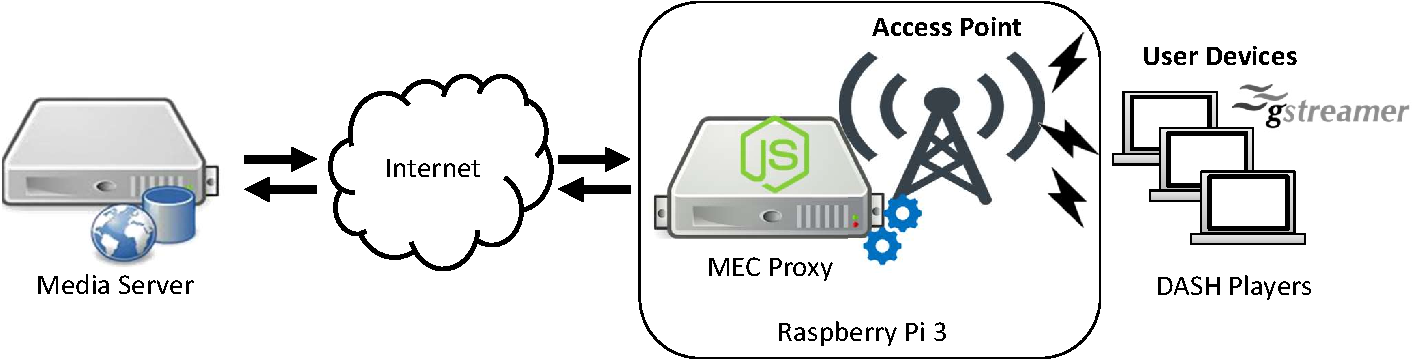
\includegraphics[width=1\textwidth]{testbed_updated.pdf}
	% figure caption is below the figure
	\caption{Testbed.}
	\label{fig:MTAP2020testbed} % Give a unique label
\end{figure}
%

Node.js application at MEC node employs \textit{http-server} module for acquiring HTTP request and response time and \textit{xml2js} module for parsing the MPD to feed Algorithms 1 and 2. During the experiments, Algorithms 1 and 2 are also implemented inside Node.js application and run in real time to generate the inputs of ITU-T P.1203 model. However, ITU-T P.1203 QoE evaluation is performed offline, after that all the metrics are collected. Thus, it simplifies the process of metrics collection and QoE evaluation, while the QoE results remain valid as the input metrics for the ITU-T P.1203 model do not change.

The dataset at the Media Server includes the Red Bull Playstreet video sequence, which is owned by Red Bull Media House and licensed for scientific purposes. This sequence is encoded for 17 video representations through advanced video coding (H.264/AVC) and 4 dual channel audio representations through advanced audio coding (AAC). Both audio and video are segmented with different segment lengths of 2, 4, 6, 10, and 15 seconds, and multiplexed in ISO MPEG4 files (ISO/IEC \hbox{14496-12} - \hbox{MPEG-4} Part 12). For our experiments, we employed 6 seconds segments as such duration favour accuracy of the proposed solution when delivering segments with enough size in bytes to get a more solid assessment of the network performance while downloading, while the serving latency is still valid for streaming of live events.

The representations range from a resolution of 320 x 240 and 30 fps at 100 kbps to a resolution of 1920 x 1080 and 30 fps at 6000 kbps. As the client-side bitrate adaptation mechanism does not target a specific resolution, then each client struggles to achieve the highest representation bitrate.

We use the outcomes of \cite{yu2006} to model players behaviour. The authors provide an extensive analysis on user behaviour while accessing streaming services. The player inter-arrival time fits a modified version of the Poisson distribution. This means that the players are starting and stopping their sessions (joining and leaving the cell/hotspot) along the experiment according to a Poisson distributed inter-arrival time. Moreover, the duration of streaming sessions of the players is variable and follows the declared sections of 5 (37.44\%), 10 (52.55\%), or 25 min (75.25\%). As a result, the effective number of players employed during the experiments is variable since the model is aleatory. Modelling players inter-arrival time and their streaming session duration according to a real distribution allows to emulate a real media traffic scenario.

To test with different network loads, we also consider two different scenarios where we change the limit of the maximum number of concurrent players:

\begin{itemize}
	\item Scenario 1: 10 players at a time. Here, no more than 10 players at a time are connected to the WiFi access node and downloading the content.
	\item Scenario 2: 20 players at a time. The number of players concurrently consuming the video streaming is increased to 20.
\end{itemize}

We perform a test over each scenario for one hour. It results in 66 players taking part in the first scenario and 144 players participating in the second scenario.


%%%%%%%%%%%%%%%%%%%%%%%%%%%%%%%%%%%%%%%%%%%%%%%%%%%%%%%%%%%%%%%%%%%%%%%%%
\subsubsection{Evaluation metrics}
\label{sec:MTAP202042}

To evaluate the proposed solution, we employ the outputs of the ITU-T P.1203, which provide subjective evaluation of the streaming sessions. Since we are focused on evaluating QoE of video representation, we target the following outputs from the ones analysed by ITU-T P.1203:

\begin{itemize}
	\item O.34: it provides a video quality score per output sampling interval. The default interval of the ITU-T P.1203 implementation is 1s, so we have 6 new values per every downloaded segment.
	\item O.23: it provides overall score considering stalling events. We update this value every time the player downloads a new segment.
	\item O.46: it provides overall score overall quality score, considering video and stalling events. We update this value every time the player downloads a new segment.
\end{itemize}

To check the accuracy of the values obtained by the MEC Proxy, we compare the outcomes at the MEC with the outputs at the player side. At the player it is not necessary to design algorithms to extract, estimate or infer the target signals of the ITU-T P.1203 model since all of them are directly available at the video player. The player establishes the video representation, then it knows the features of the downloaded segment after selecting one. Moreover, to know if a stall is experienced, it is enough to check when the internal playback buffer goes empty.

\subsubsection{QoE estimation at the Edge results}
\label{sec:MTAP202043}

\begin{figure}[htp]
	\centering
	\subfloat[]{
		% Use the relevant command to insert your figure file.
		% For example, with the graphicx package use
		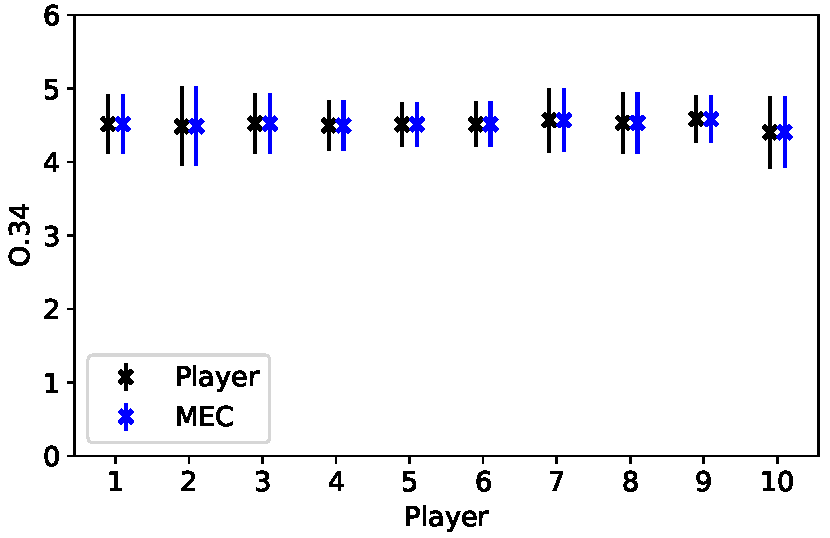
\includegraphics[width=0.6\textwidth]{O34.pdf}
		% figure caption is below the figure
		\label{fig:MTAP2020O34}
	}
	\hfil
	\subfloat[]{
		% Use the relevant command to insert your figure file.
		% For example, with the graphicx package use
		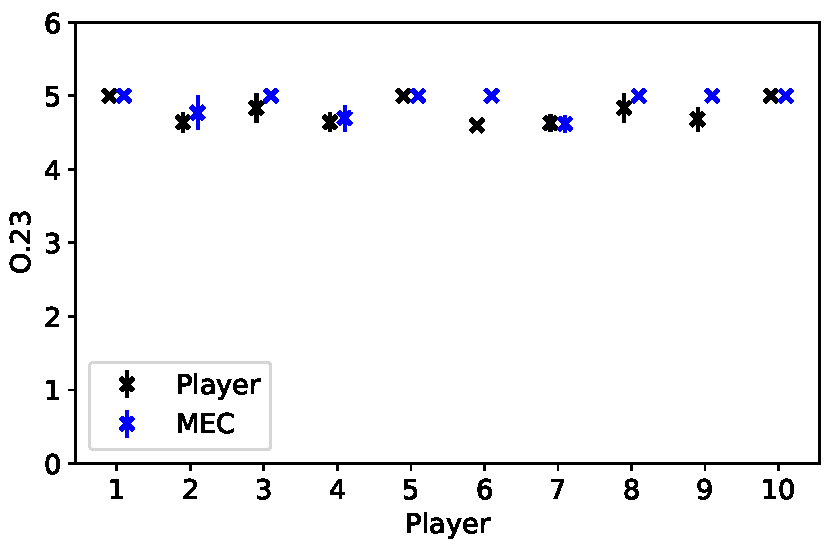
\includegraphics[width=0.6\textwidth]{O23.pdf}
		% figure caption is below the figure
		\label{fig:MTAP2020O23}
	}
	\hfil
	\subfloat[]{
		% Use the relevant command to insert your figure file.
		% For example, with the graphicx package use
		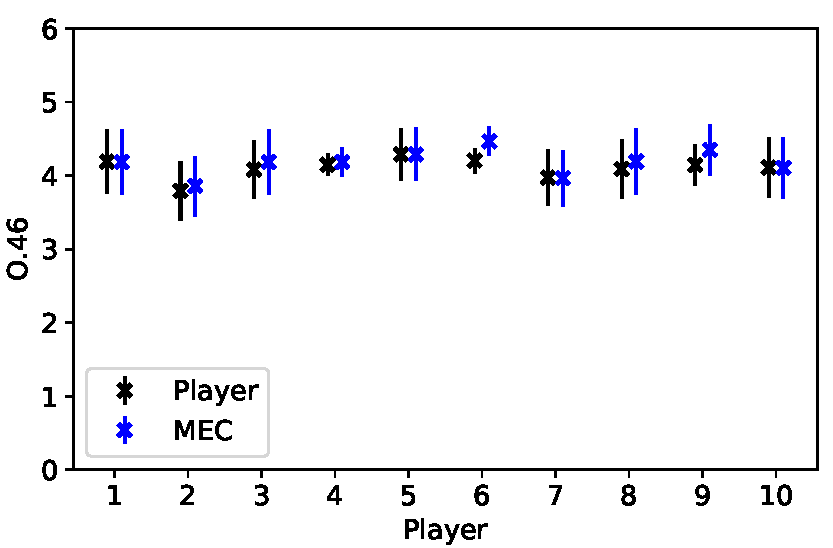
\includegraphics[width=0.6\textwidth]{mos.pdf}
		% figure caption is below the figure
		\label{fig:MTAP2020O46}
	}
	\hfil
	\caption{Average and standard deviation of ITU-T P.1203 QoE scores for 10 players from Scenario 2: O.34 (a), O.23 (b) and O.46 (c).}
	\label{fig:MTAP2020mos} % Give a unique label
\end{figure}

As described in Section \ref{sec:MTAP202041}, the player inter-arrival time and session duration are modelled as described at \cite{yu2006}. While testing the proposed solution for one hour, it resulted in 66 video players for Scenario 1 and 144 for Scenario 2. In terms of computational capabilities consumption, Raspberry Pi 3, which runs the MEC Proxy (Algorithms 1 and 2) and the access point, experiences 13\% CPU and 122MB RAM usage during Scenario 1 and 17\% CPU and 156MB RAM usage during Scenario 2.

\begin{table}[htp]
	\caption{Scenario 1: number (N$_{stall}$) and total duration (T$_{stall}$) of stalls.}
	\centering
	\bgroup
	\def\arraystretch{1.2}%  1 is the default, change whatever you need
	\setlength\tabcolsep{2.5pt} % default value: 6pt
	\label{tab:MTAP2020stall1}
	{\scriptsize
		\begin{tabular}{>{\centering\arraybackslash}m{\dimexpr0.1\textwidth-2\tabcolsep-\arrayrulewidth\relax}
				>{\centering\arraybackslash}m{\dimexpr0.1\textwidth-2\tabcolsep-\arrayrulewidth\relax}
				>{\centering\arraybackslash}m{\dimexpr0.1\textwidth-2\tabcolsep-\arrayrulewidth\relax}
			}
			\toprule
			& \textbf{N$_{\textbf{stall}}$} & \textbf{T$_{\textbf{stall}}$} \\
			\midrule
			\midrule
			\textbf{Player} & 661 & 289s \\
			\textbf{MEC} & 160 & 263s \\
			\bottomrule
			\bottomrule
		\end{tabular}
	}
	\egroup
\end{table}

\begin{table}[htp]
	\caption{Scenario 2: number (N$_{stall}$) and total duration (T$_{stall}$) of stalls.}
	\centering
	\bgroup
	\def\arraystretch{1.2}%  1 is the default, change whatever you need
	\setlength\tabcolsep{2.5pt} % default value: 6pt
	\label{tab:MTAP2020stall2}
	{\scriptsize
		\begin{tabular}{>{\centering\arraybackslash}m{\dimexpr0.1\textwidth-2\tabcolsep-\arrayrulewidth\relax}
				>{\centering\arraybackslash}m{\dimexpr0.1\textwidth-2\tabcolsep-\arrayrulewidth\relax}
				>{\centering\arraybackslash}m{\dimexpr0.1\textwidth-2\tabcolsep-\arrayrulewidth\relax}
			}
			\toprule
			& \textbf{N$_{\textbf{stall}}$} & \textbf{T$_{\textbf{stall}}$} \\
			\midrule
			\midrule
			\textbf{Player} & 1623 & 757s \\
			\textbf{MEC} & 334 & 765s \\
			\bottomrule
			\bottomrule
		\end{tabular}
	}
	\egroup
\end{table}

Figure \ref{fig:MTAP2020mos} shows average value and standard deviation along the streaming session of the considered ITU-T P.1203 outputs. It shows only the results for 10 players randomly chosen among the executed ones of the Scenario 2 since it is the most demanding scenario, where more stalls and quality changes are experienced. Scenario 1 has similar results, but as expected the average values are higher due to the lower competition for the available network resources. The results for O.34 (Figure \ref{fig:MTAP2020O34}) obtained at the MEC are like the ones obtained at the player. It is reasonable since most of the video information to provide to the ITU-T P.1203 model comes from the MPD, which is available at the player, as well as at the MEC Proxy. On the contrary, the results for O.23 (Figure \ref{fig:MTAP2020O23}) shows some differences since the Algorithm \ref{alg:algorithmBuffer} may not detect all the stalling events at the player side from the MEC Proxy. The sampling time to check for stalls at the MEC Proxy is equal to the segment duration. Then, a stall experienced by the player, whose duration is short, and it is recovered before the next check at the MEC, may not be detected correctly. Consequently, estimated values at the MEC are higher that the captured ones at the player. Tables \ref{tab:MTAP2020stall1} and \ref{tab:MTAP2020stall2} also provides more in-depth details of the stalls. It is clear from the tables that the MEC cannot detect all the stalls. Anyway, the total duration of stalls tends to actual one experienced by the player. It means that MEC Proxy cannot detect micro-stalls and tends to concentrate several of them into a macro-stall. Again, this is due to the sampling time to check for stalls. If two micro-stalls are experienced during the same segment, the MEC Proxy will consider that they are one longer stall since it checks only at the end of each segment download. Finally, O.46 scores (Figure \ref{fig:MTAP2020O46}) are directly influenced by the results obtained by the other two scores (O.34 and O.23). It has a significant standard deviation due to video scores (O.34), but lower average value due to the impact of buffering score (O.23).

Tables \ref{tab:MTAP2020results11} and \ref{tab:MTAP2020results12} resume the scores of all the players executed under the Scenarios 1 and 2, respectively. The Tables shows the results by averaging the values obtained by the players and evaluating the standard deviation for each considered score. The Tables confirms that O.34 has the same values when estimated at the MEC and captured at the player, while O.23 scores assessed at the MEC tends to be higher than the real values issued at the player. Again, O.46 scores, which are influenced by the other two scores, shows a standard deviation coming from O.34 and lower average values inherited from O.23.

\begin{table}[htp]
	\caption{Scenario 1: average and standard deviation of ITU-T P.1203 QoE scores.}
	\centering
	\bgroup
	\def\arraystretch{1.2}%  1 is the default, change whatever you need
	\setlength\tabcolsep{2.5pt} % default value: 6pt
	\label{tab:MTAP2020results11}
	{\scriptsize
	\begin{tabular}{>{\centering\arraybackslash}m{\dimexpr0.1\textwidth-2\tabcolsep-\arrayrulewidth\relax}
			>{\centering\arraybackslash}m{\dimexpr0.1\textwidth-2\tabcolsep-\arrayrulewidth\relax}
			>{\centering\arraybackslash}m{\dimexpr0.1\textwidth-2\tabcolsep-\arrayrulewidth\relax}
			>{\centering\arraybackslash}m{\dimexpr0.1\textwidth-2\tabcolsep-\arrayrulewidth\relax}
			>{\centering\arraybackslash}m{\dimexpr0.1\textwidth-2\tabcolsep-\arrayrulewidth\relax}
			>{\centering\arraybackslash}m{\dimexpr0.1\textwidth-2\tabcolsep-\arrayrulewidth\relax}
			>{\centering\arraybackslash}m{\dimexpr0.1\textwidth-2\tabcolsep-\arrayrulewidth\relax}
		}
		\toprule
		& \textbf{O.34$_{\textbf{avg}}$} & \textbf{O.34$_{\textbf{std}}$} & \textbf{O.23$_{\textbf{avg}}$} & \textbf{O.23$_{\textbf{std}}$} & \textbf{O.46$_{\textbf{avg}}$} & \textbf{O.46$_{\textbf{std}}$} \\
		\midrule
		\midrule
		\textbf{Player} & 4.71 & 0.28 & 4.81 & 0.20 & 4.38 & 0.28 \\
		\textbf{MEC} & 4.70 & 0.28 & 4.84 & 0.19 & 4.39 & 0.28 \\
		\bottomrule
		\bottomrule
	\end{tabular}
	}
	\egroup
\end{table}

\begin{table}[htp]
	\caption{Scenario 2: average and standard deviation of ITU-T P.1203 QoE scores.}
	\centering
	\bgroup
	\def\arraystretch{1.2}%  1 is the default, change whatever you need
	\setlength\tabcolsep{2.5pt} % default value: 6pt
	\label{tab:MTAP2020results12}
	{\scriptsize
	\begin{tabular}{>{\centering\arraybackslash}m{\dimexpr0.1\textwidth-2\tabcolsep-\arrayrulewidth\relax}
			>{\centering\arraybackslash}m{\dimexpr0.1\textwidth-2\tabcolsep-\arrayrulewidth\relax}
			>{\centering\arraybackslash}m{\dimexpr0.1\textwidth-2\tabcolsep-\arrayrulewidth\relax}
			>{\centering\arraybackslash}m{\dimexpr0.1\textwidth-2\tabcolsep-\arrayrulewidth\relax}
			>{\centering\arraybackslash}m{\dimexpr0.1\textwidth-2\tabcolsep-\arrayrulewidth\relax}
			>{\centering\arraybackslash}m{\dimexpr0.1\textwidth-2\tabcolsep-\arrayrulewidth\relax}
			>{\centering\arraybackslash}m{\dimexpr0.1\textwidth-2\tabcolsep-\arrayrulewidth\relax}
		}
		\toprule
		& \textbf{O.34$_{\textbf{avg}}$} & \textbf{O.34$_{\textbf{std}}$} & \textbf{O.23$_{\textbf{avg}}$} & \textbf{O.23$_{\textbf{std}}$} & \textbf{O.46$_{\textbf{avg}}$} & \textbf{O.46$_{\textbf{std}}$} \\
		\midrule
		\midrule
		\textbf{Player} & 4.53 & 0.31 & 4.76 & 0.19 & 4.22 & 0.27 \\
		\textbf{MEC} & 4.53 & 0.31 & 4.85 & 0.20 & 4.28 & 0.28 \\
		\bottomrule
		\bottomrule
	\end{tabular}
	}
	\egroup
\end{table}

As expected, Scenario 1 presents higher values for any of the considered metrics since the network resources are the same as Scenario 2, but the number of players sharing them is lower. The resulting standard deviations are similar for both scenarios.

Tables \ref{tab:MTAP2020results21} and \ref{tab:MTAP2020results22} compare the results obtained at the MEC and at the player side by providing the Mean Absolute Error (MAE) and Root Mean Square Error (RMSE) between the different scores. The results show that the scores obtained at the MEC tends to be like the ones obtained at the player, achieving more accurate results in the Scenario 1, as expected.

\begin{table}[htp]
	\caption{Scenario 1: MAE and RMSE for ITU-T P.1203 QoE scores.}
	\centering
	\bgroup
	\def\arraystretch{1.2}%  1 is the default, change whatever you need
	\setlength\tabcolsep{2.5pt} % default value: 6pt
	\label{tab:MTAP2020results21}
	{\scriptsize
	\begin{tabular}{>{\centering\arraybackslash}m{\dimexpr0.1\textwidth-2\tabcolsep-\arrayrulewidth\relax}
			>{\centering\arraybackslash}m{\dimexpr0.1\textwidth-2\tabcolsep-\arrayrulewidth\relax}
			>{\centering\arraybackslash}m{\dimexpr0.1\textwidth-2\tabcolsep-\arrayrulewidth\relax}
			>{\centering\arraybackslash}m{\dimexpr0.1\textwidth-2\tabcolsep-\arrayrulewidth\relax}
		}
		\toprule
		& \textbf{O.34} & \textbf{O.23} & \textbf{O.46} \\
		\midrule
		\midrule
		\textbf{MAE} & 0.21 & 0.11 & 0.18 \\
		\textbf{RMSE} & 0.39 & 0.21 & 0.36 \\
		\bottomrule
		\bottomrule
	\end{tabular}
	}
	\egroup
\end{table}

\begin{table}[htp]
	\caption{Scenario 2: MAE and RMSE for ITU-T P.1203 QoE scores.}
	\centering
	\bgroup
	\def\arraystretch{1.2}%  1 is the default, change whatever you need
	\setlength\tabcolsep{2.5pt} % default value: 6pt
	\label{tab:MTAP2020results22}
	{\scriptsize
	\begin{tabular}{>{\centering\arraybackslash}m{\dimexpr0.1\textwidth-2\tabcolsep-\arrayrulewidth\relax}
			>{\centering\arraybackslash}m{\dimexpr0.1\textwidth-2\tabcolsep-\arrayrulewidth\relax}
			>{\centering\arraybackslash}m{\dimexpr0.1\textwidth-2\tabcolsep-\arrayrulewidth\relax}
			>{\centering\arraybackslash}m{\dimexpr0.1\textwidth-2\tabcolsep-\arrayrulewidth\relax}
		}
		\toprule
		& \textbf{O.34} & \textbf{O.23} & \textbf{O.46} \\
		\midrule
		\midrule
		\textbf{MAE} & 0.14 & 0.14 & 0.19 \\
		\textbf{RMSE} & 0.43 & 0.24 & 0.36 \\
		\bottomrule
		\bottomrule
	\end{tabular}
	}
	\egroup
\end{table}

Note that O.34 has higher MAE and RMSE than O.23 and O.46. It could be considered a contradictory to the fact that the values obtained at MEC Proxy compared to the values captured at the player for O.34 are more accurate than O.23 and O.46. Anyway, it is important to remember that these metrics have different sampling rates. O.34 provides a value every second, while O.23 and O.46 every segment (6s). Then, O.34 has higher values for MAE and RMSE since they are evaluated over a number of scores which is 6 times bigger than O.23 and O.46. Finally, if we compare the two scenarios, the results tend to be similar since the MAE and RMSE are relative values, they are not conditioned by the average values of the metrics. It means that the MEC Proxy performs similarly in both scenarios.

In summary, the proposed MEC Proxy can monitor network dynamics and estimate the individual QoE of each player according to Recommendation ITU-T P.1203. The results show that video related scores (O.34) estimated follow the actual ones captured at the player, while buffering scores (O.23) tend to miss some small stalls unperceived from segment to segment. Anyway, the overall scores (O.46) are still valid showing a small difference of the estimated values at the MEC from the actual values captured at the player.

\subsection{Conclusion}
\label{sec:MTAP20205}

The trend for the following years is an increasing consumption of media content due to the popularity of video streaming platforms. To cope with this increasing demand, MNOs need to manage the network according to cost-effective policies, requiring monitoring solutions which provide actionable data to management systems to provide the best QoE with the available network resources.

The proposed 5G MEC-enabled proxy aims to estimate the ITU-T P.1203 QoE metrics to enable edge services operating coordinated decisions on the streaming qualities. The MEC Proxy assesses QoS metrics at the radio cell and parses manifests of requested DASH streams to estimate the parameters employed to evaluate ITU-T P.1203 QoE scores. Consequently, there is no need for explicit out-of-band messaging from video players to send playback statistics to the MEC.

The solution has been implemented in a real testbed where WiFi was employed as access network between MEC and players and tested in two scenarios with different demands and traffic loads over the network. The results demonstrate the capability of the MEC Proxy to estimate ITU-T P.1203 QoE scores close to actual ones.

\subsection*{Acknowledgment}
This work was fully supported by the 5G-TEST project (Gipuzkoa's research and innovation programme) and Open-VERSO project (Red Cervera program, Spanish government's Centre for the Development of Industrial Technology).
		

% !TeX spellcheck = en_US
%Publications.tex
%\newcommand{\PublicationsPath}{PatentsAndPublications/Publications}

%BMSB2018

\section[MEC Proxy for efficient cache and reliable multi-CDN video distribution]{MEC Proxy for efficient cache and reliable multi-CDN video distribution}
\label{chap:BMSB2018}
\begin{itemize} \itemsep1pt\parskip0pt\parsep0pt
	\item \textbf{Title:} MEC Proxy for efficient cache and reliable multi-CDN video distribution
	\item \textbf{Authors:} Roberto Viola, \'Angel Mart\'in, Mikel Zorrilla and Jon Montalb\'an
	\item \textbf{Proceedings:} 2018 IEEE International Symposium on Broadband Multimedia Systems and Broadcasting (BMSB)
	\item \textbf{Publisher:} IEEE
	\item \textbf{Year:} 2018
	\item \textbf{DOI:}  \url{10.1109/BMSB.2018.8436904}
\end{itemize}	

\textbf{Abstract:} The massive consumption of media contents needs of network accelerators, which boost the media delivery and optimize the traffic volume crossing the network from servers to media players. Content Delivery Network (CDN) is the common network function to distribute in a cloud-manner the contents, enhancing media availability and distribution performance. However, high concurrency rates of media sessions can produce CDN performance degradations and outages that impact negatively the Quality of Experience (QoE). 5G Multi-access Edge Computing (MEC) architecture envisions a QoE-aware system at the network edge which performs analytics to enhance or boost media services. This paper provides a novel MEC proxy to expand and enforce caching infrastructures for efficient and reliable content distribution. First, the proxy caches contents on the network edge to reduce the Capital Expenditure (CAPEX) of the CDN for the OTT service provider. To this end, the proxy is able to identify recurrent requests. Second, the proxy shields from identified or predicted CDN malfunction. Here, the proxy switches the download sessions to an alternative CDN in order to ensure QoE rates, enabling a CDN dynamic selection based on live connectivity statistics. The proposed solution is evaluated by delivering Dynamic Adaptive Streaming over HTTP (MPEG-DASH) streams in a dense client cell while applying different caching strategies.

\textbf{Keywords:} 5G, CDN, distributed cache, MEC, QoE, reliability \& streaming analytics.	
	
	
\subsection{Introduction}

The increase of video streaming users and the service requirements are driving the evolution of media services over the Internet. Mobility and quality improvements are the key catalysers in this evolution. Cisco estimates that video traffic will cover the 82\% of all Internet traffic by 2021 \cite{ciscovideo2016}. Moreover, mobile traffic growth is estimated to be twice as fast as fixed IP traffic from 2016 to 2021 \cite{ciscomobile2016}.

The delivery performance from the network has a big impact on the perceived QoE of the end user of media services. However, video streaming services work on top of unmanaged networks, where the traffic is managed and forwarded on a best-effort basis \cite{sodagar2011mpeg}. This operational context is targeted by the video streaming solution MPEG-DASH. MPEG-DASH inherits many benefits from Hypertext Transmission Protocol (HTTP). First, it enables a pull-based streaming \cite{begen2011} to easily traverses network functions such as firewalls and NAT devices. Second, MPEG-DASH streams can be played anywhere as any connected device supports HTTP. Third, MPEG-DASH has a Content Delivery Network (CDN)-ready design enabling the exploitation of existing HTTP caching infrastructures, which enhance the availability and the responsiveness of the content distribution.

Beyond the current network functions to boost and enhance the traffic delivery, the capacity and performance promised by 5G networks will make a significant leap towards higher data rates, heavier user densities and ultra-reliable and low-latency communications. The European Telecommunications Standards Institute (ETSI) specifies a set of component technologies which will be essential part of 5G systems, such as, Network Functions Virtualization (NFV), Millimetre Wave Transmission (mWT), Next Generation Protocols (NGP) and Multi-access Edge Computing (MEC) \cite{etsi2019}. MEC architecture allows Mobile Network Operators (MNOs) to supply video delivery analytics-based intelligence at the network edge. Thus, MEC plays a significant role to achieve specific media traffic goals with zero-latency in a distributed manner. Furthermore, MEC enables coordinated operations at the network edge such to be transparent to the media server and players.

This work proposes a novel network proxy, called MEC4CDN, which complies with MEC architecture. MEC4CDN provides two features. First, it performs a local cache of identified trending contents to minimize the traffic between the CDN and the network edge. Second, it applies a dynamic selection of the CDN based on live measurements in the context of a multi-CDN delivery. The proposed solution allows the client to start playing from a CDN, that is favourable in terms of Quality of Service (QoS), and transparently and dynamically switch to another one which provides better performance in case of CDN degradation or outage. To this end, the proxy collects and process L3 connectivity metrics, L7 MPEG-DASH Media Presentation Description (MPD) files and L7 QoE scores. So, the proxy handles multiple CDN endpoints, deciding to locally cache a response for near future requests, or to conduct the request to a healthy cloud CDN in case of detected issues.

The paper is structured as follows. First, section \ref{sec:BMSB2018related} reviews the related work to improve the network delivery. Then, section \ref{sec:BMSB2018multi-CDN} describes the proposed MEC4CDN network proxy. Section \ref{sec:BMSB2018implementation} presents the implementation of the solution. To validate the solution, section \ref{sec:BMSB2018results} compiles the testbed and the results. Finally, section \ref{sec:BMSB2018conclusion} gathers the conclusions of this work.

\subsection{Related Work}
\label{sec:BMSB2018related}

Apart from the content catalogue, the Quality of Experience (QoE) is a key aspect for user satisfaction and retention when rating streaming services. Hence, any system trying to enhance media delivery needs to consider QoE metrics.

QoS assesses the network delivery performance and it has a direct impact on human perception QoE. In this sense, stability of media playback is related to efficient utilization and fair resource sharing. Nevertheless, these key aspects are not guaranteed in unmanaged networks. This situation may lead to suboptimal results in terms of video playback, link utilization, and fairness among the clients \cite{chen2016}. 

Specific metrics for QoE of HTTP-based adaptive media streaming services, such as initial delay, stalling time, number of quality switches and inter-switching times, are fundamental parameters to get the estimated Mean Opinion Score (eMOS) \cite{claeys2014}. This model quantifies the quality of video streaming services without a demographic perception study. Recently, the work \cite{lentisco2017} investigates a new model for MOS, called Ubiquitous-Mean Opinion Score for Video (U-vMOS), which makes initial buffering more dominant than \cite{claeys2014} model.

Caching is a common technique to get enhanced QoE for massive content consumption services. The CDN is the traditional network function provisioning cache features as a cloud service. Fueled by the CDN vendor proliferation, media services employ multi-CDN strategies to get a more reliable and cost-effective content delivery. Netflix case, as an example of multi-CDN solution, is studied in \cite{adhikari2012}. More recent work \cite{adhikari2015} also includes Hulu analysis for 3 CDN vendors. Here, with alternative CDNs available, the employed CDN is set by the streaming service for each session, where the choice is done by the server. This centralized architecture is difficult to scale hampering the orchestration of common policies or decisions to all users in an area.

When the employed CDN is not pre-set, transferring to clients the possibility to dynamically choose, each client should analyze repeatedly the network performance of each CDN. It means the introduction of a network overhead proportional to the number of clients and the number of CDNs. Hence, a client-side CDN selection is not an optimal solution.

Consequently, the European Broadcasting Union (EBU) aims to avoid both pre-set CDN and client's CDN selection by proposing the EBU Flow Multi-CDN \cite{EurovisionFLOW}. It consists in a CDN switching service which selects the optimal CDN at any given moment in time. A similar solution is also provided by Cedexis Multi-CDN \cite{cedexis}. Both EBU and Cedexis proposals monitor network analytics at core network, then they are not aware of the state of connected clients at network edge.

On the contrary, if we focus at the network edge, the access point has knowledge of both the connected clients' activity in its cell and the CDN performance from its location. A proxy located at the network edge, retrieving access point information, can evaluate the performance of the delivery network just once and exploit it for each client (independently from the number of clients in the cell). This perfectly suits the telecommunication industry which proposes MEC as a new functional architecture to be integrated on the mobile network infrastructure. MEC allows Internet service provider (ISP) to provide Information Technology (IT) and cloud computing services at the edge of the network, closer to the clients. Hence, MEC opens the door for authorized Content Providers (CPs) to develop their own applications hosted on the MEC server. Therefore, CPs are able to tune the behavior of content delivery to end users in 4G and 5G contexts. Furthermore, next generation networks and 5G MEC architecture enable the deployment of distributed local caches at the network edge to efficiently minimize the volume of traffic passing through the network core and backhaul.

\subsection{MEC Proxy for Multi-CDN Delivery}
\label{sec:BMSB2018multi-CDN}

The proposed MEC4CDN proxy server, located on a MEC component, can exploit the knowledge of network analytics of different delivery paths. It aims to improve the overall throughput while minimizing the latency, in an environment where multiple clients are competing for network resources. 

Figure \ref{fig:BMSB2018selection} shows a scenario where a content is provided by means of two CDN vendors. For some reasons, such as sudden massive connections or geo-based cycles of human activity, the performance of \textit{CDN A} starts to degrade. At the same time, the capacity of \textit{CDN B} is improved because the \textit{CDN B} starts to provision more resources for a specific area. The MEC4CDN system gets awareness of this unbalanced situation, based on L3 stats, and orchestrates all the media players subscribed to the managed cell to dynamically employ a CDN which ensures better QoS. 

\begin{figure}[htp]
	\centering
	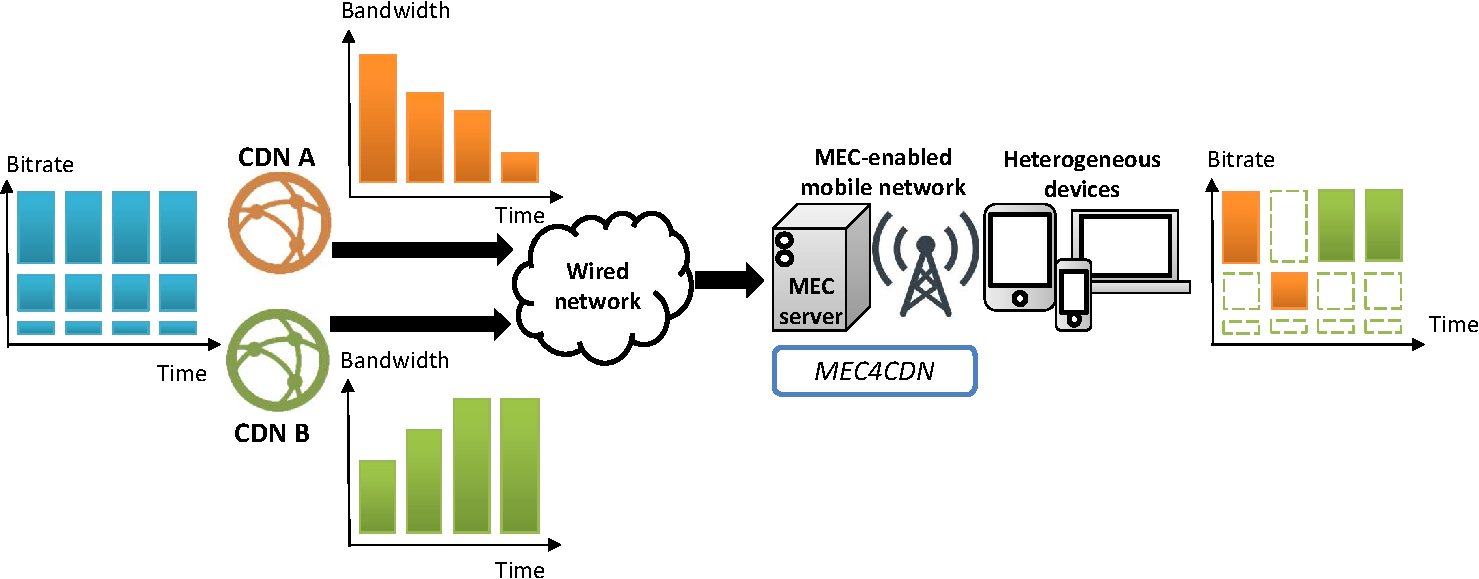
\includegraphics[width=1\textwidth,keepaspectratio]{selection.pdf}
	\caption{MEC4CDN multi-CDN selection.}
	\label{fig:BMSB2018selection}
\end{figure}

Therefore, for services delivered over multiple CDN providers, MEC4CDN can select an appropriate CDN for a RAN geo-position in real-time, according to L3 metrics. To this end, MEC4CDN gets alternative CDNs set from the MPD file, provided that it contains multiple definitions of \textit{base URL} storing the path to the CDNs, or from the media service. Then, MEC4CDN employs the set of CDNs to dynamically switch the base URL of media sessions in the same RAN when necessary. So, in case of detected performance degradation, the MEC4CDN system replaces the base URL field of all the managed sessions to another known CDN endpoint, migrating all the managed clients at once to avoid outages.

The sequence diagram with the exchanged messages to allow the CDN switching is depicted in Figure \ref{fig:BMSB2018sequence_cdn}. First, the MEC proxy server running MEC4CDN captures the HTTP GET requests from the User Equipments (UEs) to download the MPD file from the media server. Then, MEC4CDN retrieves the MPD file from the media server and appropriately parses it in order to retrieve the \textit{base URLs} set before sending it to the UE. Then, the UE selects a representation bitrate ($R_j$) from the available ones according to display resolution, user preferences and connection capacity stats. The UE requests, through the MEC proxy, a specific segment file to the CDN accordingly. Once the MEC proxy server detects the HTTP GET requests from the UEs for downloading a segment file, it retrieves wired path stats. When network performance is not enough, the MEC4CDN switches the \textit{base URL} field of the MPD file applicable for the next segment requests. Such operations are executed at the stream start and each time that the UEs asks for a new segment.

\begin{figure}[htp]
	\centering
	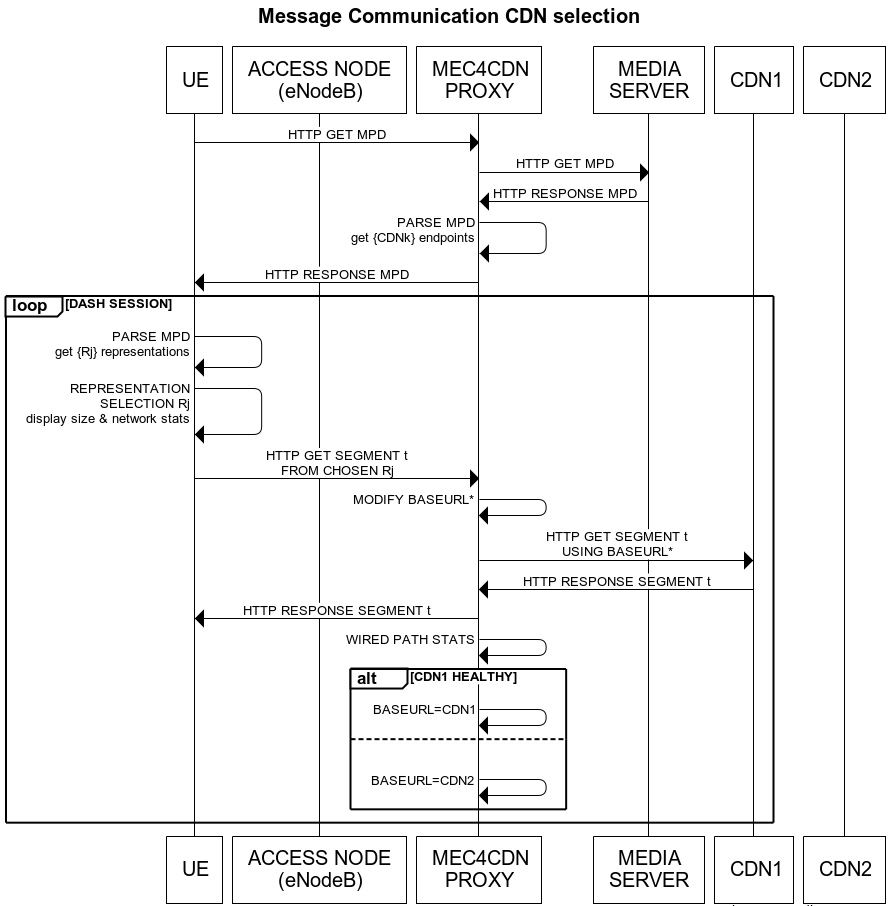
\includegraphics[width=1\textwidth,keepaspectratio]{sequence_cdn_healthy.png}
	\caption{MEC4CDN multi-CDN sequence diagram.}
	\label{fig:BMSB2018sequence_cdn}
\end{figure}

Furthermore, MEC4CDN ships the ability to significantly reduce the CDN traffic for a live content distribution in dense client cells, as depicted in Figure \ref{fig:BMSB2018cache}. In a live media consumption scenario, each UE makes a request to get the video from a CDN. When MEC4CDN comes into play, it performs a local cache at the network edge in a proactive manner. Triggered by the first content request, MEC4CDN downloads all the next segment representations from the CDN. Then, all the following requests are already downloaded and available in the MEC4CDN local cache for any representation bitrate chosen by the media players. Then, the greater the number of clients consuming a live content in a cell, the higher efficiency of this solution.

\begin{figure}[htp]
	\centering
	\subfloat[]
	{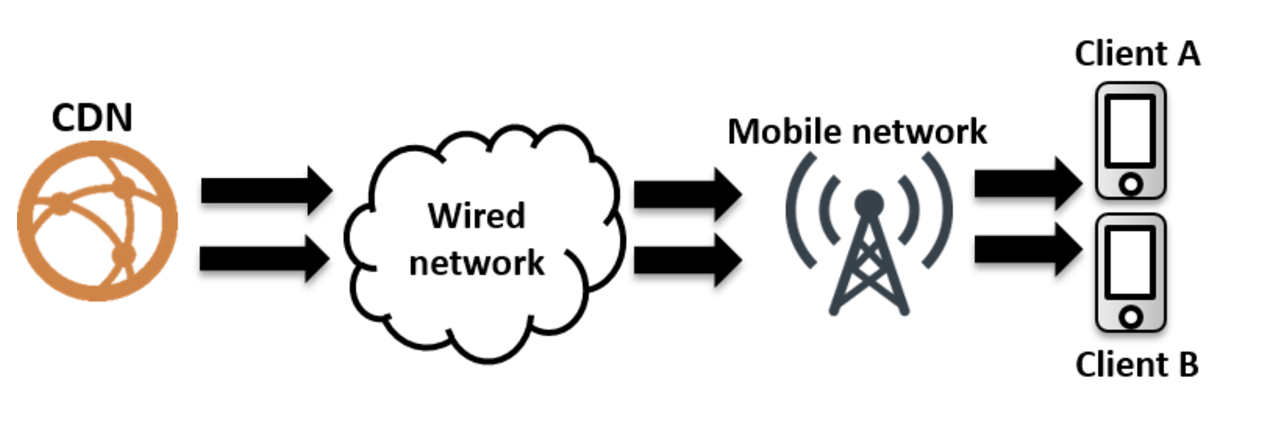
\includegraphics[width=0.8\textwidth,keepaspectratio]{legacy-cache.eps}
		\label{fig:BMSB2018legacy-cache}
	}
	\hfil
	\subfloat[]
	{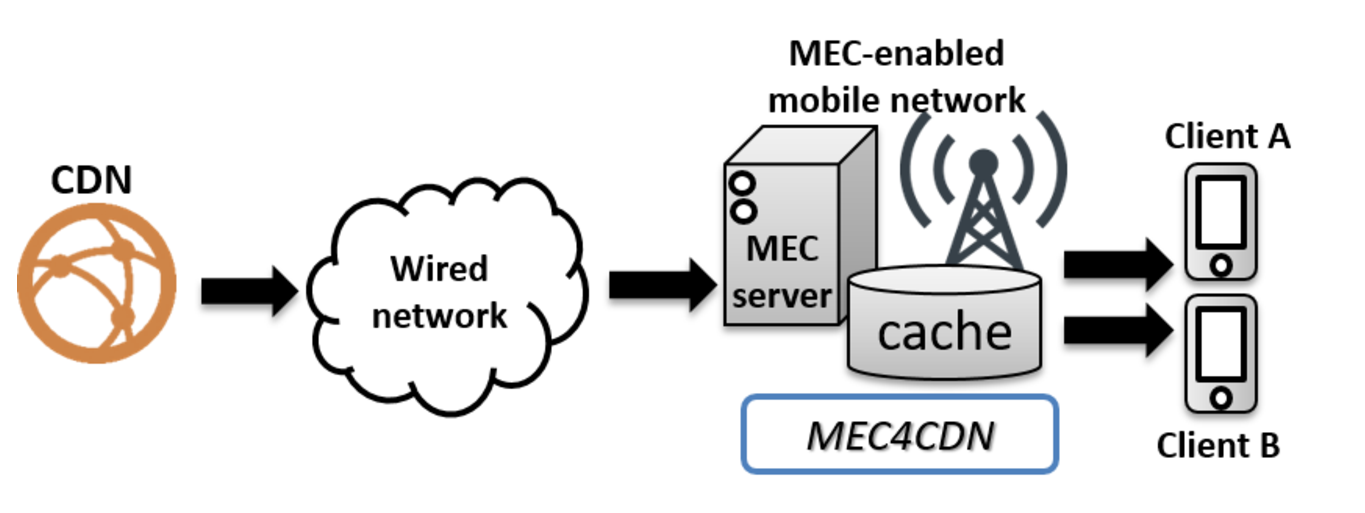
\includegraphics[width=0.8\textwidth,keepaspectratio]{cache.eps}
		\label{fig:BMSB2018cache}
	}
	\hfil
	\caption{Legacy content delivery (a) and MEC4CDN cache-powered delivery (b).}
\end{figure}


The utilization of a CDN means a significant operational cost for media services. Moreover, when massive connections come concurrently to a CDN, the CDN infrastructure can start to collapse and the QoS could be negatively impacted. To prevent media delivery from this situation, it is necessary to turn broadcast of live content into an efficient distribution. To this end, MEC systems located at the network edge can cache recurrent contents, such as live sports events or concerts, in a proactive manner. Cache at network edge can improve the streaming experience caching all available representations. Thus, the selected representation will be locally available for any number of subscribers in a cell, enabling the video to start faster and reducing the buffering time, while minimizing CDN traffic. This approach preserves media players ability to decide the bitrate that fits with their contexts independently.

The sequence diagram with the exchanged messages to allow the local cache of a popular or live content is depicted in Figure \ref{fig:BMSB2018sequence_cache}. The proxy waits for a media content request and proceeds to download all the available representations. Then, the media players in the cell will select a specific representation ($R_j$) according to the device features, the assessed available bandwidth, the user preferences and subscription plan. Once the players start to request a representation for a specific time ($t$), the proxy requests the next segments ($Segments_{t+1} \forall R_j$) to be ready for the following requests.

\begin{figure}[htp]
	\centering
	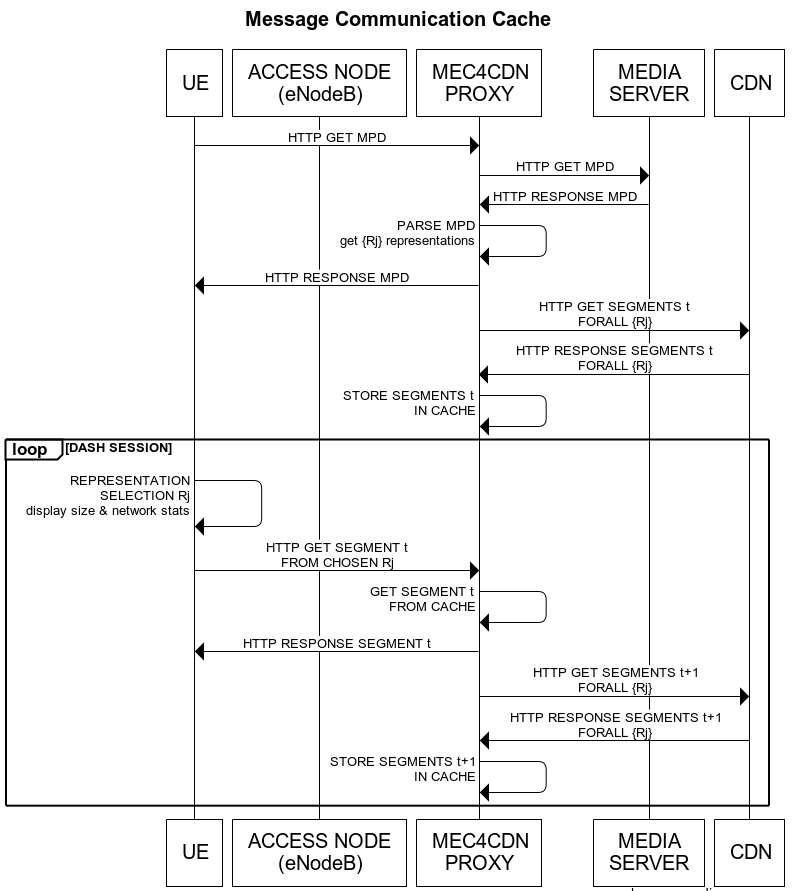
\includegraphics[width=1\textwidth,keepaspectratio]{sequence_cache.png}
	\caption{MEC4CDN cache sequence diagram.}
	\label{fig:BMSB2018sequence_cache}
\end{figure}

It is also important to remark the zero-latency and distributed performance features by design coming from the MEC architecture fundamentals. The MEC systems are distributed and autonomously empower specific services for the co-located cell.

\subsection{Implementation}
\label{sec:BMSB2018implementation}

\makeatletter
\newlength{\trianglerightwidth}
\settowidth{\trianglerightwidth}{$\triangleright$~}
\algnewcommand{\LineComment}[1]{\Statex \hskip\ALG@thistlm $\triangleright$ #1}
\algnewcommand{\LineCommentCont}[1]{\Statex \hskip\ALG@thistlm%
	\parbox[t]{\dimexpr\linewidth-\ALG@thistlm}{\hangindent=\trianglerightwidth \hangafter=1 \strut$\triangleright$ #1\strut}}
\renewcommand{\ALG@beginalgorithmic}{\small}
\makeatother

The program of MEC4CDN for CDN selection is described in Algorithm \ref{alg:BMSB2018algorithmCDN}. The outcome of MEC4CDN is to identify violations of bandwidth or latency performance in order to perform reactive switching to an alternative CDN provider. The inputs of the algorithm are the RTT and the bandwidth from the MEC4CDN proxy to the CDN and the current number of media playing sessions to this CDN. The output is the base URL field of the updated MPD file to be used by the media player.

\begin{algorithm}
	\renewcommand{\algorithmicrequire}{\textbf{Input:}}
	\renewcommand{\algorithmicensure}{\textbf{Output:}}
	\caption{CDN health check to switch all sessions at eNodeB}
	\label{alg:BMSB2018algorithmCDN}
	\begin{algorithmic}
		
		\Procedure{CDNcheck}{ } \Comment{\parbox[t]{.30\linewidth}{listen to requests \& switch CDN}}
		\State rtt$_{max}$ \Comment{setup maximum latency}
		\State CDN$_{list}$ \Comment{set of alternative CDNs}
		\State n$_{p}$ \Comment{number of players}
		\ForAll {segment request} \Comment{from the UE}
		\State SegmentRequest() \Comment{to the CDN$_\textit{k}$}
		\State s$_{CDN_\textit{k}}$ $\leftarrow$ SegmentResponse() \Comment{from the CDN$_\textit{k}$}
		\State rtt$_{CDN_\textit{k}}$ $\leftarrow$ rtt(s$_{CDN_\textit{k}}$) \Comment{L3 latency}
		\State bw$_{CDN_\textit{k}}$ $\leftarrow$ 2$\frac{size(s_{CDN_\textit{k}})}{rtt(s_{CDN_\textit{k}})}$ \Comment{L3 BW}
		\State R$_{max}^{bitrate}$ $\leftarrow$ parse(MPD) \Comment{\parbox[t]{.25\linewidth}{maximum representation bitrate}}
		\If {(rtt$_{CDN_\textit{k}}$ $>$ rtt$_{max}$) $||$ (bw$_{CDN_\textit{k}}$ $<$ (n$_{p}$ x R$_{max}^{bitrate}$))} 
		\State \Comment{insufficient performance}
		\State baseURL $\leftarrow$ alternative(CDN$_{list}$,$CDN_{k}$)
		\State \Comment{change CDN}
		\EndIf
		\EndFor
		\EndProcedure
	\end{algorithmic}
\end{algorithm}

Moreover, the program of MEC4CDN for local cache is described in Algorithm \ref{alg:BMSB2018algorithmCache}. The outcome of MEC4CDN is to proactively download what the users will play in order to locally cache next segments before the player needs to play them, enabling the video to start faster, decreasing stalls, reducing CDN traffic and enhancing the quality of experience. Thus, MEC4CDN reduces resource usage coming from the CDN provider by caching requested contents and exploiting their recurrent likelihood. The inputs of the algorithm are the current segment index employed by the media player and the available representations. The result is the temporal storage of next segments to be requested beyond the current one played by the user.

\begin{algorithm}
	\renewcommand{\algorithmicrequire}{\textbf{Input:}}
	\renewcommand{\algorithmicensure}{\textbf{Output:}}
	\caption{Cache proxy at eNodeB}
	\label{alg:BMSB2018algorithmCache}
	\begin{algorithmic}
		
		\Procedure{LocalCache}{ } \Comment{\parbox[t]{.27\linewidth}{listen to requests \& cache segments}}
		\State i$_{t}$ \Comment{current segment index}
		\State \{R$_{j}$\} \Comment{set of alternative representations}
		\ForAll {R$_j$ $\in$ \{R$_{j}$\}} \Comment{download next segment}
		\State s$_{i_{t}+1}$ $\leftarrow$  Download(i$_{t}+1$,R$_j$) \Comment{from the CDN}
		\State Cache(s$_{i_{t}+1}$,R$_j$) \Comment{at eNodeB proxy}
		\EndFor
		\EndProcedure
		
	\end{algorithmic}
\end{algorithm}


\subsection{Results}
\label{sec:BMSB2018results}

In order to test MEC4CDN solution, we deploy an experimental setup by exploiting a MPEG-DASH distributed dataset described by Lederer et al. \cite{lederer2013} and provided for public experimentation of CDN-like infrastructures. This dataset consists in Red Bull Playstreet sequence stored at several geographically distributed mirror servers. The content is provided in 17 video representations encoded in H.264 Advanced Video Coding (H.264/AVC) and 4 dual channel audio representations encoded in Advanced Audio Coding (AAC). Both audio and video are segmented with different segment lengths of 2, 4, 6, 10, and 15 seconds and multiplexed in ISO MPEG4 files (ISO/IEC 14496-12 - MPEG-4 Part 12).

\begin{table}[htp]
	\caption{Set of MPEG-DASH representations employed in the experiments.}
	\centering
	\bgroup
	\def\arraystretch{1.2}%  1 is the default, change whatever you need
	\setlength\tabcolsep{2.5pt} % default value: 6pt
	\label{tab:BMSB2018reps}
	{\scriptsize
		\begin{tabular}{>{\centering\arraybackslash}m{\dimexpr0.1\textwidth-2\tabcolsep-\arrayrulewidth\relax}
				>{\centering\arraybackslash}m{\dimexpr0.15\textwidth-2\tabcolsep-\arrayrulewidth\relax}
				>{\centering\arraybackslash}m{\dimexpr0.15\textwidth-2\tabcolsep-\arrayrulewidth\relax}
				>{\centering\arraybackslash}m{\dimexpr0.15\textwidth-2\tabcolsep-\arrayrulewidth\relax}
			}
			\toprule
			\textbf{index} & \textbf{bitrate} & \textbf{resolution} & \textbf{framerate} \\
			\midrule
			\midrule
			1 & 400kbps & 480x360 & 30fps  \\
			2 & 900kbps & 854x480 & 30fps  \\
			3 & 1500kbps & 1280x720 & 30fps \\
			4 & 2000kbps & 1280x720 & 30fps \\
			5 & 2500kbps & 1280x720 & 30fps \\
			6 & 3000kbps & 1920x1080 & 30fps \\
			\bottomrule
			\bottomrule
		\end{tabular}
	}
	\egroup
\end{table}

Then, the overall experimental setup comprises both public network nodes and internal ones belonging to our network infrastructure:
\begin{itemize}
	\item Three mirror servers: network nodes provided by Lederer et al. \cite{lederer2013} which we use as CDN-like nodes for storing the media segments.
	\item A media server: a server in our infrastructure storing the MPD file which is requested by the client to play the content.
	The MPD file provides information for the player to retrieve the segments from the mirror servers. Moreover, the service employs segments with duration of 6 seconds and the video content is limited to six different representations, widely used by market services. Each representation is characterized by a specific bitrate as shown in Table \ref{tab:BMSB2018reps}.
	\item A proxy server running MEC4CDN: a server in our infrastructure provided by public Internet connection and acting as a network gateway for the wireless network edge deployed inside our infrastructure. Then, all the requests from the players are processed by the proxy server before being transmitted, if necessary, to the media infrastructures on Internet. It executes the proposed MEC4CDN solution. 
	\item A wireless access point: in order to provide wireless capabilities, an access point is used, which provides a wireless local area network (WLAN) using 2.4Ghz band. The access point is directly connected to the proxy server to provide a MEC-like architecture. The only role of the access point consists in forwarding all the incoming traffic on both directions (download and upload).
	\item A UE running MPEG-DASH players: a wireless network node connected to the access point, which is running GStreamer MPEG-DASH players.
\end{itemize}
The experimental setup is shown in Figure \ref{fig:BMSB2018testbed}.

\begin{figure}[htp]
	\centering
	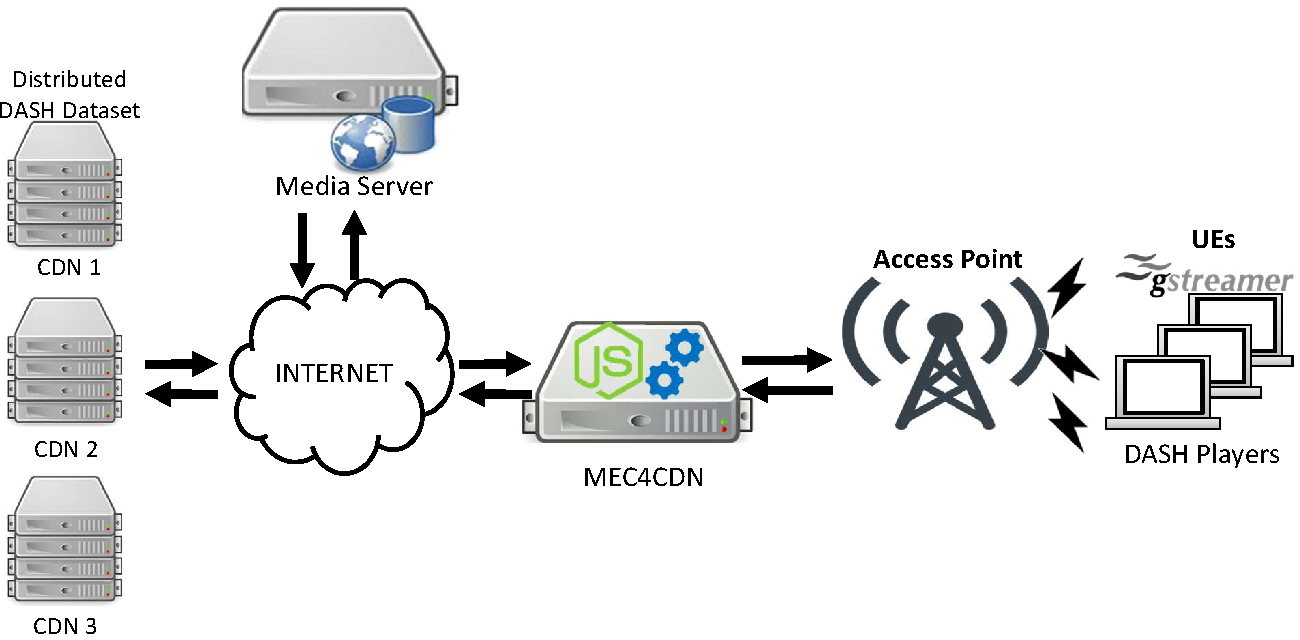
\includegraphics[width=1\textwidth,keepaspectratio]{testbed2.pdf}
	\caption{Testbed.}
	\label{fig:BMSB2018testbed}
\end{figure}

The tests include two different experiments aiming to verify separately the two main features of MEC4CDN:
\begin{itemize}  
	\item Multi-CDN experiment: the proxy server running MEC4CDN employs a multi-CDN infrastructure which allows CDN malfunction detection and switches the content download to an alternative CDN when necessary. In order to simulate CDN malfunctions, we introduce a random latency between 0 and 500 milliseconds on the wired path between the MEC4CDN proxy and the three mirror servers storing the segments.
	\item Local cache experiment: the proxy server running MEC4CDN empowers the content delivery by caching segments at the network edge. This enables the reduction of CDN transactions, while improving the delivery with lower experienced latency.
\end{itemize}

In both experiments, 20 players are sharing both core and network edge resources, competing for the shared wireless access point. The duration of each experiment is fixed to 10 minutes.

Moreover, to get evidence of the benefits of MEC4CDN solution, we carry out the two mentioned experiments where MEC4CDN comes into play and a baseline one without MEC4CDN. This basic setup provides a common delivery infrastructure where the network just forwards the requests to the first CDN. Here, GStreamer players are not able to identify CDN malfunctions, then they use always the same pre-set CDN even when it is suffering severe latency issues. Moreover, no cache is done at the edge, which means that CDN bandwidth is shared among the concurrent clients.


\begin{figure}[htp]
	\centering
	\subfloat[]{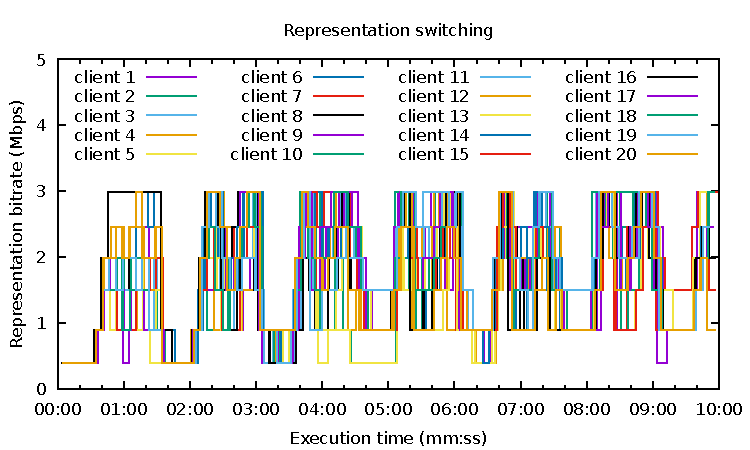
\includegraphics[width=1\textwidth,clip,keepaspectratio]{switch_legacy-cdn.pdf}%
		\label{fig:BMSB2018experiments1c}}
	\hfil
	\subfloat[]{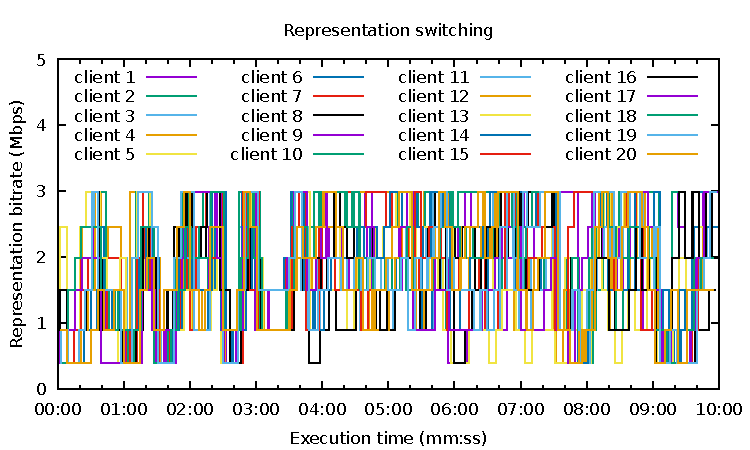
\includegraphics[width=1\textwidth,clip,keepaspectratio]{switch_cdn.pdf}%
		\label{fig:BMSB2018experiments1d}}
	\hfil
	\caption{Representation selection over time: legacy CDN (a) and MEC4CDN multi-CDN (b).}
	\label{fig:BMSB2018experiments1}
\end{figure}

Concerning the first experiment, Figure \ref{fig:BMSB2018experiments1} shows the representation switches along the multi-CDN experiment (10 minutes) where principal CDN suffers performance degradation. In Figure \ref{fig:BMSB2018experiments1c} the actors are not able to take decisions while in Figure \ref{fig:BMSB2018experiments1d} MEC4CDN apply strategies to switch to a healthy CDN. It is clear from the graphs that a legacy solution (\ref{fig:BMSB2018experiments1c}) does not let the players to continue playing at the same representation level when a malfunction occurs while downloading the content. The players reduce the chosen representation bitrate in order to continue playing. In the case of a multi-CDN strategy (\ref{fig:BMSB2018experiments1d}), some players access to higher representation bitrates since the MEC4CDN is able to enforce the delivery by switching to another CDN which better performs.

The improvements are also evident by the eMOS evaluation. The eMOS mean value among all the clients is 3.09 while downloading from a single CDN and 3.47 in case of multi-CDN delivery. This means a eMOS enhancement of +12.3\%.

\begin{figure}[htp]
	\centering
	\subfloat[]{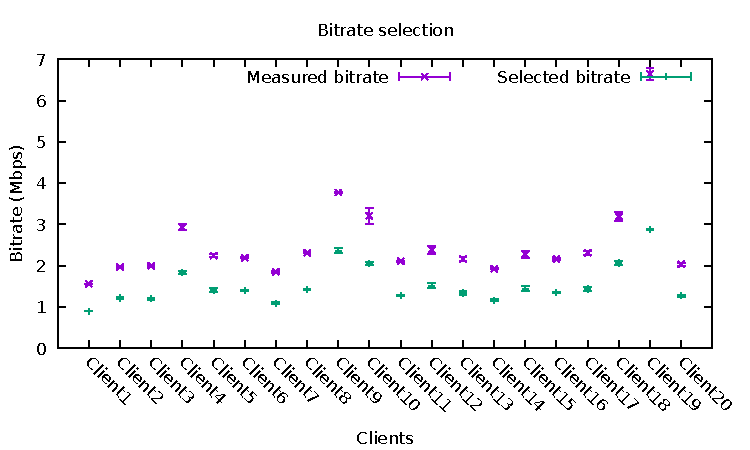
\includegraphics[width=1\textwidth,clip,keepaspectratio]{bitrate_legacy-cache.pdf}
	\label{fig:BMSB2018experiments2a}}
	\hfil
	\subfloat[]{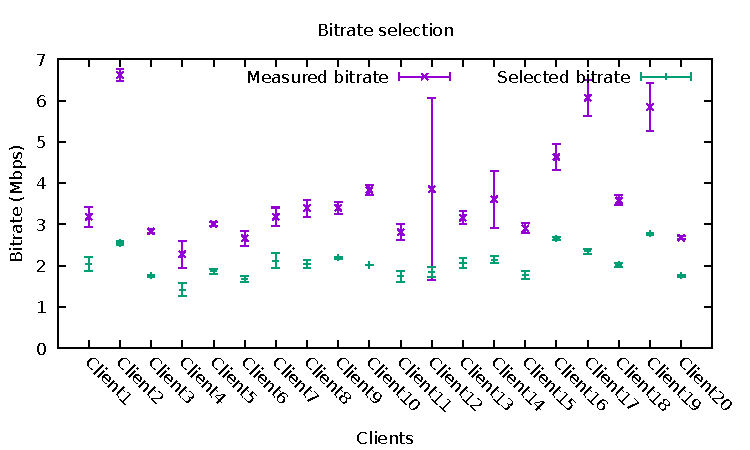
\includegraphics[width=1\textwidth,clip,keepaspectratio]{bitrate_cache.pdf}
	\label{fig:BMSB2018experiments2b}}
	\hfil
	\caption{Mean value and deviation of measured bitrate and selected representation bitrate: legacy content delivery (a) and MEC4CDN cache-powered content delivery (b).}
	\label{fig:BMSB2018experiments2}
\end{figure}

Regarding the second experiment, Figure \ref{fig:BMSB2018experiments2} shows the mean value and the deviation of the measured bitrate and the representation bitrate. The results for a legacy content delivery are shown in Figure \ref{fig:BMSB2018experiments2a} and, when MEC4CDN with local cache delivery is added, the results improve as depicted in Figure \ref{fig:BMSB2018experiments2b}. 
This is clear since the cache lets the player to experience lower latency since the segments are closer to the clients, then the throughput is higher. Therefore, the clients tend to request higher representation bitrate which improves the user's QoE. 

In this case, the eMOS mean value among all the clients is 3.08 in case of legacy delivery and 3.92 in case of cache-powered delivery, which means an eMOS increase of +27.3\%.


\subsection{Conclusion}
\label{sec:BMSB2018conclusion}
This paper proposes a network proxy which enables multi-CDN video distribution and local cache at the network edge by exploiting the MEC architecture proposed by ETSI for future 5G networks.

The proposed proxy has two main outcomes. First, the proxy reduces the CAPEX of the CDN since it makes distributed cache at the network edge, then all the clients can play the contents received from the cache. Second, the proxy shields from CDN malfunction by switching the content download session to another available CDN such to keep QoE rates.

Finally, this proposal has been tested by performing two experiments on a real testbed. The first one exploiting a multi-CDN delivery and the second one employing local cache at network edge. In both the experiments, the results show that the MPEG-DASH players experience higher QoE compared to a legacy content delivery.



%\subsection*{Acknowledgment}

		

%
%%: ----------------------- Related Work ------------------------
% SotA
\part{State of the Art}
\label{sec:Part2}

% this file is called up by thesis.tex
% content in this file will be fed into the main document

%: ----------------------- introduction file header -----------------------


%------------------------------------------------------------------------- 


% the code below specifies where the figures are stored
%\ifpdf
%    \graphicspath{{Content/figures/PNG/}{Content/figures/JPG/}{Content/figures/PDF/}{Content/figures/}}
%\else
%    \graphicspath{{Content/figures/EPS/}{Content/figures/}}
%\fi
\graphicspath{{Content/figures/PNG/}{Content/figures/JPG/}{Content/figures/PDF/}{Content/figures/}{Content/figures/EPS/}}

%Introduction
%\begin{savequote}[50mm]
%If our brains were simple enough for us to understand them, we'd be so simple that we couldn't.
%\qauthor{Ian Stewart }%The Collapse of Chaos: Discovering Simplicity in a Complex World
%\end{savequote}
%[Technologies for interoperable multi-device services]
\chapter{Network-aware content encoding}
\chaptermark{Network-aware content encoding}
\label{chap:network-aware}

\section{Context}

The original uncompressed video content undergoes two main operations before being delivered to the user: compression through one of the widely known video codecs, e.g., H.264 or HEVC, and packaging in a media container format, e.g., MPEG-4 Part 14 (commonly called MP4). Encoding and packaging the content influence user's QoE, which plays a significant role when dealing with media services. Thus, optimizing video encoding and packaging strategy contributes to increase the user's satisfaction and to retain the user from leaving the media service. Considering network information and application context (VOD or real-time communications) may lead to a better selection of video encoding bitrate and streaming format/protocol. In this sense, this thesis investigated the possibility of considering such information by designing and implementing two different solutions that exploit it.

MPEG-DASH natively allows encoding bitrate selection at the client side which enables to mitigate network performance fluctuations. This format also fits with the Video on Demand (VOD) scenario where the latency between content packaging and playback is not an issue. On the contrary, it is not suitable when latency constraints come into play. Live streaming applications, such as video surveillance and video conference, cannot work with typical operational ranges meaning tens of seconds of delay of MPEG-DASH.

In Section \ref{chap:BMSB2020}, an Adaptive Rate Control on top of SRT protocol is developed to demonstrate the applicability of network information at the origin server. Differently from MPEG-DASH, SRT protocol is meant for guaranteeing low latency required for Live streaming, but it does not provide the capability to adapt the encoding bitrate. The implemented Adaptive Rate Control-enabled SRT server periodically changes the video resolution and encoding bitrate to adapt live streams accordingly to the information concerning the network throughput and reported by the connected clients. When network throughput decreases, the resolution and encoding bitrate are decreased to prioritize the playback smoothness over video quality. On the contrary, if the throughput increase, encoding bitrate and resolution are also increased. This solution does not need any additional communication, as SRT protocol already provide feedback mechanisms for reporting network status. Then, this paper proposes a real implementation of an Adaptive Rate Control for SRT streams by including the following relevant contributions:
\begin{itemize}
	\item A server-side Adaptive Rate Control implementation on top of open-source framework for SRT streaming applications. This Adaptive Rate Control exploits the network reports employed by SRT protocol to enable the adaptation of the resolution and encoding bitrate of the content.
	\item A coordinated delivery of the stream as the encoding bitrate is chosen by the origin server at once for all the connected media players. It differs from MPEG-DASH, where each client autonomously choses the representation bitrate.
	\item Evaluation of the effects on user's Quality of Experience (QoE) when compared the proposed solution to a legacy one. In both cases, the player does not need any modification as a legacy SRT client can decode the Adaptive Rate Control-enabled stream.
\end{itemize}
Compared to a legacy SRT solution, the results show that the Adaptive Rate Control-enabled SRT delivery experiences fewer freeze events by enabling switching operations to lower representation bitrates. It reduces the average representation bitrate to prioritize playback smoothness. Moreover, in terms of initial delay, there is not a noticeable difference with legacy SRT since the Adaptive Rate Control does not introduce any delay while starting the streaming session.

Section \ref{chap:BMSB2019} presents a study of LL CMAF to deliver Live Streaming which is carried out to evaluate the trade-off between latency and QoE. CMAF is a technological solution which has two major benefits. First, it pushes MPEG-4 Part 14, usually referred as MP4, as a common file format for different streaming technologies, such as MPEG-DASH or HLS. This feature makes media storage more efficient as different manifests (MPD for MPEG-DASH and M3U8 for HLS) may index the same media segments. Therefore, even if the players download different manifests depending on their supported streaming technologies, they download and play the same media segments. Thus, the remote server (origin server or CDN) needs lower storage capacity. Secondly, it defines a low latency mode, also called chunked mode, named LL CMAF or Chunked CMAF, which enables latency enhancement of the stream, reducing the time elapsed between media packaging and its playback. A typical MPEG-DASH segment contains a single MP4 fragment. On the contrary, LL CMAF enables a single segment to contain multiple fragments. A MP4 fragment is the minimum amount of data required by the player to start decoding the stream. Therefore, the shorter fragment duration allows a promptly playback start, removing the limitation to fully download the entire segment, which usually lasts some seconds. This paper includes:
\begin{itemize}
	\item A server-client solution delivering LL CMAF streams on top of open-source framework. 
	\item A comparison with a legacy MPEG-DASH stream having segments of 2 seconds duration to underline the limitations of the setup widely employed for live/low latency video streaming.
	\item The evaluation of the effects on user's QoE while varying the fragment duration and the resulting latency. The employed fragment durations are 33 ms, 100 ms and 167 ms that correspond to fragments containing a Group of pictures (GOP) with 1, 3 or 5 frames for a video with a nominal framerate of 30 frames per second, respectively.
\end{itemize}
The results show that media players gain lower latency in any of the LL CMAF configurations with respects to legacy MPEG-DASH setup. However, when using an aggressive configuration with a small GOP size and fragment duration, the playback has lower protection against freezes which reduce the QoE. To balance the latency and QoE trade-off, a more conservative configuration of LL CMAF is suggested. 

% !TeX spellcheck = en_US
%Publications.tex
%\newcommand{\PublicationsPath}{PatentsAndPublications/Publications}

%BMSB2020

\section[Adaptive Rate Control for Live streaming using SRT protocol]{Adaptive Rate Control for Live streaming using SRT protocol}
\label{chap:BMSB2020}
\begin{itemize} \itemsep1pt\parskip0pt\parsep0pt
	\item \textbf{Title:} Adaptive Rate Control for Live streaming using SRT protocol
	\item \textbf{Authors:} Roberto Viola, \'Angel Mart\'in, Juan Felipe Mogoll\'on, Alvaro Gabilondo, Javier Morgade and Mikel Zorrilla
	\item \textbf{Proceedings:} 2020 IEEE International Symposium on Broadband Multimedia Systems and Broadcasting (BMSB)
	\item \textbf{Publisher:} IEEE
	\item \textbf{Year:} 2020
	\item \textbf{DOI:}  \url{10.1109/BMSB49480.2020.9379708}
\end{itemize}

\textbf{Abstract:} Media delivery represents one of the main challenges for future networks which aim to converge Broadcast and Broadband video traffic into a common telecommunication network architecture. Nowadays, contents streamed over Internet are delivered in two different manners depending on the application: Video on Demand and Live Streaming. For the former, HTTP-based streaming technologies, such as Dynamic Adaptive Streaming over HTTP (MPEG-DASH), are widely employed for unicast and broadcast communications. It also enables Adaptive Rate Control on the client device allowing players to select a representation and bitrate matching the capabilities of the network at any moment. For the latter, MPEG-DASH does not provide low latency for Live streaming when compared to a Broadcast service. Secure Reliable Transport (SRT) is proposed by SRT Alliance to overcome such limitations of unicast and broadcast communications. Nevertheless, it misses the adaptation of the content to the available network resources. In this paper, we show an implementation of Adaptive Rate Control for SRT protocol which exploits periodical network reports in order to adapt the content encoding process. The evaluation includes a real deployment of the solution and a comparison with a legacy SRT stream.

\textbf{Keywords:} Rate Control, Traffic and performance monitoring, Secure Reliable Transport, Video coding and processing.

\subsection{Introduction}
MPEG-DASH \cite{sodagar2011mpeg} and other HTTP-based alternatives are widely employed solutions for media services. It is compatible with existing HTTP-based Internet infrastructure and allow resolution and encoding bitrate selection to mitigate network performance fluctuations in unmanned networks. These solutions perfectly fit for Video on Demand (VOD) scenario where the latency between content packaging and playback is not an issue. On the contrary, they are not suitable when latency constraints come into play. Live streaming applications, such as video surveillance and video conference, cannot work with tens of seconds of delay of HTTP-based solutions.

Real Time Streaming Protocol (RTSP) and Real Time Messaging Protocol (RTMP) are legacy protocols for Real-time streaming which enable lower latency than HTTP-based solutions. Nevertheless, they are designed to work in unicast mode, meaning that the communication is based on a server-client delivery where the server sends the content in push mode. This communication model fails when players scale up to broadcast concurrency rates, since the server should push as many unicast steams as the number of connected players. Moreover, these solutions suffer of network restrictions applied by network functions, such as firewall and NAT, blocking the delivery of those streams.

Secure Reliable Transport (SRT) protocol \cite{srt2018} is the proposal of SRT Alliance to fill this gap. It lets to gain scalability of Broadcast delivery while guaranteeing low latency required for Live streaming. SRT has been designed to work in both push and pull mode, then allows to stream content even when firewalls and NATs network functions are present. The protocol also includes forward error correction (FEC) \cite{luby2002} which enforces resilience from transmission errors. SRT server also employs network reports from the client to adapt packet overhead. Thus, the server upload speed depends on network throughput and packets are not lost when the available throughput is enough to send the content to the client. Lost packets are re-transmitted only if the network throughput can absorb such overhead.

SRT does not interfere with content encoding, then network reports are never exploited to adapt resolution and encoding bitrate of the content as it happens in HTTP-based solutions. Enabling content adaptation on top of SRT allows two main advantages. First, in case of network degradation, it shields from playback stalls by reducing the bitrate of the content to be send, as MPEG-DASH does. Second, it allows to send a representation matching the client display features. This work proposes a real implementation of an Adaptive Rate Control for SRT streams. This solution includes two relevant contributions:
\begin{itemize}
	\item A server-side Adaptive Rate Control implementation on top of Open Source framework for SRT streaming applications. This Adaptive Rate Control exploits the network reports employed by SRT protocol to enable the adaptation of the resolution and encoding bitrate of the content.
	\item Evaluation of the effects on user's Quality of Experience (QoE) when compared the proposed solution to a legacy one.
\end{itemize}

The rest of this paper is organized as follows. First, section \ref{sec:BMSB2020related} presents the background of Video Streaming solutions and performance metrics. Then, section \ref{sec:BMSB2020implementation} shows the implementation of our Adaptive Rate Control on top of SRT streams. In section \ref{sec:BMSB2020results} we describe the experiments and present the results. Finally, in section \ref{sec:BMSB2020conlusion} we expose the conclusions and future work.


\subsection{Related Work}
\label{sec:BMSB2020related}

\subsubsection{Overview of Video Streaming}
\label{sec:BMSB2020streaming}

MPEG-DASH \cite{sodagar2011mpeg} was developed by MPEG and standardized by ISO/IEC. MPEG-DASH is a pull-based streaming technology over HTTP, where the client requests the content from a conventional HTTP server which stores it split into segments and encoded at many representation levels. A segment consists in a unique ISO Base Media File Format fragment, usually called MP4 fragment, which is the minimum playable data. First, the client fetches a manifest file, referred as Media Presentation Description (MPD), and parses it to be aware of the different representations of the content. Then, the client downloads the segments corresponding to the representation that matches the device capabilities and user preferences in terms of resolution, language, codec and bitrate. Each time the client requests the next segment, it can switch to a different representation depending on network performance to avoid playback degradation and maximize user's QoE. Thus, the Adaptive Rate Control is fully managed by the client during the streaming session. However, the delay of MPEG-DASH streams is high since, by design, it is not possible to go behind the segment duration, which usually ranges from 2 to 30 seconds. Thus, MPEG-DASH is not suitable for real-time applications. Apple HTTP Live Streaming (HLS) and Microsoft Smooth Streaming are other solutions working with a similar workflow to MPEG-DASH, where the format of the manifest file differs, and experience delays with the same order of magnitude.

The Common Media Application Format (CMAF) \cite{hughes2017information}, proposed by ISO/IEC, tries to overcome such latency limitations of MPEG-DASH by introducing a Low Latency mode, namely Low Latency or Chunked CMAF. Chunked CMAF allows the presence of several MP4 fragments inside one segment. Consequently, the buffering done by the client is shorter as it can start to play the content even if the segment is not completely downloaded, it just needs to have a MP4 fragment. In \cite{wei2014} and \cite{essaili2018}, two different implementations of Chunked CMAF are presented. The former, \cite{wei2014} still evidences latency in the order of 1 second, the latter, \cite{essaili2018} reduces latency behind one second by generating fragments containing just one frame. The use of just one frame introduces a heavy overhead inside the communication since MP4 header must be replicated each time a fragment is sent. Moreover, it comes at cost of reduced QoE since smaller fragments causes a smaller playout buffer which more easily can go empty \cite{viola2019}. Nevertheless, Chunked CMAF is not currently used by the media industry, but it is a promising solution for the future.

In any case, HTTP-based solutions were not designed for real time applications. Thus, achieving similar latency performance as real-time designed protocols, based on Real-time Transport Protocol (RTP) and User Datagram Protocol (UDP) \cite{schulzrinne1996rtp}, is complicated.
RTP Control Protocol (RTCP) \cite{ott2010} was designed to work jointly with RTP. Hence, RTCP does not transfer streaming data, but it provides RTP with an out of band channel to get feedback on the network statistics, enabling RTP to control the transferring rate. However, such adaptation is made at the network interface level. Then, it does not imply changes on the bitrate of the encoder that could make the difference to adapt the throughput to the available network bandwidth, preventing packet losses. RTP-based solution has also some drawbacks. On the one hand, RTCP is designed to work with unicast streams and, on the other, RTCP is only compatible to push communications mode. Thus, it is difficult to scale as the number of clients increases and when firewalls and NATs are present.

Periscope, one of the most common live streaming services, overcomes these issues by using a hybrid RTMP and HLS solution \cite{wang2016anatomy}. Here, the streaming protocol is chosen depending on the volume of clients and latency trade-off. For streaming sessions involving few clients, RTMP is preferred to reduce latency. When the number of clients increases, HLS is exploited to reduce overheads at the server.

SRT \cite{srt2018} protocol, proposed by SRT Alliance, is the media industry solution to transfer live broadcast streaming under the constraint of low latency. The protocol also includes a mandatory encryption to enforce the security. SRT allows both push and pull modes which means that, in case of network traversal barriers, pull mode could bridge them. Moreover, the use of a FEC mechanism \cite{luby2002} enforces resilient communication. Network feedback reports are also exploited to tune the packet overhead and provide protection against transmission errors. In case of packet losses, they are re-transmitted or discarded depending on the configured maximum latency and on the network possibilities to support such overhead.

Finally, SRT includes many advantages compared to conventional real time protocols, but it still lacks the capability to adapt the bitrate throughput of the content when the network bandwidth changes. Network reports are exploited to tune the transferring rate, but they are not accessible by the encoding process. Consequently, resolution and encoding bitrate of the content are neither adapted at the server nor at the client as it happens in HTTP-based solutions.

\subsubsection{Performance metrics}
\label{sec:BMSB2020realtime}

All the proposed streaming technologies have a common aspect, they need to focus not only on reducing the latency to allow live streaming, but also on maximising the QoE to retain user when satisfying expectations. The QoE is a key aspect for user satisfaction and retention when rating streaming services. An exhaustive QoE evaluation requires a demographic perception study to get a Mean Opinion Score (MOS) \cite{Itu2016}.

Nevertheless, there are many studies in literature which demonstrate that the use of objective performance metrics is helpful to provide an estimation of user's QoE \cite{Alreshoodi2013}.

In \cite{claeys2014} the authors consider stalling time, number of representation switches and inter-switching time as objective metrics to estimate user's QoE. Recently, the work \cite{lentisco2017} also includes initial buffering.
In both cases, the proposed performance metrics are applicable only for HTTP-based streaming applications involving content adaptation. Since our solution aims to include the same feature on top of SRT protocol, the same performance metrics can be assessed.

\subsection{Adaptive Rate Control Implementation}
\label{sec:BMSB2020implementation}

\begin{figure}[htp]
	\centering
	
\includegraphics[width=1\textwidth,keepaspectratio]{scenario.pdf}
	\caption{System architecture for SRT streaming.}
	\label{fig:BMSB2020system}
\end{figure}

The system architecture for delivering SRT streams is depicted in Figure \ref{fig:BMSB2020system}. The system is composed by a Live Source, a SRT Media Server and a SRT Player.

The Live Source is the node which provides the content to the processing and delivery pipeline. Here, many different entities can act as a Live source, e.g. a camera or a video software editor.

The SRT Media Server processes the content ingested by the Live Source and delivers it to the SRT Player after encoding and packetizing it into an SRT-compliant stream. Thus, it accomplishes the following tasks:
\begin{itemize}
	\item Encoding: it encodes the content into a live H.264 bitstream \cite{wiegand2003}. In a legacy SRT solution, the video frame resolution and encoding bitrate is chosen when launching the encoding process and kept unaltered during all the process. In our approach, both resolution and bitrate can be dynamically changed during the streaming session to provide different representation levels of the same content.
	\item Muxing: H.264 bitstream is packetized into a MPEG-2 Transport Stream (MPEG-TS) container \cite{sarginson1996}.
	\item Encryption: MPEG-TS is encrypted though 128/256 bit Advanced Encryption Standard (AES) \cite{chown2002advanced}. This is a mandatory feature included in SRT to enforce end-to-end security.
	\item Delivery: SRT employs User Datagram Protocol (UDP) to transmit data over the network to the client since it guarantees lower latency than Transmission Control Protocol (TCP), which is commonly used by HTTP-based streaming solutions. However, UDP is not reliable since it does not provide mechanisms to compensate for transmission errors. Then, SRT includes Forward Error Correction (FEC) and re-transmission mechanisms on top of UDP delivery to allow the SRT Player to recover from lost or corrupted packets.
	\item Monitoring: SRT server receives network reports from the SRT Player which contain information related to network status (bandwidth and delay) and packet transmission (sent, lost or re-transmitted packets number). In a legacy SRT solution, reports are only employed to tune the sending transmission rate and schedule the transmission of new and/or lost packets. In our approach, network reports are also captured and employed to select the appropriate representation level (resolution and bitrate) to be used by the encoding process.
\end{itemize}

We employ GStreamer \cite{gstreamer} in its v1.14 stable release to develop our Adaptive Rate Control-enabled SRT Media server. We select and setup the following plugins to accomplish the above tasks:

\begin{itemize}
	\item \textit{H.264 encoder}: the setup of the encoder is key to allow the adaptation of the representation (resolution and bitrate) of the content according to the measured network statistics. \textit{Keyframes} (I-frames) do not require any other frames to be decoded, so the player can always start decoding a stream from a \textit{keyframe}. Thus, \textit{keyframes} are essential for live streaming to start playing the content as soon as possible when the player starts receiving the content. Moreover, in our Adaptive Rate Control-enabled stream, when it switches the representation level, it introduces a discontinuity. Thus, it makes new frames, with a different resolution and encoding bitrate, not possible to be decoded based on the previous frames. The player needs a new \textit{keyframe} to decode the stream every time the representation level changes. Then, the Adaptive Rate Control forces the encoder to introduce a \textit{keyframe} every time a representation switch is performed.
	\item \textit{MPEG-TS muxer}: it packetizes H.264 encoded frames into MPEG-TS chunks. Each chunk cannot contain data at different representation levels. Then, it is mandatory that each MPEG-TS chunk starts with a \textit{keyframe}.
	\item \textit{SRT server sink}: it receives MPEG-TS chunks from the muxer, it encrypts and encapsulates them into UDP packets before sending them to the player. This plugin gets active, sending packets, only when a client is connected.
	It also monitors the network by getting network statistics measured during the transmission of the video stream to the client. A legacy SRT server sink uses statistics only to adapt the network overhead of the transmission, to reduce packets lost and to avoid re-transmissions. Additionally, the proposed Adaptive Rate Control-enabled solution exploits this information to dynamically change the setup of the encoder plugin to switch to a suitable representation level.
\end{itemize}

Finally, SRT player is implemented with GStreamer release (v1.14) \cite{gstreamer}. This version provides SRT client and decoding capabilities. Thus, it can play SRT legacy streams. Moreover, the aggregation of the Adaptive Rate Control to the SRT Media server does not cause any relevant change in the protocol. This means that developing a custom client application is not required and the generated SRT stream can be played by any SRT-compliant player.

\begin{figure}[htp]
	\centering 
	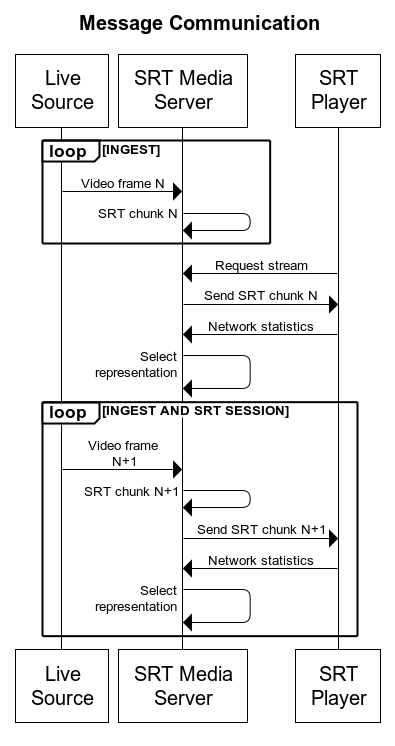
\includegraphics[width=0.6\textwidth,keepaspectratio]{webseq.png}
	\caption{Sequence diagram.}
	\label{fig:BMSB2020sequence}
\end{figure}

The communication between the systems in the setup is shown in Figure \ref{fig:BMSB2020sequence}. SRT Media Server starts to encode and packetize video frames when the Live Source is connected. Video frames are H.264 encoded and MPEG-TS muxed, then packetized into SRT chunks.
Nevertheless, data are not transmitted until an SRT player connects to the SRT Media Server. It means that chunks can be discarded by the server if there are no players. The SRT Media Server only stores the most recent chunks with a buffer size of "maximum allowed latency". This operation is necessary in order to guarantee that only the most recent chunks are sent, then achieve a low latency live streaming. In GStreamer, maximum allowed latency is configurable, but we decide to keep it to its default value which is 125 ms. Once the SRT player is connected, SRT Media Server starts delivering the content to the player. While receiving the content, the SRT player stores it in the playback buffer before decoding and displaying it. The playback buffer is set to 1 seconds to balance low latency, packet losses reliability and changeable network conditions.

To adapt the representation, the implemented Adaptive Rate Control accesses network statistics from the SRT server sink plugin and exploits the information to tune the configuration of the H.264 encoder. This evaluation is performed by the Adaptive Rate Control once per second. The decision algorithm of the implemented Adaptive Rate Control is shown in Algorithm \ref{alg:BMSB2020algorithm}. The algorithm takes the last measured network bandwidth (\textit{bw$_t$}), round-trip delay time (\textit{rtt$_t$}) and send rate (\textit{rate$_t$}) from SRT network reports, the current employed representation level (\textit{rep$_t$}) and the list of all the available ones (\textit{\{rep$_{list}$\}}). Bandwidth and round-trip delay time are employed to evaluate the maximum allowed network throughput (\textit{throughput$_{max_t}$}) through the Equation \ref{eq:BMSB2020thoughput}.

\begin{algorithm}
	\renewcommand{\algorithmicrequire}{\textbf{Input:}}
	\renewcommand{\algorithmicensure}{\textbf{Output:}}
	\caption{Adaptive Rate Control}
	\label{alg:BMSB2020algorithm}
	\begin{algorithmic}
		\Function{adaptiveRate}{bw$_{t}$, rtt$_{t}$, rate$_{t}$, rep$_{t}$, $\{rep_{list}\}$}
		\Require bw$_t$ \Comment{measured bandwidth}
		\Require rtt$_t$ \Comment{measured delay}
		\Require rate$_t$ \Comment{measured send rate}
		\Require rep$_t$ \Comment{current representation}
		\Require $\{rep_{list}\}$ \Comment{available representations}
		\Ensure rep$_{t+1}$ \Comment{next representation}
		\State throughput$_{max_t}$ $\leftarrow$ bw$_{t}$, rtt$_{t}$ \Comment{network throughput}
		\ForAll { rep$^{i}$ $\in$ $\{rep_{list}\}$ } \Comment{for each representation}
		\State bitrate$^{i}_{t}$ $\leftarrow$ rep$^{i}$, rate$_{t}$, rep$_t$ \Comment{\parbox[t]{0.31\linewidth}{minimum network bitrate}}
		\If {(throughput$_{max_t}$ $>$ throughput$^{i}_{t}$)} %\Comment{\parbox[t]{0.1\linewidth}{network admits the bitrate}}
		\State \Comment{network admits the representation}
		\State rep$_{t+1}$ $\leftarrow$ rep$^i$ \Comment{next representation}
		\EndIf
		\EndFor
		\EndFunction
	\end{algorithmic}
\end{algorithm}

\begin{equation}
\label{eq:BMSB2020thoughput}
throughput_{max_t} = bw_t * \frac{1}{1 + \frac{rtt_t}{2}}
\end{equation}

Then, for each available representation, the required network throughput to allow its transmission is calculated. It is important to note that each representation means a different throughput configured by the encoding bitrate. Furthermore, the encoding bitrate needs to accommodate a gap to allow that protocols messages and extra information from other levels of the ISO/OSI model, added to the encoded video payloads, still meet network bandwidth thresholds.

Consequently, to establish if it is possible to stream a specific representation to the client, we should compare the maximum allowed network throughput (\textit{throughput$_{max_t}$}) with the throughput that the representation would generate (\textit{throughput$^i_t$}). Since we cannot access the employed throughput before streaming the content, we estimate it from the current send rate (\textit{rate$_t$}) provided by the network reports. Equation \ref{eq:BMSB2020minBW} estimates the necessary network throughput (\textit{throughput$_t^i$}) to allow the representation (\textit{rep$^i$}) bitrate to be streamed. The ratio between current send rate (\textit{rate$_t$}) and current representation encoding bitrate (\textit{rep$_t$}) is the current overhead, then we multiply it per the representation encoding bitrate (\textit{rep$^i$}).

\begin{equation}
\label{eq:BMSB2020minBW}
%bitrate^{i}_{t} = rep^i * \frac{rate_{t}}{rep_{t}}
throughput^{i}_{t} = rep^i * \frac{rate_{t}}{rep_{t}}
\end{equation}

If the estimated throughput (\textit{throughput$_t^i$}) is lower than the maximum allowed throughput (\textit{throughput$_{max_t}$}), it means that the representation can be sent. The output of the algorithm is the selected representation to be employed at the H.264 encoder. The encoder is configured to immediately generate a \textit{keyframe} and switch at the new selected representation resolution and encoding bitrate.

\subsection{Results}
\label{sec:BMSB2020results}

The experimental setup employed for testing the implemented Adaptive Rate Control is presented in Figure \ref{fig:BMSB2020setup}. The overall setup comprises the following nodes:
\begin{itemize}
	\item STR Media Server and Traffic Control: this is a unique physical node which embeds two logical systems. We employ a Docker containerization \cite{merkel2014} to run different functions in separated environments. A Docker container running Ubuntu 19.04 OS includes the Adaptive Rate Control-enabled SRT Media Server developed through GStreamer framework \cite{gstreamer}. The container communicates with the host machine running Ubuntu 16.04 OS which forwards data to the physical network interface. On the host machine, we periodically modify bandwidth and latency of the network interface. Traffic Control \cite{tc} is the utility to change the uplink capacity. To emulate an LTE network, we use the \textit{European Broadband user experience} dataset collected and publicly provided by the Joint Research Centre (JCR) of the European Commission \cite{chawdhry2016}. The dataset provides both bandwidth and latency that we apply through Traffic Control utility. The interval between two consecutive network changes is set to 100 ms. %, aligned with the dataset sample rate.
	\item Network switch: this node provides wired network access to both server and player nodes to communicate each other. It forwards all the incoming traffic on both sides.
	\item SRT Player: this node run a GStreamer application to receive the SRT stream and play it.
\end{itemize}

\begin{figure}[htp]
	\centering
	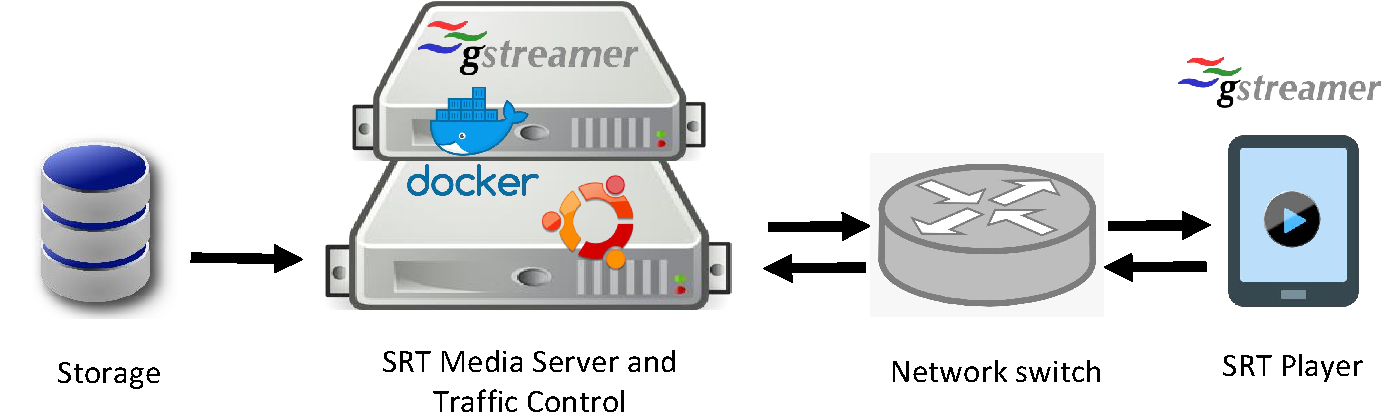
\includegraphics[width=1\textwidth,keepaspectratio]{testbed.pdf}
	\caption{Experimental setup.}
	\label{fig:BMSB2020setup}
\end{figure}

\begin{table}[htp]
	\caption{Set of representations employed in the experiments.}
	\centering
	\bgroup
	\def\arraystretch{1.2}%  1 is the default, change whatever you need
	\setlength\tabcolsep{2.5pt} % default value: 6pt
	\label{tab:BMSB2020reps}
	{\scriptsize
		\begin{tabular}{>{\centering\arraybackslash}m{\dimexpr0.1\textwidth-2\tabcolsep-\arrayrulewidth\relax}
				>{\centering\arraybackslash}m{\dimexpr0.15\textwidth-2\tabcolsep-\arrayrulewidth\relax}
				>{\centering\arraybackslash}m{\dimexpr0.15\textwidth-2\tabcolsep-\arrayrulewidth\relax}
				>{\centering\arraybackslash}m{\dimexpr0.15\textwidth-2\tabcolsep-\arrayrulewidth\relax}
			}
			\toprule
			\textbf{Index} & \textbf{bitrate (kbps)} & \textbf{resolution} & \textbf{framerate (FPS)} \\
			\midrule
			\midrule
			1 & 1200 & 640x360 & 24 \\
			2 & 2250 & 1280x720 & 24 \\
			3 & 4500 & 1920x1080 & 24 \\
			\bottomrule
			\bottomrule
		\end{tabular}
		\egroup
	}
\end{table}

We perform different experiments to compare the Adaptive Rate Control-enable SRT stream with a legacy SRT stream. We use a locally stored Big Buck Bunny test sequence to feed the SRT Media Server. Its raw version is provided by Xiph.Org Foundation \cite{xiph}. For the Adaptive Rate Control-enabled stream, we established three different representation levels to be employed by the H.264 encoder, while legacy one employs only the higher one. The representations are shown in Table \ref{tab:BMSB2020reps}.

The duration of each SRT streaming session lasts 594 seconds which is the duration of the employed test sequence. The results of the two strategies in terms of representation switches, freezes, initial delay and average representation bitrate are shown in Table \ref{tab:BMSB2020results}.

\begin{table}[htp]
	\caption{Number of switches (\textit{S$_{Nb}$}), number of freezes (\textit{F$_{Nb}$}), average freeze duration (\textit{F$_{avg}$}), initial delay (\textit{D}) and average representation bitrate (\textit{R$_{avg}$}) for both legacy and Adaptive Rate Control-enabled SRT streams.}
	\centering
	\def\arraystretch{1.2}%  1 is the default, change whatever you need
	\setlength\tabcolsep{2.5pt} % default value: 6pt
	\label{tab:BMSB2020results}
	{\scriptsize
		\begin{tabular}{>{\centering\arraybackslash}m{\dimexpr0.2\textwidth-2\tabcolsep-\arrayrulewidth\relax}
			>{\centering\arraybackslash}m{\dimexpr0.1\textwidth-2\tabcolsep-\arrayrulewidth\relax}
			>{\centering\arraybackslash}m{\dimexpr0.1\textwidth-2\tabcolsep-\arrayrulewidth\relax}
			>{\centering\arraybackslash}m{\dimexpr0.1\textwidth-2\tabcolsep-\arrayrulewidth\relax}
			>{\centering\arraybackslash}m{\dimexpr0.1\textwidth-2\tabcolsep-\arrayrulewidth\relax}
			>{\centering\arraybackslash}m{\dimexpr0.1\textwidth-2\tabcolsep-\arrayrulewidth\relax}
		}
		\toprule
		\textbf{SRT server} & \textbf{S$_{\textbf{Nb}}$} & \textbf{F$_{\textbf{Nb}}$} & \textbf{F$_{\textbf{avg}}$(ms)} & \textbf{D(ms)} & \textbf{R$_{\textbf{avg}}$(kbps)}\\
		\midrule
		\midrule
		Legacy & 0 & 122 & 820 & 972 & 4500 \\
		Adaptive Rate Control & 197 & 87 & 727 & 986 & 4028 \\
		\bottomrule
		\bottomrule
	\end{tabular}
	}
\end{table}

\begin{figure}[htp]
	\centering 
	\includegraphics[width=1\textwidth,keepaspectratio]{reps.eps}
	\caption{Representation bitrate selection.}
	\label{fig:BMSB2020selection}
\end{figure}

In terms of switches, Adaptive Rate Control solution performs 197 representation switches, while it is not applicable to the legacy SRT stream. Figure \ref{fig:BMSB2020selection} shows the distribution of the switches across the streaming session. Legacy stream is stable to 4500 kbps encoding bitrate, while seems that Adaptive Rate Control one never uses the lowest encoding bitrate (1200 kbps) but moves between the other two (4500 and 2250 kbps). Thus, it causes that the average representation bitrate is 10\% lower when using the Adaptive Rate Control (4028 kbps against 4500 kbps). In terms of initial delay, there is not a noticeable difference since the Adaptive Rate Control does not introduce any delay while starting the streaming session. On the contrary, our Adaptive Rate Control solution outperforms legacy one while considering number of freezes and their duration. Here, the proposed solution scores 29\% less freezes events, and their average duration is 11\% shorter.

These results show that our solution sacrifices average representation bitrate in order to reduce freezes events. Fewer freezes events lead to a smoother video playback for the end user.

\subsection{Conclusions and Future Work}
\label{sec:BMSB2020conlusion}
This paper proposes an Adaptive Rate Control for SRT protocol to deliver live streaming content, while coping with transmission variability due to network degradation or issues.

The proposed solution is integrated with Open Source GStreamer multimedia framework and tested by altering the network capabilities according to real LTE measurements provided by a publicly available dataset.

Compared to a legacy SRT solution, the results show that Adaptive Rate Control-enabled SRT delivery experiences fewer freeze events by enabling switching operations to lower representation bitrates. Thus, it reduces the average representation bitrate to prioritize playback smoothness.


% use section* for acknowledgement
%\subsection*{Acknowledgment}
% !TeX spellcheck = en_US
%Publications.tex
\newcommand{\PublicationsPath}{PatentsAndPublications/Publications}

%BMSB2019

\section[QoE-based enhancements of Chunked CMAF over low latency video streams]{QoE-based enhancements of Chunked CMAF over low latency video streams}
\label{chap:BMSB2019}
\begin{itemize} \itemsep1pt\parskip0pt\parsep0pt
	\item \textbf{Title:} QoE-based enhancements of Chunked CMAF over low latency video streams
	\item \textbf{Authors:} Roberto Viola, Alvaro Gabilondo, \'Angel Mart\'in, Juan Felipe Mogoll\'on and Mikel Zorrilla
	\item \textbf{Proceedings:} 2019 IEEE International Symposium on Broadband Multimedia Systems and Broadcasting (BMSB)
 	\item \textbf{Publisher:} IEEE
	\item \textbf{Year:} 2019
	\item \textbf{DOI:}  \url{10.1109/BMSB47279.2019.8971894}
\end{itemize}	

\textbf{Abstract:} 5G infrastructures are in the roadmap of content delivery services, aiming to forward all broadcast and broadband video traffic using a common telecommunication network architecture. Streaming services will benefit from 5G networks which promise higher capacity, higher bandwidth and lower latency than current infrastructures. However, the widely employed streaming technologies, such as Dynamic Adaptive Streaming over HTTP (MPEG-DASH), require an intrinsic high latency of tens of seconds to enforce the Quality of Experience (QoE). These conditions turn MPEG-DASH unfavourable when compared with a traditional broadcast pipeline for live events in terms of latency. Therefore, improvements on latency of streaming technologies are necessary to deliver live broadcast services over 5G networks. The media industry proposed a Chunked Common Media Application Format (Chunked CMAF) in order to achieve latency under a second. In this paper, we show an implementation of a Chunked CMAF for MPEG-DASH live videos in a real deployment. To further evaluate the benefits of CMAF we evaluate the QoE results when delivering a legacy MPEG-DASH live content compared to a Chunked CMAF-powered one.

\textbf{Keywords:} Chunked CMAF, Future broadcasting services, MPEG-DASH, Quality of Experience, Video coding and processing.

\subsection{Introduction}
% no \IEEEPARstart
Video streaming services represent a large fraction of the Internet traffic. In fact, live video traffic will grow 3-fold from 2017 to 2022, accounting the 17\% of all internet video traffic \cite{ciscovideo2017}. This trend would be fuelled by the deployment of 5G networks, which will enable the cooperation between broadband and broadcast services \cite{calabuig2015}.

5G networks promise high capacity, high bandwidth and low latency to cope with demanding traffic and services. Nevertheless, MPEG-DASH and other HTTP-based alternatives require to packetize video contents in segments with a duration in the order of seconds to enforce the QoE, leading to tens of seconds of delay between content generation and consumption \cite{lohmar2011}. This delay is produced by the duration of packaged media segments, designed to match changeable network delivery performance, and the required buffering, done by the media player to achieve a smooth playback for \mbox{on-demand} and live streams. This delay is not significant for \mbox{on-demand} contents, but it is too high to deliver live streams with comparable performance to the broadcast live services. Moreover, when deploying hybrid broadcast broadband services, the common mechanism to synchronize broadcast and broadband signals consists in delaying the broadcast source as broadband stream is usually 30-40 seconds delayed with respect to the broadcast service.

The Common Media Application Format (CMAF) \cite{hughes2017information}, proposed by ISO/IEC, is the solution for delivering live contents from media industry. CMAF includes two major benefits. First, it ensures the use of the ISO Base Media File Format, usually referred as MP4, as a common file format when combined with different streaming technologies such as MPEG-DASH or HTTP Live Streaming (HLS). This feature makes media storage more efficient as different manifests (MPD for MPEG-DASH and M3U8 for HLS) may index the same segments. Each media client can download a different manifest depending on its supported streaming technologies. Then, it plays the content by downloading the same media segments. Thus, the server needs lower storage capacity. Secondly, it defines a chunked mode, named Chunked CMAF or Low Latency CMAF, which enables latency enhancement of the stream, reducing the time elapsed between media packaging and its playback.

\begin{figure}[htp]
	\centering
	\includegraphics[width=1\textwidth,keepaspectratio]{CMAF.eps}
	\caption{Legacy fragment and Chunked CMAF fragment.}
	\label{fig:BMSB2019fragment}
\end{figure}

Typical MPEG-DASH media segments contain a single MP4 fragment with the fragment duration equal to the segment duration. Here, common values for segment duration are from 2 to 30 seconds. On the contrary, Chunked CMAF enables a single segment to contain multiple fragments as depicted in Figure \ref{fig:BMSB2019fragment}. Therefore, Chunked CMAF exploits the use of short MP4 fragments, including the minimum data required by the player to start decoding the stream. Therefore, the shorter fragment duration allows a promptly playback start, removing the limitation to fully download the entire segment. 

This work proposes a real implementation of a server-client solution delivering Chunked CMAF streams of live contents. This solution has been achieved by providing two relevant contributions:
\begin{itemize}
	\item Chunked CMAF has been integrated with an Open Source MPEG-DASH framework.
	\item The evaluation measures the effects on user's QoE while varying the fragment duration of the Chucked CMAF segments and the resulting latency.
\end{itemize}

The remainder of this paper is organized as follows. First, section \ref{sec:BMSB2019related} presents the background of the MPEG-DASH standard and Chunked CMAF for deploying live media services. Then, section \ref{sec:BMSB2019implementation} shows the implementation of Chunked CMAF solution. In section \ref{sec:BMSB2019results} we describe the experiments and present the results. Finally, in section \ref{sec:BMSB2019conlusion} we expose the conclusions and future work.

\subsection{Related Work}
\label{sec:BMSB2019related}
In this section, it is included an overview of MPEG-DASH for live streaming services and afterwards, a comprehensive review about the State of Art of Chunked CMAF is described.

\subsubsection{Overview of Live MPEG-DASH}
\label{sec:BMSB2019dash}
MPEG-DASH was developed by MPEG and standardized by ISO/IEC. In MPEG-DASH, first, the client fetches a Media Presentation Description (MPD) and parses it to be aware of the different representations of the content. Then, the player chooses the representation that fits in the device capabilities in terms of resolution, language, codec and bitrate. Accordingly, the client requests and downloads the corresponding segment from the server. Once a segment has been played, the next one from the MPD is requested. During the playback, the player can switch to a different representation depending on its preferences and network performance in order to minimize any impact on the QoE.

The live playback is possible through the \textit{availabilityStartTime} field in the MPD, which marks the UTC time when the stream is made available. The client continuously compares it with the current time to fetch the last available segments. In the case of a legacy live MPEG-DASH content, the \textit{availabilityStartTime} has to correspond to the time when the first media segment is fully available on server side. Then, the segment duration, which ranges from 2 to 30 seconds, is the minimum delay that a client experiences during a live stream. Encoding and network latency also influence this delay, but their weights in the resulting latency are 10-100ms when aggregated to the segment duration.

\subsubsection{Chunked CMAF}
\label{sec:BMSB2019cmaf}
The latency is a key factor when dealing with live streaming contents. Current MPEG-DASH-based solutions are not able to operate with a similar latency to the current broadcast solutions. This is a major challenge when targeting broadcast levels of QoE. The use of Chunked CMAF, together with improved network bandwidth and latency of the 5G networks, aims to reduce live streaming latency and keep it behind a second \cite{bouzakaria2014overhead}.

Contrary to the legacy MPEG-DASH streams, a Chunked CMAF-compliant MPEG-DASH distinguishes between MP4 fragment duration and media segment duration with different values. The reduction of the fragment duration makes the media units of the stream quickly available enabling prompt playback. Consequently, the segment contains multiple fragments and the \textit{availabilityStartTime} attribute contained in the MPD must be set at the time the first fragment is available, even if the segment is not completely written. The smaller the fragment is, the smaller delay is experienced by the player. Theoretically, fragment duration can be reduced to one frame duration. To this end, it is required a proper server, which must be able to split the HTTP response sending fragment units instead of the full segment.

Several implementations serve Chunked CMAF with \mbox{HTTP 1.1} Chunked Transfer Encoding. The server encapsulates each MP4 fragment in a HTTP chunk and deliver it over time, instead of sending the entire segment at once. In \cite{saminathan2011}, Chunked Transfer Encoding allows a \mbox{HTTP 1.1} server to split the response in small HTTP chunks. The paper shows that the latency does not depend on the segment duration but depends on the duration chosen for the HTTP chunks. This approach still uses one second duration chunks while splitting the HTTP connection between server and player. The author of \cite{essaili2018} also implements a MPEG-DASH delivery involving Chunked CMAF, but it varies the duration of the fragment. Both papers provide performance results in terms of overall latency.

The work shown in \cite{wei2014} uses HTTP 2.0 to exploit the \mbox{push-mode} added in the new HTTP version for reducing the latency. HTTP 2.0 does not have a Chunked Transfer \mbox{Encoding} mode, since it already employs a frame-based \mbox{delivery}, i.e. it splits the response in several frames which contain the Chunked CMAF MP4 fragments. This solution has the \mbox{advantage} of reducing the protocol header overhead since HTTP 2.0 header is simplified when compared to HTTP 1.1. However, push-mode reduces the adaptation possibilities at the client-side to dynamically select an appropriate representation for the network performance conditions. Decisions can be still done by the server, modifying the MPD, but this approach does not scale as the player-side decisions when working in pull-mode.

\subsubsection{QoE Metrics}

The reduction of the latency of the service is the major goal to all these scientific approaches. Nevertheless, when evaluating streaming services, it is essential to focus in user's QoE. The QoE is a key aspect for user satisfaction and retention when rating streaming services. Hence, any solution trying to enhance media delivery needs to consider QoE metrics. No one of the above works consider QoE as a metric in order to evaluate the real benefits to end users.

A commonly used scale to evaluate QoE is the Mean Opinion Score (MOS) which consists of five increasing quality levels (from 1 to 5) \cite{Itu2016}. In the literature many models are available to profile the subjective human perception of the quality and estimate the MOS through objective metrics. In \cite{claeys2014} the author uses metrics like initial delay, stalling time, number of representation switches and inter-switching times in order to get an estimated Mean Opinion Score (eMOS). This eMOS quantifies the quality of video streaming services based on objective streaming connectivity and buffering measures of players without a demographic perception study of users. In \cite{hossfeld2012} the author proposes to evaluate the MOS depending on the initial delay and the numbers of freezes. It concludes that is preferable a higher initial delay than freezes in order to have a better human perception. Recently, the work \cite{lentisco2017} investigates a new model for MOS, called Ubiquitous-Mean Opinion Score for Video (U-vMOS), which makes initial buffering more dominant than \cite{claeys2014}.

\subsection{Chunked CMAF Implementation}
\label{sec:BMSB2019implementation}

\subsubsection{System Model}
\label{sec:BMSB2019system}

The implemented end-to-end system for delivering Chunked CMAF MPEG-DASH streams is depicted in Figure \ref{fig:BMSB2019system}. The system is composed by the following nodes: Video ingest, Media Packager, HTTP Server and DASH Player.

\begin{figure}[htp]
	\centering
	\includegraphics[width=1\textwidth,keepaspectratio]{system.eps}
	\caption{End-to-End DASH streaming system.}
	\label{fig:BMSB2019system}
\end{figure}

Video ingest is the system which injects the content into the processing and delivery chain. Many and different entities can act as a live source for media production, e.g. a live camera or any video software editor.

Media Packager is based on GStreamer \cite{gstreamer}. It is in charge of processing the content ingested and generating a standard compliant Chunked CMAF MPEG DASH stream. It encodes the content, packetizes it into MP4 fragments and segments and creates a live DASH Media Presentation Description (MPD) to expose the stream to the clients. The recent stable GStreamer release (v1.14) does not provides capabilities for generating a Chunked CMAF steam. Then, to experiment with Chunked CMAF, we introduced additional features and properly tuned the following plugins based on GStreamer v1.5:

\begin{itemize}
	\item \textit{H264 encoder}: the performance and setup of the encoder is key to favour a low latency stream, enabling the player to request the last generated MP4 fragment and to start its playback. \textit{Keyframes} (I-frames) do not require any other frames to be decoded, so the player has to start decoding a stream from a \textit{keyframe}. Thus, \textit{keyframes} are essential for live streaming and each generated fragment should start with a \textit{keyframe} to boost the playback start. The Group of Pictures (GOP) is a collection of successive pictures within a coded video stream where the \textit{keyframe} always indicates the beginning of a GOP. In terms of header information, some fields are mandatory for playing the stream, e.g. Sequence Parameter Set (SPS) and Picture Parameter Set (PPS) provide basic parameters like the frame size. Consequently, we encode the content forcing the presence of a \textit{keyframe} and all the header information at the beginning of each MP4 fragment. Moreover, for the remaining frames we avoid to use bidirectional predicted frames (B-frames) since they add additional latency into the encoding process due to required frames reorder. The resulting stream contains only key and predicted frames (I-frames and P-frames).
	\item \textit{MP4 muxer}: it packetizes the encoded frames into MP4 fragments and segments. Since we established that each fragment contain only one GOP, with a \textit{keyframe} at the beginning, the muxer works by switching from a fragment to another each time it recognizes a \textit{keyframe} generated by the encoder. In case a minimum theoretical latency wants to be exercised, putting bandwidth efficiency aside for unlimited connectivity, the encoder could just use \textit{keyframes}, i.e. no predicted frames are used, meaning the MP4 fragment contains just one frame. According to the specifications, each fragment contains header information (moof) and a payload (mdat) with the encoded data.
	\item \textit{MPEG-DASH filesink}: it receives the MP4 fragments from the muxer and aggregates them in order to write the segments on the disk. Since the fragments can be decoded independently each other, the fragments are concatenated by appending the new fragment at the end of the previous one. Following this strategy, it is not necessary to receive all the fragments to start writing a segment, which is progressively written on the disk. The filesink also creates the MPD manifest which contains the URL where the player can download the last fragment or, in case of legacy live MPEG-DASH stream, the segment. The filesink also updates the \textit{availabilityStartTime} field of the MPD manifest to allow the player to calculate the last generated fragment (or segment) time with accuracy and to download it. The generated MPD and the segments are directly written by the filesink in the storage of the HTTP Server.
\end{itemize}


HTTP Server is based on Node.js \cite{nodejs}. It is in charge of serving the content generated by the Media Packager to the player. When the player connects to the HTTP Server, the server loads the content from its storage and serves each fragment promptly to the player. Its functions include:
\begin{enumerate}
	\item It loads partial segments which are still being generated by Media Packager.
	\item It analyzes a segment and recognizes the contained MP4 fragments.
	\item It serves the fragments to the client through HTTP 1.1 chunked transfer encoding. Each HTTP chunk contains one fragment.
	%\item In case the player requests are not perfectly synchronized and the required fragment is not available, it waits until the fragment is generated in order to serve it.
\end{enumerate}

DASH player is based on the last stable GStreamer release (v1.14) \cite{gstreamer}. This version already provides capabilities to parse the manifest and request the last generated segment, then decoding and displaying it. Thus, it is able to play legacy MPEG-DASH streams. Moreover, GStreamer HTTP source plugin is able to receive a HTTP 1.1 chunked response when using a fragmented segment, but it does not pass the downloaded fragments to the decoding pipeline until it receives the whole segment. Thus, this is not valid in case of low latency streaming and the implementation of a Chunked CMAF Media Packager and HTTP Server would not be applicable. On the contrary, the HTTP source can request a section of a file if the exact byte range of the fragment inside a segment is known. The player can request the fragments separately and forward it to the decoding pipeline. Consequently, we modify the capabilities of the Media Packager in order to add \textit{mediaRange} \cite{mediarange} attributes inside the manifest which explicitly provides the DASH Player the byte range of the fragment. The player parses this attribute and requests separately the fragments to the server by adding Range header \cite{range} into the HTTP 1.1 request. The HTTP Server receives the requests, analyzes the segment and send the fragment included in the chosen range. When the player receives the fragment, it forwards the fragment to the decoding pipeline. Furthermore, to reduce latency, it is also important to take into account the internal playout buffer at the player since it is a widely used mechanism for preventing image freezes. However, it adds delay when playing the content. To overcome this limitation, we tuned the buffer size to be equal to one fragment duration. Finally, to synchronize the player and calculate the last fragment time with accuracy, we employ the network time protocol (NTP) to keep the Media Packager at server side and player device at client side synchronized. To sum up, the player does the following tasks:
\begin{enumerate}
	\item It parses the MPD manifest in order to get the \textit{availabilityStartTime}
	\item It compares the \textit{availabiltyStartTime} with NTP clock time in order to know which is the last generated fragment or, in case of legacy MPEG-DASH stream, segment.
	\item It requests the last generated fragment (or segment) from the HTTP Server.
	\item It decodes and displays the received stream.
\end{enumerate}

The communication between the nodes of the system is shown in Figure \ref{fig:BMSB2019sequence}.

\begin{figure}[htp]
	\centering
	\includegraphics[width=0.7\textwidth,keepaspectratio]{webseq3.eps}
	\caption{Sequence diagram.}
	\label{fig:BMSB2019sequence}
\end{figure}

Media Packager begins to encode and packetize the content into MP4 fragments when the live source is connected.
The Chunked CMAF content is directly stored inside the storage located at the HTTP Server. Meanwhile the content is generated, the clients can connect to the HTTP Server which serves the segments.

\subsubsection{QoE Metrics}
\label{sec:BMSB2019measurement}

The measurements of the implemented solution aim to identify the effects on QoE. From the work of Claeys et al. \cite{claeys2014}, the QoE is related to objective metrics such as frequency and duration of freezes that we can measure directly introducing some probes into the player while playing the content. We consider that the playback freezes when the internal buffer of the player goes empty and defines the duration of the freeze the time between the buffer goes empty and it starts to refill.

Moreover, Hossfeld et al. \cite{hossfeld2012} investigates the effects of playout delay on the user and concludes that the user's satisfaction decreases while the playout delay increases. The playout is the elapsed time between the moment the user pushes the play button and the first frame is displayed on the screen. Anyway, in case of low latency, the playout depends also on content generation since the player needs to synchronize with sender. Consequently, in case of low latency steaming, it is more useful to measure the end-to-end latency of the system. From the work of Essaili et al. \cite{essaili2018}, the latency is the elapsed time between the frame ingest at the Media Packager (T$_{in}$) and the visualization time on the player screen (T$_{out}$), it can be express through the Expression \ref{eq:BMSB2019latency}.

\begin{equation}
\label{eq:BMSB2019latency}
Latency = T_{in} - T_{out} = T_{enc} + d_F + T_{fetch} + T_{dec}
\end{equation}

The latency depends on processing time at Media Packager (T$_{enc}$), the fragment duration (d$_F$), the time for fetching the fragment from HTTP Server (T$_{fetch}$) and the decoding time at the player (T$_{dec}$).

We evaluate the latency of the end-to-end system by summing up all the components which appear in the Equation (\ref{eq:BMSB2019latency}). Since in case of live streaming the Media Packager should work on real-time, T$_{enc}$ is inversely proportional to the input framerate. Accordingly, T$_{enc}$ is considered a fixed value. In the next section the remaining values of Equation (\ref{eq:BMSB2019latency}) are evaluated.

\subsection{Results}
\label{sec:BMSB2019results}

To test the implemented end-to-end Chunked CMAF solution, a live MPEG-DASH dataset using Big Buck Bunny test sequence was employed. Its raw version is provided by Xiph.Org Foundation \cite{xiph}. The raw video was encoded in H264/AVC format (ISO/IEC23008-2:2015). Then, it is multiplexed in ISO MPEG4 fragments (ISO / IEC 14496-12 - MPEG-4 Part 12) and split into segments. We experiment with the different representation levels shown in Table \ref{tab:BMSB2019reps}.

\begin{table}[htp]
	\caption{Set of MPEG-DASH representations employed in the experiments.}
	\centering
	\bgroup
	\def\arraystretch{1.2}%  1 is the default, change whatever you need
	\setlength\tabcolsep{2.5pt} % default value: 6pt
	\label{tab:BMSB2019reps}
	\def\arraystretch{1.2}%  1 is the default, change whatever you need
	\setlength\tabcolsep{2.0pt} % default value: 6pt
	{\scriptsize
		\begin{tabular}{>{\centering\arraybackslash}m{\dimexpr0.1\textwidth-2\tabcolsep-\arrayrulewidth\relax}
			>{\centering\arraybackslash}m{\dimexpr0.15\textwidth-2\tabcolsep-\arrayrulewidth\relax}
			>{\centering\arraybackslash}m{\dimexpr0.15\textwidth-2\tabcolsep-\arrayrulewidth\relax}
			>{\centering\arraybackslash}m{\dimexpr0.15\textwidth-2\tabcolsep-\arrayrulewidth\relax}
		}
		\toprule
		\textbf{Index} & \textbf{bitrate} & \textbf{resolution} & \textbf{framerate} \\
		\midrule
		\midrule
		1 & 1200kbps & 352x288 & 30fps  \\
		2 & 1600kbps & 640x360 & 30fps  \\
		3 & 2250kbps & 960x540 & 30fps \\
		4 & 2000kbps & 704x576 & 30fps \\
		5 & 4500kbps & 1280x720 & 30fps \\
		6 & 8000kbps & 1920x1080 & 30fps \\
		\bottomrule
		\bottomrule
	\end{tabular}
	\egroup
	}
\end{table}

Moreover, the tests were carried out using different fragment configurations settings while generating each representation level to compare a legacy MPEG-DASH live stream and a Chunked CMAF enabled one. In Table \ref{tab:BMSB2019tests} the employed fragment configurations are shown. The chosen duration for the segments along the tests is fixed to 2 seconds. This is a widely used value for legacy MPEG-DASH live streams, while the fragment duration employed is set to 33 ms, 100 ms or 167 ms for the Chunked CMAF live streams. These values correspond to fragments containing a GOP with 1, 3 or 5 frames, respectively.

\begin{table}[htp]
	\caption{Tested fragment configuration}
	\centering
	\bgroup
	\def\arraystretch{1.2}%  1 is the default, change whatever you need
	\setlength\tabcolsep{2.5pt} % default value: 6pt
	\label{tab:BMSB2019tests}
	\def\arraystretch{1.2}%  1 is the default, change whatever you need
	\setlength\tabcolsep{2.0pt} % default value: 6pt
	{\scriptsize
		\begin{tabular}{>{\centering\arraybackslash}m{\dimexpr0.1\textwidth-2\tabcolsep-\arrayrulewidth\relax}
			>{\centering\arraybackslash}m{\dimexpr0.15\textwidth-2\tabcolsep-\arrayrulewidth\relax}
			>{\centering\arraybackslash}m{\dimexpr0.15\textwidth-2\tabcolsep-\arrayrulewidth\relax}
		}
		\toprule
		\textbf{ID} & \textbf{Frames per fragment} & \textbf{Fragment duration (d$_F$) (ms)} \\
		\midrule
		\midrule
		F$_1$ & 1 & 33\\
		F$_3$ & 3 & 100\\
		F$_5$ & 5 & 167\\
		S (Legacy) & 60 & 2000\\
		\bottomrule
		\bottomrule
	\end{tabular}
	\egroup
	}
\end{table}

The experimental setup employed for the executed tests is presented in Figure \ref{fig:BMSB2019setup}. The overall setup comprises the following nodes:
\begin{itemize}
	\item Server: this node is in charge of creating and distributing the content, i.e. it runs both the Media Packager and the HTTP Server. It creates the live stream and serves it to the client when required by the client itself.
	\item Wireless access point: to provide wireless capabilities, an access point is used, which provides a wireless local area network (WLAN) using 2.4 GHz band. The only role of the access point consists in forwarding all the incoming traffic on both sides (server and player).
	\item Player: a wireless network node connected to the access point, which is running the DASH Players. It uses probes in order to collect network information and player internal status.
\end{itemize}

\begin{figure}[htp]
	\centering
	\includegraphics[width=1\textwidth,keepaspectratio]{setup.eps}
	\caption{Experimental setup.}
	\label{fig:BMSB2019setup}
\end{figure}

The Table \ref{tab:BMSB2019results} shows the results for the different fragment configurations and the employed representations in terms of the number of freezes and their average duration, and the overall latency according to the Equation (\ref{eq:BMSB2019latency}). These parameters are the common factors employed by \cite{claeys2014, hossfeld2012} for the assessment of MOS metrics.

\begin{table}[htp]
	\caption{Number of freezes (F$_{Nb}$), average freeze duration (F$_{avg}$) for each fragment configuration.}
	\centering
	\def\arraystretch{1.2}%  1 is the default, change whatever you need
	\setlength\tabcolsep{2.5pt} % default value: 6pt
	\label{tab:BMSB2019results}
	{\scriptsize
		\begin{tabular}{>{\centering\arraybackslash}m{\dimexpr0.1\textwidth-2\tabcolsep-\arrayrulewidth\relax}
				>{\centering\arraybackslash}m{\dimexpr0.1\textwidth-2\tabcolsep-\arrayrulewidth\relax}
				>{\centering\arraybackslash}m{\dimexpr0.1\textwidth-2\tabcolsep-\arrayrulewidth\relax}
				>{\centering\arraybackslash}m{\dimexpr0.1\textwidth-2\tabcolsep-\arrayrulewidth\relax}
				>{\centering\arraybackslash}m{\dimexpr0.1\textwidth-2\tabcolsep-\arrayrulewidth\relax}
			}
			\toprule
			\textbf{Conf.} & \textbf{Rep.} & \textbf{F$_{\textbf{Nb}}$} & \textbf{F$_{\textbf{avg}}$} & \textbf{Latency}\\
			\textbf{ID} & \textbf{index} & & \textbf{(ms)} & \textbf{(ms)} \\
			\midrule
			\midrule
			F$_1$ & 1 & 34 & 423 & 117\\
			F$_1$ & 2 & 35 & 410 & 124\\
			F$_1$ & 3 & 38 & 401 & 116\\
			F$_1$ & 4 & 30 & 466 & 117\\
			F$_1$ & 5 & 31 & 434 & 120\\
			F$_1$ & 6 & 13 & 445 & 126\\
			\bottomrule
			\bottomrule
		\end{tabular}
		\begin{tabular}{>{\centering\arraybackslash}m{\dimexpr0.1\textwidth-2\tabcolsep-\arrayrulewidth\relax}
			>{\centering\arraybackslash}m{\dimexpr0.1\textwidth-2\tabcolsep-\arrayrulewidth\relax}
			>{\centering\arraybackslash}m{\dimexpr0.1\textwidth-2\tabcolsep-\arrayrulewidth\relax}
			>{\centering\arraybackslash}m{\dimexpr0.1\textwidth-2\tabcolsep-\arrayrulewidth\relax}
			>{\centering\arraybackslash}m{\dimexpr0.1\textwidth-2\tabcolsep-\arrayrulewidth\relax}
		}
		\toprule
		\textbf{Conf.} & \textbf{Rep.} & \textbf{F$_{\textbf{Nb}}$} & \textbf{F$_{\textbf{avg}}$} & \textbf{Latency}\\
		\textbf{ID} & \textbf{index} & & \textbf{(ms)} & \textbf{(ms)} \\
		\midrule
		\midrule
		F$_3$ & 1 & 9 & 300 & 184\\
		F$_3$ & 2 & 3 & 492 & 187\\
		F$_3$ & 3 & 4 & 332 & 186\\
		F$_3$ & 4 & 9 & 294 & 186\\
		F$_3$ & 5 & 6 & 346 & 198\\
		F$_3$ & 6 & 11 & 401 & 222\\
		\bottomrule
		\bottomrule
		\end{tabular}
		\begin{tabular}{>{\centering\arraybackslash}m{\dimexpr0.1\textwidth-2\tabcolsep-\arrayrulewidth\relax}
			>{\centering\arraybackslash}m{\dimexpr0.1\textwidth-2\tabcolsep-\arrayrulewidth\relax}
			>{\centering\arraybackslash}m{\dimexpr0.1\textwidth-2\tabcolsep-\arrayrulewidth\relax}
			>{\centering\arraybackslash}m{\dimexpr0.1\textwidth-2\tabcolsep-\arrayrulewidth\relax}
			>{\centering\arraybackslash}m{\dimexpr0.1\textwidth-2\tabcolsep-\arrayrulewidth\relax}
		}
		\toprule
		\textbf{Conf.} & \textbf{Rep.} & \textbf{F$_{\textbf{Nb}}$} & \textbf{F$_{\textbf{avg}}$} & \textbf{Latency}\\
		\textbf{ID} & \textbf{index} & & \textbf{(ms)} & \textbf{(ms)} \\
		\midrule
		\midrule
		F$_5$ & 1 & 4 & 452 & 249\\
		F$_5$ & 2 & 14 & 312 & 256\\
		F$_5$ & 3 & 5 & 380 & 262\\
		F$_5$ & 4 & 5 & 493 & 259\\
		F$_5$ & 5 & 12 & 432 & 285\\
		F$_5$ & 6 & 13 & 430 & 317\\
		\bottomrule
		\bottomrule
		\end{tabular}
		\begin{tabular}{>{\centering\arraybackslash}m{\dimexpr0.1\textwidth-2\tabcolsep-\arrayrulewidth\relax}
			>{\centering\arraybackslash}m{\dimexpr0.1\textwidth-2\tabcolsep-\arrayrulewidth\relax}
			>{\centering\arraybackslash}m{\dimexpr0.1\textwidth-2\tabcolsep-\arrayrulewidth\relax}
			>{\centering\arraybackslash}m{\dimexpr0.1\textwidth-2\tabcolsep-\arrayrulewidth\relax}
			>{\centering\arraybackslash}m{\dimexpr0.1\textwidth-2\tabcolsep-\arrayrulewidth\relax}
		}
		\toprule
		\textbf{Conf.} & \textbf{Rep.} & \textbf{F$_{\textbf{Nb}}$} & \textbf{F$_{\textbf{avg}}$} & \textbf{Latency}\\
		\textbf{ID} & \textbf{index} & & \textbf{(ms)} & \textbf{(ms)} \\
		\midrule
		\midrule
		S & 1 & 0 & - & 2196\\
		S & 2 & 0 & - & 2231\\
		S & 3 & 0 & - & 2288\\
		S & 4 & 0 & - & 2261\\
		S & 5 & 0 & - & 2482\\
		S & 6 & 2 & 463 & 2196\\
		\bottomrule
		\bottomrule
		\end{tabular}
	}
\end{table}

It becomes clear that the reduction of the fragment duration means a reduction in latency, but it also increases the number of freezes as the network performance is not enough to deliver the fragments in time. The duration of each freeze is not related to the fragment duration as the freezes spans a duration between 300 and 400 milliseconds independently of the fragment duration. Thus, it looks like an intrinsic limit of the wireless setup. The configuration S (legacy) is the only one which is not affected by the freezes, except for the highest representation level. In any case, even when higher network resources are needed, the playout buffer is big enough to shield against any network fluctuation. As expected, the configuration F1 (1 frame per fragment) provides the lowest latency. However, the latency score is not exactly proportional to the GOP size since the latency reduction means -38\% compared to F3 (3 frames per segment) while theoretically latency should decrease 3 times. This effect is mainly produced by two factors. First, the increasing HTTP overheads when the request/response speed and volume is very high. Second, the higher data rates to be transferred due to the utilization of more keyframes meaning high bitrates and lower compression efficiency as a GOP needs to start with a keyframe to allow instant consumption of a live stream. Moreover, the number of freezes for configuration F1 is three times compared to F3 and F5 (5 frames per fragment), which means that, the maximum technical reduction of latency may significantly damage the user's QoE with higher freezes along streaming sessions.

\begin{figure}[htp]
	\centering
	\includegraphics[width=1\textwidth,keepaspectratio]{freezes.eps}
	\caption{Number of freezes.}
	\label{fig:BMSB2019freezes}
\end{figure}

The results in terms of number of freezes along the video playback are presented in Figure \ref{fig:BMSB2019freezes}, comparing the occurrence for the different representations and fragment configurations. It is visually evident that the number of freezes is lower as the fragment duration is higher. Finally, the configuration F3 and F5 present almost the same number of freezes and duration and then F3 is preferable in order to reduce latency.

\subsection{Conclusions and Future Work}
\label{sec:BMSB2019conlusion}
This paper proposes an end-to-end system for delivery contents though a Chunked CMAF enabled MPEG-DASH live stream which aims to reduce latency, while trying to preserve major parameters of user's QoE.

The proposed solution has been integrated with Open Source MPEG-DASH framework and tested by performing experiments though a real testbed. The target of the experiments is the evaluation of the effects on user's QoE while tuning GOP and fragment duration during the Chunked CMAF packetizing in order to vary the latency of the system.

The results show that DASH players gain lower latency in any of the Chunked CMAF configuration with respects to a legacy solution but when using an aggressive configuration with a small GOP size and fragment duration the playback is frequently affected by freezes which reduce the QoE. So, to balance the latency and QoE trade-off a more conservative configuration of Chunked CMAF is suggested.


% use section* for acknowledgement
%\subsection*{Acknowledgment}






%Introduction
%\begin{savequote}[50mm]
%If our brains were simple enough for us to understand them, we'd be so simple that we couldn't.
%\qauthor{Ian Stewart }%The Collapse of Chaos: Discovering Simplicity in a Complex World
%\end{savequote}
%[Two-way complementarity of computing capabilities]
%\chapter{Two-way complementarity of computing capabilities in multi-device media services}
\chapter{Network performance forecasts for content delivery}
\chaptermark{Network performance forecasts for content delivery}
\label{chap:predictive}

\section{Context}

In the video streaming context, caching is a fundamental mechanism that aims to prevent negative effects on the QoS/QoE caused by network impairments. A CDN is a widely employed solution to cache and deliver video streams. Furthermore, it is becoming usual for CPs to employ alternative CDNs from different vendors or geographic locations to provide a more reliable service. However, the typical multi-CDN strategy is limited to selecting the CDN to be used at the start of the media session, maintaining it throughout the content playback. Then, the selected CDN is kept along all the streaming session. Moving to more dynamic solutions, that enable to switch between different CDNs when the streaming sessions are ongoing, opens lots of possibilities for optimization. Moreover, employing times series analysis to forecast network performance enables to perform proactive CDN selection and to consider the trade-off between performance (QoS) and costs (Operational Expenditure or OPEX).

Section \ref{chap:IEEETBC2020} proposes to optimize the employed CDN resources by reducing their usage to the effectively necessary moments, when delivering MPEG-DASH streams. The objective is to avoid over-provisioning of CDN resources, as it affects CP's OPEX. The proposed solution, called intelligent network flow (INFLOW), consists in a multi-CDN strategy designed to optimize CDNs utilization and reduce the resultant business costs for it. It exploits periodical MPEG-DASH media presentation description (MPD) updates to apply dynamic switching among the available CDNs at the players in a standard compliant manner. The MPD with the appropriate CDN endpoint is served by the INFLOW Media Server, which works jointly with the INFLOW Forecast Service. The INFLOW Forecast Service provides network metrics predictions based on a Long Short-Term Memory (LSTM) network, a kind of Recurrent Neural Network (RNN), when fed with the historical values of network metrics. The integration of the Forecast Server into the delivery chain allows the Media Server to serve an MPD containing the \textit{BaseURL} of the CDN, which matches target QoS and CP's business requirements. Thus, INFLOW allows for proactive and cost-effective video streaming delivery. This paper comprises the following relevant contributions:
\begin{itemize}
	\item Exploitation of network performance metrics and MPD information to apply common decisions to ongoing streaming sessions. Captured network metrics are employed to forecast CDN serving capacity (throughput) and then to select a CDN only if it would ensure the viability to serve the content at a representation bitrate from the available ones in the MPD that matches with the target minimum QoS.
	\item A dynamic approach switching from a CDN server to another depending on the performed predictions at any time. Thus, in contrast to current solutions, a streaming session is not served from a single CDN provider.
	\item Practical application of a forecast model. The literature proposing a forecast model for QoS network metrics is usually limited to theoretical analysis and simulations where the predictions are not turned into video streaming actions. On the contrary, in this work the predictions are effectively employed to switch the players among the available CDN servers, then proactively acting on the delivery.
	\item Business constraints are considered for the CDN selection. Metrics for both the OPEX and the QoS have been considered in the algorithm which selects the ideal CDN to be employed. Thus, this sophisticated approach favors the dynamic utilization of a CDN marketplace to deal with cost-effective trade-offs. The efficient utilization results in OPEX reduction, while keeping the QoS, which is a major concern for practical deployments in real-world streaming services.
	\item The evaluation includes a comparison with other CDN selection strategies in terms of QoS metrics and business cost.
\end{itemize}
The proposed solution has been implemented and validated in a distributed and heterogeneous testbed employing real network nodes and including both wired and wireless nodes. The wireless nodes were connected through a real Long-Term Evolution (LTE) network deployed with Software Defined Radio (SDR) equipment and OpenAirInterface (OAI) open-source software. The traffic demand on video players was generated according to a probability distribution widely employed in the literature. The results highlight the advantages of INFLOW for reducing the overall usage time of the available CDNs, while guaranteeing a minimum level of network bandwidth to every player.
% !TeX spellcheck = en_US
%Publications.tex
%\newcommand{\PublicationsPath}{PatentsAndPublications/Publications}

%IEEETBC2020

\section[Predictive CDN selection for video delivery based on LSTM network performance forecasts and cost-effective trade-offs]{Predictive CDN selection for video delivery based on LSTM network performance forecasts and cost-effective trade-offs}
\label{chap:IEEETBC2020}
\begin{itemize} \itemsep1pt\parskip0pt\parsep0pt
	\item \textbf{Title:} Predictive CDN selection for video delivery based on LSTM network performance forecasts and cost-effective trade-offs
	\item \textbf{Authors:} Roberto~Viola, \'Angel~Mart\'in, Javier~Morgade, Stefano~Masneri, Mikel~Zorrilla, Pablo~Angueira and Jon~Montalb\'an
	\item \textbf{Journal:} IEEE Transactions on Broadcasting
	\item \textbf{Publisher:} IEEE
	\item \textbf{Year:} 2020
	\item \textbf{DOI:}  \url{10.1109/TBC.2020.3031724}
\end{itemize}	

\textbf{Abstract:} Owing to increasing consumption of video streams and demand for higher quality content and more advanced displays, future telecommunication networks are expected to outperform current networks in terms of key performance indicators (KPIs). Currently, content delivery networks (CDNs) are used to enhance media availability and delivery performance across the Internet in a cost-effective manner. The proliferation of CDN vendors and business models allows the content provider (CP) to use multiple CDN providers simultaneously. However, extreme concurrency dynamics can affect CDN capacity, causing performance degradation and outages, while overestimated demand affects costs. 5G standardization communities envision advanced network functions executing video analytics to enhance or boost media services. Network accelerators are required to enforce CDN resilience and efficient utilization of CDN assets. In this regard, this study investigates a cost-effective service to dynamically select the CDN for each session and video segment at the Media Server, without any modification to the video streaming pipeline being required. This service performs time series forecasts by employing a Long Short-Term Memory (LSTM) network to process real time measurements coming from connected video players. This service also ensures reliable and cost-effective content delivery through proactive selection of the CDN that fits with performance and business constraints. To this end, the proposed service predicts the number of players that can be served by each CDN at each time; then, it switches the required players between CDNs to keep the (Quality of Service) QoS rates or to reduce the CP's operational expenditure (OPEX). The proposed solution is evaluated by a real server, CDNs, and players and delivering dynamic adaptive streaming over HTTP (MPEG-DASH), where clients are notified to switch to another CDN through a standard MPEG-DASH media presentation description (MPD) update mechanism.

\textbf{Keywords:} Content Delivery Network, MPEG-DASH, Operational Expenditure, Quality of Service.


\subsection{Introduction}
\label{sec:intro}

In the last few years, the demand for video content across the Internet has constantly increased. Video streams from professional applications, such as Industrial Internet of Things (IIoT), medical equipment, connected and autonomous cars, and from domestic services such as gaming, virtual reality, augmented reality, video over IP (VoIP) sports services, and  over-the-top (OTT) platforms are flooding networks with real-time data intensive sessions.

This evolution of Internet traffic makes evident the severity of the network’s capacity to guarantee a certain quality of service (QoS) for the video applications. To prevent network flooding and to make video delivery more efficient, content delivery networks (CDNs) employ geographically distributed and cost-effective infrastructures as a service (IaaS) to enhance media availability and delivery performance across the Internet. This hierarchical system that caches and stores video streams fosters efficiency while geographical locations track human daytime life cycles, which have a close relation with local content demands.

Furthermore, the current video traffic crosses networks working on a best-effort basis where the delivery time of network packets is not guaranteed. Thus, it may cause stalls during playback on player devices, damaging the quality of experience (QoE). The popularity of video streaming services over the Internet pushed video industry-Moving Picture Experts Group (MPEG)-and standardization bodies to create new formats which enable adaptive streaming over the already existing Hypertext Transfer Protocol (HTTP) infrastructures. Thus, they allow the player devices to adapt the content representation to the specific device capabilities (resolution, codecs, etc.) and the changeable network connectivity.

Dynamic Adaptive Streaming over HTTP (MPEG-DASH) \cite{sodagar2011mpeg}, which was designed to mitigate problems due to fluctuations on best-effort networks, is the solution adopted by the video industry \cite{park2017}. In fact, MPEG-DASH enables pull-based streaming \cite{begen2011} and allows for scalable distribution as it has a CDN-ready design \cite{maille2016} that enables the exploitation of existing HTTP caching infrastructures without modifications. To this end, the MPEG-DASH pipeline splits the video content into segments of fixed duration, usually between 2 and 10 seconds; then, it encodes them at different representation levels with a nominal resolution and bitrate. Thus, for each segment request, the player can switch from one representation to another depending on the assessed network status.

Nevertheless, the MPEG-DASH client-driven approach presents some drawbacks. First, each player is not aware of the existence of the others, leading to high network dynamics as the content download is not coordinated. Second, each player strives to achieve optimized individual quality, which may lead to unfairness when a congested connection path is shared \cite{akhshabi2012}. Thus, it is challenging for a content provider (CP) to ensure a certain level of quality to end users, who are accessing large volumes of content through the same access point and competing for the available bandwidth independently. Here, some issues, such as initial buffering delay, temporal interruptions, unsteady video resolution, and bitrate changes, may damage the QoE \cite{Seufert2014}.

Currently, CDNs are used to enhance media availability and delivery performance across the Internet. The proliferation of CDN vendors and business models allows the CP to use multiple CDN providers simultaneously \cite{adhikari2012}, \cite{adhikari2012-2}, \cite{adhikari2015}. However, extreme concurrency dynamics can affect CDN capacity, causing performance degradation and outages, while overestimated demand affects costs, thereby increasing the operational expenditure (OPEX) of the CP \cite{silva2020}.

Upcoming 5G networks will need advanced and intelligent mechanisms to dynamically deliver each data flow according to the required service level agreement (SLA) and considering performance costs trade-offs.
This concept is where the approach proposed by this paper takes place, fusing network characteristics and media service options to match user satisfaction and business policies.

\subsubsection{Contribution}
\label{sec:overview}

This work proposes a novel solution called intelligent network flow (INFLOW) for CDN selection in a multi-CDN delivery environment. It exploits periodical MPEG-DASH media presentation description (MPD) updates to apply dynamic switching among the available CDNs at the video players in a standard compliant manner. The MPD with the appropriate CDN endpoint is served by the INFLOW Media Server, which works jointly with the INFLOW Forecast Service. The INFLOW Forecast Service provides network metrics predictions based on a Long Short-Term Memory (LSTM) network, a kind of Recurrent Neural Network (RNN), when fed with the historical values of network metrics. The integration of the Forecast Server into the delivery chain allows the Media Server to serve an MPD containing the \textit{BaseURL} of the CDN, which fits target QoS and CP's business requirements. Thus, INFLOW allows for proactive and cost-effective video streaming delivery. 
The proposed solution comprises the following relevant contributions:
\begin{itemize}
	\item Exploitation of network performance metrics and MPD information to apply common decisions to ongoing streaming sessions. Captured network metrics are employed to forecast CDN server capacity, then select a CDN only if it would guarantee the viability to serve the content at a minimum representation bitrate from the available ones in the MPD.
	\item Dynamic CDN server switching. We employ a dynamic approach switching from a CDN server to another depending on the performed predictions at any time. Thus, in contrast to current solutions, a streaming session is not served from a single CDN provider.
	\item Practical application of a forecast model. The literature proposing a forecast model for QoS network metrics is usually limited to theoretical analysis and simulations, and the predictions are not turned into video streaming actions. On the contrary, we exploit the predictions to switch the players among the available CDN servers, then proactively act on the delivery.
	\item Business constraints are considered for the CDN selection. We include metrics for both the OPEX and the QoS in the algorithm which selects the ideal CDN to be employed. Thus, this sophisticated approach favours the dynamic utilisation of a CDN marketplace to deal with cost-effective trade-offs. OPEX reduction, while keeping the QoS, is a major concern for practical deployments in real-world streaming services.
\end{itemize}
To achieve the above contributions, we develop a Forecast Service and a Media Server as complementary parts of the proposed INFLOW solution. Forecast Service executes an LSTM network performing real-time predictions of the QoS metrics. Media Server updates the MPD according to the network metrics predictions and CP's business rules and serves it to the clients.
The solution was integrated and tested in a real setup employing a multi-modal testbed including both wired and wireless nodes. The wireless nodes were connected through a real Long-Term Evolution (LTE) RAN infrastructure of an operational Mobile Network stack including the radio base station (eNodeB) and the Evolved Packet Core (EPC). The traffic demand on video players was generated according to a probability distribution widely employed in the literature.

The paper is structured as follows. First, section \ref{sec:sota} reviews related work in the field of video delivery based on CDN performance and network traffic generation and forecast. Then, section \ref{sec:system} introduces the proposed INFLOW server, a novel media server equipped with a forecast service that tunes the delivery and applies a CDN selection mechanism based on QoS metrics and business rules, as the main focus of the article. Section \ref{sec:setup} describes the implemented setup using a real testbed, while section \ref{sec:validation} presents the results of the validation experiments. Finally, we assert our conclusions and future work in section \ref{sec:conclusion}.


\subsection{Related Work}
\label{sec:sota}

\textbf{\subsubsection{CDN resource selection}
	\label{sec:cdnselection}}

A CDN is a network function widely employed to improve content delivery by means of cloud service provisioning cache features. Fueled by the CDN vendor proliferation, media platforms exploit multi-CDN strategies to obtain more reliable content delivery that provides a steadier QoS and higher customer satisfaction. Nevertheless, the CDN selection criteria can be different for any CP.

A widely employed solution applies a static selection made by the media server when a new streaming session starts. This is used by Netflix \cite{adhikari2012} and Hulu \cite{adhikari2012-2}, with big similarities \cite{adhikari2015}. They use three different CDN vendors mapping CDNs to the location of client device or to a subscriber. Moreover, they evidence that, the selected CDN is fixed during the streaming session even when the QoS degrades. Thus, providers are more prone to lower the representation bitrate instead of operating alternative CDNs. Hence, the authors conjecture that CDN selection is most likely based on business policies.

However, Netflix has changed its strategy over the years, and nowadays it uses its own CDN, which is called Open Connect \cite{botteger2018}. Open Connect can be run inside the ISP infrastructure so that a better QoS can be achieved as the content is closer to the user. Netflix’ solution is not that different from the open CDN architecture proposed by \cite{zhang2014}. The authors propose collaborative participation of CPs and ISPs. On one hand, cost reductions are realized as the ISP acts as a CDN. On the other hand, the ISP provides better performance to the clients and reduces traffic as the content is already present in its network infrastructure.

The awareness of end-to-end QoS metrics measured by the client can make the difference when the employed CDN is dynamically chosen by the clients. The authors of \cite{otto2012} propose a client-side CDN selection. As a drawback, client-side strategies do not produce a coordinated decision as each client analyses the network performance of each CDN independently, introducing bias and communication overheads. Hence, a client-side CDN selection is not an optimal solution.

An intermediate solution consists of Domain Name System (DNS) resolution. Here, the DNS server can resolve a fixed hostname owned by the CP into different IP addresses of several CDNs. Depending on the DNS resolution, the client is directed to an appropriate CDN. The YouTube DNS-based solution is shown in \cite{torres2011}. YouTube goes further as it allows for the use of a hybrid DNS and application-level CDN selection. First, the DNS redirects the client to a server. Then, the server accepts or reject the client depending on the workload. If the client is refused, the DNS redirects the client to another server.

In \cite{goel2015}, the effects of DNS resolution for CDN selection are further studied. The authors conclude that, depending on the DNS service provider, Akamai and Google CDN servers are chosen differently. Consequently, CDN performance highly depends on the load balancing rules of the DNS server. Here, a suboptimal CDN server selection leads to a higher round-trip delay time (RTT). To solve this problem, the authors propose a DNS-proxy running on the client. This proxy forwards the DNS requests to different DNS servers; then, it compares the responses to identify the best performing CDN server. However, these solutions are loosely coupled from media player requests slots applying balancing policies independently of media player timing. Instead, out approach is triggered by the requests with the most recent available information.

CDN Brokering \cite{biliris2002} is the ability to redirect clients dynamically among two or more CDNs. CDN brokers collect and analyze the performance metrics of the available CDNs to select the one that performs best. Their work, in contrast to traditional multi-CDN strategies, is not limited to the selection of the initial CDN for each client. This solution also moves clients between CDNs when performance degradation is detected in real time. Thus, the CDN is dynamically and seamlessly changed. As an example, the European Broadcasting Union (EBU) proposed the EBU Flow Multi-CDN \cite{EurovisionFLOW}, which consists of a CDN switching service that selects the optimal CDN at any time. Similar approaches are provided by Citrix \cite{citrix2} and LightFlow \cite{lightflow}. Thus, these solutions are usually provided by intermediaries, federating infrastructures from different vendors. However, our approach keeps the control to the media service manager able to dynamically change the business policy or tune the cost function.

Edge computing systems promise a revolution on smart delivery of media traffic fueled by Multi-access Edge Computing (MEC) \cite{etsi2019} architectures from 5G.
Thus, new solutions for improving multi-CDN delivery involve investigating MEC services. In \cite{viola2018} a MEC proxy is proposed. The proxy can retrieve video streaming metrics of video players at the access point transparently and CDNs performance metrics from the wired link. Compared to a pure client-decision, a MEC proxy can evaluate the performance of each CDN just once and apply conclusions to other sessions (independently from the number of connected players). Moreover, it empowers the delivery through a local edge cache. This feature guarantees traffic reduction compared to server-side CDN selection as recurrent content can be downloaded and cached once for every client. In \cite{carrozzo2018}, a similar solution for a MEC-based cache is proposed.
However, till the moment the edge systems realize, current CDN infrastructures makes the difference, and universal solutions that dynamically manage balancing are required.

In \cite{frank2013}, a prototype of CDN and ISP collaboration is proposed. The ISP provides the CDN provider with services that allow the CDN provider to retrieve geographical user distribution and allocate server resources inside the ISP's network topology. The authors of \cite{wichtlhuber2015} propose a similar solution without the binding to allocate resources in the ISP's infrastructure. In this case, a redirection center inside the ISP's network intercepts the client’s requests and selects the appropriate CDN. This process is transparent to the client as the redirection center stores the content in a CDN surrogate and instructs an OpenFlow controller to migrate the traffic to a CDN surrogate.

Contrary to those approaches provisioning or balancing serving resources, other works focus on the selection of the appropriate bitrate to avoid congestion for a static number of servers \cite{sadi2020} or network assets \cite{giannone2020}. To this end, the MPD is parsed and heavier options are cropped. As implemented in these works, our approach employs a compliant MPD update mechanism. But, in our case, it is exploited to dynamically manage the CDN resources at any moment depending on network performance forecasts and CP business rules. The CP can tune the media server, thereby influencing CDN selection when the video player requests an MPD update.

\subsubsection{Time series for network traffic forecast}
\label{sec:timeseries}

\begin{table}[t]
	\caption{Forecast models comparison}
	\centering
	\label{tab:IEEETBC2020models}
	\def\arraystretch{1.2}%  1 is the default, change whatever you need
	\setlength\tabcolsep{2.0pt} % default value: 6pt
	{\scriptsize
	\begin{tabular}{>{\centering\arraybackslash}m{\dimexpr0.2\textwidth-2\tabcolsep-\arrayrulewidth\relax}
			>{\centering\arraybackslash}m{\dimexpr0.15\textwidth-2\tabcolsep-\arrayrulewidth\relax}
			>{\centering\arraybackslash}m{\dimexpr0.15\textwidth-2\tabcolsep-\arrayrulewidth\relax}
			>{\centering\arraybackslash}m{\dimexpr0.5\textwidth-2\tabcolsep-\arrayrulewidth\relax}
		}
		\toprule
		\textbf{Model} & \textbf{Approach} & \textbf{Number of variables} & \textbf{Internal parameters}\\
		\midrule
		\midrule
		ARIMA & statistical & univariate & a-priori (regression, integration and moving average parameters)\\
		Exponential smoothing & statistical & univariate & a-priori (smoothing factor)\\
		SETARMA & statistical & univariate & a-priori (regression, moving average and threshold delay parameters)\\
		GARCH & statistical & univariate & a-priori (regression and lag length parameters)\\
		Feed-forward NN & neural network & multivariate & trained (weight and bias)\\
		RNN & neural network & multivariate & trained (input, output and forget factors)\\
		LSTM & neural network & multivariate & trained (input, output and forget factors)\\
		\bottomrule
		\bottomrule
	\end{tabular}
	}
\end{table}

The goal of applying time series analysis to network traffic data is to forecast future conditions to take actions proactively when actuation performance or cost policies are satisfied. These techniques allow network management systems to prevent network under-performance and outages, thereby addressing network congestion preemptively.

The auto-regressive integrated moving average (ARIMA) is employed in \cite{calheiros2014} to predict the workload of cloud services. It employs historical records of observed requests to predict the volume of requests for the following time interval. The results reveal that the model can obtain the general trend, but it lacks the ability to accurately and timely track traffic peaks. The authors of \cite{dong2015} apply both ARIMA and exponential smoothing models to predict throughput in an LTE network. The two models are complementary, with ARIMA outperforming the exponential smoothing models on weekdays and the exponential smoothing models outperforming ARIMA on weekends.

The authors of \cite{amin2012} and \cite{amin2012-2} found limitations in ARIMA while modelling QoS attributes. QoS attributes such as bandwidth or latency have nonlinear behaviors that do not fit the linear assumption of the ARIMA model. They overcame this by introducing hybrid linear and non-linear models. The linear model was represented by the ARIMA model. For the non-linear model, \cite{amin2012} used the self-exciting threshold autoregressive moving average (SETARMA) model, while \cite{amin2012-2} employed a generalized autoregressive conditional heteroscedastic (GARCH) model. In both cases, the proposed solution outperforms a standalone ARIMA model in forecasting the time between QoS violations.

In recent years, machine learning (ML)-based techniques for time series prediction have exhibited satisfactory performances. Specifically, neural networks (NNs) are gaining adoption in the generation of time series models. The authors of \cite{zadeh2010} propose a feed-forward NN for predicting the execution time of services while varying the number of requesters. In \cite{belhaj2009}, a recurrent NN (RNN) is employed to forecast the end-to-end delay from RTT metrics.

In \cite{trinh2018}, an LSTM model, a particular type of RNN, was proposed. The authors employed a multivariate time series model where data input was probed from downlink control information (DCI) messages, such as resource blocks, transport block size, and scheduling information.

Table \ref{tab:IEEETBC2020models} shows the main differences between the employed techniques for time series forecasting. Clearly, NN-based approaches have the advantage to employ several variables as input and/or output of the models, while statistical ones are limited to one. Moreover, statistical approaches need a-priori evaluation of internal parameters, while NN-based ones are trained through a dataset of previous collected metrics. Here, the parameters for statistical approaches are intended for the whole model, while for NN-based ones, parameters must be trained for each internal cell.

From the available algorithms to analyze and predict time series, we employ LSTM network model as it satisfies two requirements. First, in terms of accuracy, statistical solutions (ARIMA and its derivatives) are slow when tracking quick fluctuations in time series as they tend to concentrate on the average value of the past observed values, as revealed in \cite{wang2017}. Second, in terms of multivariate time series, statistical solutions only can predict one variable. Thus, ARIMA would require separate models for forecasting both latency and bandwidth. On the contrary, LSTM is ready to process multivariate time series. The authors of \cite{azari2019} and \cite{azari2019-2} revealed that, the higher the number of input variables, the better the traffic predictions of LSTM when compared to ARIMA.

% needed in second column of first page if using \IEEEpubid
%\IEEEpubidadjcol

\subsection{INFLOW solution}
\label{sec:system}

\subsubsection{System architecture}
\label{sec:detailedcontribution}

To achieve reliable and cost-effective video delivery, we propose the inclusion of our INFLOW solution in the video delivery chain. The overall scenario of the solution is depicted in Figure \ref{fig:IEEETBC2020scenario}. The INFLOW solution is composed of two components:
\begin{itemize}
	\item INFLOW Forecast Service: it receives the QoS performance metrics from the video players and processes them to predict the QoS values in the future.
	\item INFLOW Media Server: it exploits the results provided by the Forecast Service by combining them with the CP's business rules to select the appropriate CDN for each client.
\end{itemize}

\begin{figure}[htp]
	\centering
	\includegraphics[width=1\textwidth,keepaspectratio]{system.pdf}
	\caption{General scenario of the proposed solution.}
	\label{fig:IEEETBC2020scenario}
\end{figure}

Owing to the utilization of MPEG-DASH, INFLOW includes the following features:
\begin{itemize}
	\item Scalability. New CDNs can be easily managed by adding them to the initial MPD.
	\item Real-time migration of video players to CDN providers. Supported by standard-compliant MPEG-DASH MPD update mechanism manages the utilization of a CDN by the video player according to the gathered metrics and business policies.
	\item MPDs can be parsed and processed even when the content is encrypted with the MPEG-DASH Common Encryption Scheme (CENC) \cite{isocenc}. The CENC format encrypts the media segments indexed in the MPD, but the MPD is not encrypted.
\end{itemize}

The sequence diagram of the exchanged messages is depicted in Figure \ref{fig:IEEETBC2020seqdiag2}. Media segments are stored at different CDNs, while the MPD is served by the INFLOW Media Server. It is important that the media server uses a dynamic MPD as it forces the player to periodically update, overwriting the Minimum Update Period attribute from the MPEG-DASH standard \cite{lohmar2011}. On the other side, each video player downloads the initial MPD and starts requesting for segments from the initial CDN. A client-side adaptation mechanism constantly monitors the statistics of the downloaded segments to select a representation level among those available that fits with the experienced network performance. Thus, the video player aims to prevent stalls during playback. Typical monitored metrics are the network bandwidth and latency, which provide a direct measure of the QoS experienced by the client. Moreover, these measurements are sent to the INFLOW forecast service. Thus, video player should support a mechanism for sending feedback to the forecast service, such as Server and Network-assisted DASH (SAND) standard \cite{thomas2016}. Finally, INFLOW forecast service stores the measurements and uses them to predict the future values.

\begin{figure}[htp]
	\centering
	\includegraphics[width=0.65\textwidth,keepaspectratio]{communication.png}
	\caption{Sequence diagram of the INFLOW solution for video delivery.}
	\label{fig:IEEETBC2020seqdiag2}
\end{figure}

The MPD served by the media server is fully conditioned by the prediction of the forecast service. Every time a player requests an updated version of the MPD, the media server retrieves a prediction from the forecast service and decides to serve the current MPD or to change the CDN included. Therefore, the forecast service does not apply any QoS or business rules—it simply processes the information provided by the players. The QoS and business-based decisions are made by the media server, and this decision process is executed in real-time as the predictions are rendered out of date after the predicted interval, leading to a new decision. Therefore, the shorter is the segment duration, the more immediate is the forecast validity and the prompter is the MPD update.

The QoS forecasts serve two roles. First, the INFLOW Media Server can select an appropriate CDN to shield from CDN service degradation and outages based on the most recent detected performance. To this end, the server receives alternative CDNs from the initial MPD and replaces the \textit{BaseURL} tag in the MPD with another CDN endpoint to migrate a client. Second, the media server can count the video sessions served by each CDN. On top of this information, the media server can apply cost-effective policies, allocating extra CDN resources to enforce QoS or retiring CDN assets to reduce the number of employed CDN servers. Thus, the media service can manipulate the OPEX ranges to meet the business model.

In the following section, we describe separately the two components of the INFLOW solution.

\subsubsection{INFLOW Forecast Service}
\label{sec:forecastservice}

The INFLOW forecast service is in charge of collecting network metrics probed and sent by the video players and processing them to predict the values in future slots. The most recent metrics are processed while older ones are discarded using a sliding window mechanism. The decision program of the forecast service is shown in Algorithm \ref{alg:IEEETBC2020algorithmForecast}.

\begin{algorithm}
	\renewcommand{\algorithmicrequire}{\textbf{Input:}}
	\renewcommand{\algorithmicensure}{\textbf{Output:}}
	\caption{INFLOW Forecast Service}
	\label{alg:IEEETBC2020algorithmForecast}
	\begin{algorithmic}
		\Function{predictMetrics}{$\overline{bw_{t-1}^{k}}$, $\overline{l_{t-1}^{k}}$, $CDN^{k}$}
		\State \Comment{for each CDN infrastructure}
		\Require $\overline{bw_{t-1}^{k}}$ \Comment{\parbox[t]{.5\linewidth}{bandwidth mean for the \linebreak most recent period @$CDN^{k}$}}
		\Require $\overline{l_{t-1}^{k}}$ \Comment{\parbox[t]{.5\linewidth}{latency mean for the \linebreak most recent period @$CDN^{k}$}}
		\Ensure $\widehat{{bw}_{t}^{k}}$ \Comment{bandwidth prediction}
		\Ensure $\widehat{{l}_{t}^{k}}$ \Comment{latency prediction}
		\State $\{bw^{k}\}$ = \{$\overline{bw_{t-1}^{k}}$,...,$\overline{bw_{t-N}^{k}}$\} \Comment{N bandwidth samples}
		\State $\{l^{k}\}$ = \{$\overline{l_{t-1}^{k}}$,...,$\overline{l_{t-N}^{k}}$\} \Comment{N latency samples}
		\State $\widehat{{bw}_{t}^{k}}$,$\widehat{{l}_{t}^{k}}$ $\leftarrow$ LSTM(\{$bw^{k}$\},\{$l^{k}$\}) \Comment{\parbox[t]{.28\linewidth}{update forecast model $CDN^{k}$}}
		\EndFunction
	\end{algorithmic}
\end{algorithm}

The input are the last \textit{N} historical values of network bandwidth and latency measured and reported by the players for a specific CDN ($CDN^{k}$). The samples comprised in the most recent period are captured during last segment download. The video player requests segments in a regular pace to fill its buffer, according to the media duration of the segment. In total, the algorithm processes two variables taken in \textit{N} time instants. Every new sample should be taken at a fixed temporal distance from the previous one. Nevertheless, this assumption of equal distance among the samples is not guaranteed as players usually run asynchronously, and then the reports are sent in a random time inside a segment slot. To overcome this problem, the INFLOW forecast server employs a mean value of samples within a second as the input of the algorithm (\{$\overline{bw_{t-1}^{k}}$,...,$\overline{bw_{t-N}^{k}}$\} and \{$\overline{l_{t-1}^{k}}$,...,$\overline{l_{t-N}^{k}}$\}). The input is processed through the LSTM network to predict the values in the next second ($\widehat{{bw}_{t}^{k}}$ and $\widehat{{l}_{t}^{k}}$). The predicted values are the output of the algorithm.

It is important to underline that the benefits of an LSTM network over statistical approaches are two-fold. First, the LSTM network performs better when time series includes quick fluctuations \cite{wang2017}. Second, it is valid for multivariate time series, such as bandwidth and latency, where statistical methods fail to simultaneously process several components \cite{azari2019}, \cite{azari2019-2}.

\subsubsection{INFLOW Media Server}
\label{sec:mediaserver}

The media server must serve the MPD of the video players to provide awareness on available representations, content formats and metadata, and CDN endpoints. In our case, as we were interested in CDN localization, the served MPD could include one or more \textit{BaseURL} tags containing the URLs of the CDN servers. In cases with only one \textit{BaseURL}, the client is forced to use it.

The INFLOW media server stores an initial MPD containing different \textit{BaseURL} tags and modifies it while excluding CDN alternatives to force a CDN to perform according to the algorithm outcomes, which exploits the predictions provided by the INFLOW forecast service. The decision program of the media server is shown in Algorithm \ref{alg:IEEETBC2020algorithmServer}.

\begin{algorithm}
	\renewcommand{\algorithmicrequire}{\textbf{Input:}}
	\renewcommand{\algorithmicensure}{\textbf{Output:}}
	\caption{INFLOW Media Server}
	\label{alg:IEEETBC2020algorithmServer}
	\begin{algorithmic}
		\Function{updateMPD}{$urlMPD$, $SLA$}
		\State \Comment{for each MPD request}
		\Require $urlMPD$ \Comment{requested MPD}
		\Require $SLA$ \Comment{applicable SLA}
		\Ensure $MPD$ \Comment{updated MPD}
		\State $MPD$ $\leftarrow$ initial($urlMPD$) \Comment{requested MPD file}
		\State $bw_{min}$ $\leftarrow$ targetQoS($SLA$) \Comment{\parbox[t]{.35\linewidth}{minimum bandwidth per player}}
		\State $d_{s}$ $\leftarrow$ $MPD$ \Comment{segment duration}
		\State \{$CDN_{list}$\} $\leftarrow$ $MPD$ \Comment{set of alternative CDNs}
		\ForAll { ${CDN}^{k}$ $\in$ \{$CDN_{list}$\} } \Comment{for each CDN}
		\State $\overline{bw_{t-1}^{k}}$ $\leftarrow$ mean(\{$bw_{[t-1,t)}^{k}$\}) \Comment{\parbox[t]{.33\linewidth}{average for most recent period @ $CDN^{k}$}}
		\State $\overline{l_{t-1}^{k}}$ $\leftarrow$ mean(\{$l_{[t-1,t)}^{k}$\})  \Comment{\parbox[t]{.33\linewidth}{average for most recent period @ $CDN^{k}$}}
		\State {$\widehat{{bw}_{t}^{k}}$,$\widehat{{l}_{t}^{k}}$} $\leftarrow$ predictMetrics($\overline{bw_{t-1}^{k}}$,$\overline{l_{t-1}^{k}}$,$CDN^{k}$)
		\State $n^{k}$ $\leftarrow$ sessions($CDN^{k}$) \Comment{total $CDN^{k}$ sessions}
		\State $\widehat{n^{k}}$ $\leftarrow$ policy($\widehat{{bw}_{t}^{k}}$,$\widehat{{l}_{t}^{k}}$,$n^{k}$,$bw_{min}$,$d_{s}$,$CDN^{k}$)
		\State \Comment{$CDN^{k}$ capacity}
		\If {($\widehat{n^{k}}$ $>$ $n^{k}$)} \Comment{$CDN^{k}$ admits more sessions}
		\State $BaseURL$ $\leftarrow$ URL($CDN^{k}$)
		\State \Comment{write $CDN^{k}$ URL}
		\State $MPD$ $\leftarrow$ update($MPD$,$BaseURL$)
		\State \Comment{update MPD}
		\EndIf
		\EndFor
		\EndFunction
	\end{algorithmic}
\end{algorithm}

The algorithm takes an initial configuration of minimum bandwidth to be provided to the clients ($bw_{min}$) according to the SLA, and the initial MPD. From the MPD, it retrieves the segment duration ($d_{s}$) and a list of the CDNs (\{$CDN_{list}$\}). When an MPD request reaches the media server, it selects an appropriate CDN ($CDN^{k}$) from the CDN list. This list (\{$CDN_{list}$\}) is ordered in ascending order according to expenses. Thus, the media server first employs the affordable providers, migrating users to cheaper services when possible. The media server retrieves the prediction for each CDN from the forecast service ($\widehat{{bw}_{t}^{k}}$ and $\widehat{{l}_{t}^{k}}$) and stops if the expected capacity ($\widehat{n^{k}}$) is higher than the current ones ($n^{k}$). In other words, it selects the most affordable CDN that has the capacity to serve more players. The number of expected players is evaluated through the predictions and the initial configuration by means of Equation \ref{eq:IEEETBC2020players}.

\begin{equation}
\label{eq:IEEETBC2020players}
\widehat{n^{k}} = \frac{(d_{s}-\widehat{{l}_{t}^{k}})*\widehat{{bw}_{t}^{k}}*n^{k}}{d_{s}*bw_{min}}
\end{equation}

To be timely delivered, the theoretical maximum download time of a segment should be lower than the segment duration. Furthermore, a padding time must be considered to take into account the delay introduced by the network during the transmission. Consequently, the predicted latency ($\widehat{{l}_{t}^{k}}$) is used as a penalization factor to estimate the effective download time ($d_{s}$-$\widehat{{l}_{t}^{k}}$). Then, this value is multiplied by the predicted average bandwidth per video player ($\widehat{{bw}_{t}^{k}}$) to assess the average volume of data that each player can download. The total data capacity is obtained by multiplying the number of sessions in the CDN ($n^{k}$) by the average volume of data that each player can download. Finally, the overall traffic demand is divided by the amount of data that a player should download during a segment duration ($d_{s}$) according to the SLA using the minimum bandwidth provided ($bw_{min}$). The final value is the CDN capacity according to an SLA, which is indicative of the number of video streaming sessions that the CDN can serve ($\widehat{n^{k}}$).

Once a CDN is assigned to a session, the media server selects the \textit{BaseURL} corresponding to the CDN and generates a new MPD by modifying the initial one. The order of the CDNs in the list is important as they are ranked depending on the cost. Thus, the media server chooses the first CDN that fits with the necessary resources; then, the most affordable ones are quickly booked to reduce CP's OPEX.

\subsection{Testbed setup}
\label{sec:setup}

To demonstrate the cost-effective advantages of the INFLOW approach in terms of QoS enforcement and CP's OPEX reduction, we deployed a heterogeneous and distributed setup employing both FED4FIRE+ facilities \cite{nussbaum2019} and our facilities at Vicomtech (San Sebastián, Spain). Fed4FIRE+ is a Horizon 2020 project that provides open and accessible testbeds to support research and innovation initiatives in Europe. Among the available facilities, we employed NITOS's network infrastructure \cite{makris2015} at University of Thessaly's campus (Volos, Greece). NITOS provides heterogeneous testbeds to execute experiments on real wired and wireless networks.

We use D-DASH dataset and infrastructure \cite{lederer2013}, with Dynamic Adaptive Streaming over HTTP (DASH) standard content mirrored over different sites at different locations to perform CDN-based scientific evaluations.
The dataset includes the Red Bull Playstreet video sequence, which is owned by Red Bull Media House and licensed for scientific purposes. This sequence is encoded for 17 video representations through advanced video coding (H.264/AVC) and 4 dual channel audio representations through advanced audio coding (AAC). Both audio and video are segmented with different segment lengths of 2, 4, 6, 10, and 15 seconds, and multiplexed in ISO MPEG4 files (ISO/IEC 14496-12 - MPEG-4 Part 12). For our experiments, we employed 2 seconds segments to focus on live video content where dense client cells and congestion of CDNs were likely. We did not modify the video representations; instead, we used the available representations in the dataset. The representations range from a resolution of 320 x 240 and 30 fps at 100 kbps to a resolution of 1920 x 1080 and 30 fps at 6000 kbps. As the client-side bitrate adaptation mechanism works on a best-effort basis and do not take care of the presence of other connected players, each player struggles to achieve the highest representation bitrate.

The final experimental setup comprises the following:
\begin{itemize}
	\item 4 UE nodes: client nodes located at NITOS and running 100 DASH video players based on GStreamer multimedia framework \cite{gstreamer}. They feature both Ethernet and LTE interfaces and are placed in the isolated environment of the NITOS indoor testbed where they form a grid topology.
	\item 1 eNodeB: USRP provided node performing eNodeB stack located at NITOS. It forwards the packets from the clients to the Access and Core Network.
	\item 1 EPC node: wired node close to the eNodeB that executes the EPC stack.
	\item 1 INFLOW Media Server: node at Vicomtech based on a virtual machine with 2 GB RAM and single-core CPU. It is provided with a public IP address to serve the MPD to the video players. It runs a Node.js \cite{nodejs} server application which applies QoS and CP's business rules when sending the MPD to the client.
	\item 1 INFLOW Forecast Service: node at Vicomtech based on a physical machine having 12 GB RAM and quad-core Intel i5 6500 CPU. To perform predictions, it features NVIDIA GTX 1050 TI executing the LSTM model based on TensorFlow \cite{tensorflow}.
	\item 3 servers: they belong to the D-DASH dataset \cite{lederer2013} providing alternative CDNs storing the media segments to perform CDN-based scientific evaluations. They are located at different sites with different nominal performances in terms of bandwidth and latency.
\end{itemize}

To distribute the video streaming sessions between the wired and LTE network interfaces, we considered the last Cisco report concluding that mobile traffic covers 9\% of the total IP video traffic \cite{ciscovideo2017}. Hence, the experiment setup includes nine video players connected through the LTE interface and 91 players employing Ethernet interface. The use of different access networks is helpful for demonstrating its applicability in representative and multi-modal scenarios. Moreover, we modeled player inter-arrival rate and session duration according to \cite{yu2006}, which provides an extensive analysis on user behavior while accessing streaming services. Thus, the inter-arrival time distribution is a modified version of the Poisson distribution, while the session duration follows the declared sections of 5 (37.44\%), 10 (52.55\%), or 25 min (75.25\%).

During the experiment, a preliminary step was performed to generate a QoS performance metric dataset for training our LSTM model at the Forecast Service. The setup for dataset creation is depicted in Figure \ref{fig:IEEETBC2020dataset}. Here, the Media Server serves a static MPD. It does not allow for player migration among the different CDNs so that full characterization of a specific CDN can be achieved, resulting in a time series for a CDN. Then, during streaming sessions, network bandwidth and latency measurements provided by the video players are stored in an Elasticsearch \cite{gormley2015} database and employed to train the forecast service predictor. Optionally, Kibana \cite{gupta2015-2} dashboards are available to visualize the collected metrics and guide LSTM training and tuning.

\begin{figure}[htp]
	\centering
	\subfloat[]{\includegraphics[width=1\textwidth,clip,keepaspectratio]{training.pdf}%
		\label{fig:IEEETBC2020dataset}}
	\hfil
	\subfloat[]{\includegraphics[width=1\textwidth,clip,keepaspectratio]{forecasting.pdf}%
		\label{fig:IEEETBC2020forecast}}
	\caption{Testbed setup: configurations for dataset creation (\textbf{a}) and for INFLOW enabled delivery (\textbf{b}).}
	\label{fig:IEEETBC2020setup}
\end{figure}

After the training phase is completed, a new setup for testing the proposed INFLOW solution is applied (\ref{fig:IEEETBC2020forecast}). Now, the collected metrics sent with a SAND-alike mechanism are consumed by the forecast service to execute bandwidth and latency predictions for the next period. The predictions are employed by the media server to apply its decision rules for CDN selection. In this case, the media server serves an MPD dynamically updated to force video players to periodically request it. The update period is equal to the segment duration (2 seconds) and it is set through the \textit{minimumUpdatePeriod} tag inside the MPD.

In this setup, we aimed to compare INFLOW with other CDN selection strategies. Then, we compared the results for the following common CDN selection strategies:
\begin{itemize}
	\item \textit{Single CDN (SC)}: this experiment does not involve multiple CDNs. It uses just the most affordable CDN for all the clients.
	\item \textit{Equal selection (ES)}: this experiment consists of balancing the occupancy rate of each CDN assigned when the session starts. Therefore, every CDN has the same number of connected clients, and the video players do not migrate between CDNs.
	\item \textit{Progressive selection (PS)}: this experiment consists of progressive allocation of new CDNs when the used one(s) gets exhausted, i.e., when the theoretical maximum number of connected clients is reached and the bandwidth from the SLA is consumed. The maximum number of clients is set to 33 (100 players / 3 CDNs). The clients do not migrate between CDNs.
	\item \textit{INFLOW selection (INFLOW)}: this experiment exploits the capabilities of the proposed INFLOW solution to dynamically migrate the clients depending on the predictions and the applicable cost ranges. It aims to minimize the use of CDN providers at any moment.
\end{itemize}

It is important to note that INFLOW needs to be set with the SLA for the clients to avoid any violation on QoS. Setting a bandwidth threshold lower than the minimum representation bitrate (100 kbps) is useless as the players should always experience at least the minimum representation bitrate to play the content. In the same way, a value higher than the maximum representation bitrate is not valid. Then, we decided to set the minimum bandwidth to 4 Mbps; this was enough to play a smooth 1080p video, which corresponds to two-thirds of the maximum available representation bitrate (6 Mbps).

\subsection{Validation and Results}
\label{sec:validation}

\subsubsection{Predictor validation}
\label{sec:mlmodel}

The generation of the LSTM model consisted of three steps: training, validation, and testing. Both the training and validation steps employed a training dataset, where 80\% of the samples were used for training and the remaining 20\% were used for the validation step. The training dataset consisted of a multivariate time series, and bandwidth and latency measurements were taken for three hours. The collection was performed in three different sessions lasting one hour each. Each session was executed on a different day and employed a different CDN to download the content. The testing process employed a testing dataset. The testing dataset consisted of the training dataset with an extra hour of data collected on a different day that was independent of the training dataset.

To guarantee that the LSTM model used equal spaced input measurements, the simple moving average (SMA) was applied to both datasets so that an average bandwidth and latency value could be computed each second. This resulted in 10800 samples for the training dataset and 3600 samples for the testing dataset. A total of 8640 samples of the training dataset (80\%) constituted the training set, while the remaining 2160 samples (20\%) were used as the validation set.

The training set was employed in the first phase to generate the LSTM model. The autocorrelation plot, depicted in Figure \ref{fig:IEEETBC2020autocorrelation}, shows a clear correlation of the tuple (bandwidth, latency) in the time series. Here, the autocorrelation is lower for samples that are more distant. Consequently, samples which are closer to the one we want to predict are the most valuable. The LSTM model provides next values based on the last \textit{N} bandwidth and latency measurements. \textit{N} has been empirically set to 7. A shorter window had a big impact on LSTM accuracy, while a longer one did not result in a significant increase in LSTM forecast fidelity. The accuracy results when \textit{N} = 6 dropped by 0.2\% for the bandwidth and by 2.7\% for the latency. The accuracy increased when \textit{N} = 8 was under 1\% for both time series.

\begin{figure}[htp]
	\centering
	\includegraphics[width=1\textwidth,clip,keepaspectratio]{autocorrelation.pdf}
	\caption{Bandwidth and latency autocorrelation.}
	\label{fig:IEEETBC2020autocorrelation}
\end{figure}

A comparison of the values measured and predicted during the validation is shown in Figure \ref{fig:IEEETBC2020validation}. The graphs show that the predictor can follow the trend of the time series, but it cannot predict sudden and drastic changes (high or low outliers). We calculated the mean absolute error (MAE) and the root mean square error (RMSE) for both bandwidth and latency. The MAE values were 0.76 Mbps and 11 ms for bandwidth and latency, respectively, while the RMSE values were 0.99 Mbps and 27 ms, respectively.

\begin{figure}[htp]
	\centering
	\includegraphics[width=1\textwidth,clip,keepaspectratio]{prediction_result2.pdf}
	\caption{Bandwidth and latency prediction: validation of the LSTM model.}
	\label{fig:IEEETBC2020validation}
\end{figure}

Once the model was validated, we generated the final model by training it with all the training dataset (10800 samples). Then, the final model was employed to predict values of the testing dataset. We limited the test to 2160 samples to foster a fair comparison with the validation results with a similar number of samples. For this subset, we compared the obtained values of MAE and RMSE with the ones coming from the previous validation. Figure \ref{fig:IEEETBC2020testing} shows the results of the testing process. The bandwidth MAE and RMSE were equal to 0.94 Mbps and 0.51 Mbps, respectively, which are definitely close (and even better) to the values obtained during the validation. On the contrary, the latency MAE and RMSE were 31 ms and 97 ms, respectively, making evident that the latency is harder to accurately predict. From the Figure \ref{fig:IEEETBC2020testing}, it is clear that latency produces higher outliers than the bandwidth, which are difficult to predict.

\begin{figure}[htp]
	\centering
	\includegraphics[width=1\textwidth,clip,keepaspectratio]{prediction_result.pdf}
	\caption{Bandwidth and latency prediction: testing of the trained LSTM model.}
	\label{fig:IEEETBC2020testing}
\end{figure}

\subsubsection{QoS performance comparison}
\label{sec:comparison}

INFLOW aims to manage the QoS performance and business cost trade-off. To this end, we identified different performance metrics for both the parameters to evaluate and balance them. We carried out the QoS evaluation by collecting the representation bitrate selected by the adaptation algorithm of the video players. Moreover, we compared the representation bitrate with the measured network bandwidth and latency to evaluate the efficiency of the utilization of the CDN resources as the efficiency increases as the overall throughput of a CDN approaches the available CDN bandwidth.

We tested our solution by comparing it with other CDN selection strategies. The final set of experiments utilized the \textit{single CDN (SC)}, \textit{equal selection (ES)}, \textit{progressive selection (PS)}, and \textit{INFLOW selection (INFLOW)} strategies. As mentioned in the previous section, the minimum bandwidth for \textit{INFLOW selection} algorithm was set to 4 Mbps, and the max amount of running players for each experiment was 100.

\begin{table}[t]
	\caption{Average value and standard deviation of the measured latency by the players.}
	\centering
	\bgroup
	\def\arraystretch{1.2}%  1 is the default, change whatever you need
	\setlength\tabcolsep{2.5pt} % default value: 6pt
	\label{tab:IEEETBC2020latency}
	\def\arraystretch{1.2}%  1 is the default, change whatever you need
	\setlength\tabcolsep{2.0pt} % default value: 6pt
	{\scriptsize
		\begin{tabular}{>{\centering\arraybackslash}m{\dimexpr0.18\textwidth-2\tabcolsep-\arrayrulewidth\relax}
				>{\centering\arraybackslash}m{\dimexpr0.13\textwidth-2\tabcolsep-\arrayrulewidth\relax}
				>{\centering\arraybackslash}m{\dimexpr0.13\textwidth-2\tabcolsep-\arrayrulewidth\relax}
				>{\centering\arraybackslash}m{\dimexpr0.13\textwidth-2\tabcolsep-\arrayrulewidth\relax}
				>{\centering\arraybackslash}m{\dimexpr0.13\textwidth-2\tabcolsep-\arrayrulewidth\relax}
				>{\centering\arraybackslash}m{\dimexpr0.13\textwidth-2\tabcolsep-\arrayrulewidth\relax}
				>{\centering\arraybackslash}m{\dimexpr0.13\textwidth-2\tabcolsep-\arrayrulewidth\relax}
		}
		\toprule
		\multirow{2}{*}{\textbf{Strategy}} & \multicolumn{2}{c}{\textbf{CDN1}} & \multicolumn{2}{c}{\textbf{CDN2}} & \multicolumn{2}{c}{\textbf{CDN3}} \\
		\cline{2-7}
		& \textbf{l$_{avg}$(ms)} & \textbf{l$_{dev}$(ms)} & \textbf{l$_{avg}$(ms)} & \textbf{l$_{dev}$(ms)} & \textbf{l$_{avg}$(ms)} & \textbf{l$_{dev}$(ms)} \\
		\midrule
		\midrule
		Single CDN & 89 & 39 & - & - & - & - \\
		Equal selection & 89 & 42 & 132 & 35 & 42 & 25 \\
		Progressive selection & 85 & 35 & 127 & 23 & 51 & 157 \\
		INFLOW selection & 114 & 68 & 125 & 54 & 94 & 75 \\
		\bottomrule
		\bottomrule
	\end{tabular}
	\egroup
	}
\end{table}

\begin{table}[t]
	\caption{Average value and standard deviation of the measured bandwidth by the players.}
	\centering
	\bgroup
	\def\arraystretch{1.2}%  1 is the default, change whatever you need
	\setlength\tabcolsep{2.5pt} % default value: 6pt
	\label{tab:IEEETBC2020bw}
	\def\arraystretch{1.2}%  1 is the default, change whatever you need
	\setlength\tabcolsep{2.0pt} % default value: 6pt
	{\scriptsize
		\begin{tabular}{>{\centering\arraybackslash}m{\dimexpr0.18\textwidth-2\tabcolsep-\arrayrulewidth\relax}
			>{\centering\arraybackslash}m{\dimexpr0.13\textwidth-2\tabcolsep-\arrayrulewidth\relax}
			>{\centering\arraybackslash}m{\dimexpr0.13\textwidth-2\tabcolsep-\arrayrulewidth\relax}
			>{\centering\arraybackslash}m{\dimexpr0.13\textwidth-2\tabcolsep-\arrayrulewidth\relax}
			>{\centering\arraybackslash}m{\dimexpr0.13\textwidth-2\tabcolsep-\arrayrulewidth\relax}
			>{\centering\arraybackslash}m{\dimexpr0.13\textwidth-2\tabcolsep-\arrayrulewidth\relax}
			>{\centering\arraybackslash}m{\dimexpr0.13\textwidth-2\tabcolsep-\arrayrulewidth\relax}
		}
		\toprule
		\multirow{2}{*}{\textbf{Strategy}} & \multicolumn{2}{c}{\textbf{CDN1}} & \multicolumn{2}{c}{\textbf{CDN2}} & \multicolumn{2}{c}{\textbf{CDN3}} \\
		\cline{2-7}
		& \textbf{bw$_{avg}$(Mbps)} & \textbf{bw$_{dev}$(Mbps)} & \textbf{bw$_{avg}$(Mbps)} & \textbf{bw$_{dev}$(Mbps)} & \textbf{bw$_{avg}$(Mbps)} & \textbf{bw$_{dev}$(Mbps)} \\
		\midrule
		\midrule
		Single CDN & 2.54 & 0.44 & - & - & - & - \\
		Equal selection & 2.66 & 0.41 & 15.50 & 7.16 & 11.42 & 2.76 \\
		Progressive selection & 2.90 & 0.34 & 21.84 & 4.79 & 10.65 & 2.17 \\
		INFLOW selection & 3.52 & 2.43 & 5.23 & 3.85 & 5.88 & 2.82 \\
		\bottomrule
		\bottomrule
	\end{tabular}
	\egroup
	}
\end{table}

\begin{table*}[t]
	\caption{Average value and standard deviation of the selected bitrate by the players.}
	\centering
	\bgroup
	\def\arraystretch{1.2}%  1 is the default, change whatever you need
	\setlength\tabcolsep{2.5pt} % default value: 6pt
	\label{tab:IEEETBC2020quality}
	\def\arraystretch{1.2}%  1 is the default, change whatever you need
	\setlength\tabcolsep{2.0pt} % default value: 6pt
	{\scriptsize
		\begin{tabular}{>{\centering\arraybackslash}m{\dimexpr0.18\textwidth-2\tabcolsep-\arrayrulewidth\relax}
				>{\centering\arraybackslash}m{\dimexpr0.13\textwidth-2\tabcolsep-\arrayrulewidth\relax}
				>{\centering\arraybackslash}m{\dimexpr0.13\textwidth-2\tabcolsep-\arrayrulewidth\relax}
				>{\centering\arraybackslash}m{\dimexpr0.13\textwidth-2\tabcolsep-\arrayrulewidth\relax}
				>{\centering\arraybackslash}m{\dimexpr0.13\textwidth-2\tabcolsep-\arrayrulewidth\relax}
				>{\centering\arraybackslash}m{\dimexpr0.13\textwidth-2\tabcolsep-\arrayrulewidth\relax}
				>{\centering\arraybackslash}m{\dimexpr0.13\textwidth-2\tabcolsep-\arrayrulewidth\relax}
		}
		\toprule
		\multirow{2}{*}{\textbf{Strategy}} & \multicolumn{2}{c}{\textbf{CDN1}} & \multicolumn{2}{c}{\textbf{CDN2}} & \multicolumn{2}{c}{\textbf{CDN3}} \\
		\cline{2-7}
		& \textbf{R$_{avg}$(Mbps)} & \textbf{R$_{dev}$(Mbps)} & \textbf{R$_{avg}$(Mbps)} & \textbf{R$_{dev}$(Mbps)} & \textbf{R$_{avg}$(Mbps)} & \textbf{R$_{dev}$(Mbps)} \\
		\midrule
		\midrule
		Single CDN & 1.67 & 0.62 & - & - & - & - \\
		Equal selection & 1.78 & 0.67 & 4.46 & 2.10 & 4.77 & 1.71 \\
		Progressive selection & 1.96 & 0.61 & 5.10 & 1.78 & 4.48 & 1.98 \\
		INFLOW selection & 1.96 & 1.23 & 2.44 & 1.57 & 2.82 & 1.43 \\
		\bottomrule
		\bottomrule
	\end{tabular}
	\egroup
	}
\end{table*}

Table \ref{tab:IEEETBC2020latency} shows the network latency for the video players. The results for each CDN while employing \textit{SC}, \textit{ES}, and \textit{PS} strategies are close to each other. Each CDN presents similar latency independently of the strategy. On the contrary, \textit{INFLOW} strategy presents a higher latency of up to +124\% (CDN3) as switching the connection from a CDN to another inevitably implies the addition of delay. Furthermore, if the experienced latency is still in the order of hundreds of milliseconds, then it does not affect the video players, which have a playback buffer equal to one segment duration (2 seconds).

Table \ref{tab:IEEETBC2020bw} shows the available network bandwidth for the video players while video content is being downloaded from the CDNs. Table \ref{tab:IEEETBC2020quality} presents the selected bitrate from the client-side algorithm.

\textit{SC} strategy provides only information for CDN1 as the other two are never used. This strategy provides the worst results when compared to the others because the players are experiencing a highly congested CDN communication. The average measured bandwidth is 2.54 Mbps, and average representation bitrate is 1.67 Mbps.

As expected, \textit{SC} results improve when the multi-CDN strategy comes into place, therefore allowing for load balancing. \textit{ES} and \textit{PS} strategies limit to 33 (100 players / 3 CDNs) the number of players connected to CDN1. Both strategies produce similar results for the different CDNs. For CDN1, the average measured bandwidth of \textit{ES} and \textit{PS}, when compared to \textit{single CDN} strategy, improves +4.7\% and +14.1\%, respectively. These results mean a higher bitrate selection, +6.6\% and +17.4\%, respectively. Moreover, the selected bitrates are considerably higher for CDN2 and CDN3 as they provide a higher performance. These CDNs provide more network resources serving higher bandwidths for video players. The measured results range between 15.50 Mbps (\textit{ES}) and 21.84 (\textit{PS}) for CDN2 and 10.65Mbps (\textit{PS}) and 11.42 (\textit{ES}) for CDN3. Thus, distributing video players across the available CDNs by just considering the number of players per CDN (33 players) is not fair as video players connected to CDN2 and CDN3 can select higher representation bitrates. Video players select a representation bitrate up to +160\% higher if connected to CDN2 and +168\% higher if connected to CDN3.

\textit{INLFOW} uses a different approach. Here, the maximum number of players for each CDN is constantly updated through Equation \ref{eq:IEEETBC2020players}. Then, video players are dynamically switched at any time. CDN1 still underperforms compared to CDN2 and CDN3, but the fairness is lower. The residual performance bias is due to the fact that CDN1 is still the preferred CDN, i.e., the other two are not used until CDN1 is congested. Accordingly, CDN3 is not used until CDN2 is congested too. Here, the higher average measured bandwidth is 5.88 Mbps at CDN3, which is +67\% higher than the result at CDN1 (3.52 Mbps). For \textit{ES} and \textit{PS}, the variations are +483\% (CDN2 compared to CDN1) and 653\% (CDN2 compared to CDN1), respectively. In terms of the selected representation bitrate, \textit{INFLOW} keeps the results obtained by the other multi-CDN strategies at CDN1 but underperforms at CDN2 and CDN3. This is because INFLOW aims to reduce the number of employed CDNs and the OPEX at any time, while guaranteeing at least 4 Mbps for the measured network bandwidth. Thus, video sessions to CDN2 or CDN3 can be retired, therefore saving the CDN OPEX. The other multi-CDN strategies do not reduce CDN usage, i.e., when the player is connected to a CDN, the connection is maintained until the session expires. In terms of fairness, \textit{INFLOW} outperforms the other multi-CDN strategies as the average representation bitrates of each CDN are close to each other. Video players connected to CDN2 present the best representation bitrate (2.44 Mbps), which is +24\% higher than those of video players connected to CDN1. Moreover, standard deviation for measured bandwidth and representation bitrate achieved with INFLOW also demonstrates that it is the fairest solution since the players experience almost the same variation independently of the CDN. Standard deviation for CDN2 is +58\% higher than CDN1 if we consider measured bandwidth and +27\% if we consider representation bitrate.

Concerning communications overheads to proactively enforce QoS, the traffic overhead is 893 MB from the total traffic (53592 MB). Thus, overhead causes an increase of +1.6\% in the transmitted data. INFLOW exploits MPD update mechanism with an update period is equal to the segment duration. In our case this means 9040 Bytes requested every 2 seconds by each player. In the other strategies, MPD update mechanism is not used, then there is not an additional overhead.

The predictions performed by the INFLOW Forecast service during the MPD requests causes also higher MPD delivery delay compared to the other strategies. As a result, INFLOW strategy adds 53 ms of delay while delivering the MPD. Nevertheless, this delay does not affect the playback since the player employs the previous MPD until a new one is received and parsed. Thus, if it is necessary to perform a segment request during an MPD update, it is performed in any case, as the two operations are executed in different threads and do not interfere with each other. In terms of resource utilization, the node running the INFLOW Forecast service shown 3.2 GB RAM, 33\% CPU and 27\% GPU peak utilization rates. Thus, its hardware configuration could absorb a larger number of users.

\subsubsection{Business cost comparison}
\label{sec:metrics}

Regarding business cost, OPEX consists of ongoing expenses that a business incurs inherent to the operation of the assets. In our case, we were interested in OPEX, as we wanted to evaluate the cost of the CDN resources due to their ongoing utilization, i.e., it depends on the utilization of the CDN resources at any time \cite{verbrugge2006}.

There is no common formula for evaluating the OPEX, as in many cases, the provider does not publish publicly its pricing plans, but it offers personalized plans to each customer. Nevertheless, \cite{dacast2019}, \cite{CdnCalculator} and \cite{wowza} reveal that the OPEX for CDN resources depends on a set of factors such as the employed network, storage, and time resources. Then, we express monthly OPEX through Equation \ref{eq:IEEETBC2020opex}.

\begin{equation}
\label{eq:IEEETBC2020opex}
\begin{split}
OPEX_{month} = \sum_{i=1}^{K} & \alpha_{loc_i}*Tr_i + \beta_{loc_i}*K_{req_i} + \\
& + \gamma_{loc_i}*T_i + \delta_{loc_i}*St_i + \epsilon_{loc_i}
\end{split}
\end{equation}

In the equation, \textit{Tr$_i$} is the traffic volume in a month, \textit{K$_{req_i}$} is the number of HTTP requests producing such demand, \textit{T$_i$} is the utilization time for a CDN that has active sessions from video players of a service, and \textit{St$_i$} is the employed storage at the CDN. Therefore, $\alpha_{loc_i}$, $\beta_{loc_i}$, $\gamma_{loc_i}$, $\delta_{loc_i}$, and $\epsilon_{loc_i}$ are multiplicative coefficients established by a particular CDN provider and that depend on the location of the resources (cost of the servers depends on the country where they are located). The addition indicates that we are in multi-CDN environment. Then, we need to sum over the \textit{K} available CDNs.

The values for the coefficients are closely related to the business model and the pricing plan of each CDN provider. Accordingly, the monthly OPEX is tailored to the employed CDNs. In any case, we evaluate the variables independent of the CDN vendor, which depend on the resources we are employing during the tests (\textit{Tr$_i$}, \textit{K$_{req_i}$}, \textit{T$_i$} and \textit{St$_i$}) and directly impact the OPEX.

To simplify the evaluation of OPEX, we have made some assumptions. First, \textit{St$_i$} is fixed for each experiment as the amount of employed storage depends on the content size, and it is permanently stored, even if it is never requested. Second, \textit{K$_{req_i}$} is almost constant as, in any case, the experiments run 100 players, which request a media segment and an MPD every 2 seconds (segment duration). Third, \textit{Tr$_i$} is directly proportional to the selected representation bitrate. It can be roughly calculated by multiplying the mean bitrate of the sessions from video players and the duration of the experiment. As the selected bitrate is already being captured for the QoS evaluation, we can assess the traffic volume. Finally, \textit{T$_i$} is the variable that really changes across every experiment depending on the cost-effective strategy, leading to different utilization rates for each available CDN. Then, we employ \textit{T$_i$} as the main metric for comparing the OPEX achieved by the different strategies.

\begin{table}[htp]
	\caption{Utilization time of the CDNs.}
	\centering
	\bgroup
	\def\arraystretch{1.2}%  1 is the default, change whatever you need
	\setlength\tabcolsep{2.5pt} % default value: 6pt
	\label{tab:IEEETBC2020time}
	\def\arraystretch{1.2}%  1 is the default, change whatever you need
	\setlength\tabcolsep{2.0pt} % default value: 6pt
	{\scriptsize
		\begin{tabular}{>{\centering\arraybackslash}m{\dimexpr0.18\textwidth-2\tabcolsep-\arrayrulewidth\relax}
			>{\centering\arraybackslash}m{\dimexpr0.13\textwidth-2\tabcolsep-\arrayrulewidth\relax}
			>{\centering\arraybackslash}m{\dimexpr0.13\textwidth-2\tabcolsep-\arrayrulewidth\relax}
			>{\centering\arraybackslash}m{\dimexpr0.13\textwidth-2\tabcolsep-\arrayrulewidth\relax}
		}
		\toprule
		\multirow{2}{*}{\textbf{Strategy}} & \textbf{CDN1} & \textbf{CDN2} & \textbf{CDN3} \\
		\cline{2-4}
		& \textbf{T$_{i}$(minutes)} & \textbf{T$_{i}$(minutes)} & \textbf{T$_{i}$(minutes)} \\
		\midrule
		\midrule
		Single CDN & 60 & - & - \\
		Equal selection & 59 & 59 & 58 \\
		Progressive selection & 58 & 58 & 57 \\
		INFLOW selection & 52 & 48 & 31 \\
		\bottomrule
		\bottomrule
	\end{tabular}
	\egroup
	}
\end{table}

Table \ref{tab:IEEETBC2020time} shows the usage time of each CDN while applying the different strategies. \textit{ES} strategy is the most expensive solution as all the CDN are utilized almost all the time. In this case, the overall usage time is close to 3 h (1 h per each CDN). The actual result is 176 min. On the contrary, \textit{SC} results in lower business costs as CDN2 and CDN3 are never employed. In this case, the usage time is just 60 min. \textit{PS} is quite like \textit{ES}. Figure \ref{fig:IEEETBC2020experiments2} shows the number of players connected to each CDN for one hour and it is clear that \textit{ES} and \textit{PS} differ only in the first minutes. In \textit{ES}, the three curves increase almost together, while in \textit{PS}, the curves separately increase because CDN2 is not employed until CDN1 reaches 33 players and CDN3 is only employed after both CDN1 and CDN2 reach 33 players. The overall usage time is 173 min, which corresponds to a reduction of -2\% compared to \textit{ES}. From Table \ref{tab:IEEETBC2020time}, the usage time of each CDN while employing PS strategy is similar to ES one. Finally, \textit{INFLOW} graph presents a completely different behavior. Here, the number of players connected at each CDN is much more variable owing to the switching mechanism. The number of players of each CDN ranges between 0 (the CDN is not being used) to 100 (CDN serving all the players). The number of players for the other multi-CDN strategies is always around 33 players. Nevertheless, INFLOW can retire the sessions from a CDN, which is not necessary after migrating the clients. This results in 131 min of overall usage time; then the reductions for \textit{ES} and \textit{PS} are -26\% and -24\%, respectively. Compared to \textit{SC} strategy, \textit{INFLOW} employs +118\% more CDN usage time, while the value increases to +193\% and +183\% for \textit{ES} and \textit{PS}, respectively If we focus on the usage time of each CDN, Table \ref{tab:IEEETBC2020time} clearly shows that INFLOW reduces the usage of CDN2 and CDN3.

\begin{figure}[htp]
	\centering
	\subfloat[]{\includegraphics[width=3in,clip,keepaspectratio]{single_server_players.pdf}%
		\label{fig:IEEETBC2020experiments2a}}
%	\hfil
	\subfloat[]{\includegraphics[width=3in,clip,keepaspectratio]{three_equal_players.pdf}%
		\label{fig:IEEETBC2020experiments2b}}
	\hfil
	\subfloat[]{\includegraphics[width=3in,clip,keepaspectratio]{three_progressive_players.pdf}%
		\label{fig:IEEETBC2020experiments2c}}
%	\hfil
	\subfloat[]{\includegraphics[width=3in,clip,keepaspectratio]{dynamic_4Mbps_players.pdf}%
		\label{fig:IEEETBC2020experiments2d}}
	\caption{Distribution of the players among the available CDNs: single CDN (\textbf{a}), equal selection (\textbf{b}), progressive selection (\textbf{c}) and INFLOW selection (\textbf{d}) strategies.}
	\label{fig:IEEETBC2020experiments2}
\end{figure}

In summary, the proposed INFLOW solution improves the CDN resource management by dynamically selecting the CDN for each video player at any time. It allows for business cost saving by decreasing the usage time of the available CDNs, while maintaining a minimum bandwidth level. Moreover, the resources are more efficiently exploited because the players are distributed depending on the real capabilities of each CDN, such as the experienced network resources. Consequently, the selected bitrate is fairer among the players.


\subsection{Conclusions and Future Work}
\label{sec:conclusion}
The trend for the following years is an increasing consumption of media content, where the content is mostly delivered through CDN infrastructure. Here, the CP strives to guarantee the necessary QoS for its media service while reducing the business costs associated with the CDN.

Toward this goal, we introduce a novel solution called INFLOW for CDN selection in a multi-CDN delivery environment. INFLOW enables the media server with a forecast service so that metrics collected by the player are processed as MPEG-DASH streams are served. The forecast service executes time series analysis through an LSTM model for prediction of the future values of network bandwidth and latency. The predictions are exploited by the media server to act while the player requests an MPD update. The media server can decide to keep the same MPD or change it to switch the player to another available CDN from which content can be downloaded.

The proposed solution has been implemented and validated in a distributed and heterogeneous testbed employing real network nodes. The evaluation includes a comparison with other CDN selection strategies in terms of QoS and business cost. The results highlight the advantages of INFLOW for reducing the overall usage time of the available CDNs, while guaranteeing a minimum level of network bandwidth to every player.

Future work includes the exploitation of new metrics to improve the predictions made by the forecast service. Moreover, the collected metrics can be further exploited to obtain an estimation of a user's QoE, and actions that also take into consideration the user's expectations can be taken.


% use section* for acknowledgment
\subsection*{Acknowledgment}
\label{sec:ackIEEEA}
This work was fully supported by the EC projects Fed4Fire+, 732638 (H2020-ICT-13-2016, Research and Innovation action) and Open-VERSO project (Red Cervera program, Spanish government's Centre for the Development of Industrial Technology).


%Introduction
%\begin{savequote}[50mm]
%If our brains were simple enough for us to understand them, we'd be so simple that we couldn't.
%\qauthor{Ian Stewart }%The Collapse of Chaos: Discovering Simplicity in a Complex World
%\end{savequote}
%[Two-way complementarity of computing capabilities]
%\chapter{Two-way complementarity of computing capabilities in multi-device media services}
\chapter{MEC-enabled content delivery}
\chaptermark{MEC-enabled content delivery}
\label{chap:MEC}

\section{Context}

MEC is a new network architecture concept included in the 5G ecosystem to boost the performance of network services. It enables computing capability close to the RAN such to run algorithms and/or services that empower specific applications. Moreover, RNI Service (RNIS) integrated into MEC platform allows to access RAN information or RNI, a set of objective metrics (QoS) concerning the status of the UE connected through radio interface. When considering video streaming, having only QoS metrics is not enough. It is useful to assess or estimate the QoE experienced by the users and take actions to improve their individual QoE and the fairness among them in the exploitation of network resources. Maximizing customer satisfaction through QoE-based networking is a crucial challenge for video streaming services. ETSI working documents also support the application of analytics at the MEC to optimize the video streaming traffic.

Section \ref{chap:MTAP2020} proposes a MEC-enabled MPEG-DASH video streaming proxy that estimates the users' QoE according to ITU-T P.1203. It is derived from monitored QoS metrics in a dense client radio cell and the information acquired by accessing the MPEG-DASH manifest (MPD). It does not need an explicit out of band messaging from video players to MEC system. Thus, the implemented MEC proxy is independent of video servers and players. Knowledge of QoE can enable advanced solutions that realize the network/application symbiosis, as it provides the information to subsequently decide streaming qualities in a coordinated manner in a dense client cell. The major contributions of this paper can be summarized as follows:
\begin{itemize}
	\item A novel mechanism to estimate ITU-T P.1203 QoE scores from network dynamics at the cell and parameters parsed from MPEG-DASH MPD without an explicit out of band messaging from video players to MEC system. It aims to assess information of video representation bitrates, number of representation switches, number of stalling events and their duration.
	\item An implementation of a MEC proxy, independent from video servers and players, to monitor and assess ITU-T P.1203 QoE scores for each local session.
	\item The analysis of the accuracy of the proposed solution to assess the ITU-T P.1203 QoE of individual players in a Wi-Fi-based experimentation setup and a dense client cell. To this end, two scenarios with different levels of concurrency and congestion are performed.
	%The first scenario has 10 players at a time, while in the second one the number of players is increased to 20.
\end{itemize}
Concerning stall assessment, the MEC proxy cannot detect all the stalls experienced by the player. In any case, the total duration of stalls tends to converge to the actual accumulated value experienced by the player. The MEC proxy cannot detect micro-stalls and tends to concentrate several of them into a macro-stall. This behavior is due to the sampling time to check for stalls (segment duration of 6 seconds). If two micro-stalls are experienced during the same segment, MEC proxy will conjecture that just one longer stall happened since it checks only at the end of each segment download.
The results in terms of QoE scores obtained at the MEC are compared with the actual ones achieved at the player side. Mean Absolute Error (MAE) and Root Mean Square Error (RMSE) rates show that the scores obtained at the MEC tend to be like the ones at the player. It demonstrates the capability of the MEC Proxy to estimate ITU-T P.1203 QoE scores close to actual ones.

In Section \ref{chap:BMSB2018}, information available at the MEC location is exploited to develop a MEC solution, called MEC4CDN, that allows two different operations. First, MEC4CDN caches popular MPEG-DASH segments at network edge to reduce CDN usage. To this end, it is able to identify recurrent requests. Second, it shields from identified or predicted CDN malfunction by switching the download of MPEG-DASH segments to an alternative CDN in order to ensure QoE rates. Thus, it enables a CDN dynamic selection based on live connectivity statistics. In both operations, the information of MPEG-DASH MPD is essential to know the available representations, as well as the location of the remote CDN servers. This paper comprises the following relevant contributions:
\begin{itemize}
	\item Local cache at the MEC of the identified contents to minimize the traffic between the CDN and the network edge. MEC4CDN decides to locally cache already served responses to serve near future requests and proactively cache the identified future segments in case of VOD streams.
	\item Dynamic selection of the CDN based on live measurements in the context of a multi-CDN delivery. The player starts receiving the stream from a CDN server, that is favorable in terms of QoS connectivity metrics, and is dynamically switched to another one which provides better performance in case of CDN degradation or outage.
	\item Evaluation by delivering MPEG-DASH streams in a dense client cell
	%having 20 players
	and comparing the two proposed strategies (local cache and dynamic CDN selection) with a legacy stream delivery.
\end{itemize}
Concerning local cache strategy, the results show that MEC4CDN lets the player experience lower latency since the segments are closer to it, then the throughput is higher. Therefore, the players tend to request higher representation bitrates which improve the user's QoE.
When considering dynamic CDN selection strategy, legacy MPEG-DASH delivery does not let the player take actions when the principal CDN suffers performance degradation. The player has to reduce the representation bitrate in order to continue playing. On the contrary, when MEC4CDN comes into play, it switches player's connection to a healthy CDN such that the representation bitrate is kept to higher levels. Therefore, MEC4CDN is able to enforce the delivery by switching to an alternative CDN which better performs.
To sum up, both strategies present advantages over a legacy MPEG-DASH delivery. When network issues are experienced, they allow to keep the QoE rates (CDN switching) or even improve them (local cache at the edge).
% !TeX spellcheck = en_US
%Publications.tex
%\newcommand{\PublicationsPath}{PatentsAndPublications/Publications}

%MTAP2020

\section[Multi-access Edge Computing video analytics of ITU-T P.1203 Quality of Experience for streaming monitoring in dense client cells]{Multi-access Edge Computing video analytics of ITU-T P.1203 Quality of Experience for streaming monitoring in dense client cells}
\label{chap:MTAP2020}
\begin{itemize} \itemsep1pt\parskip0pt\parsep0pt
	\item \textbf{Title:} Multi-access Edge Computing video analytics of ITU-T P.1203 Quality of Experience for streaming monitoring in dense client cells
	\item \textbf{Authors:} Roberto Viola, Mikel Zorrilla, Pablo Angueira and Jon Montalb\'an
	\item \textbf{Journal:} Multimedia Tools and Applications
	\item \textbf{Publisher:} Springer
	\item \textbf{Year:} (Submitted March 25, 2021)
%	\item \textbf{DOI:}  \url{}
\end{itemize}	

\textbf{Abstract:} 5G promises unseen network rates and capacity. Furthermore, 5G ambitions agile networking for specific service traffic catalysing the application and network symbiosis. Nowadays, the video streaming services consume lots of networking assets and produce high dynamics caused by players mobility meaning a challenging traffic for network management. The Quality of Experience (QoE) metric defined by \hbox{ITU-T P.1203} formulates the playback issues related to widely employed Dynamic Adaptive Streaming over HTTP (DASH) technologies based on a set of parameters measured at the video player. Monitoring the individual QoE is essential to dynamically provide the best experience to each user in a cell, while video players compete to enhance their individual QoE and cause high network performance dynamics. The edge systems have a perfect position to bring live coordination to dense and dynamic environments, but they are not aware of QoE experienced by each video player. This work proposes a mechanism to assess QoE scores from network dynamics at the cell and manifests of DASH streams without an explicit out of band messaging from video players to edge systems. Hence, this paper implements an edge proxy, independent from video servers and players, to monitor and estimate QoE providing the required information to later decide streaming qualities in a coordinated manner in a dense client cell. Its lightweight computation design provides real-time and distributed processing of local sessions. To check its validity, a WiFi setup has been exercised where the accuracy of the system at the edge is checked by assessing the ITU-T P.1203 QoE of individual players.

\textbf{Keywords:} 5G, MEC, MOS, MPEG-DASH, QoE.

\subsection{Introduction}
\label{intro}

Popularity of video streaming platforms to consume live sports events and over-the-top (OTT) services like Netflix, when combined with mobility and city contexts, result in a complex traffic congestion scenario to be managed. Specifically, when video players share the same path, they try to individually enhance their Quality of Experience (QoE) considering instant available bandwidth and display setup. As the cell gets more subscribers and the Base Station (BS) serves more traffic sessions, dynamics turn higher and available bandwidth estimation at client side gets coarser, fuelling video player fluctuations on requested bandwidth which affect the QoE \cite{khan2018}. Therefore, when congestion at the radio link comes into place, a dense client cell means a pool of clients competing for the available network assets. This competition leads to player instability, unfairness between players, and bandwidth under-utilization \cite{akhshabi2012}.

Maximizing customer satisfaction through QoE-based networking is a crucial challenge for video streaming services.
As most of the traffic flooding the networks comes from video streaming services, Mobile Network Operators (MNOs) need to configure the network according to cost-effective policies to cope with video demand while providing best QoE with the available resources.
To this end, MNOs need to monitor the QoE without access to video streaming servers, Content Delivery Network (CDN) systems or video player applications.

In the upcoming horizon 5G aims to improve current Key Performance Indicators (KPIs), such as traffic density, volume and latency. It will flatten barriers to allow network operators and/or 3rd parties to provide dynamic networking performance to respond to specific traffic demands \cite{etsits5g}.
To this end, network management frameworks analyse network assets and traffic features to adapt network setup to concurrent traffic needs. This means a revolution on networks with a digital transformation which leaves behind the concept one-fits-all and moves to a specialized and mutable network which dynamically changes its configuration over a common bare-metal infrastructure.

In the line of catalysing synergies of network and traffic from services, edge computing is gaining relevance due to benefits of local processing. Enabled by the transition of networking assets to cloud infrastructures, the provision of hosting at the edge means new revenues for MNOs. Furthermore, the location of some parts or entire systems of a service closed to the clients enables advanced possibilities considering the user environment. The application of analytics at the edge to optimise the video streaming traffic is a use case compiled in the ETSI working documents as a key representative of Multi-access Edge Computing (MEC) application \cite{etsigsmec002}.

The proposed 5G MEC-enabled proxy estimates the end users' QoE according to ITU-T P.1203 \cite{itup1203} and derived from monitored QoS metrics in the radio cell to allow a decision by other edge services operating streaming qualities in a coordinated manner in a dense client cell. Thus, the proposed system catalyses the use of Video Streaming Analytics at the network edge to realise the network/application symbiosis \cite{etsigsmec002}.

The major contributions of this paper can be summarized as follows:
\begin{itemize}
	\item A novel mechanism to estimate ITU-T P.1203 \cite{itup1203} QoE values from network dynamics at the cell and parameters parsed from manifests of DASH streams without an explicit out of band messaging from video players to edge system.
	\item A lightweight implementation of an edge computing proxy, independent from video servers and players, to monitor and assess in real-time ITU-T P.1203 QoE values for each local session.
	\item The analysis of the accuracy of the proposed system to assess the ITU-T P.1203 QoE of individual players in a WiFi-based experimentation setup and a dense client cell. To this end, two scenarios with different levels of concurrency and congestion are performed.
\end{itemize}

The rest of this paper is organized as follows. First, the related work is in Section \ref{sec:MTAP20202}. The MEC system model and architecture and the streaming analytics service is in Section \ref{sec:MTAP20203}.
Furthermore, the system performance analysis, defined metrics, the evaluation setup and the results are described in Section \ref{sec:MTAP20204}. Finally, the Section \ref{sec:MTAP20205} concludes the paper.

\subsection{Related Work}
\label{sec:MTAP20202}

QoE of streamed video contents is intrinsically related to customers' satisfaction. Mean Opinion Score (MOS) compiles the results of subjective evaluations over a variety of representative spectators/audience surveyed to score perceived quality, ranging 1 to 5 values \cite{Itu2016}. However, this surveys process results in high expensive costs since it cannot be automated, as it is difficult to be repeated as updates on operational parameters are applied and it is complex to process the results in real-time.

Therefore, research community investigates models to map subjective distortion to objective QoS and application metrics which can be automatically monitored and computed in real-time producing actionable data \cite{Juluri2015}.
These subjective quality models change as the streaming technologies evolves. Nowadays, HTTP Adaptive Streaming (HAS) technologies are widely used for live and \hbox{on-demand} video streaming services. Then, QoE models shift from \hbox{pixel-level} distance evaluation of received frames from the original served, such as Peak Signal to Noise Ratio (PSNR) based on Mean Squared Error (MSE) or Structural Similarity Index (SSIM), to \hbox{content-agnostic} models with sophisticated parametric equations comprising throughput, frequency of bitrate changes from available representations and buffering duration. These models better reflect quality level from a video streaming perspective, they are lightweight and can be processed in \hbox{real-time}. \hbox{Per-title} encoding techniques \cite{cock2016} are widely employed by major video services, adapting the employed bitrate to the image complexity to save bandwidth costs, so representation bitrate has a direct translation to image fidelity and \hbox{pixel-level} distortion is not required anymore.

Objective QoE models \cite{liotou2016} are widely employed at media player side to enable decision making on representation/bitrate selection to accommodate the demand to the available network resources and maximise the local QoE. Some of the QoE models at player side are heavily dependent on buffer metrics \cite{huang2018}. At the server side, buffer information is not available and QoE models usually employ HTTP delivery information \cite{mangla2017}. Some server-side models exploit also lower-level information, such as TCP connections \cite{mangla2018}, or combine both TCP and HTTP information \cite{mazhar2018}. The ITU-T P.1203, whose last version was published in October 2017, is a standardized model for QoE evaluation of adaptive audio and video streams including video and audio quality and buffering issues, where quality is closely related to representation bitrate of each played media segment, number of representation switches, number of stalling events and their duration.

Dense client cells are tough environments where the autonomous decisions from video players may produce unfair, biased, unsteady and inefficient use of the radio link. There, intrinsic ON-OFF periods of HAS technologies may cause oscillations on the experienced network throughput and, accordingly, on the selected bitrate \cite{akhshabi2012}. Client-side algorithms, selecting representation to be downloaded and played, have been proposed to detect and compensate bitrate oscillations \cite{mueller2015}. However, the lack of coordination across the video players may turn available network resources into stochastic and bitrate selections into erratic as the density of sessions or the audience dynamics mutate quicker. There, a server-assisted solution to compensate oscillations allows improving video player bitrate selection \cite{akhshabi2013}, it does not need modifications on client-side algorithms to work, but it does not solve uncoordinated behaviour across the players. Here, a more coordinated approach is needed to apply common policies to all the local subscribers. Evolved from legacy Real-Time Transport Control Protocol (RTCP), which periodically produces QoS statistics to allow the server to change operational ranges, server-side QoE estimation mechanisms \cite{koskimies2017} have been also employed to manage video delivery and provision platform resources.

However, once different representations are available at the server or CDN to match display preferences and changeable network conditions due to mobility, server-side approach is less scalable and slower to react than an edge system.

5G brings several technologies to leap density KPIs. At the Radio Access Network (RAN), massive multiple-input multiple-output (MIMO) technology, millimeter wave communications, and \hbox{small-,} \hbox{micro-,} \hbox{pico-cell} concepts have appeared to improve the spectrum efficiency raising communication throughput while saving energy \cite{ge20165g}. Concerning the network backhaul and core, Software-defined Network (SDN) and Network Function Virtualization (NFV) paradigms adopted in the ETSI stack are the pillars to realise agile and smart networking for delivering traffic from different services to different users and under specific level of performance \cite{quadri2018}. However, in the case of dense client cells, it is the MEC architecture which will make the difference to monitor QoE, apply policies to video delivery and coordinate video players' decisions transparently by managing content manifests \cite{fajardo2015}.

Different systems have exploited the exceptional position of MEC architectures to host QoS/QoE monitoring services. Some of them to apply video transcoding operations \cite{Dutta2016}, to perform in network caching \cite{younis2019} or to negotiate the wireless interface to use \cite{zhang2018} to satisfy a target QoE. However, they add new systems processing provided data at the network edge losing transparency for media servers and players meaning messaging overheads \cite{Dutta2016}. From the scalability perspective, proposed systems tend to perform heavy processing such as Random Neural Network (RNN) to assess the QoE at the viewer \cite{Dutta2016} or perform statistical mapping of MOS from QoS metrics \cite{zhang2018}. More focused in 5G MEC architectures, lightweight monitoring and processing systems embodied in a Virtual Network Function (VNF) which infers Dynamic Adaptive Streaming over HTTP (MPEG-DASH) clients’ QoE, independent from the media server and players, means a viable service to process real-time QoE metrics in a dense client environment \cite{ge2018}.
Here, objective metrics which influence QoE, such as initial playout delay and the rebuffering number and duration metrics, are estimated from requests timestamps, as the representation bitrate switches can be directly obtained by the requested URL from the media manifest. This approach still relies on a LTE network for testing, meaning that the MEC service is not actually running at network edge, but at the LTE Core (Evolved Packet Core) location. Our approach is similar, expanding QoE evaluation to include subjective results estimation through the QoE model defined by ITU-T P.1203 \cite{itup1203} and assessing actual bitrate of each requested segment, as the nominal bitrate of the manifest is coarse affecting inference accuracy.
We add a novel mechanism to estimate ITU-T P.1203 QoE by analysing network dynamics and parsing manifest parameters of DASH streams without an explicit out of band messaging from video players to edge system.
Moreover, we deploy our MEC service on a WiFi access point, according to MEC architecture defined by ETSI \cite{etsigsmecwifi}.

\subsection{Edge Analytics Service}
\label{sec:MTAP20203}
\subsubsection{Architecture}
\label{sec:MTAP202031}

The analysis of QoE is crucial for decision making systems enforcing or boosting video streaming services. Video players apply algorithms to adapt bitrate demand to the changeable network performance to autonomously enforce its QoE. However, in dense client cells a more coordinated approach across the sessions sharing the radio link is needed to avoid individual competition for available network assets \cite{akhshabi2012}, thus fostering steady and smooth playback. Edge systems have an exceptional position to enforce or enhance QoE of video streaming services applying common policies to all the users in a cell while bringing scalable, transparent and zero latency processing of local metrics \cite{etsigsmec002}.

This section describes the proposed MEC proxy according to ETSI standardized MEC architecture \cite{etsigsmec002}. The Proxy performs the estimation of the standard ITU-T P.1203 \cite{itup1203} parameters as depicted in Figure \ref{fig:MTAP2020architecture}. To keep video players and server architectures, no additional communications are introduced inside the delivery chain to capture and report players' metrics. Thus, communication overheads are avoided. This means that the MEC systems do not have direct access to all the factors which comes into play in the equation of the QoE which are measured at the media player. This manner, it is necessary to estimate the QoE by inferring the values of involved factors.

\begin{figure}[htp]
	\centering
	% Use the relevant command to insert your figure file.
	% For example, with the graphicx package use
	\includegraphics[width=1\textwidth]{architecture_updated.pdf}
	% figure caption is below the figure
	\caption{Architecture of MEC-based QoE estimation approach.}
	\label{fig:MTAP2020architecture} % Give a unique label
\end{figure}

To achieve it, the MEC Proxy is deployed at the MEC Host and monitors all the traffic exchanged at RAN between the video players, media server and CDN \cite{etsigsmec002}. During this operation, it can assess specific metrics related to the streaming session from two different activities:
\begin{itemize}
	\item download of video manifest from media server, which includes different metadata for each representation such as resolutions, nominal bitrates, or language for the different media streams;
	\item player's representation selection, when matching the HTTP segment requests with representations available in the manifest.
\end{itemize}

When a streaming session is started, the MEC Proxy downloads the video manifest and serves it to the player. The MEC Proxy can locally analyse the manifest to list the available representations and their features since the manifest includes information for all the available video, audio and subtitles tracks. Later, when the session is already playing, the video player must retrieve segments from the media server or CDN through HTTP requests. In this case, the MEC Proxy can act in two different ways:
\begin{enumerate}
	\item MEC Proxy can parse the information contained inside the HTTP URL and header as well as obtain request/response timestamps;
	\item MEC Proxy can analyse all the HTTP packets payload, meaning an active analysis of the media stream.
\end{enumerate}

Our solution is on top of first option to reduce the processing demands of the Proxy at the edge and favour a more scalable solution. In any case, it is security/privacy sensitive since standard encryption mechanisms of HAS standards just encrypts the payload of media segments to avoid unauthorized playback, so parsing the media manifest and process the HTTP requests endpoints are allowed.

The general communication is presented in Figure \ref{fig:MTAP2020communication}. First, the HTTP Proxy needs to identify each streaming session to link captured timestamps and QoE factors from each request and response to a specific item to infer its QoE metrics. To achieve it, the MEC Proxy generates a random ID when the first HTTP request from an IP requesting a manifest is received. Therefore, the MEC Proxy maintains a list with all the active streaming sessions. A session is considered expired when no HTTP requests are received during the duration of two segments. Then, inactive sessions are removed from the list.

\begin{figure}[htp]
	\centering
	% Use the relevant command to insert your figure file.
	% For example, with the graphicx package use
	\includegraphics[width=0.8\textwidth]{comms.png}
	% figure caption is below the figure
	\caption{Message communication.}
	\label{fig:MTAP2020communication} % Give a unique label
\end{figure}

When the manifest is received by the video player it decides which representation better fits with the display features, the user preferences, the service subscription, and the network performance. This decision is revised by the video player for each segment to request. Accordingly, it starts to request a specific representation bitrate. The MEC Proxy stores the timestamps to later process request pace to detect any buffering issue when comparing nominal segment duration and time elapsed between requests. Then the MEC Proxy performs the CDN request and analyse some high-level features from the provided segment to accurately estimate the bitrate which may differ from the nominal value declared at the manifest. From that information, the MEC Proxy is can infer an estimated ITU-T P.1203 QoE. Last, the segment is delivered to the video player.

The list of sessions and the estimated QoE, updated for each segment request, is available for other systems at the edge or in the cloud to facilitate the enforcement or enhancement of video streaming in a dense client cell concerning QoE.


\subsubsection{QoE Estimation Algorithm}
\label{sec:MTAP202032}

ITU-T P.1203 \cite{itup1203} describes a model for monitoring media session quality while delivering content through HAS technologies. The building block of the ITU-T P.1203 model is presented in Figure \ref{fig:MTAP2020model}.

\begin{figure}[htp]
	\centering
	% Use the relevant command to insert your figure file.
	% For example, with the graphicx package use
	\includegraphics[width=1\textwidth]{p1203.png}
	% figure caption is below the figure
	\caption{Building blocks of the ITU-T P.1203 model. Source: \cite{itup1203}, Figure 1.}
	\label{fig:MTAP2020model} % Give a unique label
\end{figure}

The ITU-T P.1203 model receives media stream information and playback device features to generates the inputs (\textit{I.11, I.13, I.14, I.GEN}) for the internal modules (\textit{Pa, Pv, Pq, Pav, Pb}). The model generates the following input signals:

\begin{itemize}
	\item I.GEN: Playback display resolution and device type.
	\item I.11: Information on played audio segments, including audio codec and representation features.
	\item I.13: Information on played video segments, including video codec and representation features.
	\item I.14: Stalling event information, including stalling start time and its duration.
\end{itemize}

The inputs may be extracted or estimated in different ways since the ITU-T P.1203 does not provide information on \textit{Buffer parameter extraction} and \textit{Media parameter extraction} modules. The internal modules process the inputs signals to achieve several output QoE scores:
\begin{itemize}
	\item O.21 and O.22: \textit{Pa} and \textit{Pv} modules provide one score per sampling interval for audio and video, respectively.
	\item O.34, O.35 and O.23: \textit{Pav} and \textit{Pb} modules provides cumulative scores for audio-visual and buffering, respectively.
	\item O.46: \textit{Pq} module integrate audio-visual and buffering scores to provide the overall score.
\end{itemize}

All the outputs have 1-5 quality scale, where "1" means "bad" quality and "5" means "excellent" quality, according to MOS specifications \cite{Itu2016}.

The ITU-T P.1203 also establishes 4 modes of operation (mode 0 to 3) \cite{itup1203}. Mode 0 employs only content metadata. All the other modes work only with unencrypted content to acquire information from the media stream. Modes 2 and 3 also require decoding it. Consequently, if we employ mode 1-3 at the MEC Proxy, it may cause security issues. For this reason, we employ mode 0 for our MEC Proxy. Moreover, mode 0 is also the less intensive in terms of processing.

A software implementation of ITU-T P.1203 standard internal modules is provided in \cite{itugithub}. The software implements the internal modules \cite{Robitza2018} according to the ITU-T P.1203 and provides customized \textit{Media parameter extraction} and \textit{Buffer parameter extraction} modules (the ITU-T P.1203 does not specifies these modules). These customized modules are useful to generate compliant inputs signals and evaluate the internal modules, but they are limited for working with locally stored video files. So, they could not be used while streaming a content. All the modules provided by this software implementation are also capable to analyse the media content through any of the four available modes \cite{raake2017}.

To feed the ITU-T P.1203 while streaming a content, we have designed and implemented our custom solutions to generate the inputs. \textit{I.GEN} can be easily known by analysing the header of the HTTP requests since it contains a User-Agent field \cite{useragent} that allows the recognition of the HTTP client type (mobile or desktop device, browser or application, etc.), while keeping anonymous the identity of the user. To extract the remain input signals, we design both \textit{Media parameter extraction} and \textit{Buffer parameter extraction} modules which execute Algorithm \ref{alg:algorithmMedia} and Algorithm \ref{alg:algorithmBuffer}, respectively.

\begin{algorithm}
	\renewcommand{\algorithmicrequire}{\textbf{Input:}}
	\renewcommand{\algorithmicensure}{\textbf{Output:}}
	\caption{Media parameter extraction}
	\label{alg:algorithmMedia}
	\begin{algorithmic}
		\Function{mediaParameter}{Manifest, segment$_n$, \{segment\}$_{n-1}$} \Comment{for each downloaded segment}
		%\parbox[t]{.5\linewidth}{} \linebreak
		\Require Manifest \Comment{media manifest}
		\Require segment$_n$ \Comment{current downloaded segment}
		\Require \{segment\}$_{n-1}$ \Comment{session information including last segment}
		\Ensure \{segment\}$_{n}$ \Comment{session information updated with current segment}
		\State d$_n$, res$_n$, fps$_n$, codec$_n$ $\leftarrow$ parseManifest(Manifest, segment$_n$) \Comment{segment duration, resolution, framerate and codec}
		\State size$_n$ $\leftarrow$ getBitSize(segment$_n$) \Comment{current segment size}
		\State bitrate$_n$ = $\frac{size_n}{d_n}$ \Comment{current segment bitrate}
		\State \{segment$_n$\} = \{d$_n$, res$_n$, fps$_n$, codec$_n$, bitrate$_n$\} \Comment{current segment information}
		\State \{segment\}$_n$ $\leftarrow$ \{\{segment\}$_{n-1}$, \{segment$_n$\}\} \Comment{updated session information}
		\EndFunction
	\end{algorithmic}
\end{algorithm}

The Algorithm \ref{alg:algorithmMedia} is executed for each segment downloaded by the MEC Proxy. It receives the media manifest, the most recent downloaded segment, and the accumulated metadata for the past downloaded segments of a specific session. In the case of employing MPEG-DASH video streaming technology, the manifest would be a Media Presentation Description (MPD). First, specific metadata is captured by matching the manifest and the segment URL, identifying the specific selected representation by the video player for each segment time slot. Second, a more accurate metric in terms of the actual bitrate is captured from the segment size and its nominal duration. Usually, the duration of the segments is fixed as the Group of Pictures (GOP) size is fixed at the encoders to start the segment with a keyframe, so the nominal duration declared in the manifest is accurate. Once all the metadata for the current segment (\{segment$_n$\}) are collected, i.e., bitrate, duration, resolution, framerate and employed codec, this information is stored for all the session long (\{segment\}$_n$), updating the series for the last downloaded segment (\{segment\}$_{n-1}$).

\begin{algorithm}
	\renewcommand{\algorithmicrequire}{\textbf{Input:}}
	\renewcommand{\algorithmicensure}{\textbf{Output:}}
	% \caption{Stall Estimation}
	\caption{Buffer parameter extraction}
	\label{alg:algorithmBuffer}
	\begin{algorithmic}
		% \Function{stallEstimation}{n, d, t$_0$, t$_n$, \{stall\}$_{n-1}$} \Comment{for each downloaded segment}
		\Function{bufferParameter}{n, d, t$_0$, t$_n$, \{stall\}$_{n-1}$} \Comment{for each downloaded segment}
		\Require n \Comment{segment index}
		\Require d \Comment{segment duration}
		\Require t$_0$ \Comment{first segment download time}
		\Require t$_n$ \Comment{current segment download time}
		\Require \{stall\}$_{n-1}$ = \{\{start$^{stall}_0$, d$^{stall}_0$\},...,\{start$^{stall}_k$, d$^{stall}_k$\}\} \Comment{session stalls including last segment}
		\Ensure \{stall\}$_n$ \Comment{session stalls updated with current segment}
		\State $k$ $\leftarrow$ \{stall\}$_{n-1}$ \Comment{number of estimated stalls along the session}
		\State D$^{stall}$ = $\sum_{i=0}^{k}$ d$^{stall}_i$ \Comment{total duration of estimated stalls along the session}
		\State t$_{playback}$ = (t$_n$ - t$_0$) - D$^{stall}$ \Comment{playback time}
		\State d$_{downloaded}$ = (n-1)*d \Comment{total duration of downloaded segments}
		\State d$^{stall}$ = t$_{playback}$ - d$_{downloaded}$ \Comment{candidate stall duration}
		\If {(d$^{stall}$ $>$ 0)} \Comment{check if stalling in the recent segment}
		\State d$_{k+1}^{stall}$ = d$^{stall}$ \Comment{record stall duration}
		\State start$_{k+1}^{stall}$ = t$_n$ - d$^{stall}$ \Comment{stall start time}
		\State \{stall$_{k+1}$\} = \{start$_{k+1}^{stall}$, d$_{k+1}^{stall}$\} \Comment{estimated parameters of new stall (start time and duration)}
		\State \{stall\}$_n$ = \{\{stall\}$_{n-1}$, \{stall$_{k+1}$\}\} \Comment{update stall series}
		\State $k$++ \Comment{new stall when playing the current segment}
		\Else
		\State \{stall\}$_n$ = \{stall\}$_{n-1}$ \Comment{unchanged stall information}
		\EndIf
		\EndFunction
	\end{algorithmic}
\end{algorithm}

The Algorithm \ref{alg:algorithmBuffer} is executed at the MEC Proxy once each segment download is completed by the video player. It estimates stall occurrence and duration without access to video player buffer or playback issues. The MEC Proxy is remotely inferring the playback issues from the timestamps on video player requests. As the video players download a new segment once another has been played, the inter-arrival on video player requests should follow segment duration. Any identified drift likely means a buffering issue. To this end, this function, also executed for each downloaded segment, gets the duration of the segment, the download timestamps of the video player from the segment provided by the MEC Proxy, and the records of past estimations of stalls for previous segment time slots in the session. First, the total duration of estimated stalls along the session is calculated.
Then, the current playback time is measured from the elapsed time from the player's start-up to the last downloaded segment, including the total estimated stall for all the session. The MEC Proxy assumes the first downloaded segment time as the start-up time. It is a reasonable choice since the player starts decoding and displaying the content only when the first segment is completely downloaded. With this assumption, an error could be introduced on the start-up time selection since the proxy cannot measure decoding delay of the first frame. In any case, decoding operation is done in real time, meaning that the maximum error is in the order of tens of milliseconds (1/framerate). Downloading time duration and player's internal buffer size are in the same order of magnitude of segment duration (seconds), which is 100 times higher than the decoding delay. Thus, the error due to decoding delay has a negligible impact on the overall measurement of the start-up time.
To calculate the duration of content available at the video player, the algorithm only includes the previously downloaded segments ($n-1$) excluding the most recent one ($n$). As this function is evaluated just once the segment has been downloaded by the video player, the most recent segment has not been decoded yet. If the current playback time (t$_{playback}$) is lower than the duration of content available at the video player (d$_{downloaded}$), the video player has buffered content to be played, so stall should not happen. If the playback time is ahead the duration of available content, the stall duration is estimated (d$^{stall}$), and the start time of this stall is assumed shifting current segment download time (t$_n$). Last, estimated timestamp and duration of detected stall is stored.

\subsection{Results}

\label{sec:MTAP20204}
\subsubsection{Experimental setup}
\label{sec:MTAP202041}

To demonstrate the effectiveness of the proposed approach to assess the ITU-T P.1203 \cite{itup1203} QoE scores, we deployed the testbed shown in Figure \ref{fig:MTAP2020testbed}. The experimental setup comprises the following:
\begin{itemize}
	\item Media server: we use a mirror server located at Polytechnic University of Turin and belonging to D-DASH dataset and infrastructure \cite{lederer2013} which provides a Dynamic Adaptive Streaming over HTTP (DASH) standard content.
	\item MEC proxy and access point: this is a unique node deployed through a Node.js \cite{nodejs} proxy application running on a Raspberry Pi 3 single-board computer \cite{richardson2012}. Raspberry Pi 3 includes both computing capabilities to execute edge processing and a WiFi internal module to deploy a local wireless network such to provide connection to WiFi clients. Thus, this design guarantees ultra-low latency, proximity and high bandwidth \cite{etsigsmecwifi}. This node has Internet access to download the MPD and the corresponding media segments stored at the Media Server which are served to the clients on demand.
	\item UE node: client node featuring WiFi interface and running several DASH players, based on GStreamer multimedia framework \cite{gstreamer}, which download the video stream. Players run headless (without GUI) since we are not interested in displaying the content and allowing the client to save computing capabilities.
\end{itemize}

% For two-column wide figures use
\begin{figure}[htp]
	\centering
	% Use the relevant command to insert your figure file.
	% For example, with the graphicx package use
	\includegraphics[width=1\textwidth]{testbed_updated.pdf}
	% figure caption is below the figure
	\caption{Testbed.}
	\label{fig:MTAP2020testbed} % Give a unique label
\end{figure}
%

Node.js application at MEC node employs \textit{http-server} module for acquiring HTTP request and response time and \textit{xml2js} module for parsing the MPD to feed Algorithms 1 and 2. During the experiments, Algorithms 1 and 2 are also implemented inside Node.js application and run in real time to generate the inputs of ITU-T P.1203 model. However, ITU-T P.1203 QoE evaluation is performed offline, after that all the metrics are collected. Thus, it simplifies the process of metrics collection and QoE evaluation, while the QoE results remain valid as the input metrics for the ITU-T P.1203 model do not change.

The dataset at the Media Server includes the Red Bull Playstreet video sequence, which is owned by Red Bull Media House and licensed for scientific purposes. This sequence is encoded for 17 video representations through advanced video coding (H.264/AVC) and 4 dual channel audio representations through advanced audio coding (AAC). Both audio and video are segmented with different segment lengths of 2, 4, 6, 10, and 15 seconds, and multiplexed in ISO MPEG4 files (ISO/IEC \hbox{14496-12} - \hbox{MPEG-4} Part 12). For our experiments, we employed 6 seconds segments as such duration favour accuracy of the proposed solution when delivering segments with enough size in bytes to get a more solid assessment of the network performance while downloading, while the serving latency is still valid for streaming of live events.

The representations range from a resolution of 320 x 240 and 30 fps at 100 kbps to a resolution of 1920 x 1080 and 30 fps at 6000 kbps. As the client-side bitrate adaptation mechanism does not target a specific resolution, then each client struggles to achieve the highest representation bitrate.

We use the outcomes of \cite{yu2006} to model players behaviour. The authors provide an extensive analysis on user behaviour while accessing streaming services. The player inter-arrival time fits a modified version of the Poisson distribution. This means that the players are starting and stopping their sessions (joining and leaving the cell/hotspot) along the experiment according to a Poisson distributed inter-arrival time. Moreover, the duration of streaming sessions of the players is variable and follows the declared sections of 5 (37.44\%), 10 (52.55\%), or 25 min (75.25\%). As a result, the effective number of players employed during the experiments is variable since the model is aleatory. Modelling players inter-arrival time and their streaming session duration according to a real distribution allows to emulate a real media traffic scenario.

To test with different network loads, we also consider two different scenarios where we change the limit of the maximum number of concurrent players:

\begin{itemize}
	\item Scenario 1: 10 players at a time. Here, no more than 10 players at a time are connected to the WiFi access node and downloading the content.
	\item Scenario 2: 20 players at a time. The number of players concurrently consuming the video streaming is increased to 20.
\end{itemize}

We perform a test over each scenario for one hour. It results in 66 players taking part in the first scenario and 144 players participating in the second scenario.


%%%%%%%%%%%%%%%%%%%%%%%%%%%%%%%%%%%%%%%%%%%%%%%%%%%%%%%%%%%%%%%%%%%%%%%%%
\subsubsection{Evaluation metrics}
\label{sec:MTAP202042}

To evaluate the proposed solution, we employ the outputs of the ITU-T P.1203, which provide subjective evaluation of the streaming sessions. Since we are focused on evaluating QoE of video representation, we target the following outputs from the ones analysed by ITU-T P.1203:

\begin{itemize}
	\item O.34: it provides a video quality score per output sampling interval. The default interval of the ITU-T P.1203 implementation is 1s, so we have 6 new values per every downloaded segment.
	\item O.23: it provides overall score considering stalling events. We update this value every time the player downloads a new segment.
	\item O.46: it provides overall score overall quality score, considering video and stalling events. We update this value every time the player downloads a new segment.
\end{itemize}

To check the accuracy of the values obtained by the MEC Proxy, we compare the outcomes at the MEC with the outputs at the player side. At the player it is not necessary to design algorithms to extract, estimate or infer the target signals of the ITU-T P.1203 model since all of them are directly available at the video player. The player establishes the video representation, then it knows the features of the downloaded segment after selecting one. Moreover, to know if a stall is experienced, it is enough to check when the internal playback buffer goes empty.

\subsubsection{QoE estimation at the Edge results}
\label{sec:MTAP202043}

\begin{figure}[htp]
	\centering
	\subfloat[]{
		% Use the relevant command to insert your figure file.
		% For example, with the graphicx package use
		\includegraphics[width=0.6\textwidth]{O34.pdf}
		% figure caption is below the figure
		\label{fig:MTAP2020O34}
	}
	\hfil
	\subfloat[]{
		% Use the relevant command to insert your figure file.
		% For example, with the graphicx package use
		\includegraphics[width=0.6\textwidth]{O23.pdf}
		% figure caption is below the figure
		\label{fig:MTAP2020O23}
	}
	\hfil
	\subfloat[]{
		% Use the relevant command to insert your figure file.
		% For example, with the graphicx package use
		\includegraphics[width=0.6\textwidth]{mos.pdf}
		% figure caption is below the figure
		\label{fig:MTAP2020O46}
	}
	\hfil
	\caption{Average and standard deviation of ITU-T P.1203 QoE scores for 10 players from Scenario 2: O.34 (a), O.23 (b) and O.46 (c).}
	\label{fig:MTAP2020mos} % Give a unique label
\end{figure}

As described in Section \ref{sec:MTAP202041}, the player inter-arrival time and session duration are modelled as described at \cite{yu2006}. While testing the proposed solution for one hour, it resulted in 66 video players for Scenario 1 and 144 for Scenario 2. In terms of computational capabilities consumption, Raspberry Pi 3, which runs the MEC Proxy (Algorithms 1 and 2) and the access point, experiences 13\% CPU and 122MB RAM usage during Scenario 1 and 17\% CPU and 156MB RAM usage during Scenario 2.

\begin{table}[htp]
	\caption{Scenario 1: number (N$_{stall}$) and total duration (T$_{stall}$) of stalls.}
	\centering
	\bgroup
	\def\arraystretch{1.2}%  1 is the default, change whatever you need
	\setlength\tabcolsep{2.5pt} % default value: 6pt
	\label{tab:MTAP2020stall1}
	{\scriptsize
		\begin{tabular}{>{\centering\arraybackslash}m{\dimexpr0.1\textwidth-2\tabcolsep-\arrayrulewidth\relax}
				>{\centering\arraybackslash}m{\dimexpr0.1\textwidth-2\tabcolsep-\arrayrulewidth\relax}
				>{\centering\arraybackslash}m{\dimexpr0.1\textwidth-2\tabcolsep-\arrayrulewidth\relax}
			}
			\toprule
			& \textbf{N$_{\textbf{stall}}$} & \textbf{T$_{\textbf{stall}}$} \\
			\midrule
			\midrule
			\textbf{Player} & 661 & 289s \\
			\textbf{MEC} & 160 & 263s \\
			\bottomrule
			\bottomrule
		\end{tabular}
	}
	\egroup
\end{table}

\begin{table}[htp]
	\caption{Scenario 2: number (N$_{stall}$) and total duration (T$_{stall}$) of stalls.}
	\centering
	\bgroup
	\def\arraystretch{1.2}%  1 is the default, change whatever you need
	\setlength\tabcolsep{2.5pt} % default value: 6pt
	\label{tab:MTAP2020stall2}
	{\scriptsize
		\begin{tabular}{>{\centering\arraybackslash}m{\dimexpr0.1\textwidth-2\tabcolsep-\arrayrulewidth\relax}
				>{\centering\arraybackslash}m{\dimexpr0.1\textwidth-2\tabcolsep-\arrayrulewidth\relax}
				>{\centering\arraybackslash}m{\dimexpr0.1\textwidth-2\tabcolsep-\arrayrulewidth\relax}
			}
			\toprule
			& \textbf{N$_{\textbf{stall}}$} & \textbf{T$_{\textbf{stall}}$} \\
			\midrule
			\midrule
			\textbf{Player} & 1623 & 757s \\
			\textbf{MEC} & 334 & 765s \\
			\bottomrule
			\bottomrule
		\end{tabular}
	}
	\egroup
\end{table}

Figure \ref{fig:MTAP2020mos} shows average value and standard deviation along the streaming session of the considered ITU-T P.1203 outputs. It shows only the results for 10 players randomly chosen among the executed ones of the Scenario 2 since it is the most demanding scenario, where more stalls and quality changes are experienced. Scenario 1 has similar results, but as expected the average values are higher due to the lower competition for the available network resources. The results for O.34 (Figure \ref{fig:MTAP2020O34}) obtained at the MEC are like the ones obtained at the player. It is reasonable since most of the video information to provide to the ITU-T P.1203 model comes from the MPD, which is available at the player, as well as at the MEC Proxy. On the contrary, the results for O.23 (Figure \ref{fig:MTAP2020O23}) shows some differences since the Algorithm \ref{alg:algorithmBuffer} may not detect all the stalling events at the player side from the MEC Proxy. The sampling time to check for stalls at the MEC Proxy is equal to the segment duration. Then, a stall experienced by the player, whose duration is short, and it is recovered before the next check at the MEC, may not be detected correctly. Consequently, estimated values at the MEC are higher that the captured ones at the player. Tables \ref{tab:MTAP2020stall1} and \ref{tab:MTAP2020stall2} also provides more in-depth details of the stalls. It is clear from the tables that the MEC cannot detect all the stalls. Anyway, the total duration of stalls tends to actual one experienced by the player. It means that MEC Proxy cannot detect micro-stalls and tends to concentrate several of them into a macro-stall. Again, this is due to the sampling time to check for stalls. If two micro-stalls are experienced during the same segment, the MEC Proxy will consider that they are one longer stall since it checks only at the end of each segment download. Finally, O.46 scores (Figure \ref{fig:MTAP2020O46}) are directly influenced by the results obtained by the other two scores (O.34 and O.23). It has a significant standard deviation due to video scores (O.34), but lower average value due to the impact of buffering score (O.23).

Tables \ref{tab:MTAP2020results11} and \ref{tab:MTAP2020results12} resume the scores of all the players executed under the Scenarios 1 and 2, respectively. The Tables shows the results by averaging the values obtained by the players and evaluating the standard deviation for each considered score. The Tables confirms that O.34 has the same values when estimated at the MEC and captured at the player, while O.23 scores assessed at the MEC tends to be higher than the real values issued at the player. Again, O.46 scores, which are influenced by the other two scores, shows a standard deviation coming from O.34 and lower average values inherited from O.23.

\begin{table}[htp]
	\caption{Scenario 1: average and standard deviation of ITU-T P.1203 QoE scores.}
	\centering
	\bgroup
	\def\arraystretch{1.2}%  1 is the default, change whatever you need
	\setlength\tabcolsep{2.5pt} % default value: 6pt
	\label{tab:MTAP2020results11}
	{\scriptsize
	\begin{tabular}{>{\centering\arraybackslash}m{\dimexpr0.1\textwidth-2\tabcolsep-\arrayrulewidth\relax}
			>{\centering\arraybackslash}m{\dimexpr0.1\textwidth-2\tabcolsep-\arrayrulewidth\relax}
			>{\centering\arraybackslash}m{\dimexpr0.1\textwidth-2\tabcolsep-\arrayrulewidth\relax}
			>{\centering\arraybackslash}m{\dimexpr0.1\textwidth-2\tabcolsep-\arrayrulewidth\relax}
			>{\centering\arraybackslash}m{\dimexpr0.1\textwidth-2\tabcolsep-\arrayrulewidth\relax}
			>{\centering\arraybackslash}m{\dimexpr0.1\textwidth-2\tabcolsep-\arrayrulewidth\relax}
			>{\centering\arraybackslash}m{\dimexpr0.1\textwidth-2\tabcolsep-\arrayrulewidth\relax}
		}
		\toprule
		& \textbf{O.34$_{\textbf{avg}}$} & \textbf{O.34$_{\textbf{std}}$} & \textbf{O.23$_{\textbf{avg}}$} & \textbf{O.23$_{\textbf{std}}$} & \textbf{O.46$_{\textbf{avg}}$} & \textbf{O.46$_{\textbf{std}}$} \\
		\midrule
		\midrule
		\textbf{Player} & 4.71 & 0.28 & 4.81 & 0.20 & 4.38 & 0.28 \\
		\textbf{MEC} & 4.70 & 0.28 & 4.84 & 0.19 & 4.39 & 0.28 \\
		\bottomrule
		\bottomrule
	\end{tabular}
	}
	\egroup
\end{table}

\begin{table}[htp]
	\caption{Scenario 2: average and standard deviation of ITU-T P.1203 QoE scores.}
	\centering
	\bgroup
	\def\arraystretch{1.2}%  1 is the default, change whatever you need
	\setlength\tabcolsep{2.5pt} % default value: 6pt
	\label{tab:MTAP2020results12}
	{\scriptsize
	\begin{tabular}{>{\centering\arraybackslash}m{\dimexpr0.1\textwidth-2\tabcolsep-\arrayrulewidth\relax}
			>{\centering\arraybackslash}m{\dimexpr0.1\textwidth-2\tabcolsep-\arrayrulewidth\relax}
			>{\centering\arraybackslash}m{\dimexpr0.1\textwidth-2\tabcolsep-\arrayrulewidth\relax}
			>{\centering\arraybackslash}m{\dimexpr0.1\textwidth-2\tabcolsep-\arrayrulewidth\relax}
			>{\centering\arraybackslash}m{\dimexpr0.1\textwidth-2\tabcolsep-\arrayrulewidth\relax}
			>{\centering\arraybackslash}m{\dimexpr0.1\textwidth-2\tabcolsep-\arrayrulewidth\relax}
			>{\centering\arraybackslash}m{\dimexpr0.1\textwidth-2\tabcolsep-\arrayrulewidth\relax}
		}
		\toprule
		& \textbf{O.34$_{\textbf{avg}}$} & \textbf{O.34$_{\textbf{std}}$} & \textbf{O.23$_{\textbf{avg}}$} & \textbf{O.23$_{\textbf{std}}$} & \textbf{O.46$_{\textbf{avg}}$} & \textbf{O.46$_{\textbf{std}}$} \\
		\midrule
		\midrule
		\textbf{Player} & 4.53 & 0.31 & 4.76 & 0.19 & 4.22 & 0.27 \\
		\textbf{MEC} & 4.53 & 0.31 & 4.85 & 0.20 & 4.28 & 0.28 \\
		\bottomrule
		\bottomrule
	\end{tabular}
	}
	\egroup
\end{table}

As expected, Scenario 1 presents higher values for any of the considered metrics since the network resources are the same as Scenario 2, but the number of players sharing them is lower. The resulting standard deviations are similar for both scenarios.

Tables \ref{tab:MTAP2020results21} and \ref{tab:MTAP2020results22} compare the results obtained at the MEC and at the player side by providing the Mean Absolute Error (MAE) and Root Mean Square Error (RMSE) between the different scores. The results show that the scores obtained at the MEC tends to be like the ones obtained at the player, achieving more accurate results in the Scenario 1, as expected.

\begin{table}[htp]
	\caption{Scenario 1: MAE and RMSE for ITU-T P.1203 QoE scores.}
	\centering
	\bgroup
	\def\arraystretch{1.2}%  1 is the default, change whatever you need
	\setlength\tabcolsep{2.5pt} % default value: 6pt
	\label{tab:MTAP2020results21}
	{\scriptsize
	\begin{tabular}{>{\centering\arraybackslash}m{\dimexpr0.1\textwidth-2\tabcolsep-\arrayrulewidth\relax}
			>{\centering\arraybackslash}m{\dimexpr0.1\textwidth-2\tabcolsep-\arrayrulewidth\relax}
			>{\centering\arraybackslash}m{\dimexpr0.1\textwidth-2\tabcolsep-\arrayrulewidth\relax}
			>{\centering\arraybackslash}m{\dimexpr0.1\textwidth-2\tabcolsep-\arrayrulewidth\relax}
		}
		\toprule
		& \textbf{O.34} & \textbf{O.23} & \textbf{O.46} \\
		\midrule
		\midrule
		\textbf{MAE} & 0.21 & 0.11 & 0.18 \\
		\textbf{RMSE} & 0.39 & 0.21 & 0.36 \\
		\bottomrule
		\bottomrule
	\end{tabular}
	}
	\egroup
\end{table}

\begin{table}[htp]
	\caption{Scenario 2: MAE and RMSE for ITU-T P.1203 QoE scores.}
	\centering
	\bgroup
	\def\arraystretch{1.2}%  1 is the default, change whatever you need
	\setlength\tabcolsep{2.5pt} % default value: 6pt
	\label{tab:MTAP2020results22}
	{\scriptsize
	\begin{tabular}{>{\centering\arraybackslash}m{\dimexpr0.1\textwidth-2\tabcolsep-\arrayrulewidth\relax}
			>{\centering\arraybackslash}m{\dimexpr0.1\textwidth-2\tabcolsep-\arrayrulewidth\relax}
			>{\centering\arraybackslash}m{\dimexpr0.1\textwidth-2\tabcolsep-\arrayrulewidth\relax}
			>{\centering\arraybackslash}m{\dimexpr0.1\textwidth-2\tabcolsep-\arrayrulewidth\relax}
		}
		\toprule
		& \textbf{O.34} & \textbf{O.23} & \textbf{O.46} \\
		\midrule
		\midrule
		\textbf{MAE} & 0.14 & 0.14 & 0.19 \\
		\textbf{RMSE} & 0.43 & 0.24 & 0.36 \\
		\bottomrule
		\bottomrule
	\end{tabular}
	}
	\egroup
\end{table}

Note that O.34 has higher MAE and RMSE than O.23 and O.46. It could be considered a contradictory to the fact that the values obtained at MEC Proxy compared to the values captured at the player for O.34 are more accurate than O.23 and O.46. Anyway, it is important to remember that these metrics have different sampling rates. O.34 provides a value every second, while O.23 and O.46 every segment (6s). Then, O.34 has higher values for MAE and RMSE since they are evaluated over a number of scores which is 6 times bigger than O.23 and O.46. Finally, if we compare the two scenarios, the results tend to be similar since the MAE and RMSE are relative values, they are not conditioned by the average values of the metrics. It means that the MEC Proxy performs similarly in both scenarios.

In summary, the proposed MEC Proxy can monitor network dynamics and estimate the individual QoE of each player according to Recommendation ITU-T P.1203. The results show that video related scores (O.34) estimated follow the actual ones captured at the player, while buffering scores (O.23) tend to miss some small stalls unperceived from segment to segment. Anyway, the overall scores (O.46) are still valid showing a small difference of the estimated values at the MEC from the actual values captured at the player.

\subsection{Conclusion}
\label{sec:MTAP20205}

The trend for the following years is an increasing consumption of media content due to the popularity of video streaming platforms. To cope with this increasing demand, MNOs need to manage the network according to cost-effective policies, requiring monitoring solutions which provide actionable data to management systems to provide the best QoE with the available network resources.

The proposed 5G MEC-enabled proxy aims to estimate the ITU-T P.1203 QoE metrics to enable edge services operating coordinated decisions on the streaming qualities. The MEC Proxy assesses QoS metrics at the radio cell and parses manifests of requested DASH streams to estimate the parameters employed to evaluate ITU-T P.1203 QoE scores. Consequently, there is no need for explicit out-of-band messaging from video players to send playback statistics to the MEC.

The solution has been implemented in a real testbed where WiFi was employed as access network between MEC and players and tested in two scenarios with different demands and traffic loads over the network. The results demonstrate the capability of the MEC Proxy to estimate ITU-T P.1203 QoE scores close to actual ones.

\subsection*{Acknowledgment}
This work was fully supported by the 5G-TEST project (Gipuzkoa's research and innovation programme) and Open-VERSO project (Red Cervera program, Spanish government's Centre for the Development of Industrial Technology).
		

% !TeX spellcheck = en_US
%Publications.tex
%\newcommand{\PublicationsPath}{PatentsAndPublications/Publications}

%BMSB2018

\section[MEC Proxy for efficient cache and reliable multi-CDN video distribution]{MEC Proxy for efficient cache and reliable multi-CDN video distribution}
\label{chap:BMSB2018}
\begin{itemize} \itemsep1pt\parskip0pt\parsep0pt
	\item \textbf{Title:} MEC Proxy for efficient cache and reliable multi-CDN video distribution
	\item \textbf{Authors:} Roberto Viola, \'Angel Mart\'in, Mikel Zorrilla and Jon Montalb\'an
	\item \textbf{Proceedings:} 2018 IEEE International Symposium on Broadband Multimedia Systems and Broadcasting (BMSB)
	\item \textbf{Publisher:} IEEE
	\item \textbf{Year:} 2018
	\item \textbf{DOI:}  \url{10.1109/BMSB.2018.8436904}
\end{itemize}	

\textbf{Abstract:} The massive consumption of media contents needs of network accelerators, which boost the media delivery and optimize the traffic volume crossing the network from servers to media players. Content Delivery Network (CDN) is the common network function to distribute in a cloud-manner the contents, enhancing media availability and distribution performance. However, high concurrency rates of media sessions can produce CDN performance degradations and outages that impact negatively the Quality of Experience (QoE). 5G Multi-access Edge Computing (MEC) architecture envisions a QoE-aware system at the network edge which performs analytics to enhance or boost media services. This paper provides a novel MEC proxy to expand and enforce caching infrastructures for efficient and reliable content distribution. First, the proxy caches contents on the network edge to reduce the Capital Expenditure (CAPEX) of the CDN for the OTT service provider. To this end, the proxy is able to identify recurrent requests. Second, the proxy shields from identified or predicted CDN malfunction. Here, the proxy switches the download sessions to an alternative CDN in order to ensure QoE rates, enabling a CDN dynamic selection based on live connectivity statistics. The proposed solution is evaluated by delivering Dynamic Adaptive Streaming over HTTP (MPEG-DASH) streams in a dense client cell while applying different caching strategies.

\textbf{Keywords:} 5G, CDN, distributed cache, MEC, QoE, reliability \& streaming analytics.	
	
	
\subsection{Introduction}

The increase of video streaming users and the service requirements are driving the evolution of media services over the Internet. Mobility and quality improvements are the key catalysers in this evolution. Cisco estimates that video traffic will cover the 82\% of all Internet traffic by 2021 \cite{ciscovideo2016}. Moreover, mobile traffic growth is estimated to be twice as fast as fixed IP traffic from 2016 to 2021 \cite{ciscomobile2016}.

The delivery performance from the network has a big impact on the perceived QoE of the end user of media services. However, video streaming services work on top of unmanaged networks, where the traffic is managed and forwarded on a best-effort basis \cite{sodagar2011mpeg}. This operational context is targeted by the video streaming solution MPEG-DASH. MPEG-DASH inherits many benefits from Hypertext Transmission Protocol (HTTP). First, it enables a pull-based streaming \cite{begen2011} to easily traverses network functions such as firewalls and NAT devices. Second, MPEG-DASH streams can be played anywhere as any connected device supports HTTP. Third, MPEG-DASH has a Content Delivery Network (CDN)-ready design enabling the exploitation of existing HTTP caching infrastructures, which enhance the availability and the responsiveness of the content distribution.

Beyond the current network functions to boost and enhance the traffic delivery, the capacity and performance promised by 5G networks will make a significant leap towards higher data rates, heavier user densities and ultra-reliable and low-latency communications. The European Telecommunications Standards Institute (ETSI) specifies a set of component technologies which will be essential part of 5G systems, such as, Network Functions Virtualization (NFV), Millimetre Wave Transmission (mWT), Next Generation Protocols (NGP) and Multi-access Edge Computing (MEC) \cite{etsi2019}. MEC architecture allows Mobile Network Operators (MNOs) to supply video delivery analytics-based intelligence at the network edge. Thus, MEC plays a significant role to achieve specific media traffic goals with zero-latency in a distributed manner. Furthermore, MEC enables coordinated operations at the network edge such to be transparent to the media server and players.

This work proposes a novel network proxy, called MEC4CDN, which complies with MEC architecture. MEC4CDN provides two features. First, it performs a local cache of identified trending contents to minimize the traffic between the CDN and the network edge. Second, it applies a dynamic selection of the CDN based on live measurements in the context of a multi-CDN delivery. The proposed solution allows the client to start playing from a CDN, that is favourable in terms of Quality of Service (QoS), and transparently and dynamically switch to another one which provides better performance in case of CDN degradation or outage. To this end, the proxy collects and process L3 connectivity metrics, L7 MPEG-DASH Media Presentation Description (MPD) files and L7 QoE scores. So, the proxy handles multiple CDN endpoints, deciding to locally cache a response for near future requests, or to conduct the request to a healthy cloud CDN in case of detected issues.

The paper is structured as follows. First, section \ref{sec:BMSB2018related} reviews the related work to improve the network delivery. Then, section \ref{sec:BMSB2018multi-CDN} describes the proposed MEC4CDN network proxy. Section \ref{sec:BMSB2018implementation} presents the implementation of the solution. To validate the solution, section \ref{sec:BMSB2018results} compiles the testbed and the results. Finally, section \ref{sec:BMSB2018conclusion} gathers the conclusions of this work.

\subsection{Related Work}
\label{sec:BMSB2018related}

Apart from the content catalogue, the Quality of Experience (QoE) is a key aspect for user satisfaction and retention when rating streaming services. Hence, any system trying to enhance media delivery needs to consider QoE metrics.

QoS assesses the network delivery performance and it has a direct impact on human perception QoE. In this sense, stability of media playback is related to efficient utilization and fair resource sharing. Nevertheless, these key aspects are not guaranteed in unmanaged networks. This situation may lead to suboptimal results in terms of video playback, link utilization, and fairness among the clients \cite{chen2016}. 

Specific metrics for QoE of HTTP-based adaptive media streaming services, such as initial delay, stalling time, number of quality switches and inter-switching times, are fundamental parameters to get the estimated Mean Opinion Score (eMOS) \cite{claeys2014}. This model quantifies the quality of video streaming services without a demographic perception study. Recently, the work \cite{lentisco2017} investigates a new model for MOS, called Ubiquitous-Mean Opinion Score for Video (U-vMOS), which makes initial buffering more dominant than \cite{claeys2014} model.

Caching is a common technique to get enhanced QoE for massive content consumption services. The CDN is the traditional network function provisioning cache features as a cloud service. Fueled by the CDN vendor proliferation, media services employ multi-CDN strategies to get a more reliable and cost-effective content delivery. Netflix case, as an example of multi-CDN solution, is studied in \cite{adhikari2012}. More recent work \cite{adhikari2015} also includes Hulu analysis for 3 CDN vendors. Here, with alternative CDNs available, the employed CDN is set by the streaming service for each session, where the choice is done by the server. This centralized architecture is difficult to scale hampering the orchestration of common policies or decisions to all users in an area.

When the employed CDN is not pre-set, transferring to clients the possibility to dynamically choose, each client should analyze repeatedly the network performance of each CDN. It means the introduction of a network overhead proportional to the number of clients and the number of CDNs. Hence, a client-side CDN selection is not an optimal solution.

Consequently, the European Broadcasting Union (EBU) aims to avoid both pre-set CDN and client's CDN selection by proposing the EBU Flow Multi-CDN \cite{EurovisionFLOW}. It consists in a CDN switching service which selects the optimal CDN at any given moment in time. A similar solution is also provided by Cedexis Multi-CDN \cite{cedexis}. Both EBU and Cedexis proposals monitor network analytics at core network, then they are not aware of the state of connected clients at network edge.

On the contrary, if we focus at the network edge, the access point has knowledge of both the connected clients' activity in its cell and the CDN performance from its location. A proxy located at the network edge, retrieving access point information, can evaluate the performance of the delivery network just once and exploit it for each client (independently from the number of clients in the cell). This perfectly suits the telecommunication industry which proposes MEC as a new functional architecture to be integrated on the mobile network infrastructure. MEC allows Internet service provider (ISP) to provide Information Technology (IT) and cloud computing services at the edge of the network, closer to the clients. Hence, MEC opens the door for authorized Content Providers (CPs) to develop their own applications hosted on the MEC server. Therefore, CPs are able to tune the behavior of content delivery to end users in 4G and 5G contexts. Furthermore, next generation networks and 5G MEC architecture enable the deployment of distributed local caches at the network edge to efficiently minimize the volume of traffic passing through the network core and backhaul.

\subsection{MEC Proxy for Multi-CDN Delivery}
\label{sec:BMSB2018multi-CDN}

The proposed MEC4CDN proxy server, located on a MEC component, can exploit the knowledge of network analytics of different delivery paths. It aims to improve the overall throughput while minimizing the latency, in an environment where multiple clients are competing for network resources. 

Figure \ref{fig:BMSB2018selection} shows a scenario where a content is provided by means of two CDN vendors. For some reasons, such as sudden massive connections or geo-based cycles of human activity, the performance of \textit{CDN A} starts to degrade. At the same time, the capacity of \textit{CDN B} is improved because the \textit{CDN B} starts to provision more resources for a specific area. The MEC4CDN system gets awareness of this unbalanced situation, based on L3 stats, and orchestrates all the media players subscribed to the managed cell to dynamically employ a CDN which ensures better QoS. 

\begin{figure}[htp]
	\centering
	\includegraphics[width=1\textwidth,keepaspectratio]{selection.pdf}
	\caption{MEC4CDN multi-CDN selection.}
	\label{fig:BMSB2018selection}
\end{figure}

Therefore, for services delivered over multiple CDN providers, MEC4CDN can select an appropriate CDN for a RAN geo-position in real-time, according to L3 metrics. To this end, MEC4CDN gets alternative CDNs set from the MPD file, provided that it contains multiple definitions of \textit{base URL} storing the path to the CDNs, or from the media service. Then, MEC4CDN employs the set of CDNs to dynamically switch the base URL of media sessions in the same RAN when necessary. So, in case of detected performance degradation, the MEC4CDN system replaces the base URL field of all the managed sessions to another known CDN endpoint, migrating all the managed clients at once to avoid outages.

The sequence diagram with the exchanged messages to allow the CDN switching is depicted in Figure \ref{fig:BMSB2018sequence_cdn}. First, the MEC proxy server running MEC4CDN captures the HTTP GET requests from the User Equipments (UEs) to download the MPD file from the media server. Then, MEC4CDN retrieves the MPD file from the media server and appropriately parses it in order to retrieve the \textit{base URLs} set before sending it to the UE. Then, the UE selects a representation bitrate ($R_j$) from the available ones according to display resolution, user preferences and connection capacity stats. The UE requests, through the MEC proxy, a specific segment file to the CDN accordingly. Once the MEC proxy server detects the HTTP GET requests from the UEs for downloading a segment file, it retrieves wired path stats. When network performance is not enough, the MEC4CDN switches the \textit{base URL} field of the MPD file applicable for the next segment requests. Such operations are executed at the stream start and each time that the UEs asks for a new segment.

\begin{figure}[htp]
	\centering
	\includegraphics[width=1\textwidth,keepaspectratio]{sequence_cdn_healthy.png}
	\caption{MEC4CDN multi-CDN sequence diagram.}
	\label{fig:BMSB2018sequence_cdn}
\end{figure}

Furthermore, MEC4CDN ships the ability to significantly reduce the CDN traffic for a live content distribution in dense client cells, as depicted in Figure \ref{fig:BMSB2018cache}. In a live media consumption scenario, each UE makes a request to get the video from a CDN. When MEC4CDN comes into play, it performs a local cache at the network edge in a proactive manner. Triggered by the first content request, MEC4CDN downloads all the next segment representations from the CDN. Then, all the following requests are already downloaded and available in the MEC4CDN local cache for any representation bitrate chosen by the media players. Then, the greater the number of clients consuming a live content in a cell, the higher efficiency of this solution.

\begin{figure}[htp]
	\centering
	\subfloat[]
	{\includegraphics[width=0.8\textwidth,keepaspectratio]{legacy-cache.eps}
		\label{fig:BMSB2018legacy-cache}
	}
	\hfil
	\subfloat[]
	{\includegraphics[width=0.8\textwidth,keepaspectratio]{cache.eps}
		\label{fig:BMSB2018cache}
	}
	\hfil
	\caption{Legacy content delivery (a) and MEC4CDN cache-powered delivery (b).}
\end{figure}


The utilization of a CDN means a significant operational cost for media services. Moreover, when massive connections come concurrently to a CDN, the CDN infrastructure can start to collapse and the QoS could be negatively impacted. To prevent media delivery from this situation, it is necessary to turn broadcast of live content into an efficient distribution. To this end, MEC systems located at the network edge can cache recurrent contents, such as live sports events or concerts, in a proactive manner. Cache at network edge can improve the streaming experience caching all available representations. Thus, the selected representation will be locally available for any number of subscribers in a cell, enabling the video to start faster and reducing the buffering time, while minimizing CDN traffic. This approach preserves media players ability to decide the bitrate that fits with their contexts independently.

The sequence diagram with the exchanged messages to allow the local cache of a popular or live content is depicted in Figure \ref{fig:BMSB2018sequence_cache}. The proxy waits for a media content request and proceeds to download all the available representations. Then, the media players in the cell will select a specific representation ($R_j$) according to the device features, the assessed available bandwidth, the user preferences and subscription plan. Once the players start to request a representation for a specific time ($t$), the proxy requests the next segments ($Segments_{t+1} \forall R_j$) to be ready for the following requests.

\begin{figure}[htp]
	\centering
	\includegraphics[width=1\textwidth,keepaspectratio]{sequence_cache.png}
	\caption{MEC4CDN cache sequence diagram.}
	\label{fig:BMSB2018sequence_cache}
\end{figure}

It is also important to remark the zero-latency and distributed performance features by design coming from the MEC architecture fundamentals. The MEC systems are distributed and autonomously empower specific services for the co-located cell.

\subsection{Implementation}
\label{sec:BMSB2018implementation}

\makeatletter
\newlength{\trianglerightwidth}
\settowidth{\trianglerightwidth}{$\triangleright$~}
\algnewcommand{\LineComment}[1]{\Statex \hskip\ALG@thistlm $\triangleright$ #1}
\algnewcommand{\LineCommentCont}[1]{\Statex \hskip\ALG@thistlm%
	\parbox[t]{\dimexpr\linewidth-\ALG@thistlm}{\hangindent=\trianglerightwidth \hangafter=1 \strut$\triangleright$ #1\strut}}
\renewcommand{\ALG@beginalgorithmic}{\small}
\makeatother

The program of MEC4CDN for CDN selection is described in Algorithm \ref{alg:BMSB2018algorithmCDN}. The outcome of MEC4CDN is to identify violations of bandwidth or latency performance in order to perform reactive switching to an alternative CDN provider. The inputs of the algorithm are the RTT and the bandwidth from the MEC4CDN proxy to the CDN and the current number of media playing sessions to this CDN. The output is the base URL field of the updated MPD file to be used by the media player.

\begin{algorithm}
	\renewcommand{\algorithmicrequire}{\textbf{Input:}}
	\renewcommand{\algorithmicensure}{\textbf{Output:}}
	\caption{CDN health check to switch all sessions at eNodeB}
	\label{alg:BMSB2018algorithmCDN}
	\begin{algorithmic}
		
		\Procedure{CDNcheck}{ } \Comment{\parbox[t]{.30\linewidth}{listen to requests \& switch CDN}}
		\State rtt$_{max}$ \Comment{setup maximum latency}
		\State CDN$_{list}$ \Comment{set of alternative CDNs}
		\State n$_{p}$ \Comment{number of players}
		\ForAll {segment request} \Comment{from the UE}
		\State SegmentRequest() \Comment{to the CDN$_\textit{k}$}
		\State s$_{CDN_\textit{k}}$ $\leftarrow$ SegmentResponse() \Comment{from the CDN$_\textit{k}$}
		\State rtt$_{CDN_\textit{k}}$ $\leftarrow$ rtt(s$_{CDN_\textit{k}}$) \Comment{L3 latency}
		\State bw$_{CDN_\textit{k}}$ $\leftarrow$ 2$\frac{size(s_{CDN_\textit{k}})}{rtt(s_{CDN_\textit{k}})}$ \Comment{L3 BW}
		\State R$_{max}^{bitrate}$ $\leftarrow$ parse(MPD) \Comment{\parbox[t]{.25\linewidth}{maximum representation bitrate}}
		\If {(rtt$_{CDN_\textit{k}}$ $>$ rtt$_{max}$) $||$ (bw$_{CDN_\textit{k}}$ $<$ (n$_{p}$ x R$_{max}^{bitrate}$))} 
		\State \Comment{insufficient performance}
		\State baseURL $\leftarrow$ alternative(CDN$_{list}$,$CDN_{k}$)
		\State \Comment{change CDN}
		\EndIf
		\EndFor
		\EndProcedure
	\end{algorithmic}
\end{algorithm}

Moreover, the program of MEC4CDN for local cache is described in Algorithm \ref{alg:BMSB2018algorithmCache}. The outcome of MEC4CDN is to proactively download what the users will play in order to locally cache next segments before the player needs to play them, enabling the video to start faster, decreasing stalls, reducing CDN traffic and enhancing the quality of experience. Thus, MEC4CDN reduces resource usage coming from the CDN provider by caching requested contents and exploiting their recurrent likelihood. The inputs of the algorithm are the current segment index employed by the media player and the available representations. The result is the temporal storage of next segments to be requested beyond the current one played by the user.

\begin{algorithm}
	\renewcommand{\algorithmicrequire}{\textbf{Input:}}
	\renewcommand{\algorithmicensure}{\textbf{Output:}}
	\caption{Cache proxy at eNodeB}
	\label{alg:BMSB2018algorithmCache}
	\begin{algorithmic}
		
		\Procedure{LocalCache}{ } \Comment{\parbox[t]{.27\linewidth}{listen to requests \& cache segments}}
		\State i$_{t}$ \Comment{current segment index}
		\State \{R$_{j}$\} \Comment{set of alternative representations}
		\ForAll {R$_j$ $\in$ \{R$_{j}$\}} \Comment{download next segment}
		\State s$_{i_{t}+1}$ $\leftarrow$  Download(i$_{t}+1$,R$_j$) \Comment{from the CDN}
		\State Cache(s$_{i_{t}+1}$,R$_j$) \Comment{at eNodeB proxy}
		\EndFor
		\EndProcedure
		
	\end{algorithmic}
\end{algorithm}


\subsection{Results}
\label{sec:BMSB2018results}

In order to test MEC4CDN solution, we deploy an experimental setup by exploiting a MPEG-DASH distributed dataset described by Lederer et al. \cite{lederer2013} and provided for public experimentation of CDN-like infrastructures. This dataset consists in Red Bull Playstreet sequence stored at several geographically distributed mirror servers. The content is provided in 17 video representations encoded in H.264 Advanced Video Coding (H.264/AVC) and 4 dual channel audio representations encoded in Advanced Audio Coding (AAC). Both audio and video are segmented with different segment lengths of 2, 4, 6, 10, and 15 seconds and multiplexed in ISO MPEG4 files (ISO/IEC 14496-12 - MPEG-4 Part 12).

\begin{table}[htp]
	\caption{Set of MPEG-DASH representations employed in the experiments.}
	\centering
	\bgroup
	\def\arraystretch{1.2}%  1 is the default, change whatever you need
	\setlength\tabcolsep{2.5pt} % default value: 6pt
	\label{tab:BMSB2018reps}
	{\scriptsize
		\begin{tabular}{>{\centering\arraybackslash}m{\dimexpr0.1\textwidth-2\tabcolsep-\arrayrulewidth\relax}
				>{\centering\arraybackslash}m{\dimexpr0.15\textwidth-2\tabcolsep-\arrayrulewidth\relax}
				>{\centering\arraybackslash}m{\dimexpr0.15\textwidth-2\tabcolsep-\arrayrulewidth\relax}
				>{\centering\arraybackslash}m{\dimexpr0.15\textwidth-2\tabcolsep-\arrayrulewidth\relax}
			}
			\toprule
			\textbf{index} & \textbf{bitrate} & \textbf{resolution} & \textbf{framerate} \\
			\midrule
			\midrule
			1 & 400kbps & 480x360 & 30fps  \\
			2 & 900kbps & 854x480 & 30fps  \\
			3 & 1500kbps & 1280x720 & 30fps \\
			4 & 2000kbps & 1280x720 & 30fps \\
			5 & 2500kbps & 1280x720 & 30fps \\
			6 & 3000kbps & 1920x1080 & 30fps \\
			\bottomrule
			\bottomrule
		\end{tabular}
	}
	\egroup
\end{table}

Then, the overall experimental setup comprises both public network nodes and internal ones belonging to our network infrastructure:
\begin{itemize}
	\item Three mirror servers: network nodes provided by Lederer et al. \cite{lederer2013} which we use as CDN-like nodes for storing the media segments.
	\item A media server: a server in our infrastructure storing the MPD file which is requested by the client to play the content.
	The MPD file provides information for the player to retrieve the segments from the mirror servers. Moreover, the service employs segments with duration of 6 seconds and the video content is limited to six different representations, widely used by market services. Each representation is characterized by a specific bitrate as shown in Table \ref{tab:BMSB2018reps}.
	\item A proxy server running MEC4CDN: a server in our infrastructure provided by public Internet connection and acting as a network gateway for the wireless network edge deployed inside our infrastructure. Then, all the requests from the players are processed by the proxy server before being transmitted, if necessary, to the media infrastructures on Internet. It executes the proposed MEC4CDN solution. 
	\item A wireless access point: in order to provide wireless capabilities, an access point is used, which provides a wireless local area network (WLAN) using 2.4Ghz band. The access point is directly connected to the proxy server to provide a MEC-like architecture. The only role of the access point consists in forwarding all the incoming traffic on both directions (download and upload).
	\item A UE running MPEG-DASH players: a wireless network node connected to the access point, which is running GStreamer MPEG-DASH players.
\end{itemize}
The experimental setup is shown in Figure \ref{fig:BMSB2018testbed}.

\begin{figure}[htp]
	\centering
	\includegraphics[width=1\textwidth,keepaspectratio]{testbed2.pdf}
	\caption{Testbed.}
	\label{fig:BMSB2018testbed}
\end{figure}

The tests include two different experiments aiming to verify separately the two main features of MEC4CDN:
\begin{itemize}  
	\item Multi-CDN experiment: the proxy server running MEC4CDN employs a multi-CDN infrastructure which allows CDN malfunction detection and switches the content download to an alternative CDN when necessary. In order to simulate CDN malfunctions, we introduce a random latency between 0 and 500 milliseconds on the wired path between the MEC4CDN proxy and the three mirror servers storing the segments.
	\item Local cache experiment: the proxy server running MEC4CDN empowers the content delivery by caching segments at the network edge. This enables the reduction of CDN transactions, while improving the delivery with lower experienced latency.
\end{itemize}

In both experiments, 20 players are sharing both core and network edge resources, competing for the shared wireless access point. The duration of each experiment is fixed to 10 minutes.

Moreover, to get evidence of the benefits of MEC4CDN solution, we carry out the two mentioned experiments where MEC4CDN comes into play and a baseline one without MEC4CDN. This basic setup provides a common delivery infrastructure where the network just forwards the requests to the first CDN. Here, GStreamer players are not able to identify CDN malfunctions, then they use always the same pre-set CDN even when it is suffering severe latency issues. Moreover, no cache is done at the edge, which means that CDN bandwidth is shared among the concurrent clients.


\begin{figure}[htp]
	\centering
	\subfloat[]{\includegraphics[width=1\textwidth,clip,keepaspectratio]{switch_legacy-cdn.pdf}%
		\label{fig:BMSB2018experiments1c}}
	\hfil
	\subfloat[]{\includegraphics[width=1\textwidth,clip,keepaspectratio]{switch_cdn.pdf}%
		\label{fig:BMSB2018experiments1d}}
	\hfil
	\caption{Representation selection over time: legacy CDN (a) and MEC4CDN multi-CDN (b).}
	\label{fig:BMSB2018experiments1}
\end{figure}

Concerning the first experiment, Figure \ref{fig:BMSB2018experiments1} shows the representation switches along the multi-CDN experiment (10 minutes) where principal CDN suffers performance degradation. In Figure \ref{fig:BMSB2018experiments1c} the actors are not able to take decisions while in Figure \ref{fig:BMSB2018experiments1d} MEC4CDN apply strategies to switch to a healthy CDN. It is clear from the graphs that a legacy solution (\ref{fig:BMSB2018experiments1c}) does not let the players to continue playing at the same representation level when a malfunction occurs while downloading the content. The players reduce the chosen representation bitrate in order to continue playing. In the case of a multi-CDN strategy (\ref{fig:BMSB2018experiments1d}), some players access to higher representation bitrates since the MEC4CDN is able to enforce the delivery by switching to another CDN which better performs.

The improvements are also evident by the eMOS evaluation. The eMOS mean value among all the clients is 3.09 while downloading from a single CDN and 3.47 in case of multi-CDN delivery. This means a eMOS enhancement of +12.3\%.

\begin{figure}[htp]
	\centering
	\subfloat[]{\includegraphics[width=1\textwidth,clip,keepaspectratio]{bitrate_legacy-cache.pdf}
	\label{fig:BMSB2018experiments2a}}
	\hfil
	\subfloat[]{\includegraphics[width=1\textwidth,clip,keepaspectratio]{bitrate_cache.pdf}
	\label{fig:BMSB2018experiments2b}}
	\hfil
	\caption{Mean value and deviation of measured bitrate and selected representation bitrate: legacy content delivery (a) and MEC4CDN cache-powered content delivery (b).}
	\label{fig:BMSB2018experiments2}
\end{figure}

Regarding the second experiment, Figure \ref{fig:BMSB2018experiments2} shows the mean value and the deviation of the measured bitrate and the representation bitrate. The results for a legacy content delivery are shown in Figure \ref{fig:BMSB2018experiments2a} and, when MEC4CDN with local cache delivery is added, the results improve as depicted in Figure \ref{fig:BMSB2018experiments2b}. 
This is clear since the cache lets the player to experience lower latency since the segments are closer to the clients, then the throughput is higher. Therefore, the clients tend to request higher representation bitrate which improves the user's QoE. 

In this case, the eMOS mean value among all the clients is 3.08 in case of legacy delivery and 3.92 in case of cache-powered delivery, which means an eMOS increase of +27.3\%.


\subsection{Conclusion}
\label{sec:BMSB2018conclusion}
This paper proposes a network proxy which enables multi-CDN video distribution and local cache at the network edge by exploiting the MEC architecture proposed by ETSI for future 5G networks.

The proposed proxy has two main outcomes. First, the proxy reduces the CAPEX of the CDN since it makes distributed cache at the network edge, then all the clients can play the contents received from the cache. Second, the proxy shields from CDN malfunction by switching the content download session to another available CDN such to keep QoE rates.

Finally, this proposal has been tested by performing two experiments on a real testbed. The first one exploiting a multi-CDN delivery and the second one employing local cache at network edge. In both the experiments, the results show that the MPEG-DASH players experience higher QoE compared to a legacy content delivery.



%\subsection*{Acknowledgment}

		

%
%%: ------------------- Research Results ----------------------
\part{Research Results}
\label{sec:Part3}

% this file is called up by thesis.tex
% content in this file will be fed into the main document

%: ----------------------- introduction file header -----------------------


%------------------------------------------------------------------------- 


% the code below specifies where the figures are stored
%\ifpdf
%    \graphicspath{{Content/figures/PNG/}{Content/figures/JPG/}{Content/figures/PDF/}{Content/figures/}}
%\else
%    \graphicspath{{Content/figures/EPS/}{Content/figures/}}
%\fi
\graphicspath{{Content/figures/PNG/}{Content/figures/JPG/}{Content/figures/PDF/}{Content/figures/}{Content/figures/EPS/}}

%Introduction
%\begin{savequote}[50mm]
%If our brains were simple enough for us to understand them, we'd be so simple that we couldn't.
%\qauthor{Ian Stewart }%The Collapse of Chaos: Discovering Simplicity in a Complex World
%\end{savequote}
%[Technologies for interoperable multi-device services]
\chapter{Network-aware content encoding}
\chaptermark{Network-aware content encoding}
\label{chap:network-aware}

\section{Context}

The original uncompressed video content undergoes two main operations before being delivered to the user: compression through one of the widely known video codecs, e.g., H.264 or HEVC, and packaging in a media container format, e.g., MPEG-4 Part 14 (commonly called MP4). Encoding and packaging the content influence user's QoE, which plays a significant role when dealing with media services. Thus, optimizing video encoding and packaging strategy contributes to increase the user's satisfaction and to retain the user from leaving the media service. Considering network information and application context (VOD or real-time communications) may lead to a better selection of video encoding bitrate and streaming format/protocol. In this sense, this thesis investigated the possibility of considering such information by designing and implementing two different solutions that exploit it.

MPEG-DASH natively allows encoding bitrate selection at the client side which enables to mitigate network performance fluctuations. This format also fits with the Video on Demand (VOD) scenario where the latency between content packaging and playback is not an issue. On the contrary, it is not suitable when latency constraints come into play. Live streaming applications, such as video surveillance and video conference, cannot work with typical operational ranges meaning tens of seconds of delay of MPEG-DASH.

In Section \ref{chap:BMSB2020}, an Adaptive Rate Control on top of SRT protocol is developed to demonstrate the applicability of network information at the origin server. Differently from MPEG-DASH, SRT protocol is meant for guaranteeing low latency required for Live streaming, but it does not provide the capability to adapt the encoding bitrate. The implemented Adaptive Rate Control-enabled SRT server periodically changes the video resolution and encoding bitrate to adapt live streams accordingly to the information concerning the network throughput and reported by the connected clients. When network throughput decreases, the resolution and encoding bitrate are decreased to prioritize the playback smoothness over video quality. On the contrary, if the throughput increase, encoding bitrate and resolution are also increased. This solution does not need any additional communication, as SRT protocol already provide feedback mechanisms for reporting network status. Then, this paper proposes a real implementation of an Adaptive Rate Control for SRT streams by including the following relevant contributions:
\begin{itemize}
	\item A server-side Adaptive Rate Control implementation on top of open-source framework for SRT streaming applications. This Adaptive Rate Control exploits the network reports employed by SRT protocol to enable the adaptation of the resolution and encoding bitrate of the content.
	\item A coordinated delivery of the stream as the encoding bitrate is chosen by the origin server at once for all the connected media players. It differs from MPEG-DASH, where each client autonomously choses the representation bitrate.
	\item Evaluation of the effects on user's Quality of Experience (QoE) when compared the proposed solution to a legacy one. In both cases, the player does not need any modification as a legacy SRT client can decode the Adaptive Rate Control-enabled stream.
\end{itemize}
Compared to a legacy SRT solution, the results show that the Adaptive Rate Control-enabled SRT delivery experiences fewer freeze events by enabling switching operations to lower representation bitrates. It reduces the average representation bitrate to prioritize playback smoothness. Moreover, in terms of initial delay, there is not a noticeable difference with legacy SRT since the Adaptive Rate Control does not introduce any delay while starting the streaming session.

Section \ref{chap:BMSB2019} presents a study of LL CMAF to deliver Live Streaming which is carried out to evaluate the trade-off between latency and QoE. CMAF is a technological solution which has two major benefits. First, it pushes MPEG-4 Part 14, usually referred as MP4, as a common file format for different streaming technologies, such as MPEG-DASH or HLS. This feature makes media storage more efficient as different manifests (MPD for MPEG-DASH and M3U8 for HLS) may index the same media segments. Therefore, even if the players download different manifests depending on their supported streaming technologies, they download and play the same media segments. Thus, the remote server (origin server or CDN) needs lower storage capacity. Secondly, it defines a low latency mode, also called chunked mode, named LL CMAF or Chunked CMAF, which enables latency enhancement of the stream, reducing the time elapsed between media packaging and its playback. A typical MPEG-DASH segment contains a single MP4 fragment. On the contrary, LL CMAF enables a single segment to contain multiple fragments. A MP4 fragment is the minimum amount of data required by the player to start decoding the stream. Therefore, the shorter fragment duration allows a promptly playback start, removing the limitation to fully download the entire segment, which usually lasts some seconds. This paper includes:
\begin{itemize}
	\item A server-client solution delivering LL CMAF streams on top of open-source framework. 
	\item A comparison with a legacy MPEG-DASH stream having segments of 2 seconds duration to underline the limitations of the setup widely employed for live/low latency video streaming.
	\item The evaluation of the effects on user's QoE while varying the fragment duration and the resulting latency. The employed fragment durations are 33 ms, 100 ms and 167 ms that correspond to fragments containing a Group of pictures (GOP) with 1, 3 or 5 frames for a video with a nominal framerate of 30 frames per second, respectively.
\end{itemize}
The results show that media players gain lower latency in any of the LL CMAF configurations with respects to legacy MPEG-DASH setup. However, when using an aggressive configuration with a small GOP size and fragment duration, the playback has lower protection against freezes which reduce the QoE. To balance the latency and QoE trade-off, a more conservative configuration of LL CMAF is suggested. 

% !TeX spellcheck = en_US
%Publications.tex
%\newcommand{\PublicationsPath}{PatentsAndPublications/Publications}

%BMSB2020

\section[Adaptive Rate Control for Live streaming using SRT protocol]{Adaptive Rate Control for Live streaming using SRT protocol}
\label{chap:BMSB2020}
\begin{itemize} \itemsep1pt\parskip0pt\parsep0pt
	\item \textbf{Title:} Adaptive Rate Control for Live streaming using SRT protocol
	\item \textbf{Authors:} Roberto Viola, \'Angel Mart\'in, Juan Felipe Mogoll\'on, Alvaro Gabilondo, Javier Morgade and Mikel Zorrilla
	\item \textbf{Proceedings:} 2020 IEEE International Symposium on Broadband Multimedia Systems and Broadcasting (BMSB)
	\item \textbf{Publisher:} IEEE
	\item \textbf{Year:} 2020
	\item \textbf{DOI:}  \url{10.1109/BMSB49480.2020.9379708}
\end{itemize}

\textbf{Abstract:} Media delivery represents one of the main challenges for future networks which aim to converge Broadcast and Broadband video traffic into a common telecommunication network architecture. Nowadays, contents streamed over Internet are delivered in two different manners depending on the application: Video on Demand and Live Streaming. For the former, HTTP-based streaming technologies, such as Dynamic Adaptive Streaming over HTTP (MPEG-DASH), are widely employed for unicast and broadcast communications. It also enables Adaptive Rate Control on the client device allowing players to select a representation and bitrate matching the capabilities of the network at any moment. For the latter, MPEG-DASH does not provide low latency for Live streaming when compared to a Broadcast service. Secure Reliable Transport (SRT) is proposed by SRT Alliance to overcome such limitations of unicast and broadcast communications. Nevertheless, it misses the adaptation of the content to the available network resources. In this paper, we show an implementation of Adaptive Rate Control for SRT protocol which exploits periodical network reports in order to adapt the content encoding process. The evaluation includes a real deployment of the solution and a comparison with a legacy SRT stream.

\textbf{Keywords:} Rate Control, Traffic and performance monitoring, Secure Reliable Transport, Video coding and processing.

\subsection{Introduction}
MPEG-DASH \cite{sodagar2011mpeg} and other HTTP-based alternatives are widely employed solutions for media services. It is compatible with existing HTTP-based Internet infrastructure and allow resolution and encoding bitrate selection to mitigate network performance fluctuations in unmanned networks. These solutions perfectly fit for Video on Demand (VOD) scenario where the latency between content packaging and playback is not an issue. On the contrary, they are not suitable when latency constraints come into play. Live streaming applications, such as video surveillance and video conference, cannot work with tens of seconds of delay of HTTP-based solutions.

Real Time Streaming Protocol (RTSP) and Real Time Messaging Protocol (RTMP) are legacy protocols for Real-time streaming which enable lower latency than HTTP-based solutions. Nevertheless, they are designed to work in unicast mode, meaning that the communication is based on a server-client delivery where the server sends the content in push mode. This communication model fails when players scale up to broadcast concurrency rates, since the server should push as many unicast steams as the number of connected players. Moreover, these solutions suffer of network restrictions applied by network functions, such as firewall and NAT, blocking the delivery of those streams.

Secure Reliable Transport (SRT) protocol \cite{srt2018} is the proposal of SRT Alliance to fill this gap. It lets to gain scalability of Broadcast delivery while guaranteeing low latency required for Live streaming. SRT has been designed to work in both push and pull mode, then allows to stream content even when firewalls and NATs network functions are present. The protocol also includes forward error correction (FEC) \cite{luby2002} which enforces resilience from transmission errors. SRT server also employs network reports from the client to adapt packet overhead. Thus, the server upload speed depends on network throughput and packets are not lost when the available throughput is enough to send the content to the client. Lost packets are re-transmitted only if the network throughput can absorb such overhead.

SRT does not interfere with content encoding, then network reports are never exploited to adapt resolution and encoding bitrate of the content as it happens in HTTP-based solutions. Enabling content adaptation on top of SRT allows two main advantages. First, in case of network degradation, it shields from playback stalls by reducing the bitrate of the content to be send, as MPEG-DASH does. Second, it allows to send a representation matching the client display features. This work proposes a real implementation of an Adaptive Rate Control for SRT streams. This solution includes two relevant contributions:
\begin{itemize}
	\item A server-side Adaptive Rate Control implementation on top of Open Source framework for SRT streaming applications. This Adaptive Rate Control exploits the network reports employed by SRT protocol to enable the adaptation of the resolution and encoding bitrate of the content.
	\item Evaluation of the effects on user's Quality of Experience (QoE) when compared the proposed solution to a legacy one.
\end{itemize}

The rest of this paper is organized as follows. First, section \ref{sec:BMSB2020related} presents the background of Video Streaming solutions and performance metrics. Then, section \ref{sec:BMSB2020implementation} shows the implementation of our Adaptive Rate Control on top of SRT streams. In section \ref{sec:BMSB2020results} we describe the experiments and present the results. Finally, in section \ref{sec:BMSB2020conlusion} we expose the conclusions and future work.


\subsection{Related Work}
\label{sec:BMSB2020related}

\subsubsection{Overview of Video Streaming}
\label{sec:BMSB2020streaming}

MPEG-DASH \cite{sodagar2011mpeg} was developed by MPEG and standardized by ISO/IEC. MPEG-DASH is a pull-based streaming technology over HTTP, where the client requests the content from a conventional HTTP server which stores it split into segments and encoded at many representation levels. A segment consists in a unique ISO Base Media File Format fragment, usually called MP4 fragment, which is the minimum playable data. First, the client fetches a manifest file, referred as Media Presentation Description (MPD), and parses it to be aware of the different representations of the content. Then, the client downloads the segments corresponding to the representation that matches the device capabilities and user preferences in terms of resolution, language, codec and bitrate. Each time the client requests the next segment, it can switch to a different representation depending on network performance to avoid playback degradation and maximize user's QoE. Thus, the Adaptive Rate Control is fully managed by the client during the streaming session. However, the delay of MPEG-DASH streams is high since, by design, it is not possible to go behind the segment duration, which usually ranges from 2 to 30 seconds. Thus, MPEG-DASH is not suitable for real-time applications. Apple HTTP Live Streaming (HLS) and Microsoft Smooth Streaming are other solutions working with a similar workflow to MPEG-DASH, where the format of the manifest file differs, and experience delays with the same order of magnitude.

The Common Media Application Format (CMAF) \cite{hughes2017information}, proposed by ISO/IEC, tries to overcome such latency limitations of MPEG-DASH by introducing a Low Latency mode, namely Low Latency or Chunked CMAF. Chunked CMAF allows the presence of several MP4 fragments inside one segment. Consequently, the buffering done by the client is shorter as it can start to play the content even if the segment is not completely downloaded, it just needs to have a MP4 fragment. In \cite{wei2014} and \cite{essaili2018}, two different implementations of Chunked CMAF are presented. The former, \cite{wei2014} still evidences latency in the order of 1 second, the latter, \cite{essaili2018} reduces latency behind one second by generating fragments containing just one frame. The use of just one frame introduces a heavy overhead inside the communication since MP4 header must be replicated each time a fragment is sent. Moreover, it comes at cost of reduced QoE since smaller fragments causes a smaller playout buffer which more easily can go empty \cite{viola2019}. Nevertheless, Chunked CMAF is not currently used by the media industry, but it is a promising solution for the future.

In any case, HTTP-based solutions were not designed for real time applications. Thus, achieving similar latency performance as real-time designed protocols, based on Real-time Transport Protocol (RTP) and User Datagram Protocol (UDP) \cite{schulzrinne1996rtp}, is complicated.
RTP Control Protocol (RTCP) \cite{ott2010} was designed to work jointly with RTP. Hence, RTCP does not transfer streaming data, but it provides RTP with an out of band channel to get feedback on the network statistics, enabling RTP to control the transferring rate. However, such adaptation is made at the network interface level. Then, it does not imply changes on the bitrate of the encoder that could make the difference to adapt the throughput to the available network bandwidth, preventing packet losses. RTP-based solution has also some drawbacks. On the one hand, RTCP is designed to work with unicast streams and, on the other, RTCP is only compatible to push communications mode. Thus, it is difficult to scale as the number of clients increases and when firewalls and NATs are present.

Periscope, one of the most common live streaming services, overcomes these issues by using a hybrid RTMP and HLS solution \cite{wang2016anatomy}. Here, the streaming protocol is chosen depending on the volume of clients and latency trade-off. For streaming sessions involving few clients, RTMP is preferred to reduce latency. When the number of clients increases, HLS is exploited to reduce overheads at the server.

SRT \cite{srt2018} protocol, proposed by SRT Alliance, is the media industry solution to transfer live broadcast streaming under the constraint of low latency. The protocol also includes a mandatory encryption to enforce the security. SRT allows both push and pull modes which means that, in case of network traversal barriers, pull mode could bridge them. Moreover, the use of a FEC mechanism \cite{luby2002} enforces resilient communication. Network feedback reports are also exploited to tune the packet overhead and provide protection against transmission errors. In case of packet losses, they are re-transmitted or discarded depending on the configured maximum latency and on the network possibilities to support such overhead.

Finally, SRT includes many advantages compared to conventional real time protocols, but it still lacks the capability to adapt the bitrate throughput of the content when the network bandwidth changes. Network reports are exploited to tune the transferring rate, but they are not accessible by the encoding process. Consequently, resolution and encoding bitrate of the content are neither adapted at the server nor at the client as it happens in HTTP-based solutions.

\subsubsection{Performance metrics}
\label{sec:BMSB2020realtime}

All the proposed streaming technologies have a common aspect, they need to focus not only on reducing the latency to allow live streaming, but also on maximising the QoE to retain user when satisfying expectations. The QoE is a key aspect for user satisfaction and retention when rating streaming services. An exhaustive QoE evaluation requires a demographic perception study to get a Mean Opinion Score (MOS) \cite{Itu2016}.

Nevertheless, there are many studies in literature which demonstrate that the use of objective performance metrics is helpful to provide an estimation of user's QoE \cite{Alreshoodi2013}.

In \cite{claeys2014} the authors consider stalling time, number of representation switches and inter-switching time as objective metrics to estimate user's QoE. Recently, the work \cite{lentisco2017} also includes initial buffering.
In both cases, the proposed performance metrics are applicable only for HTTP-based streaming applications involving content adaptation. Since our solution aims to include the same feature on top of SRT protocol, the same performance metrics can be assessed.

\subsection{Adaptive Rate Control Implementation}
\label{sec:BMSB2020implementation}

\begin{figure}[htp]
	\centering
	\includegraphics[width=1\textwidth,keepaspectratio]{scenario.pdf}
	\caption{System architecture for SRT streaming.}
	\label{fig:BMSB2020system}
\end{figure}

The system architecture for delivering SRT streams is depicted in Figure \ref{fig:BMSB2020system}. The system is composed by a Live Source, a SRT Media Server and a SRT Player.

The Live Source is the node which provides the content to the processing and delivery pipeline. Here, many different entities can act as a Live source, e.g. a camera or a video software editor.

The SRT Media Server processes the content ingested by the Live Source and delivers it to the SRT Player after encoding and packetizing it into an SRT-compliant stream. Thus, it accomplishes the following tasks:
\begin{itemize}
	\item Encoding: it encodes the content into a live H.264 bitstream \cite{wiegand2003}. In a legacy SRT solution, the video frame resolution and encoding bitrate is chosen when launching the encoding process and kept unaltered during all the process. In our approach, both resolution and bitrate can be dynamically changed during the streaming session to provide different representation levels of the same content.
	\item Muxing: H.264 bitstream is packetized into a MPEG-2 Transport Stream (MPEG-TS) container \cite{sarginson1996}.
	\item Encryption: MPEG-TS is encrypted though 128/256 bit Advanced Encryption Standard (AES) \cite{chown2002advanced}. This is a mandatory feature included in SRT to enforce end-to-end security.
	\item Delivery: SRT employs User Datagram Protocol (UDP) to transmit data over the network to the client since it guarantees lower latency than Transmission Control Protocol (TCP), which is commonly used by HTTP-based streaming solutions. However, UDP is not reliable since it does not provide mechanisms to compensate for transmission errors. Then, SRT includes Forward Error Correction (FEC) and re-transmission mechanisms on top of UDP delivery to allow the SRT Player to recover from lost or corrupted packets.
	\item Monitoring: SRT server receives network reports from the SRT Player which contain information related to network status (bandwidth and delay) and packet transmission (sent, lost or re-transmitted packets number). In a legacy SRT solution, reports are only employed to tune the sending transmission rate and schedule the transmission of new and/or lost packets. In our approach, network reports are also captured and employed to select the appropriate representation level (resolution and bitrate) to be used by the encoding process.
\end{itemize}

We employ GStreamer \cite{gstreamer} in its v1.14 stable release to develop our Adaptive Rate Control-enabled SRT Media server. We select and setup the following plugins to accomplish the above tasks:

\begin{itemize}
	\item \textit{H.264 encoder}: the setup of the encoder is key to allow the adaptation of the representation (resolution and bitrate) of the content according to the measured network statistics. \textit{Keyframes} (I-frames) do not require any other frames to be decoded, so the player can always start decoding a stream from a \textit{keyframe}. Thus, \textit{keyframes} are essential for live streaming to start playing the content as soon as possible when the player starts receiving the content. Moreover, in our Adaptive Rate Control-enabled stream, when it switches the representation level, it introduces a discontinuity. Thus, it makes new frames, with a different resolution and encoding bitrate, not possible to be decoded based on the previous frames. The player needs a new \textit{keyframe} to decode the stream every time the representation level changes. Then, the Adaptive Rate Control forces the encoder to introduce a \textit{keyframe} every time a representation switch is performed.
	\item \textit{MPEG-TS muxer}: it packetizes H.264 encoded frames into MPEG-TS chunks. Each chunk cannot contain data at different representation levels. Then, it is mandatory that each MPEG-TS chunk starts with a \textit{keyframe}.
	\item \textit{SRT server sink}: it receives MPEG-TS chunks from the muxer, it encrypts and encapsulates them into UDP packets before sending them to the player. This plugin gets active, sending packets, only when a client is connected.
	It also monitors the network by getting network statistics measured during the transmission of the video stream to the client. A legacy SRT server sink uses statistics only to adapt the network overhead of the transmission, to reduce packets lost and to avoid re-transmissions. Additionally, the proposed Adaptive Rate Control-enabled solution exploits this information to dynamically change the setup of the encoder plugin to switch to a suitable representation level.
\end{itemize}

Finally, SRT player is implemented with GStreamer release (v1.14) \cite{gstreamer}. This version provides SRT client and decoding capabilities. Thus, it can play SRT legacy streams. Moreover, the aggregation of the Adaptive Rate Control to the SRT Media server does not cause any relevant change in the protocol. This means that developing a custom client application is not required and the generated SRT stream can be played by any SRT-compliant player.

\begin{figure}[htp]
	\centering 
	\includegraphics[width=0.6\textwidth,keepaspectratio]{webseq.png}
	\caption{Sequence diagram.}
	\label{fig:BMSB2020sequence}
\end{figure}

The communication between the systems in the setup is shown in Figure \ref{fig:BMSB2020sequence}. SRT Media Server starts to encode and packetize video frames when the Live Source is connected. Video frames are H.264 encoded and MPEG-TS muxed, then packetized into SRT chunks.
Nevertheless, data are not transmitted until an SRT player connects to the SRT Media Server. It means that chunks can be discarded by the server if there are no players. The SRT Media Server only stores the most recent chunks with a buffer size of "maximum allowed latency". This operation is necessary in order to guarantee that only the most recent chunks are sent, then achieve a low latency live streaming. In GStreamer, maximum allowed latency is configurable, but we decide to keep it to its default value which is 125 ms. Once the SRT player is connected, SRT Media Server starts delivering the content to the player. While receiving the content, the SRT player stores it in the playback buffer before decoding and displaying it. The playback buffer is set to 1 seconds to balance low latency, packet losses reliability and changeable network conditions.

To adapt the representation, the implemented Adaptive Rate Control accesses network statistics from the SRT server sink plugin and exploits the information to tune the configuration of the H.264 encoder. This evaluation is performed by the Adaptive Rate Control once per second. The decision algorithm of the implemented Adaptive Rate Control is shown in Algorithm \ref{alg:BMSB2020algorithm}. The algorithm takes the last measured network bandwidth (\textit{bw$_t$}), round-trip delay time (\textit{rtt$_t$}) and send rate (\textit{rate$_t$}) from SRT network reports, the current employed representation level (\textit{rep$_t$}) and the list of all the available ones (\textit{\{rep$_{list}$\}}). Bandwidth and round-trip delay time are employed to evaluate the maximum allowed network throughput (\textit{throughput$_{max_t}$}) through the Equation \ref{eq:BMSB2020thoughput}.

\begin{algorithm}
	\renewcommand{\algorithmicrequire}{\textbf{Input:}}
	\renewcommand{\algorithmicensure}{\textbf{Output:}}
	\caption{Adaptive Rate Control}
	\label{alg:BMSB2020algorithm}
	\begin{algorithmic}
		\Function{adaptiveRate}{bw$_{t}$, rtt$_{t}$, rate$_{t}$, rep$_{t}$, $\{rep_{list}\}$}
		\Require bw$_t$ \Comment{measured bandwidth}
		\Require rtt$_t$ \Comment{measured delay}
		\Require rate$_t$ \Comment{measured send rate}
		\Require rep$_t$ \Comment{current representation}
		\Require $\{rep_{list}\}$ \Comment{available representations}
		\Ensure rep$_{t+1}$ \Comment{next representation}
		\State throughput$_{max_t}$ $\leftarrow$ bw$_{t}$, rtt$_{t}$ \Comment{network throughput}
		\ForAll { rep$^{i}$ $\in$ $\{rep_{list}\}$ } \Comment{for each representation}
		\State bitrate$^{i}_{t}$ $\leftarrow$ rep$^{i}$, rate$_{t}$, rep$_t$ \Comment{\parbox[t]{0.31\linewidth}{minimum network bitrate}}
		\If {(throughput$_{max_t}$ $>$ throughput$^{i}_{t}$)} %\Comment{\parbox[t]{0.1\linewidth}{network admits the bitrate}}
		\State \Comment{network admits the representation}
		\State rep$_{t+1}$ $\leftarrow$ rep$^i$ \Comment{next representation}
		\EndIf
		\EndFor
		\EndFunction
	\end{algorithmic}
\end{algorithm}

\begin{equation}
\label{eq:BMSB2020thoughput}
throughput_{max_t} = bw_t * \frac{1}{1 + \frac{rtt_t}{2}}
\end{equation}

Then, for each available representation, the required network throughput to allow its transmission is calculated. It is important to note that each representation means a different throughput configured by the encoding bitrate. Furthermore, the encoding bitrate needs to accommodate a gap to allow that protocols messages and extra information from other levels of the ISO/OSI model, added to the encoded video payloads, still meet network bandwidth thresholds.

Consequently, to establish if it is possible to stream a specific representation to the client, we should compare the maximum allowed network throughput (\textit{throughput$_{max_t}$}) with the throughput that the representation would generate (\textit{throughput$^i_t$}). Since we cannot access the employed throughput before streaming the content, we estimate it from the current send rate (\textit{rate$_t$}) provided by the network reports. Equation \ref{eq:BMSB2020minBW} estimates the necessary network throughput (\textit{throughput$_t^i$}) to allow the representation (\textit{rep$^i$}) bitrate to be streamed. The ratio between current send rate (\textit{rate$_t$}) and current representation encoding bitrate (\textit{rep$_t$}) is the current overhead, then we multiply it per the representation encoding bitrate (\textit{rep$^i$}).

\begin{equation}
\label{eq:BMSB2020minBW}
%bitrate^{i}_{t} = rep^i * \frac{rate_{t}}{rep_{t}}
throughput^{i}_{t} = rep^i * \frac{rate_{t}}{rep_{t}}
\end{equation}

If the estimated throughput (\textit{throughput$_t^i$}) is lower than the maximum allowed throughput (\textit{throughput$_{max_t}$}), it means that the representation can be sent. The output of the algorithm is the selected representation to be employed at the H.264 encoder. The encoder is configured to immediately generate a \textit{keyframe} and switch at the new selected representation resolution and encoding bitrate.

\subsection{Results}
\label{sec:BMSB2020results}

The experimental setup employed for testing the implemented Adaptive Rate Control is presented in Figure \ref{fig:BMSB2020setup}. The overall setup comprises the following nodes:
\begin{itemize}
	\item STR Media Server and Traffic Control: this is a unique physical node which embeds two logical systems. We employ a Docker containerization \cite{merkel2014} to run different functions in separated environments. A Docker container running Ubuntu 19.04 OS includes the Adaptive Rate Control-enabled SRT Media Server developed through GStreamer framework \cite{gstreamer}. The container communicates with the host machine running Ubuntu 16.04 OS which forwards data to the physical network interface. On the host machine, we periodically modify bandwidth and latency of the network interface. Traffic Control \cite{tc} is the utility to change the uplink capacity. To emulate an LTE network, we use the \textit{European Broadband user experience} dataset collected and publicly provided by the Joint Research Centre (JCR) of the European Commission \cite{chawdhry2016}. The dataset provides both bandwidth and latency that we apply through Traffic Control utility. The interval between two consecutive network changes is set to 100 ms. %, aligned with the dataset sample rate.
	\item Network switch: this node provides wired network access to both server and player nodes to communicate each other. It forwards all the incoming traffic on both sides.
	\item SRT Player: this node run a GStreamer application to receive the SRT stream and play it.
\end{itemize}

\begin{figure}[htp]
	\centering
	\includegraphics[width=1\textwidth,keepaspectratio]{testbed.pdf}
	\caption{Experimental setup.}
	\label{fig:BMSB2020setup}
\end{figure}

\begin{table}[htp]
	\caption{Set of representations employed in the experiments.}
	\centering
	\bgroup
	\def\arraystretch{1.2}%  1 is the default, change whatever you need
	\setlength\tabcolsep{2.5pt} % default value: 6pt
	\label{tab:BMSB2020reps}
	{\scriptsize
		\begin{tabular}{>{\centering\arraybackslash}m{\dimexpr0.1\textwidth-2\tabcolsep-\arrayrulewidth\relax}
				>{\centering\arraybackslash}m{\dimexpr0.15\textwidth-2\tabcolsep-\arrayrulewidth\relax}
				>{\centering\arraybackslash}m{\dimexpr0.15\textwidth-2\tabcolsep-\arrayrulewidth\relax}
				>{\centering\arraybackslash}m{\dimexpr0.15\textwidth-2\tabcolsep-\arrayrulewidth\relax}
			}
			\toprule
			\textbf{Index} & \textbf{bitrate (kbps)} & \textbf{resolution} & \textbf{framerate (FPS)} \\
			\midrule
			\midrule
			1 & 1200 & 640x360 & 24 \\
			2 & 2250 & 1280x720 & 24 \\
			3 & 4500 & 1920x1080 & 24 \\
			\bottomrule
			\bottomrule
		\end{tabular}
		\egroup
	}
\end{table}

We perform different experiments to compare the Adaptive Rate Control-enable SRT stream with a legacy SRT stream. We use a locally stored Big Buck Bunny test sequence to feed the SRT Media Server. Its raw version is provided by Xiph.Org Foundation \cite{xiph}. For the Adaptive Rate Control-enabled stream, we established three different representation levels to be employed by the H.264 encoder, while legacy one employs only the higher one. The representations are shown in Table \ref{tab:BMSB2020reps}.

The duration of each SRT streaming session lasts 594 seconds which is the duration of the employed test sequence. The results of the two strategies in terms of representation switches, freezes, initial delay and average representation bitrate are shown in Table \ref{tab:BMSB2020results}.

\begin{table}[htp]
	\caption{Number of switches (\textit{S$_{Nb}$}), number of freezes (\textit{F$_{Nb}$}), average freeze duration (\textit{F$_{avg}$}), initial delay (\textit{D}) and average representation bitrate (\textit{R$_{avg}$}) for both legacy and Adaptive Rate Control-enabled SRT streams.}
	\centering
	\def\arraystretch{1.2}%  1 is the default, change whatever you need
	\setlength\tabcolsep{2.5pt} % default value: 6pt
	\label{tab:BMSB2020results}
	{\scriptsize
		\begin{tabular}{>{\centering\arraybackslash}m{\dimexpr0.2\textwidth-2\tabcolsep-\arrayrulewidth\relax}
			>{\centering\arraybackslash}m{\dimexpr0.1\textwidth-2\tabcolsep-\arrayrulewidth\relax}
			>{\centering\arraybackslash}m{\dimexpr0.1\textwidth-2\tabcolsep-\arrayrulewidth\relax}
			>{\centering\arraybackslash}m{\dimexpr0.1\textwidth-2\tabcolsep-\arrayrulewidth\relax}
			>{\centering\arraybackslash}m{\dimexpr0.1\textwidth-2\tabcolsep-\arrayrulewidth\relax}
			>{\centering\arraybackslash}m{\dimexpr0.1\textwidth-2\tabcolsep-\arrayrulewidth\relax}
		}
		\toprule
		\textbf{SRT server} & \textbf{S$_{\textbf{Nb}}$} & \textbf{F$_{\textbf{Nb}}$} & \textbf{F$_{\textbf{avg}}$(ms)} & \textbf{D(ms)} & \textbf{R$_{\textbf{avg}}$(kbps)}\\
		\midrule
		\midrule
		Legacy & 0 & 122 & 820 & 972 & 4500 \\
		Adaptive Rate Control & 197 & 87 & 727 & 986 & 4028 \\
		\bottomrule
		\bottomrule
	\end{tabular}
	}
\end{table}

\begin{figure}[htp]
	\centering 
	\includegraphics[width=1\textwidth,keepaspectratio]{reps.eps}
	\caption{Representation bitrate selection.}
	\label{fig:BMSB2020selection}
\end{figure}

In terms of switches, Adaptive Rate Control solution performs 197 representation switches, while it is not applicable to the legacy SRT stream. Figure \ref{fig:BMSB2020selection} shows the distribution of the switches across the streaming session. Legacy stream is stable to 4500 kbps encoding bitrate, while seems that Adaptive Rate Control one never uses the lowest encoding bitrate (1200 kbps) but moves between the other two (4500 and 2250 kbps). Thus, it causes that the average representation bitrate is 10\% lower when using the Adaptive Rate Control (4028 kbps against 4500 kbps). In terms of initial delay, there is not a noticeable difference since the Adaptive Rate Control does not introduce any delay while starting the streaming session. On the contrary, our Adaptive Rate Control solution outperforms legacy one while considering number of freezes and their duration. Here, the proposed solution scores 29\% less freezes events, and their average duration is 11\% shorter.

These results show that our solution sacrifices average representation bitrate in order to reduce freezes events. Fewer freezes events lead to a smoother video playback for the end user.

\subsection{Conclusions and Future Work}
\label{sec:BMSB2020conlusion}
This paper proposes an Adaptive Rate Control for SRT protocol to deliver live streaming content, while coping with transmission variability due to network degradation or issues.

The proposed solution is integrated with Open Source GStreamer multimedia framework and tested by altering the network capabilities according to real LTE measurements provided by a publicly available dataset.

Compared to a legacy SRT solution, the results show that Adaptive Rate Control-enabled SRT delivery experiences fewer freeze events by enabling switching operations to lower representation bitrates. Thus, it reduces the average representation bitrate to prioritize playback smoothness.


% use section* for acknowledgement
%\subsection*{Acknowledgment}
% !TeX spellcheck = en_US
%Publications.tex
\newcommand{\PublicationsPath}{PatentsAndPublications/Publications}

%BMSB2019

\section[QoE-based enhancements of Chunked CMAF over low latency video streams]{QoE-based enhancements of Chunked CMAF over low latency video streams}
\label{chap:BMSB2019}
\begin{itemize} \itemsep1pt\parskip0pt\parsep0pt
	\item \textbf{Title:} QoE-based enhancements of Chunked CMAF over low latency video streams
	\item \textbf{Authors:} Roberto Viola, Alvaro Gabilondo, \'Angel Mart\'in, Juan Felipe Mogoll\'on and Mikel Zorrilla
	\item \textbf{Proceedings:} 2019 IEEE International Symposium on Broadband Multimedia Systems and Broadcasting (BMSB)
 	\item \textbf{Publisher:} IEEE
	\item \textbf{Year:} 2019
	\item \textbf{DOI:}  \url{10.1109/BMSB47279.2019.8971894}
\end{itemize}	

\textbf{Abstract:} 5G infrastructures are in the roadmap of content delivery services, aiming to forward all broadcast and broadband video traffic using a common telecommunication network architecture. Streaming services will benefit from 5G networks which promise higher capacity, higher bandwidth and lower latency than current infrastructures. However, the widely employed streaming technologies, such as Dynamic Adaptive Streaming over HTTP (MPEG-DASH), require an intrinsic high latency of tens of seconds to enforce the Quality of Experience (QoE). These conditions turn MPEG-DASH unfavourable when compared with a traditional broadcast pipeline for live events in terms of latency. Therefore, improvements on latency of streaming technologies are necessary to deliver live broadcast services over 5G networks. The media industry proposed a Chunked Common Media Application Format (Chunked CMAF) in order to achieve latency under a second. In this paper, we show an implementation of a Chunked CMAF for MPEG-DASH live videos in a real deployment. To further evaluate the benefits of CMAF we evaluate the QoE results when delivering a legacy MPEG-DASH live content compared to a Chunked CMAF-powered one.

\textbf{Keywords:} Chunked CMAF, Future broadcasting services, MPEG-DASH, Quality of Experience, Video coding and processing.

\subsection{Introduction}
% no \IEEEPARstart
Video streaming services represent a large fraction of the Internet traffic. In fact, live video traffic will grow 3-fold from 2017 to 2022, accounting the 17\% of all internet video traffic \cite{ciscovideo2017}. This trend would be fuelled by the deployment of 5G networks, which will enable the cooperation between broadband and broadcast services \cite{calabuig2015}.

5G networks promise high capacity, high bandwidth and low latency to cope with demanding traffic and services. Nevertheless, MPEG-DASH and other HTTP-based alternatives require to packetize video contents in segments with a duration in the order of seconds to enforce the QoE, leading to tens of seconds of delay between content generation and consumption \cite{lohmar2011}. This delay is produced by the duration of packaged media segments, designed to match changeable network delivery performance, and the required buffering, done by the media player to achieve a smooth playback for \mbox{on-demand} and live streams. This delay is not significant for \mbox{on-demand} contents, but it is too high to deliver live streams with comparable performance to the broadcast live services. Moreover, when deploying hybrid broadcast broadband services, the common mechanism to synchronize broadcast and broadband signals consists in delaying the broadcast source as broadband stream is usually 30-40 seconds delayed with respect to the broadcast service.

The Common Media Application Format (CMAF) \cite{hughes2017information}, proposed by ISO/IEC, is the solution for delivering live contents from media industry. CMAF includes two major benefits. First, it ensures the use of the ISO Base Media File Format, usually referred as MP4, as a common file format when combined with different streaming technologies such as MPEG-DASH or HTTP Live Streaming (HLS). This feature makes media storage more efficient as different manifests (MPD for MPEG-DASH and M3U8 for HLS) may index the same segments. Each media client can download a different manifest depending on its supported streaming technologies. Then, it plays the content by downloading the same media segments. Thus, the server needs lower storage capacity. Secondly, it defines a chunked mode, named Chunked CMAF or Low Latency CMAF, which enables latency enhancement of the stream, reducing the time elapsed between media packaging and its playback.

\begin{figure}[htp]
	\centering
	\includegraphics[width=1\textwidth,keepaspectratio]{CMAF.eps}
	\caption{Legacy fragment and Chunked CMAF fragment.}
	\label{fig:BMSB2019fragment}
\end{figure}

Typical MPEG-DASH media segments contain a single MP4 fragment with the fragment duration equal to the segment duration. Here, common values for segment duration are from 2 to 30 seconds. On the contrary, Chunked CMAF enables a single segment to contain multiple fragments as depicted in Figure \ref{fig:BMSB2019fragment}. Therefore, Chunked CMAF exploits the use of short MP4 fragments, including the minimum data required by the player to start decoding the stream. Therefore, the shorter fragment duration allows a promptly playback start, removing the limitation to fully download the entire segment. 

This work proposes a real implementation of a server-client solution delivering Chunked CMAF streams of live contents. This solution has been achieved by providing two relevant contributions:
\begin{itemize}
	\item Chunked CMAF has been integrated with an Open Source MPEG-DASH framework.
	\item The evaluation measures the effects on user's QoE while varying the fragment duration of the Chucked CMAF segments and the resulting latency.
\end{itemize}

The remainder of this paper is organized as follows. First, section \ref{sec:BMSB2019related} presents the background of the MPEG-DASH standard and Chunked CMAF for deploying live media services. Then, section \ref{sec:BMSB2019implementation} shows the implementation of Chunked CMAF solution. In section \ref{sec:BMSB2019results} we describe the experiments and present the results. Finally, in section \ref{sec:BMSB2019conlusion} we expose the conclusions and future work.

\subsection{Related Work}
\label{sec:BMSB2019related}
In this section, it is included an overview of MPEG-DASH for live streaming services and afterwards, a comprehensive review about the State of Art of Chunked CMAF is described.

\subsubsection{Overview of Live MPEG-DASH}
\label{sec:BMSB2019dash}
MPEG-DASH was developed by MPEG and standardized by ISO/IEC. In MPEG-DASH, first, the client fetches a Media Presentation Description (MPD) and parses it to be aware of the different representations of the content. Then, the player chooses the representation that fits in the device capabilities in terms of resolution, language, codec and bitrate. Accordingly, the client requests and downloads the corresponding segment from the server. Once a segment has been played, the next one from the MPD is requested. During the playback, the player can switch to a different representation depending on its preferences and network performance in order to minimize any impact on the QoE.

The live playback is possible through the \textit{availabilityStartTime} field in the MPD, which marks the UTC time when the stream is made available. The client continuously compares it with the current time to fetch the last available segments. In the case of a legacy live MPEG-DASH content, the \textit{availabilityStartTime} has to correspond to the time when the first media segment is fully available on server side. Then, the segment duration, which ranges from 2 to 30 seconds, is the minimum delay that a client experiences during a live stream. Encoding and network latency also influence this delay, but their weights in the resulting latency are 10-100ms when aggregated to the segment duration.

\subsubsection{Chunked CMAF}
\label{sec:BMSB2019cmaf}
The latency is a key factor when dealing with live streaming contents. Current MPEG-DASH-based solutions are not able to operate with a similar latency to the current broadcast solutions. This is a major challenge when targeting broadcast levels of QoE. The use of Chunked CMAF, together with improved network bandwidth and latency of the 5G networks, aims to reduce live streaming latency and keep it behind a second \cite{bouzakaria2014overhead}.

Contrary to the legacy MPEG-DASH streams, a Chunked CMAF-compliant MPEG-DASH distinguishes between MP4 fragment duration and media segment duration with different values. The reduction of the fragment duration makes the media units of the stream quickly available enabling prompt playback. Consequently, the segment contains multiple fragments and the \textit{availabilityStartTime} attribute contained in the MPD must be set at the time the first fragment is available, even if the segment is not completely written. The smaller the fragment is, the smaller delay is experienced by the player. Theoretically, fragment duration can be reduced to one frame duration. To this end, it is required a proper server, which must be able to split the HTTP response sending fragment units instead of the full segment.

Several implementations serve Chunked CMAF with \mbox{HTTP 1.1} Chunked Transfer Encoding. The server encapsulates each MP4 fragment in a HTTP chunk and deliver it over time, instead of sending the entire segment at once. In \cite{saminathan2011}, Chunked Transfer Encoding allows a \mbox{HTTP 1.1} server to split the response in small HTTP chunks. The paper shows that the latency does not depend on the segment duration but depends on the duration chosen for the HTTP chunks. This approach still uses one second duration chunks while splitting the HTTP connection between server and player. The author of \cite{essaili2018} also implements a MPEG-DASH delivery involving Chunked CMAF, but it varies the duration of the fragment. Both papers provide performance results in terms of overall latency.

The work shown in \cite{wei2014} uses HTTP 2.0 to exploit the \mbox{push-mode} added in the new HTTP version for reducing the latency. HTTP 2.0 does not have a Chunked Transfer \mbox{Encoding} mode, since it already employs a frame-based \mbox{delivery}, i.e. it splits the response in several frames which contain the Chunked CMAF MP4 fragments. This solution has the \mbox{advantage} of reducing the protocol header overhead since HTTP 2.0 header is simplified when compared to HTTP 1.1. However, push-mode reduces the adaptation possibilities at the client-side to dynamically select an appropriate representation for the network performance conditions. Decisions can be still done by the server, modifying the MPD, but this approach does not scale as the player-side decisions when working in pull-mode.

\subsubsection{QoE Metrics}

The reduction of the latency of the service is the major goal to all these scientific approaches. Nevertheless, when evaluating streaming services, it is essential to focus in user's QoE. The QoE is a key aspect for user satisfaction and retention when rating streaming services. Hence, any solution trying to enhance media delivery needs to consider QoE metrics. No one of the above works consider QoE as a metric in order to evaluate the real benefits to end users.

A commonly used scale to evaluate QoE is the Mean Opinion Score (MOS) which consists of five increasing quality levels (from 1 to 5) \cite{Itu2016}. In the literature many models are available to profile the subjective human perception of the quality and estimate the MOS through objective metrics. In \cite{claeys2014} the author uses metrics like initial delay, stalling time, number of representation switches and inter-switching times in order to get an estimated Mean Opinion Score (eMOS). This eMOS quantifies the quality of video streaming services based on objective streaming connectivity and buffering measures of players without a demographic perception study of users. In \cite{hossfeld2012} the author proposes to evaluate the MOS depending on the initial delay and the numbers of freezes. It concludes that is preferable a higher initial delay than freezes in order to have a better human perception. Recently, the work \cite{lentisco2017} investigates a new model for MOS, called Ubiquitous-Mean Opinion Score for Video (U-vMOS), which makes initial buffering more dominant than \cite{claeys2014}.

\subsection{Chunked CMAF Implementation}
\label{sec:BMSB2019implementation}

\subsubsection{System Model}
\label{sec:BMSB2019system}

The implemented end-to-end system for delivering Chunked CMAF MPEG-DASH streams is depicted in Figure \ref{fig:BMSB2019system}. The system is composed by the following nodes: Video ingest, Media Packager, HTTP Server and DASH Player.

\begin{figure}[htp]
	\centering
	\includegraphics[width=1\textwidth,keepaspectratio]{system.eps}
	\caption{End-to-End DASH streaming system.}
	\label{fig:BMSB2019system}
\end{figure}

Video ingest is the system which injects the content into the processing and delivery chain. Many and different entities can act as a live source for media production, e.g. a live camera or any video software editor.

Media Packager is based on GStreamer \cite{gstreamer}. It is in charge of processing the content ingested and generating a standard compliant Chunked CMAF MPEG DASH stream. It encodes the content, packetizes it into MP4 fragments and segments and creates a live DASH Media Presentation Description (MPD) to expose the stream to the clients. The recent stable GStreamer release (v1.14) does not provides capabilities for generating a Chunked CMAF steam. Then, to experiment with Chunked CMAF, we introduced additional features and properly tuned the following plugins based on GStreamer v1.5:

\begin{itemize}
	\item \textit{H264 encoder}: the performance and setup of the encoder is key to favour a low latency stream, enabling the player to request the last generated MP4 fragment and to start its playback. \textit{Keyframes} (I-frames) do not require any other frames to be decoded, so the player has to start decoding a stream from a \textit{keyframe}. Thus, \textit{keyframes} are essential for live streaming and each generated fragment should start with a \textit{keyframe} to boost the playback start. The Group of Pictures (GOP) is a collection of successive pictures within a coded video stream where the \textit{keyframe} always indicates the beginning of a GOP. In terms of header information, some fields are mandatory for playing the stream, e.g. Sequence Parameter Set (SPS) and Picture Parameter Set (PPS) provide basic parameters like the frame size. Consequently, we encode the content forcing the presence of a \textit{keyframe} and all the header information at the beginning of each MP4 fragment. Moreover, for the remaining frames we avoid to use bidirectional predicted frames (B-frames) since they add additional latency into the encoding process due to required frames reorder. The resulting stream contains only key and predicted frames (I-frames and P-frames).
	\item \textit{MP4 muxer}: it packetizes the encoded frames into MP4 fragments and segments. Since we established that each fragment contain only one GOP, with a \textit{keyframe} at the beginning, the muxer works by switching from a fragment to another each time it recognizes a \textit{keyframe} generated by the encoder. In case a minimum theoretical latency wants to be exercised, putting bandwidth efficiency aside for unlimited connectivity, the encoder could just use \textit{keyframes}, i.e. no predicted frames are used, meaning the MP4 fragment contains just one frame. According to the specifications, each fragment contains header information (moof) and a payload (mdat) with the encoded data.
	\item \textit{MPEG-DASH filesink}: it receives the MP4 fragments from the muxer and aggregates them in order to write the segments on the disk. Since the fragments can be decoded independently each other, the fragments are concatenated by appending the new fragment at the end of the previous one. Following this strategy, it is not necessary to receive all the fragments to start writing a segment, which is progressively written on the disk. The filesink also creates the MPD manifest which contains the URL where the player can download the last fragment or, in case of legacy live MPEG-DASH stream, the segment. The filesink also updates the \textit{availabilityStartTime} field of the MPD manifest to allow the player to calculate the last generated fragment (or segment) time with accuracy and to download it. The generated MPD and the segments are directly written by the filesink in the storage of the HTTP Server.
\end{itemize}


HTTP Server is based on Node.js \cite{nodejs}. It is in charge of serving the content generated by the Media Packager to the player. When the player connects to the HTTP Server, the server loads the content from its storage and serves each fragment promptly to the player. Its functions include:
\begin{enumerate}
	\item It loads partial segments which are still being generated by Media Packager.
	\item It analyzes a segment and recognizes the contained MP4 fragments.
	\item It serves the fragments to the client through HTTP 1.1 chunked transfer encoding. Each HTTP chunk contains one fragment.
	%\item In case the player requests are not perfectly synchronized and the required fragment is not available, it waits until the fragment is generated in order to serve it.
\end{enumerate}

DASH player is based on the last stable GStreamer release (v1.14) \cite{gstreamer}. This version already provides capabilities to parse the manifest and request the last generated segment, then decoding and displaying it. Thus, it is able to play legacy MPEG-DASH streams. Moreover, GStreamer HTTP source plugin is able to receive a HTTP 1.1 chunked response when using a fragmented segment, but it does not pass the downloaded fragments to the decoding pipeline until it receives the whole segment. Thus, this is not valid in case of low latency streaming and the implementation of a Chunked CMAF Media Packager and HTTP Server would not be applicable. On the contrary, the HTTP source can request a section of a file if the exact byte range of the fragment inside a segment is known. The player can request the fragments separately and forward it to the decoding pipeline. Consequently, we modify the capabilities of the Media Packager in order to add \textit{mediaRange} \cite{mediarange} attributes inside the manifest which explicitly provides the DASH Player the byte range of the fragment. The player parses this attribute and requests separately the fragments to the server by adding Range header \cite{range} into the HTTP 1.1 request. The HTTP Server receives the requests, analyzes the segment and send the fragment included in the chosen range. When the player receives the fragment, it forwards the fragment to the decoding pipeline. Furthermore, to reduce latency, it is also important to take into account the internal playout buffer at the player since it is a widely used mechanism for preventing image freezes. However, it adds delay when playing the content. To overcome this limitation, we tuned the buffer size to be equal to one fragment duration. Finally, to synchronize the player and calculate the last fragment time with accuracy, we employ the network time protocol (NTP) to keep the Media Packager at server side and player device at client side synchronized. To sum up, the player does the following tasks:
\begin{enumerate}
	\item It parses the MPD manifest in order to get the \textit{availabilityStartTime}
	\item It compares the \textit{availabiltyStartTime} with NTP clock time in order to know which is the last generated fragment or, in case of legacy MPEG-DASH stream, segment.
	\item It requests the last generated fragment (or segment) from the HTTP Server.
	\item It decodes and displays the received stream.
\end{enumerate}

The communication between the nodes of the system is shown in Figure \ref{fig:BMSB2019sequence}.

\begin{figure}[htp]
	\centering
	\includegraphics[width=0.7\textwidth,keepaspectratio]{webseq3.eps}
	\caption{Sequence diagram.}
	\label{fig:BMSB2019sequence}
\end{figure}

Media Packager begins to encode and packetize the content into MP4 fragments when the live source is connected.
The Chunked CMAF content is directly stored inside the storage located at the HTTP Server. Meanwhile the content is generated, the clients can connect to the HTTP Server which serves the segments.

\subsubsection{QoE Metrics}
\label{sec:BMSB2019measurement}

The measurements of the implemented solution aim to identify the effects on QoE. From the work of Claeys et al. \cite{claeys2014}, the QoE is related to objective metrics such as frequency and duration of freezes that we can measure directly introducing some probes into the player while playing the content. We consider that the playback freezes when the internal buffer of the player goes empty and defines the duration of the freeze the time between the buffer goes empty and it starts to refill.

Moreover, Hossfeld et al. \cite{hossfeld2012} investigates the effects of playout delay on the user and concludes that the user's satisfaction decreases while the playout delay increases. The playout is the elapsed time between the moment the user pushes the play button and the first frame is displayed on the screen. Anyway, in case of low latency, the playout depends also on content generation since the player needs to synchronize with sender. Consequently, in case of low latency steaming, it is more useful to measure the end-to-end latency of the system. From the work of Essaili et al. \cite{essaili2018}, the latency is the elapsed time between the frame ingest at the Media Packager (T$_{in}$) and the visualization time on the player screen (T$_{out}$), it can be express through the Expression \ref{eq:BMSB2019latency}.

\begin{equation}
\label{eq:BMSB2019latency}
Latency = T_{in} - T_{out} = T_{enc} + d_F + T_{fetch} + T_{dec}
\end{equation}

The latency depends on processing time at Media Packager (T$_{enc}$), the fragment duration (d$_F$), the time for fetching the fragment from HTTP Server (T$_{fetch}$) and the decoding time at the player (T$_{dec}$).

We evaluate the latency of the end-to-end system by summing up all the components which appear in the Equation (\ref{eq:BMSB2019latency}). Since in case of live streaming the Media Packager should work on real-time, T$_{enc}$ is inversely proportional to the input framerate. Accordingly, T$_{enc}$ is considered a fixed value. In the next section the remaining values of Equation (\ref{eq:BMSB2019latency}) are evaluated.

\subsection{Results}
\label{sec:BMSB2019results}

To test the implemented end-to-end Chunked CMAF solution, a live MPEG-DASH dataset using Big Buck Bunny test sequence was employed. Its raw version is provided by Xiph.Org Foundation \cite{xiph}. The raw video was encoded in H264/AVC format (ISO/IEC23008-2:2015). Then, it is multiplexed in ISO MPEG4 fragments (ISO / IEC 14496-12 - MPEG-4 Part 12) and split into segments. We experiment with the different representation levels shown in Table \ref{tab:BMSB2019reps}.

\begin{table}[htp]
	\caption{Set of MPEG-DASH representations employed in the experiments.}
	\centering
	\bgroup
	\def\arraystretch{1.2}%  1 is the default, change whatever you need
	\setlength\tabcolsep{2.5pt} % default value: 6pt
	\label{tab:BMSB2019reps}
	\def\arraystretch{1.2}%  1 is the default, change whatever you need
	\setlength\tabcolsep{2.0pt} % default value: 6pt
	{\scriptsize
		\begin{tabular}{>{\centering\arraybackslash}m{\dimexpr0.1\textwidth-2\tabcolsep-\arrayrulewidth\relax}
			>{\centering\arraybackslash}m{\dimexpr0.15\textwidth-2\tabcolsep-\arrayrulewidth\relax}
			>{\centering\arraybackslash}m{\dimexpr0.15\textwidth-2\tabcolsep-\arrayrulewidth\relax}
			>{\centering\arraybackslash}m{\dimexpr0.15\textwidth-2\tabcolsep-\arrayrulewidth\relax}
		}
		\toprule
		\textbf{Index} & \textbf{bitrate} & \textbf{resolution} & \textbf{framerate} \\
		\midrule
		\midrule
		1 & 1200kbps & 352x288 & 30fps  \\
		2 & 1600kbps & 640x360 & 30fps  \\
		3 & 2250kbps & 960x540 & 30fps \\
		4 & 2000kbps & 704x576 & 30fps \\
		5 & 4500kbps & 1280x720 & 30fps \\
		6 & 8000kbps & 1920x1080 & 30fps \\
		\bottomrule
		\bottomrule
	\end{tabular}
	\egroup
	}
\end{table}

Moreover, the tests were carried out using different fragment configurations settings while generating each representation level to compare a legacy MPEG-DASH live stream and a Chunked CMAF enabled one. In Table \ref{tab:BMSB2019tests} the employed fragment configurations are shown. The chosen duration for the segments along the tests is fixed to 2 seconds. This is a widely used value for legacy MPEG-DASH live streams, while the fragment duration employed is set to 33 ms, 100 ms or 167 ms for the Chunked CMAF live streams. These values correspond to fragments containing a GOP with 1, 3 or 5 frames, respectively.

\begin{table}[htp]
	\caption{Tested fragment configuration}
	\centering
	\bgroup
	\def\arraystretch{1.2}%  1 is the default, change whatever you need
	\setlength\tabcolsep{2.5pt} % default value: 6pt
	\label{tab:BMSB2019tests}
	\def\arraystretch{1.2}%  1 is the default, change whatever you need
	\setlength\tabcolsep{2.0pt} % default value: 6pt
	{\scriptsize
		\begin{tabular}{>{\centering\arraybackslash}m{\dimexpr0.1\textwidth-2\tabcolsep-\arrayrulewidth\relax}
			>{\centering\arraybackslash}m{\dimexpr0.15\textwidth-2\tabcolsep-\arrayrulewidth\relax}
			>{\centering\arraybackslash}m{\dimexpr0.15\textwidth-2\tabcolsep-\arrayrulewidth\relax}
		}
		\toprule
		\textbf{ID} & \textbf{Frames per fragment} & \textbf{Fragment duration (d$_F$) (ms)} \\
		\midrule
		\midrule
		F$_1$ & 1 & 33\\
		F$_3$ & 3 & 100\\
		F$_5$ & 5 & 167\\
		S (Legacy) & 60 & 2000\\
		\bottomrule
		\bottomrule
	\end{tabular}
	\egroup
	}
\end{table}

The experimental setup employed for the executed tests is presented in Figure \ref{fig:BMSB2019setup}. The overall setup comprises the following nodes:
\begin{itemize}
	\item Server: this node is in charge of creating and distributing the content, i.e. it runs both the Media Packager and the HTTP Server. It creates the live stream and serves it to the client when required by the client itself.
	\item Wireless access point: to provide wireless capabilities, an access point is used, which provides a wireless local area network (WLAN) using 2.4 GHz band. The only role of the access point consists in forwarding all the incoming traffic on both sides (server and player).
	\item Player: a wireless network node connected to the access point, which is running the DASH Players. It uses probes in order to collect network information and player internal status.
\end{itemize}

\begin{figure}[htp]
	\centering
	\includegraphics[width=1\textwidth,keepaspectratio]{setup.eps}
	\caption{Experimental setup.}
	\label{fig:BMSB2019setup}
\end{figure}

The Table \ref{tab:BMSB2019results} shows the results for the different fragment configurations and the employed representations in terms of the number of freezes and their average duration, and the overall latency according to the Equation (\ref{eq:BMSB2019latency}). These parameters are the common factors employed by \cite{claeys2014, hossfeld2012} for the assessment of MOS metrics.

\begin{table}[htp]
	\caption{Number of freezes (F$_{Nb}$), average freeze duration (F$_{avg}$) for each fragment configuration.}
	\centering
	\def\arraystretch{1.2}%  1 is the default, change whatever you need
	\setlength\tabcolsep{2.5pt} % default value: 6pt
	\label{tab:BMSB2019results}
	{\scriptsize
		\begin{tabular}{>{\centering\arraybackslash}m{\dimexpr0.1\textwidth-2\tabcolsep-\arrayrulewidth\relax}
				>{\centering\arraybackslash}m{\dimexpr0.1\textwidth-2\tabcolsep-\arrayrulewidth\relax}
				>{\centering\arraybackslash}m{\dimexpr0.1\textwidth-2\tabcolsep-\arrayrulewidth\relax}
				>{\centering\arraybackslash}m{\dimexpr0.1\textwidth-2\tabcolsep-\arrayrulewidth\relax}
				>{\centering\arraybackslash}m{\dimexpr0.1\textwidth-2\tabcolsep-\arrayrulewidth\relax}
			}
			\toprule
			\textbf{Conf.} & \textbf{Rep.} & \textbf{F$_{\textbf{Nb}}$} & \textbf{F$_{\textbf{avg}}$} & \textbf{Latency}\\
			\textbf{ID} & \textbf{index} & & \textbf{(ms)} & \textbf{(ms)} \\
			\midrule
			\midrule
			F$_1$ & 1 & 34 & 423 & 117\\
			F$_1$ & 2 & 35 & 410 & 124\\
			F$_1$ & 3 & 38 & 401 & 116\\
			F$_1$ & 4 & 30 & 466 & 117\\
			F$_1$ & 5 & 31 & 434 & 120\\
			F$_1$ & 6 & 13 & 445 & 126\\
			\bottomrule
			\bottomrule
		\end{tabular}
		\begin{tabular}{>{\centering\arraybackslash}m{\dimexpr0.1\textwidth-2\tabcolsep-\arrayrulewidth\relax}
			>{\centering\arraybackslash}m{\dimexpr0.1\textwidth-2\tabcolsep-\arrayrulewidth\relax}
			>{\centering\arraybackslash}m{\dimexpr0.1\textwidth-2\tabcolsep-\arrayrulewidth\relax}
			>{\centering\arraybackslash}m{\dimexpr0.1\textwidth-2\tabcolsep-\arrayrulewidth\relax}
			>{\centering\arraybackslash}m{\dimexpr0.1\textwidth-2\tabcolsep-\arrayrulewidth\relax}
		}
		\toprule
		\textbf{Conf.} & \textbf{Rep.} & \textbf{F$_{\textbf{Nb}}$} & \textbf{F$_{\textbf{avg}}$} & \textbf{Latency}\\
		\textbf{ID} & \textbf{index} & & \textbf{(ms)} & \textbf{(ms)} \\
		\midrule
		\midrule
		F$_3$ & 1 & 9 & 300 & 184\\
		F$_3$ & 2 & 3 & 492 & 187\\
		F$_3$ & 3 & 4 & 332 & 186\\
		F$_3$ & 4 & 9 & 294 & 186\\
		F$_3$ & 5 & 6 & 346 & 198\\
		F$_3$ & 6 & 11 & 401 & 222\\
		\bottomrule
		\bottomrule
		\end{tabular}
		\begin{tabular}{>{\centering\arraybackslash}m{\dimexpr0.1\textwidth-2\tabcolsep-\arrayrulewidth\relax}
			>{\centering\arraybackslash}m{\dimexpr0.1\textwidth-2\tabcolsep-\arrayrulewidth\relax}
			>{\centering\arraybackslash}m{\dimexpr0.1\textwidth-2\tabcolsep-\arrayrulewidth\relax}
			>{\centering\arraybackslash}m{\dimexpr0.1\textwidth-2\tabcolsep-\arrayrulewidth\relax}
			>{\centering\arraybackslash}m{\dimexpr0.1\textwidth-2\tabcolsep-\arrayrulewidth\relax}
		}
		\toprule
		\textbf{Conf.} & \textbf{Rep.} & \textbf{F$_{\textbf{Nb}}$} & \textbf{F$_{\textbf{avg}}$} & \textbf{Latency}\\
		\textbf{ID} & \textbf{index} & & \textbf{(ms)} & \textbf{(ms)} \\
		\midrule
		\midrule
		F$_5$ & 1 & 4 & 452 & 249\\
		F$_5$ & 2 & 14 & 312 & 256\\
		F$_5$ & 3 & 5 & 380 & 262\\
		F$_5$ & 4 & 5 & 493 & 259\\
		F$_5$ & 5 & 12 & 432 & 285\\
		F$_5$ & 6 & 13 & 430 & 317\\
		\bottomrule
		\bottomrule
		\end{tabular}
		\begin{tabular}{>{\centering\arraybackslash}m{\dimexpr0.1\textwidth-2\tabcolsep-\arrayrulewidth\relax}
			>{\centering\arraybackslash}m{\dimexpr0.1\textwidth-2\tabcolsep-\arrayrulewidth\relax}
			>{\centering\arraybackslash}m{\dimexpr0.1\textwidth-2\tabcolsep-\arrayrulewidth\relax}
			>{\centering\arraybackslash}m{\dimexpr0.1\textwidth-2\tabcolsep-\arrayrulewidth\relax}
			>{\centering\arraybackslash}m{\dimexpr0.1\textwidth-2\tabcolsep-\arrayrulewidth\relax}
		}
		\toprule
		\textbf{Conf.} & \textbf{Rep.} & \textbf{F$_{\textbf{Nb}}$} & \textbf{F$_{\textbf{avg}}$} & \textbf{Latency}\\
		\textbf{ID} & \textbf{index} & & \textbf{(ms)} & \textbf{(ms)} \\
		\midrule
		\midrule
		S & 1 & 0 & - & 2196\\
		S & 2 & 0 & - & 2231\\
		S & 3 & 0 & - & 2288\\
		S & 4 & 0 & - & 2261\\
		S & 5 & 0 & - & 2482\\
		S & 6 & 2 & 463 & 2196\\
		\bottomrule
		\bottomrule
		\end{tabular}
	}
\end{table}

It becomes clear that the reduction of the fragment duration means a reduction in latency, but it also increases the number of freezes as the network performance is not enough to deliver the fragments in time. The duration of each freeze is not related to the fragment duration as the freezes spans a duration between 300 and 400 milliseconds independently of the fragment duration. Thus, it looks like an intrinsic limit of the wireless setup. The configuration S (legacy) is the only one which is not affected by the freezes, except for the highest representation level. In any case, even when higher network resources are needed, the playout buffer is big enough to shield against any network fluctuation. As expected, the configuration F1 (1 frame per fragment) provides the lowest latency. However, the latency score is not exactly proportional to the GOP size since the latency reduction means -38\% compared to F3 (3 frames per segment) while theoretically latency should decrease 3 times. This effect is mainly produced by two factors. First, the increasing HTTP overheads when the request/response speed and volume is very high. Second, the higher data rates to be transferred due to the utilization of more keyframes meaning high bitrates and lower compression efficiency as a GOP needs to start with a keyframe to allow instant consumption of a live stream. Moreover, the number of freezes for configuration F1 is three times compared to F3 and F5 (5 frames per fragment), which means that, the maximum technical reduction of latency may significantly damage the user's QoE with higher freezes along streaming sessions.

\begin{figure}[htp]
	\centering
	\includegraphics[width=1\textwidth,keepaspectratio]{freezes.eps}
	\caption{Number of freezes.}
	\label{fig:BMSB2019freezes}
\end{figure}

The results in terms of number of freezes along the video playback are presented in Figure \ref{fig:BMSB2019freezes}, comparing the occurrence for the different representations and fragment configurations. It is visually evident that the number of freezes is lower as the fragment duration is higher. Finally, the configuration F3 and F5 present almost the same number of freezes and duration and then F3 is preferable in order to reduce latency.

\subsection{Conclusions and Future Work}
\label{sec:BMSB2019conlusion}
This paper proposes an end-to-end system for delivery contents though a Chunked CMAF enabled MPEG-DASH live stream which aims to reduce latency, while trying to preserve major parameters of user's QoE.

The proposed solution has been integrated with Open Source MPEG-DASH framework and tested by performing experiments though a real testbed. The target of the experiments is the evaluation of the effects on user's QoE while tuning GOP and fragment duration during the Chunked CMAF packetizing in order to vary the latency of the system.

The results show that DASH players gain lower latency in any of the Chunked CMAF configuration with respects to a legacy solution but when using an aggressive configuration with a small GOP size and fragment duration the playback is frequently affected by freezes which reduce the QoE. So, to balance the latency and QoE trade-off a more conservative configuration of Chunked CMAF is suggested.


% use section* for acknowledgement
%\subsection*{Acknowledgment}






%Introduction
%\begin{savequote}[50mm]
%If our brains were simple enough for us to understand them, we'd be so simple that we couldn't.
%\qauthor{Ian Stewart }%The Collapse of Chaos: Discovering Simplicity in a Complex World
%\end{savequote}
%[Two-way complementarity of computing capabilities]
%\chapter{Two-way complementarity of computing capabilities in multi-device media services}
\chapter{Network performance forecasts for content delivery}
\chaptermark{Network performance forecasts for content delivery}
\label{chap:predictive}

\section{Context}

In the video streaming context, caching is a fundamental mechanism that aims to prevent negative effects on the QoS/QoE caused by network impairments. A CDN is a widely employed solution to cache and deliver video streams. Furthermore, it is becoming usual for CPs to employ alternative CDNs from different vendors or geographic locations to provide a more reliable service. However, the typical multi-CDN strategy is limited to selecting the CDN to be used at the start of the media session, maintaining it throughout the content playback. Then, the selected CDN is kept along all the streaming session. Moving to more dynamic solutions, that enable to switch between different CDNs when the streaming sessions are ongoing, opens lots of possibilities for optimization. Moreover, employing times series analysis to forecast network performance enables to perform proactive CDN selection and to consider the trade-off between performance (QoS) and costs (Operational Expenditure or OPEX).

Section \ref{chap:IEEETBC2020} proposes to optimize the employed CDN resources by reducing their usage to the effectively necessary moments, when delivering MPEG-DASH streams. The objective is to avoid over-provisioning of CDN resources, as it affects CP's OPEX. The proposed solution, called intelligent network flow (INFLOW), consists in a multi-CDN strategy designed to optimize CDNs utilization and reduce the resultant business costs for it. It exploits periodical MPEG-DASH media presentation description (MPD) updates to apply dynamic switching among the available CDNs at the players in a standard compliant manner. The MPD with the appropriate CDN endpoint is served by the INFLOW Media Server, which works jointly with the INFLOW Forecast Service. The INFLOW Forecast Service provides network metrics predictions based on a Long Short-Term Memory (LSTM) network, a kind of Recurrent Neural Network (RNN), when fed with the historical values of network metrics. The integration of the Forecast Server into the delivery chain allows the Media Server to serve an MPD containing the \textit{BaseURL} of the CDN, which matches target QoS and CP's business requirements. Thus, INFLOW allows for proactive and cost-effective video streaming delivery. This paper comprises the following relevant contributions:
\begin{itemize}
	\item Exploitation of network performance metrics and MPD information to apply common decisions to ongoing streaming sessions. Captured network metrics are employed to forecast CDN serving capacity (throughput) and then to select a CDN only if it would ensure the viability to serve the content at a representation bitrate from the available ones in the MPD that matches with the target minimum QoS.
	\item A dynamic approach switching from a CDN server to another depending on the performed predictions at any time. Thus, in contrast to current solutions, a streaming session is not served from a single CDN provider.
	\item Practical application of a forecast model. The literature proposing a forecast model for QoS network metrics is usually limited to theoretical analysis and simulations where the predictions are not turned into video streaming actions. On the contrary, in this work the predictions are effectively employed to switch the players among the available CDN servers, then proactively acting on the delivery.
	\item Business constraints are considered for the CDN selection. Metrics for both the OPEX and the QoS have been considered in the algorithm which selects the ideal CDN to be employed. Thus, this sophisticated approach favors the dynamic utilization of a CDN marketplace to deal with cost-effective trade-offs. The efficient utilization results in OPEX reduction, while keeping the QoS, which is a major concern for practical deployments in real-world streaming services.
	\item The evaluation includes a comparison with other CDN selection strategies in terms of QoS metrics and business cost.
\end{itemize}
The proposed solution has been implemented and validated in a distributed and heterogeneous testbed employing real network nodes and including both wired and wireless nodes. The wireless nodes were connected through a real Long-Term Evolution (LTE) network deployed with Software Defined Radio (SDR) equipment and OpenAirInterface (OAI) open-source software. The traffic demand on video players was generated according to a probability distribution widely employed in the literature. The results highlight the advantages of INFLOW for reducing the overall usage time of the available CDNs, while guaranteeing a minimum level of network bandwidth to every player.
% !TeX spellcheck = en_US
%Publications.tex
%\newcommand{\PublicationsPath}{PatentsAndPublications/Publications}

%IEEETBC2020

\section[Predictive CDN selection for video delivery based on LSTM network performance forecasts and cost-effective trade-offs]{Predictive CDN selection for video delivery based on LSTM network performance forecasts and cost-effective trade-offs}
\label{chap:IEEETBC2020}
\begin{itemize} \itemsep1pt\parskip0pt\parsep0pt
	\item \textbf{Title:} Predictive CDN selection for video delivery based on LSTM network performance forecasts and cost-effective trade-offs
	\item \textbf{Authors:} Roberto~Viola, \'Angel~Mart\'in, Javier~Morgade, Stefano~Masneri, Mikel~Zorrilla, Pablo~Angueira and Jon~Montalb\'an
	\item \textbf{Journal:} IEEE Transactions on Broadcasting
	\item \textbf{Publisher:} IEEE
	\item \textbf{Year:} 2020
	\item \textbf{DOI:}  \url{10.1109/TBC.2020.3031724}
\end{itemize}	

\textbf{Abstract:} Owing to increasing consumption of video streams and demand for higher quality content and more advanced displays, future telecommunication networks are expected to outperform current networks in terms of key performance indicators (KPIs). Currently, content delivery networks (CDNs) are used to enhance media availability and delivery performance across the Internet in a cost-effective manner. The proliferation of CDN vendors and business models allows the content provider (CP) to use multiple CDN providers simultaneously. However, extreme concurrency dynamics can affect CDN capacity, causing performance degradation and outages, while overestimated demand affects costs. 5G standardization communities envision advanced network functions executing video analytics to enhance or boost media services. Network accelerators are required to enforce CDN resilience and efficient utilization of CDN assets. In this regard, this study investigates a cost-effective service to dynamically select the CDN for each session and video segment at the Media Server, without any modification to the video streaming pipeline being required. This service performs time series forecasts by employing a Long Short-Term Memory (LSTM) network to process real time measurements coming from connected video players. This service also ensures reliable and cost-effective content delivery through proactive selection of the CDN that fits with performance and business constraints. To this end, the proposed service predicts the number of players that can be served by each CDN at each time; then, it switches the required players between CDNs to keep the (Quality of Service) QoS rates or to reduce the CP's operational expenditure (OPEX). The proposed solution is evaluated by a real server, CDNs, and players and delivering dynamic adaptive streaming over HTTP (MPEG-DASH), where clients are notified to switch to another CDN through a standard MPEG-DASH media presentation description (MPD) update mechanism.

\textbf{Keywords:} Content Delivery Network, MPEG-DASH, Operational Expenditure, Quality of Service.


\subsection{Introduction}
\label{sec:intro}

In the last few years, the demand for video content across the Internet has constantly increased. Video streams from professional applications, such as Industrial Internet of Things (IIoT), medical equipment, connected and autonomous cars, and from domestic services such as gaming, virtual reality, augmented reality, video over IP (VoIP) sports services, and  over-the-top (OTT) platforms are flooding networks with real-time data intensive sessions.

This evolution of Internet traffic makes evident the severity of the network’s capacity to guarantee a certain quality of service (QoS) for the video applications. To prevent network flooding and to make video delivery more efficient, content delivery networks (CDNs) employ geographically distributed and cost-effective infrastructures as a service (IaaS) to enhance media availability and delivery performance across the Internet. This hierarchical system that caches and stores video streams fosters efficiency while geographical locations track human daytime life cycles, which have a close relation with local content demands.

Furthermore, the current video traffic crosses networks working on a best-effort basis where the delivery time of network packets is not guaranteed. Thus, it may cause stalls during playback on player devices, damaging the quality of experience (QoE). The popularity of video streaming services over the Internet pushed video industry-Moving Picture Experts Group (MPEG)-and standardization bodies to create new formats which enable adaptive streaming over the already existing Hypertext Transfer Protocol (HTTP) infrastructures. Thus, they allow the player devices to adapt the content representation to the specific device capabilities (resolution, codecs, etc.) and the changeable network connectivity.

Dynamic Adaptive Streaming over HTTP (MPEG-DASH) \cite{sodagar2011mpeg}, which was designed to mitigate problems due to fluctuations on best-effort networks, is the solution adopted by the video industry \cite{park2017}. In fact, MPEG-DASH enables pull-based streaming \cite{begen2011} and allows for scalable distribution as it has a CDN-ready design \cite{maille2016} that enables the exploitation of existing HTTP caching infrastructures without modifications. To this end, the MPEG-DASH pipeline splits the video content into segments of fixed duration, usually between 2 and 10 seconds; then, it encodes them at different representation levels with a nominal resolution and bitrate. Thus, for each segment request, the player can switch from one representation to another depending on the assessed network status.

Nevertheless, the MPEG-DASH client-driven approach presents some drawbacks. First, each player is not aware of the existence of the others, leading to high network dynamics as the content download is not coordinated. Second, each player strives to achieve optimized individual quality, which may lead to unfairness when a congested connection path is shared \cite{akhshabi2012}. Thus, it is challenging for a content provider (CP) to ensure a certain level of quality to end users, who are accessing large volumes of content through the same access point and competing for the available bandwidth independently. Here, some issues, such as initial buffering delay, temporal interruptions, unsteady video resolution, and bitrate changes, may damage the QoE \cite{Seufert2014}.

Currently, CDNs are used to enhance media availability and delivery performance across the Internet. The proliferation of CDN vendors and business models allows the CP to use multiple CDN providers simultaneously \cite{adhikari2012}, \cite{adhikari2012-2}, \cite{adhikari2015}. However, extreme concurrency dynamics can affect CDN capacity, causing performance degradation and outages, while overestimated demand affects costs, thereby increasing the operational expenditure (OPEX) of the CP \cite{silva2020}.

Upcoming 5G networks will need advanced and intelligent mechanisms to dynamically deliver each data flow according to the required service level agreement (SLA) and considering performance costs trade-offs.
This concept is where the approach proposed by this paper takes place, fusing network characteristics and media service options to match user satisfaction and business policies.

\subsubsection{Contribution}
\label{sec:overview}

This work proposes a novel solution called intelligent network flow (INFLOW) for CDN selection in a multi-CDN delivery environment. It exploits periodical MPEG-DASH media presentation description (MPD) updates to apply dynamic switching among the available CDNs at the video players in a standard compliant manner. The MPD with the appropriate CDN endpoint is served by the INFLOW Media Server, which works jointly with the INFLOW Forecast Service. The INFLOW Forecast Service provides network metrics predictions based on a Long Short-Term Memory (LSTM) network, a kind of Recurrent Neural Network (RNN), when fed with the historical values of network metrics. The integration of the Forecast Server into the delivery chain allows the Media Server to serve an MPD containing the \textit{BaseURL} of the CDN, which fits target QoS and CP's business requirements. Thus, INFLOW allows for proactive and cost-effective video streaming delivery. 
The proposed solution comprises the following relevant contributions:
\begin{itemize}
	\item Exploitation of network performance metrics and MPD information to apply common decisions to ongoing streaming sessions. Captured network metrics are employed to forecast CDN server capacity, then select a CDN only if it would guarantee the viability to serve the content at a minimum representation bitrate from the available ones in the MPD.
	\item Dynamic CDN server switching. We employ a dynamic approach switching from a CDN server to another depending on the performed predictions at any time. Thus, in contrast to current solutions, a streaming session is not served from a single CDN provider.
	\item Practical application of a forecast model. The literature proposing a forecast model for QoS network metrics is usually limited to theoretical analysis and simulations, and the predictions are not turned into video streaming actions. On the contrary, we exploit the predictions to switch the players among the available CDN servers, then proactively act on the delivery.
	\item Business constraints are considered for the CDN selection. We include metrics for both the OPEX and the QoS in the algorithm which selects the ideal CDN to be employed. Thus, this sophisticated approach favours the dynamic utilisation of a CDN marketplace to deal with cost-effective trade-offs. OPEX reduction, while keeping the QoS, is a major concern for practical deployments in real-world streaming services.
\end{itemize}
To achieve the above contributions, we develop a Forecast Service and a Media Server as complementary parts of the proposed INFLOW solution. Forecast Service executes an LSTM network performing real-time predictions of the QoS metrics. Media Server updates the MPD according to the network metrics predictions and CP's business rules and serves it to the clients.
The solution was integrated and tested in a real setup employing a multi-modal testbed including both wired and wireless nodes. The wireless nodes were connected through a real Long-Term Evolution (LTE) RAN infrastructure of an operational Mobile Network stack including the radio base station (eNodeB) and the Evolved Packet Core (EPC). The traffic demand on video players was generated according to a probability distribution widely employed in the literature.

The paper is structured as follows. First, section \ref{sec:sota} reviews related work in the field of video delivery based on CDN performance and network traffic generation and forecast. Then, section \ref{sec:system} introduces the proposed INFLOW server, a novel media server equipped with a forecast service that tunes the delivery and applies a CDN selection mechanism based on QoS metrics and business rules, as the main focus of the article. Section \ref{sec:setup} describes the implemented setup using a real testbed, while section \ref{sec:validation} presents the results of the validation experiments. Finally, we assert our conclusions and future work in section \ref{sec:conclusion}.


\subsection{Related Work}
\label{sec:sota}

\textbf{\subsubsection{CDN resource selection}
	\label{sec:cdnselection}}

A CDN is a network function widely employed to improve content delivery by means of cloud service provisioning cache features. Fueled by the CDN vendor proliferation, media platforms exploit multi-CDN strategies to obtain more reliable content delivery that provides a steadier QoS and higher customer satisfaction. Nevertheless, the CDN selection criteria can be different for any CP.

A widely employed solution applies a static selection made by the media server when a new streaming session starts. This is used by Netflix \cite{adhikari2012} and Hulu \cite{adhikari2012-2}, with big similarities \cite{adhikari2015}. They use three different CDN vendors mapping CDNs to the location of client device or to a subscriber. Moreover, they evidence that, the selected CDN is fixed during the streaming session even when the QoS degrades. Thus, providers are more prone to lower the representation bitrate instead of operating alternative CDNs. Hence, the authors conjecture that CDN selection is most likely based on business policies.

However, Netflix has changed its strategy over the years, and nowadays it uses its own CDN, which is called Open Connect \cite{botteger2018}. Open Connect can be run inside the ISP infrastructure so that a better QoS can be achieved as the content is closer to the user. Netflix’ solution is not that different from the open CDN architecture proposed by \cite{zhang2014}. The authors propose collaborative participation of CPs and ISPs. On one hand, cost reductions are realized as the ISP acts as a CDN. On the other hand, the ISP provides better performance to the clients and reduces traffic as the content is already present in its network infrastructure.

The awareness of end-to-end QoS metrics measured by the client can make the difference when the employed CDN is dynamically chosen by the clients. The authors of \cite{otto2012} propose a client-side CDN selection. As a drawback, client-side strategies do not produce a coordinated decision as each client analyses the network performance of each CDN independently, introducing bias and communication overheads. Hence, a client-side CDN selection is not an optimal solution.

An intermediate solution consists of Domain Name System (DNS) resolution. Here, the DNS server can resolve a fixed hostname owned by the CP into different IP addresses of several CDNs. Depending on the DNS resolution, the client is directed to an appropriate CDN. The YouTube DNS-based solution is shown in \cite{torres2011}. YouTube goes further as it allows for the use of a hybrid DNS and application-level CDN selection. First, the DNS redirects the client to a server. Then, the server accepts or reject the client depending on the workload. If the client is refused, the DNS redirects the client to another server.

In \cite{goel2015}, the effects of DNS resolution for CDN selection are further studied. The authors conclude that, depending on the DNS service provider, Akamai and Google CDN servers are chosen differently. Consequently, CDN performance highly depends on the load balancing rules of the DNS server. Here, a suboptimal CDN server selection leads to a higher round-trip delay time (RTT). To solve this problem, the authors propose a DNS-proxy running on the client. This proxy forwards the DNS requests to different DNS servers; then, it compares the responses to identify the best performing CDN server. However, these solutions are loosely coupled from media player requests slots applying balancing policies independently of media player timing. Instead, out approach is triggered by the requests with the most recent available information.

CDN Brokering \cite{biliris2002} is the ability to redirect clients dynamically among two or more CDNs. CDN brokers collect and analyze the performance metrics of the available CDNs to select the one that performs best. Their work, in contrast to traditional multi-CDN strategies, is not limited to the selection of the initial CDN for each client. This solution also moves clients between CDNs when performance degradation is detected in real time. Thus, the CDN is dynamically and seamlessly changed. As an example, the European Broadcasting Union (EBU) proposed the EBU Flow Multi-CDN \cite{EurovisionFLOW}, which consists of a CDN switching service that selects the optimal CDN at any time. Similar approaches are provided by Citrix \cite{citrix2} and LightFlow \cite{lightflow}. Thus, these solutions are usually provided by intermediaries, federating infrastructures from different vendors. However, our approach keeps the control to the media service manager able to dynamically change the business policy or tune the cost function.

Edge computing systems promise a revolution on smart delivery of media traffic fueled by Multi-access Edge Computing (MEC) \cite{etsi2019} architectures from 5G.
Thus, new solutions for improving multi-CDN delivery involve investigating MEC services. In \cite{viola2018} a MEC proxy is proposed. The proxy can retrieve video streaming metrics of video players at the access point transparently and CDNs performance metrics from the wired link. Compared to a pure client-decision, a MEC proxy can evaluate the performance of each CDN just once and apply conclusions to other sessions (independently from the number of connected players). Moreover, it empowers the delivery through a local edge cache. This feature guarantees traffic reduction compared to server-side CDN selection as recurrent content can be downloaded and cached once for every client. In \cite{carrozzo2018}, a similar solution for a MEC-based cache is proposed.
However, till the moment the edge systems realize, current CDN infrastructures makes the difference, and universal solutions that dynamically manage balancing are required.

In \cite{frank2013}, a prototype of CDN and ISP collaboration is proposed. The ISP provides the CDN provider with services that allow the CDN provider to retrieve geographical user distribution and allocate server resources inside the ISP's network topology. The authors of \cite{wichtlhuber2015} propose a similar solution without the binding to allocate resources in the ISP's infrastructure. In this case, a redirection center inside the ISP's network intercepts the client’s requests and selects the appropriate CDN. This process is transparent to the client as the redirection center stores the content in a CDN surrogate and instructs an OpenFlow controller to migrate the traffic to a CDN surrogate.

Contrary to those approaches provisioning or balancing serving resources, other works focus on the selection of the appropriate bitrate to avoid congestion for a static number of servers \cite{sadi2020} or network assets \cite{giannone2020}. To this end, the MPD is parsed and heavier options are cropped. As implemented in these works, our approach employs a compliant MPD update mechanism. But, in our case, it is exploited to dynamically manage the CDN resources at any moment depending on network performance forecasts and CP business rules. The CP can tune the media server, thereby influencing CDN selection when the video player requests an MPD update.

\subsubsection{Time series for network traffic forecast}
\label{sec:timeseries}

\begin{table}[t]
	\caption{Forecast models comparison}
	\centering
	\label{tab:IEEETBC2020models}
	\def\arraystretch{1.2}%  1 is the default, change whatever you need
	\setlength\tabcolsep{2.0pt} % default value: 6pt
	{\scriptsize
	\begin{tabular}{>{\centering\arraybackslash}m{\dimexpr0.2\textwidth-2\tabcolsep-\arrayrulewidth\relax}
			>{\centering\arraybackslash}m{\dimexpr0.15\textwidth-2\tabcolsep-\arrayrulewidth\relax}
			>{\centering\arraybackslash}m{\dimexpr0.15\textwidth-2\tabcolsep-\arrayrulewidth\relax}
			>{\centering\arraybackslash}m{\dimexpr0.5\textwidth-2\tabcolsep-\arrayrulewidth\relax}
		}
		\toprule
		\textbf{Model} & \textbf{Approach} & \textbf{Number of variables} & \textbf{Internal parameters}\\
		\midrule
		\midrule
		ARIMA & statistical & univariate & a-priori (regression, integration and moving average parameters)\\
		Exponential smoothing & statistical & univariate & a-priori (smoothing factor)\\
		SETARMA & statistical & univariate & a-priori (regression, moving average and threshold delay parameters)\\
		GARCH & statistical & univariate & a-priori (regression and lag length parameters)\\
		Feed-forward NN & neural network & multivariate & trained (weight and bias)\\
		RNN & neural network & multivariate & trained (input, output and forget factors)\\
		LSTM & neural network & multivariate & trained (input, output and forget factors)\\
		\bottomrule
		\bottomrule
	\end{tabular}
	}
\end{table}

The goal of applying time series analysis to network traffic data is to forecast future conditions to take actions proactively when actuation performance or cost policies are satisfied. These techniques allow network management systems to prevent network under-performance and outages, thereby addressing network congestion preemptively.

The auto-regressive integrated moving average (ARIMA) is employed in \cite{calheiros2014} to predict the workload of cloud services. It employs historical records of observed requests to predict the volume of requests for the following time interval. The results reveal that the model can obtain the general trend, but it lacks the ability to accurately and timely track traffic peaks. The authors of \cite{dong2015} apply both ARIMA and exponential smoothing models to predict throughput in an LTE network. The two models are complementary, with ARIMA outperforming the exponential smoothing models on weekdays and the exponential smoothing models outperforming ARIMA on weekends.

The authors of \cite{amin2012} and \cite{amin2012-2} found limitations in ARIMA while modelling QoS attributes. QoS attributes such as bandwidth or latency have nonlinear behaviors that do not fit the linear assumption of the ARIMA model. They overcame this by introducing hybrid linear and non-linear models. The linear model was represented by the ARIMA model. For the non-linear model, \cite{amin2012} used the self-exciting threshold autoregressive moving average (SETARMA) model, while \cite{amin2012-2} employed a generalized autoregressive conditional heteroscedastic (GARCH) model. In both cases, the proposed solution outperforms a standalone ARIMA model in forecasting the time between QoS violations.

In recent years, machine learning (ML)-based techniques for time series prediction have exhibited satisfactory performances. Specifically, neural networks (NNs) are gaining adoption in the generation of time series models. The authors of \cite{zadeh2010} propose a feed-forward NN for predicting the execution time of services while varying the number of requesters. In \cite{belhaj2009}, a recurrent NN (RNN) is employed to forecast the end-to-end delay from RTT metrics.

In \cite{trinh2018}, an LSTM model, a particular type of RNN, was proposed. The authors employed a multivariate time series model where data input was probed from downlink control information (DCI) messages, such as resource blocks, transport block size, and scheduling information.

Table \ref{tab:IEEETBC2020models} shows the main differences between the employed techniques for time series forecasting. Clearly, NN-based approaches have the advantage to employ several variables as input and/or output of the models, while statistical ones are limited to one. Moreover, statistical approaches need a-priori evaluation of internal parameters, while NN-based ones are trained through a dataset of previous collected metrics. Here, the parameters for statistical approaches are intended for the whole model, while for NN-based ones, parameters must be trained for each internal cell.

From the available algorithms to analyze and predict time series, we employ LSTM network model as it satisfies two requirements. First, in terms of accuracy, statistical solutions (ARIMA and its derivatives) are slow when tracking quick fluctuations in time series as they tend to concentrate on the average value of the past observed values, as revealed in \cite{wang2017}. Second, in terms of multivariate time series, statistical solutions only can predict one variable. Thus, ARIMA would require separate models for forecasting both latency and bandwidth. On the contrary, LSTM is ready to process multivariate time series. The authors of \cite{azari2019} and \cite{azari2019-2} revealed that, the higher the number of input variables, the better the traffic predictions of LSTM when compared to ARIMA.

% needed in second column of first page if using \IEEEpubid
%\IEEEpubidadjcol

\subsection{INFLOW solution}
\label{sec:system}

\subsubsection{System architecture}
\label{sec:detailedcontribution}

To achieve reliable and cost-effective video delivery, we propose the inclusion of our INFLOW solution in the video delivery chain. The overall scenario of the solution is depicted in Figure \ref{fig:IEEETBC2020scenario}. The INFLOW solution is composed of two components:
\begin{itemize}
	\item INFLOW Forecast Service: it receives the QoS performance metrics from the video players and processes them to predict the QoS values in the future.
	\item INFLOW Media Server: it exploits the results provided by the Forecast Service by combining them with the CP's business rules to select the appropriate CDN for each client.
\end{itemize}

\begin{figure}[htp]
	\centering
	\includegraphics[width=1\textwidth,keepaspectratio]{system.pdf}
	\caption{General scenario of the proposed solution.}
	\label{fig:IEEETBC2020scenario}
\end{figure}

Owing to the utilization of MPEG-DASH, INFLOW includes the following features:
\begin{itemize}
	\item Scalability. New CDNs can be easily managed by adding them to the initial MPD.
	\item Real-time migration of video players to CDN providers. Supported by standard-compliant MPEG-DASH MPD update mechanism manages the utilization of a CDN by the video player according to the gathered metrics and business policies.
	\item MPDs can be parsed and processed even when the content is encrypted with the MPEG-DASH Common Encryption Scheme (CENC) \cite{isocenc}. The CENC format encrypts the media segments indexed in the MPD, but the MPD is not encrypted.
\end{itemize}

The sequence diagram of the exchanged messages is depicted in Figure \ref{fig:IEEETBC2020seqdiag2}. Media segments are stored at different CDNs, while the MPD is served by the INFLOW Media Server. It is important that the media server uses a dynamic MPD as it forces the player to periodically update, overwriting the Minimum Update Period attribute from the MPEG-DASH standard \cite{lohmar2011}. On the other side, each video player downloads the initial MPD and starts requesting for segments from the initial CDN. A client-side adaptation mechanism constantly monitors the statistics of the downloaded segments to select a representation level among those available that fits with the experienced network performance. Thus, the video player aims to prevent stalls during playback. Typical monitored metrics are the network bandwidth and latency, which provide a direct measure of the QoS experienced by the client. Moreover, these measurements are sent to the INFLOW forecast service. Thus, video player should support a mechanism for sending feedback to the forecast service, such as Server and Network-assisted DASH (SAND) standard \cite{thomas2016}. Finally, INFLOW forecast service stores the measurements and uses them to predict the future values.

\begin{figure}[htp]
	\centering
	\includegraphics[width=0.65\textwidth,keepaspectratio]{communication.png}
	\caption{Sequence diagram of the INFLOW solution for video delivery.}
	\label{fig:IEEETBC2020seqdiag2}
\end{figure}

The MPD served by the media server is fully conditioned by the prediction of the forecast service. Every time a player requests an updated version of the MPD, the media server retrieves a prediction from the forecast service and decides to serve the current MPD or to change the CDN included. Therefore, the forecast service does not apply any QoS or business rules—it simply processes the information provided by the players. The QoS and business-based decisions are made by the media server, and this decision process is executed in real-time as the predictions are rendered out of date after the predicted interval, leading to a new decision. Therefore, the shorter is the segment duration, the more immediate is the forecast validity and the prompter is the MPD update.

The QoS forecasts serve two roles. First, the INFLOW Media Server can select an appropriate CDN to shield from CDN service degradation and outages based on the most recent detected performance. To this end, the server receives alternative CDNs from the initial MPD and replaces the \textit{BaseURL} tag in the MPD with another CDN endpoint to migrate a client. Second, the media server can count the video sessions served by each CDN. On top of this information, the media server can apply cost-effective policies, allocating extra CDN resources to enforce QoS or retiring CDN assets to reduce the number of employed CDN servers. Thus, the media service can manipulate the OPEX ranges to meet the business model.

In the following section, we describe separately the two components of the INFLOW solution.

\subsubsection{INFLOW Forecast Service}
\label{sec:forecastservice}

The INFLOW forecast service is in charge of collecting network metrics probed and sent by the video players and processing them to predict the values in future slots. The most recent metrics are processed while older ones are discarded using a sliding window mechanism. The decision program of the forecast service is shown in Algorithm \ref{alg:IEEETBC2020algorithmForecast}.

\begin{algorithm}
	\renewcommand{\algorithmicrequire}{\textbf{Input:}}
	\renewcommand{\algorithmicensure}{\textbf{Output:}}
	\caption{INFLOW Forecast Service}
	\label{alg:IEEETBC2020algorithmForecast}
	\begin{algorithmic}
		\Function{predictMetrics}{$\overline{bw_{t-1}^{k}}$, $\overline{l_{t-1}^{k}}$, $CDN^{k}$}
		\State \Comment{for each CDN infrastructure}
		\Require $\overline{bw_{t-1}^{k}}$ \Comment{\parbox[t]{.5\linewidth}{bandwidth mean for the \linebreak most recent period @$CDN^{k}$}}
		\Require $\overline{l_{t-1}^{k}}$ \Comment{\parbox[t]{.5\linewidth}{latency mean for the \linebreak most recent period @$CDN^{k}$}}
		\Ensure $\widehat{{bw}_{t}^{k}}$ \Comment{bandwidth prediction}
		\Ensure $\widehat{{l}_{t}^{k}}$ \Comment{latency prediction}
		\State $\{bw^{k}\}$ = \{$\overline{bw_{t-1}^{k}}$,...,$\overline{bw_{t-N}^{k}}$\} \Comment{N bandwidth samples}
		\State $\{l^{k}\}$ = \{$\overline{l_{t-1}^{k}}$,...,$\overline{l_{t-N}^{k}}$\} \Comment{N latency samples}
		\State $\widehat{{bw}_{t}^{k}}$,$\widehat{{l}_{t}^{k}}$ $\leftarrow$ LSTM(\{$bw^{k}$\},\{$l^{k}$\}) \Comment{\parbox[t]{.28\linewidth}{update forecast model $CDN^{k}$}}
		\EndFunction
	\end{algorithmic}
\end{algorithm}

The input are the last \textit{N} historical values of network bandwidth and latency measured and reported by the players for a specific CDN ($CDN^{k}$). The samples comprised in the most recent period are captured during last segment download. The video player requests segments in a regular pace to fill its buffer, according to the media duration of the segment. In total, the algorithm processes two variables taken in \textit{N} time instants. Every new sample should be taken at a fixed temporal distance from the previous one. Nevertheless, this assumption of equal distance among the samples is not guaranteed as players usually run asynchronously, and then the reports are sent in a random time inside a segment slot. To overcome this problem, the INFLOW forecast server employs a mean value of samples within a second as the input of the algorithm (\{$\overline{bw_{t-1}^{k}}$,...,$\overline{bw_{t-N}^{k}}$\} and \{$\overline{l_{t-1}^{k}}$,...,$\overline{l_{t-N}^{k}}$\}). The input is processed through the LSTM network to predict the values in the next second ($\widehat{{bw}_{t}^{k}}$ and $\widehat{{l}_{t}^{k}}$). The predicted values are the output of the algorithm.

It is important to underline that the benefits of an LSTM network over statistical approaches are two-fold. First, the LSTM network performs better when time series includes quick fluctuations \cite{wang2017}. Second, it is valid for multivariate time series, such as bandwidth and latency, where statistical methods fail to simultaneously process several components \cite{azari2019}, \cite{azari2019-2}.

\subsubsection{INFLOW Media Server}
\label{sec:mediaserver}

The media server must serve the MPD of the video players to provide awareness on available representations, content formats and metadata, and CDN endpoints. In our case, as we were interested in CDN localization, the served MPD could include one or more \textit{BaseURL} tags containing the URLs of the CDN servers. In cases with only one \textit{BaseURL}, the client is forced to use it.

The INFLOW media server stores an initial MPD containing different \textit{BaseURL} tags and modifies it while excluding CDN alternatives to force a CDN to perform according to the algorithm outcomes, which exploits the predictions provided by the INFLOW forecast service. The decision program of the media server is shown in Algorithm \ref{alg:IEEETBC2020algorithmServer}.

\begin{algorithm}
	\renewcommand{\algorithmicrequire}{\textbf{Input:}}
	\renewcommand{\algorithmicensure}{\textbf{Output:}}
	\caption{INFLOW Media Server}
	\label{alg:IEEETBC2020algorithmServer}
	\begin{algorithmic}
		\Function{updateMPD}{$urlMPD$, $SLA$}
		\State \Comment{for each MPD request}
		\Require $urlMPD$ \Comment{requested MPD}
		\Require $SLA$ \Comment{applicable SLA}
		\Ensure $MPD$ \Comment{updated MPD}
		\State $MPD$ $\leftarrow$ initial($urlMPD$) \Comment{requested MPD file}
		\State $bw_{min}$ $\leftarrow$ targetQoS($SLA$) \Comment{\parbox[t]{.35\linewidth}{minimum bandwidth per player}}
		\State $d_{s}$ $\leftarrow$ $MPD$ \Comment{segment duration}
		\State \{$CDN_{list}$\} $\leftarrow$ $MPD$ \Comment{set of alternative CDNs}
		\ForAll { ${CDN}^{k}$ $\in$ \{$CDN_{list}$\} } \Comment{for each CDN}
		\State $\overline{bw_{t-1}^{k}}$ $\leftarrow$ mean(\{$bw_{[t-1,t)}^{k}$\}) \Comment{\parbox[t]{.33\linewidth}{average for most recent period @ $CDN^{k}$}}
		\State $\overline{l_{t-1}^{k}}$ $\leftarrow$ mean(\{$l_{[t-1,t)}^{k}$\})  \Comment{\parbox[t]{.33\linewidth}{average for most recent period @ $CDN^{k}$}}
		\State {$\widehat{{bw}_{t}^{k}}$,$\widehat{{l}_{t}^{k}}$} $\leftarrow$ predictMetrics($\overline{bw_{t-1}^{k}}$,$\overline{l_{t-1}^{k}}$,$CDN^{k}$)
		\State $n^{k}$ $\leftarrow$ sessions($CDN^{k}$) \Comment{total $CDN^{k}$ sessions}
		\State $\widehat{n^{k}}$ $\leftarrow$ policy($\widehat{{bw}_{t}^{k}}$,$\widehat{{l}_{t}^{k}}$,$n^{k}$,$bw_{min}$,$d_{s}$,$CDN^{k}$)
		\State \Comment{$CDN^{k}$ capacity}
		\If {($\widehat{n^{k}}$ $>$ $n^{k}$)} \Comment{$CDN^{k}$ admits more sessions}
		\State $BaseURL$ $\leftarrow$ URL($CDN^{k}$)
		\State \Comment{write $CDN^{k}$ URL}
		\State $MPD$ $\leftarrow$ update($MPD$,$BaseURL$)
		\State \Comment{update MPD}
		\EndIf
		\EndFor
		\EndFunction
	\end{algorithmic}
\end{algorithm}

The algorithm takes an initial configuration of minimum bandwidth to be provided to the clients ($bw_{min}$) according to the SLA, and the initial MPD. From the MPD, it retrieves the segment duration ($d_{s}$) and a list of the CDNs (\{$CDN_{list}$\}). When an MPD request reaches the media server, it selects an appropriate CDN ($CDN^{k}$) from the CDN list. This list (\{$CDN_{list}$\}) is ordered in ascending order according to expenses. Thus, the media server first employs the affordable providers, migrating users to cheaper services when possible. The media server retrieves the prediction for each CDN from the forecast service ($\widehat{{bw}_{t}^{k}}$ and $\widehat{{l}_{t}^{k}}$) and stops if the expected capacity ($\widehat{n^{k}}$) is higher than the current ones ($n^{k}$). In other words, it selects the most affordable CDN that has the capacity to serve more players. The number of expected players is evaluated through the predictions and the initial configuration by means of Equation \ref{eq:IEEETBC2020players}.

\begin{equation}
\label{eq:IEEETBC2020players}
\widehat{n^{k}} = \frac{(d_{s}-\widehat{{l}_{t}^{k}})*\widehat{{bw}_{t}^{k}}*n^{k}}{d_{s}*bw_{min}}
\end{equation}

To be timely delivered, the theoretical maximum download time of a segment should be lower than the segment duration. Furthermore, a padding time must be considered to take into account the delay introduced by the network during the transmission. Consequently, the predicted latency ($\widehat{{l}_{t}^{k}}$) is used as a penalization factor to estimate the effective download time ($d_{s}$-$\widehat{{l}_{t}^{k}}$). Then, this value is multiplied by the predicted average bandwidth per video player ($\widehat{{bw}_{t}^{k}}$) to assess the average volume of data that each player can download. The total data capacity is obtained by multiplying the number of sessions in the CDN ($n^{k}$) by the average volume of data that each player can download. Finally, the overall traffic demand is divided by the amount of data that a player should download during a segment duration ($d_{s}$) according to the SLA using the minimum bandwidth provided ($bw_{min}$). The final value is the CDN capacity according to an SLA, which is indicative of the number of video streaming sessions that the CDN can serve ($\widehat{n^{k}}$).

Once a CDN is assigned to a session, the media server selects the \textit{BaseURL} corresponding to the CDN and generates a new MPD by modifying the initial one. The order of the CDNs in the list is important as they are ranked depending on the cost. Thus, the media server chooses the first CDN that fits with the necessary resources; then, the most affordable ones are quickly booked to reduce CP's OPEX.

\subsection{Testbed setup}
\label{sec:setup}

To demonstrate the cost-effective advantages of the INFLOW approach in terms of QoS enforcement and CP's OPEX reduction, we deployed a heterogeneous and distributed setup employing both FED4FIRE+ facilities \cite{nussbaum2019} and our facilities at Vicomtech (San Sebastián, Spain). Fed4FIRE+ is a Horizon 2020 project that provides open and accessible testbeds to support research and innovation initiatives in Europe. Among the available facilities, we employed NITOS's network infrastructure \cite{makris2015} at University of Thessaly's campus (Volos, Greece). NITOS provides heterogeneous testbeds to execute experiments on real wired and wireless networks.

We use D-DASH dataset and infrastructure \cite{lederer2013}, with Dynamic Adaptive Streaming over HTTP (DASH) standard content mirrored over different sites at different locations to perform CDN-based scientific evaluations.
The dataset includes the Red Bull Playstreet video sequence, which is owned by Red Bull Media House and licensed for scientific purposes. This sequence is encoded for 17 video representations through advanced video coding (H.264/AVC) and 4 dual channel audio representations through advanced audio coding (AAC). Both audio and video are segmented with different segment lengths of 2, 4, 6, 10, and 15 seconds, and multiplexed in ISO MPEG4 files (ISO/IEC 14496-12 - MPEG-4 Part 12). For our experiments, we employed 2 seconds segments to focus on live video content where dense client cells and congestion of CDNs were likely. We did not modify the video representations; instead, we used the available representations in the dataset. The representations range from a resolution of 320 x 240 and 30 fps at 100 kbps to a resolution of 1920 x 1080 and 30 fps at 6000 kbps. As the client-side bitrate adaptation mechanism works on a best-effort basis and do not take care of the presence of other connected players, each player struggles to achieve the highest representation bitrate.

The final experimental setup comprises the following:
\begin{itemize}
	\item 4 UE nodes: client nodes located at NITOS and running 100 DASH video players based on GStreamer multimedia framework \cite{gstreamer}. They feature both Ethernet and LTE interfaces and are placed in the isolated environment of the NITOS indoor testbed where they form a grid topology.
	\item 1 eNodeB: USRP provided node performing eNodeB stack located at NITOS. It forwards the packets from the clients to the Access and Core Network.
	\item 1 EPC node: wired node close to the eNodeB that executes the EPC stack.
	\item 1 INFLOW Media Server: node at Vicomtech based on a virtual machine with 2 GB RAM and single-core CPU. It is provided with a public IP address to serve the MPD to the video players. It runs a Node.js \cite{nodejs} server application which applies QoS and CP's business rules when sending the MPD to the client.
	\item 1 INFLOW Forecast Service: node at Vicomtech based on a physical machine having 12 GB RAM and quad-core Intel i5 6500 CPU. To perform predictions, it features NVIDIA GTX 1050 TI executing the LSTM model based on TensorFlow \cite{tensorflow}.
	\item 3 servers: they belong to the D-DASH dataset \cite{lederer2013} providing alternative CDNs storing the media segments to perform CDN-based scientific evaluations. They are located at different sites with different nominal performances in terms of bandwidth and latency.
\end{itemize}

To distribute the video streaming sessions between the wired and LTE network interfaces, we considered the last Cisco report concluding that mobile traffic covers 9\% of the total IP video traffic \cite{ciscovideo2017}. Hence, the experiment setup includes nine video players connected through the LTE interface and 91 players employing Ethernet interface. The use of different access networks is helpful for demonstrating its applicability in representative and multi-modal scenarios. Moreover, we modeled player inter-arrival rate and session duration according to \cite{yu2006}, which provides an extensive analysis on user behavior while accessing streaming services. Thus, the inter-arrival time distribution is a modified version of the Poisson distribution, while the session duration follows the declared sections of 5 (37.44\%), 10 (52.55\%), or 25 min (75.25\%).

During the experiment, a preliminary step was performed to generate a QoS performance metric dataset for training our LSTM model at the Forecast Service. The setup for dataset creation is depicted in Figure \ref{fig:IEEETBC2020dataset}. Here, the Media Server serves a static MPD. It does not allow for player migration among the different CDNs so that full characterization of a specific CDN can be achieved, resulting in a time series for a CDN. Then, during streaming sessions, network bandwidth and latency measurements provided by the video players are stored in an Elasticsearch \cite{gormley2015} database and employed to train the forecast service predictor. Optionally, Kibana \cite{gupta2015-2} dashboards are available to visualize the collected metrics and guide LSTM training and tuning.

\begin{figure}[htp]
	\centering
	\subfloat[]{\includegraphics[width=1\textwidth,clip,keepaspectratio]{training.pdf}%
		\label{fig:IEEETBC2020dataset}}
	\hfil
	\subfloat[]{\includegraphics[width=1\textwidth,clip,keepaspectratio]{forecasting.pdf}%
		\label{fig:IEEETBC2020forecast}}
	\caption{Testbed setup: configurations for dataset creation (\textbf{a}) and for INFLOW enabled delivery (\textbf{b}).}
	\label{fig:IEEETBC2020setup}
\end{figure}

After the training phase is completed, a new setup for testing the proposed INFLOW solution is applied (\ref{fig:IEEETBC2020forecast}). Now, the collected metrics sent with a SAND-alike mechanism are consumed by the forecast service to execute bandwidth and latency predictions for the next period. The predictions are employed by the media server to apply its decision rules for CDN selection. In this case, the media server serves an MPD dynamically updated to force video players to periodically request it. The update period is equal to the segment duration (2 seconds) and it is set through the \textit{minimumUpdatePeriod} tag inside the MPD.

In this setup, we aimed to compare INFLOW with other CDN selection strategies. Then, we compared the results for the following common CDN selection strategies:
\begin{itemize}
	\item \textit{Single CDN (SC)}: this experiment does not involve multiple CDNs. It uses just the most affordable CDN for all the clients.
	\item \textit{Equal selection (ES)}: this experiment consists of balancing the occupancy rate of each CDN assigned when the session starts. Therefore, every CDN has the same number of connected clients, and the video players do not migrate between CDNs.
	\item \textit{Progressive selection (PS)}: this experiment consists of progressive allocation of new CDNs when the used one(s) gets exhausted, i.e., when the theoretical maximum number of connected clients is reached and the bandwidth from the SLA is consumed. The maximum number of clients is set to 33 (100 players / 3 CDNs). The clients do not migrate between CDNs.
	\item \textit{INFLOW selection (INFLOW)}: this experiment exploits the capabilities of the proposed INFLOW solution to dynamically migrate the clients depending on the predictions and the applicable cost ranges. It aims to minimize the use of CDN providers at any moment.
\end{itemize}

It is important to note that INFLOW needs to be set with the SLA for the clients to avoid any violation on QoS. Setting a bandwidth threshold lower than the minimum representation bitrate (100 kbps) is useless as the players should always experience at least the minimum representation bitrate to play the content. In the same way, a value higher than the maximum representation bitrate is not valid. Then, we decided to set the minimum bandwidth to 4 Mbps; this was enough to play a smooth 1080p video, which corresponds to two-thirds of the maximum available representation bitrate (6 Mbps).

\subsection{Validation and Results}
\label{sec:validation}

\subsubsection{Predictor validation}
\label{sec:mlmodel}

The generation of the LSTM model consisted of three steps: training, validation, and testing. Both the training and validation steps employed a training dataset, where 80\% of the samples were used for training and the remaining 20\% were used for the validation step. The training dataset consisted of a multivariate time series, and bandwidth and latency measurements were taken for three hours. The collection was performed in three different sessions lasting one hour each. Each session was executed on a different day and employed a different CDN to download the content. The testing process employed a testing dataset. The testing dataset consisted of the training dataset with an extra hour of data collected on a different day that was independent of the training dataset.

To guarantee that the LSTM model used equal spaced input measurements, the simple moving average (SMA) was applied to both datasets so that an average bandwidth and latency value could be computed each second. This resulted in 10800 samples for the training dataset and 3600 samples for the testing dataset. A total of 8640 samples of the training dataset (80\%) constituted the training set, while the remaining 2160 samples (20\%) were used as the validation set.

The training set was employed in the first phase to generate the LSTM model. The autocorrelation plot, depicted in Figure \ref{fig:IEEETBC2020autocorrelation}, shows a clear correlation of the tuple (bandwidth, latency) in the time series. Here, the autocorrelation is lower for samples that are more distant. Consequently, samples which are closer to the one we want to predict are the most valuable. The LSTM model provides next values based on the last \textit{N} bandwidth and latency measurements. \textit{N} has been empirically set to 7. A shorter window had a big impact on LSTM accuracy, while a longer one did not result in a significant increase in LSTM forecast fidelity. The accuracy results when \textit{N} = 6 dropped by 0.2\% for the bandwidth and by 2.7\% for the latency. The accuracy increased when \textit{N} = 8 was under 1\% for both time series.

\begin{figure}[htp]
	\centering
	\includegraphics[width=1\textwidth,clip,keepaspectratio]{autocorrelation.pdf}
	\caption{Bandwidth and latency autocorrelation.}
	\label{fig:IEEETBC2020autocorrelation}
\end{figure}

A comparison of the values measured and predicted during the validation is shown in Figure \ref{fig:IEEETBC2020validation}. The graphs show that the predictor can follow the trend of the time series, but it cannot predict sudden and drastic changes (high or low outliers). We calculated the mean absolute error (MAE) and the root mean square error (RMSE) for both bandwidth and latency. The MAE values were 0.76 Mbps and 11 ms for bandwidth and latency, respectively, while the RMSE values were 0.99 Mbps and 27 ms, respectively.

\begin{figure}[htp]
	\centering
	\includegraphics[width=1\textwidth,clip,keepaspectratio]{prediction_result2.pdf}
	\caption{Bandwidth and latency prediction: validation of the LSTM model.}
	\label{fig:IEEETBC2020validation}
\end{figure}

Once the model was validated, we generated the final model by training it with all the training dataset (10800 samples). Then, the final model was employed to predict values of the testing dataset. We limited the test to 2160 samples to foster a fair comparison with the validation results with a similar number of samples. For this subset, we compared the obtained values of MAE and RMSE with the ones coming from the previous validation. Figure \ref{fig:IEEETBC2020testing} shows the results of the testing process. The bandwidth MAE and RMSE were equal to 0.94 Mbps and 0.51 Mbps, respectively, which are definitely close (and even better) to the values obtained during the validation. On the contrary, the latency MAE and RMSE were 31 ms and 97 ms, respectively, making evident that the latency is harder to accurately predict. From the Figure \ref{fig:IEEETBC2020testing}, it is clear that latency produces higher outliers than the bandwidth, which are difficult to predict.

\begin{figure}[htp]
	\centering
	\includegraphics[width=1\textwidth,clip,keepaspectratio]{prediction_result.pdf}
	\caption{Bandwidth and latency prediction: testing of the trained LSTM model.}
	\label{fig:IEEETBC2020testing}
\end{figure}

\subsubsection{QoS performance comparison}
\label{sec:comparison}

INFLOW aims to manage the QoS performance and business cost trade-off. To this end, we identified different performance metrics for both the parameters to evaluate and balance them. We carried out the QoS evaluation by collecting the representation bitrate selected by the adaptation algorithm of the video players. Moreover, we compared the representation bitrate with the measured network bandwidth and latency to evaluate the efficiency of the utilization of the CDN resources as the efficiency increases as the overall throughput of a CDN approaches the available CDN bandwidth.

We tested our solution by comparing it with other CDN selection strategies. The final set of experiments utilized the \textit{single CDN (SC)}, \textit{equal selection (ES)}, \textit{progressive selection (PS)}, and \textit{INFLOW selection (INFLOW)} strategies. As mentioned in the previous section, the minimum bandwidth for \textit{INFLOW selection} algorithm was set to 4 Mbps, and the max amount of running players for each experiment was 100.

\begin{table}[t]
	\caption{Average value and standard deviation of the measured latency by the players.}
	\centering
	\bgroup
	\def\arraystretch{1.2}%  1 is the default, change whatever you need
	\setlength\tabcolsep{2.5pt} % default value: 6pt
	\label{tab:IEEETBC2020latency}
	\def\arraystretch{1.2}%  1 is the default, change whatever you need
	\setlength\tabcolsep{2.0pt} % default value: 6pt
	{\scriptsize
		\begin{tabular}{>{\centering\arraybackslash}m{\dimexpr0.18\textwidth-2\tabcolsep-\arrayrulewidth\relax}
				>{\centering\arraybackslash}m{\dimexpr0.13\textwidth-2\tabcolsep-\arrayrulewidth\relax}
				>{\centering\arraybackslash}m{\dimexpr0.13\textwidth-2\tabcolsep-\arrayrulewidth\relax}
				>{\centering\arraybackslash}m{\dimexpr0.13\textwidth-2\tabcolsep-\arrayrulewidth\relax}
				>{\centering\arraybackslash}m{\dimexpr0.13\textwidth-2\tabcolsep-\arrayrulewidth\relax}
				>{\centering\arraybackslash}m{\dimexpr0.13\textwidth-2\tabcolsep-\arrayrulewidth\relax}
				>{\centering\arraybackslash}m{\dimexpr0.13\textwidth-2\tabcolsep-\arrayrulewidth\relax}
		}
		\toprule
		\multirow{2}{*}{\textbf{Strategy}} & \multicolumn{2}{c}{\textbf{CDN1}} & \multicolumn{2}{c}{\textbf{CDN2}} & \multicolumn{2}{c}{\textbf{CDN3}} \\
		\cline{2-7}
		& \textbf{l$_{avg}$(ms)} & \textbf{l$_{dev}$(ms)} & \textbf{l$_{avg}$(ms)} & \textbf{l$_{dev}$(ms)} & \textbf{l$_{avg}$(ms)} & \textbf{l$_{dev}$(ms)} \\
		\midrule
		\midrule
		Single CDN & 89 & 39 & - & - & - & - \\
		Equal selection & 89 & 42 & 132 & 35 & 42 & 25 \\
		Progressive selection & 85 & 35 & 127 & 23 & 51 & 157 \\
		INFLOW selection & 114 & 68 & 125 & 54 & 94 & 75 \\
		\bottomrule
		\bottomrule
	\end{tabular}
	\egroup
	}
\end{table}

\begin{table}[t]
	\caption{Average value and standard deviation of the measured bandwidth by the players.}
	\centering
	\bgroup
	\def\arraystretch{1.2}%  1 is the default, change whatever you need
	\setlength\tabcolsep{2.5pt} % default value: 6pt
	\label{tab:IEEETBC2020bw}
	\def\arraystretch{1.2}%  1 is the default, change whatever you need
	\setlength\tabcolsep{2.0pt} % default value: 6pt
	{\scriptsize
		\begin{tabular}{>{\centering\arraybackslash}m{\dimexpr0.18\textwidth-2\tabcolsep-\arrayrulewidth\relax}
			>{\centering\arraybackslash}m{\dimexpr0.13\textwidth-2\tabcolsep-\arrayrulewidth\relax}
			>{\centering\arraybackslash}m{\dimexpr0.13\textwidth-2\tabcolsep-\arrayrulewidth\relax}
			>{\centering\arraybackslash}m{\dimexpr0.13\textwidth-2\tabcolsep-\arrayrulewidth\relax}
			>{\centering\arraybackslash}m{\dimexpr0.13\textwidth-2\tabcolsep-\arrayrulewidth\relax}
			>{\centering\arraybackslash}m{\dimexpr0.13\textwidth-2\tabcolsep-\arrayrulewidth\relax}
			>{\centering\arraybackslash}m{\dimexpr0.13\textwidth-2\tabcolsep-\arrayrulewidth\relax}
		}
		\toprule
		\multirow{2}{*}{\textbf{Strategy}} & \multicolumn{2}{c}{\textbf{CDN1}} & \multicolumn{2}{c}{\textbf{CDN2}} & \multicolumn{2}{c}{\textbf{CDN3}} \\
		\cline{2-7}
		& \textbf{bw$_{avg}$(Mbps)} & \textbf{bw$_{dev}$(Mbps)} & \textbf{bw$_{avg}$(Mbps)} & \textbf{bw$_{dev}$(Mbps)} & \textbf{bw$_{avg}$(Mbps)} & \textbf{bw$_{dev}$(Mbps)} \\
		\midrule
		\midrule
		Single CDN & 2.54 & 0.44 & - & - & - & - \\
		Equal selection & 2.66 & 0.41 & 15.50 & 7.16 & 11.42 & 2.76 \\
		Progressive selection & 2.90 & 0.34 & 21.84 & 4.79 & 10.65 & 2.17 \\
		INFLOW selection & 3.52 & 2.43 & 5.23 & 3.85 & 5.88 & 2.82 \\
		\bottomrule
		\bottomrule
	\end{tabular}
	\egroup
	}
\end{table}

\begin{table*}[t]
	\caption{Average value and standard deviation of the selected bitrate by the players.}
	\centering
	\bgroup
	\def\arraystretch{1.2}%  1 is the default, change whatever you need
	\setlength\tabcolsep{2.5pt} % default value: 6pt
	\label{tab:IEEETBC2020quality}
	\def\arraystretch{1.2}%  1 is the default, change whatever you need
	\setlength\tabcolsep{2.0pt} % default value: 6pt
	{\scriptsize
		\begin{tabular}{>{\centering\arraybackslash}m{\dimexpr0.18\textwidth-2\tabcolsep-\arrayrulewidth\relax}
				>{\centering\arraybackslash}m{\dimexpr0.13\textwidth-2\tabcolsep-\arrayrulewidth\relax}
				>{\centering\arraybackslash}m{\dimexpr0.13\textwidth-2\tabcolsep-\arrayrulewidth\relax}
				>{\centering\arraybackslash}m{\dimexpr0.13\textwidth-2\tabcolsep-\arrayrulewidth\relax}
				>{\centering\arraybackslash}m{\dimexpr0.13\textwidth-2\tabcolsep-\arrayrulewidth\relax}
				>{\centering\arraybackslash}m{\dimexpr0.13\textwidth-2\tabcolsep-\arrayrulewidth\relax}
				>{\centering\arraybackslash}m{\dimexpr0.13\textwidth-2\tabcolsep-\arrayrulewidth\relax}
		}
		\toprule
		\multirow{2}{*}{\textbf{Strategy}} & \multicolumn{2}{c}{\textbf{CDN1}} & \multicolumn{2}{c}{\textbf{CDN2}} & \multicolumn{2}{c}{\textbf{CDN3}} \\
		\cline{2-7}
		& \textbf{R$_{avg}$(Mbps)} & \textbf{R$_{dev}$(Mbps)} & \textbf{R$_{avg}$(Mbps)} & \textbf{R$_{dev}$(Mbps)} & \textbf{R$_{avg}$(Mbps)} & \textbf{R$_{dev}$(Mbps)} \\
		\midrule
		\midrule
		Single CDN & 1.67 & 0.62 & - & - & - & - \\
		Equal selection & 1.78 & 0.67 & 4.46 & 2.10 & 4.77 & 1.71 \\
		Progressive selection & 1.96 & 0.61 & 5.10 & 1.78 & 4.48 & 1.98 \\
		INFLOW selection & 1.96 & 1.23 & 2.44 & 1.57 & 2.82 & 1.43 \\
		\bottomrule
		\bottomrule
	\end{tabular}
	\egroup
	}
\end{table*}

Table \ref{tab:IEEETBC2020latency} shows the network latency for the video players. The results for each CDN while employing \textit{SC}, \textit{ES}, and \textit{PS} strategies are close to each other. Each CDN presents similar latency independently of the strategy. On the contrary, \textit{INFLOW} strategy presents a higher latency of up to +124\% (CDN3) as switching the connection from a CDN to another inevitably implies the addition of delay. Furthermore, if the experienced latency is still in the order of hundreds of milliseconds, then it does not affect the video players, which have a playback buffer equal to one segment duration (2 seconds).

Table \ref{tab:IEEETBC2020bw} shows the available network bandwidth for the video players while video content is being downloaded from the CDNs. Table \ref{tab:IEEETBC2020quality} presents the selected bitrate from the client-side algorithm.

\textit{SC} strategy provides only information for CDN1 as the other two are never used. This strategy provides the worst results when compared to the others because the players are experiencing a highly congested CDN communication. The average measured bandwidth is 2.54 Mbps, and average representation bitrate is 1.67 Mbps.

As expected, \textit{SC} results improve when the multi-CDN strategy comes into place, therefore allowing for load balancing. \textit{ES} and \textit{PS} strategies limit to 33 (100 players / 3 CDNs) the number of players connected to CDN1. Both strategies produce similar results for the different CDNs. For CDN1, the average measured bandwidth of \textit{ES} and \textit{PS}, when compared to \textit{single CDN} strategy, improves +4.7\% and +14.1\%, respectively. These results mean a higher bitrate selection, +6.6\% and +17.4\%, respectively. Moreover, the selected bitrates are considerably higher for CDN2 and CDN3 as they provide a higher performance. These CDNs provide more network resources serving higher bandwidths for video players. The measured results range between 15.50 Mbps (\textit{ES}) and 21.84 (\textit{PS}) for CDN2 and 10.65Mbps (\textit{PS}) and 11.42 (\textit{ES}) for CDN3. Thus, distributing video players across the available CDNs by just considering the number of players per CDN (33 players) is not fair as video players connected to CDN2 and CDN3 can select higher representation bitrates. Video players select a representation bitrate up to +160\% higher if connected to CDN2 and +168\% higher if connected to CDN3.

\textit{INLFOW} uses a different approach. Here, the maximum number of players for each CDN is constantly updated through Equation \ref{eq:IEEETBC2020players}. Then, video players are dynamically switched at any time. CDN1 still underperforms compared to CDN2 and CDN3, but the fairness is lower. The residual performance bias is due to the fact that CDN1 is still the preferred CDN, i.e., the other two are not used until CDN1 is congested. Accordingly, CDN3 is not used until CDN2 is congested too. Here, the higher average measured bandwidth is 5.88 Mbps at CDN3, which is +67\% higher than the result at CDN1 (3.52 Mbps). For \textit{ES} and \textit{PS}, the variations are +483\% (CDN2 compared to CDN1) and 653\% (CDN2 compared to CDN1), respectively. In terms of the selected representation bitrate, \textit{INFLOW} keeps the results obtained by the other multi-CDN strategies at CDN1 but underperforms at CDN2 and CDN3. This is because INFLOW aims to reduce the number of employed CDNs and the OPEX at any time, while guaranteeing at least 4 Mbps for the measured network bandwidth. Thus, video sessions to CDN2 or CDN3 can be retired, therefore saving the CDN OPEX. The other multi-CDN strategies do not reduce CDN usage, i.e., when the player is connected to a CDN, the connection is maintained until the session expires. In terms of fairness, \textit{INFLOW} outperforms the other multi-CDN strategies as the average representation bitrates of each CDN are close to each other. Video players connected to CDN2 present the best representation bitrate (2.44 Mbps), which is +24\% higher than those of video players connected to CDN1. Moreover, standard deviation for measured bandwidth and representation bitrate achieved with INFLOW also demonstrates that it is the fairest solution since the players experience almost the same variation independently of the CDN. Standard deviation for CDN2 is +58\% higher than CDN1 if we consider measured bandwidth and +27\% if we consider representation bitrate.

Concerning communications overheads to proactively enforce QoS, the traffic overhead is 893 MB from the total traffic (53592 MB). Thus, overhead causes an increase of +1.6\% in the transmitted data. INFLOW exploits MPD update mechanism with an update period is equal to the segment duration. In our case this means 9040 Bytes requested every 2 seconds by each player. In the other strategies, MPD update mechanism is not used, then there is not an additional overhead.

The predictions performed by the INFLOW Forecast service during the MPD requests causes also higher MPD delivery delay compared to the other strategies. As a result, INFLOW strategy adds 53 ms of delay while delivering the MPD. Nevertheless, this delay does not affect the playback since the player employs the previous MPD until a new one is received and parsed. Thus, if it is necessary to perform a segment request during an MPD update, it is performed in any case, as the two operations are executed in different threads and do not interfere with each other. In terms of resource utilization, the node running the INFLOW Forecast service shown 3.2 GB RAM, 33\% CPU and 27\% GPU peak utilization rates. Thus, its hardware configuration could absorb a larger number of users.

\subsubsection{Business cost comparison}
\label{sec:metrics}

Regarding business cost, OPEX consists of ongoing expenses that a business incurs inherent to the operation of the assets. In our case, we were interested in OPEX, as we wanted to evaluate the cost of the CDN resources due to their ongoing utilization, i.e., it depends on the utilization of the CDN resources at any time \cite{verbrugge2006}.

There is no common formula for evaluating the OPEX, as in many cases, the provider does not publish publicly its pricing plans, but it offers personalized plans to each customer. Nevertheless, \cite{dacast2019}, \cite{CdnCalculator} and \cite{wowza} reveal that the OPEX for CDN resources depends on a set of factors such as the employed network, storage, and time resources. Then, we express monthly OPEX through Equation \ref{eq:IEEETBC2020opex}.

\begin{equation}
\label{eq:IEEETBC2020opex}
\begin{split}
OPEX_{month} = \sum_{i=1}^{K} & \alpha_{loc_i}*Tr_i + \beta_{loc_i}*K_{req_i} + \\
& + \gamma_{loc_i}*T_i + \delta_{loc_i}*St_i + \epsilon_{loc_i}
\end{split}
\end{equation}

In the equation, \textit{Tr$_i$} is the traffic volume in a month, \textit{K$_{req_i}$} is the number of HTTP requests producing such demand, \textit{T$_i$} is the utilization time for a CDN that has active sessions from video players of a service, and \textit{St$_i$} is the employed storage at the CDN. Therefore, $\alpha_{loc_i}$, $\beta_{loc_i}$, $\gamma_{loc_i}$, $\delta_{loc_i}$, and $\epsilon_{loc_i}$ are multiplicative coefficients established by a particular CDN provider and that depend on the location of the resources (cost of the servers depends on the country where they are located). The addition indicates that we are in multi-CDN environment. Then, we need to sum over the \textit{K} available CDNs.

The values for the coefficients are closely related to the business model and the pricing plan of each CDN provider. Accordingly, the monthly OPEX is tailored to the employed CDNs. In any case, we evaluate the variables independent of the CDN vendor, which depend on the resources we are employing during the tests (\textit{Tr$_i$}, \textit{K$_{req_i}$}, \textit{T$_i$} and \textit{St$_i$}) and directly impact the OPEX.

To simplify the evaluation of OPEX, we have made some assumptions. First, \textit{St$_i$} is fixed for each experiment as the amount of employed storage depends on the content size, and it is permanently stored, even if it is never requested. Second, \textit{K$_{req_i}$} is almost constant as, in any case, the experiments run 100 players, which request a media segment and an MPD every 2 seconds (segment duration). Third, \textit{Tr$_i$} is directly proportional to the selected representation bitrate. It can be roughly calculated by multiplying the mean bitrate of the sessions from video players and the duration of the experiment. As the selected bitrate is already being captured for the QoS evaluation, we can assess the traffic volume. Finally, \textit{T$_i$} is the variable that really changes across every experiment depending on the cost-effective strategy, leading to different utilization rates for each available CDN. Then, we employ \textit{T$_i$} as the main metric for comparing the OPEX achieved by the different strategies.

\begin{table}[htp]
	\caption{Utilization time of the CDNs.}
	\centering
	\bgroup
	\def\arraystretch{1.2}%  1 is the default, change whatever you need
	\setlength\tabcolsep{2.5pt} % default value: 6pt
	\label{tab:IEEETBC2020time}
	\def\arraystretch{1.2}%  1 is the default, change whatever you need
	\setlength\tabcolsep{2.0pt} % default value: 6pt
	{\scriptsize
		\begin{tabular}{>{\centering\arraybackslash}m{\dimexpr0.18\textwidth-2\tabcolsep-\arrayrulewidth\relax}
			>{\centering\arraybackslash}m{\dimexpr0.13\textwidth-2\tabcolsep-\arrayrulewidth\relax}
			>{\centering\arraybackslash}m{\dimexpr0.13\textwidth-2\tabcolsep-\arrayrulewidth\relax}
			>{\centering\arraybackslash}m{\dimexpr0.13\textwidth-2\tabcolsep-\arrayrulewidth\relax}
		}
		\toprule
		\multirow{2}{*}{\textbf{Strategy}} & \textbf{CDN1} & \textbf{CDN2} & \textbf{CDN3} \\
		\cline{2-4}
		& \textbf{T$_{i}$(minutes)} & \textbf{T$_{i}$(minutes)} & \textbf{T$_{i}$(minutes)} \\
		\midrule
		\midrule
		Single CDN & 60 & - & - \\
		Equal selection & 59 & 59 & 58 \\
		Progressive selection & 58 & 58 & 57 \\
		INFLOW selection & 52 & 48 & 31 \\
		\bottomrule
		\bottomrule
	\end{tabular}
	\egroup
	}
\end{table}

Table \ref{tab:IEEETBC2020time} shows the usage time of each CDN while applying the different strategies. \textit{ES} strategy is the most expensive solution as all the CDN are utilized almost all the time. In this case, the overall usage time is close to 3 h (1 h per each CDN). The actual result is 176 min. On the contrary, \textit{SC} results in lower business costs as CDN2 and CDN3 are never employed. In this case, the usage time is just 60 min. \textit{PS} is quite like \textit{ES}. Figure \ref{fig:IEEETBC2020experiments2} shows the number of players connected to each CDN for one hour and it is clear that \textit{ES} and \textit{PS} differ only in the first minutes. In \textit{ES}, the three curves increase almost together, while in \textit{PS}, the curves separately increase because CDN2 is not employed until CDN1 reaches 33 players and CDN3 is only employed after both CDN1 and CDN2 reach 33 players. The overall usage time is 173 min, which corresponds to a reduction of -2\% compared to \textit{ES}. From Table \ref{tab:IEEETBC2020time}, the usage time of each CDN while employing PS strategy is similar to ES one. Finally, \textit{INFLOW} graph presents a completely different behavior. Here, the number of players connected at each CDN is much more variable owing to the switching mechanism. The number of players of each CDN ranges between 0 (the CDN is not being used) to 100 (CDN serving all the players). The number of players for the other multi-CDN strategies is always around 33 players. Nevertheless, INFLOW can retire the sessions from a CDN, which is not necessary after migrating the clients. This results in 131 min of overall usage time; then the reductions for \textit{ES} and \textit{PS} are -26\% and -24\%, respectively. Compared to \textit{SC} strategy, \textit{INFLOW} employs +118\% more CDN usage time, while the value increases to +193\% and +183\% for \textit{ES} and \textit{PS}, respectively If we focus on the usage time of each CDN, Table \ref{tab:IEEETBC2020time} clearly shows that INFLOW reduces the usage of CDN2 and CDN3.

\begin{figure}[htp]
	\centering
	\subfloat[]{\includegraphics[width=3in,clip,keepaspectratio]{single_server_players.pdf}%
		\label{fig:IEEETBC2020experiments2a}}
%	\hfil
	\subfloat[]{\includegraphics[width=3in,clip,keepaspectratio]{three_equal_players.pdf}%
		\label{fig:IEEETBC2020experiments2b}}
	\hfil
	\subfloat[]{\includegraphics[width=3in,clip,keepaspectratio]{three_progressive_players.pdf}%
		\label{fig:IEEETBC2020experiments2c}}
%	\hfil
	\subfloat[]{\includegraphics[width=3in,clip,keepaspectratio]{dynamic_4Mbps_players.pdf}%
		\label{fig:IEEETBC2020experiments2d}}
	\caption{Distribution of the players among the available CDNs: single CDN (\textbf{a}), equal selection (\textbf{b}), progressive selection (\textbf{c}) and INFLOW selection (\textbf{d}) strategies.}
	\label{fig:IEEETBC2020experiments2}
\end{figure}

In summary, the proposed INFLOW solution improves the CDN resource management by dynamically selecting the CDN for each video player at any time. It allows for business cost saving by decreasing the usage time of the available CDNs, while maintaining a minimum bandwidth level. Moreover, the resources are more efficiently exploited because the players are distributed depending on the real capabilities of each CDN, such as the experienced network resources. Consequently, the selected bitrate is fairer among the players.


\subsection{Conclusions and Future Work}
\label{sec:conclusion}
The trend for the following years is an increasing consumption of media content, where the content is mostly delivered through CDN infrastructure. Here, the CP strives to guarantee the necessary QoS for its media service while reducing the business costs associated with the CDN.

Toward this goal, we introduce a novel solution called INFLOW for CDN selection in a multi-CDN delivery environment. INFLOW enables the media server with a forecast service so that metrics collected by the player are processed as MPEG-DASH streams are served. The forecast service executes time series analysis through an LSTM model for prediction of the future values of network bandwidth and latency. The predictions are exploited by the media server to act while the player requests an MPD update. The media server can decide to keep the same MPD or change it to switch the player to another available CDN from which content can be downloaded.

The proposed solution has been implemented and validated in a distributed and heterogeneous testbed employing real network nodes. The evaluation includes a comparison with other CDN selection strategies in terms of QoS and business cost. The results highlight the advantages of INFLOW for reducing the overall usage time of the available CDNs, while guaranteeing a minimum level of network bandwidth to every player.

Future work includes the exploitation of new metrics to improve the predictions made by the forecast service. Moreover, the collected metrics can be further exploited to obtain an estimation of a user's QoE, and actions that also take into consideration the user's expectations can be taken.


% use section* for acknowledgment
\subsection*{Acknowledgment}
\label{sec:ackIEEEA}
This work was fully supported by the EC projects Fed4Fire+, 732638 (H2020-ICT-13-2016, Research and Innovation action) and Open-VERSO project (Red Cervera program, Spanish government's Centre for the Development of Industrial Technology).


%Introduction
%\begin{savequote}[50mm]
%If our brains were simple enough for us to understand them, we'd be so simple that we couldn't.
%\qauthor{Ian Stewart }%The Collapse of Chaos: Discovering Simplicity in a Complex World
%\end{savequote}
%[Two-way complementarity of computing capabilities]
%\chapter{Two-way complementarity of computing capabilities in multi-device media services}
\chapter{MEC-enabled content delivery}
\chaptermark{MEC-enabled content delivery}
\label{chap:MEC}

\section{Context}

MEC is a new network architecture concept included in the 5G ecosystem to boost the performance of network services. It enables computing capability close to the RAN such to run algorithms and/or services that empower specific applications. Moreover, RNI Service (RNIS) integrated into MEC platform allows to access RAN information or RNI, a set of objective metrics (QoS) concerning the status of the UE connected through radio interface. When considering video streaming, having only QoS metrics is not enough. It is useful to assess or estimate the QoE experienced by the users and take actions to improve their individual QoE and the fairness among them in the exploitation of network resources. Maximizing customer satisfaction through QoE-based networking is a crucial challenge for video streaming services. ETSI working documents also support the application of analytics at the MEC to optimize the video streaming traffic.

Section \ref{chap:MTAP2020} proposes a MEC-enabled MPEG-DASH video streaming proxy that estimates the users' QoE according to ITU-T P.1203. It is derived from monitored QoS metrics in a dense client radio cell and the information acquired by accessing the MPEG-DASH manifest (MPD). It does not need an explicit out of band messaging from video players to MEC system. Thus, the implemented MEC proxy is independent of video servers and players. Knowledge of QoE can enable advanced solutions that realize the network/application symbiosis, as it provides the information to subsequently decide streaming qualities in a coordinated manner in a dense client cell. The major contributions of this paper can be summarized as follows:
\begin{itemize}
	\item A novel mechanism to estimate ITU-T P.1203 QoE scores from network dynamics at the cell and parameters parsed from MPEG-DASH MPD without an explicit out of band messaging from video players to MEC system. It aims to assess information of video representation bitrates, number of representation switches, number of stalling events and their duration.
	\item An implementation of a MEC proxy, independent from video servers and players, to monitor and assess ITU-T P.1203 QoE scores for each local session.
	\item The analysis of the accuracy of the proposed solution to assess the ITU-T P.1203 QoE of individual players in a Wi-Fi-based experimentation setup and a dense client cell. To this end, two scenarios with different levels of concurrency and congestion are performed.
	%The first scenario has 10 players at a time, while in the second one the number of players is increased to 20.
\end{itemize}
Concerning stall assessment, the MEC proxy cannot detect all the stalls experienced by the player. In any case, the total duration of stalls tends to converge to the actual accumulated value experienced by the player. The MEC proxy cannot detect micro-stalls and tends to concentrate several of them into a macro-stall. This behavior is due to the sampling time to check for stalls (segment duration of 6 seconds). If two micro-stalls are experienced during the same segment, MEC proxy will conjecture that just one longer stall happened since it checks only at the end of each segment download.
The results in terms of QoE scores obtained at the MEC are compared with the actual ones achieved at the player side. Mean Absolute Error (MAE) and Root Mean Square Error (RMSE) rates show that the scores obtained at the MEC tend to be like the ones at the player. It demonstrates the capability of the MEC Proxy to estimate ITU-T P.1203 QoE scores close to actual ones.

In Section \ref{chap:BMSB2018}, information available at the MEC location is exploited to develop a MEC solution, called MEC4CDN, that allows two different operations. First, MEC4CDN caches popular MPEG-DASH segments at network edge to reduce CDN usage. To this end, it is able to identify recurrent requests. Second, it shields from identified or predicted CDN malfunction by switching the download of MPEG-DASH segments to an alternative CDN in order to ensure QoE rates. Thus, it enables a CDN dynamic selection based on live connectivity statistics. In both operations, the information of MPEG-DASH MPD is essential to know the available representations, as well as the location of the remote CDN servers. This paper comprises the following relevant contributions:
\begin{itemize}
	\item Local cache at the MEC of the identified contents to minimize the traffic between the CDN and the network edge. MEC4CDN decides to locally cache already served responses to serve near future requests and proactively cache the identified future segments in case of VOD streams.
	\item Dynamic selection of the CDN based on live measurements in the context of a multi-CDN delivery. The player starts receiving the stream from a CDN server, that is favorable in terms of QoS connectivity metrics, and is dynamically switched to another one which provides better performance in case of CDN degradation or outage.
	\item Evaluation by delivering MPEG-DASH streams in a dense client cell
	%having 20 players
	and comparing the two proposed strategies (local cache and dynamic CDN selection) with a legacy stream delivery.
\end{itemize}
Concerning local cache strategy, the results show that MEC4CDN lets the player experience lower latency since the segments are closer to it, then the throughput is higher. Therefore, the players tend to request higher representation bitrates which improve the user's QoE.
When considering dynamic CDN selection strategy, legacy MPEG-DASH delivery does not let the player take actions when the principal CDN suffers performance degradation. The player has to reduce the representation bitrate in order to continue playing. On the contrary, when MEC4CDN comes into play, it switches player's connection to a healthy CDN such that the representation bitrate is kept to higher levels. Therefore, MEC4CDN is able to enforce the delivery by switching to an alternative CDN which better performs.
To sum up, both strategies present advantages over a legacy MPEG-DASH delivery. When network issues are experienced, they allow to keep the QoE rates (CDN switching) or even improve them (local cache at the edge).
% !TeX spellcheck = en_US
%Publications.tex
%\newcommand{\PublicationsPath}{PatentsAndPublications/Publications}

%MTAP2020

\section[Multi-access Edge Computing video analytics of ITU-T P.1203 Quality of Experience for streaming monitoring in dense client cells]{Multi-access Edge Computing video analytics of ITU-T P.1203 Quality of Experience for streaming monitoring in dense client cells}
\label{chap:MTAP2020}
\begin{itemize} \itemsep1pt\parskip0pt\parsep0pt
	\item \textbf{Title:} Multi-access Edge Computing video analytics of ITU-T P.1203 Quality of Experience for streaming monitoring in dense client cells
	\item \textbf{Authors:} Roberto Viola, Mikel Zorrilla, Pablo Angueira and Jon Montalb\'an
	\item \textbf{Journal:} Multimedia Tools and Applications
	\item \textbf{Publisher:} Springer
	\item \textbf{Year:} (Submitted March 25, 2021)
%	\item \textbf{DOI:}  \url{}
\end{itemize}	

\textbf{Abstract:} 5G promises unseen network rates and capacity. Furthermore, 5G ambitions agile networking for specific service traffic catalysing the application and network symbiosis. Nowadays, the video streaming services consume lots of networking assets and produce high dynamics caused by players mobility meaning a challenging traffic for network management. The Quality of Experience (QoE) metric defined by \hbox{ITU-T P.1203} formulates the playback issues related to widely employed Dynamic Adaptive Streaming over HTTP (DASH) technologies based on a set of parameters measured at the video player. Monitoring the individual QoE is essential to dynamically provide the best experience to each user in a cell, while video players compete to enhance their individual QoE and cause high network performance dynamics. The edge systems have a perfect position to bring live coordination to dense and dynamic environments, but they are not aware of QoE experienced by each video player. This work proposes a mechanism to assess QoE scores from network dynamics at the cell and manifests of DASH streams without an explicit out of band messaging from video players to edge systems. Hence, this paper implements an edge proxy, independent from video servers and players, to monitor and estimate QoE providing the required information to later decide streaming qualities in a coordinated manner in a dense client cell. Its lightweight computation design provides real-time and distributed processing of local sessions. To check its validity, a WiFi setup has been exercised where the accuracy of the system at the edge is checked by assessing the ITU-T P.1203 QoE of individual players.

\textbf{Keywords:} 5G, MEC, MOS, MPEG-DASH, QoE.

\subsection{Introduction}
\label{intro}

Popularity of video streaming platforms to consume live sports events and over-the-top (OTT) services like Netflix, when combined with mobility and city contexts, result in a complex traffic congestion scenario to be managed. Specifically, when video players share the same path, they try to individually enhance their Quality of Experience (QoE) considering instant available bandwidth and display setup. As the cell gets more subscribers and the Base Station (BS) serves more traffic sessions, dynamics turn higher and available bandwidth estimation at client side gets coarser, fuelling video player fluctuations on requested bandwidth which affect the QoE \cite{khan2018}. Therefore, when congestion at the radio link comes into place, a dense client cell means a pool of clients competing for the available network assets. This competition leads to player instability, unfairness between players, and bandwidth under-utilization \cite{akhshabi2012}.

Maximizing customer satisfaction through QoE-based networking is a crucial challenge for video streaming services.
As most of the traffic flooding the networks comes from video streaming services, Mobile Network Operators (MNOs) need to configure the network according to cost-effective policies to cope with video demand while providing best QoE with the available resources.
To this end, MNOs need to monitor the QoE without access to video streaming servers, Content Delivery Network (CDN) systems or video player applications.

In the upcoming horizon 5G aims to improve current Key Performance Indicators (KPIs), such as traffic density, volume and latency. It will flatten barriers to allow network operators and/or 3rd parties to provide dynamic networking performance to respond to specific traffic demands \cite{etsits5g}.
To this end, network management frameworks analyse network assets and traffic features to adapt network setup to concurrent traffic needs. This means a revolution on networks with a digital transformation which leaves behind the concept one-fits-all and moves to a specialized and mutable network which dynamically changes its configuration over a common bare-metal infrastructure.

In the line of catalysing synergies of network and traffic from services, edge computing is gaining relevance due to benefits of local processing. Enabled by the transition of networking assets to cloud infrastructures, the provision of hosting at the edge means new revenues for MNOs. Furthermore, the location of some parts or entire systems of a service closed to the clients enables advanced possibilities considering the user environment. The application of analytics at the edge to optimise the video streaming traffic is a use case compiled in the ETSI working documents as a key representative of Multi-access Edge Computing (MEC) application \cite{etsigsmec002}.

The proposed 5G MEC-enabled proxy estimates the end users' QoE according to ITU-T P.1203 \cite{itup1203} and derived from monitored QoS metrics in the radio cell to allow a decision by other edge services operating streaming qualities in a coordinated manner in a dense client cell. Thus, the proposed system catalyses the use of Video Streaming Analytics at the network edge to realise the network/application symbiosis \cite{etsigsmec002}.

The major contributions of this paper can be summarized as follows:
\begin{itemize}
	\item A novel mechanism to estimate ITU-T P.1203 \cite{itup1203} QoE values from network dynamics at the cell and parameters parsed from manifests of DASH streams without an explicit out of band messaging from video players to edge system.
	\item A lightweight implementation of an edge computing proxy, independent from video servers and players, to monitor and assess in real-time ITU-T P.1203 QoE values for each local session.
	\item The analysis of the accuracy of the proposed system to assess the ITU-T P.1203 QoE of individual players in a WiFi-based experimentation setup and a dense client cell. To this end, two scenarios with different levels of concurrency and congestion are performed.
\end{itemize}

The rest of this paper is organized as follows. First, the related work is in Section \ref{sec:MTAP20202}. The MEC system model and architecture and the streaming analytics service is in Section \ref{sec:MTAP20203}.
Furthermore, the system performance analysis, defined metrics, the evaluation setup and the results are described in Section \ref{sec:MTAP20204}. Finally, the Section \ref{sec:MTAP20205} concludes the paper.

\subsection{Related Work}
\label{sec:MTAP20202}

QoE of streamed video contents is intrinsically related to customers' satisfaction. Mean Opinion Score (MOS) compiles the results of subjective evaluations over a variety of representative spectators/audience surveyed to score perceived quality, ranging 1 to 5 values \cite{Itu2016}. However, this surveys process results in high expensive costs since it cannot be automated, as it is difficult to be repeated as updates on operational parameters are applied and it is complex to process the results in real-time.

Therefore, research community investigates models to map subjective distortion to objective QoS and application metrics which can be automatically monitored and computed in real-time producing actionable data \cite{Juluri2015}.
These subjective quality models change as the streaming technologies evolves. Nowadays, HTTP Adaptive Streaming (HAS) technologies are widely used for live and \hbox{on-demand} video streaming services. Then, QoE models shift from \hbox{pixel-level} distance evaluation of received frames from the original served, such as Peak Signal to Noise Ratio (PSNR) based on Mean Squared Error (MSE) or Structural Similarity Index (SSIM), to \hbox{content-agnostic} models with sophisticated parametric equations comprising throughput, frequency of bitrate changes from available representations and buffering duration. These models better reflect quality level from a video streaming perspective, they are lightweight and can be processed in \hbox{real-time}. \hbox{Per-title} encoding techniques \cite{cock2016} are widely employed by major video services, adapting the employed bitrate to the image complexity to save bandwidth costs, so representation bitrate has a direct translation to image fidelity and \hbox{pixel-level} distortion is not required anymore.

Objective QoE models \cite{liotou2016} are widely employed at media player side to enable decision making on representation/bitrate selection to accommodate the demand to the available network resources and maximise the local QoE. Some of the QoE models at player side are heavily dependent on buffer metrics \cite{huang2018}. At the server side, buffer information is not available and QoE models usually employ HTTP delivery information \cite{mangla2017}. Some server-side models exploit also lower-level information, such as TCP connections \cite{mangla2018}, or combine both TCP and HTTP information \cite{mazhar2018}. The ITU-T P.1203, whose last version was published in October 2017, is a standardized model for QoE evaluation of adaptive audio and video streams including video and audio quality and buffering issues, where quality is closely related to representation bitrate of each played media segment, number of representation switches, number of stalling events and their duration.

Dense client cells are tough environments where the autonomous decisions from video players may produce unfair, biased, unsteady and inefficient use of the radio link. There, intrinsic ON-OFF periods of HAS technologies may cause oscillations on the experienced network throughput and, accordingly, on the selected bitrate \cite{akhshabi2012}. Client-side algorithms, selecting representation to be downloaded and played, have been proposed to detect and compensate bitrate oscillations \cite{mueller2015}. However, the lack of coordination across the video players may turn available network resources into stochastic and bitrate selections into erratic as the density of sessions or the audience dynamics mutate quicker. There, a server-assisted solution to compensate oscillations allows improving video player bitrate selection \cite{akhshabi2013}, it does not need modifications on client-side algorithms to work, but it does not solve uncoordinated behaviour across the players. Here, a more coordinated approach is needed to apply common policies to all the local subscribers. Evolved from legacy Real-Time Transport Control Protocol (RTCP), which periodically produces QoS statistics to allow the server to change operational ranges, server-side QoE estimation mechanisms \cite{koskimies2017} have been also employed to manage video delivery and provision platform resources.

However, once different representations are available at the server or CDN to match display preferences and changeable network conditions due to mobility, server-side approach is less scalable and slower to react than an edge system.

5G brings several technologies to leap density KPIs. At the Radio Access Network (RAN), massive multiple-input multiple-output (MIMO) technology, millimeter wave communications, and \hbox{small-,} \hbox{micro-,} \hbox{pico-cell} concepts have appeared to improve the spectrum efficiency raising communication throughput while saving energy \cite{ge20165g}. Concerning the network backhaul and core, Software-defined Network (SDN) and Network Function Virtualization (NFV) paradigms adopted in the ETSI stack are the pillars to realise agile and smart networking for delivering traffic from different services to different users and under specific level of performance \cite{quadri2018}. However, in the case of dense client cells, it is the MEC architecture which will make the difference to monitor QoE, apply policies to video delivery and coordinate video players' decisions transparently by managing content manifests \cite{fajardo2015}.

Different systems have exploited the exceptional position of MEC architectures to host QoS/QoE monitoring services. Some of them to apply video transcoding operations \cite{Dutta2016}, to perform in network caching \cite{younis2019} or to negotiate the wireless interface to use \cite{zhang2018} to satisfy a target QoE. However, they add new systems processing provided data at the network edge losing transparency for media servers and players meaning messaging overheads \cite{Dutta2016}. From the scalability perspective, proposed systems tend to perform heavy processing such as Random Neural Network (RNN) to assess the QoE at the viewer \cite{Dutta2016} or perform statistical mapping of MOS from QoS metrics \cite{zhang2018}. More focused in 5G MEC architectures, lightweight monitoring and processing systems embodied in a Virtual Network Function (VNF) which infers Dynamic Adaptive Streaming over HTTP (MPEG-DASH) clients’ QoE, independent from the media server and players, means a viable service to process real-time QoE metrics in a dense client environment \cite{ge2018}.
Here, objective metrics which influence QoE, such as initial playout delay and the rebuffering number and duration metrics, are estimated from requests timestamps, as the representation bitrate switches can be directly obtained by the requested URL from the media manifest. This approach still relies on a LTE network for testing, meaning that the MEC service is not actually running at network edge, but at the LTE Core (Evolved Packet Core) location. Our approach is similar, expanding QoE evaluation to include subjective results estimation through the QoE model defined by ITU-T P.1203 \cite{itup1203} and assessing actual bitrate of each requested segment, as the nominal bitrate of the manifest is coarse affecting inference accuracy.
We add a novel mechanism to estimate ITU-T P.1203 QoE by analysing network dynamics and parsing manifest parameters of DASH streams without an explicit out of band messaging from video players to edge system.
Moreover, we deploy our MEC service on a WiFi access point, according to MEC architecture defined by ETSI \cite{etsigsmecwifi}.

\subsection{Edge Analytics Service}
\label{sec:MTAP20203}
\subsubsection{Architecture}
\label{sec:MTAP202031}

The analysis of QoE is crucial for decision making systems enforcing or boosting video streaming services. Video players apply algorithms to adapt bitrate demand to the changeable network performance to autonomously enforce its QoE. However, in dense client cells a more coordinated approach across the sessions sharing the radio link is needed to avoid individual competition for available network assets \cite{akhshabi2012}, thus fostering steady and smooth playback. Edge systems have an exceptional position to enforce or enhance QoE of video streaming services applying common policies to all the users in a cell while bringing scalable, transparent and zero latency processing of local metrics \cite{etsigsmec002}.

This section describes the proposed MEC proxy according to ETSI standardized MEC architecture \cite{etsigsmec002}. The Proxy performs the estimation of the standard ITU-T P.1203 \cite{itup1203} parameters as depicted in Figure \ref{fig:MTAP2020architecture}. To keep video players and server architectures, no additional communications are introduced inside the delivery chain to capture and report players' metrics. Thus, communication overheads are avoided. This means that the MEC systems do not have direct access to all the factors which comes into play in the equation of the QoE which are measured at the media player. This manner, it is necessary to estimate the QoE by inferring the values of involved factors.

\begin{figure}[htp]
	\centering
	% Use the relevant command to insert your figure file.
	% For example, with the graphicx package use
	\includegraphics[width=1\textwidth]{architecture_updated.pdf}
	% figure caption is below the figure
	\caption{Architecture of MEC-based QoE estimation approach.}
	\label{fig:MTAP2020architecture} % Give a unique label
\end{figure}

To achieve it, the MEC Proxy is deployed at the MEC Host and monitors all the traffic exchanged at RAN between the video players, media server and CDN \cite{etsigsmec002}. During this operation, it can assess specific metrics related to the streaming session from two different activities:
\begin{itemize}
	\item download of video manifest from media server, which includes different metadata for each representation such as resolutions, nominal bitrates, or language for the different media streams;
	\item player's representation selection, when matching the HTTP segment requests with representations available in the manifest.
\end{itemize}

When a streaming session is started, the MEC Proxy downloads the video manifest and serves it to the player. The MEC Proxy can locally analyse the manifest to list the available representations and their features since the manifest includes information for all the available video, audio and subtitles tracks. Later, when the session is already playing, the video player must retrieve segments from the media server or CDN through HTTP requests. In this case, the MEC Proxy can act in two different ways:
\begin{enumerate}
	\item MEC Proxy can parse the information contained inside the HTTP URL and header as well as obtain request/response timestamps;
	\item MEC Proxy can analyse all the HTTP packets payload, meaning an active analysis of the media stream.
\end{enumerate}

Our solution is on top of first option to reduce the processing demands of the Proxy at the edge and favour a more scalable solution. In any case, it is security/privacy sensitive since standard encryption mechanisms of HAS standards just encrypts the payload of media segments to avoid unauthorized playback, so parsing the media manifest and process the HTTP requests endpoints are allowed.

The general communication is presented in Figure \ref{fig:MTAP2020communication}. First, the HTTP Proxy needs to identify each streaming session to link captured timestamps and QoE factors from each request and response to a specific item to infer its QoE metrics. To achieve it, the MEC Proxy generates a random ID when the first HTTP request from an IP requesting a manifest is received. Therefore, the MEC Proxy maintains a list with all the active streaming sessions. A session is considered expired when no HTTP requests are received during the duration of two segments. Then, inactive sessions are removed from the list.

\begin{figure}[htp]
	\centering
	% Use the relevant command to insert your figure file.
	% For example, with the graphicx package use
	\includegraphics[width=0.8\textwidth]{comms.png}
	% figure caption is below the figure
	\caption{Message communication.}
	\label{fig:MTAP2020communication} % Give a unique label
\end{figure}

When the manifest is received by the video player it decides which representation better fits with the display features, the user preferences, the service subscription, and the network performance. This decision is revised by the video player for each segment to request. Accordingly, it starts to request a specific representation bitrate. The MEC Proxy stores the timestamps to later process request pace to detect any buffering issue when comparing nominal segment duration and time elapsed between requests. Then the MEC Proxy performs the CDN request and analyse some high-level features from the provided segment to accurately estimate the bitrate which may differ from the nominal value declared at the manifest. From that information, the MEC Proxy is can infer an estimated ITU-T P.1203 QoE. Last, the segment is delivered to the video player.

The list of sessions and the estimated QoE, updated for each segment request, is available for other systems at the edge or in the cloud to facilitate the enforcement or enhancement of video streaming in a dense client cell concerning QoE.


\subsubsection{QoE Estimation Algorithm}
\label{sec:MTAP202032}

ITU-T P.1203 \cite{itup1203} describes a model for monitoring media session quality while delivering content through HAS technologies. The building block of the ITU-T P.1203 model is presented in Figure \ref{fig:MTAP2020model}.

\begin{figure}[htp]
	\centering
	% Use the relevant command to insert your figure file.
	% For example, with the graphicx package use
	\includegraphics[width=1\textwidth]{p1203.png}
	% figure caption is below the figure
	\caption{Building blocks of the ITU-T P.1203 model. Source: \cite{itup1203}, Figure 1.}
	\label{fig:MTAP2020model} % Give a unique label
\end{figure}

The ITU-T P.1203 model receives media stream information and playback device features to generates the inputs (\textit{I.11, I.13, I.14, I.GEN}) for the internal modules (\textit{Pa, Pv, Pq, Pav, Pb}). The model generates the following input signals:

\begin{itemize}
	\item I.GEN: Playback display resolution and device type.
	\item I.11: Information on played audio segments, including audio codec and representation features.
	\item I.13: Information on played video segments, including video codec and representation features.
	\item I.14: Stalling event information, including stalling start time and its duration.
\end{itemize}

The inputs may be extracted or estimated in different ways since the ITU-T P.1203 does not provide information on \textit{Buffer parameter extraction} and \textit{Media parameter extraction} modules. The internal modules process the inputs signals to achieve several output QoE scores:
\begin{itemize}
	\item O.21 and O.22: \textit{Pa} and \textit{Pv} modules provide one score per sampling interval for audio and video, respectively.
	\item O.34, O.35 and O.23: \textit{Pav} and \textit{Pb} modules provides cumulative scores for audio-visual and buffering, respectively.
	\item O.46: \textit{Pq} module integrate audio-visual and buffering scores to provide the overall score.
\end{itemize}

All the outputs have 1-5 quality scale, where "1" means "bad" quality and "5" means "excellent" quality, according to MOS specifications \cite{Itu2016}.

The ITU-T P.1203 also establishes 4 modes of operation (mode 0 to 3) \cite{itup1203}. Mode 0 employs only content metadata. All the other modes work only with unencrypted content to acquire information from the media stream. Modes 2 and 3 also require decoding it. Consequently, if we employ mode 1-3 at the MEC Proxy, it may cause security issues. For this reason, we employ mode 0 for our MEC Proxy. Moreover, mode 0 is also the less intensive in terms of processing.

A software implementation of ITU-T P.1203 standard internal modules is provided in \cite{itugithub}. The software implements the internal modules \cite{Robitza2018} according to the ITU-T P.1203 and provides customized \textit{Media parameter extraction} and \textit{Buffer parameter extraction} modules (the ITU-T P.1203 does not specifies these modules). These customized modules are useful to generate compliant inputs signals and evaluate the internal modules, but they are limited for working with locally stored video files. So, they could not be used while streaming a content. All the modules provided by this software implementation are also capable to analyse the media content through any of the four available modes \cite{raake2017}.

To feed the ITU-T P.1203 while streaming a content, we have designed and implemented our custom solutions to generate the inputs. \textit{I.GEN} can be easily known by analysing the header of the HTTP requests since it contains a User-Agent field \cite{useragent} that allows the recognition of the HTTP client type (mobile or desktop device, browser or application, etc.), while keeping anonymous the identity of the user. To extract the remain input signals, we design both \textit{Media parameter extraction} and \textit{Buffer parameter extraction} modules which execute Algorithm \ref{alg:algorithmMedia} and Algorithm \ref{alg:algorithmBuffer}, respectively.

\begin{algorithm}
	\renewcommand{\algorithmicrequire}{\textbf{Input:}}
	\renewcommand{\algorithmicensure}{\textbf{Output:}}
	\caption{Media parameter extraction}
	\label{alg:algorithmMedia}
	\begin{algorithmic}
		\Function{mediaParameter}{Manifest, segment$_n$, \{segment\}$_{n-1}$} \Comment{for each downloaded segment}
		%\parbox[t]{.5\linewidth}{} \linebreak
		\Require Manifest \Comment{media manifest}
		\Require segment$_n$ \Comment{current downloaded segment}
		\Require \{segment\}$_{n-1}$ \Comment{session information including last segment}
		\Ensure \{segment\}$_{n}$ \Comment{session information updated with current segment}
		\State d$_n$, res$_n$, fps$_n$, codec$_n$ $\leftarrow$ parseManifest(Manifest, segment$_n$) \Comment{segment duration, resolution, framerate and codec}
		\State size$_n$ $\leftarrow$ getBitSize(segment$_n$) \Comment{current segment size}
		\State bitrate$_n$ = $\frac{size_n}{d_n}$ \Comment{current segment bitrate}
		\State \{segment$_n$\} = \{d$_n$, res$_n$, fps$_n$, codec$_n$, bitrate$_n$\} \Comment{current segment information}
		\State \{segment\}$_n$ $\leftarrow$ \{\{segment\}$_{n-1}$, \{segment$_n$\}\} \Comment{updated session information}
		\EndFunction
	\end{algorithmic}
\end{algorithm}

The Algorithm \ref{alg:algorithmMedia} is executed for each segment downloaded by the MEC Proxy. It receives the media manifest, the most recent downloaded segment, and the accumulated metadata for the past downloaded segments of a specific session. In the case of employing MPEG-DASH video streaming technology, the manifest would be a Media Presentation Description (MPD). First, specific metadata is captured by matching the manifest and the segment URL, identifying the specific selected representation by the video player for each segment time slot. Second, a more accurate metric in terms of the actual bitrate is captured from the segment size and its nominal duration. Usually, the duration of the segments is fixed as the Group of Pictures (GOP) size is fixed at the encoders to start the segment with a keyframe, so the nominal duration declared in the manifest is accurate. Once all the metadata for the current segment (\{segment$_n$\}) are collected, i.e., bitrate, duration, resolution, framerate and employed codec, this information is stored for all the session long (\{segment\}$_n$), updating the series for the last downloaded segment (\{segment\}$_{n-1}$).

\begin{algorithm}
	\renewcommand{\algorithmicrequire}{\textbf{Input:}}
	\renewcommand{\algorithmicensure}{\textbf{Output:}}
	% \caption{Stall Estimation}
	\caption{Buffer parameter extraction}
	\label{alg:algorithmBuffer}
	\begin{algorithmic}
		% \Function{stallEstimation}{n, d, t$_0$, t$_n$, \{stall\}$_{n-1}$} \Comment{for each downloaded segment}
		\Function{bufferParameter}{n, d, t$_0$, t$_n$, \{stall\}$_{n-1}$} \Comment{for each downloaded segment}
		\Require n \Comment{segment index}
		\Require d \Comment{segment duration}
		\Require t$_0$ \Comment{first segment download time}
		\Require t$_n$ \Comment{current segment download time}
		\Require \{stall\}$_{n-1}$ = \{\{start$^{stall}_0$, d$^{stall}_0$\},...,\{start$^{stall}_k$, d$^{stall}_k$\}\} \Comment{session stalls including last segment}
		\Ensure \{stall\}$_n$ \Comment{session stalls updated with current segment}
		\State $k$ $\leftarrow$ \{stall\}$_{n-1}$ \Comment{number of estimated stalls along the session}
		\State D$^{stall}$ = $\sum_{i=0}^{k}$ d$^{stall}_i$ \Comment{total duration of estimated stalls along the session}
		\State t$_{playback}$ = (t$_n$ - t$_0$) - D$^{stall}$ \Comment{playback time}
		\State d$_{downloaded}$ = (n-1)*d \Comment{total duration of downloaded segments}
		\State d$^{stall}$ = t$_{playback}$ - d$_{downloaded}$ \Comment{candidate stall duration}
		\If {(d$^{stall}$ $>$ 0)} \Comment{check if stalling in the recent segment}
		\State d$_{k+1}^{stall}$ = d$^{stall}$ \Comment{record stall duration}
		\State start$_{k+1}^{stall}$ = t$_n$ - d$^{stall}$ \Comment{stall start time}
		\State \{stall$_{k+1}$\} = \{start$_{k+1}^{stall}$, d$_{k+1}^{stall}$\} \Comment{estimated parameters of new stall (start time and duration)}
		\State \{stall\}$_n$ = \{\{stall\}$_{n-1}$, \{stall$_{k+1}$\}\} \Comment{update stall series}
		\State $k$++ \Comment{new stall when playing the current segment}
		\Else
		\State \{stall\}$_n$ = \{stall\}$_{n-1}$ \Comment{unchanged stall information}
		\EndIf
		\EndFunction
	\end{algorithmic}
\end{algorithm}

The Algorithm \ref{alg:algorithmBuffer} is executed at the MEC Proxy once each segment download is completed by the video player. It estimates stall occurrence and duration without access to video player buffer or playback issues. The MEC Proxy is remotely inferring the playback issues from the timestamps on video player requests. As the video players download a new segment once another has been played, the inter-arrival on video player requests should follow segment duration. Any identified drift likely means a buffering issue. To this end, this function, also executed for each downloaded segment, gets the duration of the segment, the download timestamps of the video player from the segment provided by the MEC Proxy, and the records of past estimations of stalls for previous segment time slots in the session. First, the total duration of estimated stalls along the session is calculated.
Then, the current playback time is measured from the elapsed time from the player's start-up to the last downloaded segment, including the total estimated stall for all the session. The MEC Proxy assumes the first downloaded segment time as the start-up time. It is a reasonable choice since the player starts decoding and displaying the content only when the first segment is completely downloaded. With this assumption, an error could be introduced on the start-up time selection since the proxy cannot measure decoding delay of the first frame. In any case, decoding operation is done in real time, meaning that the maximum error is in the order of tens of milliseconds (1/framerate). Downloading time duration and player's internal buffer size are in the same order of magnitude of segment duration (seconds), which is 100 times higher than the decoding delay. Thus, the error due to decoding delay has a negligible impact on the overall measurement of the start-up time.
To calculate the duration of content available at the video player, the algorithm only includes the previously downloaded segments ($n-1$) excluding the most recent one ($n$). As this function is evaluated just once the segment has been downloaded by the video player, the most recent segment has not been decoded yet. If the current playback time (t$_{playback}$) is lower than the duration of content available at the video player (d$_{downloaded}$), the video player has buffered content to be played, so stall should not happen. If the playback time is ahead the duration of available content, the stall duration is estimated (d$^{stall}$), and the start time of this stall is assumed shifting current segment download time (t$_n$). Last, estimated timestamp and duration of detected stall is stored.

\subsection{Results}

\label{sec:MTAP20204}
\subsubsection{Experimental setup}
\label{sec:MTAP202041}

To demonstrate the effectiveness of the proposed approach to assess the ITU-T P.1203 \cite{itup1203} QoE scores, we deployed the testbed shown in Figure \ref{fig:MTAP2020testbed}. The experimental setup comprises the following:
\begin{itemize}
	\item Media server: we use a mirror server located at Polytechnic University of Turin and belonging to D-DASH dataset and infrastructure \cite{lederer2013} which provides a Dynamic Adaptive Streaming over HTTP (DASH) standard content.
	\item MEC proxy and access point: this is a unique node deployed through a Node.js \cite{nodejs} proxy application running on a Raspberry Pi 3 single-board computer \cite{richardson2012}. Raspberry Pi 3 includes both computing capabilities to execute edge processing and a WiFi internal module to deploy a local wireless network such to provide connection to WiFi clients. Thus, this design guarantees ultra-low latency, proximity and high bandwidth \cite{etsigsmecwifi}. This node has Internet access to download the MPD and the corresponding media segments stored at the Media Server which are served to the clients on demand.
	\item UE node: client node featuring WiFi interface and running several DASH players, based on GStreamer multimedia framework \cite{gstreamer}, which download the video stream. Players run headless (without GUI) since we are not interested in displaying the content and allowing the client to save computing capabilities.
\end{itemize}

% For two-column wide figures use
\begin{figure}[htp]
	\centering
	% Use the relevant command to insert your figure file.
	% For example, with the graphicx package use
	\includegraphics[width=1\textwidth]{testbed_updated.pdf}
	% figure caption is below the figure
	\caption{Testbed.}
	\label{fig:MTAP2020testbed} % Give a unique label
\end{figure}
%

Node.js application at MEC node employs \textit{http-server} module for acquiring HTTP request and response time and \textit{xml2js} module for parsing the MPD to feed Algorithms 1 and 2. During the experiments, Algorithms 1 and 2 are also implemented inside Node.js application and run in real time to generate the inputs of ITU-T P.1203 model. However, ITU-T P.1203 QoE evaluation is performed offline, after that all the metrics are collected. Thus, it simplifies the process of metrics collection and QoE evaluation, while the QoE results remain valid as the input metrics for the ITU-T P.1203 model do not change.

The dataset at the Media Server includes the Red Bull Playstreet video sequence, which is owned by Red Bull Media House and licensed for scientific purposes. This sequence is encoded for 17 video representations through advanced video coding (H.264/AVC) and 4 dual channel audio representations through advanced audio coding (AAC). Both audio and video are segmented with different segment lengths of 2, 4, 6, 10, and 15 seconds, and multiplexed in ISO MPEG4 files (ISO/IEC \hbox{14496-12} - \hbox{MPEG-4} Part 12). For our experiments, we employed 6 seconds segments as such duration favour accuracy of the proposed solution when delivering segments with enough size in bytes to get a more solid assessment of the network performance while downloading, while the serving latency is still valid for streaming of live events.

The representations range from a resolution of 320 x 240 and 30 fps at 100 kbps to a resolution of 1920 x 1080 and 30 fps at 6000 kbps. As the client-side bitrate adaptation mechanism does not target a specific resolution, then each client struggles to achieve the highest representation bitrate.

We use the outcomes of \cite{yu2006} to model players behaviour. The authors provide an extensive analysis on user behaviour while accessing streaming services. The player inter-arrival time fits a modified version of the Poisson distribution. This means that the players are starting and stopping their sessions (joining and leaving the cell/hotspot) along the experiment according to a Poisson distributed inter-arrival time. Moreover, the duration of streaming sessions of the players is variable and follows the declared sections of 5 (37.44\%), 10 (52.55\%), or 25 min (75.25\%). As a result, the effective number of players employed during the experiments is variable since the model is aleatory. Modelling players inter-arrival time and their streaming session duration according to a real distribution allows to emulate a real media traffic scenario.

To test with different network loads, we also consider two different scenarios where we change the limit of the maximum number of concurrent players:

\begin{itemize}
	\item Scenario 1: 10 players at a time. Here, no more than 10 players at a time are connected to the WiFi access node and downloading the content.
	\item Scenario 2: 20 players at a time. The number of players concurrently consuming the video streaming is increased to 20.
\end{itemize}

We perform a test over each scenario for one hour. It results in 66 players taking part in the first scenario and 144 players participating in the second scenario.


%%%%%%%%%%%%%%%%%%%%%%%%%%%%%%%%%%%%%%%%%%%%%%%%%%%%%%%%%%%%%%%%%%%%%%%%%
\subsubsection{Evaluation metrics}
\label{sec:MTAP202042}

To evaluate the proposed solution, we employ the outputs of the ITU-T P.1203, which provide subjective evaluation of the streaming sessions. Since we are focused on evaluating QoE of video representation, we target the following outputs from the ones analysed by ITU-T P.1203:

\begin{itemize}
	\item O.34: it provides a video quality score per output sampling interval. The default interval of the ITU-T P.1203 implementation is 1s, so we have 6 new values per every downloaded segment.
	\item O.23: it provides overall score considering stalling events. We update this value every time the player downloads a new segment.
	\item O.46: it provides overall score overall quality score, considering video and stalling events. We update this value every time the player downloads a new segment.
\end{itemize}

To check the accuracy of the values obtained by the MEC Proxy, we compare the outcomes at the MEC with the outputs at the player side. At the player it is not necessary to design algorithms to extract, estimate or infer the target signals of the ITU-T P.1203 model since all of them are directly available at the video player. The player establishes the video representation, then it knows the features of the downloaded segment after selecting one. Moreover, to know if a stall is experienced, it is enough to check when the internal playback buffer goes empty.

\subsubsection{QoE estimation at the Edge results}
\label{sec:MTAP202043}

\begin{figure}[htp]
	\centering
	\subfloat[]{
		% Use the relevant command to insert your figure file.
		% For example, with the graphicx package use
		\includegraphics[width=0.6\textwidth]{O34.pdf}
		% figure caption is below the figure
		\label{fig:MTAP2020O34}
	}
	\hfil
	\subfloat[]{
		% Use the relevant command to insert your figure file.
		% For example, with the graphicx package use
		\includegraphics[width=0.6\textwidth]{O23.pdf}
		% figure caption is below the figure
		\label{fig:MTAP2020O23}
	}
	\hfil
	\subfloat[]{
		% Use the relevant command to insert your figure file.
		% For example, with the graphicx package use
		\includegraphics[width=0.6\textwidth]{mos.pdf}
		% figure caption is below the figure
		\label{fig:MTAP2020O46}
	}
	\hfil
	\caption{Average and standard deviation of ITU-T P.1203 QoE scores for 10 players from Scenario 2: O.34 (a), O.23 (b) and O.46 (c).}
	\label{fig:MTAP2020mos} % Give a unique label
\end{figure}

As described in Section \ref{sec:MTAP202041}, the player inter-arrival time and session duration are modelled as described at \cite{yu2006}. While testing the proposed solution for one hour, it resulted in 66 video players for Scenario 1 and 144 for Scenario 2. In terms of computational capabilities consumption, Raspberry Pi 3, which runs the MEC Proxy (Algorithms 1 and 2) and the access point, experiences 13\% CPU and 122MB RAM usage during Scenario 1 and 17\% CPU and 156MB RAM usage during Scenario 2.

\begin{table}[htp]
	\caption{Scenario 1: number (N$_{stall}$) and total duration (T$_{stall}$) of stalls.}
	\centering
	\bgroup
	\def\arraystretch{1.2}%  1 is the default, change whatever you need
	\setlength\tabcolsep{2.5pt} % default value: 6pt
	\label{tab:MTAP2020stall1}
	{\scriptsize
		\begin{tabular}{>{\centering\arraybackslash}m{\dimexpr0.1\textwidth-2\tabcolsep-\arrayrulewidth\relax}
				>{\centering\arraybackslash}m{\dimexpr0.1\textwidth-2\tabcolsep-\arrayrulewidth\relax}
				>{\centering\arraybackslash}m{\dimexpr0.1\textwidth-2\tabcolsep-\arrayrulewidth\relax}
			}
			\toprule
			& \textbf{N$_{\textbf{stall}}$} & \textbf{T$_{\textbf{stall}}$} \\
			\midrule
			\midrule
			\textbf{Player} & 661 & 289s \\
			\textbf{MEC} & 160 & 263s \\
			\bottomrule
			\bottomrule
		\end{tabular}
	}
	\egroup
\end{table}

\begin{table}[htp]
	\caption{Scenario 2: number (N$_{stall}$) and total duration (T$_{stall}$) of stalls.}
	\centering
	\bgroup
	\def\arraystretch{1.2}%  1 is the default, change whatever you need
	\setlength\tabcolsep{2.5pt} % default value: 6pt
	\label{tab:MTAP2020stall2}
	{\scriptsize
		\begin{tabular}{>{\centering\arraybackslash}m{\dimexpr0.1\textwidth-2\tabcolsep-\arrayrulewidth\relax}
				>{\centering\arraybackslash}m{\dimexpr0.1\textwidth-2\tabcolsep-\arrayrulewidth\relax}
				>{\centering\arraybackslash}m{\dimexpr0.1\textwidth-2\tabcolsep-\arrayrulewidth\relax}
			}
			\toprule
			& \textbf{N$_{\textbf{stall}}$} & \textbf{T$_{\textbf{stall}}$} \\
			\midrule
			\midrule
			\textbf{Player} & 1623 & 757s \\
			\textbf{MEC} & 334 & 765s \\
			\bottomrule
			\bottomrule
		\end{tabular}
	}
	\egroup
\end{table}

Figure \ref{fig:MTAP2020mos} shows average value and standard deviation along the streaming session of the considered ITU-T P.1203 outputs. It shows only the results for 10 players randomly chosen among the executed ones of the Scenario 2 since it is the most demanding scenario, where more stalls and quality changes are experienced. Scenario 1 has similar results, but as expected the average values are higher due to the lower competition for the available network resources. The results for O.34 (Figure \ref{fig:MTAP2020O34}) obtained at the MEC are like the ones obtained at the player. It is reasonable since most of the video information to provide to the ITU-T P.1203 model comes from the MPD, which is available at the player, as well as at the MEC Proxy. On the contrary, the results for O.23 (Figure \ref{fig:MTAP2020O23}) shows some differences since the Algorithm \ref{alg:algorithmBuffer} may not detect all the stalling events at the player side from the MEC Proxy. The sampling time to check for stalls at the MEC Proxy is equal to the segment duration. Then, a stall experienced by the player, whose duration is short, and it is recovered before the next check at the MEC, may not be detected correctly. Consequently, estimated values at the MEC are higher that the captured ones at the player. Tables \ref{tab:MTAP2020stall1} and \ref{tab:MTAP2020stall2} also provides more in-depth details of the stalls. It is clear from the tables that the MEC cannot detect all the stalls. Anyway, the total duration of stalls tends to actual one experienced by the player. It means that MEC Proxy cannot detect micro-stalls and tends to concentrate several of them into a macro-stall. Again, this is due to the sampling time to check for stalls. If two micro-stalls are experienced during the same segment, the MEC Proxy will consider that they are one longer stall since it checks only at the end of each segment download. Finally, O.46 scores (Figure \ref{fig:MTAP2020O46}) are directly influenced by the results obtained by the other two scores (O.34 and O.23). It has a significant standard deviation due to video scores (O.34), but lower average value due to the impact of buffering score (O.23).

Tables \ref{tab:MTAP2020results11} and \ref{tab:MTAP2020results12} resume the scores of all the players executed under the Scenarios 1 and 2, respectively. The Tables shows the results by averaging the values obtained by the players and evaluating the standard deviation for each considered score. The Tables confirms that O.34 has the same values when estimated at the MEC and captured at the player, while O.23 scores assessed at the MEC tends to be higher than the real values issued at the player. Again, O.46 scores, which are influenced by the other two scores, shows a standard deviation coming from O.34 and lower average values inherited from O.23.

\begin{table}[htp]
	\caption{Scenario 1: average and standard deviation of ITU-T P.1203 QoE scores.}
	\centering
	\bgroup
	\def\arraystretch{1.2}%  1 is the default, change whatever you need
	\setlength\tabcolsep{2.5pt} % default value: 6pt
	\label{tab:MTAP2020results11}
	{\scriptsize
	\begin{tabular}{>{\centering\arraybackslash}m{\dimexpr0.1\textwidth-2\tabcolsep-\arrayrulewidth\relax}
			>{\centering\arraybackslash}m{\dimexpr0.1\textwidth-2\tabcolsep-\arrayrulewidth\relax}
			>{\centering\arraybackslash}m{\dimexpr0.1\textwidth-2\tabcolsep-\arrayrulewidth\relax}
			>{\centering\arraybackslash}m{\dimexpr0.1\textwidth-2\tabcolsep-\arrayrulewidth\relax}
			>{\centering\arraybackslash}m{\dimexpr0.1\textwidth-2\tabcolsep-\arrayrulewidth\relax}
			>{\centering\arraybackslash}m{\dimexpr0.1\textwidth-2\tabcolsep-\arrayrulewidth\relax}
			>{\centering\arraybackslash}m{\dimexpr0.1\textwidth-2\tabcolsep-\arrayrulewidth\relax}
		}
		\toprule
		& \textbf{O.34$_{\textbf{avg}}$} & \textbf{O.34$_{\textbf{std}}$} & \textbf{O.23$_{\textbf{avg}}$} & \textbf{O.23$_{\textbf{std}}$} & \textbf{O.46$_{\textbf{avg}}$} & \textbf{O.46$_{\textbf{std}}$} \\
		\midrule
		\midrule
		\textbf{Player} & 4.71 & 0.28 & 4.81 & 0.20 & 4.38 & 0.28 \\
		\textbf{MEC} & 4.70 & 0.28 & 4.84 & 0.19 & 4.39 & 0.28 \\
		\bottomrule
		\bottomrule
	\end{tabular}
	}
	\egroup
\end{table}

\begin{table}[htp]
	\caption{Scenario 2: average and standard deviation of ITU-T P.1203 QoE scores.}
	\centering
	\bgroup
	\def\arraystretch{1.2}%  1 is the default, change whatever you need
	\setlength\tabcolsep{2.5pt} % default value: 6pt
	\label{tab:MTAP2020results12}
	{\scriptsize
	\begin{tabular}{>{\centering\arraybackslash}m{\dimexpr0.1\textwidth-2\tabcolsep-\arrayrulewidth\relax}
			>{\centering\arraybackslash}m{\dimexpr0.1\textwidth-2\tabcolsep-\arrayrulewidth\relax}
			>{\centering\arraybackslash}m{\dimexpr0.1\textwidth-2\tabcolsep-\arrayrulewidth\relax}
			>{\centering\arraybackslash}m{\dimexpr0.1\textwidth-2\tabcolsep-\arrayrulewidth\relax}
			>{\centering\arraybackslash}m{\dimexpr0.1\textwidth-2\tabcolsep-\arrayrulewidth\relax}
			>{\centering\arraybackslash}m{\dimexpr0.1\textwidth-2\tabcolsep-\arrayrulewidth\relax}
			>{\centering\arraybackslash}m{\dimexpr0.1\textwidth-2\tabcolsep-\arrayrulewidth\relax}
		}
		\toprule
		& \textbf{O.34$_{\textbf{avg}}$} & \textbf{O.34$_{\textbf{std}}$} & \textbf{O.23$_{\textbf{avg}}$} & \textbf{O.23$_{\textbf{std}}$} & \textbf{O.46$_{\textbf{avg}}$} & \textbf{O.46$_{\textbf{std}}$} \\
		\midrule
		\midrule
		\textbf{Player} & 4.53 & 0.31 & 4.76 & 0.19 & 4.22 & 0.27 \\
		\textbf{MEC} & 4.53 & 0.31 & 4.85 & 0.20 & 4.28 & 0.28 \\
		\bottomrule
		\bottomrule
	\end{tabular}
	}
	\egroup
\end{table}

As expected, Scenario 1 presents higher values for any of the considered metrics since the network resources are the same as Scenario 2, but the number of players sharing them is lower. The resulting standard deviations are similar for both scenarios.

Tables \ref{tab:MTAP2020results21} and \ref{tab:MTAP2020results22} compare the results obtained at the MEC and at the player side by providing the Mean Absolute Error (MAE) and Root Mean Square Error (RMSE) between the different scores. The results show that the scores obtained at the MEC tends to be like the ones obtained at the player, achieving more accurate results in the Scenario 1, as expected.

\begin{table}[htp]
	\caption{Scenario 1: MAE and RMSE for ITU-T P.1203 QoE scores.}
	\centering
	\bgroup
	\def\arraystretch{1.2}%  1 is the default, change whatever you need
	\setlength\tabcolsep{2.5pt} % default value: 6pt
	\label{tab:MTAP2020results21}
	{\scriptsize
	\begin{tabular}{>{\centering\arraybackslash}m{\dimexpr0.1\textwidth-2\tabcolsep-\arrayrulewidth\relax}
			>{\centering\arraybackslash}m{\dimexpr0.1\textwidth-2\tabcolsep-\arrayrulewidth\relax}
			>{\centering\arraybackslash}m{\dimexpr0.1\textwidth-2\tabcolsep-\arrayrulewidth\relax}
			>{\centering\arraybackslash}m{\dimexpr0.1\textwidth-2\tabcolsep-\arrayrulewidth\relax}
		}
		\toprule
		& \textbf{O.34} & \textbf{O.23} & \textbf{O.46} \\
		\midrule
		\midrule
		\textbf{MAE} & 0.21 & 0.11 & 0.18 \\
		\textbf{RMSE} & 0.39 & 0.21 & 0.36 \\
		\bottomrule
		\bottomrule
	\end{tabular}
	}
	\egroup
\end{table}

\begin{table}[htp]
	\caption{Scenario 2: MAE and RMSE for ITU-T P.1203 QoE scores.}
	\centering
	\bgroup
	\def\arraystretch{1.2}%  1 is the default, change whatever you need
	\setlength\tabcolsep{2.5pt} % default value: 6pt
	\label{tab:MTAP2020results22}
	{\scriptsize
	\begin{tabular}{>{\centering\arraybackslash}m{\dimexpr0.1\textwidth-2\tabcolsep-\arrayrulewidth\relax}
			>{\centering\arraybackslash}m{\dimexpr0.1\textwidth-2\tabcolsep-\arrayrulewidth\relax}
			>{\centering\arraybackslash}m{\dimexpr0.1\textwidth-2\tabcolsep-\arrayrulewidth\relax}
			>{\centering\arraybackslash}m{\dimexpr0.1\textwidth-2\tabcolsep-\arrayrulewidth\relax}
		}
		\toprule
		& \textbf{O.34} & \textbf{O.23} & \textbf{O.46} \\
		\midrule
		\midrule
		\textbf{MAE} & 0.14 & 0.14 & 0.19 \\
		\textbf{RMSE} & 0.43 & 0.24 & 0.36 \\
		\bottomrule
		\bottomrule
	\end{tabular}
	}
	\egroup
\end{table}

Note that O.34 has higher MAE and RMSE than O.23 and O.46. It could be considered a contradictory to the fact that the values obtained at MEC Proxy compared to the values captured at the player for O.34 are more accurate than O.23 and O.46. Anyway, it is important to remember that these metrics have different sampling rates. O.34 provides a value every second, while O.23 and O.46 every segment (6s). Then, O.34 has higher values for MAE and RMSE since they are evaluated over a number of scores which is 6 times bigger than O.23 and O.46. Finally, if we compare the two scenarios, the results tend to be similar since the MAE and RMSE are relative values, they are not conditioned by the average values of the metrics. It means that the MEC Proxy performs similarly in both scenarios.

In summary, the proposed MEC Proxy can monitor network dynamics and estimate the individual QoE of each player according to Recommendation ITU-T P.1203. The results show that video related scores (O.34) estimated follow the actual ones captured at the player, while buffering scores (O.23) tend to miss some small stalls unperceived from segment to segment. Anyway, the overall scores (O.46) are still valid showing a small difference of the estimated values at the MEC from the actual values captured at the player.

\subsection{Conclusion}
\label{sec:MTAP20205}

The trend for the following years is an increasing consumption of media content due to the popularity of video streaming platforms. To cope with this increasing demand, MNOs need to manage the network according to cost-effective policies, requiring monitoring solutions which provide actionable data to management systems to provide the best QoE with the available network resources.

The proposed 5G MEC-enabled proxy aims to estimate the ITU-T P.1203 QoE metrics to enable edge services operating coordinated decisions on the streaming qualities. The MEC Proxy assesses QoS metrics at the radio cell and parses manifests of requested DASH streams to estimate the parameters employed to evaluate ITU-T P.1203 QoE scores. Consequently, there is no need for explicit out-of-band messaging from video players to send playback statistics to the MEC.

The solution has been implemented in a real testbed where WiFi was employed as access network between MEC and players and tested in two scenarios with different demands and traffic loads over the network. The results demonstrate the capability of the MEC Proxy to estimate ITU-T P.1203 QoE scores close to actual ones.

\subsection*{Acknowledgment}
This work was fully supported by the 5G-TEST project (Gipuzkoa's research and innovation programme) and Open-VERSO project (Red Cervera program, Spanish government's Centre for the Development of Industrial Technology).
		

% !TeX spellcheck = en_US
%Publications.tex
%\newcommand{\PublicationsPath}{PatentsAndPublications/Publications}

%BMSB2018

\section[MEC Proxy for efficient cache and reliable multi-CDN video distribution]{MEC Proxy for efficient cache and reliable multi-CDN video distribution}
\label{chap:BMSB2018}
\begin{itemize} \itemsep1pt\parskip0pt\parsep0pt
	\item \textbf{Title:} MEC Proxy for efficient cache and reliable multi-CDN video distribution
	\item \textbf{Authors:} Roberto Viola, \'Angel Mart\'in, Mikel Zorrilla and Jon Montalb\'an
	\item \textbf{Proceedings:} 2018 IEEE International Symposium on Broadband Multimedia Systems and Broadcasting (BMSB)
	\item \textbf{Publisher:} IEEE
	\item \textbf{Year:} 2018
	\item \textbf{DOI:}  \url{10.1109/BMSB.2018.8436904}
\end{itemize}	

\textbf{Abstract:} The massive consumption of media contents needs of network accelerators, which boost the media delivery and optimize the traffic volume crossing the network from servers to media players. Content Delivery Network (CDN) is the common network function to distribute in a cloud-manner the contents, enhancing media availability and distribution performance. However, high concurrency rates of media sessions can produce CDN performance degradations and outages that impact negatively the Quality of Experience (QoE). 5G Multi-access Edge Computing (MEC) architecture envisions a QoE-aware system at the network edge which performs analytics to enhance or boost media services. This paper provides a novel MEC proxy to expand and enforce caching infrastructures for efficient and reliable content distribution. First, the proxy caches contents on the network edge to reduce the Capital Expenditure (CAPEX) of the CDN for the OTT service provider. To this end, the proxy is able to identify recurrent requests. Second, the proxy shields from identified or predicted CDN malfunction. Here, the proxy switches the download sessions to an alternative CDN in order to ensure QoE rates, enabling a CDN dynamic selection based on live connectivity statistics. The proposed solution is evaluated by delivering Dynamic Adaptive Streaming over HTTP (MPEG-DASH) streams in a dense client cell while applying different caching strategies.

\textbf{Keywords:} 5G, CDN, distributed cache, MEC, QoE, reliability \& streaming analytics.	
	
	
\subsection{Introduction}

The increase of video streaming users and the service requirements are driving the evolution of media services over the Internet. Mobility and quality improvements are the key catalysers in this evolution. Cisco estimates that video traffic will cover the 82\% of all Internet traffic by 2021 \cite{ciscovideo2016}. Moreover, mobile traffic growth is estimated to be twice as fast as fixed IP traffic from 2016 to 2021 \cite{ciscomobile2016}.

The delivery performance from the network has a big impact on the perceived QoE of the end user of media services. However, video streaming services work on top of unmanaged networks, where the traffic is managed and forwarded on a best-effort basis \cite{sodagar2011mpeg}. This operational context is targeted by the video streaming solution MPEG-DASH. MPEG-DASH inherits many benefits from Hypertext Transmission Protocol (HTTP). First, it enables a pull-based streaming \cite{begen2011} to easily traverses network functions such as firewalls and NAT devices. Second, MPEG-DASH streams can be played anywhere as any connected device supports HTTP. Third, MPEG-DASH has a Content Delivery Network (CDN)-ready design enabling the exploitation of existing HTTP caching infrastructures, which enhance the availability and the responsiveness of the content distribution.

Beyond the current network functions to boost and enhance the traffic delivery, the capacity and performance promised by 5G networks will make a significant leap towards higher data rates, heavier user densities and ultra-reliable and low-latency communications. The European Telecommunications Standards Institute (ETSI) specifies a set of component technologies which will be essential part of 5G systems, such as, Network Functions Virtualization (NFV), Millimetre Wave Transmission (mWT), Next Generation Protocols (NGP) and Multi-access Edge Computing (MEC) \cite{etsi2019}. MEC architecture allows Mobile Network Operators (MNOs) to supply video delivery analytics-based intelligence at the network edge. Thus, MEC plays a significant role to achieve specific media traffic goals with zero-latency in a distributed manner. Furthermore, MEC enables coordinated operations at the network edge such to be transparent to the media server and players.

This work proposes a novel network proxy, called MEC4CDN, which complies with MEC architecture. MEC4CDN provides two features. First, it performs a local cache of identified trending contents to minimize the traffic between the CDN and the network edge. Second, it applies a dynamic selection of the CDN based on live measurements in the context of a multi-CDN delivery. The proposed solution allows the client to start playing from a CDN, that is favourable in terms of Quality of Service (QoS), and transparently and dynamically switch to another one which provides better performance in case of CDN degradation or outage. To this end, the proxy collects and process L3 connectivity metrics, L7 MPEG-DASH Media Presentation Description (MPD) files and L7 QoE scores. So, the proxy handles multiple CDN endpoints, deciding to locally cache a response for near future requests, or to conduct the request to a healthy cloud CDN in case of detected issues.

The paper is structured as follows. First, section \ref{sec:BMSB2018related} reviews the related work to improve the network delivery. Then, section \ref{sec:BMSB2018multi-CDN} describes the proposed MEC4CDN network proxy. Section \ref{sec:BMSB2018implementation} presents the implementation of the solution. To validate the solution, section \ref{sec:BMSB2018results} compiles the testbed and the results. Finally, section \ref{sec:BMSB2018conclusion} gathers the conclusions of this work.

\subsection{Related Work}
\label{sec:BMSB2018related}

Apart from the content catalogue, the Quality of Experience (QoE) is a key aspect for user satisfaction and retention when rating streaming services. Hence, any system trying to enhance media delivery needs to consider QoE metrics.

QoS assesses the network delivery performance and it has a direct impact on human perception QoE. In this sense, stability of media playback is related to efficient utilization and fair resource sharing. Nevertheless, these key aspects are not guaranteed in unmanaged networks. This situation may lead to suboptimal results in terms of video playback, link utilization, and fairness among the clients \cite{chen2016}. 

Specific metrics for QoE of HTTP-based adaptive media streaming services, such as initial delay, stalling time, number of quality switches and inter-switching times, are fundamental parameters to get the estimated Mean Opinion Score (eMOS) \cite{claeys2014}. This model quantifies the quality of video streaming services without a demographic perception study. Recently, the work \cite{lentisco2017} investigates a new model for MOS, called Ubiquitous-Mean Opinion Score for Video (U-vMOS), which makes initial buffering more dominant than \cite{claeys2014} model.

Caching is a common technique to get enhanced QoE for massive content consumption services. The CDN is the traditional network function provisioning cache features as a cloud service. Fueled by the CDN vendor proliferation, media services employ multi-CDN strategies to get a more reliable and cost-effective content delivery. Netflix case, as an example of multi-CDN solution, is studied in \cite{adhikari2012}. More recent work \cite{adhikari2015} also includes Hulu analysis for 3 CDN vendors. Here, with alternative CDNs available, the employed CDN is set by the streaming service for each session, where the choice is done by the server. This centralized architecture is difficult to scale hampering the orchestration of common policies or decisions to all users in an area.

When the employed CDN is not pre-set, transferring to clients the possibility to dynamically choose, each client should analyze repeatedly the network performance of each CDN. It means the introduction of a network overhead proportional to the number of clients and the number of CDNs. Hence, a client-side CDN selection is not an optimal solution.

Consequently, the European Broadcasting Union (EBU) aims to avoid both pre-set CDN and client's CDN selection by proposing the EBU Flow Multi-CDN \cite{EurovisionFLOW}. It consists in a CDN switching service which selects the optimal CDN at any given moment in time. A similar solution is also provided by Cedexis Multi-CDN \cite{cedexis}. Both EBU and Cedexis proposals monitor network analytics at core network, then they are not aware of the state of connected clients at network edge.

On the contrary, if we focus at the network edge, the access point has knowledge of both the connected clients' activity in its cell and the CDN performance from its location. A proxy located at the network edge, retrieving access point information, can evaluate the performance of the delivery network just once and exploit it for each client (independently from the number of clients in the cell). This perfectly suits the telecommunication industry which proposes MEC as a new functional architecture to be integrated on the mobile network infrastructure. MEC allows Internet service provider (ISP) to provide Information Technology (IT) and cloud computing services at the edge of the network, closer to the clients. Hence, MEC opens the door for authorized Content Providers (CPs) to develop their own applications hosted on the MEC server. Therefore, CPs are able to tune the behavior of content delivery to end users in 4G and 5G contexts. Furthermore, next generation networks and 5G MEC architecture enable the deployment of distributed local caches at the network edge to efficiently minimize the volume of traffic passing through the network core and backhaul.

\subsection{MEC Proxy for Multi-CDN Delivery}
\label{sec:BMSB2018multi-CDN}

The proposed MEC4CDN proxy server, located on a MEC component, can exploit the knowledge of network analytics of different delivery paths. It aims to improve the overall throughput while minimizing the latency, in an environment where multiple clients are competing for network resources. 

Figure \ref{fig:BMSB2018selection} shows a scenario where a content is provided by means of two CDN vendors. For some reasons, such as sudden massive connections or geo-based cycles of human activity, the performance of \textit{CDN A} starts to degrade. At the same time, the capacity of \textit{CDN B} is improved because the \textit{CDN B} starts to provision more resources for a specific area. The MEC4CDN system gets awareness of this unbalanced situation, based on L3 stats, and orchestrates all the media players subscribed to the managed cell to dynamically employ a CDN which ensures better QoS. 

\begin{figure}[htp]
	\centering
	\includegraphics[width=1\textwidth,keepaspectratio]{selection.pdf}
	\caption{MEC4CDN multi-CDN selection.}
	\label{fig:BMSB2018selection}
\end{figure}

Therefore, for services delivered over multiple CDN providers, MEC4CDN can select an appropriate CDN for a RAN geo-position in real-time, according to L3 metrics. To this end, MEC4CDN gets alternative CDNs set from the MPD file, provided that it contains multiple definitions of \textit{base URL} storing the path to the CDNs, or from the media service. Then, MEC4CDN employs the set of CDNs to dynamically switch the base URL of media sessions in the same RAN when necessary. So, in case of detected performance degradation, the MEC4CDN system replaces the base URL field of all the managed sessions to another known CDN endpoint, migrating all the managed clients at once to avoid outages.

The sequence diagram with the exchanged messages to allow the CDN switching is depicted in Figure \ref{fig:BMSB2018sequence_cdn}. First, the MEC proxy server running MEC4CDN captures the HTTP GET requests from the User Equipments (UEs) to download the MPD file from the media server. Then, MEC4CDN retrieves the MPD file from the media server and appropriately parses it in order to retrieve the \textit{base URLs} set before sending it to the UE. Then, the UE selects a representation bitrate ($R_j$) from the available ones according to display resolution, user preferences and connection capacity stats. The UE requests, through the MEC proxy, a specific segment file to the CDN accordingly. Once the MEC proxy server detects the HTTP GET requests from the UEs for downloading a segment file, it retrieves wired path stats. When network performance is not enough, the MEC4CDN switches the \textit{base URL} field of the MPD file applicable for the next segment requests. Such operations are executed at the stream start and each time that the UEs asks for a new segment.

\begin{figure}[htp]
	\centering
	\includegraphics[width=1\textwidth,keepaspectratio]{sequence_cdn_healthy.png}
	\caption{MEC4CDN multi-CDN sequence diagram.}
	\label{fig:BMSB2018sequence_cdn}
\end{figure}

Furthermore, MEC4CDN ships the ability to significantly reduce the CDN traffic for a live content distribution in dense client cells, as depicted in Figure \ref{fig:BMSB2018cache}. In a live media consumption scenario, each UE makes a request to get the video from a CDN. When MEC4CDN comes into play, it performs a local cache at the network edge in a proactive manner. Triggered by the first content request, MEC4CDN downloads all the next segment representations from the CDN. Then, all the following requests are already downloaded and available in the MEC4CDN local cache for any representation bitrate chosen by the media players. Then, the greater the number of clients consuming a live content in a cell, the higher efficiency of this solution.

\begin{figure}[htp]
	\centering
	\subfloat[]
	{\includegraphics[width=0.8\textwidth,keepaspectratio]{legacy-cache.eps}
		\label{fig:BMSB2018legacy-cache}
	}
	\hfil
	\subfloat[]
	{\includegraphics[width=0.8\textwidth,keepaspectratio]{cache.eps}
		\label{fig:BMSB2018cache}
	}
	\hfil
	\caption{Legacy content delivery (a) and MEC4CDN cache-powered delivery (b).}
\end{figure}


The utilization of a CDN means a significant operational cost for media services. Moreover, when massive connections come concurrently to a CDN, the CDN infrastructure can start to collapse and the QoS could be negatively impacted. To prevent media delivery from this situation, it is necessary to turn broadcast of live content into an efficient distribution. To this end, MEC systems located at the network edge can cache recurrent contents, such as live sports events or concerts, in a proactive manner. Cache at network edge can improve the streaming experience caching all available representations. Thus, the selected representation will be locally available for any number of subscribers in a cell, enabling the video to start faster and reducing the buffering time, while minimizing CDN traffic. This approach preserves media players ability to decide the bitrate that fits with their contexts independently.

The sequence diagram with the exchanged messages to allow the local cache of a popular or live content is depicted in Figure \ref{fig:BMSB2018sequence_cache}. The proxy waits for a media content request and proceeds to download all the available representations. Then, the media players in the cell will select a specific representation ($R_j$) according to the device features, the assessed available bandwidth, the user preferences and subscription plan. Once the players start to request a representation for a specific time ($t$), the proxy requests the next segments ($Segments_{t+1} \forall R_j$) to be ready for the following requests.

\begin{figure}[htp]
	\centering
	\includegraphics[width=1\textwidth,keepaspectratio]{sequence_cache.png}
	\caption{MEC4CDN cache sequence diagram.}
	\label{fig:BMSB2018sequence_cache}
\end{figure}

It is also important to remark the zero-latency and distributed performance features by design coming from the MEC architecture fundamentals. The MEC systems are distributed and autonomously empower specific services for the co-located cell.

\subsection{Implementation}
\label{sec:BMSB2018implementation}

\makeatletter
\newlength{\trianglerightwidth}
\settowidth{\trianglerightwidth}{$\triangleright$~}
\algnewcommand{\LineComment}[1]{\Statex \hskip\ALG@thistlm $\triangleright$ #1}
\algnewcommand{\LineCommentCont}[1]{\Statex \hskip\ALG@thistlm%
	\parbox[t]{\dimexpr\linewidth-\ALG@thistlm}{\hangindent=\trianglerightwidth \hangafter=1 \strut$\triangleright$ #1\strut}}
\renewcommand{\ALG@beginalgorithmic}{\small}
\makeatother

The program of MEC4CDN for CDN selection is described in Algorithm \ref{alg:BMSB2018algorithmCDN}. The outcome of MEC4CDN is to identify violations of bandwidth or latency performance in order to perform reactive switching to an alternative CDN provider. The inputs of the algorithm are the RTT and the bandwidth from the MEC4CDN proxy to the CDN and the current number of media playing sessions to this CDN. The output is the base URL field of the updated MPD file to be used by the media player.

\begin{algorithm}
	\renewcommand{\algorithmicrequire}{\textbf{Input:}}
	\renewcommand{\algorithmicensure}{\textbf{Output:}}
	\caption{CDN health check to switch all sessions at eNodeB}
	\label{alg:BMSB2018algorithmCDN}
	\begin{algorithmic}
		
		\Procedure{CDNcheck}{ } \Comment{\parbox[t]{.30\linewidth}{listen to requests \& switch CDN}}
		\State rtt$_{max}$ \Comment{setup maximum latency}
		\State CDN$_{list}$ \Comment{set of alternative CDNs}
		\State n$_{p}$ \Comment{number of players}
		\ForAll {segment request} \Comment{from the UE}
		\State SegmentRequest() \Comment{to the CDN$_\textit{k}$}
		\State s$_{CDN_\textit{k}}$ $\leftarrow$ SegmentResponse() \Comment{from the CDN$_\textit{k}$}
		\State rtt$_{CDN_\textit{k}}$ $\leftarrow$ rtt(s$_{CDN_\textit{k}}$) \Comment{L3 latency}
		\State bw$_{CDN_\textit{k}}$ $\leftarrow$ 2$\frac{size(s_{CDN_\textit{k}})}{rtt(s_{CDN_\textit{k}})}$ \Comment{L3 BW}
		\State R$_{max}^{bitrate}$ $\leftarrow$ parse(MPD) \Comment{\parbox[t]{.25\linewidth}{maximum representation bitrate}}
		\If {(rtt$_{CDN_\textit{k}}$ $>$ rtt$_{max}$) $||$ (bw$_{CDN_\textit{k}}$ $<$ (n$_{p}$ x R$_{max}^{bitrate}$))} 
		\State \Comment{insufficient performance}
		\State baseURL $\leftarrow$ alternative(CDN$_{list}$,$CDN_{k}$)
		\State \Comment{change CDN}
		\EndIf
		\EndFor
		\EndProcedure
	\end{algorithmic}
\end{algorithm}

Moreover, the program of MEC4CDN for local cache is described in Algorithm \ref{alg:BMSB2018algorithmCache}. The outcome of MEC4CDN is to proactively download what the users will play in order to locally cache next segments before the player needs to play them, enabling the video to start faster, decreasing stalls, reducing CDN traffic and enhancing the quality of experience. Thus, MEC4CDN reduces resource usage coming from the CDN provider by caching requested contents and exploiting their recurrent likelihood. The inputs of the algorithm are the current segment index employed by the media player and the available representations. The result is the temporal storage of next segments to be requested beyond the current one played by the user.

\begin{algorithm}
	\renewcommand{\algorithmicrequire}{\textbf{Input:}}
	\renewcommand{\algorithmicensure}{\textbf{Output:}}
	\caption{Cache proxy at eNodeB}
	\label{alg:BMSB2018algorithmCache}
	\begin{algorithmic}
		
		\Procedure{LocalCache}{ } \Comment{\parbox[t]{.27\linewidth}{listen to requests \& cache segments}}
		\State i$_{t}$ \Comment{current segment index}
		\State \{R$_{j}$\} \Comment{set of alternative representations}
		\ForAll {R$_j$ $\in$ \{R$_{j}$\}} \Comment{download next segment}
		\State s$_{i_{t}+1}$ $\leftarrow$  Download(i$_{t}+1$,R$_j$) \Comment{from the CDN}
		\State Cache(s$_{i_{t}+1}$,R$_j$) \Comment{at eNodeB proxy}
		\EndFor
		\EndProcedure
		
	\end{algorithmic}
\end{algorithm}


\subsection{Results}
\label{sec:BMSB2018results}

In order to test MEC4CDN solution, we deploy an experimental setup by exploiting a MPEG-DASH distributed dataset described by Lederer et al. \cite{lederer2013} and provided for public experimentation of CDN-like infrastructures. This dataset consists in Red Bull Playstreet sequence stored at several geographically distributed mirror servers. The content is provided in 17 video representations encoded in H.264 Advanced Video Coding (H.264/AVC) and 4 dual channel audio representations encoded in Advanced Audio Coding (AAC). Both audio and video are segmented with different segment lengths of 2, 4, 6, 10, and 15 seconds and multiplexed in ISO MPEG4 files (ISO/IEC 14496-12 - MPEG-4 Part 12).

\begin{table}[htp]
	\caption{Set of MPEG-DASH representations employed in the experiments.}
	\centering
	\bgroup
	\def\arraystretch{1.2}%  1 is the default, change whatever you need
	\setlength\tabcolsep{2.5pt} % default value: 6pt
	\label{tab:BMSB2018reps}
	{\scriptsize
		\begin{tabular}{>{\centering\arraybackslash}m{\dimexpr0.1\textwidth-2\tabcolsep-\arrayrulewidth\relax}
				>{\centering\arraybackslash}m{\dimexpr0.15\textwidth-2\tabcolsep-\arrayrulewidth\relax}
				>{\centering\arraybackslash}m{\dimexpr0.15\textwidth-2\tabcolsep-\arrayrulewidth\relax}
				>{\centering\arraybackslash}m{\dimexpr0.15\textwidth-2\tabcolsep-\arrayrulewidth\relax}
			}
			\toprule
			\textbf{index} & \textbf{bitrate} & \textbf{resolution} & \textbf{framerate} \\
			\midrule
			\midrule
			1 & 400kbps & 480x360 & 30fps  \\
			2 & 900kbps & 854x480 & 30fps  \\
			3 & 1500kbps & 1280x720 & 30fps \\
			4 & 2000kbps & 1280x720 & 30fps \\
			5 & 2500kbps & 1280x720 & 30fps \\
			6 & 3000kbps & 1920x1080 & 30fps \\
			\bottomrule
			\bottomrule
		\end{tabular}
	}
	\egroup
\end{table}

Then, the overall experimental setup comprises both public network nodes and internal ones belonging to our network infrastructure:
\begin{itemize}
	\item Three mirror servers: network nodes provided by Lederer et al. \cite{lederer2013} which we use as CDN-like nodes for storing the media segments.
	\item A media server: a server in our infrastructure storing the MPD file which is requested by the client to play the content.
	The MPD file provides information for the player to retrieve the segments from the mirror servers. Moreover, the service employs segments with duration of 6 seconds and the video content is limited to six different representations, widely used by market services. Each representation is characterized by a specific bitrate as shown in Table \ref{tab:BMSB2018reps}.
	\item A proxy server running MEC4CDN: a server in our infrastructure provided by public Internet connection and acting as a network gateway for the wireless network edge deployed inside our infrastructure. Then, all the requests from the players are processed by the proxy server before being transmitted, if necessary, to the media infrastructures on Internet. It executes the proposed MEC4CDN solution. 
	\item A wireless access point: in order to provide wireless capabilities, an access point is used, which provides a wireless local area network (WLAN) using 2.4Ghz band. The access point is directly connected to the proxy server to provide a MEC-like architecture. The only role of the access point consists in forwarding all the incoming traffic on both directions (download and upload).
	\item A UE running MPEG-DASH players: a wireless network node connected to the access point, which is running GStreamer MPEG-DASH players.
\end{itemize}
The experimental setup is shown in Figure \ref{fig:BMSB2018testbed}.

\begin{figure}[htp]
	\centering
	\includegraphics[width=1\textwidth,keepaspectratio]{testbed2.pdf}
	\caption{Testbed.}
	\label{fig:BMSB2018testbed}
\end{figure}

The tests include two different experiments aiming to verify separately the two main features of MEC4CDN:
\begin{itemize}  
	\item Multi-CDN experiment: the proxy server running MEC4CDN employs a multi-CDN infrastructure which allows CDN malfunction detection and switches the content download to an alternative CDN when necessary. In order to simulate CDN malfunctions, we introduce a random latency between 0 and 500 milliseconds on the wired path between the MEC4CDN proxy and the three mirror servers storing the segments.
	\item Local cache experiment: the proxy server running MEC4CDN empowers the content delivery by caching segments at the network edge. This enables the reduction of CDN transactions, while improving the delivery with lower experienced latency.
\end{itemize}

In both experiments, 20 players are sharing both core and network edge resources, competing for the shared wireless access point. The duration of each experiment is fixed to 10 minutes.

Moreover, to get evidence of the benefits of MEC4CDN solution, we carry out the two mentioned experiments where MEC4CDN comes into play and a baseline one without MEC4CDN. This basic setup provides a common delivery infrastructure where the network just forwards the requests to the first CDN. Here, GStreamer players are not able to identify CDN malfunctions, then they use always the same pre-set CDN even when it is suffering severe latency issues. Moreover, no cache is done at the edge, which means that CDN bandwidth is shared among the concurrent clients.


\begin{figure}[htp]
	\centering
	\subfloat[]{\includegraphics[width=1\textwidth,clip,keepaspectratio]{switch_legacy-cdn.pdf}%
		\label{fig:BMSB2018experiments1c}}
	\hfil
	\subfloat[]{\includegraphics[width=1\textwidth,clip,keepaspectratio]{switch_cdn.pdf}%
		\label{fig:BMSB2018experiments1d}}
	\hfil
	\caption{Representation selection over time: legacy CDN (a) and MEC4CDN multi-CDN (b).}
	\label{fig:BMSB2018experiments1}
\end{figure}

Concerning the first experiment, Figure \ref{fig:BMSB2018experiments1} shows the representation switches along the multi-CDN experiment (10 minutes) where principal CDN suffers performance degradation. In Figure \ref{fig:BMSB2018experiments1c} the actors are not able to take decisions while in Figure \ref{fig:BMSB2018experiments1d} MEC4CDN apply strategies to switch to a healthy CDN. It is clear from the graphs that a legacy solution (\ref{fig:BMSB2018experiments1c}) does not let the players to continue playing at the same representation level when a malfunction occurs while downloading the content. The players reduce the chosen representation bitrate in order to continue playing. In the case of a multi-CDN strategy (\ref{fig:BMSB2018experiments1d}), some players access to higher representation bitrates since the MEC4CDN is able to enforce the delivery by switching to another CDN which better performs.

The improvements are also evident by the eMOS evaluation. The eMOS mean value among all the clients is 3.09 while downloading from a single CDN and 3.47 in case of multi-CDN delivery. This means a eMOS enhancement of +12.3\%.

\begin{figure}[htp]
	\centering
	\subfloat[]{\includegraphics[width=1\textwidth,clip,keepaspectratio]{bitrate_legacy-cache.pdf}
	\label{fig:BMSB2018experiments2a}}
	\hfil
	\subfloat[]{\includegraphics[width=1\textwidth,clip,keepaspectratio]{bitrate_cache.pdf}
	\label{fig:BMSB2018experiments2b}}
	\hfil
	\caption{Mean value and deviation of measured bitrate and selected representation bitrate: legacy content delivery (a) and MEC4CDN cache-powered content delivery (b).}
	\label{fig:BMSB2018experiments2}
\end{figure}

Regarding the second experiment, Figure \ref{fig:BMSB2018experiments2} shows the mean value and the deviation of the measured bitrate and the representation bitrate. The results for a legacy content delivery are shown in Figure \ref{fig:BMSB2018experiments2a} and, when MEC4CDN with local cache delivery is added, the results improve as depicted in Figure \ref{fig:BMSB2018experiments2b}. 
This is clear since the cache lets the player to experience lower latency since the segments are closer to the clients, then the throughput is higher. Therefore, the clients tend to request higher representation bitrate which improves the user's QoE. 

In this case, the eMOS mean value among all the clients is 3.08 in case of legacy delivery and 3.92 in case of cache-powered delivery, which means an eMOS increase of +27.3\%.


\subsection{Conclusion}
\label{sec:BMSB2018conclusion}
This paper proposes a network proxy which enables multi-CDN video distribution and local cache at the network edge by exploiting the MEC architecture proposed by ETSI for future 5G networks.

The proposed proxy has two main outcomes. First, the proxy reduces the CAPEX of the CDN since it makes distributed cache at the network edge, then all the clients can play the contents received from the cache. Second, the proxy shields from CDN malfunction by switching the content download session to another available CDN such to keep QoE rates.

Finally, this proposal has been tested by performing two experiments on a real testbed. The first one exploiting a multi-CDN delivery and the second one employing local cache at network edge. In both the experiments, the results show that the MPEG-DASH players experience higher QoE compared to a legacy content delivery.



%\subsection*{Acknowledgment}

		

%
%
%%: ------------------- Conclusions ----------------------
\part{Conclusions}
\label{sec:Part4}

% this file is called up by thesis.tex
% content in this file will be fed into the main document

%: ----------------------- introduction file header -----------------------


%------------------------------------------------------------------------- 


% the code below specifies where the figures are stored
%\ifpdf
%    \graphicspath{{Content/figures/PNG/}{Content/figures/JPG/}{Content/figures/PDF/}{Content/figures/}}
%\else
%    \graphicspath{{Content/figures/EPS/}{Content/figures/}}
%\fi
\graphicspath{{Content/figures/PNG/}{Content/figures/JPG/}{Content/figures/PDF/}{Content/figures/}{Content/figures/EPS/}}

%Introduction
%\begin{savequote}[50mm]
%If our brains were simple enough for us to understand them, we'd be so simple that we couldn't.
%\qauthor{Ian Stewart }%The Collapse of Chaos: Discovering Simplicity in a Complex World
%\end{savequote}
%[Technologies for interoperable multi-device services]
\chapter{Network-aware content encoding}
\chaptermark{Network-aware content encoding}
\label{chap:network-aware}

\section{Context}

The original uncompressed video content undergoes two main operations before being delivered to the user: compression through one of the widely known video codecs, e.g., H.264 or HEVC, and packaging in a media container format, e.g., MPEG-4 Part 14 (commonly called MP4). Encoding and packaging the content influence user's QoE, which plays a significant role when dealing with media services. Thus, optimizing video encoding and packaging strategy contributes to increase the user's satisfaction and to retain the user from leaving the media service. Considering network information and application context (VOD or real-time communications) may lead to a better selection of video encoding bitrate and streaming format/protocol. In this sense, this thesis investigated the possibility of considering such information by designing and implementing two different solutions that exploit it.

MPEG-DASH natively allows encoding bitrate selection at the client side which enables to mitigate network performance fluctuations. This format also fits with the Video on Demand (VOD) scenario where the latency between content packaging and playback is not an issue. On the contrary, it is not suitable when latency constraints come into play. Live streaming applications, such as video surveillance and video conference, cannot work with typical operational ranges meaning tens of seconds of delay of MPEG-DASH.

In Section \ref{chap:BMSB2020}, an Adaptive Rate Control on top of SRT protocol is developed to demonstrate the applicability of network information at the origin server. Differently from MPEG-DASH, SRT protocol is meant for guaranteeing low latency required for Live streaming, but it does not provide the capability to adapt the encoding bitrate. The implemented Adaptive Rate Control-enabled SRT server periodically changes the video resolution and encoding bitrate to adapt live streams accordingly to the information concerning the network throughput and reported by the connected clients. When network throughput decreases, the resolution and encoding bitrate are decreased to prioritize the playback smoothness over video quality. On the contrary, if the throughput increase, encoding bitrate and resolution are also increased. This solution does not need any additional communication, as SRT protocol already provide feedback mechanisms for reporting network status. Then, this paper proposes a real implementation of an Adaptive Rate Control for SRT streams by including the following relevant contributions:
\begin{itemize}
	\item A server-side Adaptive Rate Control implementation on top of open-source framework for SRT streaming applications. This Adaptive Rate Control exploits the network reports employed by SRT protocol to enable the adaptation of the resolution and encoding bitrate of the content.
	\item A coordinated delivery of the stream as the encoding bitrate is chosen by the origin server at once for all the connected media players. It differs from MPEG-DASH, where each client autonomously choses the representation bitrate.
	\item Evaluation of the effects on user's Quality of Experience (QoE) when compared the proposed solution to a legacy one. In both cases, the player does not need any modification as a legacy SRT client can decode the Adaptive Rate Control-enabled stream.
\end{itemize}
Compared to a legacy SRT solution, the results show that the Adaptive Rate Control-enabled SRT delivery experiences fewer freeze events by enabling switching operations to lower representation bitrates. It reduces the average representation bitrate to prioritize playback smoothness. Moreover, in terms of initial delay, there is not a noticeable difference with legacy SRT since the Adaptive Rate Control does not introduce any delay while starting the streaming session.

Section \ref{chap:BMSB2019} presents a study of LL CMAF to deliver Live Streaming which is carried out to evaluate the trade-off between latency and QoE. CMAF is a technological solution which has two major benefits. First, it pushes MPEG-4 Part 14, usually referred as MP4, as a common file format for different streaming technologies, such as MPEG-DASH or HLS. This feature makes media storage more efficient as different manifests (MPD for MPEG-DASH and M3U8 for HLS) may index the same media segments. Therefore, even if the players download different manifests depending on their supported streaming technologies, they download and play the same media segments. Thus, the remote server (origin server or CDN) needs lower storage capacity. Secondly, it defines a low latency mode, also called chunked mode, named LL CMAF or Chunked CMAF, which enables latency enhancement of the stream, reducing the time elapsed between media packaging and its playback. A typical MPEG-DASH segment contains a single MP4 fragment. On the contrary, LL CMAF enables a single segment to contain multiple fragments. A MP4 fragment is the minimum amount of data required by the player to start decoding the stream. Therefore, the shorter fragment duration allows a promptly playback start, removing the limitation to fully download the entire segment, which usually lasts some seconds. This paper includes:
\begin{itemize}
	\item A server-client solution delivering LL CMAF streams on top of open-source framework. 
	\item A comparison with a legacy MPEG-DASH stream having segments of 2 seconds duration to underline the limitations of the setup widely employed for live/low latency video streaming.
	\item The evaluation of the effects on user's QoE while varying the fragment duration and the resulting latency. The employed fragment durations are 33 ms, 100 ms and 167 ms that correspond to fragments containing a Group of pictures (GOP) with 1, 3 or 5 frames for a video with a nominal framerate of 30 frames per second, respectively.
\end{itemize}
The results show that media players gain lower latency in any of the LL CMAF configurations with respects to legacy MPEG-DASH setup. However, when using an aggressive configuration with a small GOP size and fragment duration, the playback has lower protection against freezes which reduce the QoE. To balance the latency and QoE trade-off, a more conservative configuration of LL CMAF is suggested. 

% !TeX spellcheck = en_US
%Publications.tex
%\newcommand{\PublicationsPath}{PatentsAndPublications/Publications}

%BMSB2020

\section[Adaptive Rate Control for Live streaming using SRT protocol]{Adaptive Rate Control for Live streaming using SRT protocol}
\label{chap:BMSB2020}
\begin{itemize} \itemsep1pt\parskip0pt\parsep0pt
	\item \textbf{Title:} Adaptive Rate Control for Live streaming using SRT protocol
	\item \textbf{Authors:} Roberto Viola, \'Angel Mart\'in, Juan Felipe Mogoll\'on, Alvaro Gabilondo, Javier Morgade and Mikel Zorrilla
	\item \textbf{Proceedings:} 2020 IEEE International Symposium on Broadband Multimedia Systems and Broadcasting (BMSB)
	\item \textbf{Publisher:} IEEE
	\item \textbf{Year:} 2020
	\item \textbf{DOI:}  \url{10.1109/BMSB49480.2020.9379708}
\end{itemize}

\textbf{Abstract:} Media delivery represents one of the main challenges for future networks which aim to converge Broadcast and Broadband video traffic into a common telecommunication network architecture. Nowadays, contents streamed over Internet are delivered in two different manners depending on the application: Video on Demand and Live Streaming. For the former, HTTP-based streaming technologies, such as Dynamic Adaptive Streaming over HTTP (MPEG-DASH), are widely employed for unicast and broadcast communications. It also enables Adaptive Rate Control on the client device allowing players to select a representation and bitrate matching the capabilities of the network at any moment. For the latter, MPEG-DASH does not provide low latency for Live streaming when compared to a Broadcast service. Secure Reliable Transport (SRT) is proposed by SRT Alliance to overcome such limitations of unicast and broadcast communications. Nevertheless, it misses the adaptation of the content to the available network resources. In this paper, we show an implementation of Adaptive Rate Control for SRT protocol which exploits periodical network reports in order to adapt the content encoding process. The evaluation includes a real deployment of the solution and a comparison with a legacy SRT stream.

\textbf{Keywords:} Rate Control, Traffic and performance monitoring, Secure Reliable Transport, Video coding and processing.

\subsection{Introduction}
MPEG-DASH \cite{sodagar2011mpeg} and other HTTP-based alternatives are widely employed solutions for media services. It is compatible with existing HTTP-based Internet infrastructure and allow resolution and encoding bitrate selection to mitigate network performance fluctuations in unmanned networks. These solutions perfectly fit for Video on Demand (VOD) scenario where the latency between content packaging and playback is not an issue. On the contrary, they are not suitable when latency constraints come into play. Live streaming applications, such as video surveillance and video conference, cannot work with tens of seconds of delay of HTTP-based solutions.

Real Time Streaming Protocol (RTSP) and Real Time Messaging Protocol (RTMP) are legacy protocols for Real-time streaming which enable lower latency than HTTP-based solutions. Nevertheless, they are designed to work in unicast mode, meaning that the communication is based on a server-client delivery where the server sends the content in push mode. This communication model fails when players scale up to broadcast concurrency rates, since the server should push as many unicast steams as the number of connected players. Moreover, these solutions suffer of network restrictions applied by network functions, such as firewall and NAT, blocking the delivery of those streams.

Secure Reliable Transport (SRT) protocol \cite{srt2018} is the proposal of SRT Alliance to fill this gap. It lets to gain scalability of Broadcast delivery while guaranteeing low latency required for Live streaming. SRT has been designed to work in both push and pull mode, then allows to stream content even when firewalls and NATs network functions are present. The protocol also includes forward error correction (FEC) \cite{luby2002} which enforces resilience from transmission errors. SRT server also employs network reports from the client to adapt packet overhead. Thus, the server upload speed depends on network throughput and packets are not lost when the available throughput is enough to send the content to the client. Lost packets are re-transmitted only if the network throughput can absorb such overhead.

SRT does not interfere with content encoding, then network reports are never exploited to adapt resolution and encoding bitrate of the content as it happens in HTTP-based solutions. Enabling content adaptation on top of SRT allows two main advantages. First, in case of network degradation, it shields from playback stalls by reducing the bitrate of the content to be send, as MPEG-DASH does. Second, it allows to send a representation matching the client display features. This work proposes a real implementation of an Adaptive Rate Control for SRT streams. This solution includes two relevant contributions:
\begin{itemize}
	\item A server-side Adaptive Rate Control implementation on top of Open Source framework for SRT streaming applications. This Adaptive Rate Control exploits the network reports employed by SRT protocol to enable the adaptation of the resolution and encoding bitrate of the content.
	\item Evaluation of the effects on user's Quality of Experience (QoE) when compared the proposed solution to a legacy one.
\end{itemize}

The rest of this paper is organized as follows. First, section \ref{sec:BMSB2020related} presents the background of Video Streaming solutions and performance metrics. Then, section \ref{sec:BMSB2020implementation} shows the implementation of our Adaptive Rate Control on top of SRT streams. In section \ref{sec:BMSB2020results} we describe the experiments and present the results. Finally, in section \ref{sec:BMSB2020conlusion} we expose the conclusions and future work.


\subsection{Related Work}
\label{sec:BMSB2020related}

\subsubsection{Overview of Video Streaming}
\label{sec:BMSB2020streaming}

MPEG-DASH \cite{sodagar2011mpeg} was developed by MPEG and standardized by ISO/IEC. MPEG-DASH is a pull-based streaming technology over HTTP, where the client requests the content from a conventional HTTP server which stores it split into segments and encoded at many representation levels. A segment consists in a unique ISO Base Media File Format fragment, usually called MP4 fragment, which is the minimum playable data. First, the client fetches a manifest file, referred as Media Presentation Description (MPD), and parses it to be aware of the different representations of the content. Then, the client downloads the segments corresponding to the representation that matches the device capabilities and user preferences in terms of resolution, language, codec and bitrate. Each time the client requests the next segment, it can switch to a different representation depending on network performance to avoid playback degradation and maximize user's QoE. Thus, the Adaptive Rate Control is fully managed by the client during the streaming session. However, the delay of MPEG-DASH streams is high since, by design, it is not possible to go behind the segment duration, which usually ranges from 2 to 30 seconds. Thus, MPEG-DASH is not suitable for real-time applications. Apple HTTP Live Streaming (HLS) and Microsoft Smooth Streaming are other solutions working with a similar workflow to MPEG-DASH, where the format of the manifest file differs, and experience delays with the same order of magnitude.

The Common Media Application Format (CMAF) \cite{hughes2017information}, proposed by ISO/IEC, tries to overcome such latency limitations of MPEG-DASH by introducing a Low Latency mode, namely Low Latency or Chunked CMAF. Chunked CMAF allows the presence of several MP4 fragments inside one segment. Consequently, the buffering done by the client is shorter as it can start to play the content even if the segment is not completely downloaded, it just needs to have a MP4 fragment. In \cite{wei2014} and \cite{essaili2018}, two different implementations of Chunked CMAF are presented. The former, \cite{wei2014} still evidences latency in the order of 1 second, the latter, \cite{essaili2018} reduces latency behind one second by generating fragments containing just one frame. The use of just one frame introduces a heavy overhead inside the communication since MP4 header must be replicated each time a fragment is sent. Moreover, it comes at cost of reduced QoE since smaller fragments causes a smaller playout buffer which more easily can go empty \cite{viola2019}. Nevertheless, Chunked CMAF is not currently used by the media industry, but it is a promising solution for the future.

In any case, HTTP-based solutions were not designed for real time applications. Thus, achieving similar latency performance as real-time designed protocols, based on Real-time Transport Protocol (RTP) and User Datagram Protocol (UDP) \cite{schulzrinne1996rtp}, is complicated.
RTP Control Protocol (RTCP) \cite{ott2010} was designed to work jointly with RTP. Hence, RTCP does not transfer streaming data, but it provides RTP with an out of band channel to get feedback on the network statistics, enabling RTP to control the transferring rate. However, such adaptation is made at the network interface level. Then, it does not imply changes on the bitrate of the encoder that could make the difference to adapt the throughput to the available network bandwidth, preventing packet losses. RTP-based solution has also some drawbacks. On the one hand, RTCP is designed to work with unicast streams and, on the other, RTCP is only compatible to push communications mode. Thus, it is difficult to scale as the number of clients increases and when firewalls and NATs are present.

Periscope, one of the most common live streaming services, overcomes these issues by using a hybrid RTMP and HLS solution \cite{wang2016anatomy}. Here, the streaming protocol is chosen depending on the volume of clients and latency trade-off. For streaming sessions involving few clients, RTMP is preferred to reduce latency. When the number of clients increases, HLS is exploited to reduce overheads at the server.

SRT \cite{srt2018} protocol, proposed by SRT Alliance, is the media industry solution to transfer live broadcast streaming under the constraint of low latency. The protocol also includes a mandatory encryption to enforce the security. SRT allows both push and pull modes which means that, in case of network traversal barriers, pull mode could bridge them. Moreover, the use of a FEC mechanism \cite{luby2002} enforces resilient communication. Network feedback reports are also exploited to tune the packet overhead and provide protection against transmission errors. In case of packet losses, they are re-transmitted or discarded depending on the configured maximum latency and on the network possibilities to support such overhead.

Finally, SRT includes many advantages compared to conventional real time protocols, but it still lacks the capability to adapt the bitrate throughput of the content when the network bandwidth changes. Network reports are exploited to tune the transferring rate, but they are not accessible by the encoding process. Consequently, resolution and encoding bitrate of the content are neither adapted at the server nor at the client as it happens in HTTP-based solutions.

\subsubsection{Performance metrics}
\label{sec:BMSB2020realtime}

All the proposed streaming technologies have a common aspect, they need to focus not only on reducing the latency to allow live streaming, but also on maximising the QoE to retain user when satisfying expectations. The QoE is a key aspect for user satisfaction and retention when rating streaming services. An exhaustive QoE evaluation requires a demographic perception study to get a Mean Opinion Score (MOS) \cite{Itu2016}.

Nevertheless, there are many studies in literature which demonstrate that the use of objective performance metrics is helpful to provide an estimation of user's QoE \cite{Alreshoodi2013}.

In \cite{claeys2014} the authors consider stalling time, number of representation switches and inter-switching time as objective metrics to estimate user's QoE. Recently, the work \cite{lentisco2017} also includes initial buffering.
In both cases, the proposed performance metrics are applicable only for HTTP-based streaming applications involving content adaptation. Since our solution aims to include the same feature on top of SRT protocol, the same performance metrics can be assessed.

\subsection{Adaptive Rate Control Implementation}
\label{sec:BMSB2020implementation}

\begin{figure}[htp]
	\centering
	\includegraphics[width=1\textwidth,keepaspectratio]{scenario.pdf}
	\caption{System architecture for SRT streaming.}
	\label{fig:BMSB2020system}
\end{figure}

The system architecture for delivering SRT streams is depicted in Figure \ref{fig:BMSB2020system}. The system is composed by a Live Source, a SRT Media Server and a SRT Player.

The Live Source is the node which provides the content to the processing and delivery pipeline. Here, many different entities can act as a Live source, e.g. a camera or a video software editor.

The SRT Media Server processes the content ingested by the Live Source and delivers it to the SRT Player after encoding and packetizing it into an SRT-compliant stream. Thus, it accomplishes the following tasks:
\begin{itemize}
	\item Encoding: it encodes the content into a live H.264 bitstream \cite{wiegand2003}. In a legacy SRT solution, the video frame resolution and encoding bitrate is chosen when launching the encoding process and kept unaltered during all the process. In our approach, both resolution and bitrate can be dynamically changed during the streaming session to provide different representation levels of the same content.
	\item Muxing: H.264 bitstream is packetized into a MPEG-2 Transport Stream (MPEG-TS) container \cite{sarginson1996}.
	\item Encryption: MPEG-TS is encrypted though 128/256 bit Advanced Encryption Standard (AES) \cite{chown2002advanced}. This is a mandatory feature included in SRT to enforce end-to-end security.
	\item Delivery: SRT employs User Datagram Protocol (UDP) to transmit data over the network to the client since it guarantees lower latency than Transmission Control Protocol (TCP), which is commonly used by HTTP-based streaming solutions. However, UDP is not reliable since it does not provide mechanisms to compensate for transmission errors. Then, SRT includes Forward Error Correction (FEC) and re-transmission mechanisms on top of UDP delivery to allow the SRT Player to recover from lost or corrupted packets.
	\item Monitoring: SRT server receives network reports from the SRT Player which contain information related to network status (bandwidth and delay) and packet transmission (sent, lost or re-transmitted packets number). In a legacy SRT solution, reports are only employed to tune the sending transmission rate and schedule the transmission of new and/or lost packets. In our approach, network reports are also captured and employed to select the appropriate representation level (resolution and bitrate) to be used by the encoding process.
\end{itemize}

We employ GStreamer \cite{gstreamer} in its v1.14 stable release to develop our Adaptive Rate Control-enabled SRT Media server. We select and setup the following plugins to accomplish the above tasks:

\begin{itemize}
	\item \textit{H.264 encoder}: the setup of the encoder is key to allow the adaptation of the representation (resolution and bitrate) of the content according to the measured network statistics. \textit{Keyframes} (I-frames) do not require any other frames to be decoded, so the player can always start decoding a stream from a \textit{keyframe}. Thus, \textit{keyframes} are essential for live streaming to start playing the content as soon as possible when the player starts receiving the content. Moreover, in our Adaptive Rate Control-enabled stream, when it switches the representation level, it introduces a discontinuity. Thus, it makes new frames, with a different resolution and encoding bitrate, not possible to be decoded based on the previous frames. The player needs a new \textit{keyframe} to decode the stream every time the representation level changes. Then, the Adaptive Rate Control forces the encoder to introduce a \textit{keyframe} every time a representation switch is performed.
	\item \textit{MPEG-TS muxer}: it packetizes H.264 encoded frames into MPEG-TS chunks. Each chunk cannot contain data at different representation levels. Then, it is mandatory that each MPEG-TS chunk starts with a \textit{keyframe}.
	\item \textit{SRT server sink}: it receives MPEG-TS chunks from the muxer, it encrypts and encapsulates them into UDP packets before sending them to the player. This plugin gets active, sending packets, only when a client is connected.
	It also monitors the network by getting network statistics measured during the transmission of the video stream to the client. A legacy SRT server sink uses statistics only to adapt the network overhead of the transmission, to reduce packets lost and to avoid re-transmissions. Additionally, the proposed Adaptive Rate Control-enabled solution exploits this information to dynamically change the setup of the encoder plugin to switch to a suitable representation level.
\end{itemize}

Finally, SRT player is implemented with GStreamer release (v1.14) \cite{gstreamer}. This version provides SRT client and decoding capabilities. Thus, it can play SRT legacy streams. Moreover, the aggregation of the Adaptive Rate Control to the SRT Media server does not cause any relevant change in the protocol. This means that developing a custom client application is not required and the generated SRT stream can be played by any SRT-compliant player.

\begin{figure}[htp]
	\centering 
	\includegraphics[width=0.6\textwidth,keepaspectratio]{webseq.png}
	\caption{Sequence diagram.}
	\label{fig:BMSB2020sequence}
\end{figure}

The communication between the systems in the setup is shown in Figure \ref{fig:BMSB2020sequence}. SRT Media Server starts to encode and packetize video frames when the Live Source is connected. Video frames are H.264 encoded and MPEG-TS muxed, then packetized into SRT chunks.
Nevertheless, data are not transmitted until an SRT player connects to the SRT Media Server. It means that chunks can be discarded by the server if there are no players. The SRT Media Server only stores the most recent chunks with a buffer size of "maximum allowed latency". This operation is necessary in order to guarantee that only the most recent chunks are sent, then achieve a low latency live streaming. In GStreamer, maximum allowed latency is configurable, but we decide to keep it to its default value which is 125 ms. Once the SRT player is connected, SRT Media Server starts delivering the content to the player. While receiving the content, the SRT player stores it in the playback buffer before decoding and displaying it. The playback buffer is set to 1 seconds to balance low latency, packet losses reliability and changeable network conditions.

To adapt the representation, the implemented Adaptive Rate Control accesses network statistics from the SRT server sink plugin and exploits the information to tune the configuration of the H.264 encoder. This evaluation is performed by the Adaptive Rate Control once per second. The decision algorithm of the implemented Adaptive Rate Control is shown in Algorithm \ref{alg:BMSB2020algorithm}. The algorithm takes the last measured network bandwidth (\textit{bw$_t$}), round-trip delay time (\textit{rtt$_t$}) and send rate (\textit{rate$_t$}) from SRT network reports, the current employed representation level (\textit{rep$_t$}) and the list of all the available ones (\textit{\{rep$_{list}$\}}). Bandwidth and round-trip delay time are employed to evaluate the maximum allowed network throughput (\textit{throughput$_{max_t}$}) through the Equation \ref{eq:BMSB2020thoughput}.

\begin{algorithm}
	\renewcommand{\algorithmicrequire}{\textbf{Input:}}
	\renewcommand{\algorithmicensure}{\textbf{Output:}}
	\caption{Adaptive Rate Control}
	\label{alg:BMSB2020algorithm}
	\begin{algorithmic}
		\Function{adaptiveRate}{bw$_{t}$, rtt$_{t}$, rate$_{t}$, rep$_{t}$, $\{rep_{list}\}$}
		\Require bw$_t$ \Comment{measured bandwidth}
		\Require rtt$_t$ \Comment{measured delay}
		\Require rate$_t$ \Comment{measured send rate}
		\Require rep$_t$ \Comment{current representation}
		\Require $\{rep_{list}\}$ \Comment{available representations}
		\Ensure rep$_{t+1}$ \Comment{next representation}
		\State throughput$_{max_t}$ $\leftarrow$ bw$_{t}$, rtt$_{t}$ \Comment{network throughput}
		\ForAll { rep$^{i}$ $\in$ $\{rep_{list}\}$ } \Comment{for each representation}
		\State bitrate$^{i}_{t}$ $\leftarrow$ rep$^{i}$, rate$_{t}$, rep$_t$ \Comment{\parbox[t]{0.31\linewidth}{minimum network bitrate}}
		\If {(throughput$_{max_t}$ $>$ throughput$^{i}_{t}$)} %\Comment{\parbox[t]{0.1\linewidth}{network admits the bitrate}}
		\State \Comment{network admits the representation}
		\State rep$_{t+1}$ $\leftarrow$ rep$^i$ \Comment{next representation}
		\EndIf
		\EndFor
		\EndFunction
	\end{algorithmic}
\end{algorithm}

\begin{equation}
\label{eq:BMSB2020thoughput}
throughput_{max_t} = bw_t * \frac{1}{1 + \frac{rtt_t}{2}}
\end{equation}

Then, for each available representation, the required network throughput to allow its transmission is calculated. It is important to note that each representation means a different throughput configured by the encoding bitrate. Furthermore, the encoding bitrate needs to accommodate a gap to allow that protocols messages and extra information from other levels of the ISO/OSI model, added to the encoded video payloads, still meet network bandwidth thresholds.

Consequently, to establish if it is possible to stream a specific representation to the client, we should compare the maximum allowed network throughput (\textit{throughput$_{max_t}$}) with the throughput that the representation would generate (\textit{throughput$^i_t$}). Since we cannot access the employed throughput before streaming the content, we estimate it from the current send rate (\textit{rate$_t$}) provided by the network reports. Equation \ref{eq:BMSB2020minBW} estimates the necessary network throughput (\textit{throughput$_t^i$}) to allow the representation (\textit{rep$^i$}) bitrate to be streamed. The ratio between current send rate (\textit{rate$_t$}) and current representation encoding bitrate (\textit{rep$_t$}) is the current overhead, then we multiply it per the representation encoding bitrate (\textit{rep$^i$}).

\begin{equation}
\label{eq:BMSB2020minBW}
%bitrate^{i}_{t} = rep^i * \frac{rate_{t}}{rep_{t}}
throughput^{i}_{t} = rep^i * \frac{rate_{t}}{rep_{t}}
\end{equation}

If the estimated throughput (\textit{throughput$_t^i$}) is lower than the maximum allowed throughput (\textit{throughput$_{max_t}$}), it means that the representation can be sent. The output of the algorithm is the selected representation to be employed at the H.264 encoder. The encoder is configured to immediately generate a \textit{keyframe} and switch at the new selected representation resolution and encoding bitrate.

\subsection{Results}
\label{sec:BMSB2020results}

The experimental setup employed for testing the implemented Adaptive Rate Control is presented in Figure \ref{fig:BMSB2020setup}. The overall setup comprises the following nodes:
\begin{itemize}
	\item STR Media Server and Traffic Control: this is a unique physical node which embeds two logical systems. We employ a Docker containerization \cite{merkel2014} to run different functions in separated environments. A Docker container running Ubuntu 19.04 OS includes the Adaptive Rate Control-enabled SRT Media Server developed through GStreamer framework \cite{gstreamer}. The container communicates with the host machine running Ubuntu 16.04 OS which forwards data to the physical network interface. On the host machine, we periodically modify bandwidth and latency of the network interface. Traffic Control \cite{tc} is the utility to change the uplink capacity. To emulate an LTE network, we use the \textit{European Broadband user experience} dataset collected and publicly provided by the Joint Research Centre (JCR) of the European Commission \cite{chawdhry2016}. The dataset provides both bandwidth and latency that we apply through Traffic Control utility. The interval between two consecutive network changes is set to 100 ms. %, aligned with the dataset sample rate.
	\item Network switch: this node provides wired network access to both server and player nodes to communicate each other. It forwards all the incoming traffic on both sides.
	\item SRT Player: this node run a GStreamer application to receive the SRT stream and play it.
\end{itemize}

\begin{figure}[htp]
	\centering
	\includegraphics[width=1\textwidth,keepaspectratio]{testbed.pdf}
	\caption{Experimental setup.}
	\label{fig:BMSB2020setup}
\end{figure}

\begin{table}[htp]
	\caption{Set of representations employed in the experiments.}
	\centering
	\bgroup
	\def\arraystretch{1.2}%  1 is the default, change whatever you need
	\setlength\tabcolsep{2.5pt} % default value: 6pt
	\label{tab:BMSB2020reps}
	{\scriptsize
		\begin{tabular}{>{\centering\arraybackslash}m{\dimexpr0.1\textwidth-2\tabcolsep-\arrayrulewidth\relax}
				>{\centering\arraybackslash}m{\dimexpr0.15\textwidth-2\tabcolsep-\arrayrulewidth\relax}
				>{\centering\arraybackslash}m{\dimexpr0.15\textwidth-2\tabcolsep-\arrayrulewidth\relax}
				>{\centering\arraybackslash}m{\dimexpr0.15\textwidth-2\tabcolsep-\arrayrulewidth\relax}
			}
			\toprule
			\textbf{Index} & \textbf{bitrate (kbps)} & \textbf{resolution} & \textbf{framerate (FPS)} \\
			\midrule
			\midrule
			1 & 1200 & 640x360 & 24 \\
			2 & 2250 & 1280x720 & 24 \\
			3 & 4500 & 1920x1080 & 24 \\
			\bottomrule
			\bottomrule
		\end{tabular}
		\egroup
	}
\end{table}

We perform different experiments to compare the Adaptive Rate Control-enable SRT stream with a legacy SRT stream. We use a locally stored Big Buck Bunny test sequence to feed the SRT Media Server. Its raw version is provided by Xiph.Org Foundation \cite{xiph}. For the Adaptive Rate Control-enabled stream, we established three different representation levels to be employed by the H.264 encoder, while legacy one employs only the higher one. The representations are shown in Table \ref{tab:BMSB2020reps}.

The duration of each SRT streaming session lasts 594 seconds which is the duration of the employed test sequence. The results of the two strategies in terms of representation switches, freezes, initial delay and average representation bitrate are shown in Table \ref{tab:BMSB2020results}.

\begin{table}[htp]
	\caption{Number of switches (\textit{S$_{Nb}$}), number of freezes (\textit{F$_{Nb}$}), average freeze duration (\textit{F$_{avg}$}), initial delay (\textit{D}) and average representation bitrate (\textit{R$_{avg}$}) for both legacy and Adaptive Rate Control-enabled SRT streams.}
	\centering
	\def\arraystretch{1.2}%  1 is the default, change whatever you need
	\setlength\tabcolsep{2.5pt} % default value: 6pt
	\label{tab:BMSB2020results}
	{\scriptsize
		\begin{tabular}{>{\centering\arraybackslash}m{\dimexpr0.2\textwidth-2\tabcolsep-\arrayrulewidth\relax}
			>{\centering\arraybackslash}m{\dimexpr0.1\textwidth-2\tabcolsep-\arrayrulewidth\relax}
			>{\centering\arraybackslash}m{\dimexpr0.1\textwidth-2\tabcolsep-\arrayrulewidth\relax}
			>{\centering\arraybackslash}m{\dimexpr0.1\textwidth-2\tabcolsep-\arrayrulewidth\relax}
			>{\centering\arraybackslash}m{\dimexpr0.1\textwidth-2\tabcolsep-\arrayrulewidth\relax}
			>{\centering\arraybackslash}m{\dimexpr0.1\textwidth-2\tabcolsep-\arrayrulewidth\relax}
		}
		\toprule
		\textbf{SRT server} & \textbf{S$_{\textbf{Nb}}$} & \textbf{F$_{\textbf{Nb}}$} & \textbf{F$_{\textbf{avg}}$(ms)} & \textbf{D(ms)} & \textbf{R$_{\textbf{avg}}$(kbps)}\\
		\midrule
		\midrule
		Legacy & 0 & 122 & 820 & 972 & 4500 \\
		Adaptive Rate Control & 197 & 87 & 727 & 986 & 4028 \\
		\bottomrule
		\bottomrule
	\end{tabular}
	}
\end{table}

\begin{figure}[htp]
	\centering 
	\includegraphics[width=1\textwidth,keepaspectratio]{reps.eps}
	\caption{Representation bitrate selection.}
	\label{fig:BMSB2020selection}
\end{figure}

In terms of switches, Adaptive Rate Control solution performs 197 representation switches, while it is not applicable to the legacy SRT stream. Figure \ref{fig:BMSB2020selection} shows the distribution of the switches across the streaming session. Legacy stream is stable to 4500 kbps encoding bitrate, while seems that Adaptive Rate Control one never uses the lowest encoding bitrate (1200 kbps) but moves between the other two (4500 and 2250 kbps). Thus, it causes that the average representation bitrate is 10\% lower when using the Adaptive Rate Control (4028 kbps against 4500 kbps). In terms of initial delay, there is not a noticeable difference since the Adaptive Rate Control does not introduce any delay while starting the streaming session. On the contrary, our Adaptive Rate Control solution outperforms legacy one while considering number of freezes and their duration. Here, the proposed solution scores 29\% less freezes events, and their average duration is 11\% shorter.

These results show that our solution sacrifices average representation bitrate in order to reduce freezes events. Fewer freezes events lead to a smoother video playback for the end user.

\subsection{Conclusions and Future Work}
\label{sec:BMSB2020conlusion}
This paper proposes an Adaptive Rate Control for SRT protocol to deliver live streaming content, while coping with transmission variability due to network degradation or issues.

The proposed solution is integrated with Open Source GStreamer multimedia framework and tested by altering the network capabilities according to real LTE measurements provided by a publicly available dataset.

Compared to a legacy SRT solution, the results show that Adaptive Rate Control-enabled SRT delivery experiences fewer freeze events by enabling switching operations to lower representation bitrates. Thus, it reduces the average representation bitrate to prioritize playback smoothness.


% use section* for acknowledgement
%\subsection*{Acknowledgment}
% !TeX spellcheck = en_US
%Publications.tex
\newcommand{\PublicationsPath}{PatentsAndPublications/Publications}

%BMSB2019

\section[QoE-based enhancements of Chunked CMAF over low latency video streams]{QoE-based enhancements of Chunked CMAF over low latency video streams}
\label{chap:BMSB2019}
\begin{itemize} \itemsep1pt\parskip0pt\parsep0pt
	\item \textbf{Title:} QoE-based enhancements of Chunked CMAF over low latency video streams
	\item \textbf{Authors:} Roberto Viola, Alvaro Gabilondo, \'Angel Mart\'in, Juan Felipe Mogoll\'on and Mikel Zorrilla
	\item \textbf{Proceedings:} 2019 IEEE International Symposium on Broadband Multimedia Systems and Broadcasting (BMSB)
 	\item \textbf{Publisher:} IEEE
	\item \textbf{Year:} 2019
	\item \textbf{DOI:}  \url{10.1109/BMSB47279.2019.8971894}
\end{itemize}	

\textbf{Abstract:} 5G infrastructures are in the roadmap of content delivery services, aiming to forward all broadcast and broadband video traffic using a common telecommunication network architecture. Streaming services will benefit from 5G networks which promise higher capacity, higher bandwidth and lower latency than current infrastructures. However, the widely employed streaming technologies, such as Dynamic Adaptive Streaming over HTTP (MPEG-DASH), require an intrinsic high latency of tens of seconds to enforce the Quality of Experience (QoE). These conditions turn MPEG-DASH unfavourable when compared with a traditional broadcast pipeline for live events in terms of latency. Therefore, improvements on latency of streaming technologies are necessary to deliver live broadcast services over 5G networks. The media industry proposed a Chunked Common Media Application Format (Chunked CMAF) in order to achieve latency under a second. In this paper, we show an implementation of a Chunked CMAF for MPEG-DASH live videos in a real deployment. To further evaluate the benefits of CMAF we evaluate the QoE results when delivering a legacy MPEG-DASH live content compared to a Chunked CMAF-powered one.

\textbf{Keywords:} Chunked CMAF, Future broadcasting services, MPEG-DASH, Quality of Experience, Video coding and processing.

\subsection{Introduction}
% no \IEEEPARstart
Video streaming services represent a large fraction of the Internet traffic. In fact, live video traffic will grow 3-fold from 2017 to 2022, accounting the 17\% of all internet video traffic \cite{ciscovideo2017}. This trend would be fuelled by the deployment of 5G networks, which will enable the cooperation between broadband and broadcast services \cite{calabuig2015}.

5G networks promise high capacity, high bandwidth and low latency to cope with demanding traffic and services. Nevertheless, MPEG-DASH and other HTTP-based alternatives require to packetize video contents in segments with a duration in the order of seconds to enforce the QoE, leading to tens of seconds of delay between content generation and consumption \cite{lohmar2011}. This delay is produced by the duration of packaged media segments, designed to match changeable network delivery performance, and the required buffering, done by the media player to achieve a smooth playback for \mbox{on-demand} and live streams. This delay is not significant for \mbox{on-demand} contents, but it is too high to deliver live streams with comparable performance to the broadcast live services. Moreover, when deploying hybrid broadcast broadband services, the common mechanism to synchronize broadcast and broadband signals consists in delaying the broadcast source as broadband stream is usually 30-40 seconds delayed with respect to the broadcast service.

The Common Media Application Format (CMAF) \cite{hughes2017information}, proposed by ISO/IEC, is the solution for delivering live contents from media industry. CMAF includes two major benefits. First, it ensures the use of the ISO Base Media File Format, usually referred as MP4, as a common file format when combined with different streaming technologies such as MPEG-DASH or HTTP Live Streaming (HLS). This feature makes media storage more efficient as different manifests (MPD for MPEG-DASH and M3U8 for HLS) may index the same segments. Each media client can download a different manifest depending on its supported streaming technologies. Then, it plays the content by downloading the same media segments. Thus, the server needs lower storage capacity. Secondly, it defines a chunked mode, named Chunked CMAF or Low Latency CMAF, which enables latency enhancement of the stream, reducing the time elapsed between media packaging and its playback.

\begin{figure}[htp]
	\centering
	\includegraphics[width=1\textwidth,keepaspectratio]{CMAF.eps}
	\caption{Legacy fragment and Chunked CMAF fragment.}
	\label{fig:BMSB2019fragment}
\end{figure}

Typical MPEG-DASH media segments contain a single MP4 fragment with the fragment duration equal to the segment duration. Here, common values for segment duration are from 2 to 30 seconds. On the contrary, Chunked CMAF enables a single segment to contain multiple fragments as depicted in Figure \ref{fig:BMSB2019fragment}. Therefore, Chunked CMAF exploits the use of short MP4 fragments, including the minimum data required by the player to start decoding the stream. Therefore, the shorter fragment duration allows a promptly playback start, removing the limitation to fully download the entire segment. 

This work proposes a real implementation of a server-client solution delivering Chunked CMAF streams of live contents. This solution has been achieved by providing two relevant contributions:
\begin{itemize}
	\item Chunked CMAF has been integrated with an Open Source MPEG-DASH framework.
	\item The evaluation measures the effects on user's QoE while varying the fragment duration of the Chucked CMAF segments and the resulting latency.
\end{itemize}

The remainder of this paper is organized as follows. First, section \ref{sec:BMSB2019related} presents the background of the MPEG-DASH standard and Chunked CMAF for deploying live media services. Then, section \ref{sec:BMSB2019implementation} shows the implementation of Chunked CMAF solution. In section \ref{sec:BMSB2019results} we describe the experiments and present the results. Finally, in section \ref{sec:BMSB2019conlusion} we expose the conclusions and future work.

\subsection{Related Work}
\label{sec:BMSB2019related}
In this section, it is included an overview of MPEG-DASH for live streaming services and afterwards, a comprehensive review about the State of Art of Chunked CMAF is described.

\subsubsection{Overview of Live MPEG-DASH}
\label{sec:BMSB2019dash}
MPEG-DASH was developed by MPEG and standardized by ISO/IEC. In MPEG-DASH, first, the client fetches a Media Presentation Description (MPD) and parses it to be aware of the different representations of the content. Then, the player chooses the representation that fits in the device capabilities in terms of resolution, language, codec and bitrate. Accordingly, the client requests and downloads the corresponding segment from the server. Once a segment has been played, the next one from the MPD is requested. During the playback, the player can switch to a different representation depending on its preferences and network performance in order to minimize any impact on the QoE.

The live playback is possible through the \textit{availabilityStartTime} field in the MPD, which marks the UTC time when the stream is made available. The client continuously compares it with the current time to fetch the last available segments. In the case of a legacy live MPEG-DASH content, the \textit{availabilityStartTime} has to correspond to the time when the first media segment is fully available on server side. Then, the segment duration, which ranges from 2 to 30 seconds, is the minimum delay that a client experiences during a live stream. Encoding and network latency also influence this delay, but their weights in the resulting latency are 10-100ms when aggregated to the segment duration.

\subsubsection{Chunked CMAF}
\label{sec:BMSB2019cmaf}
The latency is a key factor when dealing with live streaming contents. Current MPEG-DASH-based solutions are not able to operate with a similar latency to the current broadcast solutions. This is a major challenge when targeting broadcast levels of QoE. The use of Chunked CMAF, together with improved network bandwidth and latency of the 5G networks, aims to reduce live streaming latency and keep it behind a second \cite{bouzakaria2014overhead}.

Contrary to the legacy MPEG-DASH streams, a Chunked CMAF-compliant MPEG-DASH distinguishes between MP4 fragment duration and media segment duration with different values. The reduction of the fragment duration makes the media units of the stream quickly available enabling prompt playback. Consequently, the segment contains multiple fragments and the \textit{availabilityStartTime} attribute contained in the MPD must be set at the time the first fragment is available, even if the segment is not completely written. The smaller the fragment is, the smaller delay is experienced by the player. Theoretically, fragment duration can be reduced to one frame duration. To this end, it is required a proper server, which must be able to split the HTTP response sending fragment units instead of the full segment.

Several implementations serve Chunked CMAF with \mbox{HTTP 1.1} Chunked Transfer Encoding. The server encapsulates each MP4 fragment in a HTTP chunk and deliver it over time, instead of sending the entire segment at once. In \cite{saminathan2011}, Chunked Transfer Encoding allows a \mbox{HTTP 1.1} server to split the response in small HTTP chunks. The paper shows that the latency does not depend on the segment duration but depends on the duration chosen for the HTTP chunks. This approach still uses one second duration chunks while splitting the HTTP connection between server and player. The author of \cite{essaili2018} also implements a MPEG-DASH delivery involving Chunked CMAF, but it varies the duration of the fragment. Both papers provide performance results in terms of overall latency.

The work shown in \cite{wei2014} uses HTTP 2.0 to exploit the \mbox{push-mode} added in the new HTTP version for reducing the latency. HTTP 2.0 does not have a Chunked Transfer \mbox{Encoding} mode, since it already employs a frame-based \mbox{delivery}, i.e. it splits the response in several frames which contain the Chunked CMAF MP4 fragments. This solution has the \mbox{advantage} of reducing the protocol header overhead since HTTP 2.0 header is simplified when compared to HTTP 1.1. However, push-mode reduces the adaptation possibilities at the client-side to dynamically select an appropriate representation for the network performance conditions. Decisions can be still done by the server, modifying the MPD, but this approach does not scale as the player-side decisions when working in pull-mode.

\subsubsection{QoE Metrics}

The reduction of the latency of the service is the major goal to all these scientific approaches. Nevertheless, when evaluating streaming services, it is essential to focus in user's QoE. The QoE is a key aspect for user satisfaction and retention when rating streaming services. Hence, any solution trying to enhance media delivery needs to consider QoE metrics. No one of the above works consider QoE as a metric in order to evaluate the real benefits to end users.

A commonly used scale to evaluate QoE is the Mean Opinion Score (MOS) which consists of five increasing quality levels (from 1 to 5) \cite{Itu2016}. In the literature many models are available to profile the subjective human perception of the quality and estimate the MOS through objective metrics. In \cite{claeys2014} the author uses metrics like initial delay, stalling time, number of representation switches and inter-switching times in order to get an estimated Mean Opinion Score (eMOS). This eMOS quantifies the quality of video streaming services based on objective streaming connectivity and buffering measures of players without a demographic perception study of users. In \cite{hossfeld2012} the author proposes to evaluate the MOS depending on the initial delay and the numbers of freezes. It concludes that is preferable a higher initial delay than freezes in order to have a better human perception. Recently, the work \cite{lentisco2017} investigates a new model for MOS, called Ubiquitous-Mean Opinion Score for Video (U-vMOS), which makes initial buffering more dominant than \cite{claeys2014}.

\subsection{Chunked CMAF Implementation}
\label{sec:BMSB2019implementation}

\subsubsection{System Model}
\label{sec:BMSB2019system}

The implemented end-to-end system for delivering Chunked CMAF MPEG-DASH streams is depicted in Figure \ref{fig:BMSB2019system}. The system is composed by the following nodes: Video ingest, Media Packager, HTTP Server and DASH Player.

\begin{figure}[htp]
	\centering
	\includegraphics[width=1\textwidth,keepaspectratio]{system.eps}
	\caption{End-to-End DASH streaming system.}
	\label{fig:BMSB2019system}
\end{figure}

Video ingest is the system which injects the content into the processing and delivery chain. Many and different entities can act as a live source for media production, e.g. a live camera or any video software editor.

Media Packager is based on GStreamer \cite{gstreamer}. It is in charge of processing the content ingested and generating a standard compliant Chunked CMAF MPEG DASH stream. It encodes the content, packetizes it into MP4 fragments and segments and creates a live DASH Media Presentation Description (MPD) to expose the stream to the clients. The recent stable GStreamer release (v1.14) does not provides capabilities for generating a Chunked CMAF steam. Then, to experiment with Chunked CMAF, we introduced additional features and properly tuned the following plugins based on GStreamer v1.5:

\begin{itemize}
	\item \textit{H264 encoder}: the performance and setup of the encoder is key to favour a low latency stream, enabling the player to request the last generated MP4 fragment and to start its playback. \textit{Keyframes} (I-frames) do not require any other frames to be decoded, so the player has to start decoding a stream from a \textit{keyframe}. Thus, \textit{keyframes} are essential for live streaming and each generated fragment should start with a \textit{keyframe} to boost the playback start. The Group of Pictures (GOP) is a collection of successive pictures within a coded video stream where the \textit{keyframe} always indicates the beginning of a GOP. In terms of header information, some fields are mandatory for playing the stream, e.g. Sequence Parameter Set (SPS) and Picture Parameter Set (PPS) provide basic parameters like the frame size. Consequently, we encode the content forcing the presence of a \textit{keyframe} and all the header information at the beginning of each MP4 fragment. Moreover, for the remaining frames we avoid to use bidirectional predicted frames (B-frames) since they add additional latency into the encoding process due to required frames reorder. The resulting stream contains only key and predicted frames (I-frames and P-frames).
	\item \textit{MP4 muxer}: it packetizes the encoded frames into MP4 fragments and segments. Since we established that each fragment contain only one GOP, with a \textit{keyframe} at the beginning, the muxer works by switching from a fragment to another each time it recognizes a \textit{keyframe} generated by the encoder. In case a minimum theoretical latency wants to be exercised, putting bandwidth efficiency aside for unlimited connectivity, the encoder could just use \textit{keyframes}, i.e. no predicted frames are used, meaning the MP4 fragment contains just one frame. According to the specifications, each fragment contains header information (moof) and a payload (mdat) with the encoded data.
	\item \textit{MPEG-DASH filesink}: it receives the MP4 fragments from the muxer and aggregates them in order to write the segments on the disk. Since the fragments can be decoded independently each other, the fragments are concatenated by appending the new fragment at the end of the previous one. Following this strategy, it is not necessary to receive all the fragments to start writing a segment, which is progressively written on the disk. The filesink also creates the MPD manifest which contains the URL where the player can download the last fragment or, in case of legacy live MPEG-DASH stream, the segment. The filesink also updates the \textit{availabilityStartTime} field of the MPD manifest to allow the player to calculate the last generated fragment (or segment) time with accuracy and to download it. The generated MPD and the segments are directly written by the filesink in the storage of the HTTP Server.
\end{itemize}


HTTP Server is based on Node.js \cite{nodejs}. It is in charge of serving the content generated by the Media Packager to the player. When the player connects to the HTTP Server, the server loads the content from its storage and serves each fragment promptly to the player. Its functions include:
\begin{enumerate}
	\item It loads partial segments which are still being generated by Media Packager.
	\item It analyzes a segment and recognizes the contained MP4 fragments.
	\item It serves the fragments to the client through HTTP 1.1 chunked transfer encoding. Each HTTP chunk contains one fragment.
	%\item In case the player requests are not perfectly synchronized and the required fragment is not available, it waits until the fragment is generated in order to serve it.
\end{enumerate}

DASH player is based on the last stable GStreamer release (v1.14) \cite{gstreamer}. This version already provides capabilities to parse the manifest and request the last generated segment, then decoding and displaying it. Thus, it is able to play legacy MPEG-DASH streams. Moreover, GStreamer HTTP source plugin is able to receive a HTTP 1.1 chunked response when using a fragmented segment, but it does not pass the downloaded fragments to the decoding pipeline until it receives the whole segment. Thus, this is not valid in case of low latency streaming and the implementation of a Chunked CMAF Media Packager and HTTP Server would not be applicable. On the contrary, the HTTP source can request a section of a file if the exact byte range of the fragment inside a segment is known. The player can request the fragments separately and forward it to the decoding pipeline. Consequently, we modify the capabilities of the Media Packager in order to add \textit{mediaRange} \cite{mediarange} attributes inside the manifest which explicitly provides the DASH Player the byte range of the fragment. The player parses this attribute and requests separately the fragments to the server by adding Range header \cite{range} into the HTTP 1.1 request. The HTTP Server receives the requests, analyzes the segment and send the fragment included in the chosen range. When the player receives the fragment, it forwards the fragment to the decoding pipeline. Furthermore, to reduce latency, it is also important to take into account the internal playout buffer at the player since it is a widely used mechanism for preventing image freezes. However, it adds delay when playing the content. To overcome this limitation, we tuned the buffer size to be equal to one fragment duration. Finally, to synchronize the player and calculate the last fragment time with accuracy, we employ the network time protocol (NTP) to keep the Media Packager at server side and player device at client side synchronized. To sum up, the player does the following tasks:
\begin{enumerate}
	\item It parses the MPD manifest in order to get the \textit{availabilityStartTime}
	\item It compares the \textit{availabiltyStartTime} with NTP clock time in order to know which is the last generated fragment or, in case of legacy MPEG-DASH stream, segment.
	\item It requests the last generated fragment (or segment) from the HTTP Server.
	\item It decodes and displays the received stream.
\end{enumerate}

The communication between the nodes of the system is shown in Figure \ref{fig:BMSB2019sequence}.

\begin{figure}[htp]
	\centering
	\includegraphics[width=0.7\textwidth,keepaspectratio]{webseq3.eps}
	\caption{Sequence diagram.}
	\label{fig:BMSB2019sequence}
\end{figure}

Media Packager begins to encode and packetize the content into MP4 fragments when the live source is connected.
The Chunked CMAF content is directly stored inside the storage located at the HTTP Server. Meanwhile the content is generated, the clients can connect to the HTTP Server which serves the segments.

\subsubsection{QoE Metrics}
\label{sec:BMSB2019measurement}

The measurements of the implemented solution aim to identify the effects on QoE. From the work of Claeys et al. \cite{claeys2014}, the QoE is related to objective metrics such as frequency and duration of freezes that we can measure directly introducing some probes into the player while playing the content. We consider that the playback freezes when the internal buffer of the player goes empty and defines the duration of the freeze the time between the buffer goes empty and it starts to refill.

Moreover, Hossfeld et al. \cite{hossfeld2012} investigates the effects of playout delay on the user and concludes that the user's satisfaction decreases while the playout delay increases. The playout is the elapsed time between the moment the user pushes the play button and the first frame is displayed on the screen. Anyway, in case of low latency, the playout depends also on content generation since the player needs to synchronize with sender. Consequently, in case of low latency steaming, it is more useful to measure the end-to-end latency of the system. From the work of Essaili et al. \cite{essaili2018}, the latency is the elapsed time between the frame ingest at the Media Packager (T$_{in}$) and the visualization time on the player screen (T$_{out}$), it can be express through the Expression \ref{eq:BMSB2019latency}.

\begin{equation}
\label{eq:BMSB2019latency}
Latency = T_{in} - T_{out} = T_{enc} + d_F + T_{fetch} + T_{dec}
\end{equation}

The latency depends on processing time at Media Packager (T$_{enc}$), the fragment duration (d$_F$), the time for fetching the fragment from HTTP Server (T$_{fetch}$) and the decoding time at the player (T$_{dec}$).

We evaluate the latency of the end-to-end system by summing up all the components which appear in the Equation (\ref{eq:BMSB2019latency}). Since in case of live streaming the Media Packager should work on real-time, T$_{enc}$ is inversely proportional to the input framerate. Accordingly, T$_{enc}$ is considered a fixed value. In the next section the remaining values of Equation (\ref{eq:BMSB2019latency}) are evaluated.

\subsection{Results}
\label{sec:BMSB2019results}

To test the implemented end-to-end Chunked CMAF solution, a live MPEG-DASH dataset using Big Buck Bunny test sequence was employed. Its raw version is provided by Xiph.Org Foundation \cite{xiph}. The raw video was encoded in H264/AVC format (ISO/IEC23008-2:2015). Then, it is multiplexed in ISO MPEG4 fragments (ISO / IEC 14496-12 - MPEG-4 Part 12) and split into segments. We experiment with the different representation levels shown in Table \ref{tab:BMSB2019reps}.

\begin{table}[htp]
	\caption{Set of MPEG-DASH representations employed in the experiments.}
	\centering
	\bgroup
	\def\arraystretch{1.2}%  1 is the default, change whatever you need
	\setlength\tabcolsep{2.5pt} % default value: 6pt
	\label{tab:BMSB2019reps}
	\def\arraystretch{1.2}%  1 is the default, change whatever you need
	\setlength\tabcolsep{2.0pt} % default value: 6pt
	{\scriptsize
		\begin{tabular}{>{\centering\arraybackslash}m{\dimexpr0.1\textwidth-2\tabcolsep-\arrayrulewidth\relax}
			>{\centering\arraybackslash}m{\dimexpr0.15\textwidth-2\tabcolsep-\arrayrulewidth\relax}
			>{\centering\arraybackslash}m{\dimexpr0.15\textwidth-2\tabcolsep-\arrayrulewidth\relax}
			>{\centering\arraybackslash}m{\dimexpr0.15\textwidth-2\tabcolsep-\arrayrulewidth\relax}
		}
		\toprule
		\textbf{Index} & \textbf{bitrate} & \textbf{resolution} & \textbf{framerate} \\
		\midrule
		\midrule
		1 & 1200kbps & 352x288 & 30fps  \\
		2 & 1600kbps & 640x360 & 30fps  \\
		3 & 2250kbps & 960x540 & 30fps \\
		4 & 2000kbps & 704x576 & 30fps \\
		5 & 4500kbps & 1280x720 & 30fps \\
		6 & 8000kbps & 1920x1080 & 30fps \\
		\bottomrule
		\bottomrule
	\end{tabular}
	\egroup
	}
\end{table}

Moreover, the tests were carried out using different fragment configurations settings while generating each representation level to compare a legacy MPEG-DASH live stream and a Chunked CMAF enabled one. In Table \ref{tab:BMSB2019tests} the employed fragment configurations are shown. The chosen duration for the segments along the tests is fixed to 2 seconds. This is a widely used value for legacy MPEG-DASH live streams, while the fragment duration employed is set to 33 ms, 100 ms or 167 ms for the Chunked CMAF live streams. These values correspond to fragments containing a GOP with 1, 3 or 5 frames, respectively.

\begin{table}[htp]
	\caption{Tested fragment configuration}
	\centering
	\bgroup
	\def\arraystretch{1.2}%  1 is the default, change whatever you need
	\setlength\tabcolsep{2.5pt} % default value: 6pt
	\label{tab:BMSB2019tests}
	\def\arraystretch{1.2}%  1 is the default, change whatever you need
	\setlength\tabcolsep{2.0pt} % default value: 6pt
	{\scriptsize
		\begin{tabular}{>{\centering\arraybackslash}m{\dimexpr0.1\textwidth-2\tabcolsep-\arrayrulewidth\relax}
			>{\centering\arraybackslash}m{\dimexpr0.15\textwidth-2\tabcolsep-\arrayrulewidth\relax}
			>{\centering\arraybackslash}m{\dimexpr0.15\textwidth-2\tabcolsep-\arrayrulewidth\relax}
		}
		\toprule
		\textbf{ID} & \textbf{Frames per fragment} & \textbf{Fragment duration (d$_F$) (ms)} \\
		\midrule
		\midrule
		F$_1$ & 1 & 33\\
		F$_3$ & 3 & 100\\
		F$_5$ & 5 & 167\\
		S (Legacy) & 60 & 2000\\
		\bottomrule
		\bottomrule
	\end{tabular}
	\egroup
	}
\end{table}

The experimental setup employed for the executed tests is presented in Figure \ref{fig:BMSB2019setup}. The overall setup comprises the following nodes:
\begin{itemize}
	\item Server: this node is in charge of creating and distributing the content, i.e. it runs both the Media Packager and the HTTP Server. It creates the live stream and serves it to the client when required by the client itself.
	\item Wireless access point: to provide wireless capabilities, an access point is used, which provides a wireless local area network (WLAN) using 2.4 GHz band. The only role of the access point consists in forwarding all the incoming traffic on both sides (server and player).
	\item Player: a wireless network node connected to the access point, which is running the DASH Players. It uses probes in order to collect network information and player internal status.
\end{itemize}

\begin{figure}[htp]
	\centering
	\includegraphics[width=1\textwidth,keepaspectratio]{setup.eps}
	\caption{Experimental setup.}
	\label{fig:BMSB2019setup}
\end{figure}

The Table \ref{tab:BMSB2019results} shows the results for the different fragment configurations and the employed representations in terms of the number of freezes and their average duration, and the overall latency according to the Equation (\ref{eq:BMSB2019latency}). These parameters are the common factors employed by \cite{claeys2014, hossfeld2012} for the assessment of MOS metrics.

\begin{table}[htp]
	\caption{Number of freezes (F$_{Nb}$), average freeze duration (F$_{avg}$) for each fragment configuration.}
	\centering
	\def\arraystretch{1.2}%  1 is the default, change whatever you need
	\setlength\tabcolsep{2.5pt} % default value: 6pt
	\label{tab:BMSB2019results}
	{\scriptsize
		\begin{tabular}{>{\centering\arraybackslash}m{\dimexpr0.1\textwidth-2\tabcolsep-\arrayrulewidth\relax}
				>{\centering\arraybackslash}m{\dimexpr0.1\textwidth-2\tabcolsep-\arrayrulewidth\relax}
				>{\centering\arraybackslash}m{\dimexpr0.1\textwidth-2\tabcolsep-\arrayrulewidth\relax}
				>{\centering\arraybackslash}m{\dimexpr0.1\textwidth-2\tabcolsep-\arrayrulewidth\relax}
				>{\centering\arraybackslash}m{\dimexpr0.1\textwidth-2\tabcolsep-\arrayrulewidth\relax}
			}
			\toprule
			\textbf{Conf.} & \textbf{Rep.} & \textbf{F$_{\textbf{Nb}}$} & \textbf{F$_{\textbf{avg}}$} & \textbf{Latency}\\
			\textbf{ID} & \textbf{index} & & \textbf{(ms)} & \textbf{(ms)} \\
			\midrule
			\midrule
			F$_1$ & 1 & 34 & 423 & 117\\
			F$_1$ & 2 & 35 & 410 & 124\\
			F$_1$ & 3 & 38 & 401 & 116\\
			F$_1$ & 4 & 30 & 466 & 117\\
			F$_1$ & 5 & 31 & 434 & 120\\
			F$_1$ & 6 & 13 & 445 & 126\\
			\bottomrule
			\bottomrule
		\end{tabular}
		\begin{tabular}{>{\centering\arraybackslash}m{\dimexpr0.1\textwidth-2\tabcolsep-\arrayrulewidth\relax}
			>{\centering\arraybackslash}m{\dimexpr0.1\textwidth-2\tabcolsep-\arrayrulewidth\relax}
			>{\centering\arraybackslash}m{\dimexpr0.1\textwidth-2\tabcolsep-\arrayrulewidth\relax}
			>{\centering\arraybackslash}m{\dimexpr0.1\textwidth-2\tabcolsep-\arrayrulewidth\relax}
			>{\centering\arraybackslash}m{\dimexpr0.1\textwidth-2\tabcolsep-\arrayrulewidth\relax}
		}
		\toprule
		\textbf{Conf.} & \textbf{Rep.} & \textbf{F$_{\textbf{Nb}}$} & \textbf{F$_{\textbf{avg}}$} & \textbf{Latency}\\
		\textbf{ID} & \textbf{index} & & \textbf{(ms)} & \textbf{(ms)} \\
		\midrule
		\midrule
		F$_3$ & 1 & 9 & 300 & 184\\
		F$_3$ & 2 & 3 & 492 & 187\\
		F$_3$ & 3 & 4 & 332 & 186\\
		F$_3$ & 4 & 9 & 294 & 186\\
		F$_3$ & 5 & 6 & 346 & 198\\
		F$_3$ & 6 & 11 & 401 & 222\\
		\bottomrule
		\bottomrule
		\end{tabular}
		\begin{tabular}{>{\centering\arraybackslash}m{\dimexpr0.1\textwidth-2\tabcolsep-\arrayrulewidth\relax}
			>{\centering\arraybackslash}m{\dimexpr0.1\textwidth-2\tabcolsep-\arrayrulewidth\relax}
			>{\centering\arraybackslash}m{\dimexpr0.1\textwidth-2\tabcolsep-\arrayrulewidth\relax}
			>{\centering\arraybackslash}m{\dimexpr0.1\textwidth-2\tabcolsep-\arrayrulewidth\relax}
			>{\centering\arraybackslash}m{\dimexpr0.1\textwidth-2\tabcolsep-\arrayrulewidth\relax}
		}
		\toprule
		\textbf{Conf.} & \textbf{Rep.} & \textbf{F$_{\textbf{Nb}}$} & \textbf{F$_{\textbf{avg}}$} & \textbf{Latency}\\
		\textbf{ID} & \textbf{index} & & \textbf{(ms)} & \textbf{(ms)} \\
		\midrule
		\midrule
		F$_5$ & 1 & 4 & 452 & 249\\
		F$_5$ & 2 & 14 & 312 & 256\\
		F$_5$ & 3 & 5 & 380 & 262\\
		F$_5$ & 4 & 5 & 493 & 259\\
		F$_5$ & 5 & 12 & 432 & 285\\
		F$_5$ & 6 & 13 & 430 & 317\\
		\bottomrule
		\bottomrule
		\end{tabular}
		\begin{tabular}{>{\centering\arraybackslash}m{\dimexpr0.1\textwidth-2\tabcolsep-\arrayrulewidth\relax}
			>{\centering\arraybackslash}m{\dimexpr0.1\textwidth-2\tabcolsep-\arrayrulewidth\relax}
			>{\centering\arraybackslash}m{\dimexpr0.1\textwidth-2\tabcolsep-\arrayrulewidth\relax}
			>{\centering\arraybackslash}m{\dimexpr0.1\textwidth-2\tabcolsep-\arrayrulewidth\relax}
			>{\centering\arraybackslash}m{\dimexpr0.1\textwidth-2\tabcolsep-\arrayrulewidth\relax}
		}
		\toprule
		\textbf{Conf.} & \textbf{Rep.} & \textbf{F$_{\textbf{Nb}}$} & \textbf{F$_{\textbf{avg}}$} & \textbf{Latency}\\
		\textbf{ID} & \textbf{index} & & \textbf{(ms)} & \textbf{(ms)} \\
		\midrule
		\midrule
		S & 1 & 0 & - & 2196\\
		S & 2 & 0 & - & 2231\\
		S & 3 & 0 & - & 2288\\
		S & 4 & 0 & - & 2261\\
		S & 5 & 0 & - & 2482\\
		S & 6 & 2 & 463 & 2196\\
		\bottomrule
		\bottomrule
		\end{tabular}
	}
\end{table}

It becomes clear that the reduction of the fragment duration means a reduction in latency, but it also increases the number of freezes as the network performance is not enough to deliver the fragments in time. The duration of each freeze is not related to the fragment duration as the freezes spans a duration between 300 and 400 milliseconds independently of the fragment duration. Thus, it looks like an intrinsic limit of the wireless setup. The configuration S (legacy) is the only one which is not affected by the freezes, except for the highest representation level. In any case, even when higher network resources are needed, the playout buffer is big enough to shield against any network fluctuation. As expected, the configuration F1 (1 frame per fragment) provides the lowest latency. However, the latency score is not exactly proportional to the GOP size since the latency reduction means -38\% compared to F3 (3 frames per segment) while theoretically latency should decrease 3 times. This effect is mainly produced by two factors. First, the increasing HTTP overheads when the request/response speed and volume is very high. Second, the higher data rates to be transferred due to the utilization of more keyframes meaning high bitrates and lower compression efficiency as a GOP needs to start with a keyframe to allow instant consumption of a live stream. Moreover, the number of freezes for configuration F1 is three times compared to F3 and F5 (5 frames per fragment), which means that, the maximum technical reduction of latency may significantly damage the user's QoE with higher freezes along streaming sessions.

\begin{figure}[htp]
	\centering
	\includegraphics[width=1\textwidth,keepaspectratio]{freezes.eps}
	\caption{Number of freezes.}
	\label{fig:BMSB2019freezes}
\end{figure}

The results in terms of number of freezes along the video playback are presented in Figure \ref{fig:BMSB2019freezes}, comparing the occurrence for the different representations and fragment configurations. It is visually evident that the number of freezes is lower as the fragment duration is higher. Finally, the configuration F3 and F5 present almost the same number of freezes and duration and then F3 is preferable in order to reduce latency.

\subsection{Conclusions and Future Work}
\label{sec:BMSB2019conlusion}
This paper proposes an end-to-end system for delivery contents though a Chunked CMAF enabled MPEG-DASH live stream which aims to reduce latency, while trying to preserve major parameters of user's QoE.

The proposed solution has been integrated with Open Source MPEG-DASH framework and tested by performing experiments though a real testbed. The target of the experiments is the evaluation of the effects on user's QoE while tuning GOP and fragment duration during the Chunked CMAF packetizing in order to vary the latency of the system.

The results show that DASH players gain lower latency in any of the Chunked CMAF configuration with respects to a legacy solution but when using an aggressive configuration with a small GOP size and fragment duration the playback is frequently affected by freezes which reduce the QoE. So, to balance the latency and QoE trade-off a more conservative configuration of Chunked CMAF is suggested.


% use section* for acknowledgement
%\subsection*{Acknowledgment}






%Introduction
%\begin{savequote}[50mm]
%If our brains were simple enough for us to understand them, we'd be so simple that we couldn't.
%\qauthor{Ian Stewart }%The Collapse of Chaos: Discovering Simplicity in a Complex World
%\end{savequote}
%[Two-way complementarity of computing capabilities]
%\chapter{Two-way complementarity of computing capabilities in multi-device media services}
\chapter{Network performance forecasts for content delivery}
\chaptermark{Network performance forecasts for content delivery}
\label{chap:predictive}

\section{Context}

In the video streaming context, caching is a fundamental mechanism that aims to prevent negative effects on the QoS/QoE caused by network impairments. A CDN is a widely employed solution to cache and deliver video streams. Furthermore, it is becoming usual for CPs to employ alternative CDNs from different vendors or geographic locations to provide a more reliable service. However, the typical multi-CDN strategy is limited to selecting the CDN to be used at the start of the media session, maintaining it throughout the content playback. Then, the selected CDN is kept along all the streaming session. Moving to more dynamic solutions, that enable to switch between different CDNs when the streaming sessions are ongoing, opens lots of possibilities for optimization. Moreover, employing times series analysis to forecast network performance enables to perform proactive CDN selection and to consider the trade-off between performance (QoS) and costs (Operational Expenditure or OPEX).

Section \ref{chap:IEEETBC2020} proposes to optimize the employed CDN resources by reducing their usage to the effectively necessary moments, when delivering MPEG-DASH streams. The objective is to avoid over-provisioning of CDN resources, as it affects CP's OPEX. The proposed solution, called intelligent network flow (INFLOW), consists in a multi-CDN strategy designed to optimize CDNs utilization and reduce the resultant business costs for it. It exploits periodical MPEG-DASH media presentation description (MPD) updates to apply dynamic switching among the available CDNs at the players in a standard compliant manner. The MPD with the appropriate CDN endpoint is served by the INFLOW Media Server, which works jointly with the INFLOW Forecast Service. The INFLOW Forecast Service provides network metrics predictions based on a Long Short-Term Memory (LSTM) network, a kind of Recurrent Neural Network (RNN), when fed with the historical values of network metrics. The integration of the Forecast Server into the delivery chain allows the Media Server to serve an MPD containing the \textit{BaseURL} of the CDN, which matches target QoS and CP's business requirements. Thus, INFLOW allows for proactive and cost-effective video streaming delivery. This paper comprises the following relevant contributions:
\begin{itemize}
	\item Exploitation of network performance metrics and MPD information to apply common decisions to ongoing streaming sessions. Captured network metrics are employed to forecast CDN serving capacity (throughput) and then to select a CDN only if it would ensure the viability to serve the content at a representation bitrate from the available ones in the MPD that matches with the target minimum QoS.
	\item A dynamic approach switching from a CDN server to another depending on the performed predictions at any time. Thus, in contrast to current solutions, a streaming session is not served from a single CDN provider.
	\item Practical application of a forecast model. The literature proposing a forecast model for QoS network metrics is usually limited to theoretical analysis and simulations where the predictions are not turned into video streaming actions. On the contrary, in this work the predictions are effectively employed to switch the players among the available CDN servers, then proactively acting on the delivery.
	\item Business constraints are considered for the CDN selection. Metrics for both the OPEX and the QoS have been considered in the algorithm which selects the ideal CDN to be employed. Thus, this sophisticated approach favors the dynamic utilization of a CDN marketplace to deal with cost-effective trade-offs. The efficient utilization results in OPEX reduction, while keeping the QoS, which is a major concern for practical deployments in real-world streaming services.
	\item The evaluation includes a comparison with other CDN selection strategies in terms of QoS metrics and business cost.
\end{itemize}
The proposed solution has been implemented and validated in a distributed and heterogeneous testbed employing real network nodes and including both wired and wireless nodes. The wireless nodes were connected through a real Long-Term Evolution (LTE) network deployed with Software Defined Radio (SDR) equipment and OpenAirInterface (OAI) open-source software. The traffic demand on video players was generated according to a probability distribution widely employed in the literature. The results highlight the advantages of INFLOW for reducing the overall usage time of the available CDNs, while guaranteeing a minimum level of network bandwidth to every player.
% !TeX spellcheck = en_US
%Publications.tex
%\newcommand{\PublicationsPath}{PatentsAndPublications/Publications}

%IEEETBC2020

\section[Predictive CDN selection for video delivery based on LSTM network performance forecasts and cost-effective trade-offs]{Predictive CDN selection for video delivery based on LSTM network performance forecasts and cost-effective trade-offs}
\label{chap:IEEETBC2020}
\begin{itemize} \itemsep1pt\parskip0pt\parsep0pt
	\item \textbf{Title:} Predictive CDN selection for video delivery based on LSTM network performance forecasts and cost-effective trade-offs
	\item \textbf{Authors:} Roberto~Viola, \'Angel~Mart\'in, Javier~Morgade, Stefano~Masneri, Mikel~Zorrilla, Pablo~Angueira and Jon~Montalb\'an
	\item \textbf{Journal:} IEEE Transactions on Broadcasting
	\item \textbf{Publisher:} IEEE
	\item \textbf{Year:} 2020
	\item \textbf{DOI:}  \url{10.1109/TBC.2020.3031724}
\end{itemize}	

\textbf{Abstract:} Owing to increasing consumption of video streams and demand for higher quality content and more advanced displays, future telecommunication networks are expected to outperform current networks in terms of key performance indicators (KPIs). Currently, content delivery networks (CDNs) are used to enhance media availability and delivery performance across the Internet in a cost-effective manner. The proliferation of CDN vendors and business models allows the content provider (CP) to use multiple CDN providers simultaneously. However, extreme concurrency dynamics can affect CDN capacity, causing performance degradation and outages, while overestimated demand affects costs. 5G standardization communities envision advanced network functions executing video analytics to enhance or boost media services. Network accelerators are required to enforce CDN resilience and efficient utilization of CDN assets. In this regard, this study investigates a cost-effective service to dynamically select the CDN for each session and video segment at the Media Server, without any modification to the video streaming pipeline being required. This service performs time series forecasts by employing a Long Short-Term Memory (LSTM) network to process real time measurements coming from connected video players. This service also ensures reliable and cost-effective content delivery through proactive selection of the CDN that fits with performance and business constraints. To this end, the proposed service predicts the number of players that can be served by each CDN at each time; then, it switches the required players between CDNs to keep the (Quality of Service) QoS rates or to reduce the CP's operational expenditure (OPEX). The proposed solution is evaluated by a real server, CDNs, and players and delivering dynamic adaptive streaming over HTTP (MPEG-DASH), where clients are notified to switch to another CDN through a standard MPEG-DASH media presentation description (MPD) update mechanism.

\textbf{Keywords:} Content Delivery Network, MPEG-DASH, Operational Expenditure, Quality of Service.


\subsection{Introduction}
\label{sec:intro}

In the last few years, the demand for video content across the Internet has constantly increased. Video streams from professional applications, such as Industrial Internet of Things (IIoT), medical equipment, connected and autonomous cars, and from domestic services such as gaming, virtual reality, augmented reality, video over IP (VoIP) sports services, and  over-the-top (OTT) platforms are flooding networks with real-time data intensive sessions.

This evolution of Internet traffic makes evident the severity of the network’s capacity to guarantee a certain quality of service (QoS) for the video applications. To prevent network flooding and to make video delivery more efficient, content delivery networks (CDNs) employ geographically distributed and cost-effective infrastructures as a service (IaaS) to enhance media availability and delivery performance across the Internet. This hierarchical system that caches and stores video streams fosters efficiency while geographical locations track human daytime life cycles, which have a close relation with local content demands.

Furthermore, the current video traffic crosses networks working on a best-effort basis where the delivery time of network packets is not guaranteed. Thus, it may cause stalls during playback on player devices, damaging the quality of experience (QoE). The popularity of video streaming services over the Internet pushed video industry-Moving Picture Experts Group (MPEG)-and standardization bodies to create new formats which enable adaptive streaming over the already existing Hypertext Transfer Protocol (HTTP) infrastructures. Thus, they allow the player devices to adapt the content representation to the specific device capabilities (resolution, codecs, etc.) and the changeable network connectivity.

Dynamic Adaptive Streaming over HTTP (MPEG-DASH) \cite{sodagar2011mpeg}, which was designed to mitigate problems due to fluctuations on best-effort networks, is the solution adopted by the video industry \cite{park2017}. In fact, MPEG-DASH enables pull-based streaming \cite{begen2011} and allows for scalable distribution as it has a CDN-ready design \cite{maille2016} that enables the exploitation of existing HTTP caching infrastructures without modifications. To this end, the MPEG-DASH pipeline splits the video content into segments of fixed duration, usually between 2 and 10 seconds; then, it encodes them at different representation levels with a nominal resolution and bitrate. Thus, for each segment request, the player can switch from one representation to another depending on the assessed network status.

Nevertheless, the MPEG-DASH client-driven approach presents some drawbacks. First, each player is not aware of the existence of the others, leading to high network dynamics as the content download is not coordinated. Second, each player strives to achieve optimized individual quality, which may lead to unfairness when a congested connection path is shared \cite{akhshabi2012}. Thus, it is challenging for a content provider (CP) to ensure a certain level of quality to end users, who are accessing large volumes of content through the same access point and competing for the available bandwidth independently. Here, some issues, such as initial buffering delay, temporal interruptions, unsteady video resolution, and bitrate changes, may damage the QoE \cite{Seufert2014}.

Currently, CDNs are used to enhance media availability and delivery performance across the Internet. The proliferation of CDN vendors and business models allows the CP to use multiple CDN providers simultaneously \cite{adhikari2012}, \cite{adhikari2012-2}, \cite{adhikari2015}. However, extreme concurrency dynamics can affect CDN capacity, causing performance degradation and outages, while overestimated demand affects costs, thereby increasing the operational expenditure (OPEX) of the CP \cite{silva2020}.

Upcoming 5G networks will need advanced and intelligent mechanisms to dynamically deliver each data flow according to the required service level agreement (SLA) and considering performance costs trade-offs.
This concept is where the approach proposed by this paper takes place, fusing network characteristics and media service options to match user satisfaction and business policies.

\subsubsection{Contribution}
\label{sec:overview}

This work proposes a novel solution called intelligent network flow (INFLOW) for CDN selection in a multi-CDN delivery environment. It exploits periodical MPEG-DASH media presentation description (MPD) updates to apply dynamic switching among the available CDNs at the video players in a standard compliant manner. The MPD with the appropriate CDN endpoint is served by the INFLOW Media Server, which works jointly with the INFLOW Forecast Service. The INFLOW Forecast Service provides network metrics predictions based on a Long Short-Term Memory (LSTM) network, a kind of Recurrent Neural Network (RNN), when fed with the historical values of network metrics. The integration of the Forecast Server into the delivery chain allows the Media Server to serve an MPD containing the \textit{BaseURL} of the CDN, which fits target QoS and CP's business requirements. Thus, INFLOW allows for proactive and cost-effective video streaming delivery. 
The proposed solution comprises the following relevant contributions:
\begin{itemize}
	\item Exploitation of network performance metrics and MPD information to apply common decisions to ongoing streaming sessions. Captured network metrics are employed to forecast CDN server capacity, then select a CDN only if it would guarantee the viability to serve the content at a minimum representation bitrate from the available ones in the MPD.
	\item Dynamic CDN server switching. We employ a dynamic approach switching from a CDN server to another depending on the performed predictions at any time. Thus, in contrast to current solutions, a streaming session is not served from a single CDN provider.
	\item Practical application of a forecast model. The literature proposing a forecast model for QoS network metrics is usually limited to theoretical analysis and simulations, and the predictions are not turned into video streaming actions. On the contrary, we exploit the predictions to switch the players among the available CDN servers, then proactively act on the delivery.
	\item Business constraints are considered for the CDN selection. We include metrics for both the OPEX and the QoS in the algorithm which selects the ideal CDN to be employed. Thus, this sophisticated approach favours the dynamic utilisation of a CDN marketplace to deal with cost-effective trade-offs. OPEX reduction, while keeping the QoS, is a major concern for practical deployments in real-world streaming services.
\end{itemize}
To achieve the above contributions, we develop a Forecast Service and a Media Server as complementary parts of the proposed INFLOW solution. Forecast Service executes an LSTM network performing real-time predictions of the QoS metrics. Media Server updates the MPD according to the network metrics predictions and CP's business rules and serves it to the clients.
The solution was integrated and tested in a real setup employing a multi-modal testbed including both wired and wireless nodes. The wireless nodes were connected through a real Long-Term Evolution (LTE) RAN infrastructure of an operational Mobile Network stack including the radio base station (eNodeB) and the Evolved Packet Core (EPC). The traffic demand on video players was generated according to a probability distribution widely employed in the literature.

The paper is structured as follows. First, section \ref{sec:sota} reviews related work in the field of video delivery based on CDN performance and network traffic generation and forecast. Then, section \ref{sec:system} introduces the proposed INFLOW server, a novel media server equipped with a forecast service that tunes the delivery and applies a CDN selection mechanism based on QoS metrics and business rules, as the main focus of the article. Section \ref{sec:setup} describes the implemented setup using a real testbed, while section \ref{sec:validation} presents the results of the validation experiments. Finally, we assert our conclusions and future work in section \ref{sec:conclusion}.


\subsection{Related Work}
\label{sec:sota}

\textbf{\subsubsection{CDN resource selection}
	\label{sec:cdnselection}}

A CDN is a network function widely employed to improve content delivery by means of cloud service provisioning cache features. Fueled by the CDN vendor proliferation, media platforms exploit multi-CDN strategies to obtain more reliable content delivery that provides a steadier QoS and higher customer satisfaction. Nevertheless, the CDN selection criteria can be different for any CP.

A widely employed solution applies a static selection made by the media server when a new streaming session starts. This is used by Netflix \cite{adhikari2012} and Hulu \cite{adhikari2012-2}, with big similarities \cite{adhikari2015}. They use three different CDN vendors mapping CDNs to the location of client device or to a subscriber. Moreover, they evidence that, the selected CDN is fixed during the streaming session even when the QoS degrades. Thus, providers are more prone to lower the representation bitrate instead of operating alternative CDNs. Hence, the authors conjecture that CDN selection is most likely based on business policies.

However, Netflix has changed its strategy over the years, and nowadays it uses its own CDN, which is called Open Connect \cite{botteger2018}. Open Connect can be run inside the ISP infrastructure so that a better QoS can be achieved as the content is closer to the user. Netflix’ solution is not that different from the open CDN architecture proposed by \cite{zhang2014}. The authors propose collaborative participation of CPs and ISPs. On one hand, cost reductions are realized as the ISP acts as a CDN. On the other hand, the ISP provides better performance to the clients and reduces traffic as the content is already present in its network infrastructure.

The awareness of end-to-end QoS metrics measured by the client can make the difference when the employed CDN is dynamically chosen by the clients. The authors of \cite{otto2012} propose a client-side CDN selection. As a drawback, client-side strategies do not produce a coordinated decision as each client analyses the network performance of each CDN independently, introducing bias and communication overheads. Hence, a client-side CDN selection is not an optimal solution.

An intermediate solution consists of Domain Name System (DNS) resolution. Here, the DNS server can resolve a fixed hostname owned by the CP into different IP addresses of several CDNs. Depending on the DNS resolution, the client is directed to an appropriate CDN. The YouTube DNS-based solution is shown in \cite{torres2011}. YouTube goes further as it allows for the use of a hybrid DNS and application-level CDN selection. First, the DNS redirects the client to a server. Then, the server accepts or reject the client depending on the workload. If the client is refused, the DNS redirects the client to another server.

In \cite{goel2015}, the effects of DNS resolution for CDN selection are further studied. The authors conclude that, depending on the DNS service provider, Akamai and Google CDN servers are chosen differently. Consequently, CDN performance highly depends on the load balancing rules of the DNS server. Here, a suboptimal CDN server selection leads to a higher round-trip delay time (RTT). To solve this problem, the authors propose a DNS-proxy running on the client. This proxy forwards the DNS requests to different DNS servers; then, it compares the responses to identify the best performing CDN server. However, these solutions are loosely coupled from media player requests slots applying balancing policies independently of media player timing. Instead, out approach is triggered by the requests with the most recent available information.

CDN Brokering \cite{biliris2002} is the ability to redirect clients dynamically among two or more CDNs. CDN brokers collect and analyze the performance metrics of the available CDNs to select the one that performs best. Their work, in contrast to traditional multi-CDN strategies, is not limited to the selection of the initial CDN for each client. This solution also moves clients between CDNs when performance degradation is detected in real time. Thus, the CDN is dynamically and seamlessly changed. As an example, the European Broadcasting Union (EBU) proposed the EBU Flow Multi-CDN \cite{EurovisionFLOW}, which consists of a CDN switching service that selects the optimal CDN at any time. Similar approaches are provided by Citrix \cite{citrix2} and LightFlow \cite{lightflow}. Thus, these solutions are usually provided by intermediaries, federating infrastructures from different vendors. However, our approach keeps the control to the media service manager able to dynamically change the business policy or tune the cost function.

Edge computing systems promise a revolution on smart delivery of media traffic fueled by Multi-access Edge Computing (MEC) \cite{etsi2019} architectures from 5G.
Thus, new solutions for improving multi-CDN delivery involve investigating MEC services. In \cite{viola2018} a MEC proxy is proposed. The proxy can retrieve video streaming metrics of video players at the access point transparently and CDNs performance metrics from the wired link. Compared to a pure client-decision, a MEC proxy can evaluate the performance of each CDN just once and apply conclusions to other sessions (independently from the number of connected players). Moreover, it empowers the delivery through a local edge cache. This feature guarantees traffic reduction compared to server-side CDN selection as recurrent content can be downloaded and cached once for every client. In \cite{carrozzo2018}, a similar solution for a MEC-based cache is proposed.
However, till the moment the edge systems realize, current CDN infrastructures makes the difference, and universal solutions that dynamically manage balancing are required.

In \cite{frank2013}, a prototype of CDN and ISP collaboration is proposed. The ISP provides the CDN provider with services that allow the CDN provider to retrieve geographical user distribution and allocate server resources inside the ISP's network topology. The authors of \cite{wichtlhuber2015} propose a similar solution without the binding to allocate resources in the ISP's infrastructure. In this case, a redirection center inside the ISP's network intercepts the client’s requests and selects the appropriate CDN. This process is transparent to the client as the redirection center stores the content in a CDN surrogate and instructs an OpenFlow controller to migrate the traffic to a CDN surrogate.

Contrary to those approaches provisioning or balancing serving resources, other works focus on the selection of the appropriate bitrate to avoid congestion for a static number of servers \cite{sadi2020} or network assets \cite{giannone2020}. To this end, the MPD is parsed and heavier options are cropped. As implemented in these works, our approach employs a compliant MPD update mechanism. But, in our case, it is exploited to dynamically manage the CDN resources at any moment depending on network performance forecasts and CP business rules. The CP can tune the media server, thereby influencing CDN selection when the video player requests an MPD update.

\subsubsection{Time series for network traffic forecast}
\label{sec:timeseries}

\begin{table}[t]
	\caption{Forecast models comparison}
	\centering
	\label{tab:IEEETBC2020models}
	\def\arraystretch{1.2}%  1 is the default, change whatever you need
	\setlength\tabcolsep{2.0pt} % default value: 6pt
	{\scriptsize
	\begin{tabular}{>{\centering\arraybackslash}m{\dimexpr0.2\textwidth-2\tabcolsep-\arrayrulewidth\relax}
			>{\centering\arraybackslash}m{\dimexpr0.15\textwidth-2\tabcolsep-\arrayrulewidth\relax}
			>{\centering\arraybackslash}m{\dimexpr0.15\textwidth-2\tabcolsep-\arrayrulewidth\relax}
			>{\centering\arraybackslash}m{\dimexpr0.5\textwidth-2\tabcolsep-\arrayrulewidth\relax}
		}
		\toprule
		\textbf{Model} & \textbf{Approach} & \textbf{Number of variables} & \textbf{Internal parameters}\\
		\midrule
		\midrule
		ARIMA & statistical & univariate & a-priori (regression, integration and moving average parameters)\\
		Exponential smoothing & statistical & univariate & a-priori (smoothing factor)\\
		SETARMA & statistical & univariate & a-priori (regression, moving average and threshold delay parameters)\\
		GARCH & statistical & univariate & a-priori (regression and lag length parameters)\\
		Feed-forward NN & neural network & multivariate & trained (weight and bias)\\
		RNN & neural network & multivariate & trained (input, output and forget factors)\\
		LSTM & neural network & multivariate & trained (input, output and forget factors)\\
		\bottomrule
		\bottomrule
	\end{tabular}
	}
\end{table}

The goal of applying time series analysis to network traffic data is to forecast future conditions to take actions proactively when actuation performance or cost policies are satisfied. These techniques allow network management systems to prevent network under-performance and outages, thereby addressing network congestion preemptively.

The auto-regressive integrated moving average (ARIMA) is employed in \cite{calheiros2014} to predict the workload of cloud services. It employs historical records of observed requests to predict the volume of requests for the following time interval. The results reveal that the model can obtain the general trend, but it lacks the ability to accurately and timely track traffic peaks. The authors of \cite{dong2015} apply both ARIMA and exponential smoothing models to predict throughput in an LTE network. The two models are complementary, with ARIMA outperforming the exponential smoothing models on weekdays and the exponential smoothing models outperforming ARIMA on weekends.

The authors of \cite{amin2012} and \cite{amin2012-2} found limitations in ARIMA while modelling QoS attributes. QoS attributes such as bandwidth or latency have nonlinear behaviors that do not fit the linear assumption of the ARIMA model. They overcame this by introducing hybrid linear and non-linear models. The linear model was represented by the ARIMA model. For the non-linear model, \cite{amin2012} used the self-exciting threshold autoregressive moving average (SETARMA) model, while \cite{amin2012-2} employed a generalized autoregressive conditional heteroscedastic (GARCH) model. In both cases, the proposed solution outperforms a standalone ARIMA model in forecasting the time between QoS violations.

In recent years, machine learning (ML)-based techniques for time series prediction have exhibited satisfactory performances. Specifically, neural networks (NNs) are gaining adoption in the generation of time series models. The authors of \cite{zadeh2010} propose a feed-forward NN for predicting the execution time of services while varying the number of requesters. In \cite{belhaj2009}, a recurrent NN (RNN) is employed to forecast the end-to-end delay from RTT metrics.

In \cite{trinh2018}, an LSTM model, a particular type of RNN, was proposed. The authors employed a multivariate time series model where data input was probed from downlink control information (DCI) messages, such as resource blocks, transport block size, and scheduling information.

Table \ref{tab:IEEETBC2020models} shows the main differences between the employed techniques for time series forecasting. Clearly, NN-based approaches have the advantage to employ several variables as input and/or output of the models, while statistical ones are limited to one. Moreover, statistical approaches need a-priori evaluation of internal parameters, while NN-based ones are trained through a dataset of previous collected metrics. Here, the parameters for statistical approaches are intended for the whole model, while for NN-based ones, parameters must be trained for each internal cell.

From the available algorithms to analyze and predict time series, we employ LSTM network model as it satisfies two requirements. First, in terms of accuracy, statistical solutions (ARIMA and its derivatives) are slow when tracking quick fluctuations in time series as they tend to concentrate on the average value of the past observed values, as revealed in \cite{wang2017}. Second, in terms of multivariate time series, statistical solutions only can predict one variable. Thus, ARIMA would require separate models for forecasting both latency and bandwidth. On the contrary, LSTM is ready to process multivariate time series. The authors of \cite{azari2019} and \cite{azari2019-2} revealed that, the higher the number of input variables, the better the traffic predictions of LSTM when compared to ARIMA.

% needed in second column of first page if using \IEEEpubid
%\IEEEpubidadjcol

\subsection{INFLOW solution}
\label{sec:system}

\subsubsection{System architecture}
\label{sec:detailedcontribution}

To achieve reliable and cost-effective video delivery, we propose the inclusion of our INFLOW solution in the video delivery chain. The overall scenario of the solution is depicted in Figure \ref{fig:IEEETBC2020scenario}. The INFLOW solution is composed of two components:
\begin{itemize}
	\item INFLOW Forecast Service: it receives the QoS performance metrics from the video players and processes them to predict the QoS values in the future.
	\item INFLOW Media Server: it exploits the results provided by the Forecast Service by combining them with the CP's business rules to select the appropriate CDN for each client.
\end{itemize}

\begin{figure}[htp]
	\centering
	\includegraphics[width=1\textwidth,keepaspectratio]{system.pdf}
	\caption{General scenario of the proposed solution.}
	\label{fig:IEEETBC2020scenario}
\end{figure}

Owing to the utilization of MPEG-DASH, INFLOW includes the following features:
\begin{itemize}
	\item Scalability. New CDNs can be easily managed by adding them to the initial MPD.
	\item Real-time migration of video players to CDN providers. Supported by standard-compliant MPEG-DASH MPD update mechanism manages the utilization of a CDN by the video player according to the gathered metrics and business policies.
	\item MPDs can be parsed and processed even when the content is encrypted with the MPEG-DASH Common Encryption Scheme (CENC) \cite{isocenc}. The CENC format encrypts the media segments indexed in the MPD, but the MPD is not encrypted.
\end{itemize}

The sequence diagram of the exchanged messages is depicted in Figure \ref{fig:IEEETBC2020seqdiag2}. Media segments are stored at different CDNs, while the MPD is served by the INFLOW Media Server. It is important that the media server uses a dynamic MPD as it forces the player to periodically update, overwriting the Minimum Update Period attribute from the MPEG-DASH standard \cite{lohmar2011}. On the other side, each video player downloads the initial MPD and starts requesting for segments from the initial CDN. A client-side adaptation mechanism constantly monitors the statistics of the downloaded segments to select a representation level among those available that fits with the experienced network performance. Thus, the video player aims to prevent stalls during playback. Typical monitored metrics are the network bandwidth and latency, which provide a direct measure of the QoS experienced by the client. Moreover, these measurements are sent to the INFLOW forecast service. Thus, video player should support a mechanism for sending feedback to the forecast service, such as Server and Network-assisted DASH (SAND) standard \cite{thomas2016}. Finally, INFLOW forecast service stores the measurements and uses them to predict the future values.

\begin{figure}[htp]
	\centering
	\includegraphics[width=0.65\textwidth,keepaspectratio]{communication.png}
	\caption{Sequence diagram of the INFLOW solution for video delivery.}
	\label{fig:IEEETBC2020seqdiag2}
\end{figure}

The MPD served by the media server is fully conditioned by the prediction of the forecast service. Every time a player requests an updated version of the MPD, the media server retrieves a prediction from the forecast service and decides to serve the current MPD or to change the CDN included. Therefore, the forecast service does not apply any QoS or business rules—it simply processes the information provided by the players. The QoS and business-based decisions are made by the media server, and this decision process is executed in real-time as the predictions are rendered out of date after the predicted interval, leading to a new decision. Therefore, the shorter is the segment duration, the more immediate is the forecast validity and the prompter is the MPD update.

The QoS forecasts serve two roles. First, the INFLOW Media Server can select an appropriate CDN to shield from CDN service degradation and outages based on the most recent detected performance. To this end, the server receives alternative CDNs from the initial MPD and replaces the \textit{BaseURL} tag in the MPD with another CDN endpoint to migrate a client. Second, the media server can count the video sessions served by each CDN. On top of this information, the media server can apply cost-effective policies, allocating extra CDN resources to enforce QoS or retiring CDN assets to reduce the number of employed CDN servers. Thus, the media service can manipulate the OPEX ranges to meet the business model.

In the following section, we describe separately the two components of the INFLOW solution.

\subsubsection{INFLOW Forecast Service}
\label{sec:forecastservice}

The INFLOW forecast service is in charge of collecting network metrics probed and sent by the video players and processing them to predict the values in future slots. The most recent metrics are processed while older ones are discarded using a sliding window mechanism. The decision program of the forecast service is shown in Algorithm \ref{alg:IEEETBC2020algorithmForecast}.

\begin{algorithm}
	\renewcommand{\algorithmicrequire}{\textbf{Input:}}
	\renewcommand{\algorithmicensure}{\textbf{Output:}}
	\caption{INFLOW Forecast Service}
	\label{alg:IEEETBC2020algorithmForecast}
	\begin{algorithmic}
		\Function{predictMetrics}{$\overline{bw_{t-1}^{k}}$, $\overline{l_{t-1}^{k}}$, $CDN^{k}$}
		\State \Comment{for each CDN infrastructure}
		\Require $\overline{bw_{t-1}^{k}}$ \Comment{\parbox[t]{.5\linewidth}{bandwidth mean for the \linebreak most recent period @$CDN^{k}$}}
		\Require $\overline{l_{t-1}^{k}}$ \Comment{\parbox[t]{.5\linewidth}{latency mean for the \linebreak most recent period @$CDN^{k}$}}
		\Ensure $\widehat{{bw}_{t}^{k}}$ \Comment{bandwidth prediction}
		\Ensure $\widehat{{l}_{t}^{k}}$ \Comment{latency prediction}
		\State $\{bw^{k}\}$ = \{$\overline{bw_{t-1}^{k}}$,...,$\overline{bw_{t-N}^{k}}$\} \Comment{N bandwidth samples}
		\State $\{l^{k}\}$ = \{$\overline{l_{t-1}^{k}}$,...,$\overline{l_{t-N}^{k}}$\} \Comment{N latency samples}
		\State $\widehat{{bw}_{t}^{k}}$,$\widehat{{l}_{t}^{k}}$ $\leftarrow$ LSTM(\{$bw^{k}$\},\{$l^{k}$\}) \Comment{\parbox[t]{.28\linewidth}{update forecast model $CDN^{k}$}}
		\EndFunction
	\end{algorithmic}
\end{algorithm}

The input are the last \textit{N} historical values of network bandwidth and latency measured and reported by the players for a specific CDN ($CDN^{k}$). The samples comprised in the most recent period are captured during last segment download. The video player requests segments in a regular pace to fill its buffer, according to the media duration of the segment. In total, the algorithm processes two variables taken in \textit{N} time instants. Every new sample should be taken at a fixed temporal distance from the previous one. Nevertheless, this assumption of equal distance among the samples is not guaranteed as players usually run asynchronously, and then the reports are sent in a random time inside a segment slot. To overcome this problem, the INFLOW forecast server employs a mean value of samples within a second as the input of the algorithm (\{$\overline{bw_{t-1}^{k}}$,...,$\overline{bw_{t-N}^{k}}$\} and \{$\overline{l_{t-1}^{k}}$,...,$\overline{l_{t-N}^{k}}$\}). The input is processed through the LSTM network to predict the values in the next second ($\widehat{{bw}_{t}^{k}}$ and $\widehat{{l}_{t}^{k}}$). The predicted values are the output of the algorithm.

It is important to underline that the benefits of an LSTM network over statistical approaches are two-fold. First, the LSTM network performs better when time series includes quick fluctuations \cite{wang2017}. Second, it is valid for multivariate time series, such as bandwidth and latency, where statistical methods fail to simultaneously process several components \cite{azari2019}, \cite{azari2019-2}.

\subsubsection{INFLOW Media Server}
\label{sec:mediaserver}

The media server must serve the MPD of the video players to provide awareness on available representations, content formats and metadata, and CDN endpoints. In our case, as we were interested in CDN localization, the served MPD could include one or more \textit{BaseURL} tags containing the URLs of the CDN servers. In cases with only one \textit{BaseURL}, the client is forced to use it.

The INFLOW media server stores an initial MPD containing different \textit{BaseURL} tags and modifies it while excluding CDN alternatives to force a CDN to perform according to the algorithm outcomes, which exploits the predictions provided by the INFLOW forecast service. The decision program of the media server is shown in Algorithm \ref{alg:IEEETBC2020algorithmServer}.

\begin{algorithm}
	\renewcommand{\algorithmicrequire}{\textbf{Input:}}
	\renewcommand{\algorithmicensure}{\textbf{Output:}}
	\caption{INFLOW Media Server}
	\label{alg:IEEETBC2020algorithmServer}
	\begin{algorithmic}
		\Function{updateMPD}{$urlMPD$, $SLA$}
		\State \Comment{for each MPD request}
		\Require $urlMPD$ \Comment{requested MPD}
		\Require $SLA$ \Comment{applicable SLA}
		\Ensure $MPD$ \Comment{updated MPD}
		\State $MPD$ $\leftarrow$ initial($urlMPD$) \Comment{requested MPD file}
		\State $bw_{min}$ $\leftarrow$ targetQoS($SLA$) \Comment{\parbox[t]{.35\linewidth}{minimum bandwidth per player}}
		\State $d_{s}$ $\leftarrow$ $MPD$ \Comment{segment duration}
		\State \{$CDN_{list}$\} $\leftarrow$ $MPD$ \Comment{set of alternative CDNs}
		\ForAll { ${CDN}^{k}$ $\in$ \{$CDN_{list}$\} } \Comment{for each CDN}
		\State $\overline{bw_{t-1}^{k}}$ $\leftarrow$ mean(\{$bw_{[t-1,t)}^{k}$\}) \Comment{\parbox[t]{.33\linewidth}{average for most recent period @ $CDN^{k}$}}
		\State $\overline{l_{t-1}^{k}}$ $\leftarrow$ mean(\{$l_{[t-1,t)}^{k}$\})  \Comment{\parbox[t]{.33\linewidth}{average for most recent period @ $CDN^{k}$}}
		\State {$\widehat{{bw}_{t}^{k}}$,$\widehat{{l}_{t}^{k}}$} $\leftarrow$ predictMetrics($\overline{bw_{t-1}^{k}}$,$\overline{l_{t-1}^{k}}$,$CDN^{k}$)
		\State $n^{k}$ $\leftarrow$ sessions($CDN^{k}$) \Comment{total $CDN^{k}$ sessions}
		\State $\widehat{n^{k}}$ $\leftarrow$ policy($\widehat{{bw}_{t}^{k}}$,$\widehat{{l}_{t}^{k}}$,$n^{k}$,$bw_{min}$,$d_{s}$,$CDN^{k}$)
		\State \Comment{$CDN^{k}$ capacity}
		\If {($\widehat{n^{k}}$ $>$ $n^{k}$)} \Comment{$CDN^{k}$ admits more sessions}
		\State $BaseURL$ $\leftarrow$ URL($CDN^{k}$)
		\State \Comment{write $CDN^{k}$ URL}
		\State $MPD$ $\leftarrow$ update($MPD$,$BaseURL$)
		\State \Comment{update MPD}
		\EndIf
		\EndFor
		\EndFunction
	\end{algorithmic}
\end{algorithm}

The algorithm takes an initial configuration of minimum bandwidth to be provided to the clients ($bw_{min}$) according to the SLA, and the initial MPD. From the MPD, it retrieves the segment duration ($d_{s}$) and a list of the CDNs (\{$CDN_{list}$\}). When an MPD request reaches the media server, it selects an appropriate CDN ($CDN^{k}$) from the CDN list. This list (\{$CDN_{list}$\}) is ordered in ascending order according to expenses. Thus, the media server first employs the affordable providers, migrating users to cheaper services when possible. The media server retrieves the prediction for each CDN from the forecast service ($\widehat{{bw}_{t}^{k}}$ and $\widehat{{l}_{t}^{k}}$) and stops if the expected capacity ($\widehat{n^{k}}$) is higher than the current ones ($n^{k}$). In other words, it selects the most affordable CDN that has the capacity to serve more players. The number of expected players is evaluated through the predictions and the initial configuration by means of Equation \ref{eq:IEEETBC2020players}.

\begin{equation}
\label{eq:IEEETBC2020players}
\widehat{n^{k}} = \frac{(d_{s}-\widehat{{l}_{t}^{k}})*\widehat{{bw}_{t}^{k}}*n^{k}}{d_{s}*bw_{min}}
\end{equation}

To be timely delivered, the theoretical maximum download time of a segment should be lower than the segment duration. Furthermore, a padding time must be considered to take into account the delay introduced by the network during the transmission. Consequently, the predicted latency ($\widehat{{l}_{t}^{k}}$) is used as a penalization factor to estimate the effective download time ($d_{s}$-$\widehat{{l}_{t}^{k}}$). Then, this value is multiplied by the predicted average bandwidth per video player ($\widehat{{bw}_{t}^{k}}$) to assess the average volume of data that each player can download. The total data capacity is obtained by multiplying the number of sessions in the CDN ($n^{k}$) by the average volume of data that each player can download. Finally, the overall traffic demand is divided by the amount of data that a player should download during a segment duration ($d_{s}$) according to the SLA using the minimum bandwidth provided ($bw_{min}$). The final value is the CDN capacity according to an SLA, which is indicative of the number of video streaming sessions that the CDN can serve ($\widehat{n^{k}}$).

Once a CDN is assigned to a session, the media server selects the \textit{BaseURL} corresponding to the CDN and generates a new MPD by modifying the initial one. The order of the CDNs in the list is important as they are ranked depending on the cost. Thus, the media server chooses the first CDN that fits with the necessary resources; then, the most affordable ones are quickly booked to reduce CP's OPEX.

\subsection{Testbed setup}
\label{sec:setup}

To demonstrate the cost-effective advantages of the INFLOW approach in terms of QoS enforcement and CP's OPEX reduction, we deployed a heterogeneous and distributed setup employing both FED4FIRE+ facilities \cite{nussbaum2019} and our facilities at Vicomtech (San Sebastián, Spain). Fed4FIRE+ is a Horizon 2020 project that provides open and accessible testbeds to support research and innovation initiatives in Europe. Among the available facilities, we employed NITOS's network infrastructure \cite{makris2015} at University of Thessaly's campus (Volos, Greece). NITOS provides heterogeneous testbeds to execute experiments on real wired and wireless networks.

We use D-DASH dataset and infrastructure \cite{lederer2013}, with Dynamic Adaptive Streaming over HTTP (DASH) standard content mirrored over different sites at different locations to perform CDN-based scientific evaluations.
The dataset includes the Red Bull Playstreet video sequence, which is owned by Red Bull Media House and licensed for scientific purposes. This sequence is encoded for 17 video representations through advanced video coding (H.264/AVC) and 4 dual channel audio representations through advanced audio coding (AAC). Both audio and video are segmented with different segment lengths of 2, 4, 6, 10, and 15 seconds, and multiplexed in ISO MPEG4 files (ISO/IEC 14496-12 - MPEG-4 Part 12). For our experiments, we employed 2 seconds segments to focus on live video content where dense client cells and congestion of CDNs were likely. We did not modify the video representations; instead, we used the available representations in the dataset. The representations range from a resolution of 320 x 240 and 30 fps at 100 kbps to a resolution of 1920 x 1080 and 30 fps at 6000 kbps. As the client-side bitrate adaptation mechanism works on a best-effort basis and do not take care of the presence of other connected players, each player struggles to achieve the highest representation bitrate.

The final experimental setup comprises the following:
\begin{itemize}
	\item 4 UE nodes: client nodes located at NITOS and running 100 DASH video players based on GStreamer multimedia framework \cite{gstreamer}. They feature both Ethernet and LTE interfaces and are placed in the isolated environment of the NITOS indoor testbed where they form a grid topology.
	\item 1 eNodeB: USRP provided node performing eNodeB stack located at NITOS. It forwards the packets from the clients to the Access and Core Network.
	\item 1 EPC node: wired node close to the eNodeB that executes the EPC stack.
	\item 1 INFLOW Media Server: node at Vicomtech based on a virtual machine with 2 GB RAM and single-core CPU. It is provided with a public IP address to serve the MPD to the video players. It runs a Node.js \cite{nodejs} server application which applies QoS and CP's business rules when sending the MPD to the client.
	\item 1 INFLOW Forecast Service: node at Vicomtech based on a physical machine having 12 GB RAM and quad-core Intel i5 6500 CPU. To perform predictions, it features NVIDIA GTX 1050 TI executing the LSTM model based on TensorFlow \cite{tensorflow}.
	\item 3 servers: they belong to the D-DASH dataset \cite{lederer2013} providing alternative CDNs storing the media segments to perform CDN-based scientific evaluations. They are located at different sites with different nominal performances in terms of bandwidth and latency.
\end{itemize}

To distribute the video streaming sessions between the wired and LTE network interfaces, we considered the last Cisco report concluding that mobile traffic covers 9\% of the total IP video traffic \cite{ciscovideo2017}. Hence, the experiment setup includes nine video players connected through the LTE interface and 91 players employing Ethernet interface. The use of different access networks is helpful for demonstrating its applicability in representative and multi-modal scenarios. Moreover, we modeled player inter-arrival rate and session duration according to \cite{yu2006}, which provides an extensive analysis on user behavior while accessing streaming services. Thus, the inter-arrival time distribution is a modified version of the Poisson distribution, while the session duration follows the declared sections of 5 (37.44\%), 10 (52.55\%), or 25 min (75.25\%).

During the experiment, a preliminary step was performed to generate a QoS performance metric dataset for training our LSTM model at the Forecast Service. The setup for dataset creation is depicted in Figure \ref{fig:IEEETBC2020dataset}. Here, the Media Server serves a static MPD. It does not allow for player migration among the different CDNs so that full characterization of a specific CDN can be achieved, resulting in a time series for a CDN. Then, during streaming sessions, network bandwidth and latency measurements provided by the video players are stored in an Elasticsearch \cite{gormley2015} database and employed to train the forecast service predictor. Optionally, Kibana \cite{gupta2015-2} dashboards are available to visualize the collected metrics and guide LSTM training and tuning.

\begin{figure}[htp]
	\centering
	\subfloat[]{\includegraphics[width=1\textwidth,clip,keepaspectratio]{training.pdf}%
		\label{fig:IEEETBC2020dataset}}
	\hfil
	\subfloat[]{\includegraphics[width=1\textwidth,clip,keepaspectratio]{forecasting.pdf}%
		\label{fig:IEEETBC2020forecast}}
	\caption{Testbed setup: configurations for dataset creation (\textbf{a}) and for INFLOW enabled delivery (\textbf{b}).}
	\label{fig:IEEETBC2020setup}
\end{figure}

After the training phase is completed, a new setup for testing the proposed INFLOW solution is applied (\ref{fig:IEEETBC2020forecast}). Now, the collected metrics sent with a SAND-alike mechanism are consumed by the forecast service to execute bandwidth and latency predictions for the next period. The predictions are employed by the media server to apply its decision rules for CDN selection. In this case, the media server serves an MPD dynamically updated to force video players to periodically request it. The update period is equal to the segment duration (2 seconds) and it is set through the \textit{minimumUpdatePeriod} tag inside the MPD.

In this setup, we aimed to compare INFLOW with other CDN selection strategies. Then, we compared the results for the following common CDN selection strategies:
\begin{itemize}
	\item \textit{Single CDN (SC)}: this experiment does not involve multiple CDNs. It uses just the most affordable CDN for all the clients.
	\item \textit{Equal selection (ES)}: this experiment consists of balancing the occupancy rate of each CDN assigned when the session starts. Therefore, every CDN has the same number of connected clients, and the video players do not migrate between CDNs.
	\item \textit{Progressive selection (PS)}: this experiment consists of progressive allocation of new CDNs when the used one(s) gets exhausted, i.e., when the theoretical maximum number of connected clients is reached and the bandwidth from the SLA is consumed. The maximum number of clients is set to 33 (100 players / 3 CDNs). The clients do not migrate between CDNs.
	\item \textit{INFLOW selection (INFLOW)}: this experiment exploits the capabilities of the proposed INFLOW solution to dynamically migrate the clients depending on the predictions and the applicable cost ranges. It aims to minimize the use of CDN providers at any moment.
\end{itemize}

It is important to note that INFLOW needs to be set with the SLA for the clients to avoid any violation on QoS. Setting a bandwidth threshold lower than the minimum representation bitrate (100 kbps) is useless as the players should always experience at least the minimum representation bitrate to play the content. In the same way, a value higher than the maximum representation bitrate is not valid. Then, we decided to set the minimum bandwidth to 4 Mbps; this was enough to play a smooth 1080p video, which corresponds to two-thirds of the maximum available representation bitrate (6 Mbps).

\subsection{Validation and Results}
\label{sec:validation}

\subsubsection{Predictor validation}
\label{sec:mlmodel}

The generation of the LSTM model consisted of three steps: training, validation, and testing. Both the training and validation steps employed a training dataset, where 80\% of the samples were used for training and the remaining 20\% were used for the validation step. The training dataset consisted of a multivariate time series, and bandwidth and latency measurements were taken for three hours. The collection was performed in three different sessions lasting one hour each. Each session was executed on a different day and employed a different CDN to download the content. The testing process employed a testing dataset. The testing dataset consisted of the training dataset with an extra hour of data collected on a different day that was independent of the training dataset.

To guarantee that the LSTM model used equal spaced input measurements, the simple moving average (SMA) was applied to both datasets so that an average bandwidth and latency value could be computed each second. This resulted in 10800 samples for the training dataset and 3600 samples for the testing dataset. A total of 8640 samples of the training dataset (80\%) constituted the training set, while the remaining 2160 samples (20\%) were used as the validation set.

The training set was employed in the first phase to generate the LSTM model. The autocorrelation plot, depicted in Figure \ref{fig:IEEETBC2020autocorrelation}, shows a clear correlation of the tuple (bandwidth, latency) in the time series. Here, the autocorrelation is lower for samples that are more distant. Consequently, samples which are closer to the one we want to predict are the most valuable. The LSTM model provides next values based on the last \textit{N} bandwidth and latency measurements. \textit{N} has been empirically set to 7. A shorter window had a big impact on LSTM accuracy, while a longer one did not result in a significant increase in LSTM forecast fidelity. The accuracy results when \textit{N} = 6 dropped by 0.2\% for the bandwidth and by 2.7\% for the latency. The accuracy increased when \textit{N} = 8 was under 1\% for both time series.

\begin{figure}[htp]
	\centering
	\includegraphics[width=1\textwidth,clip,keepaspectratio]{autocorrelation.pdf}
	\caption{Bandwidth and latency autocorrelation.}
	\label{fig:IEEETBC2020autocorrelation}
\end{figure}

A comparison of the values measured and predicted during the validation is shown in Figure \ref{fig:IEEETBC2020validation}. The graphs show that the predictor can follow the trend of the time series, but it cannot predict sudden and drastic changes (high or low outliers). We calculated the mean absolute error (MAE) and the root mean square error (RMSE) for both bandwidth and latency. The MAE values were 0.76 Mbps and 11 ms for bandwidth and latency, respectively, while the RMSE values were 0.99 Mbps and 27 ms, respectively.

\begin{figure}[htp]
	\centering
	\includegraphics[width=1\textwidth,clip,keepaspectratio]{prediction_result2.pdf}
	\caption{Bandwidth and latency prediction: validation of the LSTM model.}
	\label{fig:IEEETBC2020validation}
\end{figure}

Once the model was validated, we generated the final model by training it with all the training dataset (10800 samples). Then, the final model was employed to predict values of the testing dataset. We limited the test to 2160 samples to foster a fair comparison with the validation results with a similar number of samples. For this subset, we compared the obtained values of MAE and RMSE with the ones coming from the previous validation. Figure \ref{fig:IEEETBC2020testing} shows the results of the testing process. The bandwidth MAE and RMSE were equal to 0.94 Mbps and 0.51 Mbps, respectively, which are definitely close (and even better) to the values obtained during the validation. On the contrary, the latency MAE and RMSE were 31 ms and 97 ms, respectively, making evident that the latency is harder to accurately predict. From the Figure \ref{fig:IEEETBC2020testing}, it is clear that latency produces higher outliers than the bandwidth, which are difficult to predict.

\begin{figure}[htp]
	\centering
	\includegraphics[width=1\textwidth,clip,keepaspectratio]{prediction_result.pdf}
	\caption{Bandwidth and latency prediction: testing of the trained LSTM model.}
	\label{fig:IEEETBC2020testing}
\end{figure}

\subsubsection{QoS performance comparison}
\label{sec:comparison}

INFLOW aims to manage the QoS performance and business cost trade-off. To this end, we identified different performance metrics for both the parameters to evaluate and balance them. We carried out the QoS evaluation by collecting the representation bitrate selected by the adaptation algorithm of the video players. Moreover, we compared the representation bitrate with the measured network bandwidth and latency to evaluate the efficiency of the utilization of the CDN resources as the efficiency increases as the overall throughput of a CDN approaches the available CDN bandwidth.

We tested our solution by comparing it with other CDN selection strategies. The final set of experiments utilized the \textit{single CDN (SC)}, \textit{equal selection (ES)}, \textit{progressive selection (PS)}, and \textit{INFLOW selection (INFLOW)} strategies. As mentioned in the previous section, the minimum bandwidth for \textit{INFLOW selection} algorithm was set to 4 Mbps, and the max amount of running players for each experiment was 100.

\begin{table}[t]
	\caption{Average value and standard deviation of the measured latency by the players.}
	\centering
	\bgroup
	\def\arraystretch{1.2}%  1 is the default, change whatever you need
	\setlength\tabcolsep{2.5pt} % default value: 6pt
	\label{tab:IEEETBC2020latency}
	\def\arraystretch{1.2}%  1 is the default, change whatever you need
	\setlength\tabcolsep{2.0pt} % default value: 6pt
	{\scriptsize
		\begin{tabular}{>{\centering\arraybackslash}m{\dimexpr0.18\textwidth-2\tabcolsep-\arrayrulewidth\relax}
				>{\centering\arraybackslash}m{\dimexpr0.13\textwidth-2\tabcolsep-\arrayrulewidth\relax}
				>{\centering\arraybackslash}m{\dimexpr0.13\textwidth-2\tabcolsep-\arrayrulewidth\relax}
				>{\centering\arraybackslash}m{\dimexpr0.13\textwidth-2\tabcolsep-\arrayrulewidth\relax}
				>{\centering\arraybackslash}m{\dimexpr0.13\textwidth-2\tabcolsep-\arrayrulewidth\relax}
				>{\centering\arraybackslash}m{\dimexpr0.13\textwidth-2\tabcolsep-\arrayrulewidth\relax}
				>{\centering\arraybackslash}m{\dimexpr0.13\textwidth-2\tabcolsep-\arrayrulewidth\relax}
		}
		\toprule
		\multirow{2}{*}{\textbf{Strategy}} & \multicolumn{2}{c}{\textbf{CDN1}} & \multicolumn{2}{c}{\textbf{CDN2}} & \multicolumn{2}{c}{\textbf{CDN3}} \\
		\cline{2-7}
		& \textbf{l$_{avg}$(ms)} & \textbf{l$_{dev}$(ms)} & \textbf{l$_{avg}$(ms)} & \textbf{l$_{dev}$(ms)} & \textbf{l$_{avg}$(ms)} & \textbf{l$_{dev}$(ms)} \\
		\midrule
		\midrule
		Single CDN & 89 & 39 & - & - & - & - \\
		Equal selection & 89 & 42 & 132 & 35 & 42 & 25 \\
		Progressive selection & 85 & 35 & 127 & 23 & 51 & 157 \\
		INFLOW selection & 114 & 68 & 125 & 54 & 94 & 75 \\
		\bottomrule
		\bottomrule
	\end{tabular}
	\egroup
	}
\end{table}

\begin{table}[t]
	\caption{Average value and standard deviation of the measured bandwidth by the players.}
	\centering
	\bgroup
	\def\arraystretch{1.2}%  1 is the default, change whatever you need
	\setlength\tabcolsep{2.5pt} % default value: 6pt
	\label{tab:IEEETBC2020bw}
	\def\arraystretch{1.2}%  1 is the default, change whatever you need
	\setlength\tabcolsep{2.0pt} % default value: 6pt
	{\scriptsize
		\begin{tabular}{>{\centering\arraybackslash}m{\dimexpr0.18\textwidth-2\tabcolsep-\arrayrulewidth\relax}
			>{\centering\arraybackslash}m{\dimexpr0.13\textwidth-2\tabcolsep-\arrayrulewidth\relax}
			>{\centering\arraybackslash}m{\dimexpr0.13\textwidth-2\tabcolsep-\arrayrulewidth\relax}
			>{\centering\arraybackslash}m{\dimexpr0.13\textwidth-2\tabcolsep-\arrayrulewidth\relax}
			>{\centering\arraybackslash}m{\dimexpr0.13\textwidth-2\tabcolsep-\arrayrulewidth\relax}
			>{\centering\arraybackslash}m{\dimexpr0.13\textwidth-2\tabcolsep-\arrayrulewidth\relax}
			>{\centering\arraybackslash}m{\dimexpr0.13\textwidth-2\tabcolsep-\arrayrulewidth\relax}
		}
		\toprule
		\multirow{2}{*}{\textbf{Strategy}} & \multicolumn{2}{c}{\textbf{CDN1}} & \multicolumn{2}{c}{\textbf{CDN2}} & \multicolumn{2}{c}{\textbf{CDN3}} \\
		\cline{2-7}
		& \textbf{bw$_{avg}$(Mbps)} & \textbf{bw$_{dev}$(Mbps)} & \textbf{bw$_{avg}$(Mbps)} & \textbf{bw$_{dev}$(Mbps)} & \textbf{bw$_{avg}$(Mbps)} & \textbf{bw$_{dev}$(Mbps)} \\
		\midrule
		\midrule
		Single CDN & 2.54 & 0.44 & - & - & - & - \\
		Equal selection & 2.66 & 0.41 & 15.50 & 7.16 & 11.42 & 2.76 \\
		Progressive selection & 2.90 & 0.34 & 21.84 & 4.79 & 10.65 & 2.17 \\
		INFLOW selection & 3.52 & 2.43 & 5.23 & 3.85 & 5.88 & 2.82 \\
		\bottomrule
		\bottomrule
	\end{tabular}
	\egroup
	}
\end{table}

\begin{table*}[t]
	\caption{Average value and standard deviation of the selected bitrate by the players.}
	\centering
	\bgroup
	\def\arraystretch{1.2}%  1 is the default, change whatever you need
	\setlength\tabcolsep{2.5pt} % default value: 6pt
	\label{tab:IEEETBC2020quality}
	\def\arraystretch{1.2}%  1 is the default, change whatever you need
	\setlength\tabcolsep{2.0pt} % default value: 6pt
	{\scriptsize
		\begin{tabular}{>{\centering\arraybackslash}m{\dimexpr0.18\textwidth-2\tabcolsep-\arrayrulewidth\relax}
				>{\centering\arraybackslash}m{\dimexpr0.13\textwidth-2\tabcolsep-\arrayrulewidth\relax}
				>{\centering\arraybackslash}m{\dimexpr0.13\textwidth-2\tabcolsep-\arrayrulewidth\relax}
				>{\centering\arraybackslash}m{\dimexpr0.13\textwidth-2\tabcolsep-\arrayrulewidth\relax}
				>{\centering\arraybackslash}m{\dimexpr0.13\textwidth-2\tabcolsep-\arrayrulewidth\relax}
				>{\centering\arraybackslash}m{\dimexpr0.13\textwidth-2\tabcolsep-\arrayrulewidth\relax}
				>{\centering\arraybackslash}m{\dimexpr0.13\textwidth-2\tabcolsep-\arrayrulewidth\relax}
		}
		\toprule
		\multirow{2}{*}{\textbf{Strategy}} & \multicolumn{2}{c}{\textbf{CDN1}} & \multicolumn{2}{c}{\textbf{CDN2}} & \multicolumn{2}{c}{\textbf{CDN3}} \\
		\cline{2-7}
		& \textbf{R$_{avg}$(Mbps)} & \textbf{R$_{dev}$(Mbps)} & \textbf{R$_{avg}$(Mbps)} & \textbf{R$_{dev}$(Mbps)} & \textbf{R$_{avg}$(Mbps)} & \textbf{R$_{dev}$(Mbps)} \\
		\midrule
		\midrule
		Single CDN & 1.67 & 0.62 & - & - & - & - \\
		Equal selection & 1.78 & 0.67 & 4.46 & 2.10 & 4.77 & 1.71 \\
		Progressive selection & 1.96 & 0.61 & 5.10 & 1.78 & 4.48 & 1.98 \\
		INFLOW selection & 1.96 & 1.23 & 2.44 & 1.57 & 2.82 & 1.43 \\
		\bottomrule
		\bottomrule
	\end{tabular}
	\egroup
	}
\end{table*}

Table \ref{tab:IEEETBC2020latency} shows the network latency for the video players. The results for each CDN while employing \textit{SC}, \textit{ES}, and \textit{PS} strategies are close to each other. Each CDN presents similar latency independently of the strategy. On the contrary, \textit{INFLOW} strategy presents a higher latency of up to +124\% (CDN3) as switching the connection from a CDN to another inevitably implies the addition of delay. Furthermore, if the experienced latency is still in the order of hundreds of milliseconds, then it does not affect the video players, which have a playback buffer equal to one segment duration (2 seconds).

Table \ref{tab:IEEETBC2020bw} shows the available network bandwidth for the video players while video content is being downloaded from the CDNs. Table \ref{tab:IEEETBC2020quality} presents the selected bitrate from the client-side algorithm.

\textit{SC} strategy provides only information for CDN1 as the other two are never used. This strategy provides the worst results when compared to the others because the players are experiencing a highly congested CDN communication. The average measured bandwidth is 2.54 Mbps, and average representation bitrate is 1.67 Mbps.

As expected, \textit{SC} results improve when the multi-CDN strategy comes into place, therefore allowing for load balancing. \textit{ES} and \textit{PS} strategies limit to 33 (100 players / 3 CDNs) the number of players connected to CDN1. Both strategies produce similar results for the different CDNs. For CDN1, the average measured bandwidth of \textit{ES} and \textit{PS}, when compared to \textit{single CDN} strategy, improves +4.7\% and +14.1\%, respectively. These results mean a higher bitrate selection, +6.6\% and +17.4\%, respectively. Moreover, the selected bitrates are considerably higher for CDN2 and CDN3 as they provide a higher performance. These CDNs provide more network resources serving higher bandwidths for video players. The measured results range between 15.50 Mbps (\textit{ES}) and 21.84 (\textit{PS}) for CDN2 and 10.65Mbps (\textit{PS}) and 11.42 (\textit{ES}) for CDN3. Thus, distributing video players across the available CDNs by just considering the number of players per CDN (33 players) is not fair as video players connected to CDN2 and CDN3 can select higher representation bitrates. Video players select a representation bitrate up to +160\% higher if connected to CDN2 and +168\% higher if connected to CDN3.

\textit{INLFOW} uses a different approach. Here, the maximum number of players for each CDN is constantly updated through Equation \ref{eq:IEEETBC2020players}. Then, video players are dynamically switched at any time. CDN1 still underperforms compared to CDN2 and CDN3, but the fairness is lower. The residual performance bias is due to the fact that CDN1 is still the preferred CDN, i.e., the other two are not used until CDN1 is congested. Accordingly, CDN3 is not used until CDN2 is congested too. Here, the higher average measured bandwidth is 5.88 Mbps at CDN3, which is +67\% higher than the result at CDN1 (3.52 Mbps). For \textit{ES} and \textit{PS}, the variations are +483\% (CDN2 compared to CDN1) and 653\% (CDN2 compared to CDN1), respectively. In terms of the selected representation bitrate, \textit{INFLOW} keeps the results obtained by the other multi-CDN strategies at CDN1 but underperforms at CDN2 and CDN3. This is because INFLOW aims to reduce the number of employed CDNs and the OPEX at any time, while guaranteeing at least 4 Mbps for the measured network bandwidth. Thus, video sessions to CDN2 or CDN3 can be retired, therefore saving the CDN OPEX. The other multi-CDN strategies do not reduce CDN usage, i.e., when the player is connected to a CDN, the connection is maintained until the session expires. In terms of fairness, \textit{INFLOW} outperforms the other multi-CDN strategies as the average representation bitrates of each CDN are close to each other. Video players connected to CDN2 present the best representation bitrate (2.44 Mbps), which is +24\% higher than those of video players connected to CDN1. Moreover, standard deviation for measured bandwidth and representation bitrate achieved with INFLOW also demonstrates that it is the fairest solution since the players experience almost the same variation independently of the CDN. Standard deviation for CDN2 is +58\% higher than CDN1 if we consider measured bandwidth and +27\% if we consider representation bitrate.

Concerning communications overheads to proactively enforce QoS, the traffic overhead is 893 MB from the total traffic (53592 MB). Thus, overhead causes an increase of +1.6\% in the transmitted data. INFLOW exploits MPD update mechanism with an update period is equal to the segment duration. In our case this means 9040 Bytes requested every 2 seconds by each player. In the other strategies, MPD update mechanism is not used, then there is not an additional overhead.

The predictions performed by the INFLOW Forecast service during the MPD requests causes also higher MPD delivery delay compared to the other strategies. As a result, INFLOW strategy adds 53 ms of delay while delivering the MPD. Nevertheless, this delay does not affect the playback since the player employs the previous MPD until a new one is received and parsed. Thus, if it is necessary to perform a segment request during an MPD update, it is performed in any case, as the two operations are executed in different threads and do not interfere with each other. In terms of resource utilization, the node running the INFLOW Forecast service shown 3.2 GB RAM, 33\% CPU and 27\% GPU peak utilization rates. Thus, its hardware configuration could absorb a larger number of users.

\subsubsection{Business cost comparison}
\label{sec:metrics}

Regarding business cost, OPEX consists of ongoing expenses that a business incurs inherent to the operation of the assets. In our case, we were interested in OPEX, as we wanted to evaluate the cost of the CDN resources due to their ongoing utilization, i.e., it depends on the utilization of the CDN resources at any time \cite{verbrugge2006}.

There is no common formula for evaluating the OPEX, as in many cases, the provider does not publish publicly its pricing plans, but it offers personalized plans to each customer. Nevertheless, \cite{dacast2019}, \cite{CdnCalculator} and \cite{wowza} reveal that the OPEX for CDN resources depends on a set of factors such as the employed network, storage, and time resources. Then, we express monthly OPEX through Equation \ref{eq:IEEETBC2020opex}.

\begin{equation}
\label{eq:IEEETBC2020opex}
\begin{split}
OPEX_{month} = \sum_{i=1}^{K} & \alpha_{loc_i}*Tr_i + \beta_{loc_i}*K_{req_i} + \\
& + \gamma_{loc_i}*T_i + \delta_{loc_i}*St_i + \epsilon_{loc_i}
\end{split}
\end{equation}

In the equation, \textit{Tr$_i$} is the traffic volume in a month, \textit{K$_{req_i}$} is the number of HTTP requests producing such demand, \textit{T$_i$} is the utilization time for a CDN that has active sessions from video players of a service, and \textit{St$_i$} is the employed storage at the CDN. Therefore, $\alpha_{loc_i}$, $\beta_{loc_i}$, $\gamma_{loc_i}$, $\delta_{loc_i}$, and $\epsilon_{loc_i}$ are multiplicative coefficients established by a particular CDN provider and that depend on the location of the resources (cost of the servers depends on the country where they are located). The addition indicates that we are in multi-CDN environment. Then, we need to sum over the \textit{K} available CDNs.

The values for the coefficients are closely related to the business model and the pricing plan of each CDN provider. Accordingly, the monthly OPEX is tailored to the employed CDNs. In any case, we evaluate the variables independent of the CDN vendor, which depend on the resources we are employing during the tests (\textit{Tr$_i$}, \textit{K$_{req_i}$}, \textit{T$_i$} and \textit{St$_i$}) and directly impact the OPEX.

To simplify the evaluation of OPEX, we have made some assumptions. First, \textit{St$_i$} is fixed for each experiment as the amount of employed storage depends on the content size, and it is permanently stored, even if it is never requested. Second, \textit{K$_{req_i}$} is almost constant as, in any case, the experiments run 100 players, which request a media segment and an MPD every 2 seconds (segment duration). Third, \textit{Tr$_i$} is directly proportional to the selected representation bitrate. It can be roughly calculated by multiplying the mean bitrate of the sessions from video players and the duration of the experiment. As the selected bitrate is already being captured for the QoS evaluation, we can assess the traffic volume. Finally, \textit{T$_i$} is the variable that really changes across every experiment depending on the cost-effective strategy, leading to different utilization rates for each available CDN. Then, we employ \textit{T$_i$} as the main metric for comparing the OPEX achieved by the different strategies.

\begin{table}[htp]
	\caption{Utilization time of the CDNs.}
	\centering
	\bgroup
	\def\arraystretch{1.2}%  1 is the default, change whatever you need
	\setlength\tabcolsep{2.5pt} % default value: 6pt
	\label{tab:IEEETBC2020time}
	\def\arraystretch{1.2}%  1 is the default, change whatever you need
	\setlength\tabcolsep{2.0pt} % default value: 6pt
	{\scriptsize
		\begin{tabular}{>{\centering\arraybackslash}m{\dimexpr0.18\textwidth-2\tabcolsep-\arrayrulewidth\relax}
			>{\centering\arraybackslash}m{\dimexpr0.13\textwidth-2\tabcolsep-\arrayrulewidth\relax}
			>{\centering\arraybackslash}m{\dimexpr0.13\textwidth-2\tabcolsep-\arrayrulewidth\relax}
			>{\centering\arraybackslash}m{\dimexpr0.13\textwidth-2\tabcolsep-\arrayrulewidth\relax}
		}
		\toprule
		\multirow{2}{*}{\textbf{Strategy}} & \textbf{CDN1} & \textbf{CDN2} & \textbf{CDN3} \\
		\cline{2-4}
		& \textbf{T$_{i}$(minutes)} & \textbf{T$_{i}$(minutes)} & \textbf{T$_{i}$(minutes)} \\
		\midrule
		\midrule
		Single CDN & 60 & - & - \\
		Equal selection & 59 & 59 & 58 \\
		Progressive selection & 58 & 58 & 57 \\
		INFLOW selection & 52 & 48 & 31 \\
		\bottomrule
		\bottomrule
	\end{tabular}
	\egroup
	}
\end{table}

Table \ref{tab:IEEETBC2020time} shows the usage time of each CDN while applying the different strategies. \textit{ES} strategy is the most expensive solution as all the CDN are utilized almost all the time. In this case, the overall usage time is close to 3 h (1 h per each CDN). The actual result is 176 min. On the contrary, \textit{SC} results in lower business costs as CDN2 and CDN3 are never employed. In this case, the usage time is just 60 min. \textit{PS} is quite like \textit{ES}. Figure \ref{fig:IEEETBC2020experiments2} shows the number of players connected to each CDN for one hour and it is clear that \textit{ES} and \textit{PS} differ only in the first minutes. In \textit{ES}, the three curves increase almost together, while in \textit{PS}, the curves separately increase because CDN2 is not employed until CDN1 reaches 33 players and CDN3 is only employed after both CDN1 and CDN2 reach 33 players. The overall usage time is 173 min, which corresponds to a reduction of -2\% compared to \textit{ES}. From Table \ref{tab:IEEETBC2020time}, the usage time of each CDN while employing PS strategy is similar to ES one. Finally, \textit{INFLOW} graph presents a completely different behavior. Here, the number of players connected at each CDN is much more variable owing to the switching mechanism. The number of players of each CDN ranges between 0 (the CDN is not being used) to 100 (CDN serving all the players). The number of players for the other multi-CDN strategies is always around 33 players. Nevertheless, INFLOW can retire the sessions from a CDN, which is not necessary after migrating the clients. This results in 131 min of overall usage time; then the reductions for \textit{ES} and \textit{PS} are -26\% and -24\%, respectively. Compared to \textit{SC} strategy, \textit{INFLOW} employs +118\% more CDN usage time, while the value increases to +193\% and +183\% for \textit{ES} and \textit{PS}, respectively If we focus on the usage time of each CDN, Table \ref{tab:IEEETBC2020time} clearly shows that INFLOW reduces the usage of CDN2 and CDN3.

\begin{figure}[htp]
	\centering
	\subfloat[]{\includegraphics[width=3in,clip,keepaspectratio]{single_server_players.pdf}%
		\label{fig:IEEETBC2020experiments2a}}
%	\hfil
	\subfloat[]{\includegraphics[width=3in,clip,keepaspectratio]{three_equal_players.pdf}%
		\label{fig:IEEETBC2020experiments2b}}
	\hfil
	\subfloat[]{\includegraphics[width=3in,clip,keepaspectratio]{three_progressive_players.pdf}%
		\label{fig:IEEETBC2020experiments2c}}
%	\hfil
	\subfloat[]{\includegraphics[width=3in,clip,keepaspectratio]{dynamic_4Mbps_players.pdf}%
		\label{fig:IEEETBC2020experiments2d}}
	\caption{Distribution of the players among the available CDNs: single CDN (\textbf{a}), equal selection (\textbf{b}), progressive selection (\textbf{c}) and INFLOW selection (\textbf{d}) strategies.}
	\label{fig:IEEETBC2020experiments2}
\end{figure}

In summary, the proposed INFLOW solution improves the CDN resource management by dynamically selecting the CDN for each video player at any time. It allows for business cost saving by decreasing the usage time of the available CDNs, while maintaining a minimum bandwidth level. Moreover, the resources are more efficiently exploited because the players are distributed depending on the real capabilities of each CDN, such as the experienced network resources. Consequently, the selected bitrate is fairer among the players.


\subsection{Conclusions and Future Work}
\label{sec:conclusion}
The trend for the following years is an increasing consumption of media content, where the content is mostly delivered through CDN infrastructure. Here, the CP strives to guarantee the necessary QoS for its media service while reducing the business costs associated with the CDN.

Toward this goal, we introduce a novel solution called INFLOW for CDN selection in a multi-CDN delivery environment. INFLOW enables the media server with a forecast service so that metrics collected by the player are processed as MPEG-DASH streams are served. The forecast service executes time series analysis through an LSTM model for prediction of the future values of network bandwidth and latency. The predictions are exploited by the media server to act while the player requests an MPD update. The media server can decide to keep the same MPD or change it to switch the player to another available CDN from which content can be downloaded.

The proposed solution has been implemented and validated in a distributed and heterogeneous testbed employing real network nodes. The evaluation includes a comparison with other CDN selection strategies in terms of QoS and business cost. The results highlight the advantages of INFLOW for reducing the overall usage time of the available CDNs, while guaranteeing a minimum level of network bandwidth to every player.

Future work includes the exploitation of new metrics to improve the predictions made by the forecast service. Moreover, the collected metrics can be further exploited to obtain an estimation of a user's QoE, and actions that also take into consideration the user's expectations can be taken.


% use section* for acknowledgment
\subsection*{Acknowledgment}
\label{sec:ackIEEEA}
This work was fully supported by the EC projects Fed4Fire+, 732638 (H2020-ICT-13-2016, Research and Innovation action) and Open-VERSO project (Red Cervera program, Spanish government's Centre for the Development of Industrial Technology).


%Introduction
%\begin{savequote}[50mm]
%If our brains were simple enough for us to understand them, we'd be so simple that we couldn't.
%\qauthor{Ian Stewart }%The Collapse of Chaos: Discovering Simplicity in a Complex World
%\end{savequote}
%[Two-way complementarity of computing capabilities]
%\chapter{Two-way complementarity of computing capabilities in multi-device media services}
\chapter{MEC-enabled content delivery}
\chaptermark{MEC-enabled content delivery}
\label{chap:MEC}

\section{Context}

MEC is a new network architecture concept included in the 5G ecosystem to boost the performance of network services. It enables computing capability close to the RAN such to run algorithms and/or services that empower specific applications. Moreover, RNI Service (RNIS) integrated into MEC platform allows to access RAN information or RNI, a set of objective metrics (QoS) concerning the status of the UE connected through radio interface. When considering video streaming, having only QoS metrics is not enough. It is useful to assess or estimate the QoE experienced by the users and take actions to improve their individual QoE and the fairness among them in the exploitation of network resources. Maximizing customer satisfaction through QoE-based networking is a crucial challenge for video streaming services. ETSI working documents also support the application of analytics at the MEC to optimize the video streaming traffic.

Section \ref{chap:MTAP2020} proposes a MEC-enabled MPEG-DASH video streaming proxy that estimates the users' QoE according to ITU-T P.1203. It is derived from monitored QoS metrics in a dense client radio cell and the information acquired by accessing the MPEG-DASH manifest (MPD). It does not need an explicit out of band messaging from video players to MEC system. Thus, the implemented MEC proxy is independent of video servers and players. Knowledge of QoE can enable advanced solutions that realize the network/application symbiosis, as it provides the information to subsequently decide streaming qualities in a coordinated manner in a dense client cell. The major contributions of this paper can be summarized as follows:
\begin{itemize}
	\item A novel mechanism to estimate ITU-T P.1203 QoE scores from network dynamics at the cell and parameters parsed from MPEG-DASH MPD without an explicit out of band messaging from video players to MEC system. It aims to assess information of video representation bitrates, number of representation switches, number of stalling events and their duration.
	\item An implementation of a MEC proxy, independent from video servers and players, to monitor and assess ITU-T P.1203 QoE scores for each local session.
	\item The analysis of the accuracy of the proposed solution to assess the ITU-T P.1203 QoE of individual players in a Wi-Fi-based experimentation setup and a dense client cell. To this end, two scenarios with different levels of concurrency and congestion are performed.
	%The first scenario has 10 players at a time, while in the second one the number of players is increased to 20.
\end{itemize}
Concerning stall assessment, the MEC proxy cannot detect all the stalls experienced by the player. In any case, the total duration of stalls tends to converge to the actual accumulated value experienced by the player. The MEC proxy cannot detect micro-stalls and tends to concentrate several of them into a macro-stall. This behavior is due to the sampling time to check for stalls (segment duration of 6 seconds). If two micro-stalls are experienced during the same segment, MEC proxy will conjecture that just one longer stall happened since it checks only at the end of each segment download.
The results in terms of QoE scores obtained at the MEC are compared with the actual ones achieved at the player side. Mean Absolute Error (MAE) and Root Mean Square Error (RMSE) rates show that the scores obtained at the MEC tend to be like the ones at the player. It demonstrates the capability of the MEC Proxy to estimate ITU-T P.1203 QoE scores close to actual ones.

In Section \ref{chap:BMSB2018}, information available at the MEC location is exploited to develop a MEC solution, called MEC4CDN, that allows two different operations. First, MEC4CDN caches popular MPEG-DASH segments at network edge to reduce CDN usage. To this end, it is able to identify recurrent requests. Second, it shields from identified or predicted CDN malfunction by switching the download of MPEG-DASH segments to an alternative CDN in order to ensure QoE rates. Thus, it enables a CDN dynamic selection based on live connectivity statistics. In both operations, the information of MPEG-DASH MPD is essential to know the available representations, as well as the location of the remote CDN servers. This paper comprises the following relevant contributions:
\begin{itemize}
	\item Local cache at the MEC of the identified contents to minimize the traffic between the CDN and the network edge. MEC4CDN decides to locally cache already served responses to serve near future requests and proactively cache the identified future segments in case of VOD streams.
	\item Dynamic selection of the CDN based on live measurements in the context of a multi-CDN delivery. The player starts receiving the stream from a CDN server, that is favorable in terms of QoS connectivity metrics, and is dynamically switched to another one which provides better performance in case of CDN degradation or outage.
	\item Evaluation by delivering MPEG-DASH streams in a dense client cell
	%having 20 players
	and comparing the two proposed strategies (local cache and dynamic CDN selection) with a legacy stream delivery.
\end{itemize}
Concerning local cache strategy, the results show that MEC4CDN lets the player experience lower latency since the segments are closer to it, then the throughput is higher. Therefore, the players tend to request higher representation bitrates which improve the user's QoE.
When considering dynamic CDN selection strategy, legacy MPEG-DASH delivery does not let the player take actions when the principal CDN suffers performance degradation. The player has to reduce the representation bitrate in order to continue playing. On the contrary, when MEC4CDN comes into play, it switches player's connection to a healthy CDN such that the representation bitrate is kept to higher levels. Therefore, MEC4CDN is able to enforce the delivery by switching to an alternative CDN which better performs.
To sum up, both strategies present advantages over a legacy MPEG-DASH delivery. When network issues are experienced, they allow to keep the QoE rates (CDN switching) or even improve them (local cache at the edge).
% !TeX spellcheck = en_US
%Publications.tex
%\newcommand{\PublicationsPath}{PatentsAndPublications/Publications}

%MTAP2020

\section[Multi-access Edge Computing video analytics of ITU-T P.1203 Quality of Experience for streaming monitoring in dense client cells]{Multi-access Edge Computing video analytics of ITU-T P.1203 Quality of Experience for streaming monitoring in dense client cells}
\label{chap:MTAP2020}
\begin{itemize} \itemsep1pt\parskip0pt\parsep0pt
	\item \textbf{Title:} Multi-access Edge Computing video analytics of ITU-T P.1203 Quality of Experience for streaming monitoring in dense client cells
	\item \textbf{Authors:} Roberto Viola, Mikel Zorrilla, Pablo Angueira and Jon Montalb\'an
	\item \textbf{Journal:} Multimedia Tools and Applications
	\item \textbf{Publisher:} Springer
	\item \textbf{Year:} (Submitted March 25, 2021)
%	\item \textbf{DOI:}  \url{}
\end{itemize}	

\textbf{Abstract:} 5G promises unseen network rates and capacity. Furthermore, 5G ambitions agile networking for specific service traffic catalysing the application and network symbiosis. Nowadays, the video streaming services consume lots of networking assets and produce high dynamics caused by players mobility meaning a challenging traffic for network management. The Quality of Experience (QoE) metric defined by \hbox{ITU-T P.1203} formulates the playback issues related to widely employed Dynamic Adaptive Streaming over HTTP (DASH) technologies based on a set of parameters measured at the video player. Monitoring the individual QoE is essential to dynamically provide the best experience to each user in a cell, while video players compete to enhance their individual QoE and cause high network performance dynamics. The edge systems have a perfect position to bring live coordination to dense and dynamic environments, but they are not aware of QoE experienced by each video player. This work proposes a mechanism to assess QoE scores from network dynamics at the cell and manifests of DASH streams without an explicit out of band messaging from video players to edge systems. Hence, this paper implements an edge proxy, independent from video servers and players, to monitor and estimate QoE providing the required information to later decide streaming qualities in a coordinated manner in a dense client cell. Its lightweight computation design provides real-time and distributed processing of local sessions. To check its validity, a WiFi setup has been exercised where the accuracy of the system at the edge is checked by assessing the ITU-T P.1203 QoE of individual players.

\textbf{Keywords:} 5G, MEC, MOS, MPEG-DASH, QoE.

\subsection{Introduction}
\label{intro}

Popularity of video streaming platforms to consume live sports events and over-the-top (OTT) services like Netflix, when combined with mobility and city contexts, result in a complex traffic congestion scenario to be managed. Specifically, when video players share the same path, they try to individually enhance their Quality of Experience (QoE) considering instant available bandwidth and display setup. As the cell gets more subscribers and the Base Station (BS) serves more traffic sessions, dynamics turn higher and available bandwidth estimation at client side gets coarser, fuelling video player fluctuations on requested bandwidth which affect the QoE \cite{khan2018}. Therefore, when congestion at the radio link comes into place, a dense client cell means a pool of clients competing for the available network assets. This competition leads to player instability, unfairness between players, and bandwidth under-utilization \cite{akhshabi2012}.

Maximizing customer satisfaction through QoE-based networking is a crucial challenge for video streaming services.
As most of the traffic flooding the networks comes from video streaming services, Mobile Network Operators (MNOs) need to configure the network according to cost-effective policies to cope with video demand while providing best QoE with the available resources.
To this end, MNOs need to monitor the QoE without access to video streaming servers, Content Delivery Network (CDN) systems or video player applications.

In the upcoming horizon 5G aims to improve current Key Performance Indicators (KPIs), such as traffic density, volume and latency. It will flatten barriers to allow network operators and/or 3rd parties to provide dynamic networking performance to respond to specific traffic demands \cite{etsits5g}.
To this end, network management frameworks analyse network assets and traffic features to adapt network setup to concurrent traffic needs. This means a revolution on networks with a digital transformation which leaves behind the concept one-fits-all and moves to a specialized and mutable network which dynamically changes its configuration over a common bare-metal infrastructure.

In the line of catalysing synergies of network and traffic from services, edge computing is gaining relevance due to benefits of local processing. Enabled by the transition of networking assets to cloud infrastructures, the provision of hosting at the edge means new revenues for MNOs. Furthermore, the location of some parts or entire systems of a service closed to the clients enables advanced possibilities considering the user environment. The application of analytics at the edge to optimise the video streaming traffic is a use case compiled in the ETSI working documents as a key representative of Multi-access Edge Computing (MEC) application \cite{etsigsmec002}.

The proposed 5G MEC-enabled proxy estimates the end users' QoE according to ITU-T P.1203 \cite{itup1203} and derived from monitored QoS metrics in the radio cell to allow a decision by other edge services operating streaming qualities in a coordinated manner in a dense client cell. Thus, the proposed system catalyses the use of Video Streaming Analytics at the network edge to realise the network/application symbiosis \cite{etsigsmec002}.

The major contributions of this paper can be summarized as follows:
\begin{itemize}
	\item A novel mechanism to estimate ITU-T P.1203 \cite{itup1203} QoE values from network dynamics at the cell and parameters parsed from manifests of DASH streams without an explicit out of band messaging from video players to edge system.
	\item A lightweight implementation of an edge computing proxy, independent from video servers and players, to monitor and assess in real-time ITU-T P.1203 QoE values for each local session.
	\item The analysis of the accuracy of the proposed system to assess the ITU-T P.1203 QoE of individual players in a WiFi-based experimentation setup and a dense client cell. To this end, two scenarios with different levels of concurrency and congestion are performed.
\end{itemize}

The rest of this paper is organized as follows. First, the related work is in Section \ref{sec:MTAP20202}. The MEC system model and architecture and the streaming analytics service is in Section \ref{sec:MTAP20203}.
Furthermore, the system performance analysis, defined metrics, the evaluation setup and the results are described in Section \ref{sec:MTAP20204}. Finally, the Section \ref{sec:MTAP20205} concludes the paper.

\subsection{Related Work}
\label{sec:MTAP20202}

QoE of streamed video contents is intrinsically related to customers' satisfaction. Mean Opinion Score (MOS) compiles the results of subjective evaluations over a variety of representative spectators/audience surveyed to score perceived quality, ranging 1 to 5 values \cite{Itu2016}. However, this surveys process results in high expensive costs since it cannot be automated, as it is difficult to be repeated as updates on operational parameters are applied and it is complex to process the results in real-time.

Therefore, research community investigates models to map subjective distortion to objective QoS and application metrics which can be automatically monitored and computed in real-time producing actionable data \cite{Juluri2015}.
These subjective quality models change as the streaming technologies evolves. Nowadays, HTTP Adaptive Streaming (HAS) technologies are widely used for live and \hbox{on-demand} video streaming services. Then, QoE models shift from \hbox{pixel-level} distance evaluation of received frames from the original served, such as Peak Signal to Noise Ratio (PSNR) based on Mean Squared Error (MSE) or Structural Similarity Index (SSIM), to \hbox{content-agnostic} models with sophisticated parametric equations comprising throughput, frequency of bitrate changes from available representations and buffering duration. These models better reflect quality level from a video streaming perspective, they are lightweight and can be processed in \hbox{real-time}. \hbox{Per-title} encoding techniques \cite{cock2016} are widely employed by major video services, adapting the employed bitrate to the image complexity to save bandwidth costs, so representation bitrate has a direct translation to image fidelity and \hbox{pixel-level} distortion is not required anymore.

Objective QoE models \cite{liotou2016} are widely employed at media player side to enable decision making on representation/bitrate selection to accommodate the demand to the available network resources and maximise the local QoE. Some of the QoE models at player side are heavily dependent on buffer metrics \cite{huang2018}. At the server side, buffer information is not available and QoE models usually employ HTTP delivery information \cite{mangla2017}. Some server-side models exploit also lower-level information, such as TCP connections \cite{mangla2018}, or combine both TCP and HTTP information \cite{mazhar2018}. The ITU-T P.1203, whose last version was published in October 2017, is a standardized model for QoE evaluation of adaptive audio and video streams including video and audio quality and buffering issues, where quality is closely related to representation bitrate of each played media segment, number of representation switches, number of stalling events and their duration.

Dense client cells are tough environments where the autonomous decisions from video players may produce unfair, biased, unsteady and inefficient use of the radio link. There, intrinsic ON-OFF periods of HAS technologies may cause oscillations on the experienced network throughput and, accordingly, on the selected bitrate \cite{akhshabi2012}. Client-side algorithms, selecting representation to be downloaded and played, have been proposed to detect and compensate bitrate oscillations \cite{mueller2015}. However, the lack of coordination across the video players may turn available network resources into stochastic and bitrate selections into erratic as the density of sessions or the audience dynamics mutate quicker. There, a server-assisted solution to compensate oscillations allows improving video player bitrate selection \cite{akhshabi2013}, it does not need modifications on client-side algorithms to work, but it does not solve uncoordinated behaviour across the players. Here, a more coordinated approach is needed to apply common policies to all the local subscribers. Evolved from legacy Real-Time Transport Control Protocol (RTCP), which periodically produces QoS statistics to allow the server to change operational ranges, server-side QoE estimation mechanisms \cite{koskimies2017} have been also employed to manage video delivery and provision platform resources.

However, once different representations are available at the server or CDN to match display preferences and changeable network conditions due to mobility, server-side approach is less scalable and slower to react than an edge system.

5G brings several technologies to leap density KPIs. At the Radio Access Network (RAN), massive multiple-input multiple-output (MIMO) technology, millimeter wave communications, and \hbox{small-,} \hbox{micro-,} \hbox{pico-cell} concepts have appeared to improve the spectrum efficiency raising communication throughput while saving energy \cite{ge20165g}. Concerning the network backhaul and core, Software-defined Network (SDN) and Network Function Virtualization (NFV) paradigms adopted in the ETSI stack are the pillars to realise agile and smart networking for delivering traffic from different services to different users and under specific level of performance \cite{quadri2018}. However, in the case of dense client cells, it is the MEC architecture which will make the difference to monitor QoE, apply policies to video delivery and coordinate video players' decisions transparently by managing content manifests \cite{fajardo2015}.

Different systems have exploited the exceptional position of MEC architectures to host QoS/QoE monitoring services. Some of them to apply video transcoding operations \cite{Dutta2016}, to perform in network caching \cite{younis2019} or to negotiate the wireless interface to use \cite{zhang2018} to satisfy a target QoE. However, they add new systems processing provided data at the network edge losing transparency for media servers and players meaning messaging overheads \cite{Dutta2016}. From the scalability perspective, proposed systems tend to perform heavy processing such as Random Neural Network (RNN) to assess the QoE at the viewer \cite{Dutta2016} or perform statistical mapping of MOS from QoS metrics \cite{zhang2018}. More focused in 5G MEC architectures, lightweight monitoring and processing systems embodied in a Virtual Network Function (VNF) which infers Dynamic Adaptive Streaming over HTTP (MPEG-DASH) clients’ QoE, independent from the media server and players, means a viable service to process real-time QoE metrics in a dense client environment \cite{ge2018}.
Here, objective metrics which influence QoE, such as initial playout delay and the rebuffering number and duration metrics, are estimated from requests timestamps, as the representation bitrate switches can be directly obtained by the requested URL from the media manifest. This approach still relies on a LTE network for testing, meaning that the MEC service is not actually running at network edge, but at the LTE Core (Evolved Packet Core) location. Our approach is similar, expanding QoE evaluation to include subjective results estimation through the QoE model defined by ITU-T P.1203 \cite{itup1203} and assessing actual bitrate of each requested segment, as the nominal bitrate of the manifest is coarse affecting inference accuracy.
We add a novel mechanism to estimate ITU-T P.1203 QoE by analysing network dynamics and parsing manifest parameters of DASH streams without an explicit out of band messaging from video players to edge system.
Moreover, we deploy our MEC service on a WiFi access point, according to MEC architecture defined by ETSI \cite{etsigsmecwifi}.

\subsection{Edge Analytics Service}
\label{sec:MTAP20203}
\subsubsection{Architecture}
\label{sec:MTAP202031}

The analysis of QoE is crucial for decision making systems enforcing or boosting video streaming services. Video players apply algorithms to adapt bitrate demand to the changeable network performance to autonomously enforce its QoE. However, in dense client cells a more coordinated approach across the sessions sharing the radio link is needed to avoid individual competition for available network assets \cite{akhshabi2012}, thus fostering steady and smooth playback. Edge systems have an exceptional position to enforce or enhance QoE of video streaming services applying common policies to all the users in a cell while bringing scalable, transparent and zero latency processing of local metrics \cite{etsigsmec002}.

This section describes the proposed MEC proxy according to ETSI standardized MEC architecture \cite{etsigsmec002}. The Proxy performs the estimation of the standard ITU-T P.1203 \cite{itup1203} parameters as depicted in Figure \ref{fig:MTAP2020architecture}. To keep video players and server architectures, no additional communications are introduced inside the delivery chain to capture and report players' metrics. Thus, communication overheads are avoided. This means that the MEC systems do not have direct access to all the factors which comes into play in the equation of the QoE which are measured at the media player. This manner, it is necessary to estimate the QoE by inferring the values of involved factors.

\begin{figure}[htp]
	\centering
	% Use the relevant command to insert your figure file.
	% For example, with the graphicx package use
	\includegraphics[width=1\textwidth]{architecture_updated.pdf}
	% figure caption is below the figure
	\caption{Architecture of MEC-based QoE estimation approach.}
	\label{fig:MTAP2020architecture} % Give a unique label
\end{figure}

To achieve it, the MEC Proxy is deployed at the MEC Host and monitors all the traffic exchanged at RAN between the video players, media server and CDN \cite{etsigsmec002}. During this operation, it can assess specific metrics related to the streaming session from two different activities:
\begin{itemize}
	\item download of video manifest from media server, which includes different metadata for each representation such as resolutions, nominal bitrates, or language for the different media streams;
	\item player's representation selection, when matching the HTTP segment requests with representations available in the manifest.
\end{itemize}

When a streaming session is started, the MEC Proxy downloads the video manifest and serves it to the player. The MEC Proxy can locally analyse the manifest to list the available representations and their features since the manifest includes information for all the available video, audio and subtitles tracks. Later, when the session is already playing, the video player must retrieve segments from the media server or CDN through HTTP requests. In this case, the MEC Proxy can act in two different ways:
\begin{enumerate}
	\item MEC Proxy can parse the information contained inside the HTTP URL and header as well as obtain request/response timestamps;
	\item MEC Proxy can analyse all the HTTP packets payload, meaning an active analysis of the media stream.
\end{enumerate}

Our solution is on top of first option to reduce the processing demands of the Proxy at the edge and favour a more scalable solution. In any case, it is security/privacy sensitive since standard encryption mechanisms of HAS standards just encrypts the payload of media segments to avoid unauthorized playback, so parsing the media manifest and process the HTTP requests endpoints are allowed.

The general communication is presented in Figure \ref{fig:MTAP2020communication}. First, the HTTP Proxy needs to identify each streaming session to link captured timestamps and QoE factors from each request and response to a specific item to infer its QoE metrics. To achieve it, the MEC Proxy generates a random ID when the first HTTP request from an IP requesting a manifest is received. Therefore, the MEC Proxy maintains a list with all the active streaming sessions. A session is considered expired when no HTTP requests are received during the duration of two segments. Then, inactive sessions are removed from the list.

\begin{figure}[htp]
	\centering
	% Use the relevant command to insert your figure file.
	% For example, with the graphicx package use
	\includegraphics[width=0.8\textwidth]{comms.png}
	% figure caption is below the figure
	\caption{Message communication.}
	\label{fig:MTAP2020communication} % Give a unique label
\end{figure}

When the manifest is received by the video player it decides which representation better fits with the display features, the user preferences, the service subscription, and the network performance. This decision is revised by the video player for each segment to request. Accordingly, it starts to request a specific representation bitrate. The MEC Proxy stores the timestamps to later process request pace to detect any buffering issue when comparing nominal segment duration and time elapsed between requests. Then the MEC Proxy performs the CDN request and analyse some high-level features from the provided segment to accurately estimate the bitrate which may differ from the nominal value declared at the manifest. From that information, the MEC Proxy is can infer an estimated ITU-T P.1203 QoE. Last, the segment is delivered to the video player.

The list of sessions and the estimated QoE, updated for each segment request, is available for other systems at the edge or in the cloud to facilitate the enforcement or enhancement of video streaming in a dense client cell concerning QoE.


\subsubsection{QoE Estimation Algorithm}
\label{sec:MTAP202032}

ITU-T P.1203 \cite{itup1203} describes a model for monitoring media session quality while delivering content through HAS technologies. The building block of the ITU-T P.1203 model is presented in Figure \ref{fig:MTAP2020model}.

\begin{figure}[htp]
	\centering
	% Use the relevant command to insert your figure file.
	% For example, with the graphicx package use
	\includegraphics[width=1\textwidth]{p1203.png}
	% figure caption is below the figure
	\caption{Building blocks of the ITU-T P.1203 model. Source: \cite{itup1203}, Figure 1.}
	\label{fig:MTAP2020model} % Give a unique label
\end{figure}

The ITU-T P.1203 model receives media stream information and playback device features to generates the inputs (\textit{I.11, I.13, I.14, I.GEN}) for the internal modules (\textit{Pa, Pv, Pq, Pav, Pb}). The model generates the following input signals:

\begin{itemize}
	\item I.GEN: Playback display resolution and device type.
	\item I.11: Information on played audio segments, including audio codec and representation features.
	\item I.13: Information on played video segments, including video codec and representation features.
	\item I.14: Stalling event information, including stalling start time and its duration.
\end{itemize}

The inputs may be extracted or estimated in different ways since the ITU-T P.1203 does not provide information on \textit{Buffer parameter extraction} and \textit{Media parameter extraction} modules. The internal modules process the inputs signals to achieve several output QoE scores:
\begin{itemize}
	\item O.21 and O.22: \textit{Pa} and \textit{Pv} modules provide one score per sampling interval for audio and video, respectively.
	\item O.34, O.35 and O.23: \textit{Pav} and \textit{Pb} modules provides cumulative scores for audio-visual and buffering, respectively.
	\item O.46: \textit{Pq} module integrate audio-visual and buffering scores to provide the overall score.
\end{itemize}

All the outputs have 1-5 quality scale, where "1" means "bad" quality and "5" means "excellent" quality, according to MOS specifications \cite{Itu2016}.

The ITU-T P.1203 also establishes 4 modes of operation (mode 0 to 3) \cite{itup1203}. Mode 0 employs only content metadata. All the other modes work only with unencrypted content to acquire information from the media stream. Modes 2 and 3 also require decoding it. Consequently, if we employ mode 1-3 at the MEC Proxy, it may cause security issues. For this reason, we employ mode 0 for our MEC Proxy. Moreover, mode 0 is also the less intensive in terms of processing.

A software implementation of ITU-T P.1203 standard internal modules is provided in \cite{itugithub}. The software implements the internal modules \cite{Robitza2018} according to the ITU-T P.1203 and provides customized \textit{Media parameter extraction} and \textit{Buffer parameter extraction} modules (the ITU-T P.1203 does not specifies these modules). These customized modules are useful to generate compliant inputs signals and evaluate the internal modules, but they are limited for working with locally stored video files. So, they could not be used while streaming a content. All the modules provided by this software implementation are also capable to analyse the media content through any of the four available modes \cite{raake2017}.

To feed the ITU-T P.1203 while streaming a content, we have designed and implemented our custom solutions to generate the inputs. \textit{I.GEN} can be easily known by analysing the header of the HTTP requests since it contains a User-Agent field \cite{useragent} that allows the recognition of the HTTP client type (mobile or desktop device, browser or application, etc.), while keeping anonymous the identity of the user. To extract the remain input signals, we design both \textit{Media parameter extraction} and \textit{Buffer parameter extraction} modules which execute Algorithm \ref{alg:algorithmMedia} and Algorithm \ref{alg:algorithmBuffer}, respectively.

\begin{algorithm}
	\renewcommand{\algorithmicrequire}{\textbf{Input:}}
	\renewcommand{\algorithmicensure}{\textbf{Output:}}
	\caption{Media parameter extraction}
	\label{alg:algorithmMedia}
	\begin{algorithmic}
		\Function{mediaParameter}{Manifest, segment$_n$, \{segment\}$_{n-1}$} \Comment{for each downloaded segment}
		%\parbox[t]{.5\linewidth}{} \linebreak
		\Require Manifest \Comment{media manifest}
		\Require segment$_n$ \Comment{current downloaded segment}
		\Require \{segment\}$_{n-1}$ \Comment{session information including last segment}
		\Ensure \{segment\}$_{n}$ \Comment{session information updated with current segment}
		\State d$_n$, res$_n$, fps$_n$, codec$_n$ $\leftarrow$ parseManifest(Manifest, segment$_n$) \Comment{segment duration, resolution, framerate and codec}
		\State size$_n$ $\leftarrow$ getBitSize(segment$_n$) \Comment{current segment size}
		\State bitrate$_n$ = $\frac{size_n}{d_n}$ \Comment{current segment bitrate}
		\State \{segment$_n$\} = \{d$_n$, res$_n$, fps$_n$, codec$_n$, bitrate$_n$\} \Comment{current segment information}
		\State \{segment\}$_n$ $\leftarrow$ \{\{segment\}$_{n-1}$, \{segment$_n$\}\} \Comment{updated session information}
		\EndFunction
	\end{algorithmic}
\end{algorithm}

The Algorithm \ref{alg:algorithmMedia} is executed for each segment downloaded by the MEC Proxy. It receives the media manifest, the most recent downloaded segment, and the accumulated metadata for the past downloaded segments of a specific session. In the case of employing MPEG-DASH video streaming technology, the manifest would be a Media Presentation Description (MPD). First, specific metadata is captured by matching the manifest and the segment URL, identifying the specific selected representation by the video player for each segment time slot. Second, a more accurate metric in terms of the actual bitrate is captured from the segment size and its nominal duration. Usually, the duration of the segments is fixed as the Group of Pictures (GOP) size is fixed at the encoders to start the segment with a keyframe, so the nominal duration declared in the manifest is accurate. Once all the metadata for the current segment (\{segment$_n$\}) are collected, i.e., bitrate, duration, resolution, framerate and employed codec, this information is stored for all the session long (\{segment\}$_n$), updating the series for the last downloaded segment (\{segment\}$_{n-1}$).

\begin{algorithm}
	\renewcommand{\algorithmicrequire}{\textbf{Input:}}
	\renewcommand{\algorithmicensure}{\textbf{Output:}}
	% \caption{Stall Estimation}
	\caption{Buffer parameter extraction}
	\label{alg:algorithmBuffer}
	\begin{algorithmic}
		% \Function{stallEstimation}{n, d, t$_0$, t$_n$, \{stall\}$_{n-1}$} \Comment{for each downloaded segment}
		\Function{bufferParameter}{n, d, t$_0$, t$_n$, \{stall\}$_{n-1}$} \Comment{for each downloaded segment}
		\Require n \Comment{segment index}
		\Require d \Comment{segment duration}
		\Require t$_0$ \Comment{first segment download time}
		\Require t$_n$ \Comment{current segment download time}
		\Require \{stall\}$_{n-1}$ = \{\{start$^{stall}_0$, d$^{stall}_0$\},...,\{start$^{stall}_k$, d$^{stall}_k$\}\} \Comment{session stalls including last segment}
		\Ensure \{stall\}$_n$ \Comment{session stalls updated with current segment}
		\State $k$ $\leftarrow$ \{stall\}$_{n-1}$ \Comment{number of estimated stalls along the session}
		\State D$^{stall}$ = $\sum_{i=0}^{k}$ d$^{stall}_i$ \Comment{total duration of estimated stalls along the session}
		\State t$_{playback}$ = (t$_n$ - t$_0$) - D$^{stall}$ \Comment{playback time}
		\State d$_{downloaded}$ = (n-1)*d \Comment{total duration of downloaded segments}
		\State d$^{stall}$ = t$_{playback}$ - d$_{downloaded}$ \Comment{candidate stall duration}
		\If {(d$^{stall}$ $>$ 0)} \Comment{check if stalling in the recent segment}
		\State d$_{k+1}^{stall}$ = d$^{stall}$ \Comment{record stall duration}
		\State start$_{k+1}^{stall}$ = t$_n$ - d$^{stall}$ \Comment{stall start time}
		\State \{stall$_{k+1}$\} = \{start$_{k+1}^{stall}$, d$_{k+1}^{stall}$\} \Comment{estimated parameters of new stall (start time and duration)}
		\State \{stall\}$_n$ = \{\{stall\}$_{n-1}$, \{stall$_{k+1}$\}\} \Comment{update stall series}
		\State $k$++ \Comment{new stall when playing the current segment}
		\Else
		\State \{stall\}$_n$ = \{stall\}$_{n-1}$ \Comment{unchanged stall information}
		\EndIf
		\EndFunction
	\end{algorithmic}
\end{algorithm}

The Algorithm \ref{alg:algorithmBuffer} is executed at the MEC Proxy once each segment download is completed by the video player. It estimates stall occurrence and duration without access to video player buffer or playback issues. The MEC Proxy is remotely inferring the playback issues from the timestamps on video player requests. As the video players download a new segment once another has been played, the inter-arrival on video player requests should follow segment duration. Any identified drift likely means a buffering issue. To this end, this function, also executed for each downloaded segment, gets the duration of the segment, the download timestamps of the video player from the segment provided by the MEC Proxy, and the records of past estimations of stalls for previous segment time slots in the session. First, the total duration of estimated stalls along the session is calculated.
Then, the current playback time is measured from the elapsed time from the player's start-up to the last downloaded segment, including the total estimated stall for all the session. The MEC Proxy assumes the first downloaded segment time as the start-up time. It is a reasonable choice since the player starts decoding and displaying the content only when the first segment is completely downloaded. With this assumption, an error could be introduced on the start-up time selection since the proxy cannot measure decoding delay of the first frame. In any case, decoding operation is done in real time, meaning that the maximum error is in the order of tens of milliseconds (1/framerate). Downloading time duration and player's internal buffer size are in the same order of magnitude of segment duration (seconds), which is 100 times higher than the decoding delay. Thus, the error due to decoding delay has a negligible impact on the overall measurement of the start-up time.
To calculate the duration of content available at the video player, the algorithm only includes the previously downloaded segments ($n-1$) excluding the most recent one ($n$). As this function is evaluated just once the segment has been downloaded by the video player, the most recent segment has not been decoded yet. If the current playback time (t$_{playback}$) is lower than the duration of content available at the video player (d$_{downloaded}$), the video player has buffered content to be played, so stall should not happen. If the playback time is ahead the duration of available content, the stall duration is estimated (d$^{stall}$), and the start time of this stall is assumed shifting current segment download time (t$_n$). Last, estimated timestamp and duration of detected stall is stored.

\subsection{Results}

\label{sec:MTAP20204}
\subsubsection{Experimental setup}
\label{sec:MTAP202041}

To demonstrate the effectiveness of the proposed approach to assess the ITU-T P.1203 \cite{itup1203} QoE scores, we deployed the testbed shown in Figure \ref{fig:MTAP2020testbed}. The experimental setup comprises the following:
\begin{itemize}
	\item Media server: we use a mirror server located at Polytechnic University of Turin and belonging to D-DASH dataset and infrastructure \cite{lederer2013} which provides a Dynamic Adaptive Streaming over HTTP (DASH) standard content.
	\item MEC proxy and access point: this is a unique node deployed through a Node.js \cite{nodejs} proxy application running on a Raspberry Pi 3 single-board computer \cite{richardson2012}. Raspberry Pi 3 includes both computing capabilities to execute edge processing and a WiFi internal module to deploy a local wireless network such to provide connection to WiFi clients. Thus, this design guarantees ultra-low latency, proximity and high bandwidth \cite{etsigsmecwifi}. This node has Internet access to download the MPD and the corresponding media segments stored at the Media Server which are served to the clients on demand.
	\item UE node: client node featuring WiFi interface and running several DASH players, based on GStreamer multimedia framework \cite{gstreamer}, which download the video stream. Players run headless (without GUI) since we are not interested in displaying the content and allowing the client to save computing capabilities.
\end{itemize}

% For two-column wide figures use
\begin{figure}[htp]
	\centering
	% Use the relevant command to insert your figure file.
	% For example, with the graphicx package use
	\includegraphics[width=1\textwidth]{testbed_updated.pdf}
	% figure caption is below the figure
	\caption{Testbed.}
	\label{fig:MTAP2020testbed} % Give a unique label
\end{figure}
%

Node.js application at MEC node employs \textit{http-server} module for acquiring HTTP request and response time and \textit{xml2js} module for parsing the MPD to feed Algorithms 1 and 2. During the experiments, Algorithms 1 and 2 are also implemented inside Node.js application and run in real time to generate the inputs of ITU-T P.1203 model. However, ITU-T P.1203 QoE evaluation is performed offline, after that all the metrics are collected. Thus, it simplifies the process of metrics collection and QoE evaluation, while the QoE results remain valid as the input metrics for the ITU-T P.1203 model do not change.

The dataset at the Media Server includes the Red Bull Playstreet video sequence, which is owned by Red Bull Media House and licensed for scientific purposes. This sequence is encoded for 17 video representations through advanced video coding (H.264/AVC) and 4 dual channel audio representations through advanced audio coding (AAC). Both audio and video are segmented with different segment lengths of 2, 4, 6, 10, and 15 seconds, and multiplexed in ISO MPEG4 files (ISO/IEC \hbox{14496-12} - \hbox{MPEG-4} Part 12). For our experiments, we employed 6 seconds segments as such duration favour accuracy of the proposed solution when delivering segments with enough size in bytes to get a more solid assessment of the network performance while downloading, while the serving latency is still valid for streaming of live events.

The representations range from a resolution of 320 x 240 and 30 fps at 100 kbps to a resolution of 1920 x 1080 and 30 fps at 6000 kbps. As the client-side bitrate adaptation mechanism does not target a specific resolution, then each client struggles to achieve the highest representation bitrate.

We use the outcomes of \cite{yu2006} to model players behaviour. The authors provide an extensive analysis on user behaviour while accessing streaming services. The player inter-arrival time fits a modified version of the Poisson distribution. This means that the players are starting and stopping their sessions (joining and leaving the cell/hotspot) along the experiment according to a Poisson distributed inter-arrival time. Moreover, the duration of streaming sessions of the players is variable and follows the declared sections of 5 (37.44\%), 10 (52.55\%), or 25 min (75.25\%). As a result, the effective number of players employed during the experiments is variable since the model is aleatory. Modelling players inter-arrival time and their streaming session duration according to a real distribution allows to emulate a real media traffic scenario.

To test with different network loads, we also consider two different scenarios where we change the limit of the maximum number of concurrent players:

\begin{itemize}
	\item Scenario 1: 10 players at a time. Here, no more than 10 players at a time are connected to the WiFi access node and downloading the content.
	\item Scenario 2: 20 players at a time. The number of players concurrently consuming the video streaming is increased to 20.
\end{itemize}

We perform a test over each scenario for one hour. It results in 66 players taking part in the first scenario and 144 players participating in the second scenario.


%%%%%%%%%%%%%%%%%%%%%%%%%%%%%%%%%%%%%%%%%%%%%%%%%%%%%%%%%%%%%%%%%%%%%%%%%
\subsubsection{Evaluation metrics}
\label{sec:MTAP202042}

To evaluate the proposed solution, we employ the outputs of the ITU-T P.1203, which provide subjective evaluation of the streaming sessions. Since we are focused on evaluating QoE of video representation, we target the following outputs from the ones analysed by ITU-T P.1203:

\begin{itemize}
	\item O.34: it provides a video quality score per output sampling interval. The default interval of the ITU-T P.1203 implementation is 1s, so we have 6 new values per every downloaded segment.
	\item O.23: it provides overall score considering stalling events. We update this value every time the player downloads a new segment.
	\item O.46: it provides overall score overall quality score, considering video and stalling events. We update this value every time the player downloads a new segment.
\end{itemize}

To check the accuracy of the values obtained by the MEC Proxy, we compare the outcomes at the MEC with the outputs at the player side. At the player it is not necessary to design algorithms to extract, estimate or infer the target signals of the ITU-T P.1203 model since all of them are directly available at the video player. The player establishes the video representation, then it knows the features of the downloaded segment after selecting one. Moreover, to know if a stall is experienced, it is enough to check when the internal playback buffer goes empty.

\subsubsection{QoE estimation at the Edge results}
\label{sec:MTAP202043}

\begin{figure}[htp]
	\centering
	\subfloat[]{
		% Use the relevant command to insert your figure file.
		% For example, with the graphicx package use
		\includegraphics[width=0.6\textwidth]{O34.pdf}
		% figure caption is below the figure
		\label{fig:MTAP2020O34}
	}
	\hfil
	\subfloat[]{
		% Use the relevant command to insert your figure file.
		% For example, with the graphicx package use
		\includegraphics[width=0.6\textwidth]{O23.pdf}
		% figure caption is below the figure
		\label{fig:MTAP2020O23}
	}
	\hfil
	\subfloat[]{
		% Use the relevant command to insert your figure file.
		% For example, with the graphicx package use
		\includegraphics[width=0.6\textwidth]{mos.pdf}
		% figure caption is below the figure
		\label{fig:MTAP2020O46}
	}
	\hfil
	\caption{Average and standard deviation of ITU-T P.1203 QoE scores for 10 players from Scenario 2: O.34 (a), O.23 (b) and O.46 (c).}
	\label{fig:MTAP2020mos} % Give a unique label
\end{figure}

As described in Section \ref{sec:MTAP202041}, the player inter-arrival time and session duration are modelled as described at \cite{yu2006}. While testing the proposed solution for one hour, it resulted in 66 video players for Scenario 1 and 144 for Scenario 2. In terms of computational capabilities consumption, Raspberry Pi 3, which runs the MEC Proxy (Algorithms 1 and 2) and the access point, experiences 13\% CPU and 122MB RAM usage during Scenario 1 and 17\% CPU and 156MB RAM usage during Scenario 2.

\begin{table}[htp]
	\caption{Scenario 1: number (N$_{stall}$) and total duration (T$_{stall}$) of stalls.}
	\centering
	\bgroup
	\def\arraystretch{1.2}%  1 is the default, change whatever you need
	\setlength\tabcolsep{2.5pt} % default value: 6pt
	\label{tab:MTAP2020stall1}
	{\scriptsize
		\begin{tabular}{>{\centering\arraybackslash}m{\dimexpr0.1\textwidth-2\tabcolsep-\arrayrulewidth\relax}
				>{\centering\arraybackslash}m{\dimexpr0.1\textwidth-2\tabcolsep-\arrayrulewidth\relax}
				>{\centering\arraybackslash}m{\dimexpr0.1\textwidth-2\tabcolsep-\arrayrulewidth\relax}
			}
			\toprule
			& \textbf{N$_{\textbf{stall}}$} & \textbf{T$_{\textbf{stall}}$} \\
			\midrule
			\midrule
			\textbf{Player} & 661 & 289s \\
			\textbf{MEC} & 160 & 263s \\
			\bottomrule
			\bottomrule
		\end{tabular}
	}
	\egroup
\end{table}

\begin{table}[htp]
	\caption{Scenario 2: number (N$_{stall}$) and total duration (T$_{stall}$) of stalls.}
	\centering
	\bgroup
	\def\arraystretch{1.2}%  1 is the default, change whatever you need
	\setlength\tabcolsep{2.5pt} % default value: 6pt
	\label{tab:MTAP2020stall2}
	{\scriptsize
		\begin{tabular}{>{\centering\arraybackslash}m{\dimexpr0.1\textwidth-2\tabcolsep-\arrayrulewidth\relax}
				>{\centering\arraybackslash}m{\dimexpr0.1\textwidth-2\tabcolsep-\arrayrulewidth\relax}
				>{\centering\arraybackslash}m{\dimexpr0.1\textwidth-2\tabcolsep-\arrayrulewidth\relax}
			}
			\toprule
			& \textbf{N$_{\textbf{stall}}$} & \textbf{T$_{\textbf{stall}}$} \\
			\midrule
			\midrule
			\textbf{Player} & 1623 & 757s \\
			\textbf{MEC} & 334 & 765s \\
			\bottomrule
			\bottomrule
		\end{tabular}
	}
	\egroup
\end{table}

Figure \ref{fig:MTAP2020mos} shows average value and standard deviation along the streaming session of the considered ITU-T P.1203 outputs. It shows only the results for 10 players randomly chosen among the executed ones of the Scenario 2 since it is the most demanding scenario, where more stalls and quality changes are experienced. Scenario 1 has similar results, but as expected the average values are higher due to the lower competition for the available network resources. The results for O.34 (Figure \ref{fig:MTAP2020O34}) obtained at the MEC are like the ones obtained at the player. It is reasonable since most of the video information to provide to the ITU-T P.1203 model comes from the MPD, which is available at the player, as well as at the MEC Proxy. On the contrary, the results for O.23 (Figure \ref{fig:MTAP2020O23}) shows some differences since the Algorithm \ref{alg:algorithmBuffer} may not detect all the stalling events at the player side from the MEC Proxy. The sampling time to check for stalls at the MEC Proxy is equal to the segment duration. Then, a stall experienced by the player, whose duration is short, and it is recovered before the next check at the MEC, may not be detected correctly. Consequently, estimated values at the MEC are higher that the captured ones at the player. Tables \ref{tab:MTAP2020stall1} and \ref{tab:MTAP2020stall2} also provides more in-depth details of the stalls. It is clear from the tables that the MEC cannot detect all the stalls. Anyway, the total duration of stalls tends to actual one experienced by the player. It means that MEC Proxy cannot detect micro-stalls and tends to concentrate several of them into a macro-stall. Again, this is due to the sampling time to check for stalls. If two micro-stalls are experienced during the same segment, the MEC Proxy will consider that they are one longer stall since it checks only at the end of each segment download. Finally, O.46 scores (Figure \ref{fig:MTAP2020O46}) are directly influenced by the results obtained by the other two scores (O.34 and O.23). It has a significant standard deviation due to video scores (O.34), but lower average value due to the impact of buffering score (O.23).

Tables \ref{tab:MTAP2020results11} and \ref{tab:MTAP2020results12} resume the scores of all the players executed under the Scenarios 1 and 2, respectively. The Tables shows the results by averaging the values obtained by the players and evaluating the standard deviation for each considered score. The Tables confirms that O.34 has the same values when estimated at the MEC and captured at the player, while O.23 scores assessed at the MEC tends to be higher than the real values issued at the player. Again, O.46 scores, which are influenced by the other two scores, shows a standard deviation coming from O.34 and lower average values inherited from O.23.

\begin{table}[htp]
	\caption{Scenario 1: average and standard deviation of ITU-T P.1203 QoE scores.}
	\centering
	\bgroup
	\def\arraystretch{1.2}%  1 is the default, change whatever you need
	\setlength\tabcolsep{2.5pt} % default value: 6pt
	\label{tab:MTAP2020results11}
	{\scriptsize
	\begin{tabular}{>{\centering\arraybackslash}m{\dimexpr0.1\textwidth-2\tabcolsep-\arrayrulewidth\relax}
			>{\centering\arraybackslash}m{\dimexpr0.1\textwidth-2\tabcolsep-\arrayrulewidth\relax}
			>{\centering\arraybackslash}m{\dimexpr0.1\textwidth-2\tabcolsep-\arrayrulewidth\relax}
			>{\centering\arraybackslash}m{\dimexpr0.1\textwidth-2\tabcolsep-\arrayrulewidth\relax}
			>{\centering\arraybackslash}m{\dimexpr0.1\textwidth-2\tabcolsep-\arrayrulewidth\relax}
			>{\centering\arraybackslash}m{\dimexpr0.1\textwidth-2\tabcolsep-\arrayrulewidth\relax}
			>{\centering\arraybackslash}m{\dimexpr0.1\textwidth-2\tabcolsep-\arrayrulewidth\relax}
		}
		\toprule
		& \textbf{O.34$_{\textbf{avg}}$} & \textbf{O.34$_{\textbf{std}}$} & \textbf{O.23$_{\textbf{avg}}$} & \textbf{O.23$_{\textbf{std}}$} & \textbf{O.46$_{\textbf{avg}}$} & \textbf{O.46$_{\textbf{std}}$} \\
		\midrule
		\midrule
		\textbf{Player} & 4.71 & 0.28 & 4.81 & 0.20 & 4.38 & 0.28 \\
		\textbf{MEC} & 4.70 & 0.28 & 4.84 & 0.19 & 4.39 & 0.28 \\
		\bottomrule
		\bottomrule
	\end{tabular}
	}
	\egroup
\end{table}

\begin{table}[htp]
	\caption{Scenario 2: average and standard deviation of ITU-T P.1203 QoE scores.}
	\centering
	\bgroup
	\def\arraystretch{1.2}%  1 is the default, change whatever you need
	\setlength\tabcolsep{2.5pt} % default value: 6pt
	\label{tab:MTAP2020results12}
	{\scriptsize
	\begin{tabular}{>{\centering\arraybackslash}m{\dimexpr0.1\textwidth-2\tabcolsep-\arrayrulewidth\relax}
			>{\centering\arraybackslash}m{\dimexpr0.1\textwidth-2\tabcolsep-\arrayrulewidth\relax}
			>{\centering\arraybackslash}m{\dimexpr0.1\textwidth-2\tabcolsep-\arrayrulewidth\relax}
			>{\centering\arraybackslash}m{\dimexpr0.1\textwidth-2\tabcolsep-\arrayrulewidth\relax}
			>{\centering\arraybackslash}m{\dimexpr0.1\textwidth-2\tabcolsep-\arrayrulewidth\relax}
			>{\centering\arraybackslash}m{\dimexpr0.1\textwidth-2\tabcolsep-\arrayrulewidth\relax}
			>{\centering\arraybackslash}m{\dimexpr0.1\textwidth-2\tabcolsep-\arrayrulewidth\relax}
		}
		\toprule
		& \textbf{O.34$_{\textbf{avg}}$} & \textbf{O.34$_{\textbf{std}}$} & \textbf{O.23$_{\textbf{avg}}$} & \textbf{O.23$_{\textbf{std}}$} & \textbf{O.46$_{\textbf{avg}}$} & \textbf{O.46$_{\textbf{std}}$} \\
		\midrule
		\midrule
		\textbf{Player} & 4.53 & 0.31 & 4.76 & 0.19 & 4.22 & 0.27 \\
		\textbf{MEC} & 4.53 & 0.31 & 4.85 & 0.20 & 4.28 & 0.28 \\
		\bottomrule
		\bottomrule
	\end{tabular}
	}
	\egroup
\end{table}

As expected, Scenario 1 presents higher values for any of the considered metrics since the network resources are the same as Scenario 2, but the number of players sharing them is lower. The resulting standard deviations are similar for both scenarios.

Tables \ref{tab:MTAP2020results21} and \ref{tab:MTAP2020results22} compare the results obtained at the MEC and at the player side by providing the Mean Absolute Error (MAE) and Root Mean Square Error (RMSE) between the different scores. The results show that the scores obtained at the MEC tends to be like the ones obtained at the player, achieving more accurate results in the Scenario 1, as expected.

\begin{table}[htp]
	\caption{Scenario 1: MAE and RMSE for ITU-T P.1203 QoE scores.}
	\centering
	\bgroup
	\def\arraystretch{1.2}%  1 is the default, change whatever you need
	\setlength\tabcolsep{2.5pt} % default value: 6pt
	\label{tab:MTAP2020results21}
	{\scriptsize
	\begin{tabular}{>{\centering\arraybackslash}m{\dimexpr0.1\textwidth-2\tabcolsep-\arrayrulewidth\relax}
			>{\centering\arraybackslash}m{\dimexpr0.1\textwidth-2\tabcolsep-\arrayrulewidth\relax}
			>{\centering\arraybackslash}m{\dimexpr0.1\textwidth-2\tabcolsep-\arrayrulewidth\relax}
			>{\centering\arraybackslash}m{\dimexpr0.1\textwidth-2\tabcolsep-\arrayrulewidth\relax}
		}
		\toprule
		& \textbf{O.34} & \textbf{O.23} & \textbf{O.46} \\
		\midrule
		\midrule
		\textbf{MAE} & 0.21 & 0.11 & 0.18 \\
		\textbf{RMSE} & 0.39 & 0.21 & 0.36 \\
		\bottomrule
		\bottomrule
	\end{tabular}
	}
	\egroup
\end{table}

\begin{table}[htp]
	\caption{Scenario 2: MAE and RMSE for ITU-T P.1203 QoE scores.}
	\centering
	\bgroup
	\def\arraystretch{1.2}%  1 is the default, change whatever you need
	\setlength\tabcolsep{2.5pt} % default value: 6pt
	\label{tab:MTAP2020results22}
	{\scriptsize
	\begin{tabular}{>{\centering\arraybackslash}m{\dimexpr0.1\textwidth-2\tabcolsep-\arrayrulewidth\relax}
			>{\centering\arraybackslash}m{\dimexpr0.1\textwidth-2\tabcolsep-\arrayrulewidth\relax}
			>{\centering\arraybackslash}m{\dimexpr0.1\textwidth-2\tabcolsep-\arrayrulewidth\relax}
			>{\centering\arraybackslash}m{\dimexpr0.1\textwidth-2\tabcolsep-\arrayrulewidth\relax}
		}
		\toprule
		& \textbf{O.34} & \textbf{O.23} & \textbf{O.46} \\
		\midrule
		\midrule
		\textbf{MAE} & 0.14 & 0.14 & 0.19 \\
		\textbf{RMSE} & 0.43 & 0.24 & 0.36 \\
		\bottomrule
		\bottomrule
	\end{tabular}
	}
	\egroup
\end{table}

Note that O.34 has higher MAE and RMSE than O.23 and O.46. It could be considered a contradictory to the fact that the values obtained at MEC Proxy compared to the values captured at the player for O.34 are more accurate than O.23 and O.46. Anyway, it is important to remember that these metrics have different sampling rates. O.34 provides a value every second, while O.23 and O.46 every segment (6s). Then, O.34 has higher values for MAE and RMSE since they are evaluated over a number of scores which is 6 times bigger than O.23 and O.46. Finally, if we compare the two scenarios, the results tend to be similar since the MAE and RMSE are relative values, they are not conditioned by the average values of the metrics. It means that the MEC Proxy performs similarly in both scenarios.

In summary, the proposed MEC Proxy can monitor network dynamics and estimate the individual QoE of each player according to Recommendation ITU-T P.1203. The results show that video related scores (O.34) estimated follow the actual ones captured at the player, while buffering scores (O.23) tend to miss some small stalls unperceived from segment to segment. Anyway, the overall scores (O.46) are still valid showing a small difference of the estimated values at the MEC from the actual values captured at the player.

\subsection{Conclusion}
\label{sec:MTAP20205}

The trend for the following years is an increasing consumption of media content due to the popularity of video streaming platforms. To cope with this increasing demand, MNOs need to manage the network according to cost-effective policies, requiring monitoring solutions which provide actionable data to management systems to provide the best QoE with the available network resources.

The proposed 5G MEC-enabled proxy aims to estimate the ITU-T P.1203 QoE metrics to enable edge services operating coordinated decisions on the streaming qualities. The MEC Proxy assesses QoS metrics at the radio cell and parses manifests of requested DASH streams to estimate the parameters employed to evaluate ITU-T P.1203 QoE scores. Consequently, there is no need for explicit out-of-band messaging from video players to send playback statistics to the MEC.

The solution has been implemented in a real testbed where WiFi was employed as access network between MEC and players and tested in two scenarios with different demands and traffic loads over the network. The results demonstrate the capability of the MEC Proxy to estimate ITU-T P.1203 QoE scores close to actual ones.

\subsection*{Acknowledgment}
This work was fully supported by the 5G-TEST project (Gipuzkoa's research and innovation programme) and Open-VERSO project (Red Cervera program, Spanish government's Centre for the Development of Industrial Technology).
		

% !TeX spellcheck = en_US
%Publications.tex
%\newcommand{\PublicationsPath}{PatentsAndPublications/Publications}

%BMSB2018

\section[MEC Proxy for efficient cache and reliable multi-CDN video distribution]{MEC Proxy for efficient cache and reliable multi-CDN video distribution}
\label{chap:BMSB2018}
\begin{itemize} \itemsep1pt\parskip0pt\parsep0pt
	\item \textbf{Title:} MEC Proxy for efficient cache and reliable multi-CDN video distribution
	\item \textbf{Authors:} Roberto Viola, \'Angel Mart\'in, Mikel Zorrilla and Jon Montalb\'an
	\item \textbf{Proceedings:} 2018 IEEE International Symposium on Broadband Multimedia Systems and Broadcasting (BMSB)
	\item \textbf{Publisher:} IEEE
	\item \textbf{Year:} 2018
	\item \textbf{DOI:}  \url{10.1109/BMSB.2018.8436904}
\end{itemize}	

\textbf{Abstract:} The massive consumption of media contents needs of network accelerators, which boost the media delivery and optimize the traffic volume crossing the network from servers to media players. Content Delivery Network (CDN) is the common network function to distribute in a cloud-manner the contents, enhancing media availability and distribution performance. However, high concurrency rates of media sessions can produce CDN performance degradations and outages that impact negatively the Quality of Experience (QoE). 5G Multi-access Edge Computing (MEC) architecture envisions a QoE-aware system at the network edge which performs analytics to enhance or boost media services. This paper provides a novel MEC proxy to expand and enforce caching infrastructures for efficient and reliable content distribution. First, the proxy caches contents on the network edge to reduce the Capital Expenditure (CAPEX) of the CDN for the OTT service provider. To this end, the proxy is able to identify recurrent requests. Second, the proxy shields from identified or predicted CDN malfunction. Here, the proxy switches the download sessions to an alternative CDN in order to ensure QoE rates, enabling a CDN dynamic selection based on live connectivity statistics. The proposed solution is evaluated by delivering Dynamic Adaptive Streaming over HTTP (MPEG-DASH) streams in a dense client cell while applying different caching strategies.

\textbf{Keywords:} 5G, CDN, distributed cache, MEC, QoE, reliability \& streaming analytics.	
	
	
\subsection{Introduction}

The increase of video streaming users and the service requirements are driving the evolution of media services over the Internet. Mobility and quality improvements are the key catalysers in this evolution. Cisco estimates that video traffic will cover the 82\% of all Internet traffic by 2021 \cite{ciscovideo2016}. Moreover, mobile traffic growth is estimated to be twice as fast as fixed IP traffic from 2016 to 2021 \cite{ciscomobile2016}.

The delivery performance from the network has a big impact on the perceived QoE of the end user of media services. However, video streaming services work on top of unmanaged networks, where the traffic is managed and forwarded on a best-effort basis \cite{sodagar2011mpeg}. This operational context is targeted by the video streaming solution MPEG-DASH. MPEG-DASH inherits many benefits from Hypertext Transmission Protocol (HTTP). First, it enables a pull-based streaming \cite{begen2011} to easily traverses network functions such as firewalls and NAT devices. Second, MPEG-DASH streams can be played anywhere as any connected device supports HTTP. Third, MPEG-DASH has a Content Delivery Network (CDN)-ready design enabling the exploitation of existing HTTP caching infrastructures, which enhance the availability and the responsiveness of the content distribution.

Beyond the current network functions to boost and enhance the traffic delivery, the capacity and performance promised by 5G networks will make a significant leap towards higher data rates, heavier user densities and ultra-reliable and low-latency communications. The European Telecommunications Standards Institute (ETSI) specifies a set of component technologies which will be essential part of 5G systems, such as, Network Functions Virtualization (NFV), Millimetre Wave Transmission (mWT), Next Generation Protocols (NGP) and Multi-access Edge Computing (MEC) \cite{etsi2019}. MEC architecture allows Mobile Network Operators (MNOs) to supply video delivery analytics-based intelligence at the network edge. Thus, MEC plays a significant role to achieve specific media traffic goals with zero-latency in a distributed manner. Furthermore, MEC enables coordinated operations at the network edge such to be transparent to the media server and players.

This work proposes a novel network proxy, called MEC4CDN, which complies with MEC architecture. MEC4CDN provides two features. First, it performs a local cache of identified trending contents to minimize the traffic between the CDN and the network edge. Second, it applies a dynamic selection of the CDN based on live measurements in the context of a multi-CDN delivery. The proposed solution allows the client to start playing from a CDN, that is favourable in terms of Quality of Service (QoS), and transparently and dynamically switch to another one which provides better performance in case of CDN degradation or outage. To this end, the proxy collects and process L3 connectivity metrics, L7 MPEG-DASH Media Presentation Description (MPD) files and L7 QoE scores. So, the proxy handles multiple CDN endpoints, deciding to locally cache a response for near future requests, or to conduct the request to a healthy cloud CDN in case of detected issues.

The paper is structured as follows. First, section \ref{sec:BMSB2018related} reviews the related work to improve the network delivery. Then, section \ref{sec:BMSB2018multi-CDN} describes the proposed MEC4CDN network proxy. Section \ref{sec:BMSB2018implementation} presents the implementation of the solution. To validate the solution, section \ref{sec:BMSB2018results} compiles the testbed and the results. Finally, section \ref{sec:BMSB2018conclusion} gathers the conclusions of this work.

\subsection{Related Work}
\label{sec:BMSB2018related}

Apart from the content catalogue, the Quality of Experience (QoE) is a key aspect for user satisfaction and retention when rating streaming services. Hence, any system trying to enhance media delivery needs to consider QoE metrics.

QoS assesses the network delivery performance and it has a direct impact on human perception QoE. In this sense, stability of media playback is related to efficient utilization and fair resource sharing. Nevertheless, these key aspects are not guaranteed in unmanaged networks. This situation may lead to suboptimal results in terms of video playback, link utilization, and fairness among the clients \cite{chen2016}. 

Specific metrics for QoE of HTTP-based adaptive media streaming services, such as initial delay, stalling time, number of quality switches and inter-switching times, are fundamental parameters to get the estimated Mean Opinion Score (eMOS) \cite{claeys2014}. This model quantifies the quality of video streaming services without a demographic perception study. Recently, the work \cite{lentisco2017} investigates a new model for MOS, called Ubiquitous-Mean Opinion Score for Video (U-vMOS), which makes initial buffering more dominant than \cite{claeys2014} model.

Caching is a common technique to get enhanced QoE for massive content consumption services. The CDN is the traditional network function provisioning cache features as a cloud service. Fueled by the CDN vendor proliferation, media services employ multi-CDN strategies to get a more reliable and cost-effective content delivery. Netflix case, as an example of multi-CDN solution, is studied in \cite{adhikari2012}. More recent work \cite{adhikari2015} also includes Hulu analysis for 3 CDN vendors. Here, with alternative CDNs available, the employed CDN is set by the streaming service for each session, where the choice is done by the server. This centralized architecture is difficult to scale hampering the orchestration of common policies or decisions to all users in an area.

When the employed CDN is not pre-set, transferring to clients the possibility to dynamically choose, each client should analyze repeatedly the network performance of each CDN. It means the introduction of a network overhead proportional to the number of clients and the number of CDNs. Hence, a client-side CDN selection is not an optimal solution.

Consequently, the European Broadcasting Union (EBU) aims to avoid both pre-set CDN and client's CDN selection by proposing the EBU Flow Multi-CDN \cite{EurovisionFLOW}. It consists in a CDN switching service which selects the optimal CDN at any given moment in time. A similar solution is also provided by Cedexis Multi-CDN \cite{cedexis}. Both EBU and Cedexis proposals monitor network analytics at core network, then they are not aware of the state of connected clients at network edge.

On the contrary, if we focus at the network edge, the access point has knowledge of both the connected clients' activity in its cell and the CDN performance from its location. A proxy located at the network edge, retrieving access point information, can evaluate the performance of the delivery network just once and exploit it for each client (independently from the number of clients in the cell). This perfectly suits the telecommunication industry which proposes MEC as a new functional architecture to be integrated on the mobile network infrastructure. MEC allows Internet service provider (ISP) to provide Information Technology (IT) and cloud computing services at the edge of the network, closer to the clients. Hence, MEC opens the door for authorized Content Providers (CPs) to develop their own applications hosted on the MEC server. Therefore, CPs are able to tune the behavior of content delivery to end users in 4G and 5G contexts. Furthermore, next generation networks and 5G MEC architecture enable the deployment of distributed local caches at the network edge to efficiently minimize the volume of traffic passing through the network core and backhaul.

\subsection{MEC Proxy for Multi-CDN Delivery}
\label{sec:BMSB2018multi-CDN}

The proposed MEC4CDN proxy server, located on a MEC component, can exploit the knowledge of network analytics of different delivery paths. It aims to improve the overall throughput while minimizing the latency, in an environment where multiple clients are competing for network resources. 

Figure \ref{fig:BMSB2018selection} shows a scenario where a content is provided by means of two CDN vendors. For some reasons, such as sudden massive connections or geo-based cycles of human activity, the performance of \textit{CDN A} starts to degrade. At the same time, the capacity of \textit{CDN B} is improved because the \textit{CDN B} starts to provision more resources for a specific area. The MEC4CDN system gets awareness of this unbalanced situation, based on L3 stats, and orchestrates all the media players subscribed to the managed cell to dynamically employ a CDN which ensures better QoS. 

\begin{figure}[htp]
	\centering
	\includegraphics[width=1\textwidth,keepaspectratio]{selection.pdf}
	\caption{MEC4CDN multi-CDN selection.}
	\label{fig:BMSB2018selection}
\end{figure}

Therefore, for services delivered over multiple CDN providers, MEC4CDN can select an appropriate CDN for a RAN geo-position in real-time, according to L3 metrics. To this end, MEC4CDN gets alternative CDNs set from the MPD file, provided that it contains multiple definitions of \textit{base URL} storing the path to the CDNs, or from the media service. Then, MEC4CDN employs the set of CDNs to dynamically switch the base URL of media sessions in the same RAN when necessary. So, in case of detected performance degradation, the MEC4CDN system replaces the base URL field of all the managed sessions to another known CDN endpoint, migrating all the managed clients at once to avoid outages.

The sequence diagram with the exchanged messages to allow the CDN switching is depicted in Figure \ref{fig:BMSB2018sequence_cdn}. First, the MEC proxy server running MEC4CDN captures the HTTP GET requests from the User Equipments (UEs) to download the MPD file from the media server. Then, MEC4CDN retrieves the MPD file from the media server and appropriately parses it in order to retrieve the \textit{base URLs} set before sending it to the UE. Then, the UE selects a representation bitrate ($R_j$) from the available ones according to display resolution, user preferences and connection capacity stats. The UE requests, through the MEC proxy, a specific segment file to the CDN accordingly. Once the MEC proxy server detects the HTTP GET requests from the UEs for downloading a segment file, it retrieves wired path stats. When network performance is not enough, the MEC4CDN switches the \textit{base URL} field of the MPD file applicable for the next segment requests. Such operations are executed at the stream start and each time that the UEs asks for a new segment.

\begin{figure}[htp]
	\centering
	\includegraphics[width=1\textwidth,keepaspectratio]{sequence_cdn_healthy.png}
	\caption{MEC4CDN multi-CDN sequence diagram.}
	\label{fig:BMSB2018sequence_cdn}
\end{figure}

Furthermore, MEC4CDN ships the ability to significantly reduce the CDN traffic for a live content distribution in dense client cells, as depicted in Figure \ref{fig:BMSB2018cache}. In a live media consumption scenario, each UE makes a request to get the video from a CDN. When MEC4CDN comes into play, it performs a local cache at the network edge in a proactive manner. Triggered by the first content request, MEC4CDN downloads all the next segment representations from the CDN. Then, all the following requests are already downloaded and available in the MEC4CDN local cache for any representation bitrate chosen by the media players. Then, the greater the number of clients consuming a live content in a cell, the higher efficiency of this solution.

\begin{figure}[htp]
	\centering
	\subfloat[]
	{\includegraphics[width=0.8\textwidth,keepaspectratio]{legacy-cache.eps}
		\label{fig:BMSB2018legacy-cache}
	}
	\hfil
	\subfloat[]
	{\includegraphics[width=0.8\textwidth,keepaspectratio]{cache.eps}
		\label{fig:BMSB2018cache}
	}
	\hfil
	\caption{Legacy content delivery (a) and MEC4CDN cache-powered delivery (b).}
\end{figure}


The utilization of a CDN means a significant operational cost for media services. Moreover, when massive connections come concurrently to a CDN, the CDN infrastructure can start to collapse and the QoS could be negatively impacted. To prevent media delivery from this situation, it is necessary to turn broadcast of live content into an efficient distribution. To this end, MEC systems located at the network edge can cache recurrent contents, such as live sports events or concerts, in a proactive manner. Cache at network edge can improve the streaming experience caching all available representations. Thus, the selected representation will be locally available for any number of subscribers in a cell, enabling the video to start faster and reducing the buffering time, while minimizing CDN traffic. This approach preserves media players ability to decide the bitrate that fits with their contexts independently.

The sequence diagram with the exchanged messages to allow the local cache of a popular or live content is depicted in Figure \ref{fig:BMSB2018sequence_cache}. The proxy waits for a media content request and proceeds to download all the available representations. Then, the media players in the cell will select a specific representation ($R_j$) according to the device features, the assessed available bandwidth, the user preferences and subscription plan. Once the players start to request a representation for a specific time ($t$), the proxy requests the next segments ($Segments_{t+1} \forall R_j$) to be ready for the following requests.

\begin{figure}[htp]
	\centering
	\includegraphics[width=1\textwidth,keepaspectratio]{sequence_cache.png}
	\caption{MEC4CDN cache sequence diagram.}
	\label{fig:BMSB2018sequence_cache}
\end{figure}

It is also important to remark the zero-latency and distributed performance features by design coming from the MEC architecture fundamentals. The MEC systems are distributed and autonomously empower specific services for the co-located cell.

\subsection{Implementation}
\label{sec:BMSB2018implementation}

\makeatletter
\newlength{\trianglerightwidth}
\settowidth{\trianglerightwidth}{$\triangleright$~}
\algnewcommand{\LineComment}[1]{\Statex \hskip\ALG@thistlm $\triangleright$ #1}
\algnewcommand{\LineCommentCont}[1]{\Statex \hskip\ALG@thistlm%
	\parbox[t]{\dimexpr\linewidth-\ALG@thistlm}{\hangindent=\trianglerightwidth \hangafter=1 \strut$\triangleright$ #1\strut}}
\renewcommand{\ALG@beginalgorithmic}{\small}
\makeatother

The program of MEC4CDN for CDN selection is described in Algorithm \ref{alg:BMSB2018algorithmCDN}. The outcome of MEC4CDN is to identify violations of bandwidth or latency performance in order to perform reactive switching to an alternative CDN provider. The inputs of the algorithm are the RTT and the bandwidth from the MEC4CDN proxy to the CDN and the current number of media playing sessions to this CDN. The output is the base URL field of the updated MPD file to be used by the media player.

\begin{algorithm}
	\renewcommand{\algorithmicrequire}{\textbf{Input:}}
	\renewcommand{\algorithmicensure}{\textbf{Output:}}
	\caption{CDN health check to switch all sessions at eNodeB}
	\label{alg:BMSB2018algorithmCDN}
	\begin{algorithmic}
		
		\Procedure{CDNcheck}{ } \Comment{\parbox[t]{.30\linewidth}{listen to requests \& switch CDN}}
		\State rtt$_{max}$ \Comment{setup maximum latency}
		\State CDN$_{list}$ \Comment{set of alternative CDNs}
		\State n$_{p}$ \Comment{number of players}
		\ForAll {segment request} \Comment{from the UE}
		\State SegmentRequest() \Comment{to the CDN$_\textit{k}$}
		\State s$_{CDN_\textit{k}}$ $\leftarrow$ SegmentResponse() \Comment{from the CDN$_\textit{k}$}
		\State rtt$_{CDN_\textit{k}}$ $\leftarrow$ rtt(s$_{CDN_\textit{k}}$) \Comment{L3 latency}
		\State bw$_{CDN_\textit{k}}$ $\leftarrow$ 2$\frac{size(s_{CDN_\textit{k}})}{rtt(s_{CDN_\textit{k}})}$ \Comment{L3 BW}
		\State R$_{max}^{bitrate}$ $\leftarrow$ parse(MPD) \Comment{\parbox[t]{.25\linewidth}{maximum representation bitrate}}
		\If {(rtt$_{CDN_\textit{k}}$ $>$ rtt$_{max}$) $||$ (bw$_{CDN_\textit{k}}$ $<$ (n$_{p}$ x R$_{max}^{bitrate}$))} 
		\State \Comment{insufficient performance}
		\State baseURL $\leftarrow$ alternative(CDN$_{list}$,$CDN_{k}$)
		\State \Comment{change CDN}
		\EndIf
		\EndFor
		\EndProcedure
	\end{algorithmic}
\end{algorithm}

Moreover, the program of MEC4CDN for local cache is described in Algorithm \ref{alg:BMSB2018algorithmCache}. The outcome of MEC4CDN is to proactively download what the users will play in order to locally cache next segments before the player needs to play them, enabling the video to start faster, decreasing stalls, reducing CDN traffic and enhancing the quality of experience. Thus, MEC4CDN reduces resource usage coming from the CDN provider by caching requested contents and exploiting their recurrent likelihood. The inputs of the algorithm are the current segment index employed by the media player and the available representations. The result is the temporal storage of next segments to be requested beyond the current one played by the user.

\begin{algorithm}
	\renewcommand{\algorithmicrequire}{\textbf{Input:}}
	\renewcommand{\algorithmicensure}{\textbf{Output:}}
	\caption{Cache proxy at eNodeB}
	\label{alg:BMSB2018algorithmCache}
	\begin{algorithmic}
		
		\Procedure{LocalCache}{ } \Comment{\parbox[t]{.27\linewidth}{listen to requests \& cache segments}}
		\State i$_{t}$ \Comment{current segment index}
		\State \{R$_{j}$\} \Comment{set of alternative representations}
		\ForAll {R$_j$ $\in$ \{R$_{j}$\}} \Comment{download next segment}
		\State s$_{i_{t}+1}$ $\leftarrow$  Download(i$_{t}+1$,R$_j$) \Comment{from the CDN}
		\State Cache(s$_{i_{t}+1}$,R$_j$) \Comment{at eNodeB proxy}
		\EndFor
		\EndProcedure
		
	\end{algorithmic}
\end{algorithm}


\subsection{Results}
\label{sec:BMSB2018results}

In order to test MEC4CDN solution, we deploy an experimental setup by exploiting a MPEG-DASH distributed dataset described by Lederer et al. \cite{lederer2013} and provided for public experimentation of CDN-like infrastructures. This dataset consists in Red Bull Playstreet sequence stored at several geographically distributed mirror servers. The content is provided in 17 video representations encoded in H.264 Advanced Video Coding (H.264/AVC) and 4 dual channel audio representations encoded in Advanced Audio Coding (AAC). Both audio and video are segmented with different segment lengths of 2, 4, 6, 10, and 15 seconds and multiplexed in ISO MPEG4 files (ISO/IEC 14496-12 - MPEG-4 Part 12).

\begin{table}[htp]
	\caption{Set of MPEG-DASH representations employed in the experiments.}
	\centering
	\bgroup
	\def\arraystretch{1.2}%  1 is the default, change whatever you need
	\setlength\tabcolsep{2.5pt} % default value: 6pt
	\label{tab:BMSB2018reps}
	{\scriptsize
		\begin{tabular}{>{\centering\arraybackslash}m{\dimexpr0.1\textwidth-2\tabcolsep-\arrayrulewidth\relax}
				>{\centering\arraybackslash}m{\dimexpr0.15\textwidth-2\tabcolsep-\arrayrulewidth\relax}
				>{\centering\arraybackslash}m{\dimexpr0.15\textwidth-2\tabcolsep-\arrayrulewidth\relax}
				>{\centering\arraybackslash}m{\dimexpr0.15\textwidth-2\tabcolsep-\arrayrulewidth\relax}
			}
			\toprule
			\textbf{index} & \textbf{bitrate} & \textbf{resolution} & \textbf{framerate} \\
			\midrule
			\midrule
			1 & 400kbps & 480x360 & 30fps  \\
			2 & 900kbps & 854x480 & 30fps  \\
			3 & 1500kbps & 1280x720 & 30fps \\
			4 & 2000kbps & 1280x720 & 30fps \\
			5 & 2500kbps & 1280x720 & 30fps \\
			6 & 3000kbps & 1920x1080 & 30fps \\
			\bottomrule
			\bottomrule
		\end{tabular}
	}
	\egroup
\end{table}

Then, the overall experimental setup comprises both public network nodes and internal ones belonging to our network infrastructure:
\begin{itemize}
	\item Three mirror servers: network nodes provided by Lederer et al. \cite{lederer2013} which we use as CDN-like nodes for storing the media segments.
	\item A media server: a server in our infrastructure storing the MPD file which is requested by the client to play the content.
	The MPD file provides information for the player to retrieve the segments from the mirror servers. Moreover, the service employs segments with duration of 6 seconds and the video content is limited to six different representations, widely used by market services. Each representation is characterized by a specific bitrate as shown in Table \ref{tab:BMSB2018reps}.
	\item A proxy server running MEC4CDN: a server in our infrastructure provided by public Internet connection and acting as a network gateway for the wireless network edge deployed inside our infrastructure. Then, all the requests from the players are processed by the proxy server before being transmitted, if necessary, to the media infrastructures on Internet. It executes the proposed MEC4CDN solution. 
	\item A wireless access point: in order to provide wireless capabilities, an access point is used, which provides a wireless local area network (WLAN) using 2.4Ghz band. The access point is directly connected to the proxy server to provide a MEC-like architecture. The only role of the access point consists in forwarding all the incoming traffic on both directions (download and upload).
	\item A UE running MPEG-DASH players: a wireless network node connected to the access point, which is running GStreamer MPEG-DASH players.
\end{itemize}
The experimental setup is shown in Figure \ref{fig:BMSB2018testbed}.

\begin{figure}[htp]
	\centering
	\includegraphics[width=1\textwidth,keepaspectratio]{testbed2.pdf}
	\caption{Testbed.}
	\label{fig:BMSB2018testbed}
\end{figure}

The tests include two different experiments aiming to verify separately the two main features of MEC4CDN:
\begin{itemize}  
	\item Multi-CDN experiment: the proxy server running MEC4CDN employs a multi-CDN infrastructure which allows CDN malfunction detection and switches the content download to an alternative CDN when necessary. In order to simulate CDN malfunctions, we introduce a random latency between 0 and 500 milliseconds on the wired path between the MEC4CDN proxy and the three mirror servers storing the segments.
	\item Local cache experiment: the proxy server running MEC4CDN empowers the content delivery by caching segments at the network edge. This enables the reduction of CDN transactions, while improving the delivery with lower experienced latency.
\end{itemize}

In both experiments, 20 players are sharing both core and network edge resources, competing for the shared wireless access point. The duration of each experiment is fixed to 10 minutes.

Moreover, to get evidence of the benefits of MEC4CDN solution, we carry out the two mentioned experiments where MEC4CDN comes into play and a baseline one without MEC4CDN. This basic setup provides a common delivery infrastructure where the network just forwards the requests to the first CDN. Here, GStreamer players are not able to identify CDN malfunctions, then they use always the same pre-set CDN even when it is suffering severe latency issues. Moreover, no cache is done at the edge, which means that CDN bandwidth is shared among the concurrent clients.


\begin{figure}[htp]
	\centering
	\subfloat[]{\includegraphics[width=1\textwidth,clip,keepaspectratio]{switch_legacy-cdn.pdf}%
		\label{fig:BMSB2018experiments1c}}
	\hfil
	\subfloat[]{\includegraphics[width=1\textwidth,clip,keepaspectratio]{switch_cdn.pdf}%
		\label{fig:BMSB2018experiments1d}}
	\hfil
	\caption{Representation selection over time: legacy CDN (a) and MEC4CDN multi-CDN (b).}
	\label{fig:BMSB2018experiments1}
\end{figure}

Concerning the first experiment, Figure \ref{fig:BMSB2018experiments1} shows the representation switches along the multi-CDN experiment (10 minutes) where principal CDN suffers performance degradation. In Figure \ref{fig:BMSB2018experiments1c} the actors are not able to take decisions while in Figure \ref{fig:BMSB2018experiments1d} MEC4CDN apply strategies to switch to a healthy CDN. It is clear from the graphs that a legacy solution (\ref{fig:BMSB2018experiments1c}) does not let the players to continue playing at the same representation level when a malfunction occurs while downloading the content. The players reduce the chosen representation bitrate in order to continue playing. In the case of a multi-CDN strategy (\ref{fig:BMSB2018experiments1d}), some players access to higher representation bitrates since the MEC4CDN is able to enforce the delivery by switching to another CDN which better performs.

The improvements are also evident by the eMOS evaluation. The eMOS mean value among all the clients is 3.09 while downloading from a single CDN and 3.47 in case of multi-CDN delivery. This means a eMOS enhancement of +12.3\%.

\begin{figure}[htp]
	\centering
	\subfloat[]{\includegraphics[width=1\textwidth,clip,keepaspectratio]{bitrate_legacy-cache.pdf}
	\label{fig:BMSB2018experiments2a}}
	\hfil
	\subfloat[]{\includegraphics[width=1\textwidth,clip,keepaspectratio]{bitrate_cache.pdf}
	\label{fig:BMSB2018experiments2b}}
	\hfil
	\caption{Mean value and deviation of measured bitrate and selected representation bitrate: legacy content delivery (a) and MEC4CDN cache-powered content delivery (b).}
	\label{fig:BMSB2018experiments2}
\end{figure}

Regarding the second experiment, Figure \ref{fig:BMSB2018experiments2} shows the mean value and the deviation of the measured bitrate and the representation bitrate. The results for a legacy content delivery are shown in Figure \ref{fig:BMSB2018experiments2a} and, when MEC4CDN with local cache delivery is added, the results improve as depicted in Figure \ref{fig:BMSB2018experiments2b}. 
This is clear since the cache lets the player to experience lower latency since the segments are closer to the clients, then the throughput is higher. Therefore, the clients tend to request higher representation bitrate which improves the user's QoE. 

In this case, the eMOS mean value among all the clients is 3.08 in case of legacy delivery and 3.92 in case of cache-powered delivery, which means an eMOS increase of +27.3\%.


\subsection{Conclusion}
\label{sec:BMSB2018conclusion}
This paper proposes a network proxy which enables multi-CDN video distribution and local cache at the network edge by exploiting the MEC architecture proposed by ETSI for future 5G networks.

The proposed proxy has two main outcomes. First, the proxy reduces the CAPEX of the CDN since it makes distributed cache at the network edge, then all the clients can play the contents received from the cache. Second, the proxy shields from CDN malfunction by switching the content download session to another available CDN such to keep QoE rates.

Finally, this proposal has been tested by performing two experiments on a real testbed. The first one exploiting a multi-CDN delivery and the second one employing local cache at network edge. In both the experiments, the results show that the MPEG-DASH players experience higher QoE compared to a legacy content delivery.



%\subsection*{Acknowledgment}

		


%: ----------------------- bibliography ------------------------
\part{Bibliography}
\label{sec:bibliography}
%\bibliographystyle{apalike}
\bibliography{backmatter/references}

% --------------------------------------------------------------
%:                  BACK MATTER: appendices, refs,..
% --------------------------------------------------------------

% the back matter: appendix and references close the thesis
\backmatter



%: ----------------------- appendix ------------------------
\appendix
\part{Appendix}
\label{sec:appendix}

% this file is called up by thesis.tex
% content in this file will be fed into the main document

%: ----------------------- introduction file header -----------------------


%------------------------------------------------------------------------- 


% the code below specifies where the figures are stored
%\ifpdf
%    \graphicspath{{Content/figures/PNG/}{Content/figures/JPG/}{Content/figures/PDF/}{Content/figures/}}
%\else
%    \graphicspath{{Content/figures/EPS/}{Content/figures/}}
%\fi
\graphicspath{{Content/figures/PNG/}{Content/figures/JPG/}{Content/figures/PDF/}{Content/figures/}{Content/figures/EPS/}}

%Introduction
%\begin{savequote}[50mm]
%If our brains were simple enough for us to understand them, we'd be so simple that we couldn't.
%\qauthor{Ian Stewart }%The Collapse of Chaos: Discovering Simplicity in a Complex World
%\end{savequote}
%[Technologies for interoperable multi-device services]
\chapter{Network-aware content encoding}
\chaptermark{Network-aware content encoding}
\label{chap:network-aware}

\section{Context}

The original uncompressed video content undergoes two main operations before being delivered to the user: compression through one of the widely known video codecs, e.g., H.264 or HEVC, and packaging in a media container format, e.g., MPEG-4 Part 14 (commonly called MP4). Encoding and packaging the content influence user's QoE, which plays a significant role when dealing with media services. Thus, optimizing video encoding and packaging strategy contributes to increase the user's satisfaction and to retain the user from leaving the media service. Considering network information and application context (VOD or real-time communications) may lead to a better selection of video encoding bitrate and streaming format/protocol. In this sense, this thesis investigated the possibility of considering such information by designing and implementing two different solutions that exploit it.

MPEG-DASH natively allows encoding bitrate selection at the client side which enables to mitigate network performance fluctuations. This format also fits with the Video on Demand (VOD) scenario where the latency between content packaging and playback is not an issue. On the contrary, it is not suitable when latency constraints come into play. Live streaming applications, such as video surveillance and video conference, cannot work with typical operational ranges meaning tens of seconds of delay of MPEG-DASH.

In Section \ref{chap:BMSB2020}, an Adaptive Rate Control on top of SRT protocol is developed to demonstrate the applicability of network information at the origin server. Differently from MPEG-DASH, SRT protocol is meant for guaranteeing low latency required for Live streaming, but it does not provide the capability to adapt the encoding bitrate. The implemented Adaptive Rate Control-enabled SRT server periodically changes the video resolution and encoding bitrate to adapt live streams accordingly to the information concerning the network throughput and reported by the connected clients. When network throughput decreases, the resolution and encoding bitrate are decreased to prioritize the playback smoothness over video quality. On the contrary, if the throughput increase, encoding bitrate and resolution are also increased. This solution does not need any additional communication, as SRT protocol already provide feedback mechanisms for reporting network status. Then, this paper proposes a real implementation of an Adaptive Rate Control for SRT streams by including the following relevant contributions:
\begin{itemize}
	\item A server-side Adaptive Rate Control implementation on top of open-source framework for SRT streaming applications. This Adaptive Rate Control exploits the network reports employed by SRT protocol to enable the adaptation of the resolution and encoding bitrate of the content.
	\item A coordinated delivery of the stream as the encoding bitrate is chosen by the origin server at once for all the connected media players. It differs from MPEG-DASH, where each client autonomously choses the representation bitrate.
	\item Evaluation of the effects on user's Quality of Experience (QoE) when compared the proposed solution to a legacy one. In both cases, the player does not need any modification as a legacy SRT client can decode the Adaptive Rate Control-enabled stream.
\end{itemize}
Compared to a legacy SRT solution, the results show that the Adaptive Rate Control-enabled SRT delivery experiences fewer freeze events by enabling switching operations to lower representation bitrates. It reduces the average representation bitrate to prioritize playback smoothness. Moreover, in terms of initial delay, there is not a noticeable difference with legacy SRT since the Adaptive Rate Control does not introduce any delay while starting the streaming session.

Section \ref{chap:BMSB2019} presents a study of LL CMAF to deliver Live Streaming which is carried out to evaluate the trade-off between latency and QoE. CMAF is a technological solution which has two major benefits. First, it pushes MPEG-4 Part 14, usually referred as MP4, as a common file format for different streaming technologies, such as MPEG-DASH or HLS. This feature makes media storage more efficient as different manifests (MPD for MPEG-DASH and M3U8 for HLS) may index the same media segments. Therefore, even if the players download different manifests depending on their supported streaming technologies, they download and play the same media segments. Thus, the remote server (origin server or CDN) needs lower storage capacity. Secondly, it defines a low latency mode, also called chunked mode, named LL CMAF or Chunked CMAF, which enables latency enhancement of the stream, reducing the time elapsed between media packaging and its playback. A typical MPEG-DASH segment contains a single MP4 fragment. On the contrary, LL CMAF enables a single segment to contain multiple fragments. A MP4 fragment is the minimum amount of data required by the player to start decoding the stream. Therefore, the shorter fragment duration allows a promptly playback start, removing the limitation to fully download the entire segment, which usually lasts some seconds. This paper includes:
\begin{itemize}
	\item A server-client solution delivering LL CMAF streams on top of open-source framework. 
	\item A comparison with a legacy MPEG-DASH stream having segments of 2 seconds duration to underline the limitations of the setup widely employed for live/low latency video streaming.
	\item The evaluation of the effects on user's QoE while varying the fragment duration and the resulting latency. The employed fragment durations are 33 ms, 100 ms and 167 ms that correspond to fragments containing a Group of pictures (GOP) with 1, 3 or 5 frames for a video with a nominal framerate of 30 frames per second, respectively.
\end{itemize}
The results show that media players gain lower latency in any of the LL CMAF configurations with respects to legacy MPEG-DASH setup. However, when using an aggressive configuration with a small GOP size and fragment duration, the playback has lower protection against freezes which reduce the QoE. To balance the latency and QoE trade-off, a more conservative configuration of LL CMAF is suggested. 

% !TeX spellcheck = en_US
%Publications.tex
%\newcommand{\PublicationsPath}{PatentsAndPublications/Publications}

%BMSB2020

\section[Adaptive Rate Control for Live streaming using SRT protocol]{Adaptive Rate Control for Live streaming using SRT protocol}
\label{chap:BMSB2020}
\begin{itemize} \itemsep1pt\parskip0pt\parsep0pt
	\item \textbf{Title:} Adaptive Rate Control for Live streaming using SRT protocol
	\item \textbf{Authors:} Roberto Viola, \'Angel Mart\'in, Juan Felipe Mogoll\'on, Alvaro Gabilondo, Javier Morgade and Mikel Zorrilla
	\item \textbf{Proceedings:} 2020 IEEE International Symposium on Broadband Multimedia Systems and Broadcasting (BMSB)
	\item \textbf{Publisher:} IEEE
	\item \textbf{Year:} 2020
	\item \textbf{DOI:}  \url{10.1109/BMSB49480.2020.9379708}
\end{itemize}

\textbf{Abstract:} Media delivery represents one of the main challenges for future networks which aim to converge Broadcast and Broadband video traffic into a common telecommunication network architecture. Nowadays, contents streamed over Internet are delivered in two different manners depending on the application: Video on Demand and Live Streaming. For the former, HTTP-based streaming technologies, such as Dynamic Adaptive Streaming over HTTP (MPEG-DASH), are widely employed for unicast and broadcast communications. It also enables Adaptive Rate Control on the client device allowing players to select a representation and bitrate matching the capabilities of the network at any moment. For the latter, MPEG-DASH does not provide low latency for Live streaming when compared to a Broadcast service. Secure Reliable Transport (SRT) is proposed by SRT Alliance to overcome such limitations of unicast and broadcast communications. Nevertheless, it misses the adaptation of the content to the available network resources. In this paper, we show an implementation of Adaptive Rate Control for SRT protocol which exploits periodical network reports in order to adapt the content encoding process. The evaluation includes a real deployment of the solution and a comparison with a legacy SRT stream.

\textbf{Keywords:} Rate Control, Traffic and performance monitoring, Secure Reliable Transport, Video coding and processing.

\subsection{Introduction}
MPEG-DASH \cite{sodagar2011mpeg} and other HTTP-based alternatives are widely employed solutions for media services. It is compatible with existing HTTP-based Internet infrastructure and allow resolution and encoding bitrate selection to mitigate network performance fluctuations in unmanned networks. These solutions perfectly fit for Video on Demand (VOD) scenario where the latency between content packaging and playback is not an issue. On the contrary, they are not suitable when latency constraints come into play. Live streaming applications, such as video surveillance and video conference, cannot work with tens of seconds of delay of HTTP-based solutions.

Real Time Streaming Protocol (RTSP) and Real Time Messaging Protocol (RTMP) are legacy protocols for Real-time streaming which enable lower latency than HTTP-based solutions. Nevertheless, they are designed to work in unicast mode, meaning that the communication is based on a server-client delivery where the server sends the content in push mode. This communication model fails when players scale up to broadcast concurrency rates, since the server should push as many unicast steams as the number of connected players. Moreover, these solutions suffer of network restrictions applied by network functions, such as firewall and NAT, blocking the delivery of those streams.

Secure Reliable Transport (SRT) protocol \cite{srt2018} is the proposal of SRT Alliance to fill this gap. It lets to gain scalability of Broadcast delivery while guaranteeing low latency required for Live streaming. SRT has been designed to work in both push and pull mode, then allows to stream content even when firewalls and NATs network functions are present. The protocol also includes forward error correction (FEC) \cite{luby2002} which enforces resilience from transmission errors. SRT server also employs network reports from the client to adapt packet overhead. Thus, the server upload speed depends on network throughput and packets are not lost when the available throughput is enough to send the content to the client. Lost packets are re-transmitted only if the network throughput can absorb such overhead.

SRT does not interfere with content encoding, then network reports are never exploited to adapt resolution and encoding bitrate of the content as it happens in HTTP-based solutions. Enabling content adaptation on top of SRT allows two main advantages. First, in case of network degradation, it shields from playback stalls by reducing the bitrate of the content to be send, as MPEG-DASH does. Second, it allows to send a representation matching the client display features. This work proposes a real implementation of an Adaptive Rate Control for SRT streams. This solution includes two relevant contributions:
\begin{itemize}
	\item A server-side Adaptive Rate Control implementation on top of Open Source framework for SRT streaming applications. This Adaptive Rate Control exploits the network reports employed by SRT protocol to enable the adaptation of the resolution and encoding bitrate of the content.
	\item Evaluation of the effects on user's Quality of Experience (QoE) when compared the proposed solution to a legacy one.
\end{itemize}

The rest of this paper is organized as follows. First, section \ref{sec:BMSB2020related} presents the background of Video Streaming solutions and performance metrics. Then, section \ref{sec:BMSB2020implementation} shows the implementation of our Adaptive Rate Control on top of SRT streams. In section \ref{sec:BMSB2020results} we describe the experiments and present the results. Finally, in section \ref{sec:BMSB2020conlusion} we expose the conclusions and future work.


\subsection{Related Work}
\label{sec:BMSB2020related}

\subsubsection{Overview of Video Streaming}
\label{sec:BMSB2020streaming}

MPEG-DASH \cite{sodagar2011mpeg} was developed by MPEG and standardized by ISO/IEC. MPEG-DASH is a pull-based streaming technology over HTTP, where the client requests the content from a conventional HTTP server which stores it split into segments and encoded at many representation levels. A segment consists in a unique ISO Base Media File Format fragment, usually called MP4 fragment, which is the minimum playable data. First, the client fetches a manifest file, referred as Media Presentation Description (MPD), and parses it to be aware of the different representations of the content. Then, the client downloads the segments corresponding to the representation that matches the device capabilities and user preferences in terms of resolution, language, codec and bitrate. Each time the client requests the next segment, it can switch to a different representation depending on network performance to avoid playback degradation and maximize user's QoE. Thus, the Adaptive Rate Control is fully managed by the client during the streaming session. However, the delay of MPEG-DASH streams is high since, by design, it is not possible to go behind the segment duration, which usually ranges from 2 to 30 seconds. Thus, MPEG-DASH is not suitable for real-time applications. Apple HTTP Live Streaming (HLS) and Microsoft Smooth Streaming are other solutions working with a similar workflow to MPEG-DASH, where the format of the manifest file differs, and experience delays with the same order of magnitude.

The Common Media Application Format (CMAF) \cite{hughes2017information}, proposed by ISO/IEC, tries to overcome such latency limitations of MPEG-DASH by introducing a Low Latency mode, namely Low Latency or Chunked CMAF. Chunked CMAF allows the presence of several MP4 fragments inside one segment. Consequently, the buffering done by the client is shorter as it can start to play the content even if the segment is not completely downloaded, it just needs to have a MP4 fragment. In \cite{wei2014} and \cite{essaili2018}, two different implementations of Chunked CMAF are presented. The former, \cite{wei2014} still evidences latency in the order of 1 second, the latter, \cite{essaili2018} reduces latency behind one second by generating fragments containing just one frame. The use of just one frame introduces a heavy overhead inside the communication since MP4 header must be replicated each time a fragment is sent. Moreover, it comes at cost of reduced QoE since smaller fragments causes a smaller playout buffer which more easily can go empty \cite{viola2019}. Nevertheless, Chunked CMAF is not currently used by the media industry, but it is a promising solution for the future.

In any case, HTTP-based solutions were not designed for real time applications. Thus, achieving similar latency performance as real-time designed protocols, based on Real-time Transport Protocol (RTP) and User Datagram Protocol (UDP) \cite{schulzrinne1996rtp}, is complicated.
RTP Control Protocol (RTCP) \cite{ott2010} was designed to work jointly with RTP. Hence, RTCP does not transfer streaming data, but it provides RTP with an out of band channel to get feedback on the network statistics, enabling RTP to control the transferring rate. However, such adaptation is made at the network interface level. Then, it does not imply changes on the bitrate of the encoder that could make the difference to adapt the throughput to the available network bandwidth, preventing packet losses. RTP-based solution has also some drawbacks. On the one hand, RTCP is designed to work with unicast streams and, on the other, RTCP is only compatible to push communications mode. Thus, it is difficult to scale as the number of clients increases and when firewalls and NATs are present.

Periscope, one of the most common live streaming services, overcomes these issues by using a hybrid RTMP and HLS solution \cite{wang2016anatomy}. Here, the streaming protocol is chosen depending on the volume of clients and latency trade-off. For streaming sessions involving few clients, RTMP is preferred to reduce latency. When the number of clients increases, HLS is exploited to reduce overheads at the server.

SRT \cite{srt2018} protocol, proposed by SRT Alliance, is the media industry solution to transfer live broadcast streaming under the constraint of low latency. The protocol also includes a mandatory encryption to enforce the security. SRT allows both push and pull modes which means that, in case of network traversal barriers, pull mode could bridge them. Moreover, the use of a FEC mechanism \cite{luby2002} enforces resilient communication. Network feedback reports are also exploited to tune the packet overhead and provide protection against transmission errors. In case of packet losses, they are re-transmitted or discarded depending on the configured maximum latency and on the network possibilities to support such overhead.

Finally, SRT includes many advantages compared to conventional real time protocols, but it still lacks the capability to adapt the bitrate throughput of the content when the network bandwidth changes. Network reports are exploited to tune the transferring rate, but they are not accessible by the encoding process. Consequently, resolution and encoding bitrate of the content are neither adapted at the server nor at the client as it happens in HTTP-based solutions.

\subsubsection{Performance metrics}
\label{sec:BMSB2020realtime}

All the proposed streaming technologies have a common aspect, they need to focus not only on reducing the latency to allow live streaming, but also on maximising the QoE to retain user when satisfying expectations. The QoE is a key aspect for user satisfaction and retention when rating streaming services. An exhaustive QoE evaluation requires a demographic perception study to get a Mean Opinion Score (MOS) \cite{Itu2016}.

Nevertheless, there are many studies in literature which demonstrate that the use of objective performance metrics is helpful to provide an estimation of user's QoE \cite{Alreshoodi2013}.

In \cite{claeys2014} the authors consider stalling time, number of representation switches and inter-switching time as objective metrics to estimate user's QoE. Recently, the work \cite{lentisco2017} also includes initial buffering.
In both cases, the proposed performance metrics are applicable only for HTTP-based streaming applications involving content adaptation. Since our solution aims to include the same feature on top of SRT protocol, the same performance metrics can be assessed.

\subsection{Adaptive Rate Control Implementation}
\label{sec:BMSB2020implementation}

\begin{figure}[htp]
	\centering
	\includegraphics[width=1\textwidth,keepaspectratio]{scenario.pdf}
	\caption{System architecture for SRT streaming.}
	\label{fig:BMSB2020system}
\end{figure}

The system architecture for delivering SRT streams is depicted in Figure \ref{fig:BMSB2020system}. The system is composed by a Live Source, a SRT Media Server and a SRT Player.

The Live Source is the node which provides the content to the processing and delivery pipeline. Here, many different entities can act as a Live source, e.g. a camera or a video software editor.

The SRT Media Server processes the content ingested by the Live Source and delivers it to the SRT Player after encoding and packetizing it into an SRT-compliant stream. Thus, it accomplishes the following tasks:
\begin{itemize}
	\item Encoding: it encodes the content into a live H.264 bitstream \cite{wiegand2003}. In a legacy SRT solution, the video frame resolution and encoding bitrate is chosen when launching the encoding process and kept unaltered during all the process. In our approach, both resolution and bitrate can be dynamically changed during the streaming session to provide different representation levels of the same content.
	\item Muxing: H.264 bitstream is packetized into a MPEG-2 Transport Stream (MPEG-TS) container \cite{sarginson1996}.
	\item Encryption: MPEG-TS is encrypted though 128/256 bit Advanced Encryption Standard (AES) \cite{chown2002advanced}. This is a mandatory feature included in SRT to enforce end-to-end security.
	\item Delivery: SRT employs User Datagram Protocol (UDP) to transmit data over the network to the client since it guarantees lower latency than Transmission Control Protocol (TCP), which is commonly used by HTTP-based streaming solutions. However, UDP is not reliable since it does not provide mechanisms to compensate for transmission errors. Then, SRT includes Forward Error Correction (FEC) and re-transmission mechanisms on top of UDP delivery to allow the SRT Player to recover from lost or corrupted packets.
	\item Monitoring: SRT server receives network reports from the SRT Player which contain information related to network status (bandwidth and delay) and packet transmission (sent, lost or re-transmitted packets number). In a legacy SRT solution, reports are only employed to tune the sending transmission rate and schedule the transmission of new and/or lost packets. In our approach, network reports are also captured and employed to select the appropriate representation level (resolution and bitrate) to be used by the encoding process.
\end{itemize}

We employ GStreamer \cite{gstreamer} in its v1.14 stable release to develop our Adaptive Rate Control-enabled SRT Media server. We select and setup the following plugins to accomplish the above tasks:

\begin{itemize}
	\item \textit{H.264 encoder}: the setup of the encoder is key to allow the adaptation of the representation (resolution and bitrate) of the content according to the measured network statistics. \textit{Keyframes} (I-frames) do not require any other frames to be decoded, so the player can always start decoding a stream from a \textit{keyframe}. Thus, \textit{keyframes} are essential for live streaming to start playing the content as soon as possible when the player starts receiving the content. Moreover, in our Adaptive Rate Control-enabled stream, when it switches the representation level, it introduces a discontinuity. Thus, it makes new frames, with a different resolution and encoding bitrate, not possible to be decoded based on the previous frames. The player needs a new \textit{keyframe} to decode the stream every time the representation level changes. Then, the Adaptive Rate Control forces the encoder to introduce a \textit{keyframe} every time a representation switch is performed.
	\item \textit{MPEG-TS muxer}: it packetizes H.264 encoded frames into MPEG-TS chunks. Each chunk cannot contain data at different representation levels. Then, it is mandatory that each MPEG-TS chunk starts with a \textit{keyframe}.
	\item \textit{SRT server sink}: it receives MPEG-TS chunks from the muxer, it encrypts and encapsulates them into UDP packets before sending them to the player. This plugin gets active, sending packets, only when a client is connected.
	It also monitors the network by getting network statistics measured during the transmission of the video stream to the client. A legacy SRT server sink uses statistics only to adapt the network overhead of the transmission, to reduce packets lost and to avoid re-transmissions. Additionally, the proposed Adaptive Rate Control-enabled solution exploits this information to dynamically change the setup of the encoder plugin to switch to a suitable representation level.
\end{itemize}

Finally, SRT player is implemented with GStreamer release (v1.14) \cite{gstreamer}. This version provides SRT client and decoding capabilities. Thus, it can play SRT legacy streams. Moreover, the aggregation of the Adaptive Rate Control to the SRT Media server does not cause any relevant change in the protocol. This means that developing a custom client application is not required and the generated SRT stream can be played by any SRT-compliant player.

\begin{figure}[htp]
	\centering 
	\includegraphics[width=0.6\textwidth,keepaspectratio]{webseq.png}
	\caption{Sequence diagram.}
	\label{fig:BMSB2020sequence}
\end{figure}

The communication between the systems in the setup is shown in Figure \ref{fig:BMSB2020sequence}. SRT Media Server starts to encode and packetize video frames when the Live Source is connected. Video frames are H.264 encoded and MPEG-TS muxed, then packetized into SRT chunks.
Nevertheless, data are not transmitted until an SRT player connects to the SRT Media Server. It means that chunks can be discarded by the server if there are no players. The SRT Media Server only stores the most recent chunks with a buffer size of "maximum allowed latency". This operation is necessary in order to guarantee that only the most recent chunks are sent, then achieve a low latency live streaming. In GStreamer, maximum allowed latency is configurable, but we decide to keep it to its default value which is 125 ms. Once the SRT player is connected, SRT Media Server starts delivering the content to the player. While receiving the content, the SRT player stores it in the playback buffer before decoding and displaying it. The playback buffer is set to 1 seconds to balance low latency, packet losses reliability and changeable network conditions.

To adapt the representation, the implemented Adaptive Rate Control accesses network statistics from the SRT server sink plugin and exploits the information to tune the configuration of the H.264 encoder. This evaluation is performed by the Adaptive Rate Control once per second. The decision algorithm of the implemented Adaptive Rate Control is shown in Algorithm \ref{alg:BMSB2020algorithm}. The algorithm takes the last measured network bandwidth (\textit{bw$_t$}), round-trip delay time (\textit{rtt$_t$}) and send rate (\textit{rate$_t$}) from SRT network reports, the current employed representation level (\textit{rep$_t$}) and the list of all the available ones (\textit{\{rep$_{list}$\}}). Bandwidth and round-trip delay time are employed to evaluate the maximum allowed network throughput (\textit{throughput$_{max_t}$}) through the Equation \ref{eq:BMSB2020thoughput}.

\begin{algorithm}
	\renewcommand{\algorithmicrequire}{\textbf{Input:}}
	\renewcommand{\algorithmicensure}{\textbf{Output:}}
	\caption{Adaptive Rate Control}
	\label{alg:BMSB2020algorithm}
	\begin{algorithmic}
		\Function{adaptiveRate}{bw$_{t}$, rtt$_{t}$, rate$_{t}$, rep$_{t}$, $\{rep_{list}\}$}
		\Require bw$_t$ \Comment{measured bandwidth}
		\Require rtt$_t$ \Comment{measured delay}
		\Require rate$_t$ \Comment{measured send rate}
		\Require rep$_t$ \Comment{current representation}
		\Require $\{rep_{list}\}$ \Comment{available representations}
		\Ensure rep$_{t+1}$ \Comment{next representation}
		\State throughput$_{max_t}$ $\leftarrow$ bw$_{t}$, rtt$_{t}$ \Comment{network throughput}
		\ForAll { rep$^{i}$ $\in$ $\{rep_{list}\}$ } \Comment{for each representation}
		\State bitrate$^{i}_{t}$ $\leftarrow$ rep$^{i}$, rate$_{t}$, rep$_t$ \Comment{\parbox[t]{0.31\linewidth}{minimum network bitrate}}
		\If {(throughput$_{max_t}$ $>$ throughput$^{i}_{t}$)} %\Comment{\parbox[t]{0.1\linewidth}{network admits the bitrate}}
		\State \Comment{network admits the representation}
		\State rep$_{t+1}$ $\leftarrow$ rep$^i$ \Comment{next representation}
		\EndIf
		\EndFor
		\EndFunction
	\end{algorithmic}
\end{algorithm}

\begin{equation}
\label{eq:BMSB2020thoughput}
throughput_{max_t} = bw_t * \frac{1}{1 + \frac{rtt_t}{2}}
\end{equation}

Then, for each available representation, the required network throughput to allow its transmission is calculated. It is important to note that each representation means a different throughput configured by the encoding bitrate. Furthermore, the encoding bitrate needs to accommodate a gap to allow that protocols messages and extra information from other levels of the ISO/OSI model, added to the encoded video payloads, still meet network bandwidth thresholds.

Consequently, to establish if it is possible to stream a specific representation to the client, we should compare the maximum allowed network throughput (\textit{throughput$_{max_t}$}) with the throughput that the representation would generate (\textit{throughput$^i_t$}). Since we cannot access the employed throughput before streaming the content, we estimate it from the current send rate (\textit{rate$_t$}) provided by the network reports. Equation \ref{eq:BMSB2020minBW} estimates the necessary network throughput (\textit{throughput$_t^i$}) to allow the representation (\textit{rep$^i$}) bitrate to be streamed. The ratio between current send rate (\textit{rate$_t$}) and current representation encoding bitrate (\textit{rep$_t$}) is the current overhead, then we multiply it per the representation encoding bitrate (\textit{rep$^i$}).

\begin{equation}
\label{eq:BMSB2020minBW}
%bitrate^{i}_{t} = rep^i * \frac{rate_{t}}{rep_{t}}
throughput^{i}_{t} = rep^i * \frac{rate_{t}}{rep_{t}}
\end{equation}

If the estimated throughput (\textit{throughput$_t^i$}) is lower than the maximum allowed throughput (\textit{throughput$_{max_t}$}), it means that the representation can be sent. The output of the algorithm is the selected representation to be employed at the H.264 encoder. The encoder is configured to immediately generate a \textit{keyframe} and switch at the new selected representation resolution and encoding bitrate.

\subsection{Results}
\label{sec:BMSB2020results}

The experimental setup employed for testing the implemented Adaptive Rate Control is presented in Figure \ref{fig:BMSB2020setup}. The overall setup comprises the following nodes:
\begin{itemize}
	\item STR Media Server and Traffic Control: this is a unique physical node which embeds two logical systems. We employ a Docker containerization \cite{merkel2014} to run different functions in separated environments. A Docker container running Ubuntu 19.04 OS includes the Adaptive Rate Control-enabled SRT Media Server developed through GStreamer framework \cite{gstreamer}. The container communicates with the host machine running Ubuntu 16.04 OS which forwards data to the physical network interface. On the host machine, we periodically modify bandwidth and latency of the network interface. Traffic Control \cite{tc} is the utility to change the uplink capacity. To emulate an LTE network, we use the \textit{European Broadband user experience} dataset collected and publicly provided by the Joint Research Centre (JCR) of the European Commission \cite{chawdhry2016}. The dataset provides both bandwidth and latency that we apply through Traffic Control utility. The interval between two consecutive network changes is set to 100 ms. %, aligned with the dataset sample rate.
	\item Network switch: this node provides wired network access to both server and player nodes to communicate each other. It forwards all the incoming traffic on both sides.
	\item SRT Player: this node run a GStreamer application to receive the SRT stream and play it.
\end{itemize}

\begin{figure}[htp]
	\centering
	\includegraphics[width=1\textwidth,keepaspectratio]{testbed.pdf}
	\caption{Experimental setup.}
	\label{fig:BMSB2020setup}
\end{figure}

\begin{table}[htp]
	\caption{Set of representations employed in the experiments.}
	\centering
	\bgroup
	\def\arraystretch{1.2}%  1 is the default, change whatever you need
	\setlength\tabcolsep{2.5pt} % default value: 6pt
	\label{tab:BMSB2020reps}
	{\scriptsize
		\begin{tabular}{>{\centering\arraybackslash}m{\dimexpr0.1\textwidth-2\tabcolsep-\arrayrulewidth\relax}
				>{\centering\arraybackslash}m{\dimexpr0.15\textwidth-2\tabcolsep-\arrayrulewidth\relax}
				>{\centering\arraybackslash}m{\dimexpr0.15\textwidth-2\tabcolsep-\arrayrulewidth\relax}
				>{\centering\arraybackslash}m{\dimexpr0.15\textwidth-2\tabcolsep-\arrayrulewidth\relax}
			}
			\toprule
			\textbf{Index} & \textbf{bitrate (kbps)} & \textbf{resolution} & \textbf{framerate (FPS)} \\
			\midrule
			\midrule
			1 & 1200 & 640x360 & 24 \\
			2 & 2250 & 1280x720 & 24 \\
			3 & 4500 & 1920x1080 & 24 \\
			\bottomrule
			\bottomrule
		\end{tabular}
		\egroup
	}
\end{table}

We perform different experiments to compare the Adaptive Rate Control-enable SRT stream with a legacy SRT stream. We use a locally stored Big Buck Bunny test sequence to feed the SRT Media Server. Its raw version is provided by Xiph.Org Foundation \cite{xiph}. For the Adaptive Rate Control-enabled stream, we established three different representation levels to be employed by the H.264 encoder, while legacy one employs only the higher one. The representations are shown in Table \ref{tab:BMSB2020reps}.

The duration of each SRT streaming session lasts 594 seconds which is the duration of the employed test sequence. The results of the two strategies in terms of representation switches, freezes, initial delay and average representation bitrate are shown in Table \ref{tab:BMSB2020results}.

\begin{table}[htp]
	\caption{Number of switches (\textit{S$_{Nb}$}), number of freezes (\textit{F$_{Nb}$}), average freeze duration (\textit{F$_{avg}$}), initial delay (\textit{D}) and average representation bitrate (\textit{R$_{avg}$}) for both legacy and Adaptive Rate Control-enabled SRT streams.}
	\centering
	\def\arraystretch{1.2}%  1 is the default, change whatever you need
	\setlength\tabcolsep{2.5pt} % default value: 6pt
	\label{tab:BMSB2020results}
	{\scriptsize
		\begin{tabular}{>{\centering\arraybackslash}m{\dimexpr0.2\textwidth-2\tabcolsep-\arrayrulewidth\relax}
			>{\centering\arraybackslash}m{\dimexpr0.1\textwidth-2\tabcolsep-\arrayrulewidth\relax}
			>{\centering\arraybackslash}m{\dimexpr0.1\textwidth-2\tabcolsep-\arrayrulewidth\relax}
			>{\centering\arraybackslash}m{\dimexpr0.1\textwidth-2\tabcolsep-\arrayrulewidth\relax}
			>{\centering\arraybackslash}m{\dimexpr0.1\textwidth-2\tabcolsep-\arrayrulewidth\relax}
			>{\centering\arraybackslash}m{\dimexpr0.1\textwidth-2\tabcolsep-\arrayrulewidth\relax}
		}
		\toprule
		\textbf{SRT server} & \textbf{S$_{\textbf{Nb}}$} & \textbf{F$_{\textbf{Nb}}$} & \textbf{F$_{\textbf{avg}}$(ms)} & \textbf{D(ms)} & \textbf{R$_{\textbf{avg}}$(kbps)}\\
		\midrule
		\midrule
		Legacy & 0 & 122 & 820 & 972 & 4500 \\
		Adaptive Rate Control & 197 & 87 & 727 & 986 & 4028 \\
		\bottomrule
		\bottomrule
	\end{tabular}
	}
\end{table}

\begin{figure}[htp]
	\centering 
	\includegraphics[width=1\textwidth,keepaspectratio]{reps.eps}
	\caption{Representation bitrate selection.}
	\label{fig:BMSB2020selection}
\end{figure}

In terms of switches, Adaptive Rate Control solution performs 197 representation switches, while it is not applicable to the legacy SRT stream. Figure \ref{fig:BMSB2020selection} shows the distribution of the switches across the streaming session. Legacy stream is stable to 4500 kbps encoding bitrate, while seems that Adaptive Rate Control one never uses the lowest encoding bitrate (1200 kbps) but moves between the other two (4500 and 2250 kbps). Thus, it causes that the average representation bitrate is 10\% lower when using the Adaptive Rate Control (4028 kbps against 4500 kbps). In terms of initial delay, there is not a noticeable difference since the Adaptive Rate Control does not introduce any delay while starting the streaming session. On the contrary, our Adaptive Rate Control solution outperforms legacy one while considering number of freezes and their duration. Here, the proposed solution scores 29\% less freezes events, and their average duration is 11\% shorter.

These results show that our solution sacrifices average representation bitrate in order to reduce freezes events. Fewer freezes events lead to a smoother video playback for the end user.

\subsection{Conclusions and Future Work}
\label{sec:BMSB2020conlusion}
This paper proposes an Adaptive Rate Control for SRT protocol to deliver live streaming content, while coping with transmission variability due to network degradation or issues.

The proposed solution is integrated with Open Source GStreamer multimedia framework and tested by altering the network capabilities according to real LTE measurements provided by a publicly available dataset.

Compared to a legacy SRT solution, the results show that Adaptive Rate Control-enabled SRT delivery experiences fewer freeze events by enabling switching operations to lower representation bitrates. Thus, it reduces the average representation bitrate to prioritize playback smoothness.


% use section* for acknowledgement
%\subsection*{Acknowledgment}
% !TeX spellcheck = en_US
%Publications.tex
\newcommand{\PublicationsPath}{PatentsAndPublications/Publications}

%BMSB2019

\section[QoE-based enhancements of Chunked CMAF over low latency video streams]{QoE-based enhancements of Chunked CMAF over low latency video streams}
\label{chap:BMSB2019}
\begin{itemize} \itemsep1pt\parskip0pt\parsep0pt
	\item \textbf{Title:} QoE-based enhancements of Chunked CMAF over low latency video streams
	\item \textbf{Authors:} Roberto Viola, Alvaro Gabilondo, \'Angel Mart\'in, Juan Felipe Mogoll\'on and Mikel Zorrilla
	\item \textbf{Proceedings:} 2019 IEEE International Symposium on Broadband Multimedia Systems and Broadcasting (BMSB)
 	\item \textbf{Publisher:} IEEE
	\item \textbf{Year:} 2019
	\item \textbf{DOI:}  \url{10.1109/BMSB47279.2019.8971894}
\end{itemize}	

\textbf{Abstract:} 5G infrastructures are in the roadmap of content delivery services, aiming to forward all broadcast and broadband video traffic using a common telecommunication network architecture. Streaming services will benefit from 5G networks which promise higher capacity, higher bandwidth and lower latency than current infrastructures. However, the widely employed streaming technologies, such as Dynamic Adaptive Streaming over HTTP (MPEG-DASH), require an intrinsic high latency of tens of seconds to enforce the Quality of Experience (QoE). These conditions turn MPEG-DASH unfavourable when compared with a traditional broadcast pipeline for live events in terms of latency. Therefore, improvements on latency of streaming technologies are necessary to deliver live broadcast services over 5G networks. The media industry proposed a Chunked Common Media Application Format (Chunked CMAF) in order to achieve latency under a second. In this paper, we show an implementation of a Chunked CMAF for MPEG-DASH live videos in a real deployment. To further evaluate the benefits of CMAF we evaluate the QoE results when delivering a legacy MPEG-DASH live content compared to a Chunked CMAF-powered one.

\textbf{Keywords:} Chunked CMAF, Future broadcasting services, MPEG-DASH, Quality of Experience, Video coding and processing.

\subsection{Introduction}
% no \IEEEPARstart
Video streaming services represent a large fraction of the Internet traffic. In fact, live video traffic will grow 3-fold from 2017 to 2022, accounting the 17\% of all internet video traffic \cite{ciscovideo2017}. This trend would be fuelled by the deployment of 5G networks, which will enable the cooperation between broadband and broadcast services \cite{calabuig2015}.

5G networks promise high capacity, high bandwidth and low latency to cope with demanding traffic and services. Nevertheless, MPEG-DASH and other HTTP-based alternatives require to packetize video contents in segments with a duration in the order of seconds to enforce the QoE, leading to tens of seconds of delay between content generation and consumption \cite{lohmar2011}. This delay is produced by the duration of packaged media segments, designed to match changeable network delivery performance, and the required buffering, done by the media player to achieve a smooth playback for \mbox{on-demand} and live streams. This delay is not significant for \mbox{on-demand} contents, but it is too high to deliver live streams with comparable performance to the broadcast live services. Moreover, when deploying hybrid broadcast broadband services, the common mechanism to synchronize broadcast and broadband signals consists in delaying the broadcast source as broadband stream is usually 30-40 seconds delayed with respect to the broadcast service.

The Common Media Application Format (CMAF) \cite{hughes2017information}, proposed by ISO/IEC, is the solution for delivering live contents from media industry. CMAF includes two major benefits. First, it ensures the use of the ISO Base Media File Format, usually referred as MP4, as a common file format when combined with different streaming technologies such as MPEG-DASH or HTTP Live Streaming (HLS). This feature makes media storage more efficient as different manifests (MPD for MPEG-DASH and M3U8 for HLS) may index the same segments. Each media client can download a different manifest depending on its supported streaming technologies. Then, it plays the content by downloading the same media segments. Thus, the server needs lower storage capacity. Secondly, it defines a chunked mode, named Chunked CMAF or Low Latency CMAF, which enables latency enhancement of the stream, reducing the time elapsed between media packaging and its playback.

\begin{figure}[htp]
	\centering
	\includegraphics[width=1\textwidth,keepaspectratio]{CMAF.eps}
	\caption{Legacy fragment and Chunked CMAF fragment.}
	\label{fig:BMSB2019fragment}
\end{figure}

Typical MPEG-DASH media segments contain a single MP4 fragment with the fragment duration equal to the segment duration. Here, common values for segment duration are from 2 to 30 seconds. On the contrary, Chunked CMAF enables a single segment to contain multiple fragments as depicted in Figure \ref{fig:BMSB2019fragment}. Therefore, Chunked CMAF exploits the use of short MP4 fragments, including the minimum data required by the player to start decoding the stream. Therefore, the shorter fragment duration allows a promptly playback start, removing the limitation to fully download the entire segment. 

This work proposes a real implementation of a server-client solution delivering Chunked CMAF streams of live contents. This solution has been achieved by providing two relevant contributions:
\begin{itemize}
	\item Chunked CMAF has been integrated with an Open Source MPEG-DASH framework.
	\item The evaluation measures the effects on user's QoE while varying the fragment duration of the Chucked CMAF segments and the resulting latency.
\end{itemize}

The remainder of this paper is organized as follows. First, section \ref{sec:BMSB2019related} presents the background of the MPEG-DASH standard and Chunked CMAF for deploying live media services. Then, section \ref{sec:BMSB2019implementation} shows the implementation of Chunked CMAF solution. In section \ref{sec:BMSB2019results} we describe the experiments and present the results. Finally, in section \ref{sec:BMSB2019conlusion} we expose the conclusions and future work.

\subsection{Related Work}
\label{sec:BMSB2019related}
In this section, it is included an overview of MPEG-DASH for live streaming services and afterwards, a comprehensive review about the State of Art of Chunked CMAF is described.

\subsubsection{Overview of Live MPEG-DASH}
\label{sec:BMSB2019dash}
MPEG-DASH was developed by MPEG and standardized by ISO/IEC. In MPEG-DASH, first, the client fetches a Media Presentation Description (MPD) and parses it to be aware of the different representations of the content. Then, the player chooses the representation that fits in the device capabilities in terms of resolution, language, codec and bitrate. Accordingly, the client requests and downloads the corresponding segment from the server. Once a segment has been played, the next one from the MPD is requested. During the playback, the player can switch to a different representation depending on its preferences and network performance in order to minimize any impact on the QoE.

The live playback is possible through the \textit{availabilityStartTime} field in the MPD, which marks the UTC time when the stream is made available. The client continuously compares it with the current time to fetch the last available segments. In the case of a legacy live MPEG-DASH content, the \textit{availabilityStartTime} has to correspond to the time when the first media segment is fully available on server side. Then, the segment duration, which ranges from 2 to 30 seconds, is the minimum delay that a client experiences during a live stream. Encoding and network latency also influence this delay, but their weights in the resulting latency are 10-100ms when aggregated to the segment duration.

\subsubsection{Chunked CMAF}
\label{sec:BMSB2019cmaf}
The latency is a key factor when dealing with live streaming contents. Current MPEG-DASH-based solutions are not able to operate with a similar latency to the current broadcast solutions. This is a major challenge when targeting broadcast levels of QoE. The use of Chunked CMAF, together with improved network bandwidth and latency of the 5G networks, aims to reduce live streaming latency and keep it behind a second \cite{bouzakaria2014overhead}.

Contrary to the legacy MPEG-DASH streams, a Chunked CMAF-compliant MPEG-DASH distinguishes between MP4 fragment duration and media segment duration with different values. The reduction of the fragment duration makes the media units of the stream quickly available enabling prompt playback. Consequently, the segment contains multiple fragments and the \textit{availabilityStartTime} attribute contained in the MPD must be set at the time the first fragment is available, even if the segment is not completely written. The smaller the fragment is, the smaller delay is experienced by the player. Theoretically, fragment duration can be reduced to one frame duration. To this end, it is required a proper server, which must be able to split the HTTP response sending fragment units instead of the full segment.

Several implementations serve Chunked CMAF with \mbox{HTTP 1.1} Chunked Transfer Encoding. The server encapsulates each MP4 fragment in a HTTP chunk and deliver it over time, instead of sending the entire segment at once. In \cite{saminathan2011}, Chunked Transfer Encoding allows a \mbox{HTTP 1.1} server to split the response in small HTTP chunks. The paper shows that the latency does not depend on the segment duration but depends on the duration chosen for the HTTP chunks. This approach still uses one second duration chunks while splitting the HTTP connection between server and player. The author of \cite{essaili2018} also implements a MPEG-DASH delivery involving Chunked CMAF, but it varies the duration of the fragment. Both papers provide performance results in terms of overall latency.

The work shown in \cite{wei2014} uses HTTP 2.0 to exploit the \mbox{push-mode} added in the new HTTP version for reducing the latency. HTTP 2.0 does not have a Chunked Transfer \mbox{Encoding} mode, since it already employs a frame-based \mbox{delivery}, i.e. it splits the response in several frames which contain the Chunked CMAF MP4 fragments. This solution has the \mbox{advantage} of reducing the protocol header overhead since HTTP 2.0 header is simplified when compared to HTTP 1.1. However, push-mode reduces the adaptation possibilities at the client-side to dynamically select an appropriate representation for the network performance conditions. Decisions can be still done by the server, modifying the MPD, but this approach does not scale as the player-side decisions when working in pull-mode.

\subsubsection{QoE Metrics}

The reduction of the latency of the service is the major goal to all these scientific approaches. Nevertheless, when evaluating streaming services, it is essential to focus in user's QoE. The QoE is a key aspect for user satisfaction and retention when rating streaming services. Hence, any solution trying to enhance media delivery needs to consider QoE metrics. No one of the above works consider QoE as a metric in order to evaluate the real benefits to end users.

A commonly used scale to evaluate QoE is the Mean Opinion Score (MOS) which consists of five increasing quality levels (from 1 to 5) \cite{Itu2016}. In the literature many models are available to profile the subjective human perception of the quality and estimate the MOS through objective metrics. In \cite{claeys2014} the author uses metrics like initial delay, stalling time, number of representation switches and inter-switching times in order to get an estimated Mean Opinion Score (eMOS). This eMOS quantifies the quality of video streaming services based on objective streaming connectivity and buffering measures of players without a demographic perception study of users. In \cite{hossfeld2012} the author proposes to evaluate the MOS depending on the initial delay and the numbers of freezes. It concludes that is preferable a higher initial delay than freezes in order to have a better human perception. Recently, the work \cite{lentisco2017} investigates a new model for MOS, called Ubiquitous-Mean Opinion Score for Video (U-vMOS), which makes initial buffering more dominant than \cite{claeys2014}.

\subsection{Chunked CMAF Implementation}
\label{sec:BMSB2019implementation}

\subsubsection{System Model}
\label{sec:BMSB2019system}

The implemented end-to-end system for delivering Chunked CMAF MPEG-DASH streams is depicted in Figure \ref{fig:BMSB2019system}. The system is composed by the following nodes: Video ingest, Media Packager, HTTP Server and DASH Player.

\begin{figure}[htp]
	\centering
	\includegraphics[width=1\textwidth,keepaspectratio]{system.eps}
	\caption{End-to-End DASH streaming system.}
	\label{fig:BMSB2019system}
\end{figure}

Video ingest is the system which injects the content into the processing and delivery chain. Many and different entities can act as a live source for media production, e.g. a live camera or any video software editor.

Media Packager is based on GStreamer \cite{gstreamer}. It is in charge of processing the content ingested and generating a standard compliant Chunked CMAF MPEG DASH stream. It encodes the content, packetizes it into MP4 fragments and segments and creates a live DASH Media Presentation Description (MPD) to expose the stream to the clients. The recent stable GStreamer release (v1.14) does not provides capabilities for generating a Chunked CMAF steam. Then, to experiment with Chunked CMAF, we introduced additional features and properly tuned the following plugins based on GStreamer v1.5:

\begin{itemize}
	\item \textit{H264 encoder}: the performance and setup of the encoder is key to favour a low latency stream, enabling the player to request the last generated MP4 fragment and to start its playback. \textit{Keyframes} (I-frames) do not require any other frames to be decoded, so the player has to start decoding a stream from a \textit{keyframe}. Thus, \textit{keyframes} are essential for live streaming and each generated fragment should start with a \textit{keyframe} to boost the playback start. The Group of Pictures (GOP) is a collection of successive pictures within a coded video stream where the \textit{keyframe} always indicates the beginning of a GOP. In terms of header information, some fields are mandatory for playing the stream, e.g. Sequence Parameter Set (SPS) and Picture Parameter Set (PPS) provide basic parameters like the frame size. Consequently, we encode the content forcing the presence of a \textit{keyframe} and all the header information at the beginning of each MP4 fragment. Moreover, for the remaining frames we avoid to use bidirectional predicted frames (B-frames) since they add additional latency into the encoding process due to required frames reorder. The resulting stream contains only key and predicted frames (I-frames and P-frames).
	\item \textit{MP4 muxer}: it packetizes the encoded frames into MP4 fragments and segments. Since we established that each fragment contain only one GOP, with a \textit{keyframe} at the beginning, the muxer works by switching from a fragment to another each time it recognizes a \textit{keyframe} generated by the encoder. In case a minimum theoretical latency wants to be exercised, putting bandwidth efficiency aside for unlimited connectivity, the encoder could just use \textit{keyframes}, i.e. no predicted frames are used, meaning the MP4 fragment contains just one frame. According to the specifications, each fragment contains header information (moof) and a payload (mdat) with the encoded data.
	\item \textit{MPEG-DASH filesink}: it receives the MP4 fragments from the muxer and aggregates them in order to write the segments on the disk. Since the fragments can be decoded independently each other, the fragments are concatenated by appending the new fragment at the end of the previous one. Following this strategy, it is not necessary to receive all the fragments to start writing a segment, which is progressively written on the disk. The filesink also creates the MPD manifest which contains the URL where the player can download the last fragment or, in case of legacy live MPEG-DASH stream, the segment. The filesink also updates the \textit{availabilityStartTime} field of the MPD manifest to allow the player to calculate the last generated fragment (or segment) time with accuracy and to download it. The generated MPD and the segments are directly written by the filesink in the storage of the HTTP Server.
\end{itemize}


HTTP Server is based on Node.js \cite{nodejs}. It is in charge of serving the content generated by the Media Packager to the player. When the player connects to the HTTP Server, the server loads the content from its storage and serves each fragment promptly to the player. Its functions include:
\begin{enumerate}
	\item It loads partial segments which are still being generated by Media Packager.
	\item It analyzes a segment and recognizes the contained MP4 fragments.
	\item It serves the fragments to the client through HTTP 1.1 chunked transfer encoding. Each HTTP chunk contains one fragment.
	%\item In case the player requests are not perfectly synchronized and the required fragment is not available, it waits until the fragment is generated in order to serve it.
\end{enumerate}

DASH player is based on the last stable GStreamer release (v1.14) \cite{gstreamer}. This version already provides capabilities to parse the manifest and request the last generated segment, then decoding and displaying it. Thus, it is able to play legacy MPEG-DASH streams. Moreover, GStreamer HTTP source plugin is able to receive a HTTP 1.1 chunked response when using a fragmented segment, but it does not pass the downloaded fragments to the decoding pipeline until it receives the whole segment. Thus, this is not valid in case of low latency streaming and the implementation of a Chunked CMAF Media Packager and HTTP Server would not be applicable. On the contrary, the HTTP source can request a section of a file if the exact byte range of the fragment inside a segment is known. The player can request the fragments separately and forward it to the decoding pipeline. Consequently, we modify the capabilities of the Media Packager in order to add \textit{mediaRange} \cite{mediarange} attributes inside the manifest which explicitly provides the DASH Player the byte range of the fragment. The player parses this attribute and requests separately the fragments to the server by adding Range header \cite{range} into the HTTP 1.1 request. The HTTP Server receives the requests, analyzes the segment and send the fragment included in the chosen range. When the player receives the fragment, it forwards the fragment to the decoding pipeline. Furthermore, to reduce latency, it is also important to take into account the internal playout buffer at the player since it is a widely used mechanism for preventing image freezes. However, it adds delay when playing the content. To overcome this limitation, we tuned the buffer size to be equal to one fragment duration. Finally, to synchronize the player and calculate the last fragment time with accuracy, we employ the network time protocol (NTP) to keep the Media Packager at server side and player device at client side synchronized. To sum up, the player does the following tasks:
\begin{enumerate}
	\item It parses the MPD manifest in order to get the \textit{availabilityStartTime}
	\item It compares the \textit{availabiltyStartTime} with NTP clock time in order to know which is the last generated fragment or, in case of legacy MPEG-DASH stream, segment.
	\item It requests the last generated fragment (or segment) from the HTTP Server.
	\item It decodes and displays the received stream.
\end{enumerate}

The communication between the nodes of the system is shown in Figure \ref{fig:BMSB2019sequence}.

\begin{figure}[htp]
	\centering
	\includegraphics[width=0.7\textwidth,keepaspectratio]{webseq3.eps}
	\caption{Sequence diagram.}
	\label{fig:BMSB2019sequence}
\end{figure}

Media Packager begins to encode and packetize the content into MP4 fragments when the live source is connected.
The Chunked CMAF content is directly stored inside the storage located at the HTTP Server. Meanwhile the content is generated, the clients can connect to the HTTP Server which serves the segments.

\subsubsection{QoE Metrics}
\label{sec:BMSB2019measurement}

The measurements of the implemented solution aim to identify the effects on QoE. From the work of Claeys et al. \cite{claeys2014}, the QoE is related to objective metrics such as frequency and duration of freezes that we can measure directly introducing some probes into the player while playing the content. We consider that the playback freezes when the internal buffer of the player goes empty and defines the duration of the freeze the time between the buffer goes empty and it starts to refill.

Moreover, Hossfeld et al. \cite{hossfeld2012} investigates the effects of playout delay on the user and concludes that the user's satisfaction decreases while the playout delay increases. The playout is the elapsed time between the moment the user pushes the play button and the first frame is displayed on the screen. Anyway, in case of low latency, the playout depends also on content generation since the player needs to synchronize with sender. Consequently, in case of low latency steaming, it is more useful to measure the end-to-end latency of the system. From the work of Essaili et al. \cite{essaili2018}, the latency is the elapsed time between the frame ingest at the Media Packager (T$_{in}$) and the visualization time on the player screen (T$_{out}$), it can be express through the Expression \ref{eq:BMSB2019latency}.

\begin{equation}
\label{eq:BMSB2019latency}
Latency = T_{in} - T_{out} = T_{enc} + d_F + T_{fetch} + T_{dec}
\end{equation}

The latency depends on processing time at Media Packager (T$_{enc}$), the fragment duration (d$_F$), the time for fetching the fragment from HTTP Server (T$_{fetch}$) and the decoding time at the player (T$_{dec}$).

We evaluate the latency of the end-to-end system by summing up all the components which appear in the Equation (\ref{eq:BMSB2019latency}). Since in case of live streaming the Media Packager should work on real-time, T$_{enc}$ is inversely proportional to the input framerate. Accordingly, T$_{enc}$ is considered a fixed value. In the next section the remaining values of Equation (\ref{eq:BMSB2019latency}) are evaluated.

\subsection{Results}
\label{sec:BMSB2019results}

To test the implemented end-to-end Chunked CMAF solution, a live MPEG-DASH dataset using Big Buck Bunny test sequence was employed. Its raw version is provided by Xiph.Org Foundation \cite{xiph}. The raw video was encoded in H264/AVC format (ISO/IEC23008-2:2015). Then, it is multiplexed in ISO MPEG4 fragments (ISO / IEC 14496-12 - MPEG-4 Part 12) and split into segments. We experiment with the different representation levels shown in Table \ref{tab:BMSB2019reps}.

\begin{table}[htp]
	\caption{Set of MPEG-DASH representations employed in the experiments.}
	\centering
	\bgroup
	\def\arraystretch{1.2}%  1 is the default, change whatever you need
	\setlength\tabcolsep{2.5pt} % default value: 6pt
	\label{tab:BMSB2019reps}
	\def\arraystretch{1.2}%  1 is the default, change whatever you need
	\setlength\tabcolsep{2.0pt} % default value: 6pt
	{\scriptsize
		\begin{tabular}{>{\centering\arraybackslash}m{\dimexpr0.1\textwidth-2\tabcolsep-\arrayrulewidth\relax}
			>{\centering\arraybackslash}m{\dimexpr0.15\textwidth-2\tabcolsep-\arrayrulewidth\relax}
			>{\centering\arraybackslash}m{\dimexpr0.15\textwidth-2\tabcolsep-\arrayrulewidth\relax}
			>{\centering\arraybackslash}m{\dimexpr0.15\textwidth-2\tabcolsep-\arrayrulewidth\relax}
		}
		\toprule
		\textbf{Index} & \textbf{bitrate} & \textbf{resolution} & \textbf{framerate} \\
		\midrule
		\midrule
		1 & 1200kbps & 352x288 & 30fps  \\
		2 & 1600kbps & 640x360 & 30fps  \\
		3 & 2250kbps & 960x540 & 30fps \\
		4 & 2000kbps & 704x576 & 30fps \\
		5 & 4500kbps & 1280x720 & 30fps \\
		6 & 8000kbps & 1920x1080 & 30fps \\
		\bottomrule
		\bottomrule
	\end{tabular}
	\egroup
	}
\end{table}

Moreover, the tests were carried out using different fragment configurations settings while generating each representation level to compare a legacy MPEG-DASH live stream and a Chunked CMAF enabled one. In Table \ref{tab:BMSB2019tests} the employed fragment configurations are shown. The chosen duration for the segments along the tests is fixed to 2 seconds. This is a widely used value for legacy MPEG-DASH live streams, while the fragment duration employed is set to 33 ms, 100 ms or 167 ms for the Chunked CMAF live streams. These values correspond to fragments containing a GOP with 1, 3 or 5 frames, respectively.

\begin{table}[htp]
	\caption{Tested fragment configuration}
	\centering
	\bgroup
	\def\arraystretch{1.2}%  1 is the default, change whatever you need
	\setlength\tabcolsep{2.5pt} % default value: 6pt
	\label{tab:BMSB2019tests}
	\def\arraystretch{1.2}%  1 is the default, change whatever you need
	\setlength\tabcolsep{2.0pt} % default value: 6pt
	{\scriptsize
		\begin{tabular}{>{\centering\arraybackslash}m{\dimexpr0.1\textwidth-2\tabcolsep-\arrayrulewidth\relax}
			>{\centering\arraybackslash}m{\dimexpr0.15\textwidth-2\tabcolsep-\arrayrulewidth\relax}
			>{\centering\arraybackslash}m{\dimexpr0.15\textwidth-2\tabcolsep-\arrayrulewidth\relax}
		}
		\toprule
		\textbf{ID} & \textbf{Frames per fragment} & \textbf{Fragment duration (d$_F$) (ms)} \\
		\midrule
		\midrule
		F$_1$ & 1 & 33\\
		F$_3$ & 3 & 100\\
		F$_5$ & 5 & 167\\
		S (Legacy) & 60 & 2000\\
		\bottomrule
		\bottomrule
	\end{tabular}
	\egroup
	}
\end{table}

The experimental setup employed for the executed tests is presented in Figure \ref{fig:BMSB2019setup}. The overall setup comprises the following nodes:
\begin{itemize}
	\item Server: this node is in charge of creating and distributing the content, i.e. it runs both the Media Packager and the HTTP Server. It creates the live stream and serves it to the client when required by the client itself.
	\item Wireless access point: to provide wireless capabilities, an access point is used, which provides a wireless local area network (WLAN) using 2.4 GHz band. The only role of the access point consists in forwarding all the incoming traffic on both sides (server and player).
	\item Player: a wireless network node connected to the access point, which is running the DASH Players. It uses probes in order to collect network information and player internal status.
\end{itemize}

\begin{figure}[htp]
	\centering
	\includegraphics[width=1\textwidth,keepaspectratio]{setup.eps}
	\caption{Experimental setup.}
	\label{fig:BMSB2019setup}
\end{figure}

The Table \ref{tab:BMSB2019results} shows the results for the different fragment configurations and the employed representations in terms of the number of freezes and their average duration, and the overall latency according to the Equation (\ref{eq:BMSB2019latency}). These parameters are the common factors employed by \cite{claeys2014, hossfeld2012} for the assessment of MOS metrics.

\begin{table}[htp]
	\caption{Number of freezes (F$_{Nb}$), average freeze duration (F$_{avg}$) for each fragment configuration.}
	\centering
	\def\arraystretch{1.2}%  1 is the default, change whatever you need
	\setlength\tabcolsep{2.5pt} % default value: 6pt
	\label{tab:BMSB2019results}
	{\scriptsize
		\begin{tabular}{>{\centering\arraybackslash}m{\dimexpr0.1\textwidth-2\tabcolsep-\arrayrulewidth\relax}
				>{\centering\arraybackslash}m{\dimexpr0.1\textwidth-2\tabcolsep-\arrayrulewidth\relax}
				>{\centering\arraybackslash}m{\dimexpr0.1\textwidth-2\tabcolsep-\arrayrulewidth\relax}
				>{\centering\arraybackslash}m{\dimexpr0.1\textwidth-2\tabcolsep-\arrayrulewidth\relax}
				>{\centering\arraybackslash}m{\dimexpr0.1\textwidth-2\tabcolsep-\arrayrulewidth\relax}
			}
			\toprule
			\textbf{Conf.} & \textbf{Rep.} & \textbf{F$_{\textbf{Nb}}$} & \textbf{F$_{\textbf{avg}}$} & \textbf{Latency}\\
			\textbf{ID} & \textbf{index} & & \textbf{(ms)} & \textbf{(ms)} \\
			\midrule
			\midrule
			F$_1$ & 1 & 34 & 423 & 117\\
			F$_1$ & 2 & 35 & 410 & 124\\
			F$_1$ & 3 & 38 & 401 & 116\\
			F$_1$ & 4 & 30 & 466 & 117\\
			F$_1$ & 5 & 31 & 434 & 120\\
			F$_1$ & 6 & 13 & 445 & 126\\
			\bottomrule
			\bottomrule
		\end{tabular}
		\begin{tabular}{>{\centering\arraybackslash}m{\dimexpr0.1\textwidth-2\tabcolsep-\arrayrulewidth\relax}
			>{\centering\arraybackslash}m{\dimexpr0.1\textwidth-2\tabcolsep-\arrayrulewidth\relax}
			>{\centering\arraybackslash}m{\dimexpr0.1\textwidth-2\tabcolsep-\arrayrulewidth\relax}
			>{\centering\arraybackslash}m{\dimexpr0.1\textwidth-2\tabcolsep-\arrayrulewidth\relax}
			>{\centering\arraybackslash}m{\dimexpr0.1\textwidth-2\tabcolsep-\arrayrulewidth\relax}
		}
		\toprule
		\textbf{Conf.} & \textbf{Rep.} & \textbf{F$_{\textbf{Nb}}$} & \textbf{F$_{\textbf{avg}}$} & \textbf{Latency}\\
		\textbf{ID} & \textbf{index} & & \textbf{(ms)} & \textbf{(ms)} \\
		\midrule
		\midrule
		F$_3$ & 1 & 9 & 300 & 184\\
		F$_3$ & 2 & 3 & 492 & 187\\
		F$_3$ & 3 & 4 & 332 & 186\\
		F$_3$ & 4 & 9 & 294 & 186\\
		F$_3$ & 5 & 6 & 346 & 198\\
		F$_3$ & 6 & 11 & 401 & 222\\
		\bottomrule
		\bottomrule
		\end{tabular}
		\begin{tabular}{>{\centering\arraybackslash}m{\dimexpr0.1\textwidth-2\tabcolsep-\arrayrulewidth\relax}
			>{\centering\arraybackslash}m{\dimexpr0.1\textwidth-2\tabcolsep-\arrayrulewidth\relax}
			>{\centering\arraybackslash}m{\dimexpr0.1\textwidth-2\tabcolsep-\arrayrulewidth\relax}
			>{\centering\arraybackslash}m{\dimexpr0.1\textwidth-2\tabcolsep-\arrayrulewidth\relax}
			>{\centering\arraybackslash}m{\dimexpr0.1\textwidth-2\tabcolsep-\arrayrulewidth\relax}
		}
		\toprule
		\textbf{Conf.} & \textbf{Rep.} & \textbf{F$_{\textbf{Nb}}$} & \textbf{F$_{\textbf{avg}}$} & \textbf{Latency}\\
		\textbf{ID} & \textbf{index} & & \textbf{(ms)} & \textbf{(ms)} \\
		\midrule
		\midrule
		F$_5$ & 1 & 4 & 452 & 249\\
		F$_5$ & 2 & 14 & 312 & 256\\
		F$_5$ & 3 & 5 & 380 & 262\\
		F$_5$ & 4 & 5 & 493 & 259\\
		F$_5$ & 5 & 12 & 432 & 285\\
		F$_5$ & 6 & 13 & 430 & 317\\
		\bottomrule
		\bottomrule
		\end{tabular}
		\begin{tabular}{>{\centering\arraybackslash}m{\dimexpr0.1\textwidth-2\tabcolsep-\arrayrulewidth\relax}
			>{\centering\arraybackslash}m{\dimexpr0.1\textwidth-2\tabcolsep-\arrayrulewidth\relax}
			>{\centering\arraybackslash}m{\dimexpr0.1\textwidth-2\tabcolsep-\arrayrulewidth\relax}
			>{\centering\arraybackslash}m{\dimexpr0.1\textwidth-2\tabcolsep-\arrayrulewidth\relax}
			>{\centering\arraybackslash}m{\dimexpr0.1\textwidth-2\tabcolsep-\arrayrulewidth\relax}
		}
		\toprule
		\textbf{Conf.} & \textbf{Rep.} & \textbf{F$_{\textbf{Nb}}$} & \textbf{F$_{\textbf{avg}}$} & \textbf{Latency}\\
		\textbf{ID} & \textbf{index} & & \textbf{(ms)} & \textbf{(ms)} \\
		\midrule
		\midrule
		S & 1 & 0 & - & 2196\\
		S & 2 & 0 & - & 2231\\
		S & 3 & 0 & - & 2288\\
		S & 4 & 0 & - & 2261\\
		S & 5 & 0 & - & 2482\\
		S & 6 & 2 & 463 & 2196\\
		\bottomrule
		\bottomrule
		\end{tabular}
	}
\end{table}

It becomes clear that the reduction of the fragment duration means a reduction in latency, but it also increases the number of freezes as the network performance is not enough to deliver the fragments in time. The duration of each freeze is not related to the fragment duration as the freezes spans a duration between 300 and 400 milliseconds independently of the fragment duration. Thus, it looks like an intrinsic limit of the wireless setup. The configuration S (legacy) is the only one which is not affected by the freezes, except for the highest representation level. In any case, even when higher network resources are needed, the playout buffer is big enough to shield against any network fluctuation. As expected, the configuration F1 (1 frame per fragment) provides the lowest latency. However, the latency score is not exactly proportional to the GOP size since the latency reduction means -38\% compared to F3 (3 frames per segment) while theoretically latency should decrease 3 times. This effect is mainly produced by two factors. First, the increasing HTTP overheads when the request/response speed and volume is very high. Second, the higher data rates to be transferred due to the utilization of more keyframes meaning high bitrates and lower compression efficiency as a GOP needs to start with a keyframe to allow instant consumption of a live stream. Moreover, the number of freezes for configuration F1 is three times compared to F3 and F5 (5 frames per fragment), which means that, the maximum technical reduction of latency may significantly damage the user's QoE with higher freezes along streaming sessions.

\begin{figure}[htp]
	\centering
	\includegraphics[width=1\textwidth,keepaspectratio]{freezes.eps}
	\caption{Number of freezes.}
	\label{fig:BMSB2019freezes}
\end{figure}

The results in terms of number of freezes along the video playback are presented in Figure \ref{fig:BMSB2019freezes}, comparing the occurrence for the different representations and fragment configurations. It is visually evident that the number of freezes is lower as the fragment duration is higher. Finally, the configuration F3 and F5 present almost the same number of freezes and duration and then F3 is preferable in order to reduce latency.

\subsection{Conclusions and Future Work}
\label{sec:BMSB2019conlusion}
This paper proposes an end-to-end system for delivery contents though a Chunked CMAF enabled MPEG-DASH live stream which aims to reduce latency, while trying to preserve major parameters of user's QoE.

The proposed solution has been integrated with Open Source MPEG-DASH framework and tested by performing experiments though a real testbed. The target of the experiments is the evaluation of the effects on user's QoE while tuning GOP and fragment duration during the Chunked CMAF packetizing in order to vary the latency of the system.

The results show that DASH players gain lower latency in any of the Chunked CMAF configuration with respects to a legacy solution but when using an aggressive configuration with a small GOP size and fragment duration the playback is frequently affected by freezes which reduce the QoE. So, to balance the latency and QoE trade-off a more conservative configuration of Chunked CMAF is suggested.


% use section* for acknowledgement
%\subsection*{Acknowledgment}






%Introduction
%\begin{savequote}[50mm]
%If our brains were simple enough for us to understand them, we'd be so simple that we couldn't.
%\qauthor{Ian Stewart }%The Collapse of Chaos: Discovering Simplicity in a Complex World
%\end{savequote}
%[Two-way complementarity of computing capabilities]
%\chapter{Two-way complementarity of computing capabilities in multi-device media services}
\chapter{Network performance forecasts for content delivery}
\chaptermark{Network performance forecasts for content delivery}
\label{chap:predictive}

\section{Context}

In the video streaming context, caching is a fundamental mechanism that aims to prevent negative effects on the QoS/QoE caused by network impairments. A CDN is a widely employed solution to cache and deliver video streams. Furthermore, it is becoming usual for CPs to employ alternative CDNs from different vendors or geographic locations to provide a more reliable service. However, the typical multi-CDN strategy is limited to selecting the CDN to be used at the start of the media session, maintaining it throughout the content playback. Then, the selected CDN is kept along all the streaming session. Moving to more dynamic solutions, that enable to switch between different CDNs when the streaming sessions are ongoing, opens lots of possibilities for optimization. Moreover, employing times series analysis to forecast network performance enables to perform proactive CDN selection and to consider the trade-off between performance (QoS) and costs (Operational Expenditure or OPEX).

Section \ref{chap:IEEETBC2020} proposes to optimize the employed CDN resources by reducing their usage to the effectively necessary moments, when delivering MPEG-DASH streams. The objective is to avoid over-provisioning of CDN resources, as it affects CP's OPEX. The proposed solution, called intelligent network flow (INFLOW), consists in a multi-CDN strategy designed to optimize CDNs utilization and reduce the resultant business costs for it. It exploits periodical MPEG-DASH media presentation description (MPD) updates to apply dynamic switching among the available CDNs at the players in a standard compliant manner. The MPD with the appropriate CDN endpoint is served by the INFLOW Media Server, which works jointly with the INFLOW Forecast Service. The INFLOW Forecast Service provides network metrics predictions based on a Long Short-Term Memory (LSTM) network, a kind of Recurrent Neural Network (RNN), when fed with the historical values of network metrics. The integration of the Forecast Server into the delivery chain allows the Media Server to serve an MPD containing the \textit{BaseURL} of the CDN, which matches target QoS and CP's business requirements. Thus, INFLOW allows for proactive and cost-effective video streaming delivery. This paper comprises the following relevant contributions:
\begin{itemize}
	\item Exploitation of network performance metrics and MPD information to apply common decisions to ongoing streaming sessions. Captured network metrics are employed to forecast CDN serving capacity (throughput) and then to select a CDN only if it would ensure the viability to serve the content at a representation bitrate from the available ones in the MPD that matches with the target minimum QoS.
	\item A dynamic approach switching from a CDN server to another depending on the performed predictions at any time. Thus, in contrast to current solutions, a streaming session is not served from a single CDN provider.
	\item Practical application of a forecast model. The literature proposing a forecast model for QoS network metrics is usually limited to theoretical analysis and simulations where the predictions are not turned into video streaming actions. On the contrary, in this work the predictions are effectively employed to switch the players among the available CDN servers, then proactively acting on the delivery.
	\item Business constraints are considered for the CDN selection. Metrics for both the OPEX and the QoS have been considered in the algorithm which selects the ideal CDN to be employed. Thus, this sophisticated approach favors the dynamic utilization of a CDN marketplace to deal with cost-effective trade-offs. The efficient utilization results in OPEX reduction, while keeping the QoS, which is a major concern for practical deployments in real-world streaming services.
	\item The evaluation includes a comparison with other CDN selection strategies in terms of QoS metrics and business cost.
\end{itemize}
The proposed solution has been implemented and validated in a distributed and heterogeneous testbed employing real network nodes and including both wired and wireless nodes. The wireless nodes were connected through a real Long-Term Evolution (LTE) network deployed with Software Defined Radio (SDR) equipment and OpenAirInterface (OAI) open-source software. The traffic demand on video players was generated according to a probability distribution widely employed in the literature. The results highlight the advantages of INFLOW for reducing the overall usage time of the available CDNs, while guaranteeing a minimum level of network bandwidth to every player.
% !TeX spellcheck = en_US
%Publications.tex
%\newcommand{\PublicationsPath}{PatentsAndPublications/Publications}

%IEEETBC2020

\section[Predictive CDN selection for video delivery based on LSTM network performance forecasts and cost-effective trade-offs]{Predictive CDN selection for video delivery based on LSTM network performance forecasts and cost-effective trade-offs}
\label{chap:IEEETBC2020}
\begin{itemize} \itemsep1pt\parskip0pt\parsep0pt
	\item \textbf{Title:} Predictive CDN selection for video delivery based on LSTM network performance forecasts and cost-effective trade-offs
	\item \textbf{Authors:} Roberto~Viola, \'Angel~Mart\'in, Javier~Morgade, Stefano~Masneri, Mikel~Zorrilla, Pablo~Angueira and Jon~Montalb\'an
	\item \textbf{Journal:} IEEE Transactions on Broadcasting
	\item \textbf{Publisher:} IEEE
	\item \textbf{Year:} 2020
	\item \textbf{DOI:}  \url{10.1109/TBC.2020.3031724}
\end{itemize}	

\textbf{Abstract:} Owing to increasing consumption of video streams and demand for higher quality content and more advanced displays, future telecommunication networks are expected to outperform current networks in terms of key performance indicators (KPIs). Currently, content delivery networks (CDNs) are used to enhance media availability and delivery performance across the Internet in a cost-effective manner. The proliferation of CDN vendors and business models allows the content provider (CP) to use multiple CDN providers simultaneously. However, extreme concurrency dynamics can affect CDN capacity, causing performance degradation and outages, while overestimated demand affects costs. 5G standardization communities envision advanced network functions executing video analytics to enhance or boost media services. Network accelerators are required to enforce CDN resilience and efficient utilization of CDN assets. In this regard, this study investigates a cost-effective service to dynamically select the CDN for each session and video segment at the Media Server, without any modification to the video streaming pipeline being required. This service performs time series forecasts by employing a Long Short-Term Memory (LSTM) network to process real time measurements coming from connected video players. This service also ensures reliable and cost-effective content delivery through proactive selection of the CDN that fits with performance and business constraints. To this end, the proposed service predicts the number of players that can be served by each CDN at each time; then, it switches the required players between CDNs to keep the (Quality of Service) QoS rates or to reduce the CP's operational expenditure (OPEX). The proposed solution is evaluated by a real server, CDNs, and players and delivering dynamic adaptive streaming over HTTP (MPEG-DASH), where clients are notified to switch to another CDN through a standard MPEG-DASH media presentation description (MPD) update mechanism.

\textbf{Keywords:} Content Delivery Network, MPEG-DASH, Operational Expenditure, Quality of Service.


\subsection{Introduction}
\label{sec:intro}

In the last few years, the demand for video content across the Internet has constantly increased. Video streams from professional applications, such as Industrial Internet of Things (IIoT), medical equipment, connected and autonomous cars, and from domestic services such as gaming, virtual reality, augmented reality, video over IP (VoIP) sports services, and  over-the-top (OTT) platforms are flooding networks with real-time data intensive sessions.

This evolution of Internet traffic makes evident the severity of the network’s capacity to guarantee a certain quality of service (QoS) for the video applications. To prevent network flooding and to make video delivery more efficient, content delivery networks (CDNs) employ geographically distributed and cost-effective infrastructures as a service (IaaS) to enhance media availability and delivery performance across the Internet. This hierarchical system that caches and stores video streams fosters efficiency while geographical locations track human daytime life cycles, which have a close relation with local content demands.

Furthermore, the current video traffic crosses networks working on a best-effort basis where the delivery time of network packets is not guaranteed. Thus, it may cause stalls during playback on player devices, damaging the quality of experience (QoE). The popularity of video streaming services over the Internet pushed video industry-Moving Picture Experts Group (MPEG)-and standardization bodies to create new formats which enable adaptive streaming over the already existing Hypertext Transfer Protocol (HTTP) infrastructures. Thus, they allow the player devices to adapt the content representation to the specific device capabilities (resolution, codecs, etc.) and the changeable network connectivity.

Dynamic Adaptive Streaming over HTTP (MPEG-DASH) \cite{sodagar2011mpeg}, which was designed to mitigate problems due to fluctuations on best-effort networks, is the solution adopted by the video industry \cite{park2017}. In fact, MPEG-DASH enables pull-based streaming \cite{begen2011} and allows for scalable distribution as it has a CDN-ready design \cite{maille2016} that enables the exploitation of existing HTTP caching infrastructures without modifications. To this end, the MPEG-DASH pipeline splits the video content into segments of fixed duration, usually between 2 and 10 seconds; then, it encodes them at different representation levels with a nominal resolution and bitrate. Thus, for each segment request, the player can switch from one representation to another depending on the assessed network status.

Nevertheless, the MPEG-DASH client-driven approach presents some drawbacks. First, each player is not aware of the existence of the others, leading to high network dynamics as the content download is not coordinated. Second, each player strives to achieve optimized individual quality, which may lead to unfairness when a congested connection path is shared \cite{akhshabi2012}. Thus, it is challenging for a content provider (CP) to ensure a certain level of quality to end users, who are accessing large volumes of content through the same access point and competing for the available bandwidth independently. Here, some issues, such as initial buffering delay, temporal interruptions, unsteady video resolution, and bitrate changes, may damage the QoE \cite{Seufert2014}.

Currently, CDNs are used to enhance media availability and delivery performance across the Internet. The proliferation of CDN vendors and business models allows the CP to use multiple CDN providers simultaneously \cite{adhikari2012}, \cite{adhikari2012-2}, \cite{adhikari2015}. However, extreme concurrency dynamics can affect CDN capacity, causing performance degradation and outages, while overestimated demand affects costs, thereby increasing the operational expenditure (OPEX) of the CP \cite{silva2020}.

Upcoming 5G networks will need advanced and intelligent mechanisms to dynamically deliver each data flow according to the required service level agreement (SLA) and considering performance costs trade-offs.
This concept is where the approach proposed by this paper takes place, fusing network characteristics and media service options to match user satisfaction and business policies.

\subsubsection{Contribution}
\label{sec:overview}

This work proposes a novel solution called intelligent network flow (INFLOW) for CDN selection in a multi-CDN delivery environment. It exploits periodical MPEG-DASH media presentation description (MPD) updates to apply dynamic switching among the available CDNs at the video players in a standard compliant manner. The MPD with the appropriate CDN endpoint is served by the INFLOW Media Server, which works jointly with the INFLOW Forecast Service. The INFLOW Forecast Service provides network metrics predictions based on a Long Short-Term Memory (LSTM) network, a kind of Recurrent Neural Network (RNN), when fed with the historical values of network metrics. The integration of the Forecast Server into the delivery chain allows the Media Server to serve an MPD containing the \textit{BaseURL} of the CDN, which fits target QoS and CP's business requirements. Thus, INFLOW allows for proactive and cost-effective video streaming delivery. 
The proposed solution comprises the following relevant contributions:
\begin{itemize}
	\item Exploitation of network performance metrics and MPD information to apply common decisions to ongoing streaming sessions. Captured network metrics are employed to forecast CDN server capacity, then select a CDN only if it would guarantee the viability to serve the content at a minimum representation bitrate from the available ones in the MPD.
	\item Dynamic CDN server switching. We employ a dynamic approach switching from a CDN server to another depending on the performed predictions at any time. Thus, in contrast to current solutions, a streaming session is not served from a single CDN provider.
	\item Practical application of a forecast model. The literature proposing a forecast model for QoS network metrics is usually limited to theoretical analysis and simulations, and the predictions are not turned into video streaming actions. On the contrary, we exploit the predictions to switch the players among the available CDN servers, then proactively act on the delivery.
	\item Business constraints are considered for the CDN selection. We include metrics for both the OPEX and the QoS in the algorithm which selects the ideal CDN to be employed. Thus, this sophisticated approach favours the dynamic utilisation of a CDN marketplace to deal with cost-effective trade-offs. OPEX reduction, while keeping the QoS, is a major concern for practical deployments in real-world streaming services.
\end{itemize}
To achieve the above contributions, we develop a Forecast Service and a Media Server as complementary parts of the proposed INFLOW solution. Forecast Service executes an LSTM network performing real-time predictions of the QoS metrics. Media Server updates the MPD according to the network metrics predictions and CP's business rules and serves it to the clients.
The solution was integrated and tested in a real setup employing a multi-modal testbed including both wired and wireless nodes. The wireless nodes were connected through a real Long-Term Evolution (LTE) RAN infrastructure of an operational Mobile Network stack including the radio base station (eNodeB) and the Evolved Packet Core (EPC). The traffic demand on video players was generated according to a probability distribution widely employed in the literature.

The paper is structured as follows. First, section \ref{sec:sota} reviews related work in the field of video delivery based on CDN performance and network traffic generation and forecast. Then, section \ref{sec:system} introduces the proposed INFLOW server, a novel media server equipped with a forecast service that tunes the delivery and applies a CDN selection mechanism based on QoS metrics and business rules, as the main focus of the article. Section \ref{sec:setup} describes the implemented setup using a real testbed, while section \ref{sec:validation} presents the results of the validation experiments. Finally, we assert our conclusions and future work in section \ref{sec:conclusion}.


\subsection{Related Work}
\label{sec:sota}

\textbf{\subsubsection{CDN resource selection}
	\label{sec:cdnselection}}

A CDN is a network function widely employed to improve content delivery by means of cloud service provisioning cache features. Fueled by the CDN vendor proliferation, media platforms exploit multi-CDN strategies to obtain more reliable content delivery that provides a steadier QoS and higher customer satisfaction. Nevertheless, the CDN selection criteria can be different for any CP.

A widely employed solution applies a static selection made by the media server when a new streaming session starts. This is used by Netflix \cite{adhikari2012} and Hulu \cite{adhikari2012-2}, with big similarities \cite{adhikari2015}. They use three different CDN vendors mapping CDNs to the location of client device or to a subscriber. Moreover, they evidence that, the selected CDN is fixed during the streaming session even when the QoS degrades. Thus, providers are more prone to lower the representation bitrate instead of operating alternative CDNs. Hence, the authors conjecture that CDN selection is most likely based on business policies.

However, Netflix has changed its strategy over the years, and nowadays it uses its own CDN, which is called Open Connect \cite{botteger2018}. Open Connect can be run inside the ISP infrastructure so that a better QoS can be achieved as the content is closer to the user. Netflix’ solution is not that different from the open CDN architecture proposed by \cite{zhang2014}. The authors propose collaborative participation of CPs and ISPs. On one hand, cost reductions are realized as the ISP acts as a CDN. On the other hand, the ISP provides better performance to the clients and reduces traffic as the content is already present in its network infrastructure.

The awareness of end-to-end QoS metrics measured by the client can make the difference when the employed CDN is dynamically chosen by the clients. The authors of \cite{otto2012} propose a client-side CDN selection. As a drawback, client-side strategies do not produce a coordinated decision as each client analyses the network performance of each CDN independently, introducing bias and communication overheads. Hence, a client-side CDN selection is not an optimal solution.

An intermediate solution consists of Domain Name System (DNS) resolution. Here, the DNS server can resolve a fixed hostname owned by the CP into different IP addresses of several CDNs. Depending on the DNS resolution, the client is directed to an appropriate CDN. The YouTube DNS-based solution is shown in \cite{torres2011}. YouTube goes further as it allows for the use of a hybrid DNS and application-level CDN selection. First, the DNS redirects the client to a server. Then, the server accepts or reject the client depending on the workload. If the client is refused, the DNS redirects the client to another server.

In \cite{goel2015}, the effects of DNS resolution for CDN selection are further studied. The authors conclude that, depending on the DNS service provider, Akamai and Google CDN servers are chosen differently. Consequently, CDN performance highly depends on the load balancing rules of the DNS server. Here, a suboptimal CDN server selection leads to a higher round-trip delay time (RTT). To solve this problem, the authors propose a DNS-proxy running on the client. This proxy forwards the DNS requests to different DNS servers; then, it compares the responses to identify the best performing CDN server. However, these solutions are loosely coupled from media player requests slots applying balancing policies independently of media player timing. Instead, out approach is triggered by the requests with the most recent available information.

CDN Brokering \cite{biliris2002} is the ability to redirect clients dynamically among two or more CDNs. CDN brokers collect and analyze the performance metrics of the available CDNs to select the one that performs best. Their work, in contrast to traditional multi-CDN strategies, is not limited to the selection of the initial CDN for each client. This solution also moves clients between CDNs when performance degradation is detected in real time. Thus, the CDN is dynamically and seamlessly changed. As an example, the European Broadcasting Union (EBU) proposed the EBU Flow Multi-CDN \cite{EurovisionFLOW}, which consists of a CDN switching service that selects the optimal CDN at any time. Similar approaches are provided by Citrix \cite{citrix2} and LightFlow \cite{lightflow}. Thus, these solutions are usually provided by intermediaries, federating infrastructures from different vendors. However, our approach keeps the control to the media service manager able to dynamically change the business policy or tune the cost function.

Edge computing systems promise a revolution on smart delivery of media traffic fueled by Multi-access Edge Computing (MEC) \cite{etsi2019} architectures from 5G.
Thus, new solutions for improving multi-CDN delivery involve investigating MEC services. In \cite{viola2018} a MEC proxy is proposed. The proxy can retrieve video streaming metrics of video players at the access point transparently and CDNs performance metrics from the wired link. Compared to a pure client-decision, a MEC proxy can evaluate the performance of each CDN just once and apply conclusions to other sessions (independently from the number of connected players). Moreover, it empowers the delivery through a local edge cache. This feature guarantees traffic reduction compared to server-side CDN selection as recurrent content can be downloaded and cached once for every client. In \cite{carrozzo2018}, a similar solution for a MEC-based cache is proposed.
However, till the moment the edge systems realize, current CDN infrastructures makes the difference, and universal solutions that dynamically manage balancing are required.

In \cite{frank2013}, a prototype of CDN and ISP collaboration is proposed. The ISP provides the CDN provider with services that allow the CDN provider to retrieve geographical user distribution and allocate server resources inside the ISP's network topology. The authors of \cite{wichtlhuber2015} propose a similar solution without the binding to allocate resources in the ISP's infrastructure. In this case, a redirection center inside the ISP's network intercepts the client’s requests and selects the appropriate CDN. This process is transparent to the client as the redirection center stores the content in a CDN surrogate and instructs an OpenFlow controller to migrate the traffic to a CDN surrogate.

Contrary to those approaches provisioning or balancing serving resources, other works focus on the selection of the appropriate bitrate to avoid congestion for a static number of servers \cite{sadi2020} or network assets \cite{giannone2020}. To this end, the MPD is parsed and heavier options are cropped. As implemented in these works, our approach employs a compliant MPD update mechanism. But, in our case, it is exploited to dynamically manage the CDN resources at any moment depending on network performance forecasts and CP business rules. The CP can tune the media server, thereby influencing CDN selection when the video player requests an MPD update.

\subsubsection{Time series for network traffic forecast}
\label{sec:timeseries}

\begin{table}[t]
	\caption{Forecast models comparison}
	\centering
	\label{tab:IEEETBC2020models}
	\def\arraystretch{1.2}%  1 is the default, change whatever you need
	\setlength\tabcolsep{2.0pt} % default value: 6pt
	{\scriptsize
	\begin{tabular}{>{\centering\arraybackslash}m{\dimexpr0.2\textwidth-2\tabcolsep-\arrayrulewidth\relax}
			>{\centering\arraybackslash}m{\dimexpr0.15\textwidth-2\tabcolsep-\arrayrulewidth\relax}
			>{\centering\arraybackslash}m{\dimexpr0.15\textwidth-2\tabcolsep-\arrayrulewidth\relax}
			>{\centering\arraybackslash}m{\dimexpr0.5\textwidth-2\tabcolsep-\arrayrulewidth\relax}
		}
		\toprule
		\textbf{Model} & \textbf{Approach} & \textbf{Number of variables} & \textbf{Internal parameters}\\
		\midrule
		\midrule
		ARIMA & statistical & univariate & a-priori (regression, integration and moving average parameters)\\
		Exponential smoothing & statistical & univariate & a-priori (smoothing factor)\\
		SETARMA & statistical & univariate & a-priori (regression, moving average and threshold delay parameters)\\
		GARCH & statistical & univariate & a-priori (regression and lag length parameters)\\
		Feed-forward NN & neural network & multivariate & trained (weight and bias)\\
		RNN & neural network & multivariate & trained (input, output and forget factors)\\
		LSTM & neural network & multivariate & trained (input, output and forget factors)\\
		\bottomrule
		\bottomrule
	\end{tabular}
	}
\end{table}

The goal of applying time series analysis to network traffic data is to forecast future conditions to take actions proactively when actuation performance or cost policies are satisfied. These techniques allow network management systems to prevent network under-performance and outages, thereby addressing network congestion preemptively.

The auto-regressive integrated moving average (ARIMA) is employed in \cite{calheiros2014} to predict the workload of cloud services. It employs historical records of observed requests to predict the volume of requests for the following time interval. The results reveal that the model can obtain the general trend, but it lacks the ability to accurately and timely track traffic peaks. The authors of \cite{dong2015} apply both ARIMA and exponential smoothing models to predict throughput in an LTE network. The two models are complementary, with ARIMA outperforming the exponential smoothing models on weekdays and the exponential smoothing models outperforming ARIMA on weekends.

The authors of \cite{amin2012} and \cite{amin2012-2} found limitations in ARIMA while modelling QoS attributes. QoS attributes such as bandwidth or latency have nonlinear behaviors that do not fit the linear assumption of the ARIMA model. They overcame this by introducing hybrid linear and non-linear models. The linear model was represented by the ARIMA model. For the non-linear model, \cite{amin2012} used the self-exciting threshold autoregressive moving average (SETARMA) model, while \cite{amin2012-2} employed a generalized autoregressive conditional heteroscedastic (GARCH) model. In both cases, the proposed solution outperforms a standalone ARIMA model in forecasting the time between QoS violations.

In recent years, machine learning (ML)-based techniques for time series prediction have exhibited satisfactory performances. Specifically, neural networks (NNs) are gaining adoption in the generation of time series models. The authors of \cite{zadeh2010} propose a feed-forward NN for predicting the execution time of services while varying the number of requesters. In \cite{belhaj2009}, a recurrent NN (RNN) is employed to forecast the end-to-end delay from RTT metrics.

In \cite{trinh2018}, an LSTM model, a particular type of RNN, was proposed. The authors employed a multivariate time series model where data input was probed from downlink control information (DCI) messages, such as resource blocks, transport block size, and scheduling information.

Table \ref{tab:IEEETBC2020models} shows the main differences between the employed techniques for time series forecasting. Clearly, NN-based approaches have the advantage to employ several variables as input and/or output of the models, while statistical ones are limited to one. Moreover, statistical approaches need a-priori evaluation of internal parameters, while NN-based ones are trained through a dataset of previous collected metrics. Here, the parameters for statistical approaches are intended for the whole model, while for NN-based ones, parameters must be trained for each internal cell.

From the available algorithms to analyze and predict time series, we employ LSTM network model as it satisfies two requirements. First, in terms of accuracy, statistical solutions (ARIMA and its derivatives) are slow when tracking quick fluctuations in time series as they tend to concentrate on the average value of the past observed values, as revealed in \cite{wang2017}. Second, in terms of multivariate time series, statistical solutions only can predict one variable. Thus, ARIMA would require separate models for forecasting both latency and bandwidth. On the contrary, LSTM is ready to process multivariate time series. The authors of \cite{azari2019} and \cite{azari2019-2} revealed that, the higher the number of input variables, the better the traffic predictions of LSTM when compared to ARIMA.

% needed in second column of first page if using \IEEEpubid
%\IEEEpubidadjcol

\subsection{INFLOW solution}
\label{sec:system}

\subsubsection{System architecture}
\label{sec:detailedcontribution}

To achieve reliable and cost-effective video delivery, we propose the inclusion of our INFLOW solution in the video delivery chain. The overall scenario of the solution is depicted in Figure \ref{fig:IEEETBC2020scenario}. The INFLOW solution is composed of two components:
\begin{itemize}
	\item INFLOW Forecast Service: it receives the QoS performance metrics from the video players and processes them to predict the QoS values in the future.
	\item INFLOW Media Server: it exploits the results provided by the Forecast Service by combining them with the CP's business rules to select the appropriate CDN for each client.
\end{itemize}

\begin{figure}[htp]
	\centering
	\includegraphics[width=1\textwidth,keepaspectratio]{system.pdf}
	\caption{General scenario of the proposed solution.}
	\label{fig:IEEETBC2020scenario}
\end{figure}

Owing to the utilization of MPEG-DASH, INFLOW includes the following features:
\begin{itemize}
	\item Scalability. New CDNs can be easily managed by adding them to the initial MPD.
	\item Real-time migration of video players to CDN providers. Supported by standard-compliant MPEG-DASH MPD update mechanism manages the utilization of a CDN by the video player according to the gathered metrics and business policies.
	\item MPDs can be parsed and processed even when the content is encrypted with the MPEG-DASH Common Encryption Scheme (CENC) \cite{isocenc}. The CENC format encrypts the media segments indexed in the MPD, but the MPD is not encrypted.
\end{itemize}

The sequence diagram of the exchanged messages is depicted in Figure \ref{fig:IEEETBC2020seqdiag2}. Media segments are stored at different CDNs, while the MPD is served by the INFLOW Media Server. It is important that the media server uses a dynamic MPD as it forces the player to periodically update, overwriting the Minimum Update Period attribute from the MPEG-DASH standard \cite{lohmar2011}. On the other side, each video player downloads the initial MPD and starts requesting for segments from the initial CDN. A client-side adaptation mechanism constantly monitors the statistics of the downloaded segments to select a representation level among those available that fits with the experienced network performance. Thus, the video player aims to prevent stalls during playback. Typical monitored metrics are the network bandwidth and latency, which provide a direct measure of the QoS experienced by the client. Moreover, these measurements are sent to the INFLOW forecast service. Thus, video player should support a mechanism for sending feedback to the forecast service, such as Server and Network-assisted DASH (SAND) standard \cite{thomas2016}. Finally, INFLOW forecast service stores the measurements and uses them to predict the future values.

\begin{figure}[htp]
	\centering
	\includegraphics[width=0.65\textwidth,keepaspectratio]{communication.png}
	\caption{Sequence diagram of the INFLOW solution for video delivery.}
	\label{fig:IEEETBC2020seqdiag2}
\end{figure}

The MPD served by the media server is fully conditioned by the prediction of the forecast service. Every time a player requests an updated version of the MPD, the media server retrieves a prediction from the forecast service and decides to serve the current MPD or to change the CDN included. Therefore, the forecast service does not apply any QoS or business rules—it simply processes the information provided by the players. The QoS and business-based decisions are made by the media server, and this decision process is executed in real-time as the predictions are rendered out of date after the predicted interval, leading to a new decision. Therefore, the shorter is the segment duration, the more immediate is the forecast validity and the prompter is the MPD update.

The QoS forecasts serve two roles. First, the INFLOW Media Server can select an appropriate CDN to shield from CDN service degradation and outages based on the most recent detected performance. To this end, the server receives alternative CDNs from the initial MPD and replaces the \textit{BaseURL} tag in the MPD with another CDN endpoint to migrate a client. Second, the media server can count the video sessions served by each CDN. On top of this information, the media server can apply cost-effective policies, allocating extra CDN resources to enforce QoS or retiring CDN assets to reduce the number of employed CDN servers. Thus, the media service can manipulate the OPEX ranges to meet the business model.

In the following section, we describe separately the two components of the INFLOW solution.

\subsubsection{INFLOW Forecast Service}
\label{sec:forecastservice}

The INFLOW forecast service is in charge of collecting network metrics probed and sent by the video players and processing them to predict the values in future slots. The most recent metrics are processed while older ones are discarded using a sliding window mechanism. The decision program of the forecast service is shown in Algorithm \ref{alg:IEEETBC2020algorithmForecast}.

\begin{algorithm}
	\renewcommand{\algorithmicrequire}{\textbf{Input:}}
	\renewcommand{\algorithmicensure}{\textbf{Output:}}
	\caption{INFLOW Forecast Service}
	\label{alg:IEEETBC2020algorithmForecast}
	\begin{algorithmic}
		\Function{predictMetrics}{$\overline{bw_{t-1}^{k}}$, $\overline{l_{t-1}^{k}}$, $CDN^{k}$}
		\State \Comment{for each CDN infrastructure}
		\Require $\overline{bw_{t-1}^{k}}$ \Comment{\parbox[t]{.5\linewidth}{bandwidth mean for the \linebreak most recent period @$CDN^{k}$}}
		\Require $\overline{l_{t-1}^{k}}$ \Comment{\parbox[t]{.5\linewidth}{latency mean for the \linebreak most recent period @$CDN^{k}$}}
		\Ensure $\widehat{{bw}_{t}^{k}}$ \Comment{bandwidth prediction}
		\Ensure $\widehat{{l}_{t}^{k}}$ \Comment{latency prediction}
		\State $\{bw^{k}\}$ = \{$\overline{bw_{t-1}^{k}}$,...,$\overline{bw_{t-N}^{k}}$\} \Comment{N bandwidth samples}
		\State $\{l^{k}\}$ = \{$\overline{l_{t-1}^{k}}$,...,$\overline{l_{t-N}^{k}}$\} \Comment{N latency samples}
		\State $\widehat{{bw}_{t}^{k}}$,$\widehat{{l}_{t}^{k}}$ $\leftarrow$ LSTM(\{$bw^{k}$\},\{$l^{k}$\}) \Comment{\parbox[t]{.28\linewidth}{update forecast model $CDN^{k}$}}
		\EndFunction
	\end{algorithmic}
\end{algorithm}

The input are the last \textit{N} historical values of network bandwidth and latency measured and reported by the players for a specific CDN ($CDN^{k}$). The samples comprised in the most recent period are captured during last segment download. The video player requests segments in a regular pace to fill its buffer, according to the media duration of the segment. In total, the algorithm processes two variables taken in \textit{N} time instants. Every new sample should be taken at a fixed temporal distance from the previous one. Nevertheless, this assumption of equal distance among the samples is not guaranteed as players usually run asynchronously, and then the reports are sent in a random time inside a segment slot. To overcome this problem, the INFLOW forecast server employs a mean value of samples within a second as the input of the algorithm (\{$\overline{bw_{t-1}^{k}}$,...,$\overline{bw_{t-N}^{k}}$\} and \{$\overline{l_{t-1}^{k}}$,...,$\overline{l_{t-N}^{k}}$\}). The input is processed through the LSTM network to predict the values in the next second ($\widehat{{bw}_{t}^{k}}$ and $\widehat{{l}_{t}^{k}}$). The predicted values are the output of the algorithm.

It is important to underline that the benefits of an LSTM network over statistical approaches are two-fold. First, the LSTM network performs better when time series includes quick fluctuations \cite{wang2017}. Second, it is valid for multivariate time series, such as bandwidth and latency, where statistical methods fail to simultaneously process several components \cite{azari2019}, \cite{azari2019-2}.

\subsubsection{INFLOW Media Server}
\label{sec:mediaserver}

The media server must serve the MPD of the video players to provide awareness on available representations, content formats and metadata, and CDN endpoints. In our case, as we were interested in CDN localization, the served MPD could include one or more \textit{BaseURL} tags containing the URLs of the CDN servers. In cases with only one \textit{BaseURL}, the client is forced to use it.

The INFLOW media server stores an initial MPD containing different \textit{BaseURL} tags and modifies it while excluding CDN alternatives to force a CDN to perform according to the algorithm outcomes, which exploits the predictions provided by the INFLOW forecast service. The decision program of the media server is shown in Algorithm \ref{alg:IEEETBC2020algorithmServer}.

\begin{algorithm}
	\renewcommand{\algorithmicrequire}{\textbf{Input:}}
	\renewcommand{\algorithmicensure}{\textbf{Output:}}
	\caption{INFLOW Media Server}
	\label{alg:IEEETBC2020algorithmServer}
	\begin{algorithmic}
		\Function{updateMPD}{$urlMPD$, $SLA$}
		\State \Comment{for each MPD request}
		\Require $urlMPD$ \Comment{requested MPD}
		\Require $SLA$ \Comment{applicable SLA}
		\Ensure $MPD$ \Comment{updated MPD}
		\State $MPD$ $\leftarrow$ initial($urlMPD$) \Comment{requested MPD file}
		\State $bw_{min}$ $\leftarrow$ targetQoS($SLA$) \Comment{\parbox[t]{.35\linewidth}{minimum bandwidth per player}}
		\State $d_{s}$ $\leftarrow$ $MPD$ \Comment{segment duration}
		\State \{$CDN_{list}$\} $\leftarrow$ $MPD$ \Comment{set of alternative CDNs}
		\ForAll { ${CDN}^{k}$ $\in$ \{$CDN_{list}$\} } \Comment{for each CDN}
		\State $\overline{bw_{t-1}^{k}}$ $\leftarrow$ mean(\{$bw_{[t-1,t)}^{k}$\}) \Comment{\parbox[t]{.33\linewidth}{average for most recent period @ $CDN^{k}$}}
		\State $\overline{l_{t-1}^{k}}$ $\leftarrow$ mean(\{$l_{[t-1,t)}^{k}$\})  \Comment{\parbox[t]{.33\linewidth}{average for most recent period @ $CDN^{k}$}}
		\State {$\widehat{{bw}_{t}^{k}}$,$\widehat{{l}_{t}^{k}}$} $\leftarrow$ predictMetrics($\overline{bw_{t-1}^{k}}$,$\overline{l_{t-1}^{k}}$,$CDN^{k}$)
		\State $n^{k}$ $\leftarrow$ sessions($CDN^{k}$) \Comment{total $CDN^{k}$ sessions}
		\State $\widehat{n^{k}}$ $\leftarrow$ policy($\widehat{{bw}_{t}^{k}}$,$\widehat{{l}_{t}^{k}}$,$n^{k}$,$bw_{min}$,$d_{s}$,$CDN^{k}$)
		\State \Comment{$CDN^{k}$ capacity}
		\If {($\widehat{n^{k}}$ $>$ $n^{k}$)} \Comment{$CDN^{k}$ admits more sessions}
		\State $BaseURL$ $\leftarrow$ URL($CDN^{k}$)
		\State \Comment{write $CDN^{k}$ URL}
		\State $MPD$ $\leftarrow$ update($MPD$,$BaseURL$)
		\State \Comment{update MPD}
		\EndIf
		\EndFor
		\EndFunction
	\end{algorithmic}
\end{algorithm}

The algorithm takes an initial configuration of minimum bandwidth to be provided to the clients ($bw_{min}$) according to the SLA, and the initial MPD. From the MPD, it retrieves the segment duration ($d_{s}$) and a list of the CDNs (\{$CDN_{list}$\}). When an MPD request reaches the media server, it selects an appropriate CDN ($CDN^{k}$) from the CDN list. This list (\{$CDN_{list}$\}) is ordered in ascending order according to expenses. Thus, the media server first employs the affordable providers, migrating users to cheaper services when possible. The media server retrieves the prediction for each CDN from the forecast service ($\widehat{{bw}_{t}^{k}}$ and $\widehat{{l}_{t}^{k}}$) and stops if the expected capacity ($\widehat{n^{k}}$) is higher than the current ones ($n^{k}$). In other words, it selects the most affordable CDN that has the capacity to serve more players. The number of expected players is evaluated through the predictions and the initial configuration by means of Equation \ref{eq:IEEETBC2020players}.

\begin{equation}
\label{eq:IEEETBC2020players}
\widehat{n^{k}} = \frac{(d_{s}-\widehat{{l}_{t}^{k}})*\widehat{{bw}_{t}^{k}}*n^{k}}{d_{s}*bw_{min}}
\end{equation}

To be timely delivered, the theoretical maximum download time of a segment should be lower than the segment duration. Furthermore, a padding time must be considered to take into account the delay introduced by the network during the transmission. Consequently, the predicted latency ($\widehat{{l}_{t}^{k}}$) is used as a penalization factor to estimate the effective download time ($d_{s}$-$\widehat{{l}_{t}^{k}}$). Then, this value is multiplied by the predicted average bandwidth per video player ($\widehat{{bw}_{t}^{k}}$) to assess the average volume of data that each player can download. The total data capacity is obtained by multiplying the number of sessions in the CDN ($n^{k}$) by the average volume of data that each player can download. Finally, the overall traffic demand is divided by the amount of data that a player should download during a segment duration ($d_{s}$) according to the SLA using the minimum bandwidth provided ($bw_{min}$). The final value is the CDN capacity according to an SLA, which is indicative of the number of video streaming sessions that the CDN can serve ($\widehat{n^{k}}$).

Once a CDN is assigned to a session, the media server selects the \textit{BaseURL} corresponding to the CDN and generates a new MPD by modifying the initial one. The order of the CDNs in the list is important as they are ranked depending on the cost. Thus, the media server chooses the first CDN that fits with the necessary resources; then, the most affordable ones are quickly booked to reduce CP's OPEX.

\subsection{Testbed setup}
\label{sec:setup}

To demonstrate the cost-effective advantages of the INFLOW approach in terms of QoS enforcement and CP's OPEX reduction, we deployed a heterogeneous and distributed setup employing both FED4FIRE+ facilities \cite{nussbaum2019} and our facilities at Vicomtech (San Sebastián, Spain). Fed4FIRE+ is a Horizon 2020 project that provides open and accessible testbeds to support research and innovation initiatives in Europe. Among the available facilities, we employed NITOS's network infrastructure \cite{makris2015} at University of Thessaly's campus (Volos, Greece). NITOS provides heterogeneous testbeds to execute experiments on real wired and wireless networks.

We use D-DASH dataset and infrastructure \cite{lederer2013}, with Dynamic Adaptive Streaming over HTTP (DASH) standard content mirrored over different sites at different locations to perform CDN-based scientific evaluations.
The dataset includes the Red Bull Playstreet video sequence, which is owned by Red Bull Media House and licensed for scientific purposes. This sequence is encoded for 17 video representations through advanced video coding (H.264/AVC) and 4 dual channel audio representations through advanced audio coding (AAC). Both audio and video are segmented with different segment lengths of 2, 4, 6, 10, and 15 seconds, and multiplexed in ISO MPEG4 files (ISO/IEC 14496-12 - MPEG-4 Part 12). For our experiments, we employed 2 seconds segments to focus on live video content where dense client cells and congestion of CDNs were likely. We did not modify the video representations; instead, we used the available representations in the dataset. The representations range from a resolution of 320 x 240 and 30 fps at 100 kbps to a resolution of 1920 x 1080 and 30 fps at 6000 kbps. As the client-side bitrate adaptation mechanism works on a best-effort basis and do not take care of the presence of other connected players, each player struggles to achieve the highest representation bitrate.

The final experimental setup comprises the following:
\begin{itemize}
	\item 4 UE nodes: client nodes located at NITOS and running 100 DASH video players based on GStreamer multimedia framework \cite{gstreamer}. They feature both Ethernet and LTE interfaces and are placed in the isolated environment of the NITOS indoor testbed where they form a grid topology.
	\item 1 eNodeB: USRP provided node performing eNodeB stack located at NITOS. It forwards the packets from the clients to the Access and Core Network.
	\item 1 EPC node: wired node close to the eNodeB that executes the EPC stack.
	\item 1 INFLOW Media Server: node at Vicomtech based on a virtual machine with 2 GB RAM and single-core CPU. It is provided with a public IP address to serve the MPD to the video players. It runs a Node.js \cite{nodejs} server application which applies QoS and CP's business rules when sending the MPD to the client.
	\item 1 INFLOW Forecast Service: node at Vicomtech based on a physical machine having 12 GB RAM and quad-core Intel i5 6500 CPU. To perform predictions, it features NVIDIA GTX 1050 TI executing the LSTM model based on TensorFlow \cite{tensorflow}.
	\item 3 servers: they belong to the D-DASH dataset \cite{lederer2013} providing alternative CDNs storing the media segments to perform CDN-based scientific evaluations. They are located at different sites with different nominal performances in terms of bandwidth and latency.
\end{itemize}

To distribute the video streaming sessions between the wired and LTE network interfaces, we considered the last Cisco report concluding that mobile traffic covers 9\% of the total IP video traffic \cite{ciscovideo2017}. Hence, the experiment setup includes nine video players connected through the LTE interface and 91 players employing Ethernet interface. The use of different access networks is helpful for demonstrating its applicability in representative and multi-modal scenarios. Moreover, we modeled player inter-arrival rate and session duration according to \cite{yu2006}, which provides an extensive analysis on user behavior while accessing streaming services. Thus, the inter-arrival time distribution is a modified version of the Poisson distribution, while the session duration follows the declared sections of 5 (37.44\%), 10 (52.55\%), or 25 min (75.25\%).

During the experiment, a preliminary step was performed to generate a QoS performance metric dataset for training our LSTM model at the Forecast Service. The setup for dataset creation is depicted in Figure \ref{fig:IEEETBC2020dataset}. Here, the Media Server serves a static MPD. It does not allow for player migration among the different CDNs so that full characterization of a specific CDN can be achieved, resulting in a time series for a CDN. Then, during streaming sessions, network bandwidth and latency measurements provided by the video players are stored in an Elasticsearch \cite{gormley2015} database and employed to train the forecast service predictor. Optionally, Kibana \cite{gupta2015-2} dashboards are available to visualize the collected metrics and guide LSTM training and tuning.

\begin{figure}[htp]
	\centering
	\subfloat[]{\includegraphics[width=1\textwidth,clip,keepaspectratio]{training.pdf}%
		\label{fig:IEEETBC2020dataset}}
	\hfil
	\subfloat[]{\includegraphics[width=1\textwidth,clip,keepaspectratio]{forecasting.pdf}%
		\label{fig:IEEETBC2020forecast}}
	\caption{Testbed setup: configurations for dataset creation (\textbf{a}) and for INFLOW enabled delivery (\textbf{b}).}
	\label{fig:IEEETBC2020setup}
\end{figure}

After the training phase is completed, a new setup for testing the proposed INFLOW solution is applied (\ref{fig:IEEETBC2020forecast}). Now, the collected metrics sent with a SAND-alike mechanism are consumed by the forecast service to execute bandwidth and latency predictions for the next period. The predictions are employed by the media server to apply its decision rules for CDN selection. In this case, the media server serves an MPD dynamically updated to force video players to periodically request it. The update period is equal to the segment duration (2 seconds) and it is set through the \textit{minimumUpdatePeriod} tag inside the MPD.

In this setup, we aimed to compare INFLOW with other CDN selection strategies. Then, we compared the results for the following common CDN selection strategies:
\begin{itemize}
	\item \textit{Single CDN (SC)}: this experiment does not involve multiple CDNs. It uses just the most affordable CDN for all the clients.
	\item \textit{Equal selection (ES)}: this experiment consists of balancing the occupancy rate of each CDN assigned when the session starts. Therefore, every CDN has the same number of connected clients, and the video players do not migrate between CDNs.
	\item \textit{Progressive selection (PS)}: this experiment consists of progressive allocation of new CDNs when the used one(s) gets exhausted, i.e., when the theoretical maximum number of connected clients is reached and the bandwidth from the SLA is consumed. The maximum number of clients is set to 33 (100 players / 3 CDNs). The clients do not migrate between CDNs.
	\item \textit{INFLOW selection (INFLOW)}: this experiment exploits the capabilities of the proposed INFLOW solution to dynamically migrate the clients depending on the predictions and the applicable cost ranges. It aims to minimize the use of CDN providers at any moment.
\end{itemize}

It is important to note that INFLOW needs to be set with the SLA for the clients to avoid any violation on QoS. Setting a bandwidth threshold lower than the minimum representation bitrate (100 kbps) is useless as the players should always experience at least the minimum representation bitrate to play the content. In the same way, a value higher than the maximum representation bitrate is not valid. Then, we decided to set the minimum bandwidth to 4 Mbps; this was enough to play a smooth 1080p video, which corresponds to two-thirds of the maximum available representation bitrate (6 Mbps).

\subsection{Validation and Results}
\label{sec:validation}

\subsubsection{Predictor validation}
\label{sec:mlmodel}

The generation of the LSTM model consisted of three steps: training, validation, and testing. Both the training and validation steps employed a training dataset, where 80\% of the samples were used for training and the remaining 20\% were used for the validation step. The training dataset consisted of a multivariate time series, and bandwidth and latency measurements were taken for three hours. The collection was performed in three different sessions lasting one hour each. Each session was executed on a different day and employed a different CDN to download the content. The testing process employed a testing dataset. The testing dataset consisted of the training dataset with an extra hour of data collected on a different day that was independent of the training dataset.

To guarantee that the LSTM model used equal spaced input measurements, the simple moving average (SMA) was applied to both datasets so that an average bandwidth and latency value could be computed each second. This resulted in 10800 samples for the training dataset and 3600 samples for the testing dataset. A total of 8640 samples of the training dataset (80\%) constituted the training set, while the remaining 2160 samples (20\%) were used as the validation set.

The training set was employed in the first phase to generate the LSTM model. The autocorrelation plot, depicted in Figure \ref{fig:IEEETBC2020autocorrelation}, shows a clear correlation of the tuple (bandwidth, latency) in the time series. Here, the autocorrelation is lower for samples that are more distant. Consequently, samples which are closer to the one we want to predict are the most valuable. The LSTM model provides next values based on the last \textit{N} bandwidth and latency measurements. \textit{N} has been empirically set to 7. A shorter window had a big impact on LSTM accuracy, while a longer one did not result in a significant increase in LSTM forecast fidelity. The accuracy results when \textit{N} = 6 dropped by 0.2\% for the bandwidth and by 2.7\% for the latency. The accuracy increased when \textit{N} = 8 was under 1\% for both time series.

\begin{figure}[htp]
	\centering
	\includegraphics[width=1\textwidth,clip,keepaspectratio]{autocorrelation.pdf}
	\caption{Bandwidth and latency autocorrelation.}
	\label{fig:IEEETBC2020autocorrelation}
\end{figure}

A comparison of the values measured and predicted during the validation is shown in Figure \ref{fig:IEEETBC2020validation}. The graphs show that the predictor can follow the trend of the time series, but it cannot predict sudden and drastic changes (high or low outliers). We calculated the mean absolute error (MAE) and the root mean square error (RMSE) for both bandwidth and latency. The MAE values were 0.76 Mbps and 11 ms for bandwidth and latency, respectively, while the RMSE values were 0.99 Mbps and 27 ms, respectively.

\begin{figure}[htp]
	\centering
	\includegraphics[width=1\textwidth,clip,keepaspectratio]{prediction_result2.pdf}
	\caption{Bandwidth and latency prediction: validation of the LSTM model.}
	\label{fig:IEEETBC2020validation}
\end{figure}

Once the model was validated, we generated the final model by training it with all the training dataset (10800 samples). Then, the final model was employed to predict values of the testing dataset. We limited the test to 2160 samples to foster a fair comparison with the validation results with a similar number of samples. For this subset, we compared the obtained values of MAE and RMSE with the ones coming from the previous validation. Figure \ref{fig:IEEETBC2020testing} shows the results of the testing process. The bandwidth MAE and RMSE were equal to 0.94 Mbps and 0.51 Mbps, respectively, which are definitely close (and even better) to the values obtained during the validation. On the contrary, the latency MAE and RMSE were 31 ms and 97 ms, respectively, making evident that the latency is harder to accurately predict. From the Figure \ref{fig:IEEETBC2020testing}, it is clear that latency produces higher outliers than the bandwidth, which are difficult to predict.

\begin{figure}[htp]
	\centering
	\includegraphics[width=1\textwidth,clip,keepaspectratio]{prediction_result.pdf}
	\caption{Bandwidth and latency prediction: testing of the trained LSTM model.}
	\label{fig:IEEETBC2020testing}
\end{figure}

\subsubsection{QoS performance comparison}
\label{sec:comparison}

INFLOW aims to manage the QoS performance and business cost trade-off. To this end, we identified different performance metrics for both the parameters to evaluate and balance them. We carried out the QoS evaluation by collecting the representation bitrate selected by the adaptation algorithm of the video players. Moreover, we compared the representation bitrate with the measured network bandwidth and latency to evaluate the efficiency of the utilization of the CDN resources as the efficiency increases as the overall throughput of a CDN approaches the available CDN bandwidth.

We tested our solution by comparing it with other CDN selection strategies. The final set of experiments utilized the \textit{single CDN (SC)}, \textit{equal selection (ES)}, \textit{progressive selection (PS)}, and \textit{INFLOW selection (INFLOW)} strategies. As mentioned in the previous section, the minimum bandwidth for \textit{INFLOW selection} algorithm was set to 4 Mbps, and the max amount of running players for each experiment was 100.

\begin{table}[t]
	\caption{Average value and standard deviation of the measured latency by the players.}
	\centering
	\bgroup
	\def\arraystretch{1.2}%  1 is the default, change whatever you need
	\setlength\tabcolsep{2.5pt} % default value: 6pt
	\label{tab:IEEETBC2020latency}
	\def\arraystretch{1.2}%  1 is the default, change whatever you need
	\setlength\tabcolsep{2.0pt} % default value: 6pt
	{\scriptsize
		\begin{tabular}{>{\centering\arraybackslash}m{\dimexpr0.18\textwidth-2\tabcolsep-\arrayrulewidth\relax}
				>{\centering\arraybackslash}m{\dimexpr0.13\textwidth-2\tabcolsep-\arrayrulewidth\relax}
				>{\centering\arraybackslash}m{\dimexpr0.13\textwidth-2\tabcolsep-\arrayrulewidth\relax}
				>{\centering\arraybackslash}m{\dimexpr0.13\textwidth-2\tabcolsep-\arrayrulewidth\relax}
				>{\centering\arraybackslash}m{\dimexpr0.13\textwidth-2\tabcolsep-\arrayrulewidth\relax}
				>{\centering\arraybackslash}m{\dimexpr0.13\textwidth-2\tabcolsep-\arrayrulewidth\relax}
				>{\centering\arraybackslash}m{\dimexpr0.13\textwidth-2\tabcolsep-\arrayrulewidth\relax}
		}
		\toprule
		\multirow{2}{*}{\textbf{Strategy}} & \multicolumn{2}{c}{\textbf{CDN1}} & \multicolumn{2}{c}{\textbf{CDN2}} & \multicolumn{2}{c}{\textbf{CDN3}} \\
		\cline{2-7}
		& \textbf{l$_{avg}$(ms)} & \textbf{l$_{dev}$(ms)} & \textbf{l$_{avg}$(ms)} & \textbf{l$_{dev}$(ms)} & \textbf{l$_{avg}$(ms)} & \textbf{l$_{dev}$(ms)} \\
		\midrule
		\midrule
		Single CDN & 89 & 39 & - & - & - & - \\
		Equal selection & 89 & 42 & 132 & 35 & 42 & 25 \\
		Progressive selection & 85 & 35 & 127 & 23 & 51 & 157 \\
		INFLOW selection & 114 & 68 & 125 & 54 & 94 & 75 \\
		\bottomrule
		\bottomrule
	\end{tabular}
	\egroup
	}
\end{table}

\begin{table}[t]
	\caption{Average value and standard deviation of the measured bandwidth by the players.}
	\centering
	\bgroup
	\def\arraystretch{1.2}%  1 is the default, change whatever you need
	\setlength\tabcolsep{2.5pt} % default value: 6pt
	\label{tab:IEEETBC2020bw}
	\def\arraystretch{1.2}%  1 is the default, change whatever you need
	\setlength\tabcolsep{2.0pt} % default value: 6pt
	{\scriptsize
		\begin{tabular}{>{\centering\arraybackslash}m{\dimexpr0.18\textwidth-2\tabcolsep-\arrayrulewidth\relax}
			>{\centering\arraybackslash}m{\dimexpr0.13\textwidth-2\tabcolsep-\arrayrulewidth\relax}
			>{\centering\arraybackslash}m{\dimexpr0.13\textwidth-2\tabcolsep-\arrayrulewidth\relax}
			>{\centering\arraybackslash}m{\dimexpr0.13\textwidth-2\tabcolsep-\arrayrulewidth\relax}
			>{\centering\arraybackslash}m{\dimexpr0.13\textwidth-2\tabcolsep-\arrayrulewidth\relax}
			>{\centering\arraybackslash}m{\dimexpr0.13\textwidth-2\tabcolsep-\arrayrulewidth\relax}
			>{\centering\arraybackslash}m{\dimexpr0.13\textwidth-2\tabcolsep-\arrayrulewidth\relax}
		}
		\toprule
		\multirow{2}{*}{\textbf{Strategy}} & \multicolumn{2}{c}{\textbf{CDN1}} & \multicolumn{2}{c}{\textbf{CDN2}} & \multicolumn{2}{c}{\textbf{CDN3}} \\
		\cline{2-7}
		& \textbf{bw$_{avg}$(Mbps)} & \textbf{bw$_{dev}$(Mbps)} & \textbf{bw$_{avg}$(Mbps)} & \textbf{bw$_{dev}$(Mbps)} & \textbf{bw$_{avg}$(Mbps)} & \textbf{bw$_{dev}$(Mbps)} \\
		\midrule
		\midrule
		Single CDN & 2.54 & 0.44 & - & - & - & - \\
		Equal selection & 2.66 & 0.41 & 15.50 & 7.16 & 11.42 & 2.76 \\
		Progressive selection & 2.90 & 0.34 & 21.84 & 4.79 & 10.65 & 2.17 \\
		INFLOW selection & 3.52 & 2.43 & 5.23 & 3.85 & 5.88 & 2.82 \\
		\bottomrule
		\bottomrule
	\end{tabular}
	\egroup
	}
\end{table}

\begin{table*}[t]
	\caption{Average value and standard deviation of the selected bitrate by the players.}
	\centering
	\bgroup
	\def\arraystretch{1.2}%  1 is the default, change whatever you need
	\setlength\tabcolsep{2.5pt} % default value: 6pt
	\label{tab:IEEETBC2020quality}
	\def\arraystretch{1.2}%  1 is the default, change whatever you need
	\setlength\tabcolsep{2.0pt} % default value: 6pt
	{\scriptsize
		\begin{tabular}{>{\centering\arraybackslash}m{\dimexpr0.18\textwidth-2\tabcolsep-\arrayrulewidth\relax}
				>{\centering\arraybackslash}m{\dimexpr0.13\textwidth-2\tabcolsep-\arrayrulewidth\relax}
				>{\centering\arraybackslash}m{\dimexpr0.13\textwidth-2\tabcolsep-\arrayrulewidth\relax}
				>{\centering\arraybackslash}m{\dimexpr0.13\textwidth-2\tabcolsep-\arrayrulewidth\relax}
				>{\centering\arraybackslash}m{\dimexpr0.13\textwidth-2\tabcolsep-\arrayrulewidth\relax}
				>{\centering\arraybackslash}m{\dimexpr0.13\textwidth-2\tabcolsep-\arrayrulewidth\relax}
				>{\centering\arraybackslash}m{\dimexpr0.13\textwidth-2\tabcolsep-\arrayrulewidth\relax}
		}
		\toprule
		\multirow{2}{*}{\textbf{Strategy}} & \multicolumn{2}{c}{\textbf{CDN1}} & \multicolumn{2}{c}{\textbf{CDN2}} & \multicolumn{2}{c}{\textbf{CDN3}} \\
		\cline{2-7}
		& \textbf{R$_{avg}$(Mbps)} & \textbf{R$_{dev}$(Mbps)} & \textbf{R$_{avg}$(Mbps)} & \textbf{R$_{dev}$(Mbps)} & \textbf{R$_{avg}$(Mbps)} & \textbf{R$_{dev}$(Mbps)} \\
		\midrule
		\midrule
		Single CDN & 1.67 & 0.62 & - & - & - & - \\
		Equal selection & 1.78 & 0.67 & 4.46 & 2.10 & 4.77 & 1.71 \\
		Progressive selection & 1.96 & 0.61 & 5.10 & 1.78 & 4.48 & 1.98 \\
		INFLOW selection & 1.96 & 1.23 & 2.44 & 1.57 & 2.82 & 1.43 \\
		\bottomrule
		\bottomrule
	\end{tabular}
	\egroup
	}
\end{table*}

Table \ref{tab:IEEETBC2020latency} shows the network latency for the video players. The results for each CDN while employing \textit{SC}, \textit{ES}, and \textit{PS} strategies are close to each other. Each CDN presents similar latency independently of the strategy. On the contrary, \textit{INFLOW} strategy presents a higher latency of up to +124\% (CDN3) as switching the connection from a CDN to another inevitably implies the addition of delay. Furthermore, if the experienced latency is still in the order of hundreds of milliseconds, then it does not affect the video players, which have a playback buffer equal to one segment duration (2 seconds).

Table \ref{tab:IEEETBC2020bw} shows the available network bandwidth for the video players while video content is being downloaded from the CDNs. Table \ref{tab:IEEETBC2020quality} presents the selected bitrate from the client-side algorithm.

\textit{SC} strategy provides only information for CDN1 as the other two are never used. This strategy provides the worst results when compared to the others because the players are experiencing a highly congested CDN communication. The average measured bandwidth is 2.54 Mbps, and average representation bitrate is 1.67 Mbps.

As expected, \textit{SC} results improve when the multi-CDN strategy comes into place, therefore allowing for load balancing. \textit{ES} and \textit{PS} strategies limit to 33 (100 players / 3 CDNs) the number of players connected to CDN1. Both strategies produce similar results for the different CDNs. For CDN1, the average measured bandwidth of \textit{ES} and \textit{PS}, when compared to \textit{single CDN} strategy, improves +4.7\% and +14.1\%, respectively. These results mean a higher bitrate selection, +6.6\% and +17.4\%, respectively. Moreover, the selected bitrates are considerably higher for CDN2 and CDN3 as they provide a higher performance. These CDNs provide more network resources serving higher bandwidths for video players. The measured results range between 15.50 Mbps (\textit{ES}) and 21.84 (\textit{PS}) for CDN2 and 10.65Mbps (\textit{PS}) and 11.42 (\textit{ES}) for CDN3. Thus, distributing video players across the available CDNs by just considering the number of players per CDN (33 players) is not fair as video players connected to CDN2 and CDN3 can select higher representation bitrates. Video players select a representation bitrate up to +160\% higher if connected to CDN2 and +168\% higher if connected to CDN3.

\textit{INLFOW} uses a different approach. Here, the maximum number of players for each CDN is constantly updated through Equation \ref{eq:IEEETBC2020players}. Then, video players are dynamically switched at any time. CDN1 still underperforms compared to CDN2 and CDN3, but the fairness is lower. The residual performance bias is due to the fact that CDN1 is still the preferred CDN, i.e., the other two are not used until CDN1 is congested. Accordingly, CDN3 is not used until CDN2 is congested too. Here, the higher average measured bandwidth is 5.88 Mbps at CDN3, which is +67\% higher than the result at CDN1 (3.52 Mbps). For \textit{ES} and \textit{PS}, the variations are +483\% (CDN2 compared to CDN1) and 653\% (CDN2 compared to CDN1), respectively. In terms of the selected representation bitrate, \textit{INFLOW} keeps the results obtained by the other multi-CDN strategies at CDN1 but underperforms at CDN2 and CDN3. This is because INFLOW aims to reduce the number of employed CDNs and the OPEX at any time, while guaranteeing at least 4 Mbps for the measured network bandwidth. Thus, video sessions to CDN2 or CDN3 can be retired, therefore saving the CDN OPEX. The other multi-CDN strategies do not reduce CDN usage, i.e., when the player is connected to a CDN, the connection is maintained until the session expires. In terms of fairness, \textit{INFLOW} outperforms the other multi-CDN strategies as the average representation bitrates of each CDN are close to each other. Video players connected to CDN2 present the best representation bitrate (2.44 Mbps), which is +24\% higher than those of video players connected to CDN1. Moreover, standard deviation for measured bandwidth and representation bitrate achieved with INFLOW also demonstrates that it is the fairest solution since the players experience almost the same variation independently of the CDN. Standard deviation for CDN2 is +58\% higher than CDN1 if we consider measured bandwidth and +27\% if we consider representation bitrate.

Concerning communications overheads to proactively enforce QoS, the traffic overhead is 893 MB from the total traffic (53592 MB). Thus, overhead causes an increase of +1.6\% in the transmitted data. INFLOW exploits MPD update mechanism with an update period is equal to the segment duration. In our case this means 9040 Bytes requested every 2 seconds by each player. In the other strategies, MPD update mechanism is not used, then there is not an additional overhead.

The predictions performed by the INFLOW Forecast service during the MPD requests causes also higher MPD delivery delay compared to the other strategies. As a result, INFLOW strategy adds 53 ms of delay while delivering the MPD. Nevertheless, this delay does not affect the playback since the player employs the previous MPD until a new one is received and parsed. Thus, if it is necessary to perform a segment request during an MPD update, it is performed in any case, as the two operations are executed in different threads and do not interfere with each other. In terms of resource utilization, the node running the INFLOW Forecast service shown 3.2 GB RAM, 33\% CPU and 27\% GPU peak utilization rates. Thus, its hardware configuration could absorb a larger number of users.

\subsubsection{Business cost comparison}
\label{sec:metrics}

Regarding business cost, OPEX consists of ongoing expenses that a business incurs inherent to the operation of the assets. In our case, we were interested in OPEX, as we wanted to evaluate the cost of the CDN resources due to their ongoing utilization, i.e., it depends on the utilization of the CDN resources at any time \cite{verbrugge2006}.

There is no common formula for evaluating the OPEX, as in many cases, the provider does not publish publicly its pricing plans, but it offers personalized plans to each customer. Nevertheless, \cite{dacast2019}, \cite{CdnCalculator} and \cite{wowza} reveal that the OPEX for CDN resources depends on a set of factors such as the employed network, storage, and time resources. Then, we express monthly OPEX through Equation \ref{eq:IEEETBC2020opex}.

\begin{equation}
\label{eq:IEEETBC2020opex}
\begin{split}
OPEX_{month} = \sum_{i=1}^{K} & \alpha_{loc_i}*Tr_i + \beta_{loc_i}*K_{req_i} + \\
& + \gamma_{loc_i}*T_i + \delta_{loc_i}*St_i + \epsilon_{loc_i}
\end{split}
\end{equation}

In the equation, \textit{Tr$_i$} is the traffic volume in a month, \textit{K$_{req_i}$} is the number of HTTP requests producing such demand, \textit{T$_i$} is the utilization time for a CDN that has active sessions from video players of a service, and \textit{St$_i$} is the employed storage at the CDN. Therefore, $\alpha_{loc_i}$, $\beta_{loc_i}$, $\gamma_{loc_i}$, $\delta_{loc_i}$, and $\epsilon_{loc_i}$ are multiplicative coefficients established by a particular CDN provider and that depend on the location of the resources (cost of the servers depends on the country where they are located). The addition indicates that we are in multi-CDN environment. Then, we need to sum over the \textit{K} available CDNs.

The values for the coefficients are closely related to the business model and the pricing plan of each CDN provider. Accordingly, the monthly OPEX is tailored to the employed CDNs. In any case, we evaluate the variables independent of the CDN vendor, which depend on the resources we are employing during the tests (\textit{Tr$_i$}, \textit{K$_{req_i}$}, \textit{T$_i$} and \textit{St$_i$}) and directly impact the OPEX.

To simplify the evaluation of OPEX, we have made some assumptions. First, \textit{St$_i$} is fixed for each experiment as the amount of employed storage depends on the content size, and it is permanently stored, even if it is never requested. Second, \textit{K$_{req_i}$} is almost constant as, in any case, the experiments run 100 players, which request a media segment and an MPD every 2 seconds (segment duration). Third, \textit{Tr$_i$} is directly proportional to the selected representation bitrate. It can be roughly calculated by multiplying the mean bitrate of the sessions from video players and the duration of the experiment. As the selected bitrate is already being captured for the QoS evaluation, we can assess the traffic volume. Finally, \textit{T$_i$} is the variable that really changes across every experiment depending on the cost-effective strategy, leading to different utilization rates for each available CDN. Then, we employ \textit{T$_i$} as the main metric for comparing the OPEX achieved by the different strategies.

\begin{table}[htp]
	\caption{Utilization time of the CDNs.}
	\centering
	\bgroup
	\def\arraystretch{1.2}%  1 is the default, change whatever you need
	\setlength\tabcolsep{2.5pt} % default value: 6pt
	\label{tab:IEEETBC2020time}
	\def\arraystretch{1.2}%  1 is the default, change whatever you need
	\setlength\tabcolsep{2.0pt} % default value: 6pt
	{\scriptsize
		\begin{tabular}{>{\centering\arraybackslash}m{\dimexpr0.18\textwidth-2\tabcolsep-\arrayrulewidth\relax}
			>{\centering\arraybackslash}m{\dimexpr0.13\textwidth-2\tabcolsep-\arrayrulewidth\relax}
			>{\centering\arraybackslash}m{\dimexpr0.13\textwidth-2\tabcolsep-\arrayrulewidth\relax}
			>{\centering\arraybackslash}m{\dimexpr0.13\textwidth-2\tabcolsep-\arrayrulewidth\relax}
		}
		\toprule
		\multirow{2}{*}{\textbf{Strategy}} & \textbf{CDN1} & \textbf{CDN2} & \textbf{CDN3} \\
		\cline{2-4}
		& \textbf{T$_{i}$(minutes)} & \textbf{T$_{i}$(minutes)} & \textbf{T$_{i}$(minutes)} \\
		\midrule
		\midrule
		Single CDN & 60 & - & - \\
		Equal selection & 59 & 59 & 58 \\
		Progressive selection & 58 & 58 & 57 \\
		INFLOW selection & 52 & 48 & 31 \\
		\bottomrule
		\bottomrule
	\end{tabular}
	\egroup
	}
\end{table}

Table \ref{tab:IEEETBC2020time} shows the usage time of each CDN while applying the different strategies. \textit{ES} strategy is the most expensive solution as all the CDN are utilized almost all the time. In this case, the overall usage time is close to 3 h (1 h per each CDN). The actual result is 176 min. On the contrary, \textit{SC} results in lower business costs as CDN2 and CDN3 are never employed. In this case, the usage time is just 60 min. \textit{PS} is quite like \textit{ES}. Figure \ref{fig:IEEETBC2020experiments2} shows the number of players connected to each CDN for one hour and it is clear that \textit{ES} and \textit{PS} differ only in the first minutes. In \textit{ES}, the three curves increase almost together, while in \textit{PS}, the curves separately increase because CDN2 is not employed until CDN1 reaches 33 players and CDN3 is only employed after both CDN1 and CDN2 reach 33 players. The overall usage time is 173 min, which corresponds to a reduction of -2\% compared to \textit{ES}. From Table \ref{tab:IEEETBC2020time}, the usage time of each CDN while employing PS strategy is similar to ES one. Finally, \textit{INFLOW} graph presents a completely different behavior. Here, the number of players connected at each CDN is much more variable owing to the switching mechanism. The number of players of each CDN ranges between 0 (the CDN is not being used) to 100 (CDN serving all the players). The number of players for the other multi-CDN strategies is always around 33 players. Nevertheless, INFLOW can retire the sessions from a CDN, which is not necessary after migrating the clients. This results in 131 min of overall usage time; then the reductions for \textit{ES} and \textit{PS} are -26\% and -24\%, respectively. Compared to \textit{SC} strategy, \textit{INFLOW} employs +118\% more CDN usage time, while the value increases to +193\% and +183\% for \textit{ES} and \textit{PS}, respectively If we focus on the usage time of each CDN, Table \ref{tab:IEEETBC2020time} clearly shows that INFLOW reduces the usage of CDN2 and CDN3.

\begin{figure}[htp]
	\centering
	\subfloat[]{\includegraphics[width=3in,clip,keepaspectratio]{single_server_players.pdf}%
		\label{fig:IEEETBC2020experiments2a}}
%	\hfil
	\subfloat[]{\includegraphics[width=3in,clip,keepaspectratio]{three_equal_players.pdf}%
		\label{fig:IEEETBC2020experiments2b}}
	\hfil
	\subfloat[]{\includegraphics[width=3in,clip,keepaspectratio]{three_progressive_players.pdf}%
		\label{fig:IEEETBC2020experiments2c}}
%	\hfil
	\subfloat[]{\includegraphics[width=3in,clip,keepaspectratio]{dynamic_4Mbps_players.pdf}%
		\label{fig:IEEETBC2020experiments2d}}
	\caption{Distribution of the players among the available CDNs: single CDN (\textbf{a}), equal selection (\textbf{b}), progressive selection (\textbf{c}) and INFLOW selection (\textbf{d}) strategies.}
	\label{fig:IEEETBC2020experiments2}
\end{figure}

In summary, the proposed INFLOW solution improves the CDN resource management by dynamically selecting the CDN for each video player at any time. It allows for business cost saving by decreasing the usage time of the available CDNs, while maintaining a minimum bandwidth level. Moreover, the resources are more efficiently exploited because the players are distributed depending on the real capabilities of each CDN, such as the experienced network resources. Consequently, the selected bitrate is fairer among the players.


\subsection{Conclusions and Future Work}
\label{sec:conclusion}
The trend for the following years is an increasing consumption of media content, where the content is mostly delivered through CDN infrastructure. Here, the CP strives to guarantee the necessary QoS for its media service while reducing the business costs associated with the CDN.

Toward this goal, we introduce a novel solution called INFLOW for CDN selection in a multi-CDN delivery environment. INFLOW enables the media server with a forecast service so that metrics collected by the player are processed as MPEG-DASH streams are served. The forecast service executes time series analysis through an LSTM model for prediction of the future values of network bandwidth and latency. The predictions are exploited by the media server to act while the player requests an MPD update. The media server can decide to keep the same MPD or change it to switch the player to another available CDN from which content can be downloaded.

The proposed solution has been implemented and validated in a distributed and heterogeneous testbed employing real network nodes. The evaluation includes a comparison with other CDN selection strategies in terms of QoS and business cost. The results highlight the advantages of INFLOW for reducing the overall usage time of the available CDNs, while guaranteeing a minimum level of network bandwidth to every player.

Future work includes the exploitation of new metrics to improve the predictions made by the forecast service. Moreover, the collected metrics can be further exploited to obtain an estimation of a user's QoE, and actions that also take into consideration the user's expectations can be taken.


% use section* for acknowledgment
\subsection*{Acknowledgment}
\label{sec:ackIEEEA}
This work was fully supported by the EC projects Fed4Fire+, 732638 (H2020-ICT-13-2016, Research and Innovation action) and Open-VERSO project (Red Cervera program, Spanish government's Centre for the Development of Industrial Technology).


%Introduction
%\begin{savequote}[50mm]
%If our brains were simple enough for us to understand them, we'd be so simple that we couldn't.
%\qauthor{Ian Stewart }%The Collapse of Chaos: Discovering Simplicity in a Complex World
%\end{savequote}
%[Two-way complementarity of computing capabilities]
%\chapter{Two-way complementarity of computing capabilities in multi-device media services}
\chapter{MEC-enabled content delivery}
\chaptermark{MEC-enabled content delivery}
\label{chap:MEC}

\section{Context}

MEC is a new network architecture concept included in the 5G ecosystem to boost the performance of network services. It enables computing capability close to the RAN such to run algorithms and/or services that empower specific applications. Moreover, RNI Service (RNIS) integrated into MEC platform allows to access RAN information or RNI, a set of objective metrics (QoS) concerning the status of the UE connected through radio interface. When considering video streaming, having only QoS metrics is not enough. It is useful to assess or estimate the QoE experienced by the users and take actions to improve their individual QoE and the fairness among them in the exploitation of network resources. Maximizing customer satisfaction through QoE-based networking is a crucial challenge for video streaming services. ETSI working documents also support the application of analytics at the MEC to optimize the video streaming traffic.

Section \ref{chap:MTAP2020} proposes a MEC-enabled MPEG-DASH video streaming proxy that estimates the users' QoE according to ITU-T P.1203. It is derived from monitored QoS metrics in a dense client radio cell and the information acquired by accessing the MPEG-DASH manifest (MPD). It does not need an explicit out of band messaging from video players to MEC system. Thus, the implemented MEC proxy is independent of video servers and players. Knowledge of QoE can enable advanced solutions that realize the network/application symbiosis, as it provides the information to subsequently decide streaming qualities in a coordinated manner in a dense client cell. The major contributions of this paper can be summarized as follows:
\begin{itemize}
	\item A novel mechanism to estimate ITU-T P.1203 QoE scores from network dynamics at the cell and parameters parsed from MPEG-DASH MPD without an explicit out of band messaging from video players to MEC system. It aims to assess information of video representation bitrates, number of representation switches, number of stalling events and their duration.
	\item An implementation of a MEC proxy, independent from video servers and players, to monitor and assess ITU-T P.1203 QoE scores for each local session.
	\item The analysis of the accuracy of the proposed solution to assess the ITU-T P.1203 QoE of individual players in a Wi-Fi-based experimentation setup and a dense client cell. To this end, two scenarios with different levels of concurrency and congestion are performed.
	%The first scenario has 10 players at a time, while in the second one the number of players is increased to 20.
\end{itemize}
Concerning stall assessment, the MEC proxy cannot detect all the stalls experienced by the player. In any case, the total duration of stalls tends to converge to the actual accumulated value experienced by the player. The MEC proxy cannot detect micro-stalls and tends to concentrate several of them into a macro-stall. This behavior is due to the sampling time to check for stalls (segment duration of 6 seconds). If two micro-stalls are experienced during the same segment, MEC proxy will conjecture that just one longer stall happened since it checks only at the end of each segment download.
The results in terms of QoE scores obtained at the MEC are compared with the actual ones achieved at the player side. Mean Absolute Error (MAE) and Root Mean Square Error (RMSE) rates show that the scores obtained at the MEC tend to be like the ones at the player. It demonstrates the capability of the MEC Proxy to estimate ITU-T P.1203 QoE scores close to actual ones.

In Section \ref{chap:BMSB2018}, information available at the MEC location is exploited to develop a MEC solution, called MEC4CDN, that allows two different operations. First, MEC4CDN caches popular MPEG-DASH segments at network edge to reduce CDN usage. To this end, it is able to identify recurrent requests. Second, it shields from identified or predicted CDN malfunction by switching the download of MPEG-DASH segments to an alternative CDN in order to ensure QoE rates. Thus, it enables a CDN dynamic selection based on live connectivity statistics. In both operations, the information of MPEG-DASH MPD is essential to know the available representations, as well as the location of the remote CDN servers. This paper comprises the following relevant contributions:
\begin{itemize}
	\item Local cache at the MEC of the identified contents to minimize the traffic between the CDN and the network edge. MEC4CDN decides to locally cache already served responses to serve near future requests and proactively cache the identified future segments in case of VOD streams.
	\item Dynamic selection of the CDN based on live measurements in the context of a multi-CDN delivery. The player starts receiving the stream from a CDN server, that is favorable in terms of QoS connectivity metrics, and is dynamically switched to another one which provides better performance in case of CDN degradation or outage.
	\item Evaluation by delivering MPEG-DASH streams in a dense client cell
	%having 20 players
	and comparing the two proposed strategies (local cache and dynamic CDN selection) with a legacy stream delivery.
\end{itemize}
Concerning local cache strategy, the results show that MEC4CDN lets the player experience lower latency since the segments are closer to it, then the throughput is higher. Therefore, the players tend to request higher representation bitrates which improve the user's QoE.
When considering dynamic CDN selection strategy, legacy MPEG-DASH delivery does not let the player take actions when the principal CDN suffers performance degradation. The player has to reduce the representation bitrate in order to continue playing. On the contrary, when MEC4CDN comes into play, it switches player's connection to a healthy CDN such that the representation bitrate is kept to higher levels. Therefore, MEC4CDN is able to enforce the delivery by switching to an alternative CDN which better performs.
To sum up, both strategies present advantages over a legacy MPEG-DASH delivery. When network issues are experienced, they allow to keep the QoE rates (CDN switching) or even improve them (local cache at the edge).
% !TeX spellcheck = en_US
%Publications.tex
%\newcommand{\PublicationsPath}{PatentsAndPublications/Publications}

%MTAP2020

\section[Multi-access Edge Computing video analytics of ITU-T P.1203 Quality of Experience for streaming monitoring in dense client cells]{Multi-access Edge Computing video analytics of ITU-T P.1203 Quality of Experience for streaming monitoring in dense client cells}
\label{chap:MTAP2020}
\begin{itemize} \itemsep1pt\parskip0pt\parsep0pt
	\item \textbf{Title:} Multi-access Edge Computing video analytics of ITU-T P.1203 Quality of Experience for streaming monitoring in dense client cells
	\item \textbf{Authors:} Roberto Viola, Mikel Zorrilla, Pablo Angueira and Jon Montalb\'an
	\item \textbf{Journal:} Multimedia Tools and Applications
	\item \textbf{Publisher:} Springer
	\item \textbf{Year:} (Submitted March 25, 2021)
%	\item \textbf{DOI:}  \url{}
\end{itemize}	

\textbf{Abstract:} 5G promises unseen network rates and capacity. Furthermore, 5G ambitions agile networking for specific service traffic catalysing the application and network symbiosis. Nowadays, the video streaming services consume lots of networking assets and produce high dynamics caused by players mobility meaning a challenging traffic for network management. The Quality of Experience (QoE) metric defined by \hbox{ITU-T P.1203} formulates the playback issues related to widely employed Dynamic Adaptive Streaming over HTTP (DASH) technologies based on a set of parameters measured at the video player. Monitoring the individual QoE is essential to dynamically provide the best experience to each user in a cell, while video players compete to enhance their individual QoE and cause high network performance dynamics. The edge systems have a perfect position to bring live coordination to dense and dynamic environments, but they are not aware of QoE experienced by each video player. This work proposes a mechanism to assess QoE scores from network dynamics at the cell and manifests of DASH streams without an explicit out of band messaging from video players to edge systems. Hence, this paper implements an edge proxy, independent from video servers and players, to monitor and estimate QoE providing the required information to later decide streaming qualities in a coordinated manner in a dense client cell. Its lightweight computation design provides real-time and distributed processing of local sessions. To check its validity, a WiFi setup has been exercised where the accuracy of the system at the edge is checked by assessing the ITU-T P.1203 QoE of individual players.

\textbf{Keywords:} 5G, MEC, MOS, MPEG-DASH, QoE.

\subsection{Introduction}
\label{intro}

Popularity of video streaming platforms to consume live sports events and over-the-top (OTT) services like Netflix, when combined with mobility and city contexts, result in a complex traffic congestion scenario to be managed. Specifically, when video players share the same path, they try to individually enhance their Quality of Experience (QoE) considering instant available bandwidth and display setup. As the cell gets more subscribers and the Base Station (BS) serves more traffic sessions, dynamics turn higher and available bandwidth estimation at client side gets coarser, fuelling video player fluctuations on requested bandwidth which affect the QoE \cite{khan2018}. Therefore, when congestion at the radio link comes into place, a dense client cell means a pool of clients competing for the available network assets. This competition leads to player instability, unfairness between players, and bandwidth under-utilization \cite{akhshabi2012}.

Maximizing customer satisfaction through QoE-based networking is a crucial challenge for video streaming services.
As most of the traffic flooding the networks comes from video streaming services, Mobile Network Operators (MNOs) need to configure the network according to cost-effective policies to cope with video demand while providing best QoE with the available resources.
To this end, MNOs need to monitor the QoE without access to video streaming servers, Content Delivery Network (CDN) systems or video player applications.

In the upcoming horizon 5G aims to improve current Key Performance Indicators (KPIs), such as traffic density, volume and latency. It will flatten barriers to allow network operators and/or 3rd parties to provide dynamic networking performance to respond to specific traffic demands \cite{etsits5g}.
To this end, network management frameworks analyse network assets and traffic features to adapt network setup to concurrent traffic needs. This means a revolution on networks with a digital transformation which leaves behind the concept one-fits-all and moves to a specialized and mutable network which dynamically changes its configuration over a common bare-metal infrastructure.

In the line of catalysing synergies of network and traffic from services, edge computing is gaining relevance due to benefits of local processing. Enabled by the transition of networking assets to cloud infrastructures, the provision of hosting at the edge means new revenues for MNOs. Furthermore, the location of some parts or entire systems of a service closed to the clients enables advanced possibilities considering the user environment. The application of analytics at the edge to optimise the video streaming traffic is a use case compiled in the ETSI working documents as a key representative of Multi-access Edge Computing (MEC) application \cite{etsigsmec002}.

The proposed 5G MEC-enabled proxy estimates the end users' QoE according to ITU-T P.1203 \cite{itup1203} and derived from monitored QoS metrics in the radio cell to allow a decision by other edge services operating streaming qualities in a coordinated manner in a dense client cell. Thus, the proposed system catalyses the use of Video Streaming Analytics at the network edge to realise the network/application symbiosis \cite{etsigsmec002}.

The major contributions of this paper can be summarized as follows:
\begin{itemize}
	\item A novel mechanism to estimate ITU-T P.1203 \cite{itup1203} QoE values from network dynamics at the cell and parameters parsed from manifests of DASH streams without an explicit out of band messaging from video players to edge system.
	\item A lightweight implementation of an edge computing proxy, independent from video servers and players, to monitor and assess in real-time ITU-T P.1203 QoE values for each local session.
	\item The analysis of the accuracy of the proposed system to assess the ITU-T P.1203 QoE of individual players in a WiFi-based experimentation setup and a dense client cell. To this end, two scenarios with different levels of concurrency and congestion are performed.
\end{itemize}

The rest of this paper is organized as follows. First, the related work is in Section \ref{sec:MTAP20202}. The MEC system model and architecture and the streaming analytics service is in Section \ref{sec:MTAP20203}.
Furthermore, the system performance analysis, defined metrics, the evaluation setup and the results are described in Section \ref{sec:MTAP20204}. Finally, the Section \ref{sec:MTAP20205} concludes the paper.

\subsection{Related Work}
\label{sec:MTAP20202}

QoE of streamed video contents is intrinsically related to customers' satisfaction. Mean Opinion Score (MOS) compiles the results of subjective evaluations over a variety of representative spectators/audience surveyed to score perceived quality, ranging 1 to 5 values \cite{Itu2016}. However, this surveys process results in high expensive costs since it cannot be automated, as it is difficult to be repeated as updates on operational parameters are applied and it is complex to process the results in real-time.

Therefore, research community investigates models to map subjective distortion to objective QoS and application metrics which can be automatically monitored and computed in real-time producing actionable data \cite{Juluri2015}.
These subjective quality models change as the streaming technologies evolves. Nowadays, HTTP Adaptive Streaming (HAS) technologies are widely used for live and \hbox{on-demand} video streaming services. Then, QoE models shift from \hbox{pixel-level} distance evaluation of received frames from the original served, such as Peak Signal to Noise Ratio (PSNR) based on Mean Squared Error (MSE) or Structural Similarity Index (SSIM), to \hbox{content-agnostic} models with sophisticated parametric equations comprising throughput, frequency of bitrate changes from available representations and buffering duration. These models better reflect quality level from a video streaming perspective, they are lightweight and can be processed in \hbox{real-time}. \hbox{Per-title} encoding techniques \cite{cock2016} are widely employed by major video services, adapting the employed bitrate to the image complexity to save bandwidth costs, so representation bitrate has a direct translation to image fidelity and \hbox{pixel-level} distortion is not required anymore.

Objective QoE models \cite{liotou2016} are widely employed at media player side to enable decision making on representation/bitrate selection to accommodate the demand to the available network resources and maximise the local QoE. Some of the QoE models at player side are heavily dependent on buffer metrics \cite{huang2018}. At the server side, buffer information is not available and QoE models usually employ HTTP delivery information \cite{mangla2017}. Some server-side models exploit also lower-level information, such as TCP connections \cite{mangla2018}, or combine both TCP and HTTP information \cite{mazhar2018}. The ITU-T P.1203, whose last version was published in October 2017, is a standardized model for QoE evaluation of adaptive audio and video streams including video and audio quality and buffering issues, where quality is closely related to representation bitrate of each played media segment, number of representation switches, number of stalling events and their duration.

Dense client cells are tough environments where the autonomous decisions from video players may produce unfair, biased, unsteady and inefficient use of the radio link. There, intrinsic ON-OFF periods of HAS technologies may cause oscillations on the experienced network throughput and, accordingly, on the selected bitrate \cite{akhshabi2012}. Client-side algorithms, selecting representation to be downloaded and played, have been proposed to detect and compensate bitrate oscillations \cite{mueller2015}. However, the lack of coordination across the video players may turn available network resources into stochastic and bitrate selections into erratic as the density of sessions or the audience dynamics mutate quicker. There, a server-assisted solution to compensate oscillations allows improving video player bitrate selection \cite{akhshabi2013}, it does not need modifications on client-side algorithms to work, but it does not solve uncoordinated behaviour across the players. Here, a more coordinated approach is needed to apply common policies to all the local subscribers. Evolved from legacy Real-Time Transport Control Protocol (RTCP), which periodically produces QoS statistics to allow the server to change operational ranges, server-side QoE estimation mechanisms \cite{koskimies2017} have been also employed to manage video delivery and provision platform resources.

However, once different representations are available at the server or CDN to match display preferences and changeable network conditions due to mobility, server-side approach is less scalable and slower to react than an edge system.

5G brings several technologies to leap density KPIs. At the Radio Access Network (RAN), massive multiple-input multiple-output (MIMO) technology, millimeter wave communications, and \hbox{small-,} \hbox{micro-,} \hbox{pico-cell} concepts have appeared to improve the spectrum efficiency raising communication throughput while saving energy \cite{ge20165g}. Concerning the network backhaul and core, Software-defined Network (SDN) and Network Function Virtualization (NFV) paradigms adopted in the ETSI stack are the pillars to realise agile and smart networking for delivering traffic from different services to different users and under specific level of performance \cite{quadri2018}. However, in the case of dense client cells, it is the MEC architecture which will make the difference to monitor QoE, apply policies to video delivery and coordinate video players' decisions transparently by managing content manifests \cite{fajardo2015}.

Different systems have exploited the exceptional position of MEC architectures to host QoS/QoE monitoring services. Some of them to apply video transcoding operations \cite{Dutta2016}, to perform in network caching \cite{younis2019} or to negotiate the wireless interface to use \cite{zhang2018} to satisfy a target QoE. However, they add new systems processing provided data at the network edge losing transparency for media servers and players meaning messaging overheads \cite{Dutta2016}. From the scalability perspective, proposed systems tend to perform heavy processing such as Random Neural Network (RNN) to assess the QoE at the viewer \cite{Dutta2016} or perform statistical mapping of MOS from QoS metrics \cite{zhang2018}. More focused in 5G MEC architectures, lightweight monitoring and processing systems embodied in a Virtual Network Function (VNF) which infers Dynamic Adaptive Streaming over HTTP (MPEG-DASH) clients’ QoE, independent from the media server and players, means a viable service to process real-time QoE metrics in a dense client environment \cite{ge2018}.
Here, objective metrics which influence QoE, such as initial playout delay and the rebuffering number and duration metrics, are estimated from requests timestamps, as the representation bitrate switches can be directly obtained by the requested URL from the media manifest. This approach still relies on a LTE network for testing, meaning that the MEC service is not actually running at network edge, but at the LTE Core (Evolved Packet Core) location. Our approach is similar, expanding QoE evaluation to include subjective results estimation through the QoE model defined by ITU-T P.1203 \cite{itup1203} and assessing actual bitrate of each requested segment, as the nominal bitrate of the manifest is coarse affecting inference accuracy.
We add a novel mechanism to estimate ITU-T P.1203 QoE by analysing network dynamics and parsing manifest parameters of DASH streams without an explicit out of band messaging from video players to edge system.
Moreover, we deploy our MEC service on a WiFi access point, according to MEC architecture defined by ETSI \cite{etsigsmecwifi}.

\subsection{Edge Analytics Service}
\label{sec:MTAP20203}
\subsubsection{Architecture}
\label{sec:MTAP202031}

The analysis of QoE is crucial for decision making systems enforcing or boosting video streaming services. Video players apply algorithms to adapt bitrate demand to the changeable network performance to autonomously enforce its QoE. However, in dense client cells a more coordinated approach across the sessions sharing the radio link is needed to avoid individual competition for available network assets \cite{akhshabi2012}, thus fostering steady and smooth playback. Edge systems have an exceptional position to enforce or enhance QoE of video streaming services applying common policies to all the users in a cell while bringing scalable, transparent and zero latency processing of local metrics \cite{etsigsmec002}.

This section describes the proposed MEC proxy according to ETSI standardized MEC architecture \cite{etsigsmec002}. The Proxy performs the estimation of the standard ITU-T P.1203 \cite{itup1203} parameters as depicted in Figure \ref{fig:MTAP2020architecture}. To keep video players and server architectures, no additional communications are introduced inside the delivery chain to capture and report players' metrics. Thus, communication overheads are avoided. This means that the MEC systems do not have direct access to all the factors which comes into play in the equation of the QoE which are measured at the media player. This manner, it is necessary to estimate the QoE by inferring the values of involved factors.

\begin{figure}[htp]
	\centering
	% Use the relevant command to insert your figure file.
	% For example, with the graphicx package use
	\includegraphics[width=1\textwidth]{architecture_updated.pdf}
	% figure caption is below the figure
	\caption{Architecture of MEC-based QoE estimation approach.}
	\label{fig:MTAP2020architecture} % Give a unique label
\end{figure}

To achieve it, the MEC Proxy is deployed at the MEC Host and monitors all the traffic exchanged at RAN between the video players, media server and CDN \cite{etsigsmec002}. During this operation, it can assess specific metrics related to the streaming session from two different activities:
\begin{itemize}
	\item download of video manifest from media server, which includes different metadata for each representation such as resolutions, nominal bitrates, or language for the different media streams;
	\item player's representation selection, when matching the HTTP segment requests with representations available in the manifest.
\end{itemize}

When a streaming session is started, the MEC Proxy downloads the video manifest and serves it to the player. The MEC Proxy can locally analyse the manifest to list the available representations and their features since the manifest includes information for all the available video, audio and subtitles tracks. Later, when the session is already playing, the video player must retrieve segments from the media server or CDN through HTTP requests. In this case, the MEC Proxy can act in two different ways:
\begin{enumerate}
	\item MEC Proxy can parse the information contained inside the HTTP URL and header as well as obtain request/response timestamps;
	\item MEC Proxy can analyse all the HTTP packets payload, meaning an active analysis of the media stream.
\end{enumerate}

Our solution is on top of first option to reduce the processing demands of the Proxy at the edge and favour a more scalable solution. In any case, it is security/privacy sensitive since standard encryption mechanisms of HAS standards just encrypts the payload of media segments to avoid unauthorized playback, so parsing the media manifest and process the HTTP requests endpoints are allowed.

The general communication is presented in Figure \ref{fig:MTAP2020communication}. First, the HTTP Proxy needs to identify each streaming session to link captured timestamps and QoE factors from each request and response to a specific item to infer its QoE metrics. To achieve it, the MEC Proxy generates a random ID when the first HTTP request from an IP requesting a manifest is received. Therefore, the MEC Proxy maintains a list with all the active streaming sessions. A session is considered expired when no HTTP requests are received during the duration of two segments. Then, inactive sessions are removed from the list.

\begin{figure}[htp]
	\centering
	% Use the relevant command to insert your figure file.
	% For example, with the graphicx package use
	\includegraphics[width=0.8\textwidth]{comms.png}
	% figure caption is below the figure
	\caption{Message communication.}
	\label{fig:MTAP2020communication} % Give a unique label
\end{figure}

When the manifest is received by the video player it decides which representation better fits with the display features, the user preferences, the service subscription, and the network performance. This decision is revised by the video player for each segment to request. Accordingly, it starts to request a specific representation bitrate. The MEC Proxy stores the timestamps to later process request pace to detect any buffering issue when comparing nominal segment duration and time elapsed between requests. Then the MEC Proxy performs the CDN request and analyse some high-level features from the provided segment to accurately estimate the bitrate which may differ from the nominal value declared at the manifest. From that information, the MEC Proxy is can infer an estimated ITU-T P.1203 QoE. Last, the segment is delivered to the video player.

The list of sessions and the estimated QoE, updated for each segment request, is available for other systems at the edge or in the cloud to facilitate the enforcement or enhancement of video streaming in a dense client cell concerning QoE.


\subsubsection{QoE Estimation Algorithm}
\label{sec:MTAP202032}

ITU-T P.1203 \cite{itup1203} describes a model for monitoring media session quality while delivering content through HAS technologies. The building block of the ITU-T P.1203 model is presented in Figure \ref{fig:MTAP2020model}.

\begin{figure}[htp]
	\centering
	% Use the relevant command to insert your figure file.
	% For example, with the graphicx package use
	\includegraphics[width=1\textwidth]{p1203.png}
	% figure caption is below the figure
	\caption{Building blocks of the ITU-T P.1203 model. Source: \cite{itup1203}, Figure 1.}
	\label{fig:MTAP2020model} % Give a unique label
\end{figure}

The ITU-T P.1203 model receives media stream information and playback device features to generates the inputs (\textit{I.11, I.13, I.14, I.GEN}) for the internal modules (\textit{Pa, Pv, Pq, Pav, Pb}). The model generates the following input signals:

\begin{itemize}
	\item I.GEN: Playback display resolution and device type.
	\item I.11: Information on played audio segments, including audio codec and representation features.
	\item I.13: Information on played video segments, including video codec and representation features.
	\item I.14: Stalling event information, including stalling start time and its duration.
\end{itemize}

The inputs may be extracted or estimated in different ways since the ITU-T P.1203 does not provide information on \textit{Buffer parameter extraction} and \textit{Media parameter extraction} modules. The internal modules process the inputs signals to achieve several output QoE scores:
\begin{itemize}
	\item O.21 and O.22: \textit{Pa} and \textit{Pv} modules provide one score per sampling interval for audio and video, respectively.
	\item O.34, O.35 and O.23: \textit{Pav} and \textit{Pb} modules provides cumulative scores for audio-visual and buffering, respectively.
	\item O.46: \textit{Pq} module integrate audio-visual and buffering scores to provide the overall score.
\end{itemize}

All the outputs have 1-5 quality scale, where "1" means "bad" quality and "5" means "excellent" quality, according to MOS specifications \cite{Itu2016}.

The ITU-T P.1203 also establishes 4 modes of operation (mode 0 to 3) \cite{itup1203}. Mode 0 employs only content metadata. All the other modes work only with unencrypted content to acquire information from the media stream. Modes 2 and 3 also require decoding it. Consequently, if we employ mode 1-3 at the MEC Proxy, it may cause security issues. For this reason, we employ mode 0 for our MEC Proxy. Moreover, mode 0 is also the less intensive in terms of processing.

A software implementation of ITU-T P.1203 standard internal modules is provided in \cite{itugithub}. The software implements the internal modules \cite{Robitza2018} according to the ITU-T P.1203 and provides customized \textit{Media parameter extraction} and \textit{Buffer parameter extraction} modules (the ITU-T P.1203 does not specifies these modules). These customized modules are useful to generate compliant inputs signals and evaluate the internal modules, but they are limited for working with locally stored video files. So, they could not be used while streaming a content. All the modules provided by this software implementation are also capable to analyse the media content through any of the four available modes \cite{raake2017}.

To feed the ITU-T P.1203 while streaming a content, we have designed and implemented our custom solutions to generate the inputs. \textit{I.GEN} can be easily known by analysing the header of the HTTP requests since it contains a User-Agent field \cite{useragent} that allows the recognition of the HTTP client type (mobile or desktop device, browser or application, etc.), while keeping anonymous the identity of the user. To extract the remain input signals, we design both \textit{Media parameter extraction} and \textit{Buffer parameter extraction} modules which execute Algorithm \ref{alg:algorithmMedia} and Algorithm \ref{alg:algorithmBuffer}, respectively.

\begin{algorithm}
	\renewcommand{\algorithmicrequire}{\textbf{Input:}}
	\renewcommand{\algorithmicensure}{\textbf{Output:}}
	\caption{Media parameter extraction}
	\label{alg:algorithmMedia}
	\begin{algorithmic}
		\Function{mediaParameter}{Manifest, segment$_n$, \{segment\}$_{n-1}$} \Comment{for each downloaded segment}
		%\parbox[t]{.5\linewidth}{} \linebreak
		\Require Manifest \Comment{media manifest}
		\Require segment$_n$ \Comment{current downloaded segment}
		\Require \{segment\}$_{n-1}$ \Comment{session information including last segment}
		\Ensure \{segment\}$_{n}$ \Comment{session information updated with current segment}
		\State d$_n$, res$_n$, fps$_n$, codec$_n$ $\leftarrow$ parseManifest(Manifest, segment$_n$) \Comment{segment duration, resolution, framerate and codec}
		\State size$_n$ $\leftarrow$ getBitSize(segment$_n$) \Comment{current segment size}
		\State bitrate$_n$ = $\frac{size_n}{d_n}$ \Comment{current segment bitrate}
		\State \{segment$_n$\} = \{d$_n$, res$_n$, fps$_n$, codec$_n$, bitrate$_n$\} \Comment{current segment information}
		\State \{segment\}$_n$ $\leftarrow$ \{\{segment\}$_{n-1}$, \{segment$_n$\}\} \Comment{updated session information}
		\EndFunction
	\end{algorithmic}
\end{algorithm}

The Algorithm \ref{alg:algorithmMedia} is executed for each segment downloaded by the MEC Proxy. It receives the media manifest, the most recent downloaded segment, and the accumulated metadata for the past downloaded segments of a specific session. In the case of employing MPEG-DASH video streaming technology, the manifest would be a Media Presentation Description (MPD). First, specific metadata is captured by matching the manifest and the segment URL, identifying the specific selected representation by the video player for each segment time slot. Second, a more accurate metric in terms of the actual bitrate is captured from the segment size and its nominal duration. Usually, the duration of the segments is fixed as the Group of Pictures (GOP) size is fixed at the encoders to start the segment with a keyframe, so the nominal duration declared in the manifest is accurate. Once all the metadata for the current segment (\{segment$_n$\}) are collected, i.e., bitrate, duration, resolution, framerate and employed codec, this information is stored for all the session long (\{segment\}$_n$), updating the series for the last downloaded segment (\{segment\}$_{n-1}$).

\begin{algorithm}
	\renewcommand{\algorithmicrequire}{\textbf{Input:}}
	\renewcommand{\algorithmicensure}{\textbf{Output:}}
	% \caption{Stall Estimation}
	\caption{Buffer parameter extraction}
	\label{alg:algorithmBuffer}
	\begin{algorithmic}
		% \Function{stallEstimation}{n, d, t$_0$, t$_n$, \{stall\}$_{n-1}$} \Comment{for each downloaded segment}
		\Function{bufferParameter}{n, d, t$_0$, t$_n$, \{stall\}$_{n-1}$} \Comment{for each downloaded segment}
		\Require n \Comment{segment index}
		\Require d \Comment{segment duration}
		\Require t$_0$ \Comment{first segment download time}
		\Require t$_n$ \Comment{current segment download time}
		\Require \{stall\}$_{n-1}$ = \{\{start$^{stall}_0$, d$^{stall}_0$\},...,\{start$^{stall}_k$, d$^{stall}_k$\}\} \Comment{session stalls including last segment}
		\Ensure \{stall\}$_n$ \Comment{session stalls updated with current segment}
		\State $k$ $\leftarrow$ \{stall\}$_{n-1}$ \Comment{number of estimated stalls along the session}
		\State D$^{stall}$ = $\sum_{i=0}^{k}$ d$^{stall}_i$ \Comment{total duration of estimated stalls along the session}
		\State t$_{playback}$ = (t$_n$ - t$_0$) - D$^{stall}$ \Comment{playback time}
		\State d$_{downloaded}$ = (n-1)*d \Comment{total duration of downloaded segments}
		\State d$^{stall}$ = t$_{playback}$ - d$_{downloaded}$ \Comment{candidate stall duration}
		\If {(d$^{stall}$ $>$ 0)} \Comment{check if stalling in the recent segment}
		\State d$_{k+1}^{stall}$ = d$^{stall}$ \Comment{record stall duration}
		\State start$_{k+1}^{stall}$ = t$_n$ - d$^{stall}$ \Comment{stall start time}
		\State \{stall$_{k+1}$\} = \{start$_{k+1}^{stall}$, d$_{k+1}^{stall}$\} \Comment{estimated parameters of new stall (start time and duration)}
		\State \{stall\}$_n$ = \{\{stall\}$_{n-1}$, \{stall$_{k+1}$\}\} \Comment{update stall series}
		\State $k$++ \Comment{new stall when playing the current segment}
		\Else
		\State \{stall\}$_n$ = \{stall\}$_{n-1}$ \Comment{unchanged stall information}
		\EndIf
		\EndFunction
	\end{algorithmic}
\end{algorithm}

The Algorithm \ref{alg:algorithmBuffer} is executed at the MEC Proxy once each segment download is completed by the video player. It estimates stall occurrence and duration without access to video player buffer or playback issues. The MEC Proxy is remotely inferring the playback issues from the timestamps on video player requests. As the video players download a new segment once another has been played, the inter-arrival on video player requests should follow segment duration. Any identified drift likely means a buffering issue. To this end, this function, also executed for each downloaded segment, gets the duration of the segment, the download timestamps of the video player from the segment provided by the MEC Proxy, and the records of past estimations of stalls for previous segment time slots in the session. First, the total duration of estimated stalls along the session is calculated.
Then, the current playback time is measured from the elapsed time from the player's start-up to the last downloaded segment, including the total estimated stall for all the session. The MEC Proxy assumes the first downloaded segment time as the start-up time. It is a reasonable choice since the player starts decoding and displaying the content only when the first segment is completely downloaded. With this assumption, an error could be introduced on the start-up time selection since the proxy cannot measure decoding delay of the first frame. In any case, decoding operation is done in real time, meaning that the maximum error is in the order of tens of milliseconds (1/framerate). Downloading time duration and player's internal buffer size are in the same order of magnitude of segment duration (seconds), which is 100 times higher than the decoding delay. Thus, the error due to decoding delay has a negligible impact on the overall measurement of the start-up time.
To calculate the duration of content available at the video player, the algorithm only includes the previously downloaded segments ($n-1$) excluding the most recent one ($n$). As this function is evaluated just once the segment has been downloaded by the video player, the most recent segment has not been decoded yet. If the current playback time (t$_{playback}$) is lower than the duration of content available at the video player (d$_{downloaded}$), the video player has buffered content to be played, so stall should not happen. If the playback time is ahead the duration of available content, the stall duration is estimated (d$^{stall}$), and the start time of this stall is assumed shifting current segment download time (t$_n$). Last, estimated timestamp and duration of detected stall is stored.

\subsection{Results}

\label{sec:MTAP20204}
\subsubsection{Experimental setup}
\label{sec:MTAP202041}

To demonstrate the effectiveness of the proposed approach to assess the ITU-T P.1203 \cite{itup1203} QoE scores, we deployed the testbed shown in Figure \ref{fig:MTAP2020testbed}. The experimental setup comprises the following:
\begin{itemize}
	\item Media server: we use a mirror server located at Polytechnic University of Turin and belonging to D-DASH dataset and infrastructure \cite{lederer2013} which provides a Dynamic Adaptive Streaming over HTTP (DASH) standard content.
	\item MEC proxy and access point: this is a unique node deployed through a Node.js \cite{nodejs} proxy application running on a Raspberry Pi 3 single-board computer \cite{richardson2012}. Raspberry Pi 3 includes both computing capabilities to execute edge processing and a WiFi internal module to deploy a local wireless network such to provide connection to WiFi clients. Thus, this design guarantees ultra-low latency, proximity and high bandwidth \cite{etsigsmecwifi}. This node has Internet access to download the MPD and the corresponding media segments stored at the Media Server which are served to the clients on demand.
	\item UE node: client node featuring WiFi interface and running several DASH players, based on GStreamer multimedia framework \cite{gstreamer}, which download the video stream. Players run headless (without GUI) since we are not interested in displaying the content and allowing the client to save computing capabilities.
\end{itemize}

% For two-column wide figures use
\begin{figure}[htp]
	\centering
	% Use the relevant command to insert your figure file.
	% For example, with the graphicx package use
	\includegraphics[width=1\textwidth]{testbed_updated.pdf}
	% figure caption is below the figure
	\caption{Testbed.}
	\label{fig:MTAP2020testbed} % Give a unique label
\end{figure}
%

Node.js application at MEC node employs \textit{http-server} module for acquiring HTTP request and response time and \textit{xml2js} module for parsing the MPD to feed Algorithms 1 and 2. During the experiments, Algorithms 1 and 2 are also implemented inside Node.js application and run in real time to generate the inputs of ITU-T P.1203 model. However, ITU-T P.1203 QoE evaluation is performed offline, after that all the metrics are collected. Thus, it simplifies the process of metrics collection and QoE evaluation, while the QoE results remain valid as the input metrics for the ITU-T P.1203 model do not change.

The dataset at the Media Server includes the Red Bull Playstreet video sequence, which is owned by Red Bull Media House and licensed for scientific purposes. This sequence is encoded for 17 video representations through advanced video coding (H.264/AVC) and 4 dual channel audio representations through advanced audio coding (AAC). Both audio and video are segmented with different segment lengths of 2, 4, 6, 10, and 15 seconds, and multiplexed in ISO MPEG4 files (ISO/IEC \hbox{14496-12} - \hbox{MPEG-4} Part 12). For our experiments, we employed 6 seconds segments as such duration favour accuracy of the proposed solution when delivering segments with enough size in bytes to get a more solid assessment of the network performance while downloading, while the serving latency is still valid for streaming of live events.

The representations range from a resolution of 320 x 240 and 30 fps at 100 kbps to a resolution of 1920 x 1080 and 30 fps at 6000 kbps. As the client-side bitrate adaptation mechanism does not target a specific resolution, then each client struggles to achieve the highest representation bitrate.

We use the outcomes of \cite{yu2006} to model players behaviour. The authors provide an extensive analysis on user behaviour while accessing streaming services. The player inter-arrival time fits a modified version of the Poisson distribution. This means that the players are starting and stopping their sessions (joining and leaving the cell/hotspot) along the experiment according to a Poisson distributed inter-arrival time. Moreover, the duration of streaming sessions of the players is variable and follows the declared sections of 5 (37.44\%), 10 (52.55\%), or 25 min (75.25\%). As a result, the effective number of players employed during the experiments is variable since the model is aleatory. Modelling players inter-arrival time and their streaming session duration according to a real distribution allows to emulate a real media traffic scenario.

To test with different network loads, we also consider two different scenarios where we change the limit of the maximum number of concurrent players:

\begin{itemize}
	\item Scenario 1: 10 players at a time. Here, no more than 10 players at a time are connected to the WiFi access node and downloading the content.
	\item Scenario 2: 20 players at a time. The number of players concurrently consuming the video streaming is increased to 20.
\end{itemize}

We perform a test over each scenario for one hour. It results in 66 players taking part in the first scenario and 144 players participating in the second scenario.


%%%%%%%%%%%%%%%%%%%%%%%%%%%%%%%%%%%%%%%%%%%%%%%%%%%%%%%%%%%%%%%%%%%%%%%%%
\subsubsection{Evaluation metrics}
\label{sec:MTAP202042}

To evaluate the proposed solution, we employ the outputs of the ITU-T P.1203, which provide subjective evaluation of the streaming sessions. Since we are focused on evaluating QoE of video representation, we target the following outputs from the ones analysed by ITU-T P.1203:

\begin{itemize}
	\item O.34: it provides a video quality score per output sampling interval. The default interval of the ITU-T P.1203 implementation is 1s, so we have 6 new values per every downloaded segment.
	\item O.23: it provides overall score considering stalling events. We update this value every time the player downloads a new segment.
	\item O.46: it provides overall score overall quality score, considering video and stalling events. We update this value every time the player downloads a new segment.
\end{itemize}

To check the accuracy of the values obtained by the MEC Proxy, we compare the outcomes at the MEC with the outputs at the player side. At the player it is not necessary to design algorithms to extract, estimate or infer the target signals of the ITU-T P.1203 model since all of them are directly available at the video player. The player establishes the video representation, then it knows the features of the downloaded segment after selecting one. Moreover, to know if a stall is experienced, it is enough to check when the internal playback buffer goes empty.

\subsubsection{QoE estimation at the Edge results}
\label{sec:MTAP202043}

\begin{figure}[htp]
	\centering
	\subfloat[]{
		% Use the relevant command to insert your figure file.
		% For example, with the graphicx package use
		\includegraphics[width=0.6\textwidth]{O34.pdf}
		% figure caption is below the figure
		\label{fig:MTAP2020O34}
	}
	\hfil
	\subfloat[]{
		% Use the relevant command to insert your figure file.
		% For example, with the graphicx package use
		\includegraphics[width=0.6\textwidth]{O23.pdf}
		% figure caption is below the figure
		\label{fig:MTAP2020O23}
	}
	\hfil
	\subfloat[]{
		% Use the relevant command to insert your figure file.
		% For example, with the graphicx package use
		\includegraphics[width=0.6\textwidth]{mos.pdf}
		% figure caption is below the figure
		\label{fig:MTAP2020O46}
	}
	\hfil
	\caption{Average and standard deviation of ITU-T P.1203 QoE scores for 10 players from Scenario 2: O.34 (a), O.23 (b) and O.46 (c).}
	\label{fig:MTAP2020mos} % Give a unique label
\end{figure}

As described in Section \ref{sec:MTAP202041}, the player inter-arrival time and session duration are modelled as described at \cite{yu2006}. While testing the proposed solution for one hour, it resulted in 66 video players for Scenario 1 and 144 for Scenario 2. In terms of computational capabilities consumption, Raspberry Pi 3, which runs the MEC Proxy (Algorithms 1 and 2) and the access point, experiences 13\% CPU and 122MB RAM usage during Scenario 1 and 17\% CPU and 156MB RAM usage during Scenario 2.

\begin{table}[htp]
	\caption{Scenario 1: number (N$_{stall}$) and total duration (T$_{stall}$) of stalls.}
	\centering
	\bgroup
	\def\arraystretch{1.2}%  1 is the default, change whatever you need
	\setlength\tabcolsep{2.5pt} % default value: 6pt
	\label{tab:MTAP2020stall1}
	{\scriptsize
		\begin{tabular}{>{\centering\arraybackslash}m{\dimexpr0.1\textwidth-2\tabcolsep-\arrayrulewidth\relax}
				>{\centering\arraybackslash}m{\dimexpr0.1\textwidth-2\tabcolsep-\arrayrulewidth\relax}
				>{\centering\arraybackslash}m{\dimexpr0.1\textwidth-2\tabcolsep-\arrayrulewidth\relax}
			}
			\toprule
			& \textbf{N$_{\textbf{stall}}$} & \textbf{T$_{\textbf{stall}}$} \\
			\midrule
			\midrule
			\textbf{Player} & 661 & 289s \\
			\textbf{MEC} & 160 & 263s \\
			\bottomrule
			\bottomrule
		\end{tabular}
	}
	\egroup
\end{table}

\begin{table}[htp]
	\caption{Scenario 2: number (N$_{stall}$) and total duration (T$_{stall}$) of stalls.}
	\centering
	\bgroup
	\def\arraystretch{1.2}%  1 is the default, change whatever you need
	\setlength\tabcolsep{2.5pt} % default value: 6pt
	\label{tab:MTAP2020stall2}
	{\scriptsize
		\begin{tabular}{>{\centering\arraybackslash}m{\dimexpr0.1\textwidth-2\tabcolsep-\arrayrulewidth\relax}
				>{\centering\arraybackslash}m{\dimexpr0.1\textwidth-2\tabcolsep-\arrayrulewidth\relax}
				>{\centering\arraybackslash}m{\dimexpr0.1\textwidth-2\tabcolsep-\arrayrulewidth\relax}
			}
			\toprule
			& \textbf{N$_{\textbf{stall}}$} & \textbf{T$_{\textbf{stall}}$} \\
			\midrule
			\midrule
			\textbf{Player} & 1623 & 757s \\
			\textbf{MEC} & 334 & 765s \\
			\bottomrule
			\bottomrule
		\end{tabular}
	}
	\egroup
\end{table}

Figure \ref{fig:MTAP2020mos} shows average value and standard deviation along the streaming session of the considered ITU-T P.1203 outputs. It shows only the results for 10 players randomly chosen among the executed ones of the Scenario 2 since it is the most demanding scenario, where more stalls and quality changes are experienced. Scenario 1 has similar results, but as expected the average values are higher due to the lower competition for the available network resources. The results for O.34 (Figure \ref{fig:MTAP2020O34}) obtained at the MEC are like the ones obtained at the player. It is reasonable since most of the video information to provide to the ITU-T P.1203 model comes from the MPD, which is available at the player, as well as at the MEC Proxy. On the contrary, the results for O.23 (Figure \ref{fig:MTAP2020O23}) shows some differences since the Algorithm \ref{alg:algorithmBuffer} may not detect all the stalling events at the player side from the MEC Proxy. The sampling time to check for stalls at the MEC Proxy is equal to the segment duration. Then, a stall experienced by the player, whose duration is short, and it is recovered before the next check at the MEC, may not be detected correctly. Consequently, estimated values at the MEC are higher that the captured ones at the player. Tables \ref{tab:MTAP2020stall1} and \ref{tab:MTAP2020stall2} also provides more in-depth details of the stalls. It is clear from the tables that the MEC cannot detect all the stalls. Anyway, the total duration of stalls tends to actual one experienced by the player. It means that MEC Proxy cannot detect micro-stalls and tends to concentrate several of them into a macro-stall. Again, this is due to the sampling time to check for stalls. If two micro-stalls are experienced during the same segment, the MEC Proxy will consider that they are one longer stall since it checks only at the end of each segment download. Finally, O.46 scores (Figure \ref{fig:MTAP2020O46}) are directly influenced by the results obtained by the other two scores (O.34 and O.23). It has a significant standard deviation due to video scores (O.34), but lower average value due to the impact of buffering score (O.23).

Tables \ref{tab:MTAP2020results11} and \ref{tab:MTAP2020results12} resume the scores of all the players executed under the Scenarios 1 and 2, respectively. The Tables shows the results by averaging the values obtained by the players and evaluating the standard deviation for each considered score. The Tables confirms that O.34 has the same values when estimated at the MEC and captured at the player, while O.23 scores assessed at the MEC tends to be higher than the real values issued at the player. Again, O.46 scores, which are influenced by the other two scores, shows a standard deviation coming from O.34 and lower average values inherited from O.23.

\begin{table}[htp]
	\caption{Scenario 1: average and standard deviation of ITU-T P.1203 QoE scores.}
	\centering
	\bgroup
	\def\arraystretch{1.2}%  1 is the default, change whatever you need
	\setlength\tabcolsep{2.5pt} % default value: 6pt
	\label{tab:MTAP2020results11}
	{\scriptsize
	\begin{tabular}{>{\centering\arraybackslash}m{\dimexpr0.1\textwidth-2\tabcolsep-\arrayrulewidth\relax}
			>{\centering\arraybackslash}m{\dimexpr0.1\textwidth-2\tabcolsep-\arrayrulewidth\relax}
			>{\centering\arraybackslash}m{\dimexpr0.1\textwidth-2\tabcolsep-\arrayrulewidth\relax}
			>{\centering\arraybackslash}m{\dimexpr0.1\textwidth-2\tabcolsep-\arrayrulewidth\relax}
			>{\centering\arraybackslash}m{\dimexpr0.1\textwidth-2\tabcolsep-\arrayrulewidth\relax}
			>{\centering\arraybackslash}m{\dimexpr0.1\textwidth-2\tabcolsep-\arrayrulewidth\relax}
			>{\centering\arraybackslash}m{\dimexpr0.1\textwidth-2\tabcolsep-\arrayrulewidth\relax}
		}
		\toprule
		& \textbf{O.34$_{\textbf{avg}}$} & \textbf{O.34$_{\textbf{std}}$} & \textbf{O.23$_{\textbf{avg}}$} & \textbf{O.23$_{\textbf{std}}$} & \textbf{O.46$_{\textbf{avg}}$} & \textbf{O.46$_{\textbf{std}}$} \\
		\midrule
		\midrule
		\textbf{Player} & 4.71 & 0.28 & 4.81 & 0.20 & 4.38 & 0.28 \\
		\textbf{MEC} & 4.70 & 0.28 & 4.84 & 0.19 & 4.39 & 0.28 \\
		\bottomrule
		\bottomrule
	\end{tabular}
	}
	\egroup
\end{table}

\begin{table}[htp]
	\caption{Scenario 2: average and standard deviation of ITU-T P.1203 QoE scores.}
	\centering
	\bgroup
	\def\arraystretch{1.2}%  1 is the default, change whatever you need
	\setlength\tabcolsep{2.5pt} % default value: 6pt
	\label{tab:MTAP2020results12}
	{\scriptsize
	\begin{tabular}{>{\centering\arraybackslash}m{\dimexpr0.1\textwidth-2\tabcolsep-\arrayrulewidth\relax}
			>{\centering\arraybackslash}m{\dimexpr0.1\textwidth-2\tabcolsep-\arrayrulewidth\relax}
			>{\centering\arraybackslash}m{\dimexpr0.1\textwidth-2\tabcolsep-\arrayrulewidth\relax}
			>{\centering\arraybackslash}m{\dimexpr0.1\textwidth-2\tabcolsep-\arrayrulewidth\relax}
			>{\centering\arraybackslash}m{\dimexpr0.1\textwidth-2\tabcolsep-\arrayrulewidth\relax}
			>{\centering\arraybackslash}m{\dimexpr0.1\textwidth-2\tabcolsep-\arrayrulewidth\relax}
			>{\centering\arraybackslash}m{\dimexpr0.1\textwidth-2\tabcolsep-\arrayrulewidth\relax}
		}
		\toprule
		& \textbf{O.34$_{\textbf{avg}}$} & \textbf{O.34$_{\textbf{std}}$} & \textbf{O.23$_{\textbf{avg}}$} & \textbf{O.23$_{\textbf{std}}$} & \textbf{O.46$_{\textbf{avg}}$} & \textbf{O.46$_{\textbf{std}}$} \\
		\midrule
		\midrule
		\textbf{Player} & 4.53 & 0.31 & 4.76 & 0.19 & 4.22 & 0.27 \\
		\textbf{MEC} & 4.53 & 0.31 & 4.85 & 0.20 & 4.28 & 0.28 \\
		\bottomrule
		\bottomrule
	\end{tabular}
	}
	\egroup
\end{table}

As expected, Scenario 1 presents higher values for any of the considered metrics since the network resources are the same as Scenario 2, but the number of players sharing them is lower. The resulting standard deviations are similar for both scenarios.

Tables \ref{tab:MTAP2020results21} and \ref{tab:MTAP2020results22} compare the results obtained at the MEC and at the player side by providing the Mean Absolute Error (MAE) and Root Mean Square Error (RMSE) between the different scores. The results show that the scores obtained at the MEC tends to be like the ones obtained at the player, achieving more accurate results in the Scenario 1, as expected.

\begin{table}[htp]
	\caption{Scenario 1: MAE and RMSE for ITU-T P.1203 QoE scores.}
	\centering
	\bgroup
	\def\arraystretch{1.2}%  1 is the default, change whatever you need
	\setlength\tabcolsep{2.5pt} % default value: 6pt
	\label{tab:MTAP2020results21}
	{\scriptsize
	\begin{tabular}{>{\centering\arraybackslash}m{\dimexpr0.1\textwidth-2\tabcolsep-\arrayrulewidth\relax}
			>{\centering\arraybackslash}m{\dimexpr0.1\textwidth-2\tabcolsep-\arrayrulewidth\relax}
			>{\centering\arraybackslash}m{\dimexpr0.1\textwidth-2\tabcolsep-\arrayrulewidth\relax}
			>{\centering\arraybackslash}m{\dimexpr0.1\textwidth-2\tabcolsep-\arrayrulewidth\relax}
		}
		\toprule
		& \textbf{O.34} & \textbf{O.23} & \textbf{O.46} \\
		\midrule
		\midrule
		\textbf{MAE} & 0.21 & 0.11 & 0.18 \\
		\textbf{RMSE} & 0.39 & 0.21 & 0.36 \\
		\bottomrule
		\bottomrule
	\end{tabular}
	}
	\egroup
\end{table}

\begin{table}[htp]
	\caption{Scenario 2: MAE and RMSE for ITU-T P.1203 QoE scores.}
	\centering
	\bgroup
	\def\arraystretch{1.2}%  1 is the default, change whatever you need
	\setlength\tabcolsep{2.5pt} % default value: 6pt
	\label{tab:MTAP2020results22}
	{\scriptsize
	\begin{tabular}{>{\centering\arraybackslash}m{\dimexpr0.1\textwidth-2\tabcolsep-\arrayrulewidth\relax}
			>{\centering\arraybackslash}m{\dimexpr0.1\textwidth-2\tabcolsep-\arrayrulewidth\relax}
			>{\centering\arraybackslash}m{\dimexpr0.1\textwidth-2\tabcolsep-\arrayrulewidth\relax}
			>{\centering\arraybackslash}m{\dimexpr0.1\textwidth-2\tabcolsep-\arrayrulewidth\relax}
		}
		\toprule
		& \textbf{O.34} & \textbf{O.23} & \textbf{O.46} \\
		\midrule
		\midrule
		\textbf{MAE} & 0.14 & 0.14 & 0.19 \\
		\textbf{RMSE} & 0.43 & 0.24 & 0.36 \\
		\bottomrule
		\bottomrule
	\end{tabular}
	}
	\egroup
\end{table}

Note that O.34 has higher MAE and RMSE than O.23 and O.46. It could be considered a contradictory to the fact that the values obtained at MEC Proxy compared to the values captured at the player for O.34 are more accurate than O.23 and O.46. Anyway, it is important to remember that these metrics have different sampling rates. O.34 provides a value every second, while O.23 and O.46 every segment (6s). Then, O.34 has higher values for MAE and RMSE since they are evaluated over a number of scores which is 6 times bigger than O.23 and O.46. Finally, if we compare the two scenarios, the results tend to be similar since the MAE and RMSE are relative values, they are not conditioned by the average values of the metrics. It means that the MEC Proxy performs similarly in both scenarios.

In summary, the proposed MEC Proxy can monitor network dynamics and estimate the individual QoE of each player according to Recommendation ITU-T P.1203. The results show that video related scores (O.34) estimated follow the actual ones captured at the player, while buffering scores (O.23) tend to miss some small stalls unperceived from segment to segment. Anyway, the overall scores (O.46) are still valid showing a small difference of the estimated values at the MEC from the actual values captured at the player.

\subsection{Conclusion}
\label{sec:MTAP20205}

The trend for the following years is an increasing consumption of media content due to the popularity of video streaming platforms. To cope with this increasing demand, MNOs need to manage the network according to cost-effective policies, requiring monitoring solutions which provide actionable data to management systems to provide the best QoE with the available network resources.

The proposed 5G MEC-enabled proxy aims to estimate the ITU-T P.1203 QoE metrics to enable edge services operating coordinated decisions on the streaming qualities. The MEC Proxy assesses QoS metrics at the radio cell and parses manifests of requested DASH streams to estimate the parameters employed to evaluate ITU-T P.1203 QoE scores. Consequently, there is no need for explicit out-of-band messaging from video players to send playback statistics to the MEC.

The solution has been implemented in a real testbed where WiFi was employed as access network between MEC and players and tested in two scenarios with different demands and traffic loads over the network. The results demonstrate the capability of the MEC Proxy to estimate ITU-T P.1203 QoE scores close to actual ones.

\subsection*{Acknowledgment}
This work was fully supported by the 5G-TEST project (Gipuzkoa's research and innovation programme) and Open-VERSO project (Red Cervera program, Spanish government's Centre for the Development of Industrial Technology).
		

% !TeX spellcheck = en_US
%Publications.tex
%\newcommand{\PublicationsPath}{PatentsAndPublications/Publications}

%BMSB2018

\section[MEC Proxy for efficient cache and reliable multi-CDN video distribution]{MEC Proxy for efficient cache and reliable multi-CDN video distribution}
\label{chap:BMSB2018}
\begin{itemize} \itemsep1pt\parskip0pt\parsep0pt
	\item \textbf{Title:} MEC Proxy for efficient cache and reliable multi-CDN video distribution
	\item \textbf{Authors:} Roberto Viola, \'Angel Mart\'in, Mikel Zorrilla and Jon Montalb\'an
	\item \textbf{Proceedings:} 2018 IEEE International Symposium on Broadband Multimedia Systems and Broadcasting (BMSB)
	\item \textbf{Publisher:} IEEE
	\item \textbf{Year:} 2018
	\item \textbf{DOI:}  \url{10.1109/BMSB.2018.8436904}
\end{itemize}	

\textbf{Abstract:} The massive consumption of media contents needs of network accelerators, which boost the media delivery and optimize the traffic volume crossing the network from servers to media players. Content Delivery Network (CDN) is the common network function to distribute in a cloud-manner the contents, enhancing media availability and distribution performance. However, high concurrency rates of media sessions can produce CDN performance degradations and outages that impact negatively the Quality of Experience (QoE). 5G Multi-access Edge Computing (MEC) architecture envisions a QoE-aware system at the network edge which performs analytics to enhance or boost media services. This paper provides a novel MEC proxy to expand and enforce caching infrastructures for efficient and reliable content distribution. First, the proxy caches contents on the network edge to reduce the Capital Expenditure (CAPEX) of the CDN for the OTT service provider. To this end, the proxy is able to identify recurrent requests. Second, the proxy shields from identified or predicted CDN malfunction. Here, the proxy switches the download sessions to an alternative CDN in order to ensure QoE rates, enabling a CDN dynamic selection based on live connectivity statistics. The proposed solution is evaluated by delivering Dynamic Adaptive Streaming over HTTP (MPEG-DASH) streams in a dense client cell while applying different caching strategies.

\textbf{Keywords:} 5G, CDN, distributed cache, MEC, QoE, reliability \& streaming analytics.	
	
	
\subsection{Introduction}

The increase of video streaming users and the service requirements are driving the evolution of media services over the Internet. Mobility and quality improvements are the key catalysers in this evolution. Cisco estimates that video traffic will cover the 82\% of all Internet traffic by 2021 \cite{ciscovideo2016}. Moreover, mobile traffic growth is estimated to be twice as fast as fixed IP traffic from 2016 to 2021 \cite{ciscomobile2016}.

The delivery performance from the network has a big impact on the perceived QoE of the end user of media services. However, video streaming services work on top of unmanaged networks, where the traffic is managed and forwarded on a best-effort basis \cite{sodagar2011mpeg}. This operational context is targeted by the video streaming solution MPEG-DASH. MPEG-DASH inherits many benefits from Hypertext Transmission Protocol (HTTP). First, it enables a pull-based streaming \cite{begen2011} to easily traverses network functions such as firewalls and NAT devices. Second, MPEG-DASH streams can be played anywhere as any connected device supports HTTP. Third, MPEG-DASH has a Content Delivery Network (CDN)-ready design enabling the exploitation of existing HTTP caching infrastructures, which enhance the availability and the responsiveness of the content distribution.

Beyond the current network functions to boost and enhance the traffic delivery, the capacity and performance promised by 5G networks will make a significant leap towards higher data rates, heavier user densities and ultra-reliable and low-latency communications. The European Telecommunications Standards Institute (ETSI) specifies a set of component technologies which will be essential part of 5G systems, such as, Network Functions Virtualization (NFV), Millimetre Wave Transmission (mWT), Next Generation Protocols (NGP) and Multi-access Edge Computing (MEC) \cite{etsi2019}. MEC architecture allows Mobile Network Operators (MNOs) to supply video delivery analytics-based intelligence at the network edge. Thus, MEC plays a significant role to achieve specific media traffic goals with zero-latency in a distributed manner. Furthermore, MEC enables coordinated operations at the network edge such to be transparent to the media server and players.

This work proposes a novel network proxy, called MEC4CDN, which complies with MEC architecture. MEC4CDN provides two features. First, it performs a local cache of identified trending contents to minimize the traffic between the CDN and the network edge. Second, it applies a dynamic selection of the CDN based on live measurements in the context of a multi-CDN delivery. The proposed solution allows the client to start playing from a CDN, that is favourable in terms of Quality of Service (QoS), and transparently and dynamically switch to another one which provides better performance in case of CDN degradation or outage. To this end, the proxy collects and process L3 connectivity metrics, L7 MPEG-DASH Media Presentation Description (MPD) files and L7 QoE scores. So, the proxy handles multiple CDN endpoints, deciding to locally cache a response for near future requests, or to conduct the request to a healthy cloud CDN in case of detected issues.

The paper is structured as follows. First, section \ref{sec:BMSB2018related} reviews the related work to improve the network delivery. Then, section \ref{sec:BMSB2018multi-CDN} describes the proposed MEC4CDN network proxy. Section \ref{sec:BMSB2018implementation} presents the implementation of the solution. To validate the solution, section \ref{sec:BMSB2018results} compiles the testbed and the results. Finally, section \ref{sec:BMSB2018conclusion} gathers the conclusions of this work.

\subsection{Related Work}
\label{sec:BMSB2018related}

Apart from the content catalogue, the Quality of Experience (QoE) is a key aspect for user satisfaction and retention when rating streaming services. Hence, any system trying to enhance media delivery needs to consider QoE metrics.

QoS assesses the network delivery performance and it has a direct impact on human perception QoE. In this sense, stability of media playback is related to efficient utilization and fair resource sharing. Nevertheless, these key aspects are not guaranteed in unmanaged networks. This situation may lead to suboptimal results in terms of video playback, link utilization, and fairness among the clients \cite{chen2016}. 

Specific metrics for QoE of HTTP-based adaptive media streaming services, such as initial delay, stalling time, number of quality switches and inter-switching times, are fundamental parameters to get the estimated Mean Opinion Score (eMOS) \cite{claeys2014}. This model quantifies the quality of video streaming services without a demographic perception study. Recently, the work \cite{lentisco2017} investigates a new model for MOS, called Ubiquitous-Mean Opinion Score for Video (U-vMOS), which makes initial buffering more dominant than \cite{claeys2014} model.

Caching is a common technique to get enhanced QoE for massive content consumption services. The CDN is the traditional network function provisioning cache features as a cloud service. Fueled by the CDN vendor proliferation, media services employ multi-CDN strategies to get a more reliable and cost-effective content delivery. Netflix case, as an example of multi-CDN solution, is studied in \cite{adhikari2012}. More recent work \cite{adhikari2015} also includes Hulu analysis for 3 CDN vendors. Here, with alternative CDNs available, the employed CDN is set by the streaming service for each session, where the choice is done by the server. This centralized architecture is difficult to scale hampering the orchestration of common policies or decisions to all users in an area.

When the employed CDN is not pre-set, transferring to clients the possibility to dynamically choose, each client should analyze repeatedly the network performance of each CDN. It means the introduction of a network overhead proportional to the number of clients and the number of CDNs. Hence, a client-side CDN selection is not an optimal solution.

Consequently, the European Broadcasting Union (EBU) aims to avoid both pre-set CDN and client's CDN selection by proposing the EBU Flow Multi-CDN \cite{EurovisionFLOW}. It consists in a CDN switching service which selects the optimal CDN at any given moment in time. A similar solution is also provided by Cedexis Multi-CDN \cite{cedexis}. Both EBU and Cedexis proposals monitor network analytics at core network, then they are not aware of the state of connected clients at network edge.

On the contrary, if we focus at the network edge, the access point has knowledge of both the connected clients' activity in its cell and the CDN performance from its location. A proxy located at the network edge, retrieving access point information, can evaluate the performance of the delivery network just once and exploit it for each client (independently from the number of clients in the cell). This perfectly suits the telecommunication industry which proposes MEC as a new functional architecture to be integrated on the mobile network infrastructure. MEC allows Internet service provider (ISP) to provide Information Technology (IT) and cloud computing services at the edge of the network, closer to the clients. Hence, MEC opens the door for authorized Content Providers (CPs) to develop their own applications hosted on the MEC server. Therefore, CPs are able to tune the behavior of content delivery to end users in 4G and 5G contexts. Furthermore, next generation networks and 5G MEC architecture enable the deployment of distributed local caches at the network edge to efficiently minimize the volume of traffic passing through the network core and backhaul.

\subsection{MEC Proxy for Multi-CDN Delivery}
\label{sec:BMSB2018multi-CDN}

The proposed MEC4CDN proxy server, located on a MEC component, can exploit the knowledge of network analytics of different delivery paths. It aims to improve the overall throughput while minimizing the latency, in an environment where multiple clients are competing for network resources. 

Figure \ref{fig:BMSB2018selection} shows a scenario where a content is provided by means of two CDN vendors. For some reasons, such as sudden massive connections or geo-based cycles of human activity, the performance of \textit{CDN A} starts to degrade. At the same time, the capacity of \textit{CDN B} is improved because the \textit{CDN B} starts to provision more resources for a specific area. The MEC4CDN system gets awareness of this unbalanced situation, based on L3 stats, and orchestrates all the media players subscribed to the managed cell to dynamically employ a CDN which ensures better QoS. 

\begin{figure}[htp]
	\centering
	\includegraphics[width=1\textwidth,keepaspectratio]{selection.pdf}
	\caption{MEC4CDN multi-CDN selection.}
	\label{fig:BMSB2018selection}
\end{figure}

Therefore, for services delivered over multiple CDN providers, MEC4CDN can select an appropriate CDN for a RAN geo-position in real-time, according to L3 metrics. To this end, MEC4CDN gets alternative CDNs set from the MPD file, provided that it contains multiple definitions of \textit{base URL} storing the path to the CDNs, or from the media service. Then, MEC4CDN employs the set of CDNs to dynamically switch the base URL of media sessions in the same RAN when necessary. So, in case of detected performance degradation, the MEC4CDN system replaces the base URL field of all the managed sessions to another known CDN endpoint, migrating all the managed clients at once to avoid outages.

The sequence diagram with the exchanged messages to allow the CDN switching is depicted in Figure \ref{fig:BMSB2018sequence_cdn}. First, the MEC proxy server running MEC4CDN captures the HTTP GET requests from the User Equipments (UEs) to download the MPD file from the media server. Then, MEC4CDN retrieves the MPD file from the media server and appropriately parses it in order to retrieve the \textit{base URLs} set before sending it to the UE. Then, the UE selects a representation bitrate ($R_j$) from the available ones according to display resolution, user preferences and connection capacity stats. The UE requests, through the MEC proxy, a specific segment file to the CDN accordingly. Once the MEC proxy server detects the HTTP GET requests from the UEs for downloading a segment file, it retrieves wired path stats. When network performance is not enough, the MEC4CDN switches the \textit{base URL} field of the MPD file applicable for the next segment requests. Such operations are executed at the stream start and each time that the UEs asks for a new segment.

\begin{figure}[htp]
	\centering
	\includegraphics[width=1\textwidth,keepaspectratio]{sequence_cdn_healthy.png}
	\caption{MEC4CDN multi-CDN sequence diagram.}
	\label{fig:BMSB2018sequence_cdn}
\end{figure}

Furthermore, MEC4CDN ships the ability to significantly reduce the CDN traffic for a live content distribution in dense client cells, as depicted in Figure \ref{fig:BMSB2018cache}. In a live media consumption scenario, each UE makes a request to get the video from a CDN. When MEC4CDN comes into play, it performs a local cache at the network edge in a proactive manner. Triggered by the first content request, MEC4CDN downloads all the next segment representations from the CDN. Then, all the following requests are already downloaded and available in the MEC4CDN local cache for any representation bitrate chosen by the media players. Then, the greater the number of clients consuming a live content in a cell, the higher efficiency of this solution.

\begin{figure}[htp]
	\centering
	\subfloat[]
	{\includegraphics[width=0.8\textwidth,keepaspectratio]{legacy-cache.eps}
		\label{fig:BMSB2018legacy-cache}
	}
	\hfil
	\subfloat[]
	{\includegraphics[width=0.8\textwidth,keepaspectratio]{cache.eps}
		\label{fig:BMSB2018cache}
	}
	\hfil
	\caption{Legacy content delivery (a) and MEC4CDN cache-powered delivery (b).}
\end{figure}


The utilization of a CDN means a significant operational cost for media services. Moreover, when massive connections come concurrently to a CDN, the CDN infrastructure can start to collapse and the QoS could be negatively impacted. To prevent media delivery from this situation, it is necessary to turn broadcast of live content into an efficient distribution. To this end, MEC systems located at the network edge can cache recurrent contents, such as live sports events or concerts, in a proactive manner. Cache at network edge can improve the streaming experience caching all available representations. Thus, the selected representation will be locally available for any number of subscribers in a cell, enabling the video to start faster and reducing the buffering time, while minimizing CDN traffic. This approach preserves media players ability to decide the bitrate that fits with their contexts independently.

The sequence diagram with the exchanged messages to allow the local cache of a popular or live content is depicted in Figure \ref{fig:BMSB2018sequence_cache}. The proxy waits for a media content request and proceeds to download all the available representations. Then, the media players in the cell will select a specific representation ($R_j$) according to the device features, the assessed available bandwidth, the user preferences and subscription plan. Once the players start to request a representation for a specific time ($t$), the proxy requests the next segments ($Segments_{t+1} \forall R_j$) to be ready for the following requests.

\begin{figure}[htp]
	\centering
	\includegraphics[width=1\textwidth,keepaspectratio]{sequence_cache.png}
	\caption{MEC4CDN cache sequence diagram.}
	\label{fig:BMSB2018sequence_cache}
\end{figure}

It is also important to remark the zero-latency and distributed performance features by design coming from the MEC architecture fundamentals. The MEC systems are distributed and autonomously empower specific services for the co-located cell.

\subsection{Implementation}
\label{sec:BMSB2018implementation}

\makeatletter
\newlength{\trianglerightwidth}
\settowidth{\trianglerightwidth}{$\triangleright$~}
\algnewcommand{\LineComment}[1]{\Statex \hskip\ALG@thistlm $\triangleright$ #1}
\algnewcommand{\LineCommentCont}[1]{\Statex \hskip\ALG@thistlm%
	\parbox[t]{\dimexpr\linewidth-\ALG@thistlm}{\hangindent=\trianglerightwidth \hangafter=1 \strut$\triangleright$ #1\strut}}
\renewcommand{\ALG@beginalgorithmic}{\small}
\makeatother

The program of MEC4CDN for CDN selection is described in Algorithm \ref{alg:BMSB2018algorithmCDN}. The outcome of MEC4CDN is to identify violations of bandwidth or latency performance in order to perform reactive switching to an alternative CDN provider. The inputs of the algorithm are the RTT and the bandwidth from the MEC4CDN proxy to the CDN and the current number of media playing sessions to this CDN. The output is the base URL field of the updated MPD file to be used by the media player.

\begin{algorithm}
	\renewcommand{\algorithmicrequire}{\textbf{Input:}}
	\renewcommand{\algorithmicensure}{\textbf{Output:}}
	\caption{CDN health check to switch all sessions at eNodeB}
	\label{alg:BMSB2018algorithmCDN}
	\begin{algorithmic}
		
		\Procedure{CDNcheck}{ } \Comment{\parbox[t]{.30\linewidth}{listen to requests \& switch CDN}}
		\State rtt$_{max}$ \Comment{setup maximum latency}
		\State CDN$_{list}$ \Comment{set of alternative CDNs}
		\State n$_{p}$ \Comment{number of players}
		\ForAll {segment request} \Comment{from the UE}
		\State SegmentRequest() \Comment{to the CDN$_\textit{k}$}
		\State s$_{CDN_\textit{k}}$ $\leftarrow$ SegmentResponse() \Comment{from the CDN$_\textit{k}$}
		\State rtt$_{CDN_\textit{k}}$ $\leftarrow$ rtt(s$_{CDN_\textit{k}}$) \Comment{L3 latency}
		\State bw$_{CDN_\textit{k}}$ $\leftarrow$ 2$\frac{size(s_{CDN_\textit{k}})}{rtt(s_{CDN_\textit{k}})}$ \Comment{L3 BW}
		\State R$_{max}^{bitrate}$ $\leftarrow$ parse(MPD) \Comment{\parbox[t]{.25\linewidth}{maximum representation bitrate}}
		\If {(rtt$_{CDN_\textit{k}}$ $>$ rtt$_{max}$) $||$ (bw$_{CDN_\textit{k}}$ $<$ (n$_{p}$ x R$_{max}^{bitrate}$))} 
		\State \Comment{insufficient performance}
		\State baseURL $\leftarrow$ alternative(CDN$_{list}$,$CDN_{k}$)
		\State \Comment{change CDN}
		\EndIf
		\EndFor
		\EndProcedure
	\end{algorithmic}
\end{algorithm}

Moreover, the program of MEC4CDN for local cache is described in Algorithm \ref{alg:BMSB2018algorithmCache}. The outcome of MEC4CDN is to proactively download what the users will play in order to locally cache next segments before the player needs to play them, enabling the video to start faster, decreasing stalls, reducing CDN traffic and enhancing the quality of experience. Thus, MEC4CDN reduces resource usage coming from the CDN provider by caching requested contents and exploiting their recurrent likelihood. The inputs of the algorithm are the current segment index employed by the media player and the available representations. The result is the temporal storage of next segments to be requested beyond the current one played by the user.

\begin{algorithm}
	\renewcommand{\algorithmicrequire}{\textbf{Input:}}
	\renewcommand{\algorithmicensure}{\textbf{Output:}}
	\caption{Cache proxy at eNodeB}
	\label{alg:BMSB2018algorithmCache}
	\begin{algorithmic}
		
		\Procedure{LocalCache}{ } \Comment{\parbox[t]{.27\linewidth}{listen to requests \& cache segments}}
		\State i$_{t}$ \Comment{current segment index}
		\State \{R$_{j}$\} \Comment{set of alternative representations}
		\ForAll {R$_j$ $\in$ \{R$_{j}$\}} \Comment{download next segment}
		\State s$_{i_{t}+1}$ $\leftarrow$  Download(i$_{t}+1$,R$_j$) \Comment{from the CDN}
		\State Cache(s$_{i_{t}+1}$,R$_j$) \Comment{at eNodeB proxy}
		\EndFor
		\EndProcedure
		
	\end{algorithmic}
\end{algorithm}


\subsection{Results}
\label{sec:BMSB2018results}

In order to test MEC4CDN solution, we deploy an experimental setup by exploiting a MPEG-DASH distributed dataset described by Lederer et al. \cite{lederer2013} and provided for public experimentation of CDN-like infrastructures. This dataset consists in Red Bull Playstreet sequence stored at several geographically distributed mirror servers. The content is provided in 17 video representations encoded in H.264 Advanced Video Coding (H.264/AVC) and 4 dual channel audio representations encoded in Advanced Audio Coding (AAC). Both audio and video are segmented with different segment lengths of 2, 4, 6, 10, and 15 seconds and multiplexed in ISO MPEG4 files (ISO/IEC 14496-12 - MPEG-4 Part 12).

\begin{table}[htp]
	\caption{Set of MPEG-DASH representations employed in the experiments.}
	\centering
	\bgroup
	\def\arraystretch{1.2}%  1 is the default, change whatever you need
	\setlength\tabcolsep{2.5pt} % default value: 6pt
	\label{tab:BMSB2018reps}
	{\scriptsize
		\begin{tabular}{>{\centering\arraybackslash}m{\dimexpr0.1\textwidth-2\tabcolsep-\arrayrulewidth\relax}
				>{\centering\arraybackslash}m{\dimexpr0.15\textwidth-2\tabcolsep-\arrayrulewidth\relax}
				>{\centering\arraybackslash}m{\dimexpr0.15\textwidth-2\tabcolsep-\arrayrulewidth\relax}
				>{\centering\arraybackslash}m{\dimexpr0.15\textwidth-2\tabcolsep-\arrayrulewidth\relax}
			}
			\toprule
			\textbf{index} & \textbf{bitrate} & \textbf{resolution} & \textbf{framerate} \\
			\midrule
			\midrule
			1 & 400kbps & 480x360 & 30fps  \\
			2 & 900kbps & 854x480 & 30fps  \\
			3 & 1500kbps & 1280x720 & 30fps \\
			4 & 2000kbps & 1280x720 & 30fps \\
			5 & 2500kbps & 1280x720 & 30fps \\
			6 & 3000kbps & 1920x1080 & 30fps \\
			\bottomrule
			\bottomrule
		\end{tabular}
	}
	\egroup
\end{table}

Then, the overall experimental setup comprises both public network nodes and internal ones belonging to our network infrastructure:
\begin{itemize}
	\item Three mirror servers: network nodes provided by Lederer et al. \cite{lederer2013} which we use as CDN-like nodes for storing the media segments.
	\item A media server: a server in our infrastructure storing the MPD file which is requested by the client to play the content.
	The MPD file provides information for the player to retrieve the segments from the mirror servers. Moreover, the service employs segments with duration of 6 seconds and the video content is limited to six different representations, widely used by market services. Each representation is characterized by a specific bitrate as shown in Table \ref{tab:BMSB2018reps}.
	\item A proxy server running MEC4CDN: a server in our infrastructure provided by public Internet connection and acting as a network gateway for the wireless network edge deployed inside our infrastructure. Then, all the requests from the players are processed by the proxy server before being transmitted, if necessary, to the media infrastructures on Internet. It executes the proposed MEC4CDN solution. 
	\item A wireless access point: in order to provide wireless capabilities, an access point is used, which provides a wireless local area network (WLAN) using 2.4Ghz band. The access point is directly connected to the proxy server to provide a MEC-like architecture. The only role of the access point consists in forwarding all the incoming traffic on both directions (download and upload).
	\item A UE running MPEG-DASH players: a wireless network node connected to the access point, which is running GStreamer MPEG-DASH players.
\end{itemize}
The experimental setup is shown in Figure \ref{fig:BMSB2018testbed}.

\begin{figure}[htp]
	\centering
	\includegraphics[width=1\textwidth,keepaspectratio]{testbed2.pdf}
	\caption{Testbed.}
	\label{fig:BMSB2018testbed}
\end{figure}

The tests include two different experiments aiming to verify separately the two main features of MEC4CDN:
\begin{itemize}  
	\item Multi-CDN experiment: the proxy server running MEC4CDN employs a multi-CDN infrastructure which allows CDN malfunction detection and switches the content download to an alternative CDN when necessary. In order to simulate CDN malfunctions, we introduce a random latency between 0 and 500 milliseconds on the wired path between the MEC4CDN proxy and the three mirror servers storing the segments.
	\item Local cache experiment: the proxy server running MEC4CDN empowers the content delivery by caching segments at the network edge. This enables the reduction of CDN transactions, while improving the delivery with lower experienced latency.
\end{itemize}

In both experiments, 20 players are sharing both core and network edge resources, competing for the shared wireless access point. The duration of each experiment is fixed to 10 minutes.

Moreover, to get evidence of the benefits of MEC4CDN solution, we carry out the two mentioned experiments where MEC4CDN comes into play and a baseline one without MEC4CDN. This basic setup provides a common delivery infrastructure where the network just forwards the requests to the first CDN. Here, GStreamer players are not able to identify CDN malfunctions, then they use always the same pre-set CDN even when it is suffering severe latency issues. Moreover, no cache is done at the edge, which means that CDN bandwidth is shared among the concurrent clients.


\begin{figure}[htp]
	\centering
	\subfloat[]{\includegraphics[width=1\textwidth,clip,keepaspectratio]{switch_legacy-cdn.pdf}%
		\label{fig:BMSB2018experiments1c}}
	\hfil
	\subfloat[]{\includegraphics[width=1\textwidth,clip,keepaspectratio]{switch_cdn.pdf}%
		\label{fig:BMSB2018experiments1d}}
	\hfil
	\caption{Representation selection over time: legacy CDN (a) and MEC4CDN multi-CDN (b).}
	\label{fig:BMSB2018experiments1}
\end{figure}

Concerning the first experiment, Figure \ref{fig:BMSB2018experiments1} shows the representation switches along the multi-CDN experiment (10 minutes) where principal CDN suffers performance degradation. In Figure \ref{fig:BMSB2018experiments1c} the actors are not able to take decisions while in Figure \ref{fig:BMSB2018experiments1d} MEC4CDN apply strategies to switch to a healthy CDN. It is clear from the graphs that a legacy solution (\ref{fig:BMSB2018experiments1c}) does not let the players to continue playing at the same representation level when a malfunction occurs while downloading the content. The players reduce the chosen representation bitrate in order to continue playing. In the case of a multi-CDN strategy (\ref{fig:BMSB2018experiments1d}), some players access to higher representation bitrates since the MEC4CDN is able to enforce the delivery by switching to another CDN which better performs.

The improvements are also evident by the eMOS evaluation. The eMOS mean value among all the clients is 3.09 while downloading from a single CDN and 3.47 in case of multi-CDN delivery. This means a eMOS enhancement of +12.3\%.

\begin{figure}[htp]
	\centering
	\subfloat[]{\includegraphics[width=1\textwidth,clip,keepaspectratio]{bitrate_legacy-cache.pdf}
	\label{fig:BMSB2018experiments2a}}
	\hfil
	\subfloat[]{\includegraphics[width=1\textwidth,clip,keepaspectratio]{bitrate_cache.pdf}
	\label{fig:BMSB2018experiments2b}}
	\hfil
	\caption{Mean value and deviation of measured bitrate and selected representation bitrate: legacy content delivery (a) and MEC4CDN cache-powered content delivery (b).}
	\label{fig:BMSB2018experiments2}
\end{figure}

Regarding the second experiment, Figure \ref{fig:BMSB2018experiments2} shows the mean value and the deviation of the measured bitrate and the representation bitrate. The results for a legacy content delivery are shown in Figure \ref{fig:BMSB2018experiments2a} and, when MEC4CDN with local cache delivery is added, the results improve as depicted in Figure \ref{fig:BMSB2018experiments2b}. 
This is clear since the cache lets the player to experience lower latency since the segments are closer to the clients, then the throughput is higher. Therefore, the clients tend to request higher representation bitrate which improves the user's QoE. 

In this case, the eMOS mean value among all the clients is 3.08 in case of legacy delivery and 3.92 in case of cache-powered delivery, which means an eMOS increase of +27.3\%.


\subsection{Conclusion}
\label{sec:BMSB2018conclusion}
This paper proposes a network proxy which enables multi-CDN video distribution and local cache at the network edge by exploiting the MEC architecture proposed by ETSI for future 5G networks.

The proposed proxy has two main outcomes. First, the proxy reduces the CAPEX of the CDN since it makes distributed cache at the network edge, then all the clients can play the contents received from the cache. Second, the proxy shields from CDN malfunction by switching the content download session to another available CDN such to keep QoE rates.

Finally, this proposal has been tested by performing two experiments on a real testbed. The first one exploiting a multi-CDN delivery and the second one employing local cache at network edge. In both the experiments, the results show that the MPEG-DASH players experience higher QoE compared to a legacy content delivery.



%\subsection*{Acknowledgment}

		


%: ----------------------- glossary ------------------------
%\chapter{Glossary}
%\label{sec:glossary} % target name for links to glossary
% Tie in external source file for definitions: /0_frontmatter/glossary.tex
% Glossary entries can also be defined in the main text. See glossary.tex
%% this file is called up by thesis.tex
% content in this file will be fed into the main document

% Glossary entries are defined with the command \nomenclature{1}{2}
% 1 = Entry name, e.g. abbreviation; 2 = Explanation
% You can place all explanations in this separate file or declare them in the middle of the text. Either way they will be collected in the glossary.

% required to print nomenclature name to page header
%\markboth{\MakeUppercase{\nomname}}{\MakeUppercase{\nomname}}

% ----------------------- contents from here ------------------------
%

%
%
%% acronyms







\end{document}
